%-----------------------------------------
% Note: Use pdflatex to process this file.
%-----------------------------------------

\documentclass{book}

\usepackage{setspace}
\usepackage{graphicx}
\usepackage{moreverb}    % Defines {listing} environment.
\usepackage{amsmath, amsthm, amssymb, amsbsy, mathtools}
\usepackage{alltt}
\usepackage{rotating}
\usepackage{subcaption}
\usepackage{toc-bmad}
\usepackage{xspace}
%%\usepackage{makeidx}
\usepackage[section]{placeins}   % For preventing floats from floating to end of chapter.
\usepackage{longtable}  % For splitting long vertical tables into pieces
\usepackage{index}
\usepackage{multirow}
\usepackage{booktabs}   % For table layouts
\usepackage{yhmath}     % For widehat

\usepackage[T1]{fontenc}   % so _, <, and > print correctly in text.
\usepackage[strings]{underscore}    % to use "_" in text
\usepackage[pdftex,colorlinks=true]{hyperref}   % Must be last package!

%----------------------------------------------------------------

\newcommand{\comma}{\> ,}
\newcommand{\period}{\> .}
\newcommand{\wt}{\widetilde}

\newcommand{\hyperbf}[1]{\textbf{\hyperpage{#1}}}

\newcommand{\AND}{&& \hskip -17pt\relax}
\newcommand{\CR}{\\}
\newcommand{\CRNO}{\nonumber \\}
\newcommand{\dstyle}{\displaystyle}

\newcommand{\Begineq}{\begin{equation}}
\newcommand{\Endeq}{\end{equation}}
\newcommand{\NoPrint}[1]{}

\newcommand{\pow}[1]{\cdot 10^{#1}}
\newcommand{\Bf}[1]{{\bf #1}}

\newcommand{\bmad}{{\sl Bmad}\xspace}
\newcommand{\tao}{{\sl Tao}\xspace}
\newcommand{\mad}{{\sl MAD}\xspace}
\newcommand{\cesr}{{\sl CESR}\xspace}

\newcommand{\sref}[1]{\S\ref{#1}}
\newcommand{\Sref}[1]{Sec.~\sref{#1}}
\newcommand{\cref}[1]{Chapter~\ref{#1}}

\newcommand{\Newline}{\hfil \\ \relax}

\newcommand{\eq}[1]{{(\protect\ref{#1})}}
\newcommand{\Eq}[1]{{Eq.~(\protect\ref{#1})}}
\newcommand{\Eqs}[1]{{Eqs.~(\protect\ref{#1})}}

\newcommand{\vn}{\ttcmd}           % For variable names
\newcommand{\vni}{\ttcmdindx}
\newcommand{\cs}{\ttcmd}           % For code source
\newcommand{\cmd}{\ttcmd}          % For Unix commands
\newcommand{\rn}{\ttcmd}           % For Routine names
\newcommand{\tn}{\ttcmd}           % For Type (structure) names
\newcommand{\bn}[1]{{\bf #1}}       
\newcommand{\toffset}{\vskip 0.01in}
\newcommand{\rot}[1]{\begin{rotate}{-45}#1\end{rotate}}

\newcommand{\data}{{\mbox{data}}}
\newcommand{\reference}{{\mbox{ref}}}
\newcommand{\model}{{\mbox{model}}}
\newcommand{\base}{{\mbox{base}}}
\newcommand{\design}{{\mbox{design}}}
\newcommand{\meas}{{\mbox{meas}}}
\newcommand{\var}{{\mbox{var}}}

\newcommand{\merit}{{\mbox{merit}}}
\newcommand{\weight}{{\mbox{weight}}}
\newcommand{\actual}{{\mbox{actual\_value}}}
\newcommand{\target}{{\mbox{target\_value}}}

\newcommand\ttcmd{\begingroup\catcode`\_=11 \catcode`\%=11 \dottcmd}
\newcommand\dottcmd[1]{\texttt{#1}\endgroup}

\newcommand\ttcmdindx{\begingroup\catcode`\_=11 \catcode`\%=11 \dottcmdindx}
\newcommand\dottcmdindx[1]{\texttt{#1}\endgroup\index{#1}}

\newcommand{\St}{$^{st}$\xspace}
\newcommand{\Nd}{$^{nd}$\xspace}
\newcommand{\Th}{$^{th}$\xspace}
\newcommand{\B}{$\backslash$}
\newcommand{\W}{$^\wedge$}

\newcommand{\cbar}[1]{\overline C_{#1}}

\newlength{\dPar}
\setlength{\dPar}{1.5ex}

\newenvironment{example}
  {\vspace{-3.0ex} \begin{alltt}}
  {\end{alltt} \vspace{-2.5ex}}

\newcommand\Strut{\rule[-2ex]{0mm}{6ex}}

\newenvironment{Itemize}
  {\begin{list}{$\bullet$}
    {\addtolength{\topsep}{-1.5ex} 
     \addtolength{\itemsep}{-1ex}
    }
  }
  {\end{list} \vspace*{1ex}}

\newcommand{\Section}[1]{\section{#1}\indent\vspace{-3ex}}

\newcommand{\SECTION}[1]{\section*{#1}\indent\vspace{-3ex}}

% From pg 64 of The LaTex Companion.

\newenvironment{ventry}[1]
  {\begin{list}{}
    {\renewcommand{\makelabel}[1]{\textsf{##1}\hfil}
     \settowidth{\labelwidth}{\textsf{#1}}
     \addtolength{\itemsep}{-1.5ex}
     \addtolength{\topsep}{-1.0ex} 
     \setlength{\leftmargin}{5em}
    }
  }
  {\end{list}}


\setlength{\textwidth}{6.25in}
\setlength{\hoffset}{0.0in}
\setlength{\oddsidemargin}{0.25in}
\setlength{\evensidemargin}{0.0in}
\setlength{\textheight}{8.5in}
\setlength{\topmargin}{0in}

\renewcommand{\textfraction}{0.1}
\renewcommand{\topfraction}{1.0}
\renewcommand{\bottomfraction}{1.0}

\makeindex
\newindex{routine}{rdx}{rnd}{Routine Index}

\begin{document}

\index{coordinates!reference|see{reference orbit}}
\index{coordinates!global|see{global coordinates}}
\index{coordinates!phase space|see{phase space coordinates}}
\index{floor coordinates|see{global coordinates}}
\index{canonical coordinates|see{phase space coordinates}}
\index{FPP|see{PTC/FPP}}
\index{Forest, \'Etienne|see{PTC/FPP}}
\index{Bmad!lattice format|see{lattice file format}}
\index{radiation damping and excitation|see{\hfill\break synchrotron radiation}}
\index{coupling|see{normal mode}}
\index{variables|see{lattice file format, variables}}
\index{transfer map!Taylor map|see{Taylor map}}
\index{transfer map!mat6_calc_method|see{mat6_calc_method}}
\index{map|see{transfer map}}
\index{beam line|see{line}}
\index{replacement list|see{list}}
\index{functions|see{intrinsic functions}}
\index{arithmetic expressions!intrinsic functions|see{intrinsic functions}}
\index{lat_struct!\%param|see{lat_param_struct}}
\index{lattice files!XSIF|see{XSIF}}
\index{an|see{multipole, an}}
\index{bn|see{multipole, bn}}
\index{knl|see{multipole, knl}}
\index{tn|see{multipole, tn}}
\index{coherent synchrotron radiation|see{CSR}}

%----------------------------------------------------------------
\thispagestyle{empty}

\begin{flushright}
\large
Revision: 14.2 \\
October 20, 2017 \\
\end{flushright}

\vfill

\pdfbookmark[0]{Preamble}{Preamble} 

{
\begin{center}
{\Huge \sf\bf The} \\
\vskip 0.1in

\includegraphics[width=10cm]{tao-logo.pdf} \\
\vskip 0.1in
{\Huge \sf\bf Manual} \\
\vskip 0.4in
{\huge \sf\bf David Sagan} \\
\end{center}
}

\vfill
\break


%----------------------------------------------------------------
{
\setlength{\parskip}{\dPar}
\setlength{\parindent}{0ex}
\section*{Overview}
\index{Bmad|hyperbf}
\pdfbookmark[1]{Overview}{Overview}

\bmad (Otherwise known as ``Baby MAD" or ``Better MAD" or just plain
``Be MAD!") is a subroutine library for relativistic
charged--particle and X-Ray simulations in high energy accelerators and
storage rings. \bmad has been developed at Cornell University's
Laboratory for Elementary Particle Physics and has been in use since
1996.

Prior to the development of \bmad, simulation programs at Cornell were
written almost from scratch to perform calculations that were beyond
the capability of existing, generally available software. This
practice was inefficient, leading to much duplication of effort.
Since the development of simulation programs was time consuming,
needed calculations where not being done.  
As a response, the \bmad subroutine library, using an
object oriented approach and written in Fortran 2008, were developed.
The aim of the \bmad project was to:
\begin{Itemize}
\item Cut down on the time needed to develop programs.
\item Cut down on programming errors.
\item Provide a simple mechanism for lattice function calculations
from within control system programs.
\item Provide a flexible and powerful lattice input format.
\item Standardize sharing of lattice information between 
programs.
\end{Itemize}

\bmad can be used to study both single and multi--particle beam dynamics as well as X-rays. 
Over the years, \bmad modules have been developed for simulating a wide variety of phenomena 
including intra beam scattering (IBS), coherent synchrotron radiation (CSR), Wakefields, 
Touschek scattering, higher order mode (HOM) resonances, etc., etc.
\bmad has various
tracking algorithms including Runge--Kutta and symplectic (Lie
algebraic) integration.  Wake fields, and radiation excitation and
damping can be simulated. \bmad has routines for calculating transfer
matrices, emittances, Twiss parameters, dispersion, coupling, etc. The
elements that \bmad knows about include quadrupoles, RF cavities (both
storage ring and LINAC accelerating types), solenoids, dipole bends,
Bragg crystals etc. 
In addition, elements can be defined to control the attributes of
other elements. This can be used to simulate the ``girder'' which
physically support components in the accelerator or to easily simulate
the action of control room ``knobs'' that gang together, say, the
current going through a set of quadrupoles.

One current area of development for \bmad is X-ray simulation. To that
end, new element classes have been defined including a \vn{mirror}
element and a \vn{crystal} element for simulations of crystal
diffraction. The ultimate aim is to develop a environment where \bmad
can be used for simulations starting from electron generation from a
cathode, to X-ray generation in Wigglers and other elements, to X-ray
tracking through to the experimental end stations.

To be able to extend \bmad easily, \bmad has been developed in a
modular, object oriented, fashion to maximize flexibility. As just one
example, each individual element can be assigned a particular tracking
method in order to maximize speed or accuracy and the tracking methods
can be assigned via the lattice file or at run time in a program.

\vfill
\break

\section*{Introduction}
\pdfbookmark[1]{Introduction}{Intro}

As a consequence of \bmad being a software library, this manual serves two masters: The
programmer who wants to develop applications and needs to know about the inner workings of
\bmad, and the user who simply needs to know about the \bmad standard input format and
about the physics behind the various calculations that \bmad performs.

\index{MAD|hyperbf}
To this end, this manual is divided into three parts. The first two
parts are for both the user and programmer while the third part is
meant just for programmers. 
  \begin{description}
  \item[Part~I] \Newline
Part~I discusses the \bmad lattice input standard. The \bmad lattice input standard was
developed using the \mad\cite{b:maduser,b:madphysics}. lattice input standard as a
starting point but, as \bmad evolved, \bmad's syntax has evolved with it.
  \item[Part~II] \Newline
part~II gives the conventions used by \bmad --- coordinate systems, magnetic field
expansions, etc. --- along with some of the physics behind the calculations. By necessity,
the physics documentation is brief and the reader is assumed to be familiar with high
energy accelerator physics formalism.
  \item[Part~III] \Newline
Part~III gives the nitty--gritty details of the \bmad
subroutines and the structures upon which they are based.
\end{description}

\index{Bmad!information}
More information, including the most up--to--date version of this manual, can be found at
the \bmad web site\cite{b:bmad.web}.  Errors and omissions are a fact of life for any
reference work and comments from you, dear reader, are therefore most welcome. Please send
any missives (or chocolates, or any other kind of sustenance) to:
\begin{example}
  David Sagan <dcs16@cornell.edu>
\end{example}
\index{Bmad!error reporting}

The \bmad manual is organized as reference guide and so does not do a good job of instructing the
beginner as to how to use \bmad. For that there is an introduction and tutorial on \bmad and \tao
(\sref{s:tao.intro}) concepts that can be downloaded from the \bmad web page. Go to either the \bmad or
\tao manual pages and there will be a link for the tutorial.

It is my pleasure to express appreciation to people who have contributed to this effort:
To David Rubin for his support all these years, to \'Etienne Forest (aka Patrice
Nishikawa) for use of his remarkable PTC/FPP library (not to mention his patience in
explaining everything to me), to Mark Palmer, Matt Rendina, and Attilio De~Falco for all
their work maintaining the build system and for porting \bmad to different platforms, to
Frank Schmidt and CERN for permission to use the \mad tracking code. to Hans Grote and
CERN for granting permission to adapt two figures from the \mad manual for use in this
one, to Martin Berz for his DA package, and to Dan Abell, Ivan Bazarov, Moritz Beckmann,
Joel Brock, Sarah Buchan, Avishek Chatterjee, Jing Yee Chee, Joseph Choi, Robert Cope, Jim
Crittenden, Gerry Dugan, Christie Chiu, Michael Ehrlichman, Ken Finkelstein, Mike Forster,
Thomas Gl{\"a}{\ss}le Richard Helms, Georg Hoffstaetter, Chris Mayes, Karthik Narayan,
Katsunobu Oide, Tia Plautz, Matt Randazzo, Michael Saelim, Jim Shanks, Jeff Smith, Jeremy
Urban, Mark Woodley, and Demin Zhou for their help.


}

%----------------------------------------------------------------

\cleardoublepage
\phantomsection 
\pdfbookmark[0]{Contents}{Contents}
\pdfbookmark[1]{Table of Contents}{toc} 
\tableofcontents

\cleardoublepage
\phantomsection 
\pdfbookmark[1]{List of Figures}{LoF} 
\listoffigures

\cleardoublepage
\phantomsection 
\pdfbookmark[1]{List of Tables}{LoT} 
\listoftables

%----------------------------------------------------------------
\setlength{\parskip}{\dPar}
\setlength{\parindent}{0ex}

%----------------------------------------------------------------
\part{Language Reference}
%----------------------------------------------------------------
\chapter{Bmad Concepts and Organization}
\label{c:lat.concepts}

This chapter is an overview of some of the nomenclature used
by \bmad. Presented are the basic concepts, such as \vn{element},
\vn{branch}, and \vn{lattice}, that \bmad uses to describe such things
as LINACs, storage rings, X-ray beam lines, etc.  

%---------------------------------------------------------------------------
\section{Lattice Elements}
\label{s:element.def}

\index{lattice element}
\index{element}
\index{controller element}
The basic building block \bmad uses to describe a machine is the
\vn{lattice} \vn{element}. An element can be a physical thing that
particles travel ``through'' like a bending magnet, a quadrupole or a
Bragg crystal, or something like a \vn{marker} element (\sref{s:mark})
that is used to mark a particular point in the machine.  Besides
physical elements, there are \vn{controller} elements
(Table~\ref{t:control.classes}) that can be used for parameter control
of other elements.

Chapter~\sref{c:elements} lists the complete set of different element
types that \bmad knows about.

\index{beginning element}\index{end element}
In a lattice \vn{branch} (\sref{s:branch.def}), The ordered array of
elements are assigned a number (the element index) starting from
zero. The zeroth \vn{beginning_ele} (\sref{s:begin.ele}) element,
which is always named \vn{BEGINNING}, is automatically included in
every branch and is used as a marker for the beginning of the branch.
Additionally, every branch will, by default, have a final marker
element (\sref{s:mark}) named \vn{END}.

%---------------------------------------------------------------------------
\section{Lattice Branches}
\label{s:branch.def}

\index{branch}
The next level up from a \vn{lattice} \vn{element} is the \vn{lattice}
\vn{branch}. A \vn{lattice} \vn{branch} contains an
ordered sequence of lattice elements that a particle will travel
through. A branch can represent a LINAC, X-Ray beam line, storage ring
or anything else that can be represented as a simple ordered list of
elements.

Chapter~\sref{c:sequence} shows how a \vn{branch} is defined in a
lattice file with \vn{line}, \vn{list}, and \vn{use} statements.

A \vn{lattice} (\sref{s:lattice.def}), has an array of
\vn{branches}. Each \vn{branch} in this array is assigned an index
starting from 0. Additionally, each \vn{branch} is assigned a name
which is the \vn{line} that defines the branch (\sref{s:use}).

%---------------------------------------------------------------------------
\section{Lattice}
\label{s:lattice.def}

\index{lattice}\index{branch} 
an array of \vn{branches} that can be interconnected together to
describe an entire machine complex. A \vn{lattice} can include such
things as transfer lines, dump lines, x-ray beam lines, colliding beam
storage rings, etc. All of which are connected together to form a
coherent whole. In addition, a lattice may contain \vn{controller
elements} (Table~\ref{t:control.classes}) which can simulate such
things as magnet power supplies and lattice element mechanical support
structures.

\index{root branch}
Branches can be interconnected using \vn{fork} and
\vn{photon_fork} elements (\sref{s:fork}). This is used to
simulate forking beam lines such as a connections
to a transfer line, dump line, or an X-ray beam line. The \vn{branch}
from which other \vn{branches} fork is called a \vn{root} branch.

A lattice may contain multiple \vn{root} \vn{branches}. For example, a
pair of intersecting storage rings will generally have two \vn{root}
branches, one for each ring. The \vn{use} statement (\sref{s:use}) in a
lattice file will list the \vn{root} \vn{branches} of a lattice. To
connect together lattice elements that are physically shared between
branches, for example, the interaction region in colliding beam
machines, \vn{multipass} lines (\sref{s:multipass}) can be used.

The root branches of a lattice are defined by the \vn{use}
(\sref{s:use}) statement. To further define such things as dump lines,
x-ray beam lines, transfer lines, etc., that branch off from a root
branch, a forking element is used.  \vn{Fork} elements can define
where the particle beam can branch off, say to a beam
dump. \vn{photon_fork} elements can define the source point for
X-ray beams.  Example:
\begin{example}
  erl: line = (..., dump, ...)               ! Define the root branch 
  use, erl
  dump: fork, to = d_line                    ! Define the fork point
  d_line: line = (..., q3d, ...)             ! Define the branch line
\end{example}

Like the root branch \bmad always automatically creates an element
with \vn{element index} 0 at the beginning of each branch called
\vn{beginning}. The longitudinal \vn{s} position of an element in a
branch is determined by the distance from the beginning of the branch.

Branches are named after the line that defines the \vn{branch}. In the
above example, the branch line would be named \vn{d_line}. The root
branch, by default, is called after the name in the \vn{use} statement
(\sref{s:use}).

The ``branch qualified'' name of an element is of the form
\begin{example}
  branch_name>>element_name
\end{example}
where \vn{branch_name} is the name of the branch and \vn{element_name} is the
``regular'' name of the element. Example:
\begin{example}
  root>>q10w
  xline>>cryst3
\end{example}
When parsing a lattice file, branches are not formed until the lattice
is expanded (\sref{s:expand}). Therefore, an \vn{expand_lattice}
statement is required before branch qualified names can be used in
statements. See \sref{s:ele.names} for more details.

%---------------------------------------------------------------------------
\section{Lord and Slave Elements}
\label{s:lord.slave}

\begin{figure}[tb]
 \begin{center}
 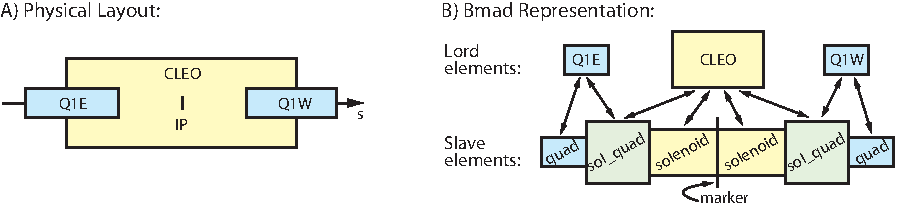
\includegraphics[width=6.0in]{superimpose-ip.pdf}
 \caption[Superposition example.]{
Superposition Example. A) Interaction region layout
with quadrupoles overlapping a solenoid. B) The Bmad lattice
representation has a list of split elements to track through and the
undivided ``lord'' elements. Pointers (double headed arrows), keep
track of the correspondence between the lords and their slaves.
 }
 \label{f:super.ip}
 \end{center}
 \end{figure}

%---------------------------------------------------------------------------

A real machine is more than a collection of independent lattice
elements. For example, the field strength in a string of elements may
be tied together via a common power supply, or the fields of different
elements may overlap.

\bmad tries to capture these interdependencies using what are referred
to as \vn{lord} and \vn{slave} elements. The \vn{lord} elements may be
divided into two classes. In one class are the \vn{controller}
elements.  These are \vn{overlay} (\sref{s:overlay}), \vn{group}
(\sref{s:group}), and \vn{girder} (\sref{s:girder}) elements that
control the attributes of other elements which are their slaves.

The other class of \vn{lord} elements embody the separation of the
physical element from the track that a particle takes when it passes
through the element. There are two types

An example will make this clear.
\vn{Superposition} (\sref{s:super}) is the ability to overlap lattice
elements spatially. \fig{f:super.ip} shows an example which is a
greatly simplified version of the IR region of Cornell's CESR storage
ring when CESR was an e+/e-- collider. As shown in \fig{f:super.ip}A,
two quadrupoles named \vn{q1w} and \vn{q1e} are partially inside and
partially outside the interaction region solenoid named \vn{cleo}. In
the lattice file, the IR region layout is defined to be
 {\small
\begin{example}
  cesr: line = (... q1e, dft1, ip, dft1, q1w ...)
  cleo: solenoid, l = 3.51, superimpose, ref = ip
\end{example}
 }
The line named \vn{cesr} ignores the solenoid and just contains the
interaction point marker element named \vn{ip} which is surrounded by
two drifts named \vn{dft1} which are, in turn, surrounded by the
\vn{q1w} and \vn{q1e} quadrupoles. The solenoid is added to the layout
on the second line by using superposition. The ``ref = ip'' indicates
that the solenoid is placed relative to \vn{ip}. The default, which is
used here, is to place the center of the superimposed \vn{cleo}
element at the center of the \vn{ip} reference element.  The
representation of the lattice in \bmad will contain two branch
\vn{sections} (``sections'' is explained more fully later): One
section, called the \vn{tracking section}, contains the elements that
are needed for tracking particles. In the current example, as shown in
\fig{f:super.ip}B, the first IR element in the tracking section is a
quadrupole that represents the part of \vn{q1e} outside of the
solenoid. The next element is a combination solenoid/quadrupole,
called a \vn{sol_quad}, that represents the part of \vn{q1e} inside
\vn{cleo}, etc.  The other branch section that Bmad creates is called
the \vn{lord section} This section contain the undivided ``physical''
\vn{super_lord} elements (\sref{s:super}) which, in this case are
\vn{q1e}, \vn{q1w}, and \vn{cleo}. Pointers are created between the
lords and their \vn{super_slave} elements in the tracking section so
that changes in parameters of the lord elements can be transferred to
their corresponding slaves.

\vn{super_lord}s are used when there are overlapping fields between
elements, the other case where there is a separation between the
physical element and the particle track comes when a particle passes
through the same physical element multiple times such as in an Energy
Recovery Linac or where different beams pass through the same element
such as in an interaction region. In this case, \vn{multipass_lords}
representing the physical element and \vn{multipass_slaves}
representing the track can be constructed (\sref{s:multipass}).
Superposition and multipass can be combined in situations where there
are overlapping fields in elements where the particle passes through

\index{no_major_lord}\index{multipass_slave}\index{slice_slave}\index{super_slave}
\index{not_a_lord}\index{group_lord}\index{girder_lord}\index{overlay_lord}
\index{multipass_lord}\index{super_lord}\index{slave_status}\index{lord_status}
Each lattice element is assigned a \vn{slave_status} indicating what kind of slave it is
and a \vn{lord_status} indicating what kind of lord it is. Normally a user does not
have to worry about this since these status attributes are handled automatically by \bmad.
The possible \vn{lord_status} settings are:
  \begin{description}
  \item[girder_lord]\Newline 
A \vn{girder_lord} element is a \vn{girder} element  (\sref{s:girder}). 
  \item[multipass_lord]\Newline
\vn{multipass_lord} elements are created when
multipass lines are present (\sref{s:multipass}). 
  \item[overlay_lord]\Newline 
An \vn{overlay_lord} is an \vn{overlay} element (\sref{s:overlay}). 
  \item[group_lord]\Newline 
A \vn{group_lord} is a \vn{group} element (\sref{s:group}).
  \item[super_lord]\Newline 
A \vn{super_lord} element is created when elements are
superimposed on top of other elements (\sref{s:super}).
  \item[not_a_lord]\Newline
This element does not control anything.
  \end{description}
Any element whose \vn{lord_status} is something other than
\vn{not_a_lord} is called a \vn{lord} element. In the \vn{tracking part}
of the branch, \vn{lord_status} will always be
\vn{not_a_lord}. In the \vn{lord section} of the branch, under normal
circumstances, there will never be any \vn{not_a_lord} elements.

Lord elements are divided into two classes. 
A \vn{major} lord represents a physical element which the slave elements are a part of.
\vn{super_lord}s and \vn{multipass_lord}s are \vn{major} lords. 
As a consequence, a \vn{major} lord is a lord that
controls nearly all of the attributes of its slaves. 
The other lords --- \vn{girder_lord}s, \vn{group_lord}s and 
\vn{overlay_lord}s --- are called \vn{minor} lords.
These lords only control some subset of a slaves attributes.

The possible \vn{slave_status} settings are
  \begin{description}
  \item[multipass_slave]\Newline
A \vn{multipass_slave} element is the slave of a \vn{multipass_lord}
(\sref{s:multipass}).
  \item[slice_slave]\Newline
A \vn{slice_slave} element represents a longitudinal slice of another element.
Slice elements are not part of the lattice but rather are created on-the-fly
when, for example, a program needs to track part way through an element.
  \item[super_slave]\Newline 
A \vn{super_slave} element is an element in the tracking part of the branch that 
has one or more \vn{super_lord} lords (\sref{s:super}).
  \item[minor_slave]\Newline
\vn{minor_slave} elements are elements that are not \vn{slice_slave}s and are only controlled
by \vn{minor} lords (\vn{overlay_lord}s, \vn{group_lord}s, or \vn{girder_lord}s).
  \item[free]\Newline
A \vn{free} element is an element with no lords.
  \end{description}

For historical reasons, each \vn{branch} in a lattice has a
\vn{tracking section} and a \vn{lord section} and the \vn{tracking
section} is always the first (lower) part of the element array and the
\vn{lord section} inhabits the second (upper) part of the array.  All
the \vn{lord} elements are put in the \vn{lord section} of branch 0
and all the other \vn{lord sections} of all the other branches are
empty.

As a side note, \'Etienne Forest's PTC code (\sref{s:ptc.intro}) uses separate
structures to separate the physical element, which PTC calls an
\vn{element} from the particle track which PTC call a \vn{fibre}.
[Actually, PTC has two structures for the physical element,
\vn{element} and \vn{elementp}. The latter being the ``polymorph''
version.] This \vn{element} and \vn{fibre} combination corresponds to
\bmad \vn{multipass_lord} and \vn{multipass_slave} elements. PTC does
not handle overlapping fields as \bmad does with \vn{superposition}
(\sref{s:super}).

%---------------------------------------------------------------------------
\section{PTC: Polymorphic Tracking Code}
\label{s:ptc.intro}
\index{PTC}

\'Etienne Forest\cite{b:forest} has written what is actually two
software libraries: FPP and PTC.  FPP stands for ``Fully Polymorphic
Package.'' What this library does is implement Taylor maps (aka
Truncated Power Series Algebra or TPSA) and Lie algebraic
operations. Thus in FPP you can define a Hamiltonian and then generate
the Taylor map for this Hamiltonian. FPP is very general. It can work
with an arbitrary number of dimensions.  FPP, however, is a purely
mathematical package in the sense that it knows nothing about
accelerator physics. That is, it does not know about bends,
quadrupoles or any other kind of element, it has no conception of a
lattice (a string of elements), it doesn't know anything about Twiss
parameters, etc. This is where PTC (Polymorphic Tracking Code) comes
in. PTC implements the high energy physics stuff and uses FPP as
the engine to do the Lie algebraic calculations.  For the purposes of
this manual, PTC and FPP are generally considered one package and the
combined PTC/FPP will be referred to as simply ``PTC''.
For programmers, interface documentation can be found in
chapter~\sref{c:ptc}.

\index{PTC!single element mode}
\bmad interfaces to PTC in two ways: One way, called ``single
element'' mode, uses PTC on a per element basis. In this case, the
method used for tracking a given element can be selected on an
element-by-element basis so non-PTC tracking methods can be mixed with
PTC tracking methods to optimize speed and accuracy. [PTC tends to be
accurate but slow.] The advantage of single element mode is the
flexibility it affords. The disadvantage is that it precludes using
PTC's analysis tools which rely on the entire lattice being tracked
via PTC. Such tools include normal form analysis beam envelope
tracking, etc.

\index{PTC!whole lattice mode}
The alternative to single element mode is ``whole lattice'' mode where
a series of PTC \vn{layout}s (equivalent to a \bmad branch) are
created from a \bmad lattice. Whether single element or whole lattice
mode (or both) is used is determined by the program being run.

%---------------------------------------------------------------------------
\section{Tao: Tool for Accelerator Optics Program}
\label{s:tao.intro}
\index{Tao}

The strength of \bmad is that, as a subroutine library, it provides a
flexible framework from which sophisticated simulation programs may
easily be developed.  The weakness of \bmad comes from its strength:
\bmad cannot be used straight out of the box. Someone must put the
pieces together into a program. To partially remedy this problem, the
\tao program\cite{b:tao} has been developed at Cornell. \tao, which uses
\bmad as its simulation engine, is a general purpose program for
simulating high energy particle beams in accelerators and storage rings.
Thus \bmad combined with \tao represents the best of both worlds: The
flexibility of a software library with the ease of use of a program.


\chapter{Lattice File Overview}
\label{c:lat.file}
\index{lattice files|hyperbf}

\index{Bmad!lattice file format}
A lattice (\sref{c:lat.concepts}) defines the sequence of elements
that a particle will travel through along with the attributes (length,
strength, orientation, etc.) of the elements.  A lattice file (or
files) is a file that is used to describe an accelerator or storage
ring. 

%---------------------------------------------------------------------------
\section{Bmad Lattice File Format}
\label{s:lattice.file.formats}

The syntax that a \bmad standard lattice file must conform to is
modeled after the lattice input format of the \mad program.
Essentially, a \bmad lattice file is similar to a \mad lattice file
except that a \bmad file has no ``action'' commands (action commands
tell the program to calculate the Twiss parameters, do tracking,
etc.).  Since \bmad is a software library, interacting with the user
to determine what actions a program should take is left to the program
and is not part of \bmad (although the \bmad library provides the
routines to perform many of the standard calculations). A program is
not required to use the \bmad parser routines but, if it does, the
following chapters describe how to construct a valid lattice file.

%---------------------------------------------------------------------------
\section{MAD, SAD, and XSIF Lattice Files}
\label{s:mad.xsif}
\index{MAD} 
\index{XSIF}

Besides being able to parse \bmad lattice files, \bmad has software to
parse XSIF\cite{b:xsif} lattice files. See \sref{s:xsif.convert} for
more details.

While \bmad cannot directly read in \mad\cite{b:maduser} or
\vn{SAD}\cite{b:sad} files, translation between \mad and \bmad lattice
files is possible using the \vn{Universal Accelerator Parser} as
discussed in Chapter~\sref{c:lat.convert}.

\newpage

%-----------------------------------------------------------------
\section{Units and Constants}
\label{s:constants}
\index{constants|hyperbf}

\bmad defines commonly used physical and mathematical constants
shown in Table~\ref{t:constants}.  All symbols use straight SI units
except for \vn{emass} and \vn{pmass} which are provided for
compatibility with \mad and should be avoided.

\begin{table}[h]
\centering
\begin{tabular}{llll} \toprule
  {\em Symbol}          & {\em Value}              & {\em Units} &  {\em Name}           \\ \midrule
  pi                    & 3.14159265359            &             &                       \\
  twopi                 & 2 * pi                   &             &                       \\
  fourpi                & 4 * pi                   &             &                       \\
  e_log                 & 2.718281828              &             &                       \\
  sqrt_2                & 1.4142135623731          &             &                       \\
  degrad                & 180 / pi                 &             & From rad to deg       \\
  degrees               & pi / 180                 &             & From deg to rad       \\
  raddeg                & pi / 180                 &             & From deg to rad       \\
  anom_moment_deuteron  & $-0.14298727047$         &             & Deuteron anomalous magnetic moment \\
  anom_moment_electron  & $0.001159652193$         &             & Electron anomalous magnetic moment \\
  anom_moment_muon      & $0.0011659208$           &             & muon anomalous magnetic moment     \\
  anom_moment_proton    & $1.79285$                &             & proton anomalous magnetic moment   \\
  fine_struct_const     & $0.00729735257$          &             & Fine structure constant            \\
  m_deuteron            & $1.875612928 \pow{9}$    & eV          & Deuteron mass         \\  
  m_electron            & $0.5109989461 \pow{6}$   & eV          & Electron mass         \\
  m_muon                & $105.6583715 \pow{6}$    & eV          & Muon mass             \\
  m_pion_0              & $134.9766 \pow{6}$       & eV          & $\pi^0$ mass          \\
  m_pion_charged        & $139.57018 \pow{6}$      & eV          & $\pi^+$, $\pi^-$ mass \\
  m_proton              & $0.9382720813 \pow{9}$   & eV          & Proton mass           \\
  c_light               & $2.99792458 \pow{8}$     & m/sec       & Speed of light        \\
  r_e                   & $2.8179403227 \pow{-15}$ & m           & Electron radius       \\
  r_p                   & $1.5346980 \pow{-18}$    & m           & Proton radius         \\
  e_charge              & $1.6021766208 \pow{-19}$ & Coul        & Electron charge       \\
  h_planck              & $4.13566733 \pow{-15}$   & eV*sec      & Planck's constant     \\
  h_bar_planck          & $6.58211899 \pow{-16}$   & eV*sec      & Planck / $2\pi$       \\
  emass                 & $0.5109989461 \pow{-3}$  & GeV         & Electron mass         \\
  pmass                 & $0.9382720813$           & GeV         & Proton mass           \\ \bottomrule
\end{tabular}
\caption{Physical and mathematical constants recognized by \bmad.}
\label{t:constants}
\end{table}

\index{mass_of}\index{anomalous_moment_of}
As an alternative, the \vn{mass_of}, and \vn{anomalous_moment_of} functions
(\sref{s:functions}) may be used in place of the defined constants for mass and anomalous
magnetic moment.

\newpage

\index{MAD!units}
\index{units!with MAD}
\bmad uses SI (Syst\`eme International) units as shown in
Table~\ref{t:units}.  Note that \mad uses different units. For example,
\mad's unit of Particle Energy is GeV not eV.

\begin{table}[ht]
\centering
\begin{tabular}{ll} \toprule
  {\em Quantity}     & {\em Units}       \\ \midrule
  Angles             &    radians        \\ 
  Betatron Phase     &    radians        \\
  Current            &    Amps           \\ 
  Frequency          &    Hz             \\ 
  Kick               &    radians        \\ 
  Length             &    meters         \\ 
  Magnetic Field     &    Tesla          \\ 
  Particle Energy    &    eV             \\ 
  RF Phase Angles    &    radians/2$\pi$ \\ 
  Voltage            &    Volts          \\ \bottomrule
\end{tabular}
\caption{Physical units used by \bmad.}
\label{t:units}
\end{table}

%---------------------------------------------------------------------------
\section{File Example and Syntax}
\index{Bmad!statement syntax}

\index{parameter statement}
\index{use statement}
The following (rather silly) example shows some of the features of a
\bmad lattice file:
\begin{example}
  ! This is a comment
  parameter[E_TOT] = 5e9                   ! Parameter definition
  pa1 = sin(3.47 * pi / c_light)                 ! Constant definition
  bend1: sbend, type = "arc bend", l = 2.3,      ! An element definition
      g = 2*pa1, tracking_method = bmad_standard
  bend2: bend1, l = 3.4                          ! Another element def
  bend2[g] = 105 - exp(2.3) / 37.5               ! Redefining an attribute
  ln1: line = (ele1, ele2, ele3)                 ! A line definition
  ln2: line = (ln1, ele4, ele5)                  ! Lines can contain lines
  arg_ln(a, b): line = (ele1, a, ele2, b)        ! A line with arguments.
  use, ln2                                       ! Which line to use for the lattice
\end{example}

\index{"! comment symbol}
\index{comment symbol ("!)}
A \bmad lattice file consists of a sequence of statements. An
exclamation mark (!) denotes a comment and the exclamation mark and
everything after the exclamation mark on a line are ignored.  \bmad is
generally case insensitive. Most names are converted to
uppercase. Exceptions where a name is not converted include file names
and atomic formulas for materials used in crystal diffraction.

\index{\& continuation symbol}
\index{continuation symbol (\&)}
Normally a statement occupies a single line in the file. Several
statements may be placed on the same line by inserting a semicolon
(``;'') between them. A long statement can occupy multiple lines by
putting an ampersand (``\&'') at the end of each line of the statement
except for the last line. Additionally, lines that end with an
``implicit continuation character''
are automatically continued to the next line. The implicit continuation 
characters are
\begin{example}
  ,   (   \{   [   =
\end{example}
Notice
that this is {\em not} like \vn{C/C++}. Thus the following is bad syntax
\begin{example}
  wall = \{
    section = \{s = 0.45     ! BAD SYNTAX. NO CONTINUATION CHARACTER HERE.
    \}                       ! BAD SYNTAX. NO CONTINUATION CHARACTER HERE.
  \}
\end{example}
Correct is:
\begin{example}
  wall = \{
    section = \{s = 0.45\} \}
\end{example}
or even:
\begin{example}
  wall = \{
    section = \{s = 0.45\} \&
  \}
\end{example}

\index{lattice files!name syntax}
Names of constants, elements, lines, etc. are limited to 40
characters. The first character must be a letter (\vn{A} --- \vn{Z}).
The other characters may be a letter, a digit (\vn{0} --- \vn{9}) or
an underscore (\vn{_}). Other characters may appear but should be avoided
since they are used by Bmad for various purposes. For example, the 
backslash (\vn{\B}) character is used to by Bmad when forming the names of
superposition slaves (\sref{s:super}) and dots (\vn{.}) are used by Bmad 
when creating names of \vn{tagged} elements (\sref{s:tag}). Also use of
special characters may make the lattice files less portable to non-Bmad programs.

\index{parameter statement}
\index{parameter statement}
\index{parameter statement}
\index{beginning statement}
The following example constructs a linear lattice with two elements: 
\begin{example}
  parameter[geometry] = open
  parameter[e_tot] =2.7389062E9
  parameter[particle] = POSITRON
  beginning[beta_a] = 14.5011548
  beginning[alpha_a] = -0.53828197
  beginning[beta_b] = 31.3178048
  beginning[alpha_b] = 0.25761815
  q: quadrupole, l = 0.6, b1_gradient = 9.011
  d: drift, l = 2.5
  t: line = (q, d)
  use, t 
\end{example}
here \vn{parameter[geometry]} (\sref{s:param}) is set to \vn{open}
which specifies that the lattice is not circular. In this case, the beginning 
Twiss parameters need to be specified and this is done by the \vn{beginning}
statements (\sref{s:beginning}). A quadrupole named \vn{q}
and a drift element named \vn{d} are specified
and the entire lattice consists of element \vn{q} followed by element \vn{d}.

%----------------------------------------------------------------------------
\section{Digested Files}
\label{s:digested}
\index{digested files}

Normally the \bmad parser routine will create what is called a
``digested file'' after it has parsed a lattice file so that when a
program is run and the same lattice file is to be read in again, to save
time, the digested file can be used to load in the lattice information.
This digested file is in binary format and is not human readable. The
digested file will contain the transfer maps for all the elements. 
Using a digested file can save considerable time if some of the
elements in the lattice need to have Taylor maps computed.
(this occurs typically with map--type wigglers).

\bmad creates the digested file in the same area as the lattice file.
If \bmad is not able to create a digested file (typically because it
does not have write permission in the directory), an error message will
be generated but otherwise program operation will be normal.

\index{ran}
\index{ran_gauss}
Digested files contain the names of the lattice files used to create
them. If a lattice file has been modified since the digested file has
been created then the lattice files will be reread and a new
digested file will be generated. 

Note: If any of the random number functions (\sref{s:functions}) are
used in the process of creating the lattice, the digested file will be
ignored. In this case, each time the lattice is read into a program,
different random numbers will be generated for expressions that use such
random numbers.

Digested files can also be used for easy transport of lattices between
programs or between sessions of a program. For example, using one
program you might read in a lattice, make some adjustments (say to model
shifts in magnet positions) and then write out a digested version of the
lattice. This adjusted lattice can now be read in by another program.

%---------------------------------------------------------------------------
\section{Element Sequence Definition}

\index{line}\index{use statement|hyperbf}
A \vn{line} defines a sequence of elements. \vn{lines} may contain
other \vn{lines} and so a hierarchy may be established. One line is
selected, via a \vn{use} statement, that defines the lattice. For
example:
\begin{example}
  l3: line = (l1, l2)   ! Concatenate two lines
  l1: line = (a, b, c)  ! Line with 3 elements
  l2: line = (a, z)     ! Another line 
  use, l3               ! Use l3 as the lattice definition.
\end{example}
In this case the lattice would be
\begin{example}
  (a, b, c, a, z)
\end{example}
\vn{Lines} can be defined in any order. See \cref{c:sequence} for more
details.

\index{superimpose}
The \vn{superimpose} construct allows elements to be placed in a
lattice at a definite longitudinal position. What happens is that
after a lattice is expanded, there is a reshuffling of the elements to
accommodate any new superimpose elements. See \sref{s:super} for more
details.

%---------------------------------------------------------------------------
\section{Lattice Elements}

The syntax for defining a lattice element roughly follows the
\mad\cite{b:maduser} program:
\begin{example}
  ele_name: keyword [, attributes]
\end{example}
where \vn{ele_name} is the element name, \vn{keyword} is the type of
element, and \vn{attributes} is a list of the elements
attributes. \cref{c:elements} gives a list of elements types with
their attributes.
\vn{Overlay} and \vn{group} type elements have a slightly different syntax:
\begin{example}
  ele_name: keyword = \{ list \}, master-attribute [= value] [, attributes]
\end{example}
and \vn{Girder} elements have the syntax
\begin{example}
  ele_name: keyword = \{ list \} [, attributes]
\end{example}  
For example:
\begin{example}
  q01w: quadrupole, type = "A String", l = 0.6, tilt = pi/2
  h10e: overlay = \{ b08e, b10e \}, var = \{hkick\}
\end{example}

%---------------------------------------------------------------------------
\section{Lattice Element Names}
\label{s:ele.names}
\index{element!names}

\index{element!name}\index{superimpose}\index{multipass}
A valid element name may be up to 40 characters in length. The first
character of the name must be a letter [A-Z]. After that, the rest of
the name can contain only letters, digits [0-9], underscore ``_'',
period ``.'', backslash ``\B'', or a hash mark ``\#''. It is best to
avoid these last three symbols since \bmad uses them to denote
``relationships''.  Periods are used for tagging (\sref{s:tag}), and
backslash and hash marks are used for to compose names for
superposition (\sref{s:super}) and multipass (\sref{s:multipass})
slave elements.

\index{reserved names}
\index{beam}\index{beam_start}\index{beginning}
\index{end}\index{parameter}\index{root}
There is a short list of names that cannot be used as an element name. 
These reserved names are:
\begin{example}
  beam
  beam_start
  beginning
  debug_marker
  end
  no_digested
  parameter
  parser_debug
  print
  root
  title
  use
\end{example}

Where appropriate, for example when setting element attributes
(\sref{s:lat.attribs}), the wild cards \vn{``*''} and \vn{``%''} can be
used to select multiple elements.  The \vn{``*''} character will match
any number of characters (including zero) while \vn{``%''} maches to
any single character. Additionally, matching can be restricted to a
certain element class using the syntax:
\begin{example}
  class::element_name
\end{example}
where \vn{class} is a class name. For example:
\begin{example}
  m*              ! Match to all elements whose name begins with "m".
  a%c             ! Match to "abc" but not to "ac" or "azzc".
  quadrupole::*w  ! Match to all quadrupoles whose name ends in "w"
\end{example}

After lattice expansion (\sref{s:expand}), the general syntax to
specify a set of elements is:
\begin{example}
  \{class::\}\{branch_id>>\}element_id\{##N\}
\end{example}
where \vn{\{...\}} marks an optional component, \vn{class} is a class
name, \vn{branch_id} is a branch name or index (\sref{s:branch.def}),
\vn{element_id} is and element name or element index
(\sref{s:lines.wo.arg}), and \vn{\#\#N} indicates that the N\Th matching
element is to be used. Examples:
\begin{example}
  quad::x_br>>q*        ! All quadrupoles of branch "x_br" whose name begins with "q".
  2>>45                 ! element \#45 of branch \#2.
  q01##3                ! The 3rd element in each branch named q01.
\end{example}

Multiple elements in a lattice may share the same name.  When
multiple branches are present, to differentiate elements that
appear in different branches, the ``branch qualified'' element name may be
used. The branch qualified element name is of the form
\begin{example}
  branch_name>>element_name
\end{example}
where \vn{branch_name} is the name of the branch and \vn{element_name}
is the ``regular'' name of the element. Example:
\begin{example}
  root>>q10w
  x_branch>>crystal3
\end{example}

For \vn{branch} lines (\sref{s:branch.def}), the full ``branch
qualified'' name of an element is of the form
\begin{example}
  branch_name>>element_name
\end{example}
where \vn{branch_name} is the name of the branch and \vn{element_name} is the
``regular'' name of the element. Example:
\begin{example}
  root>>q10w
  xline>>cryst3
\end{example}
Using the full name is only needed to distinguish elements that have
the same regular name in separate branches.  When parsing a lattice
file, branches are not formed until the lattice is expanded
(\sref{s:expand}). Therefore an \vn{expand_lattice} statement is
required before full names can be used in statements.

%---------------------------------------------------------------------------
\section{Lattice Element Attributes}
\label{s:lat.attribs}
\index{element attributes|hyperbf}

Any lattice element has various attributes like its name, its length,
its strength, etc. The values of element attributes can be
specified when the element is defined. For example:
\begin{example}
  b01w: sbend, l = 6.0, rho = 89.0 ! Define an element with attributes.
\end{example}
After an element's definition, an individual attribute may be referred
to using the syntax
\begin{example}
  class::element_name[attribute_name]
\end{example}
Element attributes can be set or used in an algebraic expression:
\begin{example}
  bo1w[roll] = 6.5                  ! Set an attribute value.
  b01w[l] = 6.5                     ! Change an attribute value.
  b01w[l] = b01w[rho] / 12          ! OK to reset an attribute value.
  my_const = b01w[rho] / b01w[l]    ! Use of attribute values in an expression.
\end{example}
Notice that there can be no space between the element name and the
\vn{[} opening bracket.  

Chapter \cref{c:elements} lists the attributes appropriate for each
element class.

When setting an attribute value, if more than one element has the
\vn{element_name} then {\it all} such elements will be set. When
setting an attribute value, if \vn{element_name} is the name of a type
of element, all elements of that type will be set. For example
\begin{example}
  q_arc[k1] = 0.234                      ! Set all elements named Q_ARC. 
  rfcavity::*[voltage] = 3.7             ! Set all RFcavity elements.
\end{example}

The wild cards \vn{``*''}, and \vn{``\%''} can be used to can be used
(\sref{s:ele.names}). Examples:
\begin{example}
  *[tracking_method] = bmad_standard  ! Matches all elements.
  quadrupole::Q*[k1] = 0.234    ! Matches all quadrupoles with names beginning with Q.
  Q%1[k1] = 0.234               ! Matches to "Q01" but not "Q001".
\end{example}
\index{beginning element}
Unlike when there are no wild cards used in a name, it is not an error
if a name with wild cards does not match to any element.
Note: A name with wild cards will never match to the \vn{BEGINNING} element (\sref{s:use}).

After lattice expansion (\sref{s:expand}), the attributes of specific elements
may be set using the syntax as discussed in Section \sref{s:ele.names}. Example:
\begin{example}
  expand_lattice              ! Expand the lattice.
  97[x_offset] = 0.0023       ! Set x_offset attribute of 97th element
  b2>>si_cryst##2[tilt] = 0.1 ! Tilt the 2nd instance of "si_cryst" in branch "b2" 
\end{example}

%---------------------------------------------------------------------------
\section{Custom Element Attributes}
\label{s:cust.att}
\index{element attributes!defining custom attributes}

Real scalar and vector custom element attributes may be defined for any class of
element.  Custom element attributes are useful with programs that need
to associate ``extra'' information with particular lattice elements
and it is desired that this extra information be settable from within
a lattice file. For example, a program might need error tolerance
for the strength of quadrupoles.

Adding custom attributes will not disrupt programs that are not designed to use the custom
attributes. Currently, up to five scalar (that is, single valued) custom attributes may be
defined for any given element type. The syntax for defining custom attributes is:
\begin{example}
  parameter[custom_attributeN] = "\{class::\}attribute_name"
\end{example}
Where ``\vn{N}'' is an integer between 1 and 5 and
"\vn{attribute_name}" is the name of the attribute. To restrict the
custom attribute to a particular element class, the element class can
be prefixed to the attribute name. Examples:
\begin{example}
  parameter[custom_attribute1] = "mag_id"
  parameter[custom_attribute1] = "quadrupole::error_k1"
  parameter[custom_attribute2] = "color"
\end{example}
The first line in the example assigns a custom attribute name of
\vn{mag_id} to all elements.  The second line in the example overrides
the setting of \vn{custom_attribute1} for quadrupole elements only. 

Once a custom attribute has been defined it may be set for an element
of the correct type. Example:
\begin{example}
  parameter[custom_attribute2] = "lcavity::rms_phase_err"
  ...
  l2a: lcavity, rms_phase_err = 0.0034, ...
\end{example}

For someone creating a program, section~\sref{s:ele.gen} describes how
to make the appropriate associations.

Note: If custom string information needs to be associated with an
element, the \vn{type}, \vn{alias} and \vn{descrip} element components
(\sref{s:alias}) are available.

\index{r_custom}
There is a three dimensional vector custom attribute called \vn{r_custom} that can be set.
For example:
\begin{example}
  qq: quadrupole, r_custom(-2,1,5) = 34.5, r_custom(-3) = 77.9
\end{example}
Negative indices are accepted and if only one or two indices are present, the others
are assumed to be zero. Thus \vn{r_custom(-3)} is equivalent to \vn{r_custom(-3,0,0)}.

%---------------------------------------------------------------------------
\section{Variable Types}
\label{s:var.types}
\index{arithmetic expressions!variables}

\index{logicals|hyperbf}
There are five types of variables in \bmad: reals, integers, switches,
logicals (booleans), and strings. Acceptable logical values are
\begin{example}
   true    false
   t       f
\end{example}
For example
\begin{example}
  rf1[is_on] = False
\end{example}

\index{strings|hyperbf}
String literals can be quoted using double quotes (") or single quotes ('). 
If there are no
blanks or commas within a string, the quotes can be omitted. For example:
\begin{example}
  Q00W: Quad, type = "My Type", alias = Who_knows, &
                                  descrip = "Only the shadow knows"
\end{example}
Unlike most everything else, strings are not converted to uppercase.

\index{switches|hyperbf}
Switches are variables that take discrete values. For example:
\begin{example}
  parameter[particle] = positron          
  q01w: quad, tracking_method = bmad_standard 
\end{example}
The name ``switch'' can refer to the variable (for example,
\vn{tracking_method}) or to a value that it can take (for example,
\vn{bmad_standard}). The name ``method'' is used interchangeably with switch.

%---------------------------------------------------------------------------
\section{Arithmetic Expressions}
\index{arithmetic expressions} 
\label{s:arith}

Arithmetic expressions can be used in a place where a real value is required.
The standard operators are defined: \hfil\break
\hspace*{0.15in}
\begin{tabular}{ll}
  $a + b$           & Addition        \\
  $a - b$           & Subtraction     \\
  $a \, \ast \, b$  & Multiplication  \\
  $a \; / \; b$     & Division        \\
  $a \, ^{\scriptstyle\wedge} \, b$ & Exponentiation  \\
\end{tabular}
\hfil\break
\bmad also has a set of intrinsic functions. A list of these is given
in \sref{s:functions}.

\index{arithmetic expressions!constants}
Literal constants can be entered with or without a decimal point. An
exponent is marked with the letter E. For example
\begin{example}
  1, 10.35, 5E3, 314.159E-2
\end{example}
Symbolic constants can be defined using the syntax
\begin{example}
  constant_name = expression
\end{example}
\index{MAD!syntax compatibility with BMAD}
Alternatively, to be compatible with \mad, using ``:='' instead of ``='' is accepted
\begin{example}
  constant_name := expression
\end{example}
Examples:
\begin{example}
  my_const = sqrt(10.3) * pi^3
  abc     := my_const * 23
\end{example}
\index{MAD!delayed substitution}
Unlike \mad, \bmad uses immediate substitution so that all constants
in an expression must have been previously defined. For example, the
following is {\em not} valid:
\begin{example}
  abc      = my_const * 23      ! No: my_const needs to be defined first.
  my_const = sqrt(10.3) * pi^3
\end{example}
here the value of \vn{my_const} is not known when the line ``\vn{abc}
= $\ldots$'' is parsed. Once
defined, symbolic constants cannot be redefined. For example:
\begin{example}
  my_const = 1
  my_const = 2  ! No: my_const cannot be redefined.
\end{example}

\index{group}\index{overlay}\index{lattice expansion}
\vn{group} (\sref{s:group}) and \vn{overlay} (\sref{s:overlay}) controller elements are an
exception to the immediate evaluation rule. Since controller elements may control elements
that do not exist until \vn{lattice expansion} (\sref{s:expand}), the arithmetic
expressions associated with controller elements are not evaluated until lattice expansion.
Example:
\begin{example}
  s_20W: sextupole, l = 0.27
  sk: overlay = \{s_20W[a1]:-2*s_20W[l]\}, var = \{k1\}, k1 = 0.2
  s_20W[l] = 0.34
  s_30E: s_20W
  ...
  expand_lattice
\end{example}
Here the expression of overlay \vn{sk} is evaluated, when the lattice is expanded, to be
\vn{-0.68 = -2*0.34}. This uses uses the length of element \vn{s_20W} at the point when
the lattice is expanded and not at the point when \vn{sk} was defined. Additionally, the
element \vn{s_30E}, which inherits the attributes of \vn{s_20W}, inherits a value of zero
for \vn{a1} (skew multipole moment) since inheritance uses immediate evaluation just like
the setting of constants.


Element attributes can be used after they have been defined but not
before.  Example:
\begin{example}
  sa: sextupole, l = 0.3, k2 = 0.01 * sa[l]  ! Good
  sb: sextupole, k2 = 0.01 * sb[l], l = 0.3  ! BAD SET OF K2. L IS DEFINED AFTER.
\end{example}
In this example, the \vn{k2} attribute of element \vn{sa} is correctly
set since \vn{k2} is defined after \vn{l}. On the other hand, \vn{k2}
of element \vn{sb} will have a value of zero since \vn{l} of \vn{sb}
defaults to zero before it is set.

One potential pitfall with immediate substitution is that when
an element attribute changes, it does not affect prior evaluations.
Example:
\begin{example}
  s1: sextupole, k2 = 2.3
  aa = s1[k2]              ! aa = 2.3
  s1[k2] = 1.7             ! value of aa does not change
\end{example}
Here the value of constant \vn{aa} will remain fixed at 2.3 no matter how
the value of \vn{s1[k2]} is altered after \vn{aa} is defined.

Another potential pitfall is when using
dependent element attributes (\sref{s:depend}). For example:
\begin{example}
  b01w: sbend, l = 0.5, angle = 0.02
  a_const = b01w[g]    ! No: bend g has not yet been computed!
\end{example}
Here the bend strength \vn{g} (\sref{s:bend}) will eventually be
computed to be 0.04 (= angle / l) but that computation does not happen
until lattice expansion (\sref{s:expand}). In this case, the value of
\vn{a_const} will be the default value of \vn{g} which is zero.  As a
rule of thumb, never rely on dependent attributes having their correct
value.

%---------------------------------------------------------------------------
\section{Intrinsic functions}
\label{s:functions}
\index{intrinsic functions}

\index{sqrt}\index{log}\index{exp}\index{sin}\index{cos}\index{tan}\index{factorial}
\index{asin}\index{acos}\index{atan}\index{abs}\index{ran}\index{ran_gauss}
\index{mass_of}\index{charge_of}\index{anomalous_moment_of}\index{species}
The following intrinsic functions are recognized by \bmad: \hfil\break
\hspace*{0.15in}
\begin{tabular}{ll}
  \vn{sqrt}(x)                  & Square Root                                    \\
  \vn{log}(x)                   & Logarithm                                      \\
  \vn{exp}(x)                   & Exponential                                    \\
  \vn{sin}(x)                   & Sine                                           \\
  \vn{cos}(x)                   & Cosine                                         \\
  \vn{tan}(x)                   & Tangent                                        \\
  \vn{asin}(x)                  & Arc sine                                       \\
  \vn{acos}(x)                  & Arc cosine                                     \\
  \vn{atan}(x)                  & Arc Tangent                                    \\
  \vn{atan2}(y, x)              & Arc Tangent of y/x                             \\
  \vn{abs}(x)                   & Absolute Value                                 \\
  \vn{factorial}(n)             & Factorial                                      \\
  \vn{ran}()                    & Random number between 0 and 1                  \\
  \vn{ran_gauss}()              & Gaussian distributed random number             \\
  \vn{int}(x)                   & Nearest integer with magnitude less then x     \\
  \vn{nint}(x)                  & Nearest integer to x                           \\
  \vn{floor}(x)                 & Nearest integer less than x                    \\
  \vn{ceiling}(x)               & Nearest integer greater than x                 \\
  \vn{mass_of}(A)               & Mass of particle A                             \\
  \vn{charge_of}(A)             & Charge, in units of the elementary charge, of particle A \\
  \vn{anomalous_moment_of}(A)   & Anomalous magnetic moment of particle A        \\
  \vn{species}(A)               & Species ID of A
\end{tabular}

\index{ran_seed}
\vn{ran_gauss} is a Gaussian distributed random number with unit RMS. 
Both \vn{ran} and \vn{ran_gauss} use a seeded random number generator. 
To choose the seed set 
\begin{example}
  parameter[ran_seed] = <Integer>
\end{example}
A \vn{value} of zero will set the seed using the system clock so that
different sequences of random numbers will be generated each time a
program is run.  The default behavior if \vn{parameter[ran_seed]} is
not present is to use the system clock for the seed.

\index{expand_lattice}
If an element is used multiple times in a lattice, and if \vn{ran} or
\vn{gauss_ran} is used to set an attribute value of this element, then
to have all instances of the element have different attribute values
the setting of the attribute must be after the lattice has been
expanded (\sref{s:expand}). For example:
\begin{example}
  a: quad, ... 
  a[x_offset] = 0.001*ran_gauss()
  my_line: line = (a, a)
  use, my_line
\end{example}
Here, because \bmad does immediate evaluation, the \vn{x_offset}
values for \vn{a} gets set in line 2 and so both copies of \vn{a} in
the lattice get the same value. This is probably not what is wanted.
On the other hand if the attribute is set after lattice expansion:
\begin{example}
  a: quad, ...
  my_line: line = (a, a)
  use, my_line
  expand_lattice
  a[x_offset] = 0.001*ran_gauss()
\end{example}
Here the two \vn{a} elements in the lattice get different values for
\vn{x_offset}.

The \vn{mass_of}, \vn{charge_of}, and \vn{anomalous_moment_of} functions give the mass of,
charge of (in units of the elementary charge), and anomalous moment of, a particle.
Example:
\begin{example}
  parameter[particle] = deuteron
  am = anomalous_moment_of(parameter[particle])^2
  my_particle = species(He++)      ! my_particle now represents He++
  chg1 = charge_of(my_particle)    ! chg = charge of He++
  chg2 = charge_of(He++)           ! Same as previous line
  chg3 = charge_of(species(He++))  ! Same as previous line
\end{example}
The \vn{species} function is needed in the definition of \vn{my_particle} so that \bmad knows that
the string ``He++'' represents a type of particle. Inside functions like \vn{mass_of}, the use of
\vn{species} is optional since, in this case, \bmad can correctly parse the argument.

%-----------------------------------------------------------------------------
\section{Statement Order}
\label{s:state.order}
\index{statement order|hyperbf}

With some exceptions, statements in a lattice file can be in any order. For example, the lines
(\sref{s:lines.wo.arg}) specified in a \vn{use} statement (\sref{s:use}) can come after the \vn{use}
statement. And \vn{group} (\sref{s:group}) and \vn{overlay} (\sref{s:overlay}) controller elements
may be defined before the slave elements whose parameters they control are defined.

The exceptions to this rule are:
\begin{itemize}
\item 
If there is an \vn{expand_lattice} statement (\sref{s:expand.lat}), everything necessary for
lattice expansion must come before. In particular, all \vn{line}s
(\sref{s:lines.wo.arg}), \vn{list}s (\sref{s:replace.list}), and \vn{use} (\sref{s:use}) statements
necessary for lattice expansion must come before.
\item
Immediate evaluation of arithmetic expressions (\sref{s:arith}) mandates that values be defined
before use.
\item
A lattice element must be defined before any of its parameters are set. Example:
\begin{example}
  pp[z_offset] = 0.1    ! WRONG! PP HAS NOT BEEN DEFINED YET!
  pp: patch             ! Here PP is defined
\end{example}
In this example, the \vn{z_offset} of the element \vn{pp} is set before \vn{pp} has been
defined. This is an error. As a corollary to this rule, element parameters that are set 
using wild card characters will only affect those parameters that have been already defined. For
example:
\begin{example}
  crystal::*[b_param] = 0.2
  c5: crystal
\end{example}
In this example, the \vn{b_param} of all \vn{crystal} elements is set to \vn{0.2} {\em except} for
\vn{c5} and all other crystal elements that are defined after the set.
\end{itemize}

%-----------------------------------------------------------------------------
\section{Print Statement}
\label{s:print}
\index{print statement|hyperbf}

The \vn{print} statement prints a message at the terminal when the 
lattice file is parsed by a program. Syntax:
\begin{example}
  print <String>
\end{example}
For example
\begin{example}
  print Remember! Q01 quad strength not yet optimized!
\end{example}
The \vn{print} statement is useful to remind someone using the lattice of important details.

%-----------------------------------------------------------------------------
\section{Title Statement}
\index{title statement|hyperbf}

The \vn{title} statement sets a title string which can be used by a program. 
For consistency with \mad there are two possible syntaxes
\begin{example}
  title, <String>
\end{example}
or the statement can be split into two lines
\begin{example}
  title
  <String>
\end{example}
For example
\begin{example}
  title
  "This is a title"
\end{example}

%--------------------------------------------------------------------------
\section{Call Statement}
\label{s:call}
\index{call statement|hyperbf}

It is frequently convenient to separate the lattice definition into
several files.  Typically there might be a file (or files) that define
the layout of the lattice (something that doesn't change often) and a
file (or files) that define magnet strengths (something that changes
more often).  The \vn{call} is used to read in separated lattice
files. The syntax is
\begin{example}
  call, filename = <String>
\end{example}
Example:
\begin{example}
  call, filename = "../layout/my_layout.bmad"      ! Relative pathname
  call, filename = "/nfs/cesr/lat/my_layout.bmad"  ! Absolute pathname
\end{example}
\bmad will read the called file until a \vn{return} or \vn{end_file}
statement is encountered or the end of the file is reached.

For filenames that have a relative pathname, the called file will be
searched for relative to the directory of the calling file.  Thus, in
the above example, if the file containing the call statements is in the
directory \vn{/path/to/lat_dir}, the first call will open the file:
\begin{example}
  /path/to/lat_dir/../layout/my_layout.bmad 
\end{example}

Where a called file is searched for may be modified by using a
\vn{use_local_lat_file} statement. See Section~\sref{s:use.loc} for
more details.

An XSIF (\sref{s:lattice.file.formats}) lattice file may be called
from within a \bmad lattice file by prepending \vn{"xsif::"} to the
file name. Example:
\begin{example}
  call, filename = "xsif::my_lattice.xsif"
\end{example}
This statement must be the first statement in the \bmad lattice file
except for any comments or debugging statements (\sref{s:debug}). 
The XSIF lattice file must define a
complete lattice and cannot contain any \bmad specific statements. The
call to the XSIF file automatically expands the lattice
(\sref{s:expand}) and any additional statements in the \bmad lattice
file operate on the expanded lattice.

%--------------------------------------------------------------------------
\section{Inline Call}
\label{s:call.inline}
\index{call!inline}

Any lattice elements will have a set of attributes that need to be defined.
As a convenience, it is possible to segregate an element attribute or attributes
into a separate file and then ``call'' this file using an
``inline call''. The inline call has three forms. In an element definition,
the inline call has the form
\begin{example}
  <ele_name>: <ele_type>, ..., call::<file_name>, ...
\end{example}
or
\begin{example}
  <ele_name>: <ele_type>, ..., <attribute_name> = call::<file_name>, ...
\end{example}
where \vn{<attribute_name>} is the name of the attribute and
\vn{<file_name>} is the name of the where the attribute structure is
given.  The third form of the inline call occurs when an element
attribute is redefined and has the form
\begin{example}
  <ele_name>[<attribute_name>] = call::<file_name>
\end{example}
Example:
\begin{example}
  c: crystal, call::my_curvature.bmad, surface = call::my_surface.bmad, ...
\end{example}  

Inline calls can be used to call binary files (useful for speeding up lattice parcing).
See \sref{s:binary.form} for more details.

%--------------------------------------------------------------------------
\section{Binary Format}
\label{s:binary.form}
\index{binary format lattice files}

It is possible to store certain element attributes in a binary format file which is useful for
speeding up lattice parcing. These binary files must have a \vn{.bin} suffix. The attributes
that support binary files are:
\begin{example}
  cartesian_map       ! \sref{s:cart.map}
  cylindrical_map     ! \sref{s:cylind.map}
  grid_field          ! \sref{s:grid.field}
  taylor_field        ! \sref{s:taylor.field}
\end{example}

The syntax for calling a binary file is the same as an inline call (\sref{s:call.inline}).
Example:
\begin{example}
  qq: quadrupole, grid_field = call::my_grid.bin, ...
\end{example}

To create a binary file or files, first create a lattice with the attributes defined with plain
text. Next read the lattice into any program that can create \bmad lattice files (for example, the
\tao program (\sref{s:tao.intro}) can do this) and have the program generate a lattice file.

%--------------------------------------------------------------------------
\section{Use_local_lat_file Statement}
\label{s:use.loc}
\index{use_local_lat_file_statement|hyperbf}

It is sometimes convenient to override where \bmad looks for called
files (see \sref{s:call}). For example, suppose it is desired to
temporarily override the settings in a called file without modifying
the called file itself. In this case, the \vn{use_local_lat_file}
statement can be used. When this statement is encountered in a lattice
file, the local directory (that is, the directory from which the
program is run) is searched first for the called file and if a file
of the correct name is found, that file is used.

An example will make this clear. Suppose lattice file \vn{/A/lat.bmad}
contains the call:
\begin{example}
  call, filename = "/B/sub.bmad"
\end{example}
Now suppose that you want to use \vn{lat.bmad} with a modified
\vn{sub.bmad} but you do not want to modify \vn{/A/lat.bmad} or
\vn{/B/sub.bmad}. The solution is to create two new files. One file,
call it \vn{new.bmad}, which can be situated in any directory, has two
lines in it:
\begin{example}
  use_local_lat_file
  call, filename = "/A/lat.bmad"
\end{example}
The second new file is the modified \vn{sub.bmad} and it must be in the
directory from which the program is run.

%--------------------------------------------------------------------------
\section{Return and End_File Statements}
\index{return statement|hyperbf}
\index{end_file statement|hyperbf}

\vn{Return} and \vn{end_file} have identical effect and tell \bmad to
ignore anything beyond the \vn{return} or \vn{end_file} statement in
the file.

%----------------------------------------------------------------------------
\section{Expand_Lattice Statement}
\label{s:expand.lat}
\index{expand_lattice|hyperbf}

Normally, lattice expansion happens automatically at the end of the parsing of the lattice file but
an explicit \vn{expand_lattice} statement in a lattice file will cause immediate expansion. See
\sref{s:expand} for details.

%----------------------------------------------------------------------------
\section{Lattice Expansion}
\label{s:expand}
\index{lattice!expansion|hyperbf}

At some point in parsing a lattice file, the ordered sequence (or sequences if there are multiple
branches) of elements that form a lattice must be constructed. This process is called \vn{lattice
expansion} since the element sequence can be built up from sub--sequences
(\sref{c:sequence}). Normally, lattice expansion happens automatically at the end of the parsing of
the lattice file (or files) but an explicit \vn{expand_lattice} statement in a lattice file will cause
immediate expansion. The reason why lattice expansion may be necessary before the end of the file is
due to the fact that some operations need to be done after lattice expansion. This includes:
\begin{Itemize}
\item 
\index{ran}
\index{ran_gauss}
The \vn{ran} and \vn{ran_gauss} functions, when used with elements
that show up multiple times in a lattice, generally need to be used
after lattice expansion. See \sref{s:functions}.
\item
Some dependent variables may be set as if they are independent
variables but only if done before lattice expansion. See \sref{s:depend}.
\index{multipass}
\item 
Setting the \vn{phi0_multipass} attribute for an 
\vn{Lcavity} or \vn{RFcavity} multipass
slave may only be done after lattice expansion (\sref{s:multipass}).
\item
\index{tags for Lines and Lists}
Setting individual element attributes for tagged elements can only be done
after lattice expansion (\sref{s:tag}).
\end{Itemize}

Notice that all \vn{line}s (\sref{s:lines.wo.arg}), \vn{list}s (\sref{s:replace.list}), and \vn{use}
(\sref{s:use}) statements necessary for lattice expansion must come before an \vn{expand_lattice}
statement.

Lattice expansion is only done once so it is an error if multiple
\vn{expand_lattice} statements are present.

The steps used for lattice expansion are:
\begin{enumerate}
\item
Instantiate all of the lines listed in the last \vn{use} statement (\sref{s:use}). If an instantiated line has
\vn{fork} or \vn{photon_fork} (\sref{s:fork}) elements, instantiate the lines connected to the fork
elements if the \vn{fork} or \vn{photon_fork} is connected to a new branch. Instantiation of a given
line involves:
\begin{enumerate}
\item
Line expansion (\sref{c:sequence}) where the element sequence is constructed from the line and sub-lines.
\item
Adding any superpositions (\sref{s:super}).
\end{enumerate}
\item
Form multipass lords and mark the appropriate multipass slaves (\sref{s:multipass}).
\item
Add girder control elements (\sref{s:girder}).
\item
Add group (\sref{s:group}) and overlay (\sref{s:overlay}) control elements.
\end{enumerate}

\index{secondary lattice file}
A lattice file where all the statements are post lattice expansion
valid is called a ``\vn{secondary lattice file}''.  To promote
flexibility, \bmad has methods for parsing lattices in a two step
process: First, a ``primary'' lattice file that defines the basic
lattice is read. After the primary lattice has been parsed and lattice
expansion has been done, the second step is to read in one or more
secondary lattice files. Such secondary lattice files can be used, for
example, to set such things as element misalignments. The point here
is that there are no calls (\sref{s:call}) of the secondary files in
the primary file so the primary lattice file does not have to get
modified when different secondary files are to be used.

%--------------------------------------------------------------------------
\section{Debugging Statements}
\label{s:debug}
\index{no_digested statement}
\index{no_superimpose statement}
\index{parser_debug statement}
\index{debug_marker statement}
\index{no_digested statement}
\index{lattice files!parser debugging}

There are a few statements
which can help in debugging the \bmad lattice parser
itself. That is, these statements are generally only used by programmers.
These statements are:
\begin{example}
  debug_marker
  no_digested
  no_superimpose
  parser_debug
\end{example}

The \vn{debug_marker} statement is used for marking a place in the lattice file
where program execution is to be halted. This only works when running
a program in conjunction with a program debugging tool. 

The \vn{no_digested} statement if present, will prevent \bmad from 
creating a digested file (\sref{s:digested}. That is, the lattice file will always
be parsed when a program is run.

The \vn{no_superimpose} statement is used to suppress superpositions
(\sref{s:super}). This is useful for debugging purposes.

The \vn{parser_debug} statement will cause information about the
lattice to be printed out at the terminal. It is recommended that this
statement be used with small test lattices since it can generate a lot
of output. The syntax is
\begin{example}
  parser_debug <switches>
\end{example}
Valid \vn{<switches>} are
\begin{example}
  beam_start          ! Print the beam_start information.
  ele <n1> <n2> ...   ! Print full info on selected elements.
  lattice             ! Print a list of lattice element information.
  lord                ! Print full information on all lord elements.
  seq                 ! Print sequence information.
  slave               ! Print full information on all slave elements.
  var                 ! Print variable information.
\end{example}
Here $<n1>$, $<n2>$, etc. are the index of the selected elements in
the lattice.  Example
\begin{example}
  parser_debug var lat ele 34 78
\end{example}


\chapter{Elements}
\label{c:elements}
\index{element|hyperbf}

A lattice is made up of a collection of elements --- quadrupoles,
bends, etc. This chapter discusses the various types of elements
available in \bmad.

\begin{table}[htb]
\centering
{\tt
\begin{tabular}{llll} \toprule
  {\it Element}     & {\it Section}       & {\it Element}      & {\it Section}    \\ \midrule
  AB_Multipole      & \ref{s:ab.m}        &  Match             & \ref{s:match}    \\ 
  AC_Kicker         & \ref{s:ac.kick}     &  Monitor           & \ref{s:monitor}  \\
  BeamBeam          & \ref{s:bbi}         &  Multipole         & \ref{s:mult}     \\
  Beginning_Ele     & \ref{s:begin.ele}   &  Null_Ele          & \ref{s:null.ele} \\
  Bend_Sol_Quad     & \ref{s:bsq}         &  Octupole          & \ref{s:oct}      \\
  Custom            & \ref{s:custom}      &  Patch             & \ref{s:patch}    \\
  Drift             & \ref{s:drift}       &  Photon_Fork       & \ref{s:fork}     \\
  E_Gun             & \ref{s:e.gun}       &  Pipe              & \ref{s:monitor}  \\
  Ecollimator       & \ref{s:col}         &  Quadrupole        & \ref{s:quad}     \\
  ElSeparator       & \ref{s:elsep}       &  Rbend             & \ref{s:bend}     \\
  EM_Field          & \ref{s:em.field}    &  Rcollimator       & \ref{s:col}      \\
  Fiducial          & \ref{s:fiducial}    &  RFcavity          & \ref{s:rfcav}    \\
  Floor_Shift       & \ref{s:floor.ele}   &  Sad_Mult          & \ref{s:sad.mult} \\
  Fork              & \ref{s:fork}        &  Sbend             & \ref{s:bend}     \\
  HKicker           & \ref{s:hvkicker}    &  Sextupole         & \ref{s:sex}      \\
  Hybrid            & \ref{s:hybrid}      &  Sol_Quad          & \ref{s:sq}       \\
  Instrument        & \ref{s:monitor}     &  Solenoid          & \ref{s:sol}      \\
  Kicker            & \ref{s:kicker}      &  Taylor            & \ref{s:taylor}   \\
  Lcavity           & \ref{s:lcav}        &  Undulator         & \ref{s:wiggler}  \\
  Marker            & \ref{s:mark}        &  VKicker           & \ref{s:hvkicker} \\  
  Mask              & \ref{s:mask}        &  Wiggler           & \ref{s:wiggler}  \\ \bottomrule
\end{tabular}
}
\caption{Table of element types suitable for use with charged particles.}
\label{t:particle.classes}\center
\end{table}

\index{MAD}
Most element types available in \mad are provided in \bmad.
Additionally, \bmad provides a number of element types that are not
available in \mad.  A word of caution: In some cases where both \mad
and \bmad provide the same element type, there will be an overlap of
the attributes available but the two sets of attributes will not be
the same.  The list of element types known to \bmad is shown in
Table~\ref{t:particle.classes}, \ref{t:photon.classes}, and
\ref{t:control.classes}.  Table~\ref{t:particle.classes} lists the
elements suitable for use with charged particles,
Table~\ref{t:photon.classes} which lists the elements suitable for use
with photons, and finally Table~\ref{t:control.classes} lists the
\vn{controller} element types that can be used for parameter control
of other elements. Note that some element types are suitable for both
particle and photon use.

\begin{table}[ht]
\centering
{\tt
\begin{tabular}{llll} \toprule
  {\it Element}      & {\it Section}         & {\it Element}       & {\it Section}      \\ \midrule
  Beginning_Ele      & \ref{s:begin.ele}     &  Marker             & \ref{s:mark}       \\
  Capillary          & \ref{s:capillary}     &  Mask               & \ref{s:mask}       \\
  Crystal            & \ref{s:crystal}       &  Match              & \ref{s:match}      \\
  Custom             & \ref{s:custom}        &  Monitor            & \ref{s:monitor}    \\ 
  Detector           & \ref{s:detector}      &  Mirror             & \ref{s:mirror}     \\
  Diffraction_Plate  & \ref{s:diff.plate}    &  Multilayer_Mirror  & \ref{s:multilayer} \\
  Drift              & \ref{s:drift}         &  Patch              & \ref{s:patch}      \\
  Ecollimator        & \ref{s:col}           &  Photon_Fork        & \ref{s:fork}       \\
  Fiducial           & \ref{s:fiducial}      &  Photon_Init        & \ref{s:photon.init}\\
  Floor_Shift        & \ref{s:floor.ele}     &  Pipe               & \ref{s:monitor}    \\
  Fork               & \ref{s:fork}          &  Rcollimator        & \ref{s:col}        \\
  Instrument         & \ref{s:monitor}       &  Sample             & \ref{s:sample}     \\ \bottomrule
\end{tabular}
}
\caption{Table of element types suitable for use with photons.}
\label{t:photon.classes}\center
\end{table}

\begin{table}[ht]
\centering
{\tt
\begin{tabular}{llll} \toprule
  {\it Element}  & {\it Section}     & {\it Element}  & {\it Section}    \\ \midrule
  Group          & \ref{s:group}     &  Overlay       & \ref{s:overlay}  \\
  Girder         & \ref{s:girder}    &                &                  \\ \bottomrule
\end{tabular}
}
\caption{Table of controller elements.}
\label{t:control.classes}\center
\end{table}

For a listing of element attributes for each type of element, see Chapter~\sref{c:attrib.list}.

%-----------------------------------------------------------------
\section{AB_Multipole}
\label{s:ab.m}
\index{ab_multipole|hyperbf}

An \vn{ab_multipole} is a thin magnetic multipole lens up to 21\St order. The
basic difference between this and a \vn{multipole} (\sref{s:mult} is
the input format. See section~\sref{s:mag.field} for how the multipole
coefficients are defined.

General \vn{ab_multipole} attributes are:
\begin{center}
\tt 
\begin{tabular}{llll} \toprule
  {\sl Attribute Class}      & \s               & {\sl Attribute Class}      & \s              \\ \midrule
  a$n$, b$n$ multipoles      & \ref{s:multip}   & Length                     & \ref{s:l}       \\
  Aperture limits            & \ref{s:limit}    & Offsets \& tilt            & \ref{s:offset}  \\
  Chamber wall               & \ref{s:wall}     & Reference energy           & \ref{s:energy}  \\ 
  Custom Attributes          & \ref{s:cust.att} & Superposition              & \ref{s:super}   \\
  Description strings        & \ref{s:alias}    & Tracking \& transfer map   & \ref{c:methods} \\
  Is_on                      & \ref{s:is.on}    &                            &                 \\
  \bottomrule
\end{tabular}
\end{center}
\toffset
See \sref{s:list.ab.multipole} for a full list of element attributes.

\index{x_pitch}\index{y_pitch}
The length \vn{l} is a fictitious length that is used for synchrotron
radiation computations and affects the longitudinal position of the
next element but does not affect any tracking or transfer map
calculations.  The \vn{x_pitch} and \vn{y_pitch} attributes are not
used in tracking.

When an \vn{ab_multipole} is superimposed (\sref{s:super}) on a lattice, it is
treated as a zero length element and in this case it is an error for the length
of the \vn{ab_multipole} to be set to a nonzero value.

Unlike a \vn{multipole}, an \vn{ab_multipole} will {\em not} affect the
reference orbit if there is a dipole component. 

Example:
\begin{example}
  abc: ab_multipole, a2 = 0.034e-2, b3 = 5.7, a11 = 5.6e6/2
\end{example}

%-----------------------------------------------------------------
\section{AC_Kicker}
\label{s:ac.kick}
\index{ab_kicker|hyperbf}

An \vn{ac_kicker} element simulates a time dependent kicker element.

General \vn{ac_kicker} attributes are:
\begin{center}
\tt
\begin{tabular}{llll} \toprule
  {\sl Attribute Class}      & Section           & {\sl Attribute Class}      & Section         \\ \midrule
  Aperture limits            & \ref{s:limit}     & Is_on                      & \ref{s:is.on}   \\
  Chamber wall               & \ref{s:wall}      & Length                     & \ref{s:l}       \\
  Custom Attributes          & \ref{s:cust.att}  & Mag \& Elec multipoles     & \ref{s:multip}  \\
  Description strings        & \ref{s:alias}     & Offsets, pitches \& tilt   & \ref{s:offset}  \\
  Field Maps                 & \ref{s:fieldmap}  & Reference energy           & \ref{s:energy}  \\ 
  Fringe Fields              & \ref{s:fringe}    & Superposition              & \ref{s:super}   \\
  Hkick \& Vkick             & \ref{s:kick}      & Symplectify                & \ref{s:symp}    \\
  Integration settings       & \ref{s:integ}     & Tracking \& transfer map   & \ref{c:methods} \\
  \bottomrule
\end{tabular}
\end{center}
\toffset
See \sref{s:list.ac.kicker} for a full list of element attributes.

Attributes specific to a \vn{bend_sol_quad} element are:
\begin{example}
  t_offset   = <Real>                                      ! Time offset of field waveform.
  amp_vs_time = \{(<t1>, <A1>), (<t2>, <A2>), ...\}          ! Field amplitude vs Time.
  frequencies = \{(<f1>, <A1>, <phi1>), (<f2>, <A2>, <phi2>), ...\} ! Frequency components.
\end{example}
Note: The units of the phases \vn{phi} with the \vn{frequencies} attribute are \vn{radians/2pi}.

An \vn{ac_kicker} element is like a \vn{kicker} element except that the field varies in time. The
field is calculated in two steps:
\begin{enumerate}
\item Calculate the field the same as for a \vn{kicker} element (\sref{s:kicker}).
\item Scale the field by the function $A(t-t_0)$ where $t$ is the time and $t_0$ is set
by the \vn{t_offset} attribute. 
\end{enumerate}
The time is calculated, like the RF cavities, using either relative or absolute time (\sref{s:rf.time}).

There are two ways to specify the dimensionless time variation $A(t)$ of the field. One way is to
specify points on the $A(t)$ curve using the \vn{amp_vs_time}
attribute. Example:
\begin{example}
  mk: ac_kicker, l = 0.3, scale_multipoles = F, b1 = 0.27, t_offset = 3.6e-8,
          amp_vs_time = \{(-1.2e-6, 0.02), ... \} 
\end{example}
The element in this example is an AC quadrupole kicker. The times (in seconds) must be in assending
order and no two times may be the same. \bmad uses a cubic spline fit
to interpolate between the time points. For times outside of the range specified by
\vn{amp_vs_time}, the amplitude is taken to be zero.

The second way to specify $A(t)$ is to specify the frequencies in the $A(t)$ spectrum using the
\vn{frequencies} attribute:
\Begineq
  A(t) = \sum_i \, A_i \, \cos( 2 \, \pi (f_i \, t + \phi_i))
\Endeq
Example:
\begin{example}
  mk: ac_kicker, l = 0.3, field_calc = fieldmap, cartesian_map = \{...\},
          frequencies = \{(3.4e6, 0.34, 0.12), ...\}
\end{example}
Note: The units of the phases \vn{phi} with the \vn{frequencies} attribute are \vn{radians/2pi}.

Note: The calculated field will only obey Maxwell's equations in the limit that the time variation
of the field is ``slow'':
\Begineq
  \omega \ll \frac{c}{r}
\Endeq
where $\omega$ is the characteristic frequency of the field variation, $c$ is the speed of light,
and $r$ is the characteristic size of the \vn{ac_kicker} element. That is, the fields at opposite ends
of the element must be able to ``communicate'' in a time scale short compared to the time scale of
the change in the field.

%-----------------------------------------------------------------
\section{BeamBeam}
\label{s:bbi}
\index{beambeam|hyperbf}

A \vn{beambeam} element simulates an interaction with an opposing
(``strong'') beam traveling in the opposite direction. The strong beam
is assumed to be Gaussian in shape. In the \vn{bmad_standard}
calculation the beam--beam kick is computed using the
Bassetti--Erskine complex error function formula\cite{b:talman}

General \vn{beambeam} attributes are:
\begin{center} 
\tt
\begin{tabular}{llll} \toprule
  {\sl Attribute Class}      & Section          & {\sl Attribute Class}      & Section         \\ \midrule
  Aperture limits            & \ref{s:limit}    & Is_on                      & \ref{s:is.on}   \\
  Chamber wall               & \ref{s:wall}     & Offsets, pitches \& tilt   & \ref{s:offset}  \\
  Custom Attributes          & \ref{s:cust.att} & Reference energy           & \ref{s:energy}  \\
  Description strings        & \ref{s:alias}    & Superposition              & \ref{s:super}   \\
  Is_on                      & \ref{s:is.on}    & Tracking \& transfer map   & \ref{c:methods} \\ 
  \bottomrule
\end{tabular}
\end{center}
\toffset
See \sref{s:list.beambeam} for a full list of element attributes.

\index{sig_x}\index{sig_y}\index{sig_z}
\index{n_slice}\index{charge}\index{bbi_constant}
\index{beta_a}\index{beta_b}\index{alpha_a}\index{alpha_b}
Attributes specific to a \vn{beambeam} element are:
\begin{example}
  sig_x   = <Real>     ! Horizontal strong beam sigma at the center 
  sig_y   = <Real>     ! Vertical strong beam sigma at the center
  sig_z   = <Real>     ! Strong beam length
  charge  = <Real>     ! Strong beam charge. Default = -1
  n_slice = <Integer>  ! Number of strong beam slices
  beta_a  = <Real>     ! $a$-mode beta Twiss parameter
  alpha_a = <Real>     ! $a$-mode alpha Twiss parameter 
  beta_b  = <Real>     ! $b$-mode beta Twiss parameter
  alpha_b = <Real>     ! $b$-mode alpha Twiss parameter 
  bbi_constant         ! See below. Dependent attribute (\sref{s:depend}).
\end{example}

\index{n_part!in BeamBeam element}
The number of particles in the strong beam is set by
\begin{example}
  charge * parameter[n_part]
\end{example}
\vn{parameter[n_part]} is the nominal number of particles of the strong
beam. \vn{parameter[n_part]} is a global setting (\sref{s:param}) and is 
used for all \vn{beambeam} elements. 
To vary the number of particles in an individual \vn{beambeam} element,
the \vn{charge} attribute is used.
The default is \vn{charge} = -1 which indicates
that the strong beam has the opposite charge of the weak beam.

\index{sig_z}\index{n_slice}
\vn{sig_z} are the strong beam's longitudinal sigma.
The strong beam is divided up into \vn{n_slice} equal charge (not
equal thickness) slices. Propagation through the strong beam involves
a kick at the charge center of each slice with drifts in between the
kicks. The kicks are calculated using the standard Bassetti--Erskine
complex error function formula\cite{b:talman}.  Even though the strong
beam can have a finite \vn{sig_z}, the length of the element is always
considered to be zero. This is achieved by adding drifts at either end
of any tracking so that the longitudinal starting point and ending
point are identical. The longitudinal $s$--position of the
\vn{BeamBeam} element is at the center of the strong bunch. For
example, with \vn{n_slice} = 2 the calculation would proceed as
follows:
\begin{enumerate}
  \item  Start with the reference particle at the center of the strong bunch.
  \item  Propagate (drift) backwards to the center of the first slice.
  \item  Apply the beam--beam kick due to the first slice.
  \item  Propagate (drift) forwards to the center of the second slice.
  \item  Apply the beam--beam kick due to the second slice.
  \item  Propagate (drift) backwards to end up with the reference particle
     at the center of the strong bunch.
\end{enumerate}

\index{sig_x}\index{sig_y}
\index{beta_a}\index{beta_b}\index{alpha_a}\index{alpha_b}
\vn{sig_x}, \vn{sig_y} are the transverse sigmas of the strong beam
at $s_0$ which is the $s$-position where the \vn{beambeam} element is located. 
For calculating the the sigmas of any given slice, \vn{sig_x} and \vn{sig_y} 
are extrapolated using the Twiss parameters at $s_0$. The Twiss parameters
at $s_0$ are set by \vn{beta_a}, \vn{beta_b}, \vn{alpha_a}, and \vn{alpha_b}.
If \vn{beta_a} is zero (the default), the $a$-mode Twiss parameters as 
calculated from the lattice is used. Similarly, 
if \vn{beta_b} is zero (the default), the $b$-mode Twiss parameters as 
calculated from the lattice is used.


\index{x_offset}\index{y_offset}\index{z_ofset}
\index{x_pitch}\index{y_pitch}
\vn{x_offset}, \vn{y_offset}, and \vn{z_offset} are used to offset the
\vn{beambeam} element. Note that in \mad the attributes used to
offset the strong beam are called \vn{xma} and \vn{yma}.
\vn{x_pitch} and \vn{y_pitch} gives the beam--beam interaction a
crossing angle. This is the full crossing angle, not the half-angle.

The \vn{bbi_constant} is a measure of the beam--beam interaction
strength.  It is a dependent variable and is calculated from the
equation
\Begineq
  C_{bbi} = N \, m_e \, r_e / (2 \, \pi \, \gamma \, (\sigma_x + \sigma_y))
\Endeq
In the linear region, near $x = y = 0$, the 
beam--beam kick is approximately 
\begin{align}
  k_x &= -4\, \pi \, x \, C_{bbi} / \sigma_x \CRNO
  k_y &= -4\, \pi \, y \, C_{bbi} / \sigma_y 
\end{align}

The beam--beam tune shift is 
\begin{align}
  dQ_x &= C_{bbi} \, \beta_x / \sigma_x \CRNO
  dQ_y &= C_{bbi} \, \beta_y / \sigma_y \CRNO
\end{align}

Example:
\begin{example}
  parameter[n_part] = 1.34e10     ! Used for all beambeam eles
  bbi: beambeam, sig_x = 3e-3, sig_y = 3e-4, x_offset = 0.05
\end{example}

%-----------------------------------------------------------------
\section{Beginning_Ele}
\label{s:begin.ele}
\index{beginning_ele|hyperbf}

An \vn{beginning_ele} element, named \vn{BEGINNING}, is placed at the beginning of every
branch (\sref{s:branch.def}) of a lattice to mark the start of the branch. The
\vn{beginning_ele} always has element index 0 (\sref{c:lat.concepts}). The creation of
this \vn{beginning_ele} element is automatic and it is not permitted for a lattice file to
define any other \vn{beginning_ele} elements.

\vn{beginning_ele} attributes are generally set using either \vn{parameter}
(\sref{s:param}) or \vn{beginning} (\sref{s:beginning}) statements.
In particular the initial energy may be set (\sref{s:energy}).

%-----------------------------------------------------------------
\section{Bend_Sol_Quad}
\label{s:bsq}
\index{bend_sol_quad|hyperbf}

A \vn{bend_sol_quad} is a combination bend, solenoid, and quadrupole
with the solenoid strength varying linearly with longitudinal position.
This enables the simulation of solenoid edge fields. 

General \vn{bend_sol_quad} attributes are:
\begin{center}
\tt
\begin{tabular}{llll} \toprule
  {\sl Attribute Class}      & Section           & {\sl Attribute Class}      & Section          \\ \midrule
  Mag \& Elec multipoles     & \ref{s:multip}    &                            &                  \\
  Aperture limits            & \ref{s:limit}     & Length                     & \ref{s:l}        \\
  Chamber wall               & \ref{s:wall}      & Offsets, pitches \& tilt   & \ref{s:offset}   \\
  Custom Attributes          & \ref{s:cust.att}  & Overlapping Fields         & \ref{s:overlap}  \\
  Description strings        & \ref{s:alias}     & Reference energy           & \ref{s:energy}   \\
  Fringe fields              & \ref{s:fringe}    & Symplectify                & \ref{s:symp}     \\
  Hkick \& Vkick             & \ref{s:kick}      & Field Maps                 & \ref{s:fieldmap} \\
  Is_on                      & \ref{s:is.on}     & Tracking \& transfer map   & \ref{c:methods}  \\
  \bottomrule
\end{tabular}
\end{center}
\toffset

\index{x_quad}\index{y_quad}\index{quad_tilt}\index{tilt}
\index{dks_ds}\index{g}\index{bend_tilt}\index{angle}
\index{rho}\index{k1}\index{ks}
Attributes specific to a \vn{bend_sol_quad} element are:
\begin{example}
  g           = <Real>    ! Bend strength 1/rho
  b_field     = <Real>    ! Design field strength (= P_0 g / q) (\sref{s:depend}).
  angle       = <Real>    ! Bend angle. A settable dependent variable (\sref{s:depend})
  rho         = <Real>    ! Bend radius. A settable dependent variable (\sref{s:depend})
  bend_tilt   = <Real>    ! Bend tilt angle. See \sref{s:offset}.
  k1          = <Real>    ! Quad strength.
  b1_gradient = <Real>    ! Quadrupole Field strength.
  x_quad      = <Real>    ! Quad horizontal offset.
  y_quad      = <Real>    ! Quad vertical offset.
  quad_tilt   = <Real>    ! Quad tilt. See \sref{s:offset}.
  ks          = <Real>    ! Solenoid strength.
  bs_field    = <Real>    ! Solenoid Field strength.
  dks_ds      = <Real>    ! Solenoid field variation.      
  tilt        = <Real>    ! Overall tilt. See \sref{s:offset}
\end{example}
See \sref{s:list.bend.sol.quad} for a full list of element attributes.

The magnetic
field is:
\begin{alignat}{1}
  \frac{q \, B_x}{P_0} &= -g_y + k_{1n} (y - y_q) - k_{1s} (x - x_q) - \frac{dks/ds}{2} \, x \CRNO
  \frac{q \, B_y}{P_0} &=  g_x + k_{1n} (x - x_q) + k_{1s} (y - y_q) - \frac{dks/ds}{2} \, y \CR
  \frac{q \, B_s}{P_0} &=  k_s + dks/ds                        \nonumber
\end{alignat}
The reference trajectory is along the solenoid centerline. The
quadrupole field is offset from the solenoid by (\vn{x_quad},
\vn{y_quad}). The quadrupole and bend have individual tilts
\vn{quad_tilt} and \vn{bend_tilt} respectively.  \vn{tilt} gives an
overall tilt. Thus the normal and skew quadrupole components $k_{1n}$,
and $k_{1s}$ are given by
\begin{example}
  k_1n = k1 * cos (2*(tilt + quad_tilt))
  k_1s = k1 * sin (2*(tilt + quad_tilt))
\end{example}
and the dipole bend components ($g_x$, $g_y$) are given by
\begin{example}
  g_x = g * cos (tilt + bend_tilt)
  g_y = g * sin (tilt + bend_tilt)
\end{example}
Dipole edge fields have not been implemented since it is not clear
where the entrance and exit faces (\sref{s:ref.construct}) of the bend
should be and how they are aligned with the solenoid.

To simulate a real solenoid you will need at least three
\vn{bend_sol_quad} elements: The middle element is the body of the
solenoid with the linear solenoid strength \vn{dks_ds} = 0 and the two
end elements have nonzero \vn{dks_ds} to simulate the solenoid edges.

Currently, tracking through a \vn{Bend_Sol_Quad} is via symplectic integration only.
\vn{bmad_standard} tracking is not an option since there is a possibility in
the future to implement tracking via a closed formula. 
Example:
\begin{example}
  bsq: bend_sol_quad, l = 3.7, ks = -2.3, dks_ds = 4.7, g = 1/87
\end{example}

%-----------------------------------------------------------------
\section{Bends: Rbend and Sbend}
\label{s:bend}
\index{sbend|hyperbf}
\index{rbend|hyperbf}

\vn{Rbend}s and \vn{sbend}s are dipole bends. 

General \vn{rbend} and \vn{sbend} attributes are:
\begin{center}
\tt
\begin{tabular}{llll} \toprule
  {\sl Attribute Class}      & Section           & {\sl Attribute Class}      & Section          \\ \midrule
  Aperture limits            & \ref{s:limit}     & Mag \& Elec multipoles     & \ref{s:multip}   \\ 
  Chamber wall               & \ref{s:wall}      & Offsets, pitches \& tilt   & \ref{s:offset}   \\
  Custom Attributes          & \ref{s:cust.att}  & Overlapping Fields         & \ref{s:overlap}  \\
  Description strings        & \ref{s:alias}     & Reference energy           & \ref{s:energy}   \\ 
  Fringe Fields              & \ref{s:fringe}    & Superposition              & \ref{s:super}    \\
  Hkick \& Vkick             & \ref{s:kick}      & Symplectify                & \ref{s:symp}     \\
  Is_on                      & \ref{s:is.on}     & Field Maps                 & \ref{s:fieldmap} \\
  Integration settings       & \ref{s:integ}     & Tracking \& transfer map   & \ref{c:methods}  \\
  Length                     & \ref{s:l}         &                            &                  \\
  \bottomrule
\end{tabular}
\end{center}
\toffset
See \sref{s:list.bend} for a full list of element attributes.

\index{g}\index{b_field}\index{g_err}\index{b_field_err}\index{angle}
\index{l_chord}\index{angle}\index{h1}\index{h2}
\index{e1}\index{e2}\index{fint}\index{fintx}\index{l_arc}
\index{hgap}\index{hgapx}\index{roll}\index{k1}\index{exact_multipoles}
Attributes specific to \vn{rbend} and \vn{sbend} elements are:
\begin{example}
  angle              = <Real>     ! Design bend angle. A settable dependent var (\sref{s:depend}).
  b_field            = <Real>     ! Design field strength (= P_0 g / q) (\sref{s:depend}).
  b_field_err        = <Real>     ! Field strength error (\sref{s:depend}).
  b1_gradient        = <Real>     ! Quadrupole field strength (\sref{s:depend}).
  b2_gradient        = <Real>     ! Sextupole field strength (\sref{s:depend}).
  e1, e2             = <Real>     ! Face angles.
  exact_multipoles   = <Switch>   ! Curved coordinate correction? \vn{off} is default.
  fint, fintx        = <Real>     ! Face field integrals.
  g                  = <Real>     ! Design bend strength (= 1/rho).
  g_err              = <Real>     ! Bend strength error (\sref{s:depend}).
  h1, h2             = <Real>     ! Face curvature.
  hgap, hgapx        = <Real>     ! Pole half gap.
  k1                 = <Real>     ! Quadrupole strength.
  k2                 = <Real>     ! Sextupole strength (\sref{s:depend}).
  l                  = <Real>     ! ``Length'' of bend. See below.
  l_arc              = <Real>     ! Arc length. For \vn{rbend}s only. 
  l_chord                         ! Chord length. Dependent attribute. See \sref{s:l}.
  n_ref_pass         = 0 or 1     ! Multipass reference turn (\sref{s:multipass}).
  ptc_field_geometry = <Switch>   ! See below.
  rho                = <Real>     ! Design bend radius. A settable dependent var (\sref{s:depend}).
  roll               = <Real>     ! See \ref{s:offset}.
\end{example}

\begin{figure}[tb]
  \centering
  \hfill
  \begin{subfigure}[b]{0.45\textwidth}
    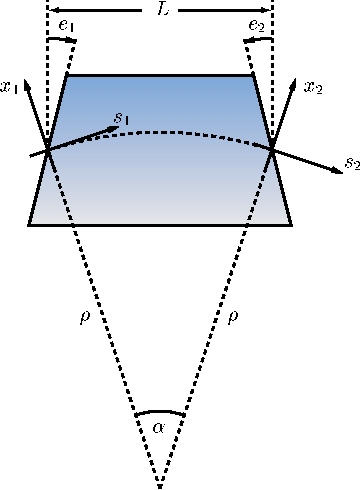
\includegraphics{rbend-coords.pdf}
    \caption{rbend}
    \label{f:bend.rbend}
  \end{subfigure}
  \hfill
  \begin{subfigure}[b]{0.45\textwidth}
    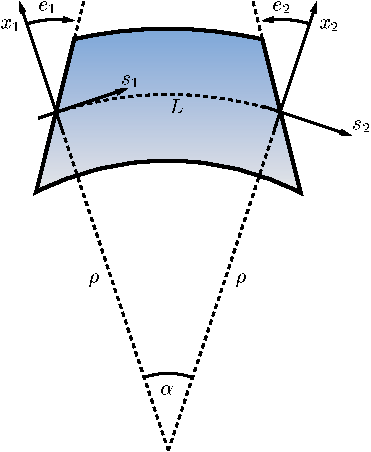
\includegraphics{sbend-coords.pdf}
    \caption{sbend}
    \label{f:bend.sbend}
  \end{subfigure}
  \hfill
  \caption[Coordinate systems for (a) \vn{rbend}\ and (b) \vn{sbend}\ elements.]
{Coordinate systems for (a) \vn{rbend} and (b) \vn{sbend} elements.
For the bends drawn as viewed from ``above'' (viewed from positive $y$),
\vn{g}, \vn{angle}, \vn{rho}, \vn{e1} and \vn{e2} are all positive.}
  \label{f:bend}
\end{figure}

  \begin{description}
  \index{angle}
  \item[angle] \Newline
The total design bend angle. A positive \vn{angle} represents a
bend towards negative $x$ values (see \fig{f:local.coords}).
  \index{e1}\index{e2}
  \item[e1, e2] \Newline
The rotation angle of the entrance pole face is \vn{e1} and at the exit face it is
\vn{e2}. Zero \vn{e1} and \vn{e2} for an \vn{rbend} gives a rectangular magnet
(\fig{f:bend.rbend}). Zero \vn{e1} and \vn{e2} for an \vn{sbend} gives a wedge shaped magnet
(\fig{f:bend.sbend}).  An \vn{sbend} with an \vn{e1} = \vn{e2} = \vn{angle}/2 is equivalent to
an \vn{rbend} with \vn{e1} = \vn{e2} = 0 (see above).  This formula holds for both
positive and negative angles.

Note: The correspondence between \vn{e1} and \vn{e2} and the
corresponding SAD parameters is:
\begin{example}
  e1(Bmad) =  e1(SAD) * angle + ae1(SAD)
  e2(Bmad) =  e2(SAD) * angle + ae2(SAD)
\end{example}
  \index{exact_multipoles}
  \item[exact_multipoles] \Newline
The \vn{exact_multipoles} switch can be set to one of:
\begin{example}
  off                 ! Default
  vertically_pure    
  horizontally_pure  
\end{example}
This switch determines if the multipole fields, both magnetic and electric, and including
the \vn{k1} and \vn{k2} components, are corrected for the finite curvature of the
reference orbit in a bend. See \sref{s:field.exact} for a discussion of what
\vn{vertically} pure versus \vn{horizontally} pure means. Setting \vn{exact_multipoles} to
\vn{vertically_pure} means that the individual $a_n$ and $b_n$ multipole components are
used with the vertically pure solutions
\begin{align}
  \bfB &= \sum_{n = 0}^\infty \left[ \frac{a_n}{n+1} \nabla \phi_n^r + \frac{b_n}{n+1} \nabla \phi_n^i \right] \nonumber
  \bfE &= \sum_{n = 0}^\infty \left[ \frac{a_{en}}{n+1} \nabla \phi_n^i + \frac{b_{en}}{n+1} \nabla \phi_n^r \right]
\end{align}
and if \vn{exact_multipoles} is set to \vn{horizontally_pure} the horizontally pure solutions
$\psi_n^r$ and $\psi_n^i$ are used instead of the vertically pure solutions $\phi_n^r$ and
$\phi_n^i$.

To use exact multipoles with PTC based tracking (\sref{c:methods}), the PTC exact model
tracking must be turned on. That is, in the lattice file set:
\begin{example}
  parameter[ptc_exact_model] = T
\end{example}
With exact model tracking, PTC always assumes that multipole coefficients correspont to
\vn{horizontally_pure}. In this case, \bmad will convert \vn{vertically_pure} to
\vn{horizontally_pure} as needed when passing multipole coefficients to PTC. Note that in
the case where PTC is doing exact model tracking (\sref{s:integ}) but the
\vn{exact_multipoles} switch is set to \vn{off}, PTC will still be treating the multipoles
as \vn{horizontally_pure} even though \bmad tracking will be treating them as straight
line multipoles. Note: If the bend has an associated electric field, PTC will always be
doing exact modeling.

  \index{fint}\index{fintx}\index{hgapx}\index{hgapx}
  \item[fint, fintx, \Newline hgap, hgapx] \Newline
The field integrals for the entrance and
exit pole faces are give by \vn{fint} and \vn{fintx} respectively
\Begineq
  F_{int} = \int_{pole} \! \! ds \, \frac{B_y(s) \, (B_{y0} - B_y(s))}
  {2 \, H_{gap} \, B_{y0}^2}
  \label{fsbbb}
\Endeq
with a similar equation for \vn{fintx}. In the equation $B_{y0}$ is the field in the
interior of the dipole and $H_{gap}$ is the pole half gap.  The parameters \vn{hgap} and
\vn{hgapx} are the half gaps at the entrance and exit faces. If \vn{fint} or \vn{fintx} is
given without a value then a value of 0.5 is used. If \vn{fint} or \vn{fintx} is not
present, the default value of 0 is used. Note: \mad does not have the \vn{fintx} and
\vn{hgapx} attributes. \mad just assumes that the values are the same for the entrance and
exit faces. For compatibility with \mad, if \vn{fint} is given but \vn{fintx} is not, then
\vn{fintx} is set equal to \vn{fint}. Similarly, \vn{hgapx} will be set to \vn{hgap} if
\vn{hgapx} is not given.

Note: The SAD program uses \vn{fb1+f1} for the entrance fringe and
\vn{fb2+f1} for the exit fringe. The correspondence between the two is
\begin{example}
  fint  * hgap  = (fb1 + f1) / 12
  fintx * hgapx = (fb2 + f1) / 12
\end{example}

\index{Enge function}
\vn{fint} and \vn{hgap} can be related to the Enge function which is sometimes
used to model the fringe field. The Enge function is of the form
\Begineq
  B_y(s) = \frac{B_{y0}}{1 + \exp[P(s)]}
\Endeq
where
\Begineq
  P(s) = C_0 + C_1 \, s + C_2 \, s^2 + C_3 \, s^3 + \, \ldots
\Endeq
The $C_0$ term simply shifts where the edge of the bend is. If all the $C_n$
are zero except for $C_0$ and $C_1$ then 
\Begineq
  C_1 = \frac{1}{2 \,H_{gap} \, F_{int}}
\Endeq
  \index{g}\index{rho}\index{g_err}
  \item[g, g_err, rho] \Newline
The design bending radius which determines the reference coordinate
system is \vn{rho} (see \sref{s:ref}). \vn{g} = 1/\vn{rho} is
the curvature function and is proportional to the design dipole
magnetic field. The true field strength is given by
\vn{g}~+~\vn{g_err} so changing \vn{g_err} leaves the design orbit
unchanged but varies a particle's orbit.
  \index{h1}\index{h2}
  \item[h1, h2] \Newline
The attributes \vn{h1} and \vn{h2} are the curvature of the entrance
and exit pole faces. They are present for compatibility with MAD but
are not yet implemented in terms of tracking and other calculations.
  \index{k1}\index{b1_gradient}
  \item[k1, b1_gradient] \Newline
The normalized and unnormalized quadrupole strength.
  \index{k2}\index{b2_gradient}
  \item[k2, b2_gradient] \Newline
The normalized and unnormalized sextupole strength. 
  \index{l}\index{l_chord}\index{l_arc}
  \item[l, l_arc, l_chord]  \Newline
For compatibility with MAD, for an \vn{rbend}, \vn{l} is the chord
length and not the arc length as it is for an \vn{sbend}.  However,
after reading in a lattice, \bmad will internally convert all
\vn{rbend}s into \vn{sbend}s, additionally, the \vn{l_chord} attribute
will be set to the input \vn{l}, and \vn{l} will be set to the true
path length (see above). Alternatively for an \vn{rbend}, instead of
setting \vn{l}, the \vn{l_arc} attribute can be set to the true arc
length.
  \index{ref_tilt}
  \item[ref_tilt] \Newline
The \vn{ref_tilt} attribute rotates a bend about the longitudinal axis
at the entrance face of the bend. \vn{ref_tilt} = 0 bends the bends
the element in the $-y$ direction. See \fig{f:tilt.bend}. It is
important to understand that \vn{ref_tilt}, unlike the \vn{tilt}
attribute of other elements, bends both the reference orbit along with
the physical element. Note that the MAD \vn{tilt} attribute for bends
is equivalent to the \bmad \vn{ref_tilt}. Bends in \bmad do not have
a \vn{tilt} attribute.
  \end{description}

%---------------

\index{l}
The difference between \vn{rbend} and \vn{sbend} elements
is the way the \vn{l}, \vn{e1}, and \vn{e2} attributes are interpreted.
To ease the bookkeeping burden, after reading in a lattice, \bmad will
internally convert all \vn{rbend}s into \vn{sbend}s. 
This is done using the following transformation on \vn{rbend}s:
\begin{example}
  l_chord(internal) = l(input)
  l(internal) = 2 * asin(l_chord * g / 2) / g
  e1(internal) = e1(input) + theta / 2
  e2(internal) = e2(input) + theta / 2
\end{example}

The attributes \vn{g}, \vn{angle}, and \vn{l} are mutually dependent. If any two are
specified for an element \bmad will calculate the appropriate value
for the third.  After reading in a lattice, \vn{angle} is considered a
dependent variable (\sref{s:depend}).

Since internally all \vn{rbend}s are converted to \vn{sbend}s, if one wants to
vary the \vn{g} attribute of a bend and still keep the bend rectangular, an
overlay (\sref{s:overlay}) can be constructed to maintain the proper face angles.
For example:
\begin{example}
  l_ch = 0.54
  g_in = 1.52
  l_coef = asin(l_ch * g_in / 2) / g_in
  my_bend: rbend, l = l_ch, g = g_in
  my_overlay: overlay = \{my_bend, my_bend[e1]:l_coef, my_bend[e2]:l_coef\}, 
                var = \{g\}, g = g_in
\end{example}
Notice that \vn{l_coef} is just \vn{arc_length/2}.

The \vn{n_ref_pass} attribute are only used when a bend is part of a \vn{multipass} line and is used
to set the reference geometry of the bend. See section~\sref{s:multipass} for more details.

In the local coordinate system (\sref{s:ref}), looking from ``above'' (bend viewed from positive
$y$), and with \vn{ref_tilt} = 0, a positive \vn{angle} represents a particle rotating clockwise. In
this case. \vn{g} will also be positive. For counterclockwise rotation, both \vn{angle} and \vn{g}
will be negative but the length \vn{l} is always positive. Also, looking from above, a positive
\vn{e1} represents a clockwise rotation of the entrance face and a positive \vn{e2} represents a
counterclockwise rotation of the exit face. This is true irregardless of the sign of \vn{angle} and
\vn{g}. Also it is always the case that the pole faces will be parallel when
\begin{example}
  e1 + e2 = angle
\end{example}

\begin{figure}[tb]
  \centering
  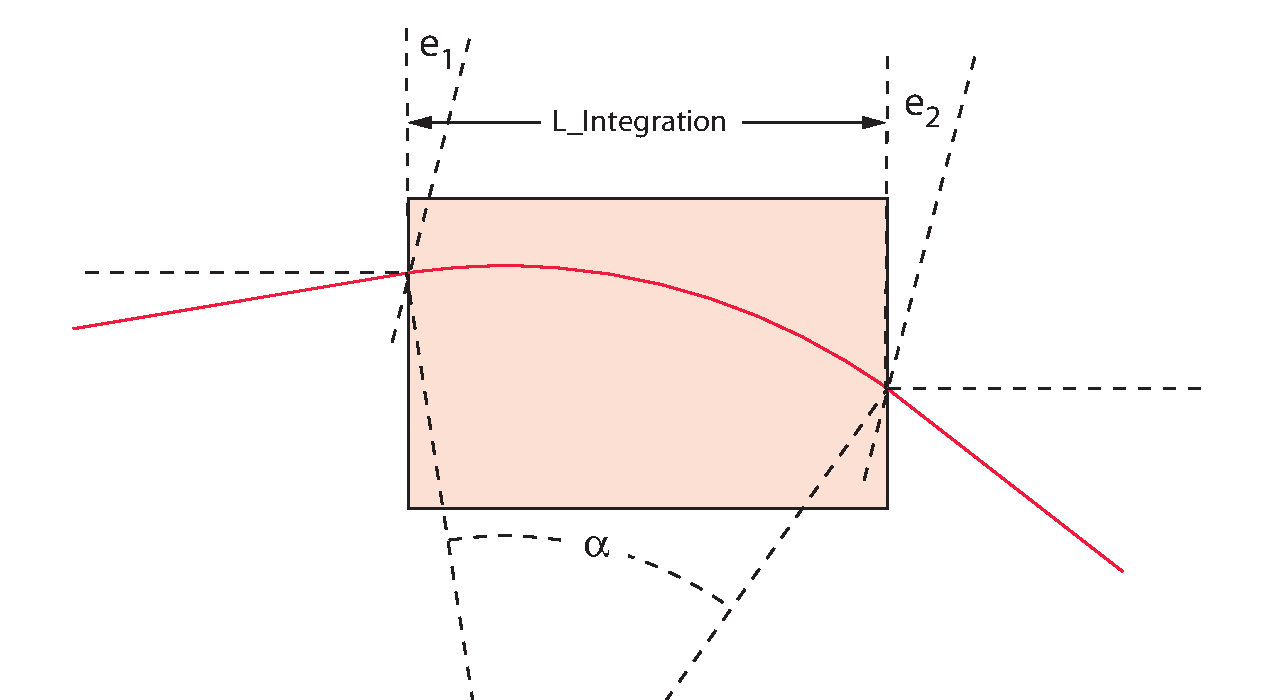
\includegraphics[width=5in]{true-rbend.pdf}
  \caption[True Rbend coordinates]{Coordinate system when \vn{ptc_field_geometry}
is set to \vn{true_rbend}.}
  \label{f:true.rbend}
\end{figure}

Example bend specification:
\begin{example}
  b03w: sbend, l = 0.6, k1 = 0.003, fint  ! gives fint = fintx = 0.5
\end{example}


\vn{ptc_field_geometry} determines how PTC integrates through a bend
if PTC is being used for tracking. Possible values for
\vn{ptc_field_geometry} are:
\begin{example}
  sector      ! Default
  straight
  true_rbend  ! Only valid for rbend elements
\end{example}
For \vn{sector} tracking, the tracking coordinate reference frame is
with respect to the arc of the reference trajectory. For \vn{straight}
tracking the tracking coordinate reference frame is with respect to the
chord line. For a bend where the number of integration steps is large
enough, and where there are no other fields besides the basic dipole
field, the results are the same.  When there are quadrupole or higher
order fields, the fields are expanded about the tracking reference
frame. Since Maxwell's equations must be satisfied, the higher order
fields will differ when tracking with \vn{sector} vs \vn{straight} the
difference in the fields will scale with the inverse of the bending
radius \vn{1/rho}. The above discussion is true for
\vn{ptc_exact_model} set to True, for \vn{ptc_exact_model} set to
False, a simplified sector tracking model is used in all cases.

The \vn{true_rbend} tracking of \vn{ptc_field_geometry} is used only
with \vn{rbend} elements and the entrance and exit faces must be parallel
as shown in \fig{f:true.rbend}. That is
\begin{example}
  e1 + e2 = 0
\end{example}
In this case, the tracking geometry is parallel, to the bend face as
shown in the figure. This can be an advantage in some situations but
\'Etienne Forest discourages use of \vn{true_rbend} due to complications
of how to handle the reference frames. In particular, how to handle
the reference frames is problematic when you have more than one of
them in a row.

%-----------------------------------------------------------------
\section{Capillary}
\label{s:capillary}
\index{capillary|hyperbf}

A \vn{capillary} element is a glass tube that is used to focus x-ray
beams.

General \vn{capillary} attributes are:
\begin{center}
\tt
\begin{tabular}{llll} \toprule
  {\sl Attribute Class}      & Section          & {\sl Attribute Class}      & Section         \\ \midrule
  Aperture limits            & \ref{s:limit}    & Offsets, Pitches \& Tilt   & \ref{s:offset}  \\ 
  Capillary Wall             & \ref{s:wall}     & Reference energy           & \ref{s:energy}  \\
  Custom Attributes          & \ref{s:cust.att} & Tracking \& transfer map   & \ref{c:methods} \\ 
  Description strings        & \ref{s:alias}    &                            &                 \\
  \bottomrule
\end{tabular}
\end{center}
\toffset
See \sref{s:list.capillary} for a full list of element attributes.

\index{critical_angle_factor|hyperbf}
Attributes specific to a \vn{capillary} element are:
\begin{example}
  critical_angle_factor = <Real>    ! Critical angle * Energy (rad * eV)
\end{example}

The critical angle above which photons striking the capillary surface are
refracted into the capillary material scales as 1/Energy. The
constant of critical angle * energy is given by the \vn{critical_angle_factor}.

The inside wall of a capillary is defined using the same syntax used
to define the chamber wall for other elements (\sref{s:wall}).

The length of the capillary is a dependent variable and is given by
the value of \vn{s} of the last wall cross-section
(\sref{s:wall.capillary}).

%-----------------------------------------------------------------
\section{Collimators: Ecollimator and Rcollimator} 
\label{s:col}
\index{ecollimator|hyperbf}
\index{rcollimator|hyperbf}

An \vn{ecollimator} is a drift with elliptic collimation. An \vn{rcollimator} is a drift
with rectangular collimation.

Alternatively, for defining a collimator with an arbitrary shape, a \vn{mask} element
(\sref{s:mask}) may be used.

General \vn{ecollimator} and \vn{rcollimator} attributes are:
\begin{center}
\tt
\begin{tabular}{llll} \toprule
  {\sl Attribute Class}      & Section          & {\sl Attribute Class}      & Section          \\ \midrule
  Aperture limits            & \ref{s:limit}    & Offsets, Pitches \& Tilt   & \ref{s:offset}   \\
  Chamber wall               & \ref{s:wall}     & Overlapping Fields         & \ref{s:overlap}  \\
  Custom Attributes          & \ref{s:cust.att} & Reference energy           & \ref{s:energy}   \\
  Description strings        & \ref{s:alias}    & Superposition              & \ref{s:super}    \\
  Hkick \& Vkick             & \ref{s:kick}     & Symplectify                & \ref{s:symp}     \\
  Integration settings       & \ref{s:integ}    & Field Maps                 & \ref{s:fieldmap} \\
  Length                     & \ref{s:l}        & Tracking \& transfer map   & \ref{c:methods}  \\
  \bottomrule
\end{tabular}
\end{center}
\toffset

Note: Collimators are the exception to the rule that the aperture is
independent of any \vn{tilt}s. See \sref{s:limit} for more
details. Additionally, the default setting of
\vn{offset_moves_aperture} is \vn{True} for collimators (\sref{s:offset.ap}).

Example:
\begin{example}
  d21: ecollimator, l = 4.5, x_limit = 0.09/2, y_limit = 0.05/2
\end{example}

%-----------------------------------------------------------------
\section{Crystal}
\label{s:crystal}
\index{crystal|hyperbf}

\begin{figure}[tb]
  \centering
  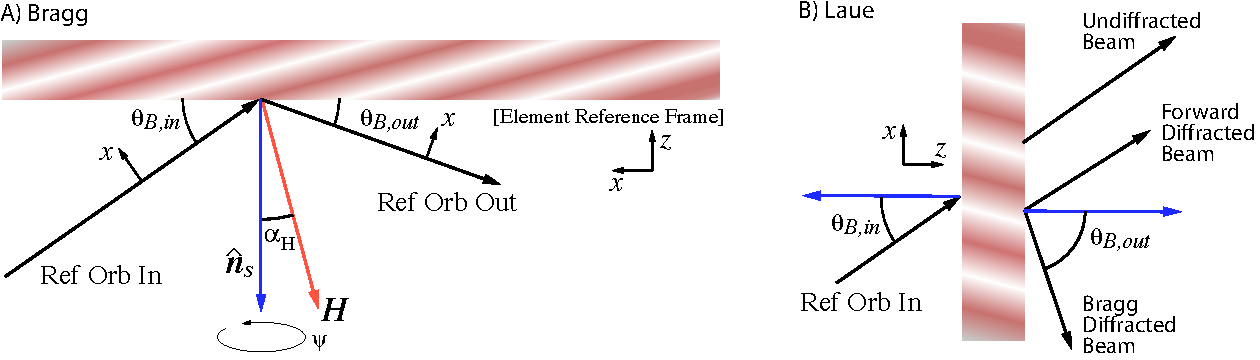
\includegraphics[width=5in]{crystal-ele.pdf}
  \caption[Crystal element geometry.]
{Crystal element geometry.  A) Geometry for Bragg diffraction. The
geometry shown is for \vn{ref_tilt} = 0 (reference trajectory in the
$x$-$z$ plane). The angle $\alpha_H$ (\vn{alpha_angle}) is the angle
of the $\bfH$ vector with respect to the surface normal $\bfhat
n$. For $\psi$ (\vn{psi_angle}) zero, the incoming reference orbit,
the outgoing reference orbit, $\bfhat n$, and $\bfH$ are all
coplanar. B) Geometry for Laue diffraction. In this case there are
three outgoing beams: The Bragg diffracted beam, the forward
diffracted beam, and the undiffracted beam.}
  \label{f:crystal}
\end{figure}

A \vn{crystal} element represents a crystal used for photon diffraction.

General \vn{crystal} attributes are:
\begin{center}
\tt
\begin{tabular}{llll} \toprule
  {\sl Attribute Class}      & Section          & {\sl Attribute Class}      & Section         \\ \midrule
  Aperture limits            & \ref{s:limit}    & Surface Properties         & \ref{s:s.curve} \\ 
  Custom Attributes          & \ref{s:cust.att} & Symplectify                & \ref{s:symp}    \\
  Description strings        & \ref{s:alias}    & Offsets, Pitches \& Tilt   & \ref{s:offset}  \\
  Reference energy           & \ref{s:energy}   & Tracking \& transfer map   & \ref{c:methods} \\
  \bottomrule
\end{tabular}
\end{center}
\toffset
See \sref{s:list.crystal} for a full list of element attributes.

\index{psi_angle}
\index{b_param}\index{bragg_angle}\index{crystal_type}
\index{follow_diffracted_beam}\index{thickness}
Attributes specific to a \vn{crystal} element are:
\begin{example}
  b_param            = <Real>       ! b parameter
  crystal_type       = <String>     ! Crystal material (\sref{s:cryst.list}) and reflection plane.
  psi_angle          = <Real>       ! Rotation of H-vector about the surface normal.
  thickness          = <Real>       ! Thickness of crystal for Laue diffraction.
  ref_orbit_follows  = <which_beam> ! Reference orbit aligned with what outgoing beam?
\end{example}

\index{bragg_angle_in}\index{bragg_angle_out}\index{alpha_angle}
\index{tilt_corr}\index{d_spacing}\index{v_unitcell}\index{l}
\index{ref_wave_length}\index{dbragg_angle_de}
\index{pendellosung_period_sigma}\index{pendellosung_period_pi}
Dependent variables (\sref{s:depend}) specific to a \vn{crystal} element are:
\begin{example}
  alpha_angle                ! Angle of H-vector with respect to the surface normal.
  bragg_angle                ! Nominal Bragg angle at the reference wave length. 
  bragg_angle_in             ! Angle between incoming beam and surface.
  bragg_angle_out            ! Angle between outgoing beam and surface.
  d_spacing                  ! Lattice plane spacing. 
  darwin_width_pi            ! Darwin width for pi polarized light (radians).
  darwin_width_sigma         ! Darwin width for sigma polarized light (radians).
  dbragg_angle_de            ! Variation of the Bragg angle with energy (radians/eV).
  l                          ! Length of reference orbit.
  pendellosung_period_pi     ! Pendellosung period for pi polarized light.
  pendellosung_period_sigma  ! Pendellosung period for sigma polarized light.
  ref_wavelength             ! Reference wavelength (\sref{s:energy}). Dependent attribute (\sref{s:depend}).
  ref_cap_gamma              ! \(\Gamma\) at the reference wavelength.
  tilt_corr                  ! Tilt correction due to a finite psi_angle.
  v_unitcell                 ! Unit cell volume. 
\end{example}

The \vn{crystal_type} attribute defines the crystal material and
diffraction lattice plane. The syntax is \vn{"ZZZ(ijk)"} where \vn{ZZZ}
is the material name and \vn{ijk} are the Miller
indices for the diffraction plane. For example,
\begin{example}
  b_cryst1: crystal, crystal_type = "Si(111)", b_param = -1, ...
\end{example}
The atomic formula is case sensitive so, for example, \vn{"SI(111)"}
is not acceptable. The list of known crystal materials is given in
\sref{s:cryst.list}. Given the \vn{crystal_type}, the spacing between
lattice planes (\vn{d_spacing}), the unit cell volume
(\vn{v_unitcell}), and the structure factor\cite{b:batterman} values
can be computed.

The \vn{b_param} is the standard asymmetry factor
\Begineq
  b = \frac{\sin(\alpha_H + \theta_B)}{\sin(\alpha_H - \theta_B)} 
  \label{batat}
\Endeq
where $\theta_B$ is the Bragg angle (\vn{bragg_angle}) 
\Begineq
  \theta_B = \sin^{-1} \left( \frac{\lambda}{2 \, d} \right)
  \label{tsl2d}
\Endeq
and $\alpha_H$ (\vn{alpha_angle}) is the angle of the reciprocal
lattice $\bfH$ vector with respect to the surface normal as shown in
\fig{f:crystal}A.  If \vn{b_param} is set to -1 then there is
Bragg reflection and \vn{alpha_H} is zero. If \vn{b_param} is set to 1
then there is Laue diffraction again with \vn{alpha_H} zero. With the
orientation shown in \fig{f:crystal}A, \vn{alpha_H} is positive.

The \vn{thickness} parameter is used with Laue diffraction only.

The \vn{ref_orbit_follows} parameter sets how the outgoing reference
orbit is constructed. This is only relevant with Laue diffraction.
The possible settings of this parameter are:
\begin{example}
  bragg_diffracted
  forward_diffracted
  undiffracted
\end{example}
The geometry of this situation is shown in \fig{f:crystal}B. The
reference orbit for the \vn{undiffracted} beam is just a straight line
extension of the incoming reference trajectory. This trajectory is
that trajectory that photons whose energy is far from the Bragg
condition (that is, far from the reference energy) will follow. The
\vn{forward_diffracted} reference orbit is parallel to the
\vn{undiffracted} trajectory and is the trajectory of the forward
diffracted photons whose energy is the reference energy and whose
incoming orbit is on the incoming reference trajectory. Finally, the
\vn{bragg_diffracted} reference orbit is the backward diffracted orbit.

Note: Changing the setting of \vn{ref_orbit_follows} will change the
reference orbit downstream of the crystal which, in turn, will change
the placement all downstream elements.

The value of the element reference orbit length \vn{l} is calculated
by \bmad. \vn{L} will be zero for Bragg diffraction. For Laue
diffraction, \vn{l} will depend upon the crystal \vn{thickness} and
the setting of \vn{ref_orbit_follows}.

If \vn{psi_angle} is zero, the incoming reference orbit, the outgoing
reference orbit, $\bfhat n$ and $\bfH$ are all coplanar. A non-zero
\vn{psi_angle} Rotates the $\bfH$ vector around the $+\bfhat x$ axis
of the \vn{Element Reference Frame} (See \fig{f:crystal}A).

To keep the outgoing reference trajectory independent of the value of
\vn{psi_angle}, the crystal will be automatically tilted by the
appropriate ``tilt correction'' \vn{tilt_corr}. The calculation of
\vn{tilt_corr} is outlined in \sref{s:crystal.trans}. \vn{tilt_corr}
will be zero if \vn{psi_angle} is zero.

The reference trajectory for a Bragg \vn{crystal} is that of a zero
length bend (\sref{s:mirror.coords}) and hence the length (\vn{l})
parameter of a crystal is fixed at zero. The orientation of the
reference trajectory with respect to the crystal surface is specified
by the incoming Bragg angle \vn{bragg_angle_in} ($\theta_{g,in}$) and
outgoing Bragg angle \vn{bragg_angle_out} ($\theta_{g,out}$) as shown
in \fig{f:crystal}A. These angles are computed from the photon
reference energy and the other crystal parameters such that a photon
with the reference energy traveling along the reference trajectory
will be in the center of the Darwin curve (\sref{s:crystal.tracking}).

Notice that due to refraction at the surface, the computed
\vn{bragg_angle} from \Eq{tsl2d} will deviate slightly from the
average of \vn{bragg_angle_in} and \vn{bragg_angle_out}.

The reference trajectory in the global coordinate system
(\sref{s:global}) is determined by the value of the \vn{ref_tilt}
parameter along with the value of \vn{bragg_angle_in} +
\vn{bragg_angle_out}. These bragg angles take into account refraction
so that the reference trajectory downstream of the crystal will be
properly centered with respect to the reference photon. A positive
\vn{bragg_angle_in} + \vn{bragg_angle_out} bends the reference
trajectory in the same direction as a positive \vn{g} for a bend
element. The

A \vn{crystal} may be offset and pitched (\ref{s:offset}). The incoming
local reference coordinates are used for these misalignments. 

When a crystal is bent (\sref{s:s.curve}), the $\bfH$ vector is
assumed follow the surface curvature. That is, it is assumed that the
lattice planes are curved by the bending.

Example:
\begin{example}
  crystal_ele: crystal, crystal_type = 'Si(111)', b_param = -1
\end{example}

The \vn{darwin_width_sigma} and \vn{darwin_width_pi} parameters are
the computed Darwin width, in radians, for sigma and pi polarized
light respectively. Here the Darwin width $d\theta_D$ is defined as
the width at the $\eta = \pm 1$ points
(cf.~Batterman\cite{b:batterman} Eq (32))
\Begineq
  d\theta_D = \frac{2 \, \Gamma \, |P| \, \text{Re} \! \left( [F_H \, F_{\Hbar}]^{1/2} \right)}
                 {|b|^{1/2} \, \sin\theta_{tot}}
\Endeq
where
\begin{example}
  \(\theta_{tot}\) = bragg_angle_in + bragg_angle_out 
\end{example}

The \vn{pendellosung_period_sigma} and \vn{pendellosung_period_pi} are
the pendellosung periods for Laue diffraction. If the crystal is set up for
Bragg diffraction then the values for these parameters will be set to zero.

The \vn{dbragg_angle_de} parameter is the variation in Bragg angle
with respect to the photon energy and is given by the formula
\Begineq
  \frac{d\theta_B}{dE} = -\frac{\lambda}{2 \, d \, E \, \cos( \theta_B )}
\Endeq

%-----------------------------------------------------------------
\section{Custom}
\label{s:custom}
\index{custom|hyperbf}

A \vn{custom} element is an element whose properties are defined
outside of the standard \bmad subroutine library. That is, to use a
custom element, some programmer must write the appropriate custom
routines which are then linked with the \bmad subroutines into a
program. \bmad will call the custom routines at the appropriate time
to do tracking, transfer matrix calculations, etc. See the programmer
who wrote the custom routines for more details! See
\sref{s:custom.ele} on how to write custom routines.

General \vn{custom} attributes are:
\begin{center}
\tt
\begin{tabular}{llll} \toprule
  {\sl Attribute Class}      & Section           & {\sl Attribute Class}      & Section         \\ \midrule
  Aperture limits            & \ref{s:limit}     & Is_on                      & \ref{s:is.on}   \\
  Chamber wall               & \ref{s:wall}      & Length                     & \ref{s:l}       \\
  Custom Attributes          & \ref{s:cust.att}  & Offsets, pitches \& tilt   & \ref{s:offset}  \\
  Description strings        & \ref{s:alias}     & Reference energy           & \ref{s:energy}  \\ 
  Field Maps                 & \ref{s:fieldmap}  & Superposition              & \ref{s:super}   \\
  Fringe fields              & \ref{s:fringe}    & Symplectify                & \ref{s:symp}    \\
  Integration settings       & \ref{s:integ}     & Tracking \& transfer map   & \ref{c:methods} \\ 
  \bottomrule
\end{tabular}
\end{center}
\toffset
See \sref{s:list.custom} for a full list of element attributes.

\index{tracking_method}\index{mat6_calc_method}\index{field_calc}
As an alternative to defining a custom element, standard elements can
be ``customized'' by setting one or more of the following attributes
to \vn{custom}:
\begin{example}
  tracking_method       \sref{s:tkm}
  mat6_calc_method      \sref{s:xfer}
  field_calc            \sref{s:integ}
  aperture_type         \sref{s:limit}
\end{example}

As with a custom element, setting one of these attributes to
\vn{custom} necessitates the use of custom code to implement the
corresponding calculation.

\index{delta_e}
\index{val1,  ..., Val12}
Attributes specific to a \vn{custom} element are
\begin{example}
  val1, ..., val12 = <Real>  ! Custom values 
  delta_e          = <Real>  ! Change in energy.
\end{example}

\vn{delta_e} is the energy gain of the {\it reference} particle
between the starting edge of the element and the ending edge.

Example:
\begin{example}
  c1: custom, l = 3, val4 = 5.6, val12 = 0.9, descrip = 'params.dat'
\end{example}
In this example the \vn{descrip} string is being used to specify a
file that contains parameters for the element.

%-----------------------------------------------------------------
\section{Detector}
\label{s:detector}
\index{detector|hyperbf}

A \vn{detector} element is used to detect particles and X-rays.  A
\vn{detector} is modeled as a grid of pixels which detect particles and x-rays
impinging upon them.

General \vn{detector} element attributes are:
\begin{center}
\tt 
\begin{tabular}{llll} \toprule
  {\sl Attribute Class}      & Section           & {\sl Attribute Class}      & Section         \\ \midrule
  Aperture limits            & \ref{s:limit}     & Offsets, pitches \& tilt   & \ref{s:offset}  \\
  Chamber Wall               & \ref{s:wall}      & Reference energy           & \ref{s:energy}  \\
  Custom Attributes          & \ref{s:cust.att}  & Superposition              & \ref{s:super}   \\
  Description strings        & \ref{s:alias}     & Tracking \& transfer map   & \ref{c:methods} \\
  Detector Geometry          & \ref{s:surf.grid} &                            &                 \\
  \bottomrule
\end{tabular}
\end{center}
\toffset
See \sref{s:list.detector} for a full list of element attributes.

The detector pixels are are arranged in a rectangular grid (\sref{s:surf.grid}). 

\index{aperture_type}
The \vn{aperture_type} (\sref{s:limit}) parameter of a
\vn{detector} will default to \vn{auto} which will set the
aperture limits to define a rectangular aperture that just cover the
clear area of the plate.

Example:
\begin{example}
  det: detector, surface = \{grid = 
          \{ix_bounds = (-4,5), iy_bounds = (-10,10), dr = (0.01, 0.01)\}\}
\end{example}
This example defines a detector with 1~cm x 1~cm pixels.

%-----------------------------------------------------------------
\section{Diffraction_Plate}
\label{s:diff.plate}
\index{diffraction_plate|hyperbf}

A \vn{diffraction_plate} element is a flat surface oriented, more or
less, transversely to a x-ray beam through which photon can travel. A
\vn{diffraction_plate} can be used, for example, to model a Fresnel
zone plate or Young's double slits. A \vn{diffraction_plate} element
is used in places where diffraction effects must be taken into
account. This is in contrast to setting an aperture attribute
(\sref{s:limit} for other elements where diffraction effects are
ignored.

A \vn{diffraction_plate} element is similar to a \vn{mask}
(\sref{s:mask}) element except that with a \vn{mask} element coherent
effects are ignored. Additionally, a \vn{mask} element can be used
with charged particles while a \vn{diffraction_plate} cannot.

General \vn{diffraction_plate} element attributes are:
\begin{center}
\tt 
\begin{tabular}{llll} \toprule
  {\sl Attribute Class}      & Section          & {\sl Attribute Class}      & Section         \\ \midrule
  Aperture limits            & \ref{s:limit}    & Offsets, pitches \& tilt   & \ref{s:offset}   \\ 
  Custom Attributes          & \ref{s:cust.att} & Mask geometry              & \ref{s:wall}    \\
  Description strings        & \ref{s:alias}    & Reference energy           & \ref{s:energy}  \\
  Is_on                      & \ref{s:is.on}    & Tracking \& transfer map   & \ref{c:methods} \\
  \bottomrule
\end{tabular}
\end{center}
\toffset
See \sref{s:list.diffraction.plate} for a full list of element attributes.

\index{mode}\index{field_scale_factor}
Attributes specific to a \vn{diffraction_plate} element are:
\begin{example}
  mode               = <Type>   ! Reflection or transmission
  field_scale_factor = <Real>   ! Factor to scale the photon field
  ref_wavelength                ! Reference wavelength (\sref{s:energy}). Dependent attribute (\sref{s:depend}).
\end{example}

The \vn{mode} switch sets whether X-rays are transmitted through the
\vn{diffraction_plate} or or reflected. Possible values for the
\vn{mode} switch are:
\begin{example}
  reflection
  transmission        ! Default
\end{example}

The geometry of the plate, that is, where the openings (in
transmission mode) or reflection regions are, is defined using the
``wall'' attribute. See (\sref{s:wall}) for more details.

In transmission mode, a \vn{diffraction_plate} is nominally orientated
transversely to the beam. Like all other elements, the
\vn{diffraction_plate} can be reoriented using the element's offsets,
pitches and tilt attributes (\sref{s:offset}).

\index{aperture_type}
The \vn{aperture_type} (\sref{s:limit}) parameter of a
\vn{diffraction_plate} will default to \vn{auto} which will set the
aperture limits to define a rectangular aperture that just cover the
clear area of the plate.

\index{field_scale_factor}
The \vn{field_scale_factor}, if set to a non-zero value (zero is the
default) will be used to scale the field of photons as they pass through
the \vn{diffraction_plate} element:
\begin{example}
  field -> field * field_scale_factor
\end{example}
Scaling is useful since the electric field of photons traveling through a
\vn{diffraction_plate} are renormalized (see \Eqs{eeo4p} and
\eq{eek4p}). This can lead to large variation of the photon field and
can, for example, make visual interpretation of plots of field verses
longitudinal position difficult to interpret. \vn{field_scale_factor}
can be used to keep the field more or less constant.

A \vn{diffraction_plate} that is ``turned off'' (\vn{is_on} attribute
set to False), does not diffract at all and transmits through all
the light incident on it.

Example:
\begin{example}
  fresnel: diffraction_plate, wall = \{...\}
\end{example}

%-----------------------------------------------------------------
\section{Drift}
\label{s:drift}
\index{drift|hyperbf}

A \vn{drift} element is a space free and clear of any fields.

General \vn{drift} attributes are:
\begin{center}
\tt
\begin{tabular}{llll} \toprule
  {\sl Attribute Class}      & Section          & {\sl Attribute Class}      & Section         \\ \midrule
  Aperture limits            & \ref{s:limit}    & Offsets, pitches \& tilt   & \ref{s:offset}  \\
  Custom Attributes          & \ref{s:cust.att} & Reference energy           & \ref{s:energy}  \\ 
  Description strings        & \ref{s:alias}    & Symplectify                & \ref{s:symp}    \\ 
  Length                     & \ref{s:l}        & Tracking \& transfer map   & \ref{c:methods} \\ 
  \bottomrule
\end{tabular}
\end{center}
\toffset
See \sref{s:list.drift} for a full list of element attributes.

Example:
\begin{example}
  d21: drift, l = 4.5
\end{example}

Note: If a chamber wall (\sref{s:wall}) is needed for a field free
space, use a \vn{pipe} element instead of a \vn{drift} [a wall for a
drift is not allowed due to the way drifts are treated with
superposition. That is, drifts ``disappear'' when superimposed
upon. (\sref{s:super})].

%-----------------------------------------------------------------
\section{E_Gun}
\label{s:e.gun}
\index{e_gun|hyperbf}

An \vn{e_gun} element represents an electron gun and encompasses a
region starting from the cathode were the electrons are generated.
General \vn{e_gun} attributes are:
\begin{center}
\tt
\begin{tabular}{llll} \toprule
  {\sl Attribute Class}      & Section           & {\sl Attribute Class}      & Section           \\ \midrule
  Aperture limits            & \ref{s:limit}     & Length                     & \ref{s:l}         \\
  Chamber wall               & \ref{s:wall}      & Mag \& Elec multipoles     & \ref{s:multip}    \\
  Custom attributes          & \ref{s:cust.att}  & Offsets, pitches \& tilt   & \ref{s:offset}    \\ 
  Description strings        & \ref{s:alias}     & Overlapping Fields         & \ref{s:overlap}   \\
  Field autoscaling          & \ref{s:autoscale} & Reference energy           & \ref{s:energy}    \\ 
  Hkick \& Vkick             & \ref{s:kick}      & Symplectify                & \ref{s:symp}      \\
  Integration settings       & \ref{s:integ}     & Field Maps                 & \ref{s:fieldmap}  \\
  Is_on                      & \ref{s:is.on}     & Tracking \& transfer map   & \ref{c:methods}   \\ 
  \bottomrule
\end{tabular}
\end{center}
\toffset
See \sref{s:list.e.gun} for a full list of element attributes.

The attributes specific to an \vn{e_gun} are 
\index{voltage}\index{voltage_err}
\index{gradient}\index{gradient_err}
\begin{example}
  gradient       = <Real>    ! Gradient.
  gradient_err   = <Real>    ! Gradient error.
  phi0           = <Real>    ! Phase (rad/2\(\pi\)) of the reference particle with 
                             !   respect to the RF. phi0 = 0 is on crest.
  phi0_err       = <Real>    ! Phase error (rad/2\(\pi\))
  rf_frequency   = <Real>    ! Frequency of the RF field.
  voltage        = <Real>    ! Voltage. Dependent attribute (\sref{s:depend}). 
  voltage_err    = <Real>    ! Voltage error. Dependent attribute (\sref{s:depend}). 
\end{example}

The \vn{voltage} is simply related to the \vn{gradient} via the element length \vn{l}:
\begin{example}
  voltage = gradient * l
\end{example}
If the \vn{voltage} is set to a non-zero value, the length \vn{l} must also be non-zero to
keep the gradient finite.  A particle with the charge as the reference particle will have
a positive energy gain if the \vn{voltage} and \vn{gradient} are positive and vice versa.

\index{phi0_autoscale}\vn{field_autoscale}
The \vn{voltage} and \vn{gradient} are scaled by \vn{field_autoscale} and, if there is a
finite \vn{rf_frequency}, the phase of the frequency is shifted by \vn{phi0_autoscale} as
discussed in Section~\sref{s:autoscale}. Autoscaling can be toggled on/off by using the
\vn{autoscale_phase} and \vn{autoscale_amplitude} toggles.

An \vn{e_gun} may either be DC if the \vn{rf_frequency} component is zero of AC if
not. For an AC \vn{e_gun}, the phase of the \vn{e_gun}, The phase $\phi_{\text{ref}}$
is 
\begin{example} 
  \(\phi_{\text{ref}}\) = phi0 + phi0_err + phi0_autoscale 
\end{example}

\index{marker}\index{null_ele}
Electrons generated at the cathode can have zero initial momentum and
this presents a special problem (\sref{s:energy}). As a result, the
use of \vn{e_gun} elements are restricted and they can only be used in
a ``linear'' (non-recirculating) lattice branch. Only one \vn{e_gun}
can be present in a lattice branch and, if it is present, it must be,
except for possibly \vn{marker} or \vn{null_ele} elements, the first
element in any branch.
 
Note: In order to be able to avoid problems with a zero reference
momentum at the beginning of the \vn{e_gun}, the reference momentum
and energy associated with an \vn{e_gun} element is calculated as
outlined in Section~\sref{s:energy}. Additionally, the reference
momentum at the exit end of the \vn{e_gun}, that is \vn{p0c}, must be
non-zero. Thus, for example, if \vn{p0c} is zero at the start of the
lattice, the \vn{e_gun} voltage must be non-zero. 

Additionally, in order to be able to avoid problems with a zero reference momentum at the
beginning of the \vn{e_gun}, absolute time tracking (\sref{s:rf.time}) is always used in
an \vn{e_gun} element independent of the setting of \vn{parameter[absolute_time_tracking]}
(\sref{s:param}).

Note: The default \vn{tracking_method} (\sref{s:tkm}) setting for an
\vn{e_gun} is \vn{time_runge_kutta} and the default
\vn{mat6_calc_method} is \vn{tracking}.

In this example the field of an e_gun is given by a grid of field
values (\sref{s:grid.field}):
\begin{example}
  apex: e_gun, l = 0.23, field_calc = fieldmap, rf_frequency = 187e6, 
                grid_field = call::apex_gun_grid.bmad
\end{example}
with the file \vn{apex_gun_grid.bmad} being:
\begin{example}
  \{
    m = 0, harmonic = 1,
    master_scale = voltage,
    geometry = rotationally_symmetric_rz,
    r0 = (0, 0),
    dr = (0.001, 0.001),
    pt(0,0) = ( (0, 0), (0, 0), (1, 0),  (0, 0), (0, 0), (0, 0)),
    pt(0,1) = ( (0, 0), (0, 0), (0.99, 0),  (0, 0), (0, 0), (0, 0)),
    ... \}
\end{example}

%-----------------------------------------------------------------
\section{ELseparator}
\label{s:elsep}
\index{elseparator|hyperbf}

An \vn{elseparator} is an electrostatic separator.

General \vn{elseparator} attributes are:
\begin{center}
\tt
\begin{tabular}{llll} \toprule
  {\sl Attribute Class}      & Section           & {\sl Attribute Class}      & Section          \\ \midrule
  Aperture limits            & \ref{s:limit}     & Mag \& Elec multipoles     & \ref{s:multip}   \\
  Chamber wall               & \ref{s:wall}      & Offsets, pitches \& tilt   & \ref{s:offset}   \\
  Custom Attributes          & \ref{s:cust.att}  & Overlapping Fields         & \ref{s:overlap}  \\
  Description strings        & \ref{s:alias}     & Reference energy           & \ref{s:energy}   \\ 
  Fringe Fields              & \ref{s:fringe}    & Superposition              & \ref{s:super}    \\
  Hkick \& Vkick             & \ref{s:kick}      & Symplectify                & \ref{s:symp}     \\
  Integration settings       & \ref{s:integ}     & Field Maps                 & \ref{s:fieldmap} \\  
  Is_on                      & \ref{s:is.on}     & Tracking \& transfer map   & \ref{c:methods}  \\ 
  Length                     & \ref{s:l}         &                            &                  \\
  \bottomrule
\end{tabular}
\end{center}
\toffset
See \sref{s:list.elseparator} for a full list of element attributes.

\index{gap}
\index{e_field}
\index{voltage}
Attributes specific to an \vn{elseparator} element are:
\begin{example}
  gap = <Real> ! Distance between electrodes
  voltage      ! Voltage between electrodes. This is a settable dependent variable (\sref{s:depend}).
  e_field      ! Electric field. This is a settable dependent variable (\sref{s:depend}).
\end{example}

\index{hkick}
\index{vkick}
For an \vn{elseparator}, the kick for a positively charged particle, with the magnitude of
the charge that is the same as the reference particle (set by \vn{parameter[particle]}
\sref{s:param}), is determined by \vn{hkick} and \vn{vkick}. The kick for a negatively
charged particle is opposite this. The \vn{gap} for an \vn{Elseparator} is used to compute
the voltage for a given kick
\begin{example}
  e_field (V/m) = sqrt(hkick^2 + vkick^2) * P0 * c_light / L
  voltage (V) = e_field * gap
\end{example}

Example:
\begin{example}
  h_sep: elsep, l = 4.5, hkick = 0.003, gap = 0.11
\end{example}

%-----------------------------------------------------------------
\section{EM_Field}
\label{s:em.field}
\index{em_field|hyperbf}

An \vn{em_field} element can contain general electro-magnetic (EM)
fields. Both AC and DC fields are accommodated.  General \vn{em_field}
attributes are:
\begin{center}
\tt
\begin{tabular}{llll} \toprule
  {\sl Attribute Class}      & Section           & {\sl Attribute Class}      & Section         \\ \midrule
  Aperture limits            & \ref{s:limit}     & Is_on                      & \ref{s:is.on}   \\
  Chamber wall               & \ref{s:wall}      & Length                     & \ref{s:l}       \\ 
  Custom Attributes          & \ref{s:cust.att}  & Offsets, pitches \& tilt   & \ref{s:offset}  \\
  Description strings        & \ref{s:alias}     & Reference energy           & \ref{s:energy}  \\
  Field Maps                 & \ref{s:fieldmap}  & Superposition              & \ref{s:super}   \\
  Hkick \& Vkick             & \ref{s:kick}      & Symplectify                & \ref{s:symp}    \\
  Integration settings       & \ref{s:integ}     & Tracking \& transfer map   & \ref{c:methods} \\
  \bottomrule
\end{tabular}
\end{center}
\toffset
See \sref{s:list.em.field} for a full list of element attributes.

\index{constant_ref_energy}
Attributes specific to an \vn{em_field} element are:
\begin{example}
  constant_ref_energy = <Logical> ! Does the element have a constant reference energy? Default = True.
\end{example}

If the \vn{constant_ref_energy} logical is set to \vn{True} (the default), the reference energy
(\sref{s:ref.energy}) at the exit end of the element is set equal to the entrance end referece
energy. This is the same behavior for most other elements. If the \vn{constant_ref_energy} logical
is set to \vn{False}, the reference energy at the exit end is calculated like it is in a
\vn{lcavity} or \vn{e_gun} element.

Note: \vn{em_field} elements will be created when elements are superimposed (\sref{s:super}) and there is
no other suitable element class.

%-----------------------------------------------------------------
\section{Fiducial}
\label{s:fiducial}
\index{fiducial|hyperbf}

A \vn{fiducial} element is used to fix the position and orientation of the reference orbit within
the global coordinate system at the location of the \vn{fiducial} element. A \vn{fiducial} element
will affect the global floor coordinates (\sref{s:global}) of elements both upstream and downstream
of the fiducial element.

Other elements that are used to shift the lattice in the global coordinate frame are
\vn{floor_shift} (\sref{s:floor.ele}) and \vn{patch} (\sref{s:patch}).

General \vn{fiducial} element attributes are:
\begin{center}
\tt
\begin{tabular}{llll} \toprule
  {\sl Attribute Class}      & Section           & {\sl Attribute Class}      & Section         \\ \midrule
  Aperture limits            & \ref{s:limit}     & Reference energy           & \ref{s:energy}  \\
  Custom Attributes          & \ref{s:cust.att}  & Superposition              & \ref{s:super}   \\
  Description strings        & \ref{s:alias}     & Tracking \& transfer map   & \ref{c:methods} \\ 
  \bottomrule
\end{tabular}
\end{center}
\toffset
See \sref{s:list.fiducial} for a full list of element attributes.

\index{origin_ele}\index{origin_ele_ref_pt}
\index{x_origin}\index{y_origin}
\index{z_origin}\index{theta_origin}
\index{phi_origin}\index{psi_origin}
Attributes specific to a \vn{fiducial} elements are:
\begin{example}
  origin_ele        = <Name>     ! Reference element.
  origin_ele_ref_pt = <location> ! Reference pt on reference ele.
  dx_origin         = <Real>     ! x-position offset
  dy_origin         = <Real>     ! y-position offset
  dz_origin         = <Real>     ! z-position offset
  dtheta_origin     = <Real>     ! orientation angle offset.
  dphi_origin       = <Real>     ! orientation angle offset.
  dpsi_origin       = <Real>     ! orientation angle offset.
\end{example}

For tracking purposes, the \vn{fiducial} element is considered to be a
zero length marker. That is, the transfer map through a \vn{fiducial}
element is the unit map.

A \vn{fiducial} element sets the global floor coordinates (\sref{s:global}) of itself and of the
elements, both upstream and downstream, around it. This can be thought of as a two step process. The
first step is to determine the global coordinates of the \vn{fiducial} element itself, and the
second step is to shift the coordinates of the elements around it. That is, shifting the position
of a \vn{fiducial} element shifts the lattice elements around it as one solid body.

The floor coordinates of the \vn{fiducial} element are determined
starting with an \vn{origin_ele} element. If \vn{origin_ele} is not
specified, the origin of the global coordinates (\sref{s:global} is
used. If the \vn{origin_ele} has a finite length, the reference point
may be chosen using the \vn{origin_ele_ref_pt} attribute which
may be set to one of
\begin{example}
  entrance_end
  center         ! Default
  exit_end
\end{example}

Once the origin reference position is determined, the reference
position of the \vn{fiducial} element is calculated using the offset
attributes 
\begin{example}
  [dx_origin,  dy_origin,  dz_origin]
  [dtheta_origin,  dphi_origin,  dpsi_origin]
\end{example}
The transformation between origin and fiducial positions is given in
\sref{s:patch.coords}.

\index{flexible patch}\index{patch}
Once the position of the \vn{fiducial} element is calculated, all
elements of the lattice branch the \vn{fiducial} element is contained
in, {\em both} the upstream and downstream elements, are shifted so
that everything is consistent. That is, the \vn{fiducial} element
orients the entire lattice branch. The exception here is that if there
are \vn{flexible} \vn{patch} elements (\sref{s:patch}) in the lattice
branch, the \vn{fiducial} element will only determine the positions up
to the \vn{flexible} \vn{patch} element. 

Example: A lattice branch with elements 0 through 103 has a
\vn{fiducial} element at position 34 and a \vn{flexible} \vn{patch} at
position 67. In this case the \vn{fiducial} element will determine the
reference orbit for elements 0 through 66.

Rules: 
  \begin{itemize}
  \item
If an \vn{origin_ele} is specified, the position of this element must
to calculated before the the position of the \vn{fiducial} element is
calculated (\sref{s:ref}). This means, the \vn{origin_ele} must be in
a prior lattice branch from the branch the \vn{fiducial} element is in
or the \vn{origin_ele} in the same branch as the \vn{fiducial} element
but is positioned upstream from the \vn{fiducial} element and there is
a \vn{flexible} \vn{patch} in between the two elements.
  \item
If a \vn{fiducial} element affects the position of element 0 in the
lattice branch (that is, there are no flexible \vn{patch} elements
in between), any positioning of element 0 via \vn{beginning} or
\vn{line parameter} statements (\sref{s:beginning}) are ignored.
  \item
\vn{Fiducial} elements must not over constrain the lattice geometry.
For example, two \vn{fiducial} elements may not appear in the same
lattice branch unless separated by a \vn{flexible} \vn{patch}. 

Another example is that if there are no flexible \vn{patch} elements
in the lattice, and if branch \vn{A} has a \vn{branch} element
connecting to branch \vn{B}, the geometry of branch \vn{A} will be
calculated first and the geometry of branch \vn{B} can then be
calculated from the known coordinates of the \vn{fork} element. If
branch \vn{B} contains a \vn{fiducial} element then this is an error
since the coordinate calculation never backtracks to recalculate the
coordinates of the elements of a branch once the calculation has
finished with that branch.
  \end{itemize}

Example:
\begin{example}
  f1: fiducial, origin_ele = mark1, x_offset = 0.04
\end{example}
See \sref{s:ex.collide} for an example where a fiducial element is
used to position the second ring in a dual ring colliding beam 
machine.

%-----------------------------------------------------------------
\section{Floor_Shift}
\label{s:floor.ele}
\index{floor_shift|hyperbf}

A \vn{floor_shift} element shifts the reference orbit in the global coordinate system without
affecting particle tracking. That is, in terms of tracking, a \vn{floor_shift} element is equivalent
to a \vn{marker} (\sref{s:mark}) element. 

Also see \vn{patch} (\sref{s:patch}) and \vn{fiducial} (\sref{s:fiducial}) elements.

General \vn{floor_shift} element attributes are:
\begin{center}
\tt
\begin{tabular}{llll} \toprule
  {\sl Attribute Class}      & Section           & {\sl Attribute Class}      & Section         \\ \midrule
  Aperture limits            & \ref{s:limit}     & Reference energy           & \ref{s:energy}  \\
  Custom Attributes          & \ref{s:cust.att}  & Superposition              & \ref{s:super}   \\
  Description strings        & \ref{s:alias}     & Tracking \& transfer map   & \ref{c:methods} \\
  Length                     & \ref{s:l}         &                            &                 \\
  \bottomrule
\end{tabular}
\end{center}
\toffset
See \sref{s:list.floor.shift} for a full list of element attributes.

\index{l}\index{x_offset}\index{y_offset}\index{z_offset}
\index{tilt}\index{x_pitch}\index{y_pitch}
\index{origin_ele}\index{origin_ele_ref_pt}
Attributes specific to a \vn{floor_shift} elements are:
\begin{example}
  l                 = <Real>     ! Length
  x_offset          = <Real>     ! x offset from origin point.
  y_offset          = <Real>     ! y offset from origin point.
  z_offset          = <Real>     ! z offset from origin point.
  x_pitch           = <Real>     ! rotation of the reference coords.
  y_pitch           = <Real>     ! rotation of the reference coords.
  tilt              = <Real>     ! rotation of the reference coords.
  origin_ele        = <Name>     ! Reference element.
  origin_ele_ref_pt = <location> ! Reference pt on the reference ele.
\end{example}

The \vn{floor_shift} element sets the reference orbit at the exit end of the \vn{floor_shift}
element as follows: Start with the the reference orbit at the \vn{origin_ele} reference point (see
below). This coordinate system is shifted using the offset, pitch and tilt parameters of the
\vn{floor_shift} element. The shifted coordinate system is used as the coordinate system at the exit
end of the \vn{floor_shift} element. The reference position transformation through a
\vn{floor_shift} element is given in Section~\sref{s:patch.coords}. In this respect, the \vn{floor_shift}
element is similar to the \vn{fiducial} element. The difference being that the \vn{fiducial} element affects
the global floor coordinates of elements both upstream and downstream of the \vn{fiducial} element while a
\vn{floor_shift} element only affects the floor position of elements downstream from it.
 
Like a \vn{fiducial} element, the transfer map through a \vn{floor_shift} element will be the
unit map. That is, the phase space coordinates of a particle will not change when tracking through a
\vn{floor_shift} element. 

The \vn{l} attribute can be used to adjust the longitudinal $s$ position.

The \vn{floor_shift} element can be used, for example, to restore the
correct global geometry when a section of the lattice is represented by, say,
a \vn{taylor} type element.

If an \vn{origin_ele} is specified, the position of this element must to calculated before the the
position of the \vn{fiducial} element is calculated. See the discussion of the \vn{origin_ele} for
\vn{fiducial} elements (\sref{s:fiducial}).  Notice that if the \vn{origin_ele} is specified, and is
different from the element upstream from the \vn{floor_shift} element, the coordinates at the exit
end of the \vn{floor_shift} element is independent of the coordinates of the upstream element.

If the \vn{origin_ele} has a finite length, the reference point may be chosen using the
\vn{origin_ele_ref_pt} attribute which may be set to one of
\begin{example}
  entrance_end
  center
  exit_end         ! Default
\end{example}


PTC does not have an analogous element for the \vn{Floor_shift}
element. When converting to PTC, a \vn{floor_shift} element will be treated
as a \vn{marker} element.

Example: 
\begin{example}
  floor: floor_shift, z_offset = 3.2
\end{example}
This offsets the element after the \vn{floor_shift} 3.2 meters from the previous
element.

%-----------------------------------------------------------------
\section{Fork and Photon_Fork}
\label{s:fork}
\index{fork|hyperbf}
\index{photon_fork|hyperbf}

\begin{figure}[tb]
  \centering
  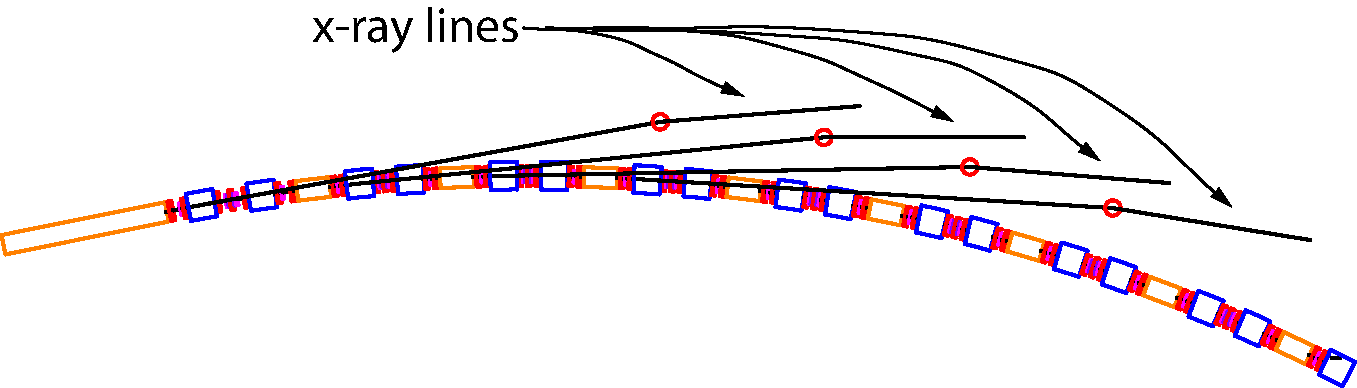
\includegraphics[width=5in]{x-fork.pdf}
  \caption[Example with photon_fork elements.]
  {
Example use of \vn{photon_fork} elements showing four X-ray lines (branches)
attached to a machine.
  }
  \label{f:x.fork}
\end{figure}

A \vn{fork} or \vn{photon_fork} element marks the start of an
alternative \vn{branch} for the beam (or X-rays or other
particles generated by the beam) to follow. 

Collectively \vn{fork} and \vn{photon_fork} elements are called
forking elements. An example geometry is shown in \fig{f:x.fork}.  The
\vn{branch} containing a forking element is called the ``\vn{base}
\vn{branch}''. The \vn{branch} that the forking element points to is
called the ``\vn{target} \vn{branch}''. 

The only difference between \vn{fork} and \vn{photon_fork} is that the
default particle type for the target branch forked from a \vn{fork}
element is the same particle type as the base branch. The default
particle type for the target branch from a \vn{photon_fork} element is
a photon. The actual particle associated with a branch can be set by
setting the \vn{particle} attribute of the forking element.

General \vn{fork} and \vn{photon_fork} attributes are:
\begin{center}
\tt
\begin{tabular}{llll} \toprule
  {\sl Attribute Class}      & Section           & {\sl Attribute Class}      & Section         \\ \midrule
  Aperture limits            & \ref{s:limit}     & Length                     & \ref{s:l}       \\
  Chamber wall               & \ref{s:wall}      & Reference energy           & \ref{s:energy}  \\ 
  Custom Attributes          & \ref{s:cust.att}  & Superposition              & \ref{s:super}   \\
  Description strings        & \ref{s:alias}     & Tracking \& transfer map   & \ref{c:methods} \\ 
  Is_on                      & \ref{s:is.on}     &                            &                 \\
  \bottomrule
\end{tabular}
\end{center}
\toffset
See \sref{s:list.fork} for a full list of element attributes.

Attributes specific to \vn{fork} and \vn{photon_fork} elements are:
\begin{example}
  direction    = <+/- 1>      ! Fork for forward or backwards propagating particles?
  to_line      = <LineName>   ! What line to fork to.
  to_element   = <ElementID>  ! What element to attach to in the line being forked to.
  new_branch   = <T/F>        ! Make a new branch from the to_line? Default = True.
\end{example}

\index{patch}
Branch lines can themselves have forking elements. A branch line
always starts out tangential to the line it is branching from.  A
\vn{patch} element (\sref{s:patch}) can be used to reorient the
reference orbit as needed. Example:
\begin{example}
  from_line: line = (... A, PB, B, ...)  ! Defines base branch
  pb: photon_fork, to_line = x_line
  x_line: line = (X_PATCH, X1, X2, ...)           ! Defines target branch
  x_patch: patch, x_offset = 0.01
  use, from_line
\end{example}
In this example, a photon generated at the fork element \vn{PB} with
$x = 0$ with respect to the \vn{from_line} reference orbit through
\vn{PB} will, when transferred to the \vn{x_line}, and propagated
through \vn{X_PATCH}, have an initial value for $x$ of $-0.01$.

Forking elements have zero length and, like \vn{marker} elements, the
position of a particle tracked through a forking element does not change.

Forking elements do not have orientational attributes like
\vn{x_pitch} and \vn{tilt} (\ref{s:offset}). If the orientation of the
target branch needs to be modified, this can be accomplished using a
\vn{patch} element at the beginning of the line.

\index{is_on}
The \vn{is_on} attribute, while provided for use by a program, is
ignored by \bmad proper.

If the reference orbit needs to be shifted when forking from one ring
to another ring, a patch can be placed in a separate ``transfer'' line
to isolate it from the branches defining the rings. Example:
\begin{example}
  ring1: line = (... A, F1, B, ...)     ! First ring
  x_line: line = (X_F1, X_PATCH, X_F2)  ! ``Transfer'' line
  ring2: line = (... C, F2, D, ...)     ! Second ring
  use, ring1

  f1: fork, to_line = x_line
  f2: fork, to_line = x_line, direction = -1
  x_patch: patch, x_offset = ...
  x_f1: fork, to_line = ring1, to_element = f1, direction = -1
  x_f2: fork, to_line = ring2, to_element = f2
\end{example}
Here the \vn{fork} \vn{F1} in \vn{ring1} forks to \vn{x_line} which
in turn forks to \vn{ring2}.

The above example also illustrates how to connect machines for particles going in the
reverse direction. In this case, \vn{ring2} has a \vn{fork} element \vn{f2} back through
\vn{x_line} and then to \vn{ring1} via the \vn{x_f1} fork. Notice that both \vn{f2} and
\vn{x_f2} have their \vn{direction} attribute set to -1 to indicate that the fork is
appropriate for particles propagating in the -$s$ direction.  Additionally, since \vn{f2}
has \vn{direction} set to -1, it will, by default, connect to the downstream end of the
\vn{x_line}. The default setting of \vn{direction} is 1. 

It is important to note that the setting of \vn{direction} does not change the placement
of elements in the forked line. That is, the global position (\sref{s:global}) of any
element is unaffected by the setting of \vn{direction}. To shift the the global position
of a forked line, \vn{patch} elements must be used.

\index{beginning_ele}\index{fiducial}\index{fork}\index{photon_fork}
\index{marker}\index{to_element}
The \vn{to_element} attribute for a forking element is used to
designate the element of the target branch that the forking element
connects to. To keep things conceptually simple, the \vn{to_element}
must be a ``marker-like'' element which has zero length and unit
transfer matrix. Possible \vn{to_element} types are:
\begin{example}
  beginning_ele
  fiducial
  fork and photon_fork
  marker
\end{example}
When the \vn{to_element} is not specified, the default is to connect
to the beginning of the target branch if \vn{direction} is 1 and to
connect to the end of the target branch if \vn{direction} is -1. In
this case, there is never a problem connecting to the beginning of the
target branch since all branches have a \vn{beginning_ele} element at
the beginning. When connecting to the end of the target branch the
last element in the target branch must be a marker-like element. Note
that, by default, a marker element is placed at the end of all
branches (\sref{s:branch.construct})

The reference energy of a target branch line, needs to be set using
line parameter statements (\sref{s:beginning}). The default reference
particle type of a branch line will be a \vn{photon} is using a
\vn{photon_fork} or will be the same type of particle as the base
branch if a \vn{fork} element is used.

Example showing an injection line branching to a ring which, in turn,
branches to two x-ray lines:
\begin{example}
  inj: line = (..., br_ele, ...)            ! Define the injection line
  use, inj                                  ! Injection line is the root
  br_ele: fork, to_line = ring              ! Fork element to ring
  ring: line = (..., x_br, ..., x_br, ...)  ! Define the ring
  x_br: photon_fork, to_line = x_line       ! Fork element to x-ray line
  x_line: line = (...)                      ! Define the x-ray line
  x_line[E_tot] = 1e3
\end{example}

The \vn{new_branch} attribute is, by default, \vn{True} which means
that the lattice branch created out of the \vn{to_line} line is
distinct from other lattice branches of the same name. Thus, in the
above example, the two lattice branches made from the \vn{x_line} will
be distinct. If \vn{new_branch} is set to \vn{False}, a new lattice
branch will not be created if a lattice branch created from the same
line already exists. This is useful, for example, when a chicane line
branches off from the main line and then branches back to it.

When a lattice is expanded (\sref{s:expand}), the branches defined by
the \vn{use} statement (\sref{s:use}) are searched for fork elements
that branch to new target branches. If found, the appropriate branches are
instantiated and the process repeated until there are no more branches
to be instantiated. This process does {\em not} go in reverse. That is
the lines defined in a lattice file are not searched for fork elements
that have target instantiated branches. For example, if, in the above example,
the use statement was:
\begin{example}
  use, x_line
\end{example}
then only the \vn{x_line} would be instantiated and the lines \vn{inj} and
\vn{ring} would be ignored.

%-----------------------------------------------------------------
\section{Girder}
\label{s:girder}
\index{girder|hyperbf}

\begin{figure}[t]
  \centering
  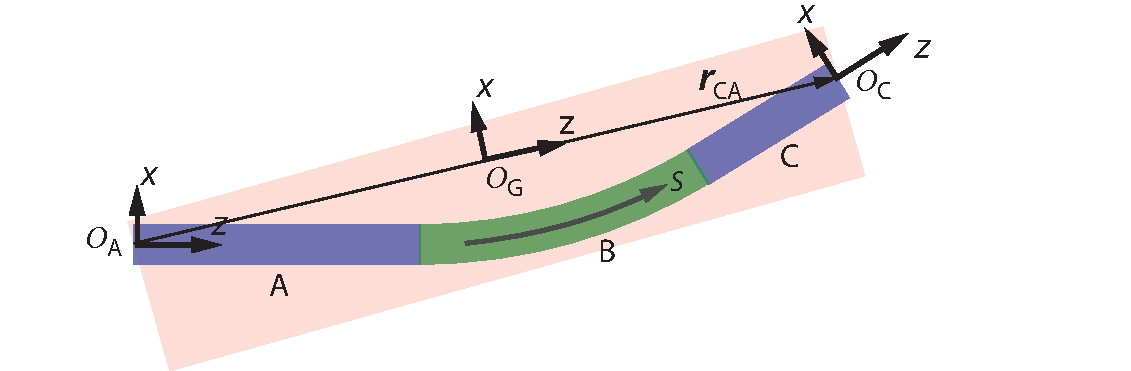
\includegraphics{girder.pdf}
  \caption[Girder example.] {
Girder supporting three elements labeled \vn{A}, \vn{B}, and \vn{C}.
$\calO_A$ is the reference frame at the upstream end of element \vn{A}
(\sref{s:ref.construct}), $\calO_C$ is the reference frame at the
downstream end of element \vn{C}, and $\calO_G$ is the default
\vn{origin} reference frame of the girder. $r_{CA}$ is the vector from
$\calO_A$ to $\calO_C$. The length \vn{l} of the girder is the
difference in $s$ between points $\calO_C$ and $\calO_A$.
  }
  \label{f:girder}
\end{figure}

A \vn{girder} is a support structure that orients the elements that
are attached to it in space. A girder can be used to simulate any
rigid support structure and there are no restrictions on how the lattice
elements that are supported are oriented with respect to one another.
Thus, for example, optical tables can be simulated.

General \vn{girder} attributes are:
\begin{center}
\tt
\begin{tabular}{llll} \toprule
  {\sl Attribute Class}      & Section           & {\sl Attribute Class}      & Section         \\ \midrule
  Custom Attributes          & \ref{s:cust.att}  & Length                     & \ref{s:l}       \\
  Description strings        & \ref{s:alias}     & Offsets, pitches \& tilt   & \ref{s:offset}  \\ 
  Is_on                      & \ref{s:is.on}     &                            &                 \\
  \bottomrule
\end{tabular}
\end{center}
\toffset
See \sref{s:list.girder} for a full list of element attributes.

Attributes specific to a \vn{girder} are:
\index{origin_ele}\index{origin_ele_ref_pt}
\index{x_origin}\index{y_origin}
\index{z_origin}\index{theta_origin}
\index{phi_origin}\index{psi_origin}
Attributes specific to a \vn{floor_shift} elements are:
\begin{example}
  girder = \{<List>\}   ! List of elements on the Girder
  origin_ele        = <Name>     ! Reference element.
  origin_ele_ref_pt = <location> ! Reference pt on reference ele.
  dx_origin         = <Real>     ! x-position offset
  dy_origin         = <Real>     ! y-position offset
  dz_origin         = <Real>     ! z-position offset
  dtheta_origin     = <Real>     ! orientation angle offset.
  dphi_origin       = <Real>     ! orientation angle offset.
  dpsi_origin       = <Real>     ! orientation angle offset.
  l                 ! Girder ``Length'' (\ref{s:l}). Dependent attribute (\sref{s:depend}).
\end{example}

A simple example of a girder is shown in \fig{f:girder}. Here a girder supports three
elements labeled \vn{A}, \vn{B}, and \vn{C} where \vn{B} is a bend so the geometry is
nonlinear. Such a girder may specified in the lattice file like:
\begin{example}
  g1: girder = \{A, B, C\}
\end{example}

The \vn{girder} statement can take one of two forms:
\begin{example}
  <element_name>: GIRDER = \{<ele1>, <ele2>, ..., <eleN>\}, ... 
\end{example}
or
\begin{example}
  <element_name>: GIRDER = \{<ele_start>:<ele_end>\}, ... 
\end{example}

With the first form, a \vn{girder} element will be created for each section of the lattice where there is a
``consecutive'' sequence of ``slave'' elements \vn{<ele1>} through \vn{<eleN>}.  This
section of the lattice from \vn{<ele1>} through \vn{<eleN>} is called the ``girder support
region''.  ``Consecutive'' here means there are no other elements in the girder support
region except for possibly \vn{drift} and/or \vn{marker} elements.  \vn{Drift} elements
cannot be controlled by a girder but may appear in the girder slave list. If a \vn{drift}
does appear in the slave list, only \vn{marker} elements, but not \vn{dirft} elements will
be ignored when determining if elements are consecutive. Note: If a drift-like element is
desired to be supported by a \vn{girder}, use a \vn{pipe} element instead. \vn{Marker}
elements present in a girder support region, but not mentioned in the girder slave list,
are simply ignored.

The second form of a \vn{girder} statment specifies the first and last elements in the 
sequence of elements to be supported. Everything in between except \vn{drift} elements will
be supported by the \vn{girder}.

Wild card characters (\sref{s:lat.attribs}) can be used in any element
name in the girder slave list. Additionally, beam line names
(\sref{s:lines.wo.arg}) can be used. In this case, any \vn{drift} elements
within a beam line will be ignored.

A lattice element may have at most one \vn{girder} supporting
it. However, a \vn{girder} can be supported by another \vn{girder}
which in turn can be supported by a third \vn{girder}, etc. Girders
that support other girders must be defined in the lattice file after
the supported girders are defined. Example:
\begin{example}
  g1: girder = \{A, B, C\}
  g2: girder = \{g1\}      ! g2 must come after g1!
\end{example}

A \vn{girder} may not directly support \vn{multipass_slave}
(\sref{s:multipass}) or \vn{super_slave} (\sref{s:super})
elements. Rather, a \vn{girder} may support the corresponding lord
elements.

The reference frame from which the girder's offset, pitch, and tilt
attributes (\sref{s:offset}) are measured is constructed as follows: A
reference frame, called the ``\vn{origin}'' reference frame may be
defined using the attributes \vn{origin_ele} and
\vn{origin_ele_ref_pt} which constructs the girder's
\vn{origin} frame to be coincident with the reference frame of another
element. Example:
\begin{example}
  g2: girder = \{...\}, origin_ele = Q, origin_ele_ref_pt = entrance_end
\end{example}
In this example, girder \vn{g2} has an \vn{origin} reference frame
coincident with the entrance end frame of an element named
\vn{Q}. Valid values are
\begin{example}
  entrance_end
  center        ! Default
  exit_end
\end{example}
For \vn{crystal}, \vn{mirror}, and \vn{multilayer_mirror} elements,
setting \vn{origin_ele_ref_pt} to \vn{center} results in the reference
frame being the frame of the surface (cf.~\fig{f:surface}).

If \vn{origin_ele} is not given, the default \vn{origin} frame is
used. The default \vn{origin} frame is constructed as follows:
Let $\calO_A$ be the reference frame of the upstream end of
the first element in the list of supported elements. In this example
it is the upstream end of element \vn{A} as shown in the figure. Let
$\calO_C$ be the downstream end of the last element in the list of
supported elements. In this example this is the downstream end of
element \vn{C}. The origin of the \vn{girder}'s reference frame,
marked $\calO_G$ in the figure, will be half way along the vector
$r_{CA}$ from the origin of $\calO_A$ to the origin of $\calO_B$.  The
orientation of $\calO_G$ is constructed by rotating the $\calO_A$
coordinate system along an axis in $\calO_A$'s $x$-$y$ plane such that
$\calO_A$'s $z$ axis ends up parallel with $r_{CA}$. In the example
above, the rotation axis will be along $\calO_A$'s $y$-axis.

Once the \vn{origin} reference frame is established, the reference
frame of the girder can be offset
from the \vn{origin} frame using the parameters
\begin{example}
  dx_origin    dtheta_origin
  dy_origin    dphi_origin
  dz_origin    dpsi_origin
\end{example} 
The orientation of the \vn{girder}'s reference frame from the \vn{origin}
frame is given in \sref{s:patch.coords}. Example:
\begin{example}
  g3: girder = \{ ... \}, dx_origin = 0.03
\end{example}
This offsets girder \vn{g3}'s reference frame 3~cm horizontally from
the default \vn{origin} frame. If no offsets are given, the
\vn{origin} frame is the same as the girder's reference frame.

The length \vn{l} of a girder, which is not used in any calculations,
is a dependent attribute computed by \bmad and set equal to the $s$
path length between points $\calO_C$ and $\calO_A$.

\index{x_offset}\index{y_offset}\index{x_pitch}\index{y_pitch}\index{tilt}
The physical orientation of the girder with respect to it's reference
frame is, like other elements, determined by the offset, pitch and
tilt orientation attributes as outlined in \sref{s:offset} and
\sref{s:patch.coords}.  When a girder is shifted in space, the elements
it supports are also shifted.  In this case, the orientation
attributes (\vn{x_offset}, \vn{y_pitch}, etc.) give the orientation of
the element with respect to the \vn{girder}. The orientation with
respect to the local reference coordinates is given by
\vn{x_offset_tot}, which are computed from the orientation attributes
of the element and the \vn{girder}. An example will make this clear:
\begin{example}
  q1: quad, l = 2
  q2: quad, l = 4, x_offset = 0.02, x_pitch = 0.01
  d: drift, l = 8
  g4: girder = \{q1, q2\}, x_pitch = 0.002, x_offset = 0.03
  this_line: line = (q1, d, q2)
  use, this_line
\end{example}
\index{overlay}
In this example, \vn{g4} supports quadrupoles \vn{q1} and \vn{q2}.
Since the supported elements are colinear, the computation is greatly
simplified. The reference frame of \vn{g4}, which is the default
\vn{origin} frame, is at $s = 7$~meters which is half way between the
start of \vn{q1} at at $s = 0$~meters and the end of \vn{q2}) which is
at $s = 14$. The reference frames of \vn{q1} and \vn{q2} are at their
centers so the $s$ positions of the reference frames is
\begin{example}
  Element        S_ref   dS_from_g4
  q1             1.0     -6.0
  g4             7.0      0.0
  q2            12.0      5.0
\end{example}
Using a small angle approximation to simplify the calculation, the
\vn{x_pitch} of \vn{g4} produces an offset at the center of \vn{q2} of
$0.01 = 0.002 * 5$. This, added to the offsets of \vn{g4} and \vn{q2},
give the total offset of \vn{q2} to be $0.06 = 0.01 + 0.03 + 0.02$.
The total \vn{x_pitch} of \vn{q2} is $0.022 = 0.02 + 0.001$.

A \vn{girder} that has its \vn{is_on} attribute set to False is considered to be
unsifted with respect to it's reference frame.

%-----------------------------------------------------------------------------
\section{Group}
\label{s:group}
\index{group|hyperbf}

\vn{Group} elements are a type of \vn{control} element
(\sref{s:lord.slave}) used to make variations in the attributes of
other elements (called ``slave'' attributes) during execution of a
program. For example, to simulate the action of a control room knob
that changes the beam tune in a storage ring, a \vn{group} element can
be used to vary the strength of selected quads in a specified
manner. Also see \vn{overlay} (\sref{s:overlay}) The difference
between \vn{group} and \vn{overlay} elements is that \vn{overlay}
elements set the values of the attributes directly while \vn{group}
elements make delta changes to attribute values.

General \vn{group} attributes are:
\begin{center}
\tt
\begin{tabular}{llll} \toprule
  {\sl Attribute Class}      & Section           & {\sl Attribute Class}      & Section         \\ \midrule
  Custom Attributes          & \ref{s:cust.att}  & Description strings        & \ref{s:alias}   \\ 
  \bottomrule
\end{tabular}
\end{center}
\toffset
See \sref{s:list.group} for a full list of element attributes.

\index{var}
Attributes specific to a \vn{Group} element are:
\begin{example}
  var = \{<var1>, <var2>, ...\}   ! List of variables.
\end{example}

The general syntax for a \vn{group} element is
\begin{example}
  name: GROUP = \{ele1[attrib1]:exp1, ele2[attrib2]:exp2, ...\}, 
              VAR = \{var1, var2, ...\}, var1 = init_val1, old_var1 = init_val_old1, ...
\end{example}
\textbf{See Section~\sref{s:go.syntax} for a detailed description of this syntax.}

Example:
\begin{example}
  gr1: group = \{...\}, var = \{a, b\}, a = 1, old_a = 2
  gr2[old_b] = 2
\end{example}
There are two numbers associated with each
variable in a group: One number is the value of the variable (also
called the ``present'' value) and the other number is the ``old''
value. To refer to these old values prepend the string ``old_'' to the
variable name. Thus, in the above example, the old variable values
have names \vn{old_a} and \vn{old_b} and these old values can be set
in the same manner as the present values.

A \vn{group} element is like an \vn{overlay} element in that a \vn{group} element controls the
attribute values of other ``slave'' elements. The difference is that the value of a slave attribute
that is controlled by (one or more) \vn{overlay} elements is uniquely determined by the controlling
\vn{overlay} elements. A \vn{group} element, on the other hand, is used to make changes in
value. An example will make this clear:
\begin{example}
  gr: group = \{q1[k1]:0.1*a^2\}, var = \{a\}, a = 2, old_a = 1
  q, quad, k1 = 0.5
\end{example}
When a program reads the lattice file, initially the value of \vn{q[k1]} will be 0.5 as set
in the definition of \vn{q}. Later, during lattice expansion (\sref{s:expand}), the group elements
are added to the lattice. When the group element \vn{gr} is added, the fact that \vn{old_a} and
\vn{a} are different causes the the value of \vn{q[k1]} to be modified. The delta value is
\begin{example}
  delta = 0.1*a^2 - 0.1*old_a^2
        = 0.3
\end{example}
And this is added to the existing value of 0.5 so that the value of \vn{q[k1]} becomes 0.8.  After
the value of \vn{q[k1]} has been updated, the value of \vn{old_a} is automatically update to be the
present value of \vn{a} so that the value of \vn{q[k1]} will not be further modified.

In general, deltas used to modify slave attributes are computed as the difference between the
arithmetic expression evaluated with the present variable values and
the arithmetic expression evaluated with the old variable values.

Notice that in a lattice file the value of a slave attribute after the lattice is read in is
independent of whether the group is defined before or after elements whose attributes are controlled
by the group. This is true since the effect of a \vn{group} element happens when the lattice is
expanded, not when parser reads the \vn{group} definition. On the other hand, after the lattice has
been read in, if a program varies both a group variable and a slave attribute,
the value of the slave attribute will be dependent upon the
order of which is modified first. For example, consider a lattice containing:
\begin{example}
  gr: group = \{q[k1]:a^2\}, var = \{a\} 
  q, quad
\end{example}
Now if a program first sets \vn{gr[a]} to 0.3 and then sets \vn{q[k1]} to 0.5, the result is that
\vn{q[k1]} will have a value of 0.5. That is, the value of \vn{q[k1]} will be independent of
\vn{gr[a]}. If the setting is reversed so that \vn{q[k1]} is set first, the value of \vn{q[k1]} will
be 0.59. Since the result is order dependent, trying to ``simultaneously'' vary the attributes of
both group variables and slave attributes can lead to unpredictable results. For example, consider
lattice ``optimization'' where a program varies a set of lattice parameters to achieve certain goals
(for example, minimum beta at some point in the lattice, etc.). If the list of parameters to be
varied contains both group variables and slave attributes, the actual changes to slave attributes
may be different from what the user expects when the program varies its list of parameters.

\index{overlay}\index{girder}
Different \vn{group} elements may control the same slave attribute and
a \vn{group} element may control other \vn{group}, \vn{overlay} or
\vn{girder} element attributes. However, It does not make sense, and
it is not permitted, for a \vn{group} element to control the same
attribute as an \vn{overlay} element or for a \vn{group} element to
control a \vn{dependent} attribute (\sref{s:depend}). To setup a group
element to control the same slave attribute as an \vn{overlay}, define
an intermediate \vn{overlay}. For example:
\begin{example}
  ov: overlay = \{q{k1}\, q2[k1], ...\}, var = \{a\}
  q, quad                                          
  gr: group = \{ov_q[k1]:a^2\}, var = \{a\}  ! New
  ov_q: overlay = \{q\}, var = \{k1\}        ! New
\end{example}
In this example, the overlay \vn{ov} controls the attribute \vn{q[k1]}
so it is not permitted for \vn{q[k1]} to be a slave of a group
element.  To have group control of \vn{q[k1]}, two elements are
introduced: the group \vn{gr} is setup controlling \vn{ov_q[k1]} and
overlay \vn{ov_q} is an overlay that controls \vn{q[k1]}. Notice that
trying to control \vn{ov} directly by a group element will not work
since \vn{ov} controls multiple elements.

\index{accordion_edge}\index{start_edge}
\index{end_edge}\index{symmetric_edge}
\index{z_offset}
A \vn{group} can be used to control an elements position and length
using one of the following attributes:
\begin{example}
  accordion_edge  ! Element grows or shrinks symmetrically
  start_edge      ! Varies element's upstream edge s-position
  end_edge        ! Varies element's downstream edge s-position
  s_position      ! Varies element's overall s-position. Constant length.
\end{example}
With \vn{accordion_edge}, \vn{start_edge}, \vn{end_edge}, and
\vn{symmetric_edge} the longitudinal position of an elements edges are
varied. This is done by appropriate control of the element's length
and the lengths of the elements to either side. With \vn{s_position}
the physical element is offset from its reference position
(\sref{s:offset}) and the elements on either side are untouched.  In
all cases the total length of the lattice is kept invariant.

As an example, consider \vn{accordion_edge} which varies the edges of
an element so that the center of the element is fixed but the length
varies':
\begin{example}
  gr: group = \{Z[accordion_edge]\}, var = \{offset\}
\end{example}
A change of, say, 0.1 \vn{gr}'s \vn{offset} variable moves both edges
of element \vn{Z} by 0.1 meters so that the length of \vn{Z} changes
by 0.2 meters but the center of \vn{Z} is constant. To keep the total
lattice length invariant, the lengths of the elements to either side
are decreased by 0.1 meters to keep the total lattice length constant.
\begin{example}
  q10: quad, l = ...
  q11: quad, l = ...
  d1: drift, l = ...
  d2: drift, l = ...
  this_line: line = (... d1, q10, d2, q11, ...)
  gr2: group = \{q10[start_edge]\}, var = \{a\}, a = 0.1
\end{example}
The effect of  \vn{gr2[a]} will be to lengthen the length of
\vn{q10} and shorten the length of \vn{d1}.

A lattice file may contain lines and lattice elements that are not
part of the actual lattice when the lattice is constructed. \vn{Group}
elements where {\em none} of its slave elements are part of the
finished lattice are ignored and are also not part of the finished
lattice. It is not permitted to have \vn{group} elements that have
some slave elements that are part of the finished lattice and some
slave elements that are not.

If the arithemtical expression used for an \vn{group} contains an element attribute,
care must be taken if that element attribute is changed. This is discussed in
\sref{s:arith} and \sref{s:go.syntax}.

%-----------------------------------------------------------------
\section{Hybrid}
\label{s:hybrid}
\index{hybrid|hyperbf}

A \vn{hybrid} element is an element that is formed by concatenating
other element together. \vn{hybrid} elements are not part of the input
lattice file but are created by a program, usually for speed purposes.

%-----------------------------------------------------------------
\section{Instrument, Monitor, and Pipe}
\label{s:monitor}
\index{instrument|hyperbf}
\index{monitor|hyperbf}
\index{pipe|hyperbf}

Essentially \bmad treats \vn{instrument}, \vn{monitor}, and \vn{pipe}
elements like a \vn{drift}. There is a difference, however, when
superimposing elements (\sref{s:super}). For example, a
\vn{quadrupole} superimposed on top of a \vn{drift} results in a free
\vn{quadrupole} element in the tracking part of the lattice and no
lord elements are created. On the other hand, a \vn{quadrupole}
superimposed on top of a \vn{monitor} results in a \vn{quadrupole}
element in the tracking part of the lattice and this \vn{quadrupole}
element will have two lords: A \vn{quadrupole} superposition lord and
a \vn{monitor} superposition lord.

General \vn{instrument}, \vn{monitor}, and \vn{pipe} attributes are:
\begin{center}
\tt
\begin{tabular}{llll} \toprule
  {\sl Attribute Class}      & Section             & {\sl Attribute Class}      & Section         \\ \midrule
  Aperture limits            & \ref{s:limit}       & Is_on                      & \ref{s:is.on}   \\
  Chamber wall               & \ref{s:wall}        & Length                     & \ref{s:l}       \\
  Custom Attributes          & \ref{s:cust.att}    & Offsets, pitches \& tilt   & \ref{s:offset}  \\ 
  Description strings        & \ref{s:alias}       & Reference energy           & \ref{s:energy}  \\
  Hkick \& Vkick             & \ref{s:kick}        & Superposition              & \ref{s:super}   \\
  Instrumental variables     & \ref{s:meas.attrib} & Symplectify                & \ref{s:symp}    \\
  Integration settings       & \ref{s:integ}       & Tracking \& transfer map   & \ref{c:methods} \\
  \bottomrule
\end{tabular}
\end{center}
\toffset
See \sref{s:list.instrument} for a full list of element attributes.

\index{x_offset}
\index{y_offset}
\index{x_pitch}
\index{y_pitch}
\index{tilt}
The \vn{offset}, \vn{pitch}, and \vn{tilt} attributes are not
used by any \bmad routines. If these attributes are used by a program
they are typically used to simulate such things as measurement
offsets. The \vn{is_on} attribute is also not used by \bmad
proper. Example:
\begin{example}
  d21: instrum, l = 4.5
\end{example}

%-----------------------------------------------------------------
\section{Kickers: Hkicker and Vkicker}
\label{s:hvkicker}
\index{hkicker|hyperbf}
\index{vkicker|hyperbf}

An \vn{hkicker} gives a beam a horizontal kick and a \vn{vkicker} gives a 
beam a vertical kick. Also see the \vn{kicker} (\sref{s:kicker}) element.

General \vn{hkicker} \vn{vkicker} attributes are:
\begin{center}
\tt
\begin{tabular}{llll} \toprule
  {\sl Attribute Class}      & Section           & {\sl Attribute Class}      & Section         \\ \midrule
  Aperture limits            & \ref{s:limit}     & Is_on                      & \ref{s:is.on}   \\
  Chamber wall               & \ref{s:wall}      & Length                     & \ref{s:l}       \\
  Custom Attributes          & \ref{s:cust.att}  & Mag \& Elec multipoles     & \ref{s:multip}  \\
  Description strings        & \ref{s:alias}     & Offsets, pitches \& tilt   & \ref{s:offset}  \\
  Field Maps                 & \ref{s:fieldmap}  & Reference energy           & \ref{s:energy}  \\ 
  Fringe Fields              & \ref{s:fringe}    & Superposition              & \ref{s:super}   \\
  Hkick \& Vkick             & \ref{s:kick}      & Symplectify                & \ref{s:symp}    \\
  Integration settings       & \ref{s:integ}     & Tracking \& transfer map   & \ref{c:methods} \\
  \bottomrule
\end{tabular}
\end{center}
\toffset
See \sref{s:list.hvkicker} for a full list of element attributes.

\index{kick}
\index{hkick}
\index{vkick}
Note that \vn{hkicker} and \vn{vkicker} elements use the
\vn{kick} attribute while a \vn{kicker} uses the \vn{hkick} and \vn{vkick} 
attributes. Example:
\begin{example}
  h_kick: hkicker, l = 4.5, kick = 0.003
\end{example}

%-----------------------------------------------------------------
\section{Kicker}
\label{s:kicker}
\index{kicker|hyperbf}

\index{hkick}\index{vkick}
\index{h_displace}\index{v_displace}
A \vn{kicker} can deflect a beam in both planes. Note that a \vn{kicker} uses the \vn{hkick} and
\vn{vkick} attributes while \vn{hkicker} and \vn{vkicker} elements use the \vn{kick} attribute.  In
addition, a \vn{kicker} can apply a displacement to a particle using the \vn{h_displace} and
\vn{v_displace} attributes.

General \vn{kicker} attributes are:
\begin{center}
\tt
\begin{tabular}{llll} \toprule
  {\sl Attribute Class}      & Section           & {\sl Attribute Class}      & Section          \\ \midrule
  Mag \& Elec multipoles     & \ref{s:multip}    & Length                     & \ref{s:l}        \\
  Aperture limits            & \ref{s:limit}     & Offsets, pitches \& tilt   & \ref{s:offset}   \\
  Chamber wall               & \ref{s:wall}      & Overlapping Fields         & \ref{s:overlap}  \\
  Custom Attributes          & \ref{s:cust.att}  & Reference energy           & \ref{s:energy}   \\ 
  Description strings        & \ref{s:alias}     & Superposition              & \ref{s:super}    \\
  Fringe Fields              & \ref{s:fringe}    & Symplectify                & \ref{s:symp}     \\
  Hkick \& Vkick             & \ref{s:kick}      & Field Maps                 & \ref{s:fieldmap} \\
  Integration settings       & \ref{s:integ}     & Tracking \& transfer map   & \ref{c:methods}  \\ 
  Is_on                      & \ref{s:is.on}     &                            &                  \\
  \bottomrule
\end{tabular}
\end{center}
\toffset
See \sref{s:list.kicker} for a full list of element attributes.

Example:
\begin{example}
  a_kick: kicker, l = 4.5, hkick = 0.003
\end{example}

%-----------------------------------------------------------------
\section{Lcavity}
\label{s:lcav}
\index{lcavity|hyperbf}

An \vn{lcavity} is a LINAC accelerating cavity.  The main difference between an
\vn{rfcavity} and an \vn{lcavity} is that, unlike an \vn{rfcavity}, the reference energy
(\sref{s:phase.space}) through an \vn{lcavity} is not constant.

General \vn{lcavity} attributes are:
\begin{center}
\tt
\begin{tabular}{llll} \toprule
  {\sl Attribute Class}      & Section           & {\sl Attribute Class}      & Section            \\ \midrule
  Aperture limits            & \ref{s:limit}     & Offsets, pitches \& tilt   & \ref{s:offset}     \\
  Chamber wall               & \ref{s:wall}      & Overlapping Fields         & \ref{s:overlap}    \\
  Custom Attributes          & \ref{s:cust.att}  & Reference energy           & \ref{s:energy}     \\ 
  Description strings        & \ref{s:alias}     & RF Couplers                & \ref{s:rf.coupler} \\
  Field autoscaling          & \ref{s:autoscale} & Superposition              & \ref{s:super}      \\
  Fringe Fields              & \ref{s:fringe}    & Symplectify                & \ref{s:symp}       \\
  Hkick \& Vkick             & \ref{s:kick}      & Field Maps                 & \ref{s:fieldmap}   \\
  Integration settings       & \ref{s:integ}     & Tracking \& transfer map   & \ref{c:methods}    \\
  Is_on                      & \ref{s:is.on}     & Wakes                      & \ref{s:wakes}      \\
  Length                     & \ref{s:l}         &                            &                    \\
  \bottomrule
\end{tabular}
\end{center}
\toffset
See \sref{s:list.lcavity} for a full list of element attributes.

The attributes specific to an \vn{lcavity} are 
\index{gradient}\index{phi0}\index{n_cell}
\index{phi0_multipass}\index{e_loss}
\index{rf_frequency}\index{voltage}\index{cavity_type}
\begin{example}
  cavity_type     = <Switch>  ! Type of cavity.
  gradient        = <Real>    ! Accelerating gradient (V/m).
  gradient_err    = <Real>    ! Accelerating gradient error (V/m).
  phi0            = <Real>    ! Phase (rad/2\(\pi\)) of the reference particle with 
                              !   respect to the RF. phi0 = 0 is on crest.
  phi0_multipass  = <Real>    ! Phase with respect to a multipass lord (rad/2\(\pi\)).
  phi0_err        = <Real>    ! Phase error (rad/2\(\pi\))
  e_loss          = <Real>    ! Loss parameter for short range wake fields (V/Coul).
  rf_frequency    = <Real>    ! Rf frequency (Hz).
  voltage                     ! Cavity voltage. Dependent attribute (\sref{s:depend}).
  n_cell          = <Integer> ! Number of cavity cells. Default is 1.
\end{example}

The dependent variable \vn{voltage} attribute can be used in place of
\vn{gradient} as discussed in \sref{s:depend}.  \vn{voltage} is a
dependent attribute and is defined to be
\begin{example}
  voltage = gradient * L
\end{example}

The energy kick felt by a particle, assuming no phase slippage, is 
\begin{example}
  dE = gradient_tot * L * cos(\(2\,\pi\) * (\(\phi_\text{particle}\) + \(\phi_\text{ref}\)))
\end{example}
\index{multipass}
where the total gradient is
\begin{example}
  gradient_tot = (gradient + gradient_err) * field_autoscale
\end{example}
The phase $\phi_{\text{ref}}$ is
\begin{example}
  \(\phi_{\text{ref}}\) = phi0 + phi0_multipass + phi0_err + phi0_autoscale
\end{example}
and $\phi_t$ is the part of the phase due to when the particle arrives
at the cavity and depends upon whether \vn{absolute time tracking} or 
\vn{relative time tracking} as discussed in \sref{s:rf.time}.

\vn{phi0_multipass} is only to be used to shift the phase with respect to a
\vn{multipass} lord. See \sref{s:multipass}.

\vn{phi0_autoscale} and \vn{field_autoscale} are calculated by \bmad's auto-scale
module. See Section~\sref{s:autoscale} for more details. Autoscaling can be toggled on/off
by using the \vn{autoscale_phase} and \vn{autoscale_amplitude} toggles.

The energy change of the reference particle is just the energy change for a 
particle with $z = 0$ and no phase or gradient errors. Thus
\begin{example}
  dE(reference) = gradient * L * cos(\(2\,\pi\) * \(\phi_{\text{ref}}\))
\end{example}

The energy kick for a \bmad \vn{lcavity} is consistent with MAD. 
Note: The MAD8 documentation for an \vn{lcavity} has a wrong
sign. Essentially the MAD8 documentation gives
\begin{example}
  dE = gradient * L * cos(\(2\,\pi\) * (\(\phi_{\text{ref}}\) - phi(z))) ! WRONG
\end{example}
This is incorrect. 

When short-range wake fields are being simulated, with
\vn{bmad_com%sr_wakes_on = True} (\sref{s:bmad.com}), the
\vn{e_loss} attribute can be used to modify the gradient in order to
maintain a constant average energy gain. That is, \vn{e_loss} can be
used to simulate the effect of a feedback circuit that attempts to
maintain the average energy of the bunch after the element constant.
The energy kick is then
\begin{example}
  dE(with wake) = dE + e_loss * n_part * e_charge 
\end{example}
\vn{n_part} is set using the \vn{parameter} statement (\sref{s:param})
and represents the number of particles in a bunch. \vn{e_charge} is
the charge on an electron (Table~\ref{t:constants}). Notice that the
\vn{e_loss} term is independent of the sign of the charge of the particle.

The \vn{cavity_type} is the type of cavity being simulated. Possible
settings are:
\begin{example}
  ptc_standard
  standing_wave    ! Default
  traveling_wave
\end{example}
The \vn{cavity_type} switch is ignored if a field map is used.
With the \vn{standing_wave} setting, the transverse trajectory through
an \vn{lcavity} is modeled using equations developed by Rosenzweig and
Serafini\cite{b:rosenzweig} modified to give the correct phase-space
area at non ultra-relativistic energies.  See Section
\sref{s:lcavity.std} for more details.  Note: The transfer matrix for
an \vn{lcavity} with finite \vn{gradient} is never symplectic. See
\sref{s:phase.space}. In addition, couplers (\sref{s:rf.coupler}) and
HOM wakes (\sref{s:wakes}) can be modeled.

When using \vn{boris} or \vn{runge_kutta}, tracking (\sref{s:tkm})
through a field map (\sref{s:fieldmap}), the \vn{bmad_standard} field
is \vn{n_cell} half wave resonators.

Example:
\begin{example}
  lwf: lcavity, l = 2.3, rf_frequency = 500e6, voltage = 20e6
\end{example}

{\em Note: The default \vn{bmad_standard} tracking for \vn{lcavity}
elements when the velocity $\beta$ is significantly different from 1
can only be considered as a rough approximation. Indeed, the only
accurate way to simulate a cavity in this situation is by integrating
through the actual field [Cf.~Runge Kutta tracking (\sref{s:tkm})]}

%-----------------------------------------------------------------
\section{Marker}
\label{s:mark}
\index{marker|hyperbf}

A \vn{marker} is a zero length element meant to mark a position. 

General \vn{marker} attributes are:
\begin{center} 
\tt
\begin{tabular}{llll} \toprule
  {\sl Attribute Class}      & Section             & {\sl Attribute Class}        & Section         \\ \midrule
  Aperture limits            & \ref{s:limit}       &   Is_on                      & \ref{s:is.on}   \\ 
  Chamber wall               & \ref{s:wall}        & Offsets \& tilt              & \ref{s:offset}  \\
  Custom Attributes          & \ref{s:cust.att}    & Reference energy             & \ref{s:energy}  \\
  Description strings        & \ref{s:alias}       & Superposition                & \ref{s:super}   \\
  Instrumental variables     & \ref{s:meas.attrib} & Tracking \& transfer map     & \ref{c:methods} \\ 
  \bottomrule
\end{tabular}
\end{center}
\toffset
See \sref{s:list.marker} for a full list of element attributes.

\index{x_ray_line_len}
Attributes specific to a \vn{marker} element are:
\begin{example}
  x_ray_line_len = <Real>
\end{example}

\vn{x_ray_line_len} is the length of an associated x-ray synchrotron
light line measured from the marker element. This is used for
machine geometry calculations and is irrelevant for lattice
computations.

\index{x_offset}\index{y_offset}
\index{tilt}\index{is_on}
The \vn{x_offset}, \vn{y_offset} and \vn{tilt} attributes are not used
by any \bmad routines. Typically, if these attributes are used by a
program, they are used to simulate things like BPM offsets. The
\vn{is_on} attribute is also not used by \bmad proper. 

Example:
\begin{example}
  mm: mark, type = "BPM"
\end{example}

%-----------------------------------------------------------------
\section{Mask}
\label{s:mask}
\index{mask|hyperbf}

A \vn{mask} element defines an aperture where the mask area can
essentially have an arbitrary shape. 

For X-ray tracking, a \vn{mask} element is similar to a
\vn{diffraction_plate} (\sref{s:diff.plate}) element except that with
a \vn{diffraction_plate} element, coherent effects are taken into
account while, with a \vn{mask} element, coherent effects are ignored.
Also a \vn{mask} element can be used with charged particles while a
\vn{diffraction_plate} cannot.

General \vn{mask} element attributes are:
\begin{center}
\tt 
\begin{tabular}{llll} \toprule
  {\sl Attribute Class}      & Section           & {\sl Attribute Class}      & Section         \\ \midrule
  Aperture limits            & \ref{s:limit}     & Offsets, pitches \& tilt   & \ref{s:offset}  \\
  Custom Attributes          & \ref{s:cust.att}  & Reference energy           & \ref{s:energy}  \\
  Description strings        & \ref{s:alias}     & Superposition              & \ref{s:super}   \\
  Is_on                      & \ref{s:is.on}     & Tracking \& transfer map   & \ref{c:methods} \\
  Mask geometry              & \ref{s:wall}      &                            &                 \\ 
  \bottomrule
\end{tabular}
\end{center}
\toffset
See \sref{s:list.mask} for a full list of element attributes.

Notice that, unlike a \vn{rcollimator} or a \vn{ecollimator}, a \vn{mask} element has zero length.

\index{mode}\index{field_scale_factor}
Attributes specific to a \vn{mask} element are:
\begin{example}
  mode               = <Type>   ! Reflection or transmission.
  field_scale_factor = <Real>   ! Factor to scale the photon field
  ref_wavelength                ! Reference wavelength (\sref{s:energy}). Dependent attribute (\sref{s:depend}).
\end{example}

Note: These attributes are only pertinent for photon tracking. Charged
particle tracking assumes transmission mode and does not use
\vn{field_scale_factor} and \vn{ref_wavelength} attributes.

The \vn{mode} switch, which is only used for photon tracking, sets
whether X-rays are transmitted through the \vn{mask} or
or reflected. Possible values for the \vn{mode} switch are:
\begin{example}
  reflection
  transmission        ! Default
\end{example}

The geometry of the mask, that is, where the openings (in
transmission mode) or reflection regions are, is defined using the
``wall'' attribute. See (\sref{s:wall}) for more details.

In transmission mode, a \vn{mask} is nominally orientated
transversely to the beam. Like all other elements, the
\vn{mask} can be reoriented using the element's offsets,
pitches and tilt attributes (\sref{s:offset}).

\index{aperture_type}
The \vn{aperture_type} (\sref{s:limit}) parameter of a
\vn{mask} will default to \vn{auto} which will set the
aperture limits to define a rectangular aperture that just cover the
clear area of the mask.

\index{field_scale_factor}
The \vn{field_scale_factor}, if set to a non-zero value (zero is the
default) will be used to scale the field of photons as they pass through
the \vn{mask} element:
\begin{example}
  field -> field * field_scale_factor
\end{example}
Scaling is useful since the electric field of photons traveling through a
\vn{mask} are renormalized (see \Eqs{eeo4p} and
\eq{eek4p}). This can lead to large variation of the photon field and
can, for example, make visual interpretation of plots of field verses
longitudinal position difficult to interpret. \vn{field_scale_factor}
can be used to keep the field more or less constant.

A \vn{mask} that is ``turned off'' (\vn{is_on} attribute set to
False), does not mask at all and transmits everything.

Example:
\begin{example}
  scrapper: mask, wall = \{...\}
\end{example}

%-----------------------------------------------------------------
\section{Match}
\label{s:match}
\index{match|hyperbf}

A \vn{match} element is used to match the Twiss parameters between two
points. 

General \vn{match} attributes are:
\begin{center} 
\tt
\begin{tabular}{llll} \toprule
  {\sl Attribute Class}      & Section           & {\sl Attribute Class}      & Section         \\ \midrule
  Aperture limits            & \ref{s:limit}     & Length                     & \ref{s:l}       \\
  Custom Attributes          & \ref{s:cust.att}  & Reference energy           & \ref{s:energy}  \\ 
  Description strings        & \ref{s:alias}     & Superposition              & \ref{s:super}   \\ 
  Is_on                      & \ref{s:is.on}     &                            &                 \\
  \bottomrule
\end{tabular}
\end{center}
\toffset
See \sref{s:list.match} for a full list of element attributes.

Attributes specific to a \vn{match} element are:
\begin{example}
  beta_a0     = <Real>,  beta_b0  = <Real>   ! Beginning betas
  beta_a1     = <Real>,  beta_b1  = <Real>   ! Ending betas
  alpha_a0    = <Real>,  alpha_b0 = <Real>   ! Beginning alphas
  alpha_a1    = <Real>,  alpha_b1 = <Real>   ! Ending alphas
  eta_x0      = <Real>,  eta_y0   = <Real>   ! Beginning etas 
  eta_x1      = <Real>,  eta_y1   = <Real>   ! Ending etas 
  etap_x0     = <Real>,  etap_y0  = <Real>   ! Beginning eta' 
  etap_x1     = <Real>,  etap_y1  = <Real>   ! Ending eta'
  dphi_a      = <Real>,  dphi_b   = <Real>   ! Phase advances
  delta_time  = <Real>                       ! Change in time.
  match_end = <Logic>                      ! See below. Default is False.
  x0, px0, y0, py0, z0, pz0 = <Real>       ! Beginning coordinates
  x1, px1, y1, py1, z1, pz1 = <Real>       ! Ending coordinates
  match_end_orbit = <Logic>                ! See below. Default is False.
\end{example}

The transfer map for a \vn{match} element is a linear transformation 
with a ``kick'':
\Begineq
  r_1 = \Bf M \, r_0 + \Bf V 
\Endeq
where $r_1$ is the output coordinates, and $r_0$ are the input
coordinates. The matrix $\Bf M$ is the linear part of the map and the
vector $\Bf V$ is the zeroth order part of the map.

\index{beta_a0}\index{beta_b0}
\index{beta_a1}\index{beta_b1}
\index{eta_x0}\index{etap_x0}
\index{eta_y0}\index{etap_y0}
\index{dphi_a}\index{dphi_b}
Nomenclature: The parameters \vn{beta_a0}, \vn{alpha_a0}, etc. of the
\vn{match} element are called the beginning (upstream) ``design''
Twiss parameters. The parameters \vn{beta_a1}, \vn{alpha_a1}, etc. of
the \vn{match} element are called the ending (downstream) ``design'' Twiss
parameters.

The matrix $\Bf M$ is calculated such that if (and only if) the actual (computed) Twiss parameters
at the beginning \vn{match} element are equal to the beginning design Twiss parameters, then the
computed Twiss parameters at the end of the \vn{match} element will be the end design Twiss
parameters and the phase advances (in radians) will be \vn{dphi_a} and \vn{dphi_b}.

Note: If all input betas and alphas (\vn{beta_a0}, etc.) are zero, and \vn{match_end} is False,
then $\Bf M$ will be the unit map.

\index{x0}\index{px0}\index{y0}\index{py0}\index{z0}\index{pz0}
\index{x1}\index{px1}\index{y1}\index{py1}\index{z1}\index{pz1}
The kick term $\Bf V$ is constructed so that if a particle has
coordinates \vn{(x0, px0, y0, py0, z0, pz0)} before the \vn{match}
element, the coordinates just after the element will be \vn{(x1, px1,
y1, py1, z1, pz1)}. With this, $\Bf V$ will be:
\Begineq
  \Bf V = 
    \begin{pmatrix} 
    \text{x1} \\ \text{px1} \\ \text{y1} \\ \text{py1} \\ \text{z1} \\ \text{pz1} 
    \end{pmatrix} -
    \Bf M \, \begin{pmatrix} 
    \text{x0} \\ \text{px0} \\ \text{y0} \\ \text{py0} \\ \text{z0} \\ \text{pz0} 
    \end{pmatrix}
\Endeq

The \vn{delta_time} parameter adds a constant to the particle's time. This will also affect the $z$
phase space coordinate through \Eq{zbctt} and the transfer map though the element. If
\vn{delta_time} is zero, the tranfer map through the element will be the $\Bf M$ matrix as discussed
above. With a finite \vn{delta_time}, the transfer map will be different from $\Bf M$.  The order of
operations, is the effect of \vn{delta_time} is applied first and the linear transformation above is
applied afterwards.  Since using \vn{match_end} or \vn{match_end_orbit} with a finite
\vn{delta_time} can be confusing, such a situation is not allowed. Use two separate \vn{patch}
elements if needed.

\index{l}
The length attribute \vn{l} is not used in the transfer matrix
calculation. The length \vn{l} is used to compute the time it takes to
go through a match element.

Example:
\begin{example}
  mm: match, beta_a0 = 12.5, beta_b0 = 3.4, eta_x0 = 1.0, ...
\end{example}

  \begin{description} 
  \index{open}
  \index{match_end}\index{match_end_input}
  \item[match_end, match_end_input] \Newline
The default value of \vn{match_end} is False. The \vn{match_end}
attribute is used for appropriately setting the beginning design Twiss
parameters from within a program. If the \vn{match_end} attribute is
set to True, the beginning design Twiss parameters are set to be equal
to the actual Twiss parameters from the exit end of the previous
element. In this case, the actual Twiss parameters at the end of the
match element will be the design Twiss parameters. The
\vn{match_end} attribute may only be set to True with \vn{open}
lattices (\sref{s:param}) since, for a \vn{closed} lattice, it is not
possible to calculate the Twiss parameters at the previous element
independently of the design end Twiss parameters at the \vn{match}
element.

When running a program, if a \vn{match} element initially has it's
\vn{match_end} attribute set to True, the \bmad bookkeeping
routines will ensure that the \vn{match} element's beginning design
Twiss parameters are appropriately set as explained above. If
\vn{match_end} is now toggled to False by the program, the beginning
Twiss attribute values, and hence the transfer matrix for the
\vn{match} element, will be frozen. Thereafter, variation of any
parameter in the lattice that affects the calculated Twiss parameters
through the \vn{match} element will not affect the \vn{match}
element's transfer matrix.

When a lattice is read in, the \vn{match_end_input} attribute is set by \bmad to be equal
to \vn{match_end}. This attribute is not settable by the user and is simply present to
tell the user what the setting of \vn{match_end} was in the lattice file.

  \index{match_end_orbit}\index{match_end_orbit_input}
  \item[match_end_orbit, match_end_orbit_input] \Newline
The \vn{match_end_orbit} attribute is similar in operation to the \vn{match_end}
attribute. The default value of \vn{match_end_orbit} is False. When
running a program, if \vn{match_end_orbit} is set to True, when any
particle is tracked through the \vn{match} element, the \vn{match}
element's starting coordinate parameters, \vn{(x0, px0, y0, py0, z0,
pz0)}, will be set to the particle's coordinates at the exit end of
the previous element. That is, the particle will always have
coordinates equal to \vn{(x1, px1, y1, py1, z1, pz1)} at the end of
the \vn{match} element.  If \vn{match_end_orbit} is now toggled to
False by the program, the ending coordinate parameters, and hence the
$\Bf V$ vector, will become fixed. As with the \vn{match_end}
attribute, the \vn{match_end_orbit} attribute may only be used with
\vn{open} lattices (\sref{s:param}).

When a lattice is read in, the \vn{match_end_orbit_input} attribute is set by \bmad to be
equal to \vn{match_end_orbit}. This attribute is not settable by the user and simply
present to tell the user what the setting of \vn{match_end_orbit} was in the lattice file.


\end{description}

A \vn{match} element that is ``turned off'' (\vn{is_on} attribute set
to False), is considered to be like a \vn{marker} element. That is,
the orbit and twiss parameters are unchanged when tracking through
a \vn{match} element that is turned off.

%-----------------------------------------------------------------
\section{Mirror}
\label{s:mirror}
\index{mirror|hyperbf}

A \vn{mirror} reflects photons. 

General \vn{mirror} attributes are:
\begin{center}
\tt 
\begin{tabular}{llll} \toprule
  {\sl Attribute Class}      & Section           & {\sl Attribute Class}      & Section         \\ \midrule
  Aperture limits            & \ref{s:limit}     & Reference energy           & \ref{s:energy}  \\
  Custom Attributes          & \ref{s:cust.att}  & Superposition              & \ref{s:super}   \\
  Description strings        & \ref{s:alias}     & Surface Properties         & \ref{s:s.curve} \\
  Offsets, pitches \& tilt   & \ref{s:offset}    & Tracking \& transfer map   & \ref{c:methods} \\ 
  \bottomrule
\end{tabular}
\end{center}
\toffset
See \sref{s:list.mirror} for a full list of element attributes.

Attributes specific to a \vn{mirror} element are:
\begin{example}
  graze_angle     = <Real>   ! Angle between incoming beam and mirror surface.
  critical_angle  = <Real>   ! Critical angle.
  ref_wavelength             ! Reference wavelength (\sref{s:energy}). Dependent attribute (\sref{s:depend}).
\end{example}

The reference trajectory for a
\vn{mirror} is that of a zero length bend (\sref{s:mirror.coords}) and
hence the length (\vn{l}) parameter of a mirror is fixed at zero. The
reference trajectory is determined by the values of the
\vn{graze_angle} and \vn{ref_tilt} parameters. A positive \vn{graze_angle}
bends the reference trajectory in the same direction as a positive
\vn{g} for a bend element.

A \vn{mirror} may be offset and pitched (\ref{s:offset}). The incoming
local reference coordinates are used for these misalignments.

%-----------------------------------------------------------------
\section{Multipole}
\label{s:mult}
\index{multipole|hyperbf}

A \vn{multipole} is a thin magnetic multipole lens up to 21\St order. The basic
difference between this and an \vn{ab_multipole} is the input
format. See section~\sref{s:mag.field} for how the multipole coefficients
are defined.

General \vn{multipole} attributes are:
\begin{center}
\tt 
\begin{tabular}{llll} \toprule
  {\sl Attribute Class}      & Section           & {\sl Attribute Class}      & Section         \\ \midrule
  Aperture limits            & \ref{s:limit}     & Reference energy           & \ref{s:energy}  \\
  Custom Attributes          & \ref{s:cust.att}  & Is_on                      & \ref{s:is.on}   \\ 
  Chamber wall               & \ref{s:wall}      & Offsets, pitches \& tilt   & \ref{s:offset}  \\
  Description strings        & \ref{s:alias}     & Tracking \& transfer map   & \ref{c:methods} \\ 
  K$n$L, T$n$ multipoles     & \ref{s:multip}    &                            &                 \\
  \bottomrule
\end{tabular}
\end{center}
\toffset
See \sref{s:list.multipole} for a full list of element attributes.

\index{l}
The length \vn{l} is a fictitious length that is used for synchrotron
radiation computations and affects the longitudinal position of the
next element but does not affect any tracking or transfer map
calculations.

When an \vn{multipole} is superimposed (\sref{s:super}) on a lattice, it is
treated as a zero length element and in this case it is an error for the length
of the \vn{multipole} to be set to a nonzero value.

Like a \mad \vn{multipole}, a \bmad \vn{multipole} will affect the
reference orbit if there is a dipole component. 
Example:
\begin{example}
  m1: multipole, k1l = 0.034e-2, t1, k3l = 4.5, t3 = 0.31*pi
\end{example}

%-----------------------------------------------------------------
\section{Multilayer_mirror}
\label{s:multilayer}
\index{multilayer_mirror|hyperbf}

A \vn{multilayer_mirror} is a substrate upon which multiple layers
of alternating substances have been deposited. The idea is similar to crystal
diffraction: light reflected at each interface constructively interferes 
with light reflected from other interfaces. The amplified reflection offsets 
losses due to absorption. 

General \vn{crystal} attributes are:
\begin{center}
\tt
\begin{tabular}{llll} \toprule
  {\sl Attribute Class}      & Section           & {\sl Attribute Class}      & Section         \\ \midrule
  Aperture limits            & \ref{s:limit}     & Symplectify                & \ref{s:symp}    \\
  Custom Attributes          & \ref{s:cust.att}  & Offsets, pitches \& tilt   & \ref{s:offset}  \\
  Description strings        & \ref{s:alias}     & Superposition              & \ref{s:super}   \\
  Reference energy           & \ref{s:energy}    & Tracking \& transfer map   & \ref{c:methods} \\
  Surface Properties         & \ref{s:s.curve}   &                            &                 \\
  \bottomrule
\end{tabular}
\end{center}
\toffset

\index{material_type}\index{d1_thickness}\index{d2_thickness}
\index{n_cell}
The attributes specific to a \vn{multilayer_mirror} are 
\begin{example}
  material_type    = <String>  ! Materials in each layer.
  d1_thickness     = <Real>    ! Thickness of layer 1
  d2_thickness     = <Real>    ! Thickness of layer 2
  n_cell           = <Integer> ! Number of cells (= Number of layers / 2)
  ref_wavelength               ! Reference wavelength (\sref{s:energy}). Dependent attribute (\sref{s:depend}).
\end{example}
See \sref{s:list.multilayer.mirror} for a full list of element attributes.

\index{graze_angle}
\index{v1_unitcell}\index{v2_unitcell}
Dependent attributes (\sref{s:depend}) are
\begin{example}
  graze_angle      ! Angle between incoming beam and mirror surface.
  v1_unitcell      ! Unit cell volume for layer 1
  v2_unitcell      ! Unit cell volume for layer 2 
\end{example}

A \vn{multilayer_mirror} is constructed of a number of ``cells''. The
number of cells is set by \vn{n_cell}. Each cell consists of two
layers of dielectric material. The materials used is given by
the \vn{material_type} attribute. The format for this is
\begin{example}
  material_type = "<material_1>:<material_2>"
\end{example}
where \vn{<material_1>} and \vn{<material_2>} are the material names
for the first and second layers of the cell respectively. The first
layer is the bottom layer and the second layer is the top layer of the
cell.  Material names are case sensitive. So ``FE'' cannot be used in
place of ``Fe'' A list of materials is given in \sref{s:cryst.list}
and can include crystal materials or elemental materials.

Example:
\begin{example}
  mm: multilayer_mirror, material_type = 'W:BORON_CARBIDE', n_cell = 100, &
            d1_thickness = 1e-9, d2_thickness = 1.5e-9
\end{example}

%-----------------------------------------------------------------
\section{Null_Ele}
\label{s:null.ele}
\index{null_ele|hyperbf}

A \vn{null_ele} is a special type of element. It is like a \vn{marker}
but it has the property that when the lattice is expanded
(\sref{s:lines.wo.arg}) all \vn{null_ele} elements are removed. The
primary use of a \vn{null_ele} is in computer generated lattices where
it can be used to serve as a reference point for element
superpositions (\sref{s:super}). It is not generally useful otherwise.

%-----------------------------------------------------------------
\section{Octupole}
\label{s:oct}
\index{octupole|hyperbf}

An \vn{octupole} is a magnetic element with a cubic field dependence
with transverse offset (\sref{s:mag.field}).  The \vn{bmad_standard}
calculation treats an octupole using a kick--drift--kick model.

General \vn{octupole} attributes are:
\begin{center}
\tt
\begin{tabular}{llll} \toprule
  {\sl Attribute Class}      & Section             & {\sl Attribute Class}      & Section            \\ \midrule
  Aperture limits            & \ref{s:limit}       & Mag \& Elec multipoles     & \ref{s:multip}     \\
  Chamber wall               & \ref{s:wall}        & Offsets, pitches \& tilt   & \ref{s:offset}     \\
  Custom Attributes          & \ref{s:cust.att}    & Overlapping Fields         & \ref{s:overlap}    \\
  Description strings        & \ref{s:alias}       & Reference energy           & \ref{s:energy}     \\ 
  Fringe Fields              & \ref{s:fringe}      & Superposition              & \ref{s:super}      \\
  Hkick \& Vkick             & \ref{s:kick}        & Symplectify                & \ref{s:symp}       \\
  Integration settings       & \ref{s:integ}       & Field Maps                 & \ref{s:fieldmap}   \\
  Is_on                      & \ref{s:is.on}       & Tracking \& transfer map   & \ref{c:methods}    \\ 
  Length                     & \ref{s:l}           &                            &                    \\
  \bottomrule
\end{tabular}
\end{center}
\toffset
See \sref{s:list.octupole} for a full list of element attributes.

\index{k3}
\index{b3_gradient}
Attributes specific to an \vn{octupole} element are:
\begin{example}
  k3          = <Real>   ! Octupole strength.
  b3_gradient = <Real>   ! Field strength. (\sref{s:depend}).
\end{example}

\index{tilt}
If the \vn{tilt} attribute is present without a value then a value of 
$\pi/8$ is used.
Example:
\begin{example}
  oct1: octupole, l = 4.5, k3 = 0.003, tilt ! same as tilt = pi/8
\end{example}

%-----------------------------------------------------------------------------
\section{Overlay}
\label{s:overlay}
\index{ovlerlay|hyperbf}

\vn{Overlay} elements are a type of \vn{control} element
(\sref{s:lord.slave}) used to make variations in the attributes of
other elements (called ``slave'' attributes) while a program is
running. For example, to simulate the action of a magnet power supply
that controls a string of magnets. Also see \vn{group}
(\sref{s:group}) The difference between \vn{group} and \vn{overlay}
elements is that \vn{overlay} elements set the values of the
attributes directly while \vn{group} elements make delta changes to
attribute values.

General \vn{overlay} attributes are:
\begin{center}
\tt
\begin{tabular}{llll} \toprule
  {\sl Attribute Class}      & Section           & {\sl Attribute Class}      & Section         \\ \midrule
  Custom Attributes          & \ref{s:cust.att}  Description strings        & \ref{s:alias}     \\ 
  \bottomrule
\end{tabular}
\end{center}
\toffset
See \sref{s:list.overlay} for a full list of element attributes.

\index{var}
Attributes specific to a \vn{Group} element are:
\begin{example}
  var = \{<var1>, <var2>, ...\}   ! List of variables.
\end{example}

The general syntax for a \vn{overlay} element is
\begin{example}
  name: OVERLAY = \{ele1[attrib1]:coef1, ele2[attrib2]:coef2, ...\}, 
                                                       default_attrib = init_value
\end{example}
\textbf{See Section~\sref{s:go.syntax} for a detailed description of this syntax.}

An \vn{overlay} element is used to control the attributes of other elements. 
For example: 
\begin{example}
  over1: overlay = \{a_ele, b_ele:2.0\}, var = \{hkick\}, hkick = 0.003
  over2: overlay = \{b_ele\}, var = \{hkick\}
  over2[hkick] = 0.9
  a_ele: quad, hkick = 0.05   ! NO: Cannot control slave attributes of overlays
  b_ele: rbend, ...
  this_line: line = (... a_ele, ... b_ele, ...)
  use, this_line
\end{example}

In the example the overlay \vn{over1} controls the \vn{hkick}
attribute of the "slave" elements \vn{a_ele} and
\vn{b_ele}. \vn{over2} controls the hkick attribute of just
\vn{b_ele}. \vn{over1[hick]} has a value of 0.003 and \vn{over2[hkick]}
has been assigned a value of 0.9. Thus:
\begin{example}
  a_ele[hkick] = over1[hkick]
               = 0.003
  b_ele[hkick] = over2[hkick] + 2 * over1[hkick] 
               = 0.906
\end{example}

Overlays completely determine the value of the attributes that
are controlled by the overlay. in the above example, the hkick of 0.05
assigned directly to \vn{a_ele} is overwritten by the overlay action
of \vn{over1}.

\noindent The default value for an overlay is 0 so for example
\begin{example}
  over3: overlay = \{c_ele\}, var = \{k1\}
\end{example}
will make \vn{c_ele[k1]} = 0. 

\index{group}\index{girder}
As illustrated above, different \vn{overlay} elements may control the
same element attribute. And an \vn{overlay} element may control other
\vn{overlay}, \vn{group} or \vn{girder} elements. However, It does not
make sense for an \vn{overlay} element to control the same attribute
as a \vn{group} element or for an \vn{overlay} element to control a
\vn{dependent} attribute (\sref{s:depend}).

A lattice file may contain lines and lattice elements that are not
part of the actual lattice when the lattice is constructed. \vn{Overlay}
elements where {\em none} of its slave elements are part of the
finished lattice are ignored and are also not part of the finished
lattice. It is not permitted to have \vn{overlay} elements that have
some slave elements that are part of the finished lattice and some
slave elements that are not.

If the arithemtical expression used for an \vn{overlay} contains an element attribute,
care must be taken if that element attribute is changed. This is discussed in
\sref{s:arith} and \sref{s:go.syntax}.

%-----------------------------------------------------------------
\section{Patch}
\label{s:patch}
\index{patch|hyperbf}

\begin{figure}[tb]
  \centering
  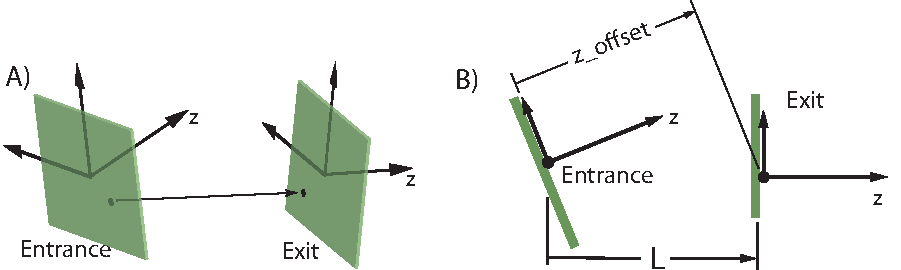
\includegraphics[width=5in]{patch.pdf}
  \caption[Patch Element.]
{A) A \vn{patch} element can align its exit face arbitrarily with respect to its entrance
face. B) The reference length of a \vn{patch} element is the longitudinal distance from
the entrance origin to the exit origin using the reference coordinates at the exit
end. Notice that while the length of the patch is defined with respect to the exit
coordinates, the offsets that define the position of the exit end coordinates are defined
with respect to the entrance coordinates.
}
  \label{f:patch}
\end{figure}

%-----------------

A \vn{patch} element shifts the reference orbit and time. Also see
\vn{floor_shift} (\sref{s:floor.ele}) and \vn{fiducial}
(\sref{s:fiducial}) elements.

General \vn{patch} element attributes are:
\begin{center}
\tt
\begin{tabular}{llll} \toprule
  {\sl Attribute Class}      & Section           & {\sl Attribute Class}      & Section         \\ \midrule
  Aperture limits            & \ref{s:limit}     & Offsets, pitches \& tilt   & \ref{s:offset}  \\ 
  Chamber wall               & \ref{s:wall}      & Reference energy           & \ref{s:energy}  \\
  Custom Attributes          & \ref{s:cust.att}  & Superposition              & \ref{s:super}   \\
  Description strings        & \ref{s:alias}     & Tracking \& transfer map   & \ref{c:methods} \\
  Length                     & \ref{s:l}         &                            &                 \\
  \bottomrule
\end{tabular}
\end{center}
\toffset
See \sref{s:list.patch} for a full list of element attributes.

\index{flexible}\index{e_tot_offset}
\index{x_offset}\index{y_offset}\index{z_offset}\index{tilt}
\index{x_pitch}\index{y_pitch}\index{t_offset}
\index{e_tot_set}\index{p0c_set}
Attributes specific to a \vn{patch} elements are:
\begin{example}
  x_offset        = <Real>    ! Exit face offset from Entrance.
  y_offset        = <Real>    ! Exit face offset from Entrance.
  z_offset        = <Real>    ! Exit face offset from Entrance.
  t_offset        = <Real>    ! Reference time offset.
  x_pitch         = <Real>    ! Exit face orientation from Entrance.
  y_pitch         = <Real>    ! Exit face orientation from Entrance.
  tilt            = <Real>    ! Exit face orientation from Entrance.
  e_tot_offset    = <Real>    ! Reference energy offset (eV).
  e_tot_set       = <Real>    ! Reference energy at exit end (eV).
  p0c_set         = <Real>    ! Reference momentum at exit end (eV).
  flexible        = <Logic>   ! Default: False.
  l               = <Real>    ! Reference length. Dependent attribute (\sref{s:depend}). 
\end{example}
\index{x_offset}

A straight line element like a \vn{drift} or a \vn{quadrupole} has the the exit face
parallel to the entrance face. With a \vn{patch} element, the entrance and exit faces can
be arbitrarily oriented with respect to one another as shown in \fig{f:patch}A. The length
\vn{l} of a \vn{patch} is a dependent (\sref{s:depend}) parameter and is the longitudinal
($z$ component) distance from the entrance origin to the exit origin using the exit end
reference coordinates as shown in \fig{f:patch}B. See \sref{s:patch.prob} for a further
discussion on the coordinate system of a \vn{patch}. Notice that while the length of the
patch is defined with respect to the exit coordinates, the offsets that define the
position of the exit end coordinates are defined with respect to the entrance coordinates.

\index{rigid patch}\index{infleible patch}
\index{flexible patch}
There are two different ways the orientation of the exit face is
determined. Which way is used is determined by the setting of the
\vn{flexible} attribute.  With the \vn{flexible} attribute set to
\vn{False}, the default, The exit face of the \vn{patch} will be
determined from the offset, tilt and pitch attributes as described in
\sref{s:patch.coords}. This type of \vn{patch} is called ``rigid'' or
``inflexible'' since the geometry of the \vn{patch} is solely
determined by the \vn{patch}'s attributes and is independent of
everything else.  Example:
\begin{example}
  pt: patch, z_offset = 3.2   ! Equivalent to a drift
\end{example}

With \vn{flexible} set to \vn{True}, the exit face is taken to be the
reference frame of the entrance face of the next element in the
lattice. In this case, it must be possible to compute the reference
coordinates of the next element before the reference coordinates of
the \vn{patch} are computed. A \vn{flexible} \vn{patch} will have the
its offsets, pitches, and tilt as dependent parameters
(\sref{s:depend}) and these parameters will be computed. Here the
\vn{patch} is called ``flexible'' since the geometry of the patch will
depend upon the geometry of the rest of the lattice and, therefore, if
the geometry of the rest of the lattice is modified (is ``flexed''),
the geometry of the \vn{patch} will vary as well. See
Section~\sref{s:ex.erl} for an example.

If a \vn{flexible} patch is within a \vn{multipass} (\sref{s:multipass})
region (as opposed to being just outside a multipass region as in
the example in Section~\sref{s:ex.erl}), the offsets, pitches, and tilt
will be computed using the geometry of the first pass.

With \vn{bmad_standard} tracking (\sref{s:tkm}) A particle, starting
at the upstream face of the \vn{patch}, is propagated in a straight
line to the downstream face and the suitable coordinate transformation
is made to translate the particle's coordinates from the upstream
coordinate frame to the downstream coordinate frame
(\sref{s:patch.std}). In this case the \vn{patch} element can be
thought of as a generalized \vn{drift} element.

If there are magnetic or electric fields within the \vn{patch}, the
tracking method through the \vn{patch} must be set to either
\vn{runge_kutta} or \vn{custom}. Example:
\begin{example}
  pa2: patch, tracking_method = runge_kutta, field_calc = custom, 
              mat6_calc_method = tracking, ...
\end{example}
In order to supply a custom field when \vn{runge_kutta} tracking is
used, \vn{field_calc} (\sref{s:integ}) needs to be set to
\vn{custom}. In this case, custom code must be supplied for
calculating the fields as a function of position
(\sref{s:custom.ele}).

The \vn{e_tot_offset} attribute offsets the
reference energy:
\begin{example}
  E_tot_ref(exit) = E_tot_ref(entrance) + E_tot_offset (eV)
\end{example}
Setting the \vn{e_tot_offset} attribute will affect a particle's
$p_x$, $p_y$ and $p_z$ coordinates via \Eqs{ppp} and \eq{ppppp}.
Notice that \vn{e_tot_offset} does not affect a particle's actual
energy, it just affects the difference between the particle energy and
the reference energy. 

Alternatively, to set the reference energy, the \vn{E_tot_set} or \vn{p0c_set} attributes
can be used to set the reference energy/momenum at the exit end. It is is an error
if more than one of \vn{e_tot_offset}, \vn{E_tot_set} and \vn{p0c_set} is nonzero.

\vn{Important}: \bmad may apply the energy transformation either before or after the
coordinate transformation. This matters when the speed of the reference particle is less
than $c$. For this reason, and due to complications involving PTC, it is recommended to
use two patches in a row when both the orbit and energy are to be patched.

The \vn{t_offset} attribute offsets the reference time so that the reference time at the exit end of
the patch \vn{t_ref(exit)} is related to the reference time at the beginning of the patch
\vn{t_ref(entrance)} via
\begin{example}
  t_ref(exit) = t_ref(entrance) + t_offset + dt_travel_ref
\end{example}
where \vn{dt_travel_ref} is the time for the reference particle to travel through the patch.
\vn{dt_travel_ref} is defined to be:
\begin{example}
  dt_travel_ref = L / beta_ref
\end{example}
Where \vn{L} is the length of the \vn{patch} as shown in \fig{f:patch}
and \vn{beta_ref} is the reference velocity/c at the exit end of the
element. That is, the reference energy offset is applied {\em before}
the reference particle is tracked through the patch. Since this point
can be confusing, it is recommended that a \vn{patch} element be split
into two consecutive patches if the \vn{patch} has finite \vn{l} and
\vn{E_tot_offset} values.

While a finite \vn{t_offset} will affect the reference time at the end of a patch, a finite
\vn{t_offset} will {\em not} affect the time that is calculated for a particle to reach the end of
the patch. On the other hand, a finite \vn{t_offset} will affect a particle's $z$ coordinate via
\Eqs{zbctt}. The change in $z$, $\delta z$ will be
\Begineq
  \delta z = \beta \cdot c \cdot \text{t_offset}
\Endeq
where $\beta$ is the normalized particle speed (which is independent of any energy patch). Another
way of looking at this is to note that In a drift, if the particle is on-axis and on-energy, t and
t_ref change but z does not change. In a time patch (a patch with only \vn{t_offset} finite), t_ref
and z change but t does not.

When a lattice branch contains both normally oriented and reversed elements
(\sref{s:ref.construct}), a \vn{patch}, or series of \vn{patches}, which reflects the $z$ direction
must be placed in between. See \sref{s:ex.patch} for an example. Such a \vn{patch}, (or patches) is
called a \vn{reflection} \vn{patch}. See Section~\sref{s:reflect.patch} for more details on how a
reflection patch is defined.

\index{wall}
Since the geometry of a \vn{patch} element is complicated, interpolation of the chamber wall in the
region of a patch follows special rules. See section~\sref{s:wall.vacuum} for more details.

%-----------------------------------------------------------------
\section{Photon_Init}
\label{s:photon.init}
\index{photon_init|hyperbf}

A \vn{photon_init} element is used as a starting element for x-ray
tracking.  A \vn{photon_init} element can be used to define such
things as the initial energy spectrum and angular orientation. As
explained below, a \vn{photon_init} element can be a ``stand alone''
photon source or it can have an associated ``physical source''
element.

General \vn{photon_init} attributes are:
\begin{center}
\tt
\begin{tabular}{llll} \toprule
  {\sl Attribute Class}      & Section           & {\sl Attribute Class}      & Section         \\ \midrule
  Aperture limits            & \ref{s:limit}     & Length                     & \ref{s:l}       \\
  Chamber wall               & \ref{s:wall}      & Offsets, pitches \& tilt   & \ref{s:offset}  \\
  Custom Attributes          & \ref{s:cust.att}  & Reference energy           & \ref{s:energy}  \\ 
  Description strings        & \ref{s:alias}     & Tracking \& transfer map   & \ref{c:methods} \\ 
  \bottomrule
\end{tabular}
\end{center}
\toffset
See \sref{s:list.photon.init} for a full list of element attributes.

\index{x_half_length}\index{y_half_length}
Attributes specific to an \vn{photon_init} element are:
\begin{example}
  ds_slice                 = <Real>
  E_center                 = <Real>    ! Average initial photon energy (eV).
  E_center_relative_to_ref = <Logic>   ! E_center relative to reference E?
  e_field_x                = <Real>    ! Polarization. x & y = 0 -> random
  e_field_y                = <Real>
  energy_distribution      = <Switch>  ! Gaussian or uniform
  physical_source          = <String>  ! physical source of x-rays
  ref_wavelength                       ! Reference wavelength (\sref{s:energy}). Dependent attribute (\sref{s:depend}).
  sig_x                    = <Real>
  sig_y                    = <Real>
  sig_z                    = <Real>
  sig_vx                   = <Real>
  sig_vy                   = <Real>
  sig_E                    = <Real>    ! Initial photon energy width (eV).
  spatial_distribution     = <Switch>  ! Gaussian or uniform. 
  transverse_sigma_cut     = <Real>
  velocity_distribution    = <Switch>  ! Gaussian, spherical, or uniform. 
\end{example}

  \begin{description}
  \index{ds_slice}
  \item[\vn{ds_slice}] \Newline
Used when there is an associated physical source element. The physical
source element is sliced into pieces of thickness \vn{ds_slice} and
each slice is tested to see if photons from the slice can possibly
pass through the first aperture. When photons are generated, photons
will only be generated from slices where they have a hope of passing
through the first aperture. This makes the simulation more efficient.
The default value of \vn{ds_slice} is 0.01 meter.

  \index{E_center}
  \item[\vn{E_center}] \Newline
Average initial photon energy in eV. If \vn{E_center_relative_to_ref}
is set to True, \vn{E_center} will be relative to the reference
energy.

  \index{E_center_relative_to_ref}
  \item[\vn{E_center_relative_to_ref}] \Newline
\vn{E_center} an absolute value (referenced to zero) if
\vn{E_center_relative_to_ref} is set to False. With a setting of True
(the default), \vn{E_center} is taken to be with respect to the
reference energy (\sref{s:ref.energy}). That is, if set to True, the
center energy \vn{<E>} is
\begin{example}
  <E> = E_center + Reference_Energy
\end{example}

  \index{e_field_x}\index{e_field_y}
  \item[\vn{e_field_x}, \vn{e_field_y}] \Newline
Electric field component of initial photons in the $x$ and $y$ planes.
If both are set to 0 then a random field is chosen with unit intensity
$E_x^2 + E_y^2 = 1$.

  \index{energy_distribution}
  \item[\vn{energy_distribution}] \Newline
Sets the type of energy spectrum for emitted photons. If there is an
associated physical element then this parameter is ignored and the
energy distribution is calculated from the physical element. Possible
settings are:
\begin{example2}
  gaussian   ! Default
  uniform
\end{example2}
The \vn{gaussian} setting gives a Gaussian distribution with width
set by \vn{sig_E}. The \vn{uniform} setting gives a flat
distribution in the range:
\begin{example2}
  [-sig_E, sig_E]
\end{example2}

  \index{physical_source}
  \item[\vn{physical_source}] \Newline
Used to specify the ``physical'' source of the photons. See below for more details

  \index{sig_E}
  \item[\vn{sig_E}] \Newline
Energy width in eV. See \vn{energy_distribution} for more
details.

  \index{sig_vx}\index{sig_vy}
  \item[\vn{sig_vx, sig_vy}] \Newline
Width of emitted photons in $v_x/c$ and $v_y/c$ directions. See
\vn{velocity_distribution} for more details.

  \index{sig_x}\index{sig_y}\index{sig_z}
  \item[\vn{sig_x, sig_y, sig_z}] \Newline
Width of emitted photons in $x$, $y$ and $z$ directions. See
\vn{spatial_distribution} for more details.

  \index{spatial_distribution}
  \item[\vn{spatial_distribution}] \Newline
Sets spacial $(x, y, z)$ spectrum of emitted photons. If there is an
associated physical element then this parameter is ignored and the
energy distribution is calculated from the physical element. Possible
settings are:
\begin{example2}
  gaussian    ! Default
  uniform
\end{example2}
The \vn{gaussian} setting gives a Gaussian distribution with width
set by \vn{sig_E}. The \vn{uniform} setting gives a flat
distribution in the range:
\begin{example2}
  [-sig_E, sig_E]
\end{example2}
The \vn{gaussian} setting gives a Gaussian distribution with width
$\sigma$ where $sigma$ is 
\begin{example2}
  sig_x     ! for x distribution
  sig_y     ! for y distribution
  sig_z     ! for z distribution
\end{example2}
The \vn{uniform} setting gives a flat
distribution in the range: $[-\sigma, \sigma]$.

  \index{velocity_distribution}
  \item[\vn{velocity_distribution}] \Newline
Sets the transverse $(v_x/c, v_y/c)$ velocity spectrum of emitted
photons. If there is an associated physical element then this
parameter is ignored and the energy distribution is calculated from
the physical element. The longitudinal velocity is always computed to
make $v_x^2 + v_y^2 + v_z^2 = c^2$ Possible settings are:
\begin{example2}
  gaussian    ! Default
  spherical
  uniform
\end{example2}
The \vn{gaussian} setting gives a Gaussian distribution with width
$\sigma$ where $sigma$ is 
\begin{example2}
  sig_vx     for vx/c distribution
  sig_vy     for vy/c distribution
\end{example2}
The \vn{uniform} setting gives a flat distribution in the range:
$[-\sigma, \sigma]$.
The \vn{spherical} setting gives flat distribution in all directions.
  \end{description}

For the purposes of positioning the elements in the lattice around it,
a \vn{photon_init} element is considered to have zero length.

\vn{photon_init} elements are used in one of two modes: With or
without an associated physical source element specified by the
\vn{physical_source} attribute. Without an associated physical source,
the \vn{photon_init} element completely specifies the initial photon
distribution. With an associated physical source element, the photon
distribution is determined by the physical source but the shape of the
energy spectrum can be modified by setting attributes in the
\vn{photon_init} element. Example:
\begin{example}
  b05w: sbend, l = 3.2, angle = 0.1
  pfork: photon_fork, to_line = c_line, superimpose, ref = b05w, offset = 0.4
  bend_line: line = (..., b05w, ...)
  use bend_line

  c_line: line = (pinit, ...)
  c_line[e_tot] = 15e3
  pinit: photon_init, physical_source = 'b05w', sig_E = 2.1
\end{example}
In this example, the bend \vn{b05w} is a bend producing photons. It is
part of the line \vn{bend_line}. \vn{bend_line} also contains a
\vn{photon_fork} element named \vn{pfork} which branches to the line
\vn{c_line}. \vn{c_line} contains the \vn{photon_init} element
\vn{pinit} which references \vn{b03w} as the associated physical
source element. When photons are tracked, they are generated in
\vn{b05w} and then propagated to the \vn{pfork} fork.  After this they
are propagated through \vn{c_line}. The \vn{pinit} element acts like a
zero length \vn{marker} element when photons propagate through
it. That is, the \vn{pinit} element essentially serves to associate
\vn{c_line} with \vn{b03w} for the purposes of photon tracking. Also,
in this example, \vn{pinit} modifies the photon energy spectrum so
that only photons whose energy is within 2.1 eV are generated

It is important to note that in the above example, with the
\vn{photon_init} element having an associated physical source, the
setting of things like the spatial shape \vn{sig_z}, etc. in the
\vn{photon_init} element will be ignored.

%-----------------------------------------------------------------
\section{Quadrupole}
\label{s:quad}
\index{quadrupole|hyperbf}

A \vn{quadrupole} is a magnetic element with a linear field dependence
with transverse offset (\sref{s:mag.field}).

General \vn{quadrupole} attributes are:
\begin{center}
\tt
\begin{tabular}{llll} \toprule
  {\sl Attribute Class}      & Section           & {\sl Attribute Class}      & Section            \\ \midrule
  Aperture limits            & \ref{s:limit}     & Mag \& Elec multipoles     & \ref{s:multip}     \\
  Chamber wall               & \ref{s:wall}      & Offsets, pitches \& tilt   & \ref{s:offset}     \\
  Description strings        & \ref{s:alias}     & Overlapping Fields         & \ref{s:overlap}    \\
  Fringe Fields              & \ref{s:fringe}    & Reference energy           & \ref{s:energy}     \\ 
  Hkick \& Vkick             & \ref{s:kick}      & Superposition              & \ref{s:super}      \\
  Integration settings       & \ref{s:integ}     & Symplectify                & \ref{s:symp}       \\
  Is_on                      & \ref{s:is.on}     & Field Maps                 & \ref{s:fieldmap}   \\ 
  Length                     & \ref{s:l}         & Tracking \& transfer map   & \ref{c:methods}    \\ 
  \bottomrule
\end{tabular}
\end{center}
\toffset
See \sref{s:list.quadrupole} for a full list of element attributes.

\index{f1}\index{f2}
\index{k1}\index{b1_gradient}
Attributes specific to a \vn{quadrupole} element are:
\begin{example}
  b1_gradient    = <Real>    ! Field strength. (\sref{s:depend}).
  k1             = <Real>    ! Quadrupole strength.
  fq1            = <Real>    ! Soft edge fringe parameter.
  fq2            = <Real>    ! Soft edge fringe parameter.
 \end{example}

\index{tilt}
If the \vn{tilt} attribute is present without a value then a value of $\pi/4$
is used.

For a quadrupole with zero \vn{tilt} and a positive \vn{k1}, the
quadrupole is horizontally focusing and vertically defocusing
(\sref{s:mag.field}).

The \vn{fq1} and \vn{fq2} parameters are used to specify the
quadrupolar ``soft'' edge fringe. See \sref{s:q.soft} for more details.
The \vn{fringe_at} and \vn{fringe_type} settings (\sref{s:fringe})
determine if the fringe field is used in tracking (\sref{s:fringe}).

Example:
\begin{example}
  q03w: quad, l = 0.6, k1 = 0.003, tilt  ! same as tilt = pi/4
\end{example}

%-----------------------------------------------------------------
\section{RFcavity}
\label{s:rfcav}
\index{rfcavity|hyperbf}

An \vn{rfcavity} is an RF cavity without acceleration generally used
in a storage ring. The main difference between an \vn{rfcavity} and an
\vn{lcavity} is that, unlike an \vn{lcavity}, the reference energy
(\sref{s:phase.space}) through an \vn{rfcavity} is constant.

General \vn{rfcavity} attributes are:
\begin{center}
\tt
\begin{tabular}{llll} \toprule
  {\sl Attribute Class}      & Section            & {\sl Attribute Class}      & Section            \\ \midrule
  Aperture limits            & \ref{s:limit}      & Offsets, pitches \& tilt   & \ref{s:offset}     \\
  Chamber wall               & \ref{s:wall}       & Overlapping Fields         & \ref{s:overlap}    \\
  Custom Attributes          & \ref{s:cust.att}   & Reference energy           & \ref{s:energy}     \\ 
  Description strings        & \ref{s:alias}      & RF Couplers                & \ref{s:rf.coupler} \\
  Field autoscaling          & \ref{s:autoscale}  & Superposition              & \ref{s:super}      \\
  Fringe Fields              & \ref{s:fringe}     & Symplectify                & \ref{s:symp}       \\
  Hkick \& Vkick             & \ref{s:kick}       & Field Maps                 & \ref{s:fieldmap}   \\
  Integration settings       & \ref{s:integ}      & Tracking \& transfer map   & \ref{c:methods}    \\
  Is_on                      & \ref{s:is.on}      & Wakes                      & \ref{s:wakes}      \\
  Length                     & \ref{s:l}          &                            &                    \\
  \bottomrule
\end{tabular}
\end{center}
\toffset
See \sref{s:list.rfcavity} for a full list of element attributes.

\index{rf_frequency}\index{harmon}\index{voltage}\index{phi0}\index{phi0_multipass}\index{harmon_master}
Attributes specific to an \vn{rfcavity} are:
\begin{example}
  rf_frequency    = <Real>    ! Frequency
  harmon          = <Real>    ! Harmonic number
  voltage         = <Real>    ! Cavity voltage
  phi0            = <Real>    ! Cavity phase
  phi0_multipass  = <Real>    ! Phase variation with multipass
  gradient        = <Real>    ! Accelerating gradient (V/m). Dependent attribute (\sref{s:depend}).
\end{example}

The \vn{phi0} attribute here is identical to the \vn{lag} attribute of
\mad. The integrated energy kick felt by a particle, assuming no phase slippage, is 
\begin{example}
  dE = -e_charge * voltage * sin(\(2\,\pi\) * (\(\phi_\text{t}\) - \(\phi_\text{ref}\)))
\end{example}
\index{multipass}
where
\begin{example}
  \(\phi_\text{ref}\) = phi0 + phi0_multipass + phi0_autoscale
\end{example}
and $\phi_t$ is the part of the phase due to when the particle arrives
at the cavity and depends upon whether \vn{absolute time tracking} or 
\vn{relative time tracking} as discussed in \sref{s:rf.time}.

\vn{phi0_multipass} is only to be used to shift the phase with respect
to a \vn{multipass} lord. See \sref{s:multipass}. \vn{e_charge} is the
charge on an electron (Table~\ref{t:constants}). Notice that the
energy kick is independent of the sign of the charge of the particle

\vn{phi0_autoscale} and \vn{field_autoscale} are calculated by \bmad's auto-scale
module. See Section~\sref{s:autoscale} for more details. Autoscaling can be toggled on/off
by using the \vn{autoscale_phase} and \vn{autoscale_amplitude} toggles.

If \vn{harmon} is non--zero the \vn{rf_frequency} is calculated by
\begin{example}
  rf_frequency = harmon * c_light * beta0 / L_lattice 
\end{example}
where \vn{L_lattice} is the total lattice length and \vn{beta0} is the
velocity of the reference particle at the start of the lattice. After
the lattice has been read in, \vn{rf_frequency} will be the
independent variable (\sref{s:depend}).

Couplers (\sref{s:rf.coupler}) and HOM wakes (\sref{s:wakes}) can
be modeled. In addition, if a field map is specified
(\sref{s:fieldmap}), tracking using an integrator is possible.

\index{RF field map}
\index{runge_kutta!and field maps}\index{adaptive_runge_kutta!and field maps}
\index{boris!and field maps}\index{symp_lie_bmad!and field maps}
If a field map is specified (\sref{s:fieldmap}), tracking using an
integrator is possible. A field map is only used for \vn{runge_kutta},
\vn{adaptive_runge_kutta}, \vn{boris} and \vn{symp_lie_bmad} tracking
(\sref{s:tkm}).  Only the fundamental mode has an analytical formula
for the symplectic tracking. In the future, the other modes could be
used with \vn{symp_lie_bmad} tracking using a field expansion about
the centerline.

The \vn{cavity_type} is the type of cavity being simulated. Possible
settings are:
\begin{example}
  ptc_standard
  standing_wave    ! Default
  traveling_wave
\end{example}
The \vn{cavity_type} switch is ignored if a field map is used.

Example:
\begin{example}
  rf1: rfcav, l = 4.5, harmon = 1281, voltage = 5e6
\end{example}

%-----------------------------------------------------------------
\section{Sad_Mult}
\label{s:sad.mult}
\index{sad_mult|hyperbf}

A \vn{sad_mult} element is equivalent to a SAD\cite{b:sad} \vn{mult}
element. This element is a combination solenoid, multipole, bend, and
RF cavity.

General \vn{sample} attributes are:
\begin{center}
\tt
\begin{tabular}{llll} \toprule
  {\sl Attribute Class}      & Section           & {\sl Attribute Class}      & Section         \\ \midrule
  a$n$, b$n$ multipoles      & \ref{s:multip}    & Length                     & \ref{s:l}       \\
  Aperture limits            & \ref{s:limit}     & Offsets, pitches \& tilt   & \ref{s:offset}  \\
  Chamber wall               & \ref{s:wall}      & Reference energy           & \ref{s:energy}  \\ 
  Custom Attributes          & \ref{s:cust.att}  & Superposition              & \ref{s:super}   \\
  Description strings        & \ref{s:alias}     & Tracking \& transfer map   & \ref{c:methods} \\ 
  Fringe Fields              & \ref{s:fringe}    &                            &                 \\
  \bottomrule
\end{tabular}
\end{center}
\toffset
See \sref{s:list.sad.mult} for a full list of element attributes.

\index{angle}\index{bs_field}\index{e1}\index{e2}\index{eps_step_scale}
\index{f1}\index{f2}\index{g}\index{rf_frequency}\index{harmon}
\index{ks}\index{phi0}\index{rho}\index{voltage}\index{x_offset_mult}
\index{y_offset_mult}\index{x_pitch_mult}\index{y_pitch_mult}
\index{fringe_type}\index{kill_fringe}
Attributes specific to an \vn{sextupole} element are:
\begin{example}
  bs_field        = <Real>    ! Solenoid field. SAD equivalent: BZ.
  e1, e2          = <Real>    ! Bend face angles.
  eps_step_scale  = <Real>    ! Step size scale. Default = 1. SAD equivalent: EPS.
  fq1             = <Real>    ! Quadrupole fringe integral. SAD equivalent: F1.
  fq2             = <Real>    ! Quadrupole fringe integral. SAD equivalent: F2.
  ks              = <Real>    ! Solenoid strength. 
  x_offset_mult   = <Real>    ! Mult component offset. SAD equivalent: DX.
  y_offset_mult   = <Real>    ! Mult component offset. SAD equivalent: DY.
  x_pitch_mult    = <Real>    ! Mult component pitch. SAD equivalent: DPX or CHI1.
  y_pitch_mult    = <Real>    ! Mult component pitch. SAD equivalent: DPY or CHI2.
  fringe_type     = <Switch>  ! Type of fringe. SAD equivalent: DISFRIN.
  fringe_at       = <Switch>  ! Where fringe is applied. SAD equivalent: FRINGE.
\end{example}

%  angle           = <Real>    ! Bend angle. A settable dependent variable (\sref{s:depend})
%  g               = <Real>    ! Bend strength 1/rho
%  rf_frequency    = <Real>    ! Rf frequency (Hz). SAD equivalent: FREQ.
%  harmon          = <Real>    ! Harmonic number. SAD equivalent: HARM.
%  phi0            = <Real>    ! Cavity phase. SAD equivalent: PHI.
%  rho             = <Real>    ! Bend radius. A settable dependent variable (\sref{s:depend})
%  voltage         = <Real>    ! Cavity voltage. SAD equivalent: VOLT.

One difference between SAD and \bmad is that SAD defines the solenoid
field by what are essentially a set of marker elements so that the
solenoid field at a SAD \vn{mult} element is not explicitly declared
in the \vn{mult} element definition. \bmad, on the other hand,
requires a \vn{sad_mult} element to explicitly declare the solenoid
parameters.

Another difference between SAD and \bmad is that, within a solenoid,
the reference trajectory is aligned with the solenoid axis (and not
aligned with the axis of the elements within the solenoid region).

The SAD \vn{mult} element uses normal \vn{Kn} and skew \vn{KSn}
multipole components. The \bmad \vn{sad_mult} element used normal
\vn{an} and skew \vn{bn} multipole components. As can be seen from the
equations in \sref{s:mag.field}, there is a factor of $n!$ between the
two representations.

The \vn{fq1} and \vn{fq2} parameters are used to specify the
quadrupolar ``soft'' edge fringe. See \sref{s:q.soft} for more details.

The \vn{fringe_at} and \vn{fringe_type} settings determine if the fringe field is used in
tracking. See Sec~\sref{s:fringe} for the translation between these two switches and the
\vn{fringe} and \vn{disfrin} switches of SAD.

Unlike other elements, the \vn{ds_step} and \vn{num_steps} attributes (\sref{s:integ}) of a \vn{sad_mult}
are dependent attributes (\sref{s:depend}) and are not directly settable. Rather these
attributes are calculated using \vn{SAD}'s own algorithm for setting the step size. To
vary the calculated step size for a single \vn{sad_mult} element, the attribute
\vn{eps_step_scale} may be set.  To vary the step size for all \vn{sad_mult} elements, the
global parameter \vn{bmad_com[sad_eps_scale]} (\sref{s:bmad.com}) may be set.
The default values for these parameters are:
\begin{example}
  eps_step_scale          = 1
  bmad_com[sad_eps_scale] = 5e-3
\end{example}

SAD conventions to be aware of when comparing SAD to Bmad:
\begin{itemize}
\item
A SAD \vn{rotate} or \vn{chi3} rotation is opposite to a \bmad \vn{tilt}
\item
SAD element offsets (\vn{dx}, \vn{dy}, \vn{dz}) are with respect to the entrance end
of the element as opposed to \bmad's convention of referencing to the element center.
\item
  The \bmad \vn{sad_mult} element does not have any attributes corresponding to the following
SAD \vn{MULT} element attributes:
\begin{example}
  angle, harmon, freq, phi, dphi, volt, dvolt
\end{example}
\end{itemize}

%-----------------------------------------------------------------
\section{Sample}
\label{s:sample}
\index{sample|hyperbf}

A \vn{sample} element is used to simulate a material sample which is illuminated by x-rays.

General \vn{sample} attributes are:
\begin{center}
\tt
\begin{tabular}{llll} \toprule
  {\sl Attribute Class}      & Section           & {\sl Attribute Class}      & Section         \\
  Aperture limits            & \ref{s:limit}     & Offsets, pitches \& tilt   & \ref{s:offset}  \\ \midrule
  Chamber wall               & \ref{s:wall}      & Reference energy           & \ref{s:energy}  \\ 
  Custom Attributes          & \ref{s:cust.att}  & Surface Properties         & \ref{s:s.curve} \\
  Description strings        & \ref{s:alias}     & Superposition              & \ref{s:super}   \\
  Integration settings       & \ref{s:integ}     & Tracking \& transfer map   & \ref{c:methods} \\
  Length                     & \ref{s:l}         &                            &                 \\
  \bottomrule
\end{tabular}
\end{center}
\toffset
See \sref{s:list.sample} for a full list of element attributes.

This element is in development.

Attributes specific to an \vn{solenoid} element are:
\begin{example}
  mode       = <Switch> ! Reflection or transmission.
  material   = <type>   ! Type of material. \sref{s:cryst.list}
\end{example}

The \vn{mode} parameter can be set to:
\begin{example}
  reflection
  transmission
\end{example}
With \vn{mode} set to \vn{reflection}, photons will be back scattered
from the sample surface isotropically. In this case the material
properties will not matter. Additionally, a \vn{patch}
(\sref{s:patch}) element will be needed after the \vn{sample} element
to properly reorient the reference orbit.

With \vn{mode} set to \vn{transmission}, photons will be transmitted
through the sample. In this case \vn{material} will be used to
determine the attenuation and phase shift of the photons.

Example:
\begin{example}
  formula409: sample, x_limit = 10e-3, y_limit = 20e-3, mode = reflection
\end{example}

%-----------------------------------------------------------------
\section{Sextupole}
\label{s:sex}
\index{sextupole|hyperbf}

A \vn{sextupole} is a magnetic element with a quadratic field
dependence with transverse offset (\sref{s:mag.field}).

General \vn{sextupole} attributes are:
\begin{center}
\tt
\begin{tabular}{llll} \toprule
  {\sl Attribute Class}      & Section           & {\sl Attribute Class}      & Section           \\ \midrule
  Aperture limits            & \ref{s:limit}     & Mag \& Elec multipoles     & \ref{s:multip}    \\
  Chamber wall               & \ref{s:wall}      & Offsets, pitches \& tilt   & \ref{s:offset}    \\
  Custom Attributes          & \ref{s:cust.att}  & Overlapping Fields         & \ref{s:overlap}   \\
  Description strings        & \ref{s:alias}     & Reference energy           & \ref{s:energy}    \\ 
  Fringe Fields              & \ref{s:fringe}    & Superposition              & \ref{s:super}     \\
  Hkick \& Vkick             & \ref{s:kick}      & Symplectify                & \ref{s:symp}      \\
  Integration settings       & \ref{s:integ}     & Field Maps                 & \ref{s:fieldmap}  \\
  Is_on                      & \ref{s:is.on}     & Tracking \& transfer map   & \ref{c:methods}   \\ 
  Length                     & \ref{s:l}         &                            &                   \\ 
  \bottomrule
\end{tabular}
\end{center}
\toffset
See \sref{s:list.sextupole} for a full list of element attributes.

\index{k2}
\index{b2_gradient}
Attributes specific to an \vn{sextupole} element are:
\begin{example}
  k2          = <Real>   ! Sextupole strength.
  b2_gradient = <Real>   ! Field strength. (\sref{s:depend}).
\end{example}

The \vn{bmad_standard}
calculation treats a sextupole using a kick--drift--kick model.

If the \vn{tilt} attribute is present without a value then a value of 
$\pi/6$ is used.
Example:
\begin{example}
  q03w: sext, l = 0.6, k2 = 0.3, tilt  ! same as tilt = pi/6
\end{example}

%-----------------------------------------------------------------
\section{Solenoid}
\label{s:sol}
\index{solenoid|hyperbf}

A \vn{solenoid} is an element with a longitudinal magnetic field.

General \vn{solenoid} attributes are:
\begin{center}
\tt
\begin{tabular}{llll} \toprule
  {\sl Attribute Class}      & Section           & {\sl Attribute Class}      & Section            \\ \midrule
  Aperture limits            & \ref{s:limit}     & Mag \& Elec multipoles     & \ref{s:multip}     \\
  Chamber wall               & \ref{s:wall}      & Offsets, pitches \& tilt   & \ref{s:offset}     \\
  Custom Attributes          & \ref{s:cust.att}  & Overlapping Fields         & \ref{s:overlap}    \\
  Description strings        & \ref{s:alias}     & Reference energy           & \ref{s:energy}     \\ 
  Fringe Fields              & \ref{s:fringe}    & Superposition              & \ref{s:super}      \\
  Hkick \& Vkick             & \ref{s:kick}      & Symplectify                & \ref{s:symp}       \\
  Integration settings       & \ref{s:integ}     & Field Maps                 & \ref{s:fieldmap}   \\
  Is_on                      & \ref{s:is.on}     & Tracking \& transfer map   & \ref{c:methods}    \\ 
  Length                     & \ref{s:l}         &                            &                    \\ 
  \bottomrule
\end{tabular}
\end{center}
\toffset
See \sref{s:list.solenoid} for a full list of element attributes.

\index{ks}
\index{bs_gradient}
Attributes specific to an \vn{solenoid} element are:
\begin{example}
  ks         = <Real>   ! Solenoid strength.
  bs_field   = <Real>   ! Field strength. (\sref{s:depend}).
\end{example}

The \vn{bmad_standard} tracking model (\sref{s:tkm}) uses a ``hard
edge'' model where an impulse kick is applied at the entrance and exit
ends of the element due to the fringe fields there.

Example:
\begin{example}
  cleo_sol: solenoid, l = 2.6, ks = 1.5e-9 * parameter[e_tot]
\end{example}

%-----------------------------------------------------------------
\section{Sol_Quad}
\label{s:sq}
\index{sol_quad|hyperbf}

A \vn{sol_quad} is a combination solenoid/quadrupole.

General \vn{sol_quad} attributes are:
\begin{center}
\tt
\begin{tabular}{llll} \toprule
  {\sl Attribute Class}      & Section           & {\sl Attribute Class}      & Section            \\ \midrule
  Aperture limits            & \ref{s:limit}     & Mag \& Elec multipoles     & \ref{s:multip}     \\
  Chamber wall               & \ref{s:wall}      & Offsets, pitches \& tilt   & \ref{s:offset}     \\
  Custom Attributes          & \ref{s:cust.att}  & Overlapping Fields         & \ref{s:overlap}    \\
  Description strings        & \ref{s:alias}     & Reference energy           & \ref{s:energy}     \\ 
  Fringe Fields              & \ref{s:fringe}    & Superposition              & \ref{s:super}      \\
  Hkick \& Vkick             & \ref{s:kick}      & Symplectify                & \ref{s:symp}       \\
  Integration settings       & \ref{s:integ}     & Field Maps                 & \ref{s:fieldmap}   \\
  Is_on                      & \ref{s:is.on}     & Tracking \& transfer map   & \ref{c:methods}    \\ 
  Length                     & \ref{s:l}         &                            &                    \\ 
  \bottomrule
\end{tabular}
\end{center}
\toffset
See \sref{s:list.sol.quad} for a full list of element attributes.

\index{k1}\index{ks}\index{bs_field}\index{b1_gradient}
Attributes specific to a \vn{sol_quad} element are:
\begin{example}
  k1          = <Real>    ! Quadrupole strength.
  ks          = <Real>    ! Solenoid strength.
  bs_field    = <Real>    ! Solenoid Field strength.
  b1_gradient = <Real>    ! Quadrupole Field strength.
\end{example}

Example:
\begin{example}
  sq02: sol_quad, l = 2.6, k1 = 0.632, ks = 1.5*beam[energy]
\end{example}

%-----------------------------------------------------------------
\section{Taylor}
\label{s:taylor}
\index{taylor|hyperbf}

A \vn{taylor} is a Taylor map (\sref{s:taylor.phys}). This can be used
in place of the \mad \vn{matrix} element.

General \vn{taylor} attributes are:
\begin{center} 
\tt
\begin{tabular}{llll} \toprule
  {\sl Attribute Class}      & Section          & {\sl Attribute Class}      & Section         \\ \midrule
  Aperture limits            & \ref{s:limit}    & Offsets \& tilt            & \ref{s:offset}  \\
  Custom Attributes          & \ref{s:cust.att} & Reference energy           & \ref{s:energy}  \\
  Description strings        & \ref{s:alias}    & Superposition              & \ref{s:super}   \\
  Is_on                      & \ref{s:is.on}    & Symplectify                & \ref{s:symp}    \\
  Length                     & \ref{s:l}        & Tracking \& transfer map   & \ref{c:methods} \\

  \bottomrule
\end{tabular}
\end{center}
\toffset
See \sref{s:list.taylor} for a full list of element attributes.

Attributes specific to a \vn{taylor} element are:
\begin{example}
  ref_orbit = (<x>, <px>, <y>, <py>, <z>, <pz>)     ! Reference orbit.
  x_ref = <Real>                                    ! $x$ reference orbit component.
  px_ref = <Real>                                   ! $p_x$ reference orbit component.
  y_ref = <Real>                                    ! $y$ reference orbit component.
  py_ref = <Real>                                   ! $p_y$ reference orbit component.
  z_ref = <Real>                                    ! $z$ reference orbit component.
  pz_ref = <Real>                                   ! $p_z$ reference orbit component.
  \{<out>: <coef>, <e1> <e2> <e3> <e4> <e5> <e6>\}    ! Taylor term. First form.
  \{<out>: <coef> | <n1> <n2> ...\}                   ! Taylor term. Second form.
  tt<out><n1><n2>...  = <Coef>                      ! Taylor term. Third form.
\end{example}

For historical reasons, there are three differnt forms that can be used to specify a
taylor term.  Notice that the first form (above) uses a comma ``,'' to separate the
\vn{<coef>} from \vn{<e1>}, while the second form uses a vertical bar ``|'' to separate
\vn{<coef>} from \vn{<n1>}.

A Taylor term has a coefficient \vn{<coef>} which is a real number,
integer exponents \vn{<e1>}, \vn{<n1>}, etc., and \vn{<out>} signifies
which output variable the Taylor term is associated with.  For orbital
phase space variables \vn{<Out>} is an integer in the range 1 to 6
with \vn{<out>} = 1 for $x$, etc. For terms associated with spin,
\vn{<out>} is a two character string with each character being
one of ``\vn{x}'', ``\vn{y}'', or ``\vn{z}''. 

For orbital phase space variables a term in a Taylor map is of the form
\Begineq
  r_j(\Out) = C \cdot \Pi_{i = 1}^6 \, \delta r_i^{e_i}
\Endeq
where $\bfr = (x, p_x, y, p_y, z, p_z)$ and $\delta \bfr = \bfr(\In) - \bfr_\Ref$ with
$\bfr_\Ref$ begin the reference orbit. A term in a Taylor map can be specified by one of
two forms as shown above. The first form specifies the six exponents $e_i$ using the
integers \vn{<e1>} corresponding to $e_1$, \vn{<e2>} corresponding to $e_2$, etc.  For
example, a term in a Taylor map that was
\Begineq
  p_y(\Out) = 2.73 \cdot \delta y^2(\In) \, \delta p_z(\In)
\Endeq
would be written as
\begin{example}
  \{4: 2.73, 0 0 2 0 0 1\}
\end{example}

The second form for specifying a Taylor term uses a set of integers \vn{<n1>},
\vn{<n2>}, etc. Each integer must be between 1 and 6 inclusive. The value of 
the $i$\Th exponent $e_i$ is equal to the number of integers that are equal
to $i$. For example, the term of the above example would be written using
the second form as
\begin{example}
  \{4: 2.73 | 336\}
\end{example}
Notice that with the second form, spaces between exponent terms is optional.

The third form is like the second form. For example, the term of the above examples
would be written unsing the third form as:
\begin{example}
  tt4336 = 2.73
\end{example}

For spin, a Taylor map is associated with one of the components in the
3x3 spin map matrix (\sref{s:spin.map}). An individual Taylor term is
of the form
\Begineq
  S_j(\Out) = C \cdot \Pi_{i = 1}^6 \, \delta r_i^{e_i}(\In) \, S_k(\In)
\Endeq
For example
\begin{example}
  \{xz: 0.43 | 13 \}
\end{example}
is equivalent to
\Begineq
  S_x(\Out) = 0.43 \cdot \delta x(\In) \, \delta y(\In) \, S_z(\In)
\Endeq

By default, a \vn{taylor} element starts out with the unit phase space map but no default
is defined for the spin part of the map.  That is, a \vn{taylor} element starts with the
following 6 terms
\begin{example}
  \{1: 1.0, 1 0 0 0 0 0\}
  \{2: 1.0, 0 1 0 0 0 0\}
  \{3: 1.0, 0 0 1 0 0 0\}
  \{4: 1.0, 0 0 0 1 0 0\}
  \{5: 1.0, 0 0 0 0 1 0\}
  \{6: 1.0, 0 0 0 0 0 1\}
\end{example}
Which is equivalent to
\begin{example}
  \{1: 1.0 | 1\}
  \{2: 1.0 | 2\}
  \{3: 1.0 | 3\}
  \{4: 1.0 | 4\}
  \{5: 1.0 | 5\}
  \{6: 1.0 | 6\}
\end{example}

The \vn{ref_orbit} attribute specifies the phase space $(x, px, y, py, z, pz)$ reference
orbit at the start of the element used to construct the Taylor map. Alternatively, the
individual components of the reference orbit may be specified by using the attributes 
\vn{x_ref}, \vn{px_ref}, \vn{y_ref}, \vn{py_ref}, \vn{z_ref}, or \vn{pz_ref}.

Note: when converting the map from \bmad to PTC (\sref{c:ptc}), the \bmad/PTC interface
code will convert from Bmad phase space coordinates to PTC phase space coordinates and
will convert the map to using the reference orbit as the map zero orbit. This does not
affect tracking but will affect map analysis.

A term in a \vn{taylor} element will override any previous term
with the same \vn{out} and \vn{e1} through \vn{e6} indexes. For example the term:
\begin{example}
  tt: Taylor, \{1: 4.5, 1 0 0 0 0 0\} 
\end{example}
will override the default \vn{\{1: 1.0, 1 0 0 0 0 0\}} term.

The \vn{l} length attribute of a \vn{taylor} element does not affect phase space
coordinates but will affect the longitudinal $s$ position of succeeding elements and will
affect the time it takes a particle to track through the element.

A \vn{taylor} element that is ``turned off'' (\vn{is_on} attribute set to False), is
considered to be like a \vn{marker} element. That is, the orbit and twiss parameters are
unchanged when tracking through a \vn{taylor} element that is turned off.

Example \vn{taylor} element definition:
\begin{example}
  tt: Taylor, \{4:  2.7, 0 0 2 0 0 1\}, \{2:  1.9 | 1 1 2\},
              \{xz: 0.43 | 2 \}, ..., 
              ref_orbit = (0.01, 0.003, 0.002, 0.001, 0.0, 0.2)
\end{example}

Note: Tracking through a \vn{taylor} elements using \vn{symp_lie_ptc} is the same as
tracking with the \vn{taylor} tracking method.  That is, the Taylor map is simply
evaluated and no effort at symplectification is done. Furthermore, evaluating the Taylor
map of a \vn{taylor} element using the \vn{taylor} method is faster than evaluation using
\vn{symp_lie_ptc}. Thus the \vn{taylor} tracking method should always be used with
\vn{taylor} elements.


%-----------------------------------------------------------------
\section{Wiggler and Undulator} 
\label{s:wiggler}
\index{wiggler|hyperbf} 
\index{undulator|hyperbf} 

A \vn{wiggler} or \vn{undulator} element is basically a periodic array of alternating bends.
The only difference between \vn{wigglers} and \vn{undulators} is in the x-ray emission spectrum.
Charged particle tracking will be the same. 

Henceforth, the term ``wiggler'' will denote either a \vn{wiggler} or \vn{undulator}

General \vn{wiggler} attributes are:
\begin{center}
\tt
\begin{tabular}{llll} \toprule
  {\sl Attribute Class}      & Section           & {\sl Attribute Class}      & Section            \\ \midrule
  Aperture limits            & \ref{s:limit}     & Mag \& Elec multipoles     & \ref{s:multip}     \\
  Chamber wall               & \ref{s:wall}      & Offsets, pitches \& tilt   & \ref{s:offset}     \\
  Custom Attributes          & \ref{s:cust.att}  & Overlapping Fields         & \ref{s:overlap}    \\
  Description strings        & \ref{s:alias}     & Reference energy           & \ref{s:energy}     \\ 
  Fringe Fields              & \ref{s:fringe}    & Superposition              & \ref{s:super}      \\
  Hkick \& Vkick             & \ref{s:kick}      & Symplectify                & \ref{s:symp}       \\
  Integration settings       & \ref{s:integ}     & Field Maps                 & \ref{s:fieldmap}   \\
  Is_on                      & \ref{s:is.on}     & Tracking \& transfer map   & \ref{c:methods}    \\ 
  Length                     & \ref{s:l}         &                            &                    \\ 
  \bottomrule
\end{tabular}
\end{center}
\toffset
See \sref{s:list.wiggler} for a full list of element attributes.

There are two types of wigglers. Those that that are described using a
magnetic field map (``map type'') and those that are described
assuming a periodic field (``periodic type''). 

%-----------------------------------------------------
\subsection{Map\_Type Wigglers}
\label{s:wiggler.map}

The \vn{map type} wigglers are modeled using the Cartesian mode
decomposition of Sec.~\sref{s:cart.map}. 

\index{polarity}
\index{term (for a wiggler)}
Attributes specific to a \vn{map type} \vn{wiggler} element are:
\begin{example}
  b_max    = <Real>   ! Maximum magnetic field (in T) on the wiggler centerline. 
                      !   Dependent attribute (\sref{s:depend}).
  polarity = <Real>   ! For scaling the field.
\end{example}

The \vn{polarity} value is used to scale the magnetic field. By
default, \vn{polarity} has a value of 1.0.  Example:
\begin{example}
  wig1: wiggler, l = 1.6, polarity = -1, cartesian_map = \{...\}
\end{example}

The \vn{b_max} attribute for a \vn{map type} \vn{wiggler} is the
maximum field computed for \vn{polarity} = 1.

There is no \vn{bmad_standard} tracking for a \vn{map_type}
\vn{wiggler}. \vn{symp_lie_bmad} type tracking is discussed in \sref{s:symp.track}

%-----------------------------------------------------
\subsection{Old Map\_Type Wigglers Syntax}
\label{s:old.wiggler}

When the wiggler model was first developed, the definition of the field was somewhat
different and there was a special syntax for specifying the field. The old syntax looked
like
\Begineq
  \text{term(i)} = \{C, k_x, k_y, k_z, \phi_z \}
\Endeq
Example:
\begin{example}
  wig1: wiggler, l = 1.6, 
        term(1) = \{0.03, 3.00, 4.00, 5.00, 0.63\},
        term(2) = ...
\end{example}

The old definition used only the three forms corresponding to the \vn{cartesian_map}
\vn{y} family (\sref{s:cart.map.phys}) with $x_0 = y_0 = 0$. There was also a different
normalization convention. The old style \vn{hyper-y} form was
\begin{alignat}{5}
  B_x &= -& C \, &\dfrac{k_x}{k_y} & \sin(k_x x) \sinh(k_y y) \cos(\kzz) &\CRNEG
  B_y &=  & C \, &                 & \cos(k_x x) \cosh(k_y y) \cos(\kzz) &\qquad \text{! Old style} \CRNEG
  B_s &= -& C \, &\dfrac{k_z}{k_y} & \cos(k_x x) \sinh(k_y y) \sin(\kzz) &\label{f1} \\
  & \makebox[1pt][l]{with $k_y^2 = k_x^2 + k_z^2$ .} &&&&  \nonumber
\end{alignat}
The old style \vn{hyper-xy} form was
\begin{alignat}{5}
  B_x &=  & C \, &\dfrac{k_x}{k_y} & \sinh(k_x x) \sinh(k_y y) \cos(\kzz) &\CRNEG
  B_y &=  & C \, &                 & \cosh(k_x x) \cosh(k_y y) \cos(\kzz) &\qquad \text{! Old style} \CRNEG
  B_s &= -& C \, &\dfrac{k_z}{k_y} & \cosh(k_x x) \sinh(k_y y) \sin(\kzz) &\label{f2} \\
  & \makebox[1pt][l]{with $k_y^2 = k_z^2 - k_x^2$ ,} &&&&  \nonumber
\end{alignat}
The old style \vn{hyper_x} form was
\begin{alignat}{5}
  B_x &=  & C \, &\dfrac{k_x}{k_y} & \sinh(k_x x) \sin(k_y y) \cos(\kzz) &\CRNEG
  B_y &=  & C \, &                 & \cosh(k_x x) \cos(k_y y) \cos(\kzz) &\qquad \text{! Old style} \CRNEG
  B_s &= -& C \, &\dfrac{k_z}{k_y} & \cosh(k_x x) \sin(k_y y) \sin(\kzz) &\label{f3} \\
  & \makebox[1pt][l]{with $k_y^2 = k_x^2 - k_z^2$ .} &&&& \nonumber
\end{alignat}
The correspondence between $C$ in the above equations and $A$ in the new equations is
given by comparing \Eqs{f1}, \eq{f2}, and \eq{f3} with \Eqs{family.y}.

When the {cartesian_map} constract was being developed, an intermediate hybrid syntax was used defined:
\Begineq
  term(i) = \{A, k_x, k_y, k_z, x_0, y_0, \phi_z, \text{family}\}
\Endeq
The parameters here directly correspond to the \vn{cartesian_map} forms (see \Eqs{cm1} through \eq{bsq}).

For example, the old style syntax:
\begin{example}
  term(1) = \{0.03*4/5, 3.00, 4.00, 5.00, 0.63 \}    ! Old style
\end{example}
is equivalent to:
\begin{example}
  term(2) = \{0.03, 3.00, 4.00, 5.00, 0, 0, 0.63, y\}  ! Hybrid style
\end{example}

Note: When converting from the old or hybrid styles to \vn{cartesian_map}, the
\vn{field_calc} parameter must be set to \vn{fieldmap}.

%-----------------------------------------------------
\subsection{Periodic\_Type Wiggler Element Tracking}
\label{s:wiggler.periodic}

For the \vn{periodic type} wigglers the attributes are: 
\index{b_max}\index{n_pole}
\index{k1}\index{rho}
\begin{example}  
  b_max    = <Real>  ! Maximum magnetic field (in T) on the wiggler centerline. 
  l_pole   = <Real>  ! Wiggler pole length. The period is then 2 * l_pole.
  n_pole   = <Real>  ! The number of poles (L / L_POLE). 
                     !   A settable Dependent attribute (\sref{s:depend}).
\end{example}

Example:
\begin{example}
  wig2: wiggler, l = 1.6, b_max = 2.1, n_pole = 7  ! periodic type wiggler
\end{example}

The type of wiggler is determined by whether there are \vn{term(i)}
terms. If present, the wiggler is classed as a \vn{map type}.

Note: When using Taylor maps and symplectic tracking with a
\vn{periodic} type wiggler, the number of poles must be even.

The horizontal motion looks like a drift with a superimposed
sinusoidal oscillation. It is assumed that there is an integer number
of periods in the oscillation so that the exit horizontal coordinates
can be calculated from the initial coordinates using the equations for
a drift. The vertical motion is a quadratic superimposed with a
octupole. Vertical motion is calculated using a kick-drift-kick model.

\vn{Periodic type} wigglers use a simplified model where the magnetic
field components are
\begin{alignat}{1}
  B_y &= \hphantom{-} B_{\max} \, \cosh(k_z \, y) \, \cos(k_z \, z + \phi_z) \CRNO
  B_z &= -B_{\max} \, \sinh(k_z \, y) \, \sin(k_z \, z + \phi_z) 
  \label{bbkykz}
\end{alignat}
where $B_{\max}$ is the maximum field on the centerline and $k$ is
given in terms of the pole length (\vn{l_pole}) by
\Begineq
  k_z = \frac{\pi}{l_{\text{pole}}}
\Endeq
This type of wiggler has infinitely wide poles. With
\vn{bmad_standard} tracking and transfer matrix calculations the
vertical focusing is assumed small so averaged over a period the
horizontal motion looks like a drift and the vertical motion is
modeled as a combination focusing quadrupole and focusing octupole
giving a kick\cite{b:corbett}
\Begineq
  \frac{dp_y}{dz} = k_1 \left( y + \frac{2}{3} \, k_z^2 \, y^3 \right)
\Endeq
where
\begin{alignat}{1}
  k_1 &= \frac{-1}{2} \, \left( \frac{e \, B_{\max}}{P_0 \, (1 + p_z)} \right)^2 
\end{alignat}
with $k_1$ being the linear focusing constant. For radiation
calculations the true horizontal trajectory with $y = 0$ is needed
\Begineq
  x = \frac{\sqrt{2 \, |k_1|}}{k_z^2} \, \cos (k_z \, z)
\Endeq

With \vn{periodic type} wigglers and \vn{bmad_standard}
tracking, the phase $\phi_z$ in \Eqs{bbkykz} is irrelevant. When the
tracking involves Taylor maps and symplectic integration, the phase is
important. Here the phase is chosen so that $B_y$ is symmetric about
the center of the wiggler
\Begineq
  \phi_z = \frac{-k_y \, L}{2}
\Endeq
With this choice, a particle that enters the wiggler on-axis will
leave the wiggler on-axis provided there is an even number of poles.

When using a tracking through a periodic wiggler with a tracking
method that integrates through the magnetic field (\sref{s:integ}),
The magnetic field is approximated using a single wiggler \vn{term} as
if the wiggler were a \vn{map type} wiggler. This wiggler model has
unphysical end effects and will give results that are different from
the results obtained when using the \vn{bmad_standard} tracking
method. 

Example:
\begin{example}
  wig_w: wiggler, l = 2.3, b_max = 2.3, l_pole = 6
\end{example}

%-----------------------------------------------------
\subsection{Common Wiggler Parameters}

Tracking a particle through a wiggler is always done so that
if the particle starts on-axis with no momentum offsets, there is no
change in the $z$ coordinate even though the actual trajectory through
the wiggler does not follow the straight line reference trajectory.

\index{x_ray_line_len}
both types of wigglers have the following attributes:
\begin{example}
  x_ray_line_len = <Real>
  polarity       = <Real> ! Used to scale the field strength.
  k1                      ! Vertical focusing strength. Dependent attribute (\sref{s:depend}).
  rho                     ! Bending radius. Dependent attribute (\sref{s:depend}).
\end{example}
\vn{x_ray_line_len} is the length of an associated x-ray synchrotron
light line measured from the exit end of the element. This is used for
machine geometry calculations and is irrelevant for lattice
computations.

\chapter {Element Attributes}
\label{c:attrib}
\index{element attribute}

For a listing of element attributes for each type of element, see Chapter~\sref{c:attrib.list}.

%-----------------------------------------------------------------
\section{Dependent and Independent Attributes} 
\label{s:depend} 
\index{element attribute!dependent and independent}

\index{parameter statement}
\index{dependent attribute}
For convenience, \bmad computes the values of some attributes based upon the values of
other attributes. Some of these dependent variables are listed in
Table~\ref{t:dependent}. Also shown in Table~\ref{t:dependent} are the independent
variables they are calculated from.  In the table \vn{n_part} and \vn{l_lattice} (lattice
length) are lattice attributes, not element attributes. The first two are set by the
\vn{parameter} statement (See \sref{s:param}). \vn{l_lattice} is calculated when the
lattice is read in.

\index{bbi_constant}\index{charge}\index{sig_x}\index{sig_y}
\index{e_tot}\index{n_part}\index{e_field}\index{voltage}
\index{hkick}\index{vkick}\index{gap}\index{l}
\index{e_tot}\index{e_loss}\index{delta_e}\index{gradient}
\index{l}\index{rho}\index{angle}\index{l_chord}
\index{g}\index{l}\index{k1}\index{rho}\index{num_steps}\index{ds_step}
\index{b_max}\index{e_tot}\index{beambeam}\index{elseparator}
\index{lcavity}\index{rbend}\index{sbend}\index{wiggler}
\begin{table}[ht]
\centering {
\begin{tabular}{lll} \toprule
 {\em Element}                & {\em Independent Variables}    & {\em Dependent Variables}          \\ \midrule
 All elements                 & \vn{ds_step}                   & \vn{num_steps}                     \\
 \vn{BeamBeam}                & \vn{charge}, \vn{sig_x}, \vn{sig_y}, \vn{e_tot}, \vn{n_part}
                                                               & \vn{bbi_constant}                  \\
 \vn{Elseparator}             & \vn{hkick}, \vn{vkick}, \vn{gap}, \vn{l}, \vn{e_tot}      
                                                               & \vn{e_field}, \vn{voltage}         \\
 \vn{Lcavity}                 & \vn{gradient}, \vn{l}          & \vn{e_loss}, \vn{voltage}          \\
 \vn{Rbend}, \vn{Sbend}       & \vn{g}, \vn{l}                     
                                                               & \vn{rho}, \vn{angle}, \vn{l_chord} \\

 \vn{Wiggler} (map type)      & \vn{term(i)}                   & \vn{b_max}, \vn{k1}, \vn{rho}      \\
 \vn{Wiggler} (periodic type) & \vn{b_max}, \vn{e_tot}         & \vn{k1}, \vn{rho}                  \\ \bottomrule
\end{tabular}
}
\caption[Table of dependent variables.]{Partial listing of dependent variables and 
  the independent variables they are calculated from.}
\label{t:dependent}
\end{table}

For electric and magnetic field strength parameters, the \vn{field_master} parameter
(\sref{s:field.master}) can be used to determine if the be normalized or unnormalized,
values are dependent or independent.

\index{lattice!expansion}\index{harmon}\index{delta_e}\index{gradient}
\index{rho}\index{g}\index{angle}\index{rf_frequency}
No attempt should be made to set or vary within a program dependent attributes. It should
be remarked that this is not an iron clad rule.  If a program properly bypasses \bmad's
attribute bookkeeping routine then anything is possible. In a lattice file, before lattice
expansion (\sref{s:expand}), \bmad allows the setting of a select group of dependent
attributes if the appropriate independent attributes are not set. The list of settable
dependent variables is given in Table~\ref{t:dep.except}.  After reading in the lattice
\bmad will set the appropriate independent variable based upon the value of the dependent
variable. \vn{harmon} is the exception in that it will never be set by the bookkeeping
routine.
\index{lcavity}\index{rbend}
\index{sbend}\index{rfcavity}
\begin{table}[ht]
\centering {
\begin{tabular}{lll} \toprule
{\em Element}                  & {\em Dependent Variable Set}  &  {\em Independent Variables Not Set} \\ \midrule
  \vn{Lcavity}                 & \vn{voltage}       & \vn{gradient}      \\
  \vn{Rbend}, \vn{Sbend}       & \vn{rho}           & \vn{g}             \\
  \vn{Rbend}, \vn{Sbend}       & \vn{angle}         & \vn{g}, or \vn{l}  \\
  \vn{RFcavity}                & \vn{rf_frequency}  & \vn{harmon}        \\
  \vn{Wiggler} (periodic type) & \vn{n_pole}        & \vn{l_pole}        \\ \bottomrule
\end{tabular}
}
\caption {Dependent variables that can be set in a primary lattice file.}
\label{t:dep.except}
\end{table}

%-----------------------------------------------------------------
\section{Field_Master}
\label{s:field.master}
\index{field_master}

The \vn{field_master} attribute of an element sets whether the element's normalized
(normalized by the reference energy) field strengths or the unnormalized strengths are the
independent variables (\sref{s:depend}).  The setting of \vn{field_master} also sets
whether an element's magnetic multipoles (\sref{s:multip}) are interpreted as normalized or
unnormalized (electric multipoles are always treated as unnormalized).

Table~\ref{t:dep.field} shows some normalized and unnormalized field strength attributes.
The default value of \vn{field_master} for an element is False if there are no field
values set in the lattice file for that element. If normalized field values are present
then the default is also False and if there are unnormalized field values present then
the default is True.

For example:
\begin{example}
  Q1: quadrupole, b1_gradient = 0   ! Field strengths are the independent variables
  Q1: quadrupole, field_master = T  ! Same as above
  Q2: quadrupole        ! Define Q2.
  Q2[b1_gradient] = 0   ! Field strengths now the independent variables.
  Q2[field_master] = T  ! Same as above.
\end{example}

Specifying both normalized and unnormalized strengths for a given element is not
permitted. For example:
\begin{example}
  Q3: quadrupole, k1 = 0.6, bl_hkick = 37.5  ! NO. Not VALID.
\end{example}

\index{g}\index{g_err}\index{b_field}\index{bs_field}\index{b_field_err}
\index{b1_gradient}\index{b2_gradient}\index{b3_gradient}\index{ks}
\index{k1}\index{k2}\index{k3}
\index{bl_kick}\index{bl_hkick}\index{bl_vkick}
\index{kick}\index{hkick}\index{vkick}
\index{sbend}\index{rbend}\index{solenoid}\index{quadrupole}
\index{sol_quad}\index{sextupole}\index{octupole}
\begin{table}[ht]
\centering {
\begin{tabular}{lll} \toprule
  {\em Element}              & {\em Normalized} & {\em Unnormalized}   \\ \midrule
  \vn{Sbend}, \vn{Rbend}     & \vn{g}           &  \vn{b_field}        \\
  \vn{Sbend}, \vn{Rbend}     & \vn{g_err}       &  \vn{b_field_err}    \\
  \vn{Solenoid, Sol_quad}    & \vn{ks}          &  \vn{bs_field}       \\
  \vn{Quadrupole, Sol_quad, Sbend, Rbend}            
                             & \vn{k1}          &  \vn{b1_gradient}    \\
  \vn{Sextupole, Sbend, Rbend}             
                             & \vn{k2}          &  \vn{b2_gradient}    \\
  \vn{Octupole}              & \vn{k3}          &  \vn{b3_gradient}    \\
  \vn{HKicker}, \vn{VKicker} & \vn{kick}        &  \vn{bl_kick}        \\
  Most                       & \vn{hkick}       &  \vn{bl_hkick}       \\
  Most                       & \vn{vkick}       &  \vn{bl_vkick}       \\ \bottomrule
\end{tabular}
}
\caption {Example normalized and unnormalized field strength attributes.}
\label{t:dep.field}
\end{table}

%-----------------------------------------------------------------
\section{Type, Alias and Descrip Attributes}
\label{s:alias}
\index{type|hyperbf}
\index{alias|hyperbf}
\index{descrip|hyperbf}

There are three string labels associated with any element:
\begin{example}
  type    = <String>
  alias   = <String>
  descrip = <String>
\end{example}
\bmad routines do not use these labels except when printing element
information. \vn{type} and \vn{alias} can be up to 40 characters in
length and \vn{descrip} can be up to 200 characters. The attribute
strings can be enclosed in double quotation marks ("). The attribute
strings may contain blanks. If the attribute string does not contain a
blank then the quotation marks may be omitted. In this case the first
comma (,) or the end of the line marks the end of the string. Example:
\begin{example}
  Q00W: Quad, type = "My Type", alias = Who_knows, &
                                  descrip = "Only the shadow knows"
\end{example}

%-----------------------------------------------------------------
\section{Syntax for Group and Overlay Elements}
\label{s:go.syntax}
\index{group!syntax}\index{overlay!syntax}
\index{gang|hyperbf}

The syntax for specifying \vn{group} (\sref{s:group}) and \vn{overlay}
(\sref{s:overlay}) elements are virtually identical and is discussed
below. The name ``\vn{controller}'' will be used to denote either a
\vn{group} or \vn{overlay} element.

The general syntax for a \vn{group} element is
\begin{example}
  name: GROUP = \{ele1[attrib1]:exp1, ele2[attrib2]:exp2, ...\}, 
          VAR = \{var1, var2, ...\}, var1 = init_val1, GANG = logical, ...
\end{example}
For an \vn{overlay} element the syntax is identical except OVERLAY is
substituted for GROUP:
\begin{example}
  name: OVERLAY = \{ele1[attrib1]:exp1, ele2[attrib2]:exp2, ...\}, 
          VAR = \{var1, var2, ...\}, var1 = init_val1, GANG = logical, ...
\end{example}
\vn{Name} is the name of the controller element, \vn{ele1}, \vn{ele2},
... are the elements whose attributes are to be controlled,
\vn{attrib1}, \vn{attrib2}, etc. are the controlled attributes (called
``slave'' attributes), \vn{var1}, \vn{var2}, etc. are the control
variables, and \vn{exp1}, \vn{exp2}, etc. are the arithmetical
expressions that define the relationship between the variables and the
slave attributes. Example:
\begin{example}
  gr1: group = \{q1[k1]:-tan(a)*b, q2[tilt]:b^2\}, var = \{a, b\}
\end{example}

To define a \vn{controller} element, two lists are needed: One list
defines the slave attributes along with the arithmetic expressions
used for computing the value of the slave attributes. The other list
defines the variables within the \vn{controller} element that can be
varied. In the above example, the variables are \vn{a} and \vn{b}, and
the slave attributes are the \vn{k1} attribute of element \vn{q1} and
the \vn{tilt} attribute of element \vn{q2}. The arithmetic expressions
used for the control are \vn{-tan(a)*b} and \vn{b\^{}2}.

If the \vn{gang} attribute is \vn{True} (which is the default) a \vn{controller} will
control all elements of a given name. Thus, in the above example, if there are multiple
elements named \vn{q1} then \vn{gr1} will control the \vn{k1} attribute of all of them.
If \vn{gang} is set to \vn{False}, then a separate controller is created for each element
in the lattice of a given name. For example:
\begin{example}
  gr1: group = \{q1[k1]:-tan(a)*b, q2[tilt]:b^2\}, var = \{a, b\}, gang = False
\end{example}
In this example, suppose there are five \vn{q1} and five \vn{q2} elements in the lattice.
In this case, there will be five \vn{gr1} group elements created. The first \vn{gr1} will
control the first \vn{q1} and \vn{q2} to appear in the lattice, etc. With \vn{gang} set to
\vn{False}, it is an error if the number of instances in the lattice for a given slave
name is different from any other slave name. In this example, it would be an error if the
number of \vn{q1} elements in the lattice is different from the number of \vn{q2} elements
in the lattice.

The syntax for specifying an attribute \vn{attrib} of element \vn{ele}
to be controlled is \vn{ele[attrib]}. The attribute part \vn{[attrib]}
may be omitted and in this case the name of the attribute will be
taken to be the name of the first variable. Example:
\begin{example}
  ov1: overlay = \{sex1:-tan(k2)^b\}, var = \{k2, b\}
\end{example}
In this example, the controlled attribute of element \vn{sex1} is
\vn{k2}.  Except in cases where this default attribute syntax is used,
the names of the variables are arbitrary and do not have to correspond
to the name of any actual attribute.

The arithmetic expressions used to evaluate controlled attribute value
changes may be a constant. In this case, the actual expression used is
this constant times the first variable. If the expression is omitted
entirely, along with the separating ``:'', the constant will be taken
to be unity. Example:
\begin{example}
  gr1: group = \{b1, b3:-pi\}, var = \{angle\}
\end{example}
This is equivalent to
\begin{example}
  gr1: group = \{b1[angle]:angle, b3[angle]:-pi*angle\}, var = \{angle\}
\end{example}

Arithmetic expressions may themselves contain element attributes.
Example:
\begin{example}
  sk_q20W: overlay = \{sex_20W[a1]:-sex_20W[l]\}, k1
\end{example}
Here the \vn{sk_q20w} overlay controls the \vn{a1} multipole attribute of element
\vn{sex_20w} and the length of \vn{sex_20w} is used as a scale factor between the
overlay's variable \vn{k1} and the controlled attribute \vn{a1}. The potential problem
here is that, to keep the internal bookkeeping simple, the value of \vn{sex_20w[l]} is
evaluated once during parsing of the lattice file and never reevaluated (\sref{s:arith}).
If it is desired to use a variable element attribute in an expression, this may be
effectively done by defining a control variable to take its place. Thus the above overlay
may be recast as:
\begin{example}
  sk_q20W: overlay = \{sex_20W[l]:ll, sex_20W[a1]:ll*k1\}, var = \{k1, ll\}
\end{example}

Initial values can be assigned to the variables from within the
definition of the controller element. Example:
\begin{example}
  ov1: overlay = \{...\}, var = \{a, b\}, a = 7, b = 2
\end{example}
Here the initial values 7 and 2 are assigned to \vn{a} and \vn{b} respectively.
Alternatively, variables can be set after a controller element has been defined. 
Example:
\begin{example}
  ov1: overlay = \{...\}, var = \{a, b\}
  ov1[a] = 7
  gr1[b] = 2
\end{example}

There is an old deprecated syntax. For \vn{group} elements the syntax was:
\begin{example}
  name: GROUP = \{ele1[attrib1]:coef1, ele2[attrib2]:coef2, ...\}, 
                       attrib = init_value  ! DO NOT USE THIS SYNTAX!
\end{example}
and for \vn{overlay} elements the old syntax was identical except
that \vn{GROUP} was replaced by \vn{OVERLAY}:
\begin{example}
  name: OVERLAY = \{ele1[attrib1]:coef1, ele2[attrib2]:coef2, ...\}, 
                       attrib = init_value  ! DO NOT USE THIS SYNTAX!
\end{example}

With this old syntax, there is only one variable. Additionally, there
are no arithmetic expressions. Rather, attribute changes are linear in
the \vn{command} variable with the constant of proportionality given
by a specified coefficient. For example with the old syntax
\begin{example}
  ov1: overlay = \{sq1:3.7, sq2[tilt]\}, k0 = 2  ! DO NOT USE THIS SYNTAX!
\end{example}
is equivalent, in the present syntax, to:
\begin{example}
  ov1: overlay = \{sq[k0]:3.7, sq2[tilt]\}, var = \{k0\}, k0 = 2  
\end{example}
Note: In this old syntax the colon ``:'' separating the controlled
attribute from the linear coefficient may be replaced by a slash
``/''.  For \vn{group} elements, there was an added wrinkle that, with
the old syntax, the variable's name is fixed to be \vn{command}. For
example, with the old syntax
\begin{example}
  gr1: group = \{sq1:3.7, sq2[tilt]\}, k0 = 2  ! DO NOT USE THIS SYNTAX!
\end{example}
is equivalent, in the present syntax, to:
\begin{example}
  gr1: group = \{sq[k0]:3.7, sq2[tilt]\}, var = \{command\}, command = 2  
\end{example}

%-----------------------------------------------------------------
\section[Energy and Wavelength Attributes]{Energy and Wavelength Attributes: E_tot, P0C, and \\ Ref_Wavelength}
\label{s:energy}
\index{parameter statement}\index{e_tot}
\index{e_tot_start}\index{p0c_start}
\index{patch}\index{lcavity}\index{p0c}\index{e_gun}
\index{n_ref_pass}\index{ref_wave_length}
The attributes that define the reference energy and momentum at an element are:
\begin{example}
  e_tot  = <Real>  ! Total energy in eV.
  p0c    = <Real>  ! Momentum in eV.
\end{example}
The energy and momentum are defined at the exit end of the element.
For ultra--relativistic particles, and for photons, these two values
are the same (\sref{s:phase.space}). Except for multipass elements
(\sref{s:multipass}), \vn{e_tot} and \vn{p0c} are dependent attributes
and, except for multipass elements, any setting of \vn{e_tot} and
\vn{p0c} in the lattice input file is an error. The value of
\vn{e_tot} and \vn{p0c} for an element is calculated by \bmad to be
the same as the previous element except for \vn{e_gun}, \vn{lcavity} and
\vn{patch} elements. To set the \vn{e_tot} or \vn{p0c} at the start of
the lattice use the \vn{beginning} or \vn{parameter} statements.
See~\sref{s:param}. Since the energy changes from the start to the end
of an \vn{lcavity} or. \vn{em_field}, an \vn{lcavity} or \vn{em_field} has
the dependent attributes
\index{em_field}\index{lcavity}
\begin{example}
  e_tot_start   and
  p0c_start
\end{example}
which are just the reference energy and momentum at the start of the element.

\index{beginning_ele}
The \vn{beginning_ele} element (\sref{s:begin.ele}) also has associated
\vn{e_tot_start} and \vn{p0c_start} attributes as well as \vn{e_tot}
and \vn{p0c}. Generally, for an \vn{beginning_ele}, \vn{p0c_start} and
\vn{p0c} are the same and \vn{e_tot_start} and \vn{e_tot} are the same
and the values for these attributes are set in the lattice file with
the appropriate \vn{parameter} (\sref{s:param}) or \vn{beginning}
(\sref{s:beginning}) statement. The exception occurs when there is an
\vn{e_gun} element in the lattice (\sref{s:e.gun}). In this case, the
\vn{p0c_start} and \vn{e_tot_start} attributes of the \vn{beginning_ele}
are set to the values as set in the lattice file and \vn{e_tot} is set
to
\begin{example}
  e_tot = e_tot_start + voltage
\end{example}
and \vn{p0c} is calculated from \vn{e_tot} and the mass of the
particle being tracked. For example, if the lattice file contained:
\begin{example}
  beginning[p0c] = 0
  gun: e_gun, voltage = 0.5e6
  injector: line = (gun, ...)
\end{example}
Then the following energy values will be set for the beginning \vn{beginning_ele} element:
\begin{example}
  p0c_start   = 0
  e_tot_start = mc2
  e_tot       = mc2 + 0.5e6
  p0c         = Sqrt(e_tot - mc2^2)
\end{example}
where \vn{mc2} is the particle rest mass.  The reason for using this
convoluted convention is to allow the setting, in the lattice file, of
a zero reference momentum at the start of the lattice, while
avoiding the calculational problems that would occur if the \vn{e_gun}
element truly had a starting reference momentum of zero.
Specifically, the problem with zero reference momentum is that the
phase space momentum would be infinity as can be seen from \Eqs{ppp}.

For \vn{multipass} elements, the reference energy is set by specifying
one of \vn{e_tot}, \vn{p0c}, or \vn{n_ref_pass} as described in
\sref{s:multipass}.

For photons, the reference wavelength, \vn{ref_wavelength} is also a
dependent attribute calculated from the reference energy.

\vfill

%-----------------------------------------------------------------
\section{Orientation: Offset, Pitch, Tilt, and Roll Attributes}
\label{s:offset}
\index{x_offset|hyperbf}
\index{y_offset|hyperbf}\index{z_offset|hyperbf}
\index{x_pitch|hyperbf}\index{y_pitch|hyperbf}
\index{roll|hyperbf}\index{tilt|hyperbf}

By default, an element, like a quadrupole, is aligned in space
coincident with the reference orbit running through it
(\sref{s:ref.construct}). A quadrupole can be displaced in space using
the quadrupole's ``\vn{orientational}'' attributes. For a quadrupole,
the orientational attributes only affect the physical element and not
the reference orbit. However, the orientational attributes of some
other elements, like the \vn{fiducial} element, do affect the
reference orbit. To sort all this out, lattice elements can be divided
into seven classes:
  \begin{enumerate}
  \item\vn{Straight line elements} (\sref{s:straight.orient}) \Newline
Straight line elements are elements where the reference orbit is a
straight line. Examples include \vn{quadrupoles}, and \vn{sextupoles}
as well as zero length elements like \vn{markers}.
  \item\vn{Dipole bends} (\sref{s:bend.orient}) \Newline
Dipole bends are:
\begin{example}
  sbend \& rbend
\end{example}
  \item\vn{Photon reflecting elements} (\sref{s:photon.orient}) \Newline
The reflecting elements are
\begin{example}
  crystal
  mirror
  multilayer_mirror
\end{example}
These elements have a kink in the reference orbit at the nominal
element surface.
  \item\vn{Reference orbit manipulator elements} (\sref{s:manip.orient}) \Newline
Elements that are used to manipulate the reference orbit are
\begin{example}
  fork \& photon_fork
  floor_shift
  patch
\end{example}
  \item\vn{Fiducial Element} (\sref{s:fiducial.orient}) \Newline
  \item\vn{Girder Elements} (\sref{s:girder.orient}) \Newline
  \item\vn{Control Elements} \Newline
Control elements are elements that control attributes of other
elements. The control elements are:
\begin{example}
  group
  overlay
\end{example}
These elements do not have orientational attributes.
  \end{enumerate}

%-----------------------------------------------------------------
\subsection{Straight Line Element Orientation}
\label{s:straight.orient}

The straight line elements have the following orientational attributes:
\begin{example}
  x_offset = <Real>
  y_offset = <Real>
  z_offset = <Real>
  x_pitch  = <Real>
  y_pitch  = <Real>
  tilt     = <Real>    
\end{example}
For straight line elements the orientational attributes only shift the
physical element and do not affect the reference orbit.

\begin{figure}[tb]
  \centering
  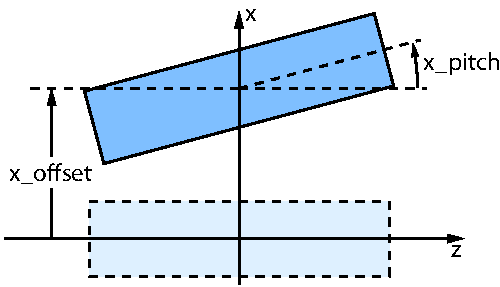
\includegraphics{pitch.pdf}
  \caption{Geometry of Pitch and Offset attributes}
  \label{f:pitch}
\end{figure}

\vn{x_offset} translates an element in the local $x$--direction
as shown in \fig{f:pitch}. Similarly, \vn{y_offset} and 
\vn{z_offset} translate an element along the local $y$ and 
$z$--directions respectively.

The \vn{x_pitch} attribute rotates an element about the element's
center such that the exit face of the element is displaced in the
$+x$--direction as shown in figure~\ref{f:pitch}.  An
\vn{x_pitch} represents a rotation around the positive $y$-axis.

Similarly, the \vn{y_pitch} attribute rotates an element about the
element's center using the negative $x$--axis as the rotation axis so
that the exit face of the element is displaced in the $+y$--direction.

The \vn{x_pitch} and \vn{y_pitch} rotations are about the center of
the element which is in contrast to the \vn{dtheta} and \vn{dphi}
misalignments of \mad which rotate around the entrance point. The
sense of the rotation between \bmad and MAD is:
\index{MAD!element rotation origin}
\begin{example}
  x_pitch (Bmad) =  dtheta (MAD)
  y_pitch (Bmad) = -dphi (MAD)
\end{example}

\begin{figure}[tb]
  \centering
  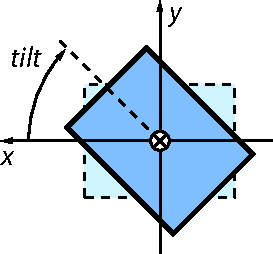
\includegraphics{tilt.pdf}
  \caption{Geometry of a Tilt}
  \label{f:tilt}
\end{figure}

The tilt attribute rotates the element in the $(x, y)$ plane as shown
in figure~\ref{f:tilt}. The rotation axis is the positive
$z$-axis. For example
\begin{example}
  q1: quad, l = 0.6, x_offset = 0.03, y_pitch = 0.001, tilt
\end{example}
\index{sol_quad!tilt default}\index{quadrupole!tilt default}
\index{sextupole!tilt default}\index{octupole!tilt default}
Like MAD, \bmad allows the use of the \vn{tilt} attribute without a
value to designate a skew element. The default tilt is $\pi/(2(n+1))$
where $n$ is the order of the element:
\begin{example}
  sol_quad       n = 1
  quadrupole     n = 1
  sextupole      n = 2
  octupole       n = 3
\end{example}

Note that \vn{hkick} and \vn{vkick} attributes are not affected by
\vn{tilt} except for \vn{kicker} and \vn{elseparator} elements.

%-----------------------------------------------------------------
\subsection{Bend Element Orientation}
\label{s:bend.orient}

\begin{figure}[ht]
  \centering
  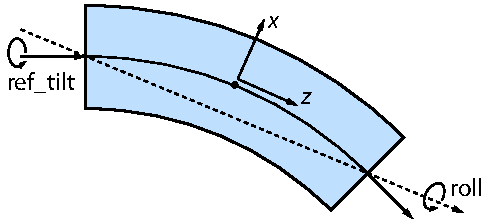
\includegraphics{roll.pdf}
  \caption[Geometry of a Bend]{
Geometry of a Bend. Like straight line elements, offsets and pitches
are calculated with respect to the coordinates at the center of the
bend. The exception is the \vn{roll} attribute which is a rotation
around the axis passing through the entrance and exit points.  Shown
here is the geometry for a bend with \vn{ref_tilt} = 0. That is, the bend
is in the $x-z$ plane.}
  \label{f:roll}
\end{figure}

The orientation attributes for \vn{sbend} and \vn{rbend} elements is
\begin{example}
  x_offset = <Real>
  y_offset = <Real>
  z_offset = <Real>
  x_pitch  = <Real>
  y_pitch  = <Real>
  ref_tilt = <Real>    ! Shifts and reference orbit rotation axis.
  roll     = <Real>    
\end{example}
The geometry for orienting a bend is shown in \fig{f:roll}. Like
straight line elements, the offset and pitch attributes are evaluated
with respect to the center of the element. 

Unlike the straight line elements, bends do not have a \vn{tilt}
attribute. Rather they have a \vn{ref_tilt} and a \vn{roll} attribute.
The \vn{roll} attribute rotates the bend along an axis that runs
through the entrance point and exit point as shown in
figure~\ref{f:roll}. A \vn{roll} attribute, like the offset and pitch
attributes does not affect the reference orbit.
The major effect of a \vn{roll} is to give a vertical
kick to the beam. For a bend with positive bend angle, a positive
\vn{roll} will move the outside portion ($+x$ side) of the bend upward
and the inside portion (-$x$ side) downward. Much like car racetracks
which are typically slanted towards the inside of a turn.

The \vn{ref_tilt} attribute of a bend rotates the bend about the $z$
axis at the upstream end of the bend as shown in \fig{f:roll}. Unlike
\vn{rolls} and \vn{tilts}, \vn{ref_tilt} also shifts the rotation axis
of the reference orbit along with the physical element. A \vn{bend}
with a \vn{ref_tilt} of $\pi/2$ will bend a beam vertically downward
(\sref{s:global}). Note that the \vn{ref_tilt} attribute of \bmad is
the same as the MAD \vn{tilt} attribute.

%-----------------------------------------------------------------
\subsection{Photon Reflecting Element Orientation}
\label{s:photon.orient}

\begin{figure}[ht]
  \centering
  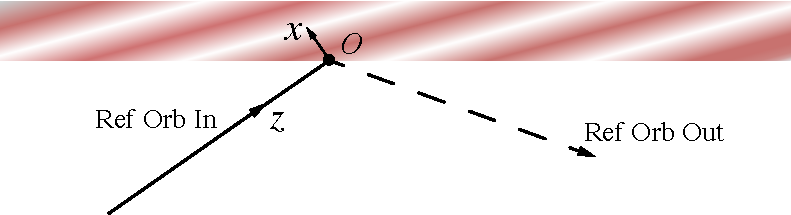
\includegraphics{reflect-orient.pdf}
  \caption[Geometry of a photon reflecting element orientation]{
Geometry of a photon reflecting element orientation.
The reference coordinates used for defining the orientational attribute
is the entrance reference coordinates. 
}
  \label{f:reflect.orient}
\end{figure}

Photon reflecting elements have the following orientational attributes:
\begin{example}
  x_offset = <Real>
  y_offset = <Real>
  z_offset = <Real>
  x_pitch  = <Real>
  y_pitch  = <Real>
  ref_tilt = <Real>    ! Shifts both element and reference orbit.
  tilt     = <Real>    
\end{example}
Roughly, these elements can be viewed as zero length bends except,
since there is no center position, the orientational attributes are
defined with respect to the entrance coordinates as shown in
\fig{f:reflect.orient}. Like bend elements, the \vn{ref_tilt} attribute
rotates both the physical element and the reference coordinates.
The \vn{tilt} attribute rotates just the physical element. Thus
the total rotation of the physical element about the entrance $z$
axis is the sum \vn{tilt} + \vn{ref_tilt}.

Frequently, it is desired to orient reflecting elements with respect
to the element's surface. This can be done using a \vn{girder} element
(\sref{s:girder}) which supports the reflecting element and with the
\vn{girder}'s \vn{origin_ele_ref_pt} attribute set to \vn{center}.

%-----------------------------------------------------------------
\subsection{Reference Orbit Manipulator Element Orientation}
\label{s:manip.orient}

The \vn{fork}, \vn{photon_fork}, \vn{floor_shift}, and \vn{patch} elements
use the following attributes to orient their exit edge with respect to their
entrance edge:
\begin{example}
  x_offset = <Real>
  y_offset = <Real>
  z_offset = <Real>
  x_pitch  = <Real>
  y_pitch  = <Real>
  tilt     = <Real>    
\end{example}
Here "exit" edge for \vn{fork} and \vn{photon_fork} elements is defined
to be the start of the line being branched to. [Within the line containing
the fork, the \vn{fork} element is considered to have zero length so the exit face
in the line containing the fork is coincident with the entrance face.]
The placement of the exit edge for these elements defines the reference orbit.
Thus, unlike the corresponding attributes for other elements, 
the orientational attributes here directly control the reference orbit.

%-----------------------------------------------------------------
\subsection{Fiducial Element Orientation}
\label{s:fiducial.orient}

The \vn{fiducial} element (\sref{s:girder}) uses the 
following attributes to define its position:
\begin{example}
  origin_ele        = <Name>     ! Reference element.
  origin_ele_ref_pt = <location> ! Reference pt on reference ele.
  dx_origin         = <Real>     ! x-position offset
  dy_origin         = <Real>     ! y-position offset
  dz_origin         = <Real>     ! z-position offset
  dtheta_origin     = <Real>     ! orientation angle offset.
  dphi_origin       = <Real>     ! orientation angle offset.
  dpsi_origin       = <Real>     ! orientation angle offset.
\end{example}
See Section~\sref{s:fiducial} for more details.

%-----------------------------------------------------------------
\subsection{Girder Orientation}
\label{s:girder.orient}

A \vn{girder} (\sref{s:girder}) element uses the same attributes as a \vn{fiducial}
element (\sref{s:fiducial}) to orient the reference girder position. In addition,
the following attributes are used to move the girder physically from the reference position: 
\begin{example}
  x_offset = <Real>
  y_offset = <Real>
  z_offset = <Real>
  x_pitch  = <Real>
  y_pitch  = <Real>
  tilt     = <Real>    
\end{example}
Shifting the girder from its reference position shifts all the elements that are
supported by the girder. See Section~\sref{s:girder} for more details.

\index{x_offset_tot|hyperbf}\index{y_offset_tot|hyperbf}\index{z_offset_tot|hyperbf}
\index{x_pitch_tot|hyperbf}\index{y_pitch_tot|hyperbf}
\index{tilt_tot|hyperbf}\index{roll_tot|hyperbf}\index{tilt_err_tot|hyperbf}
If an element is supported by a \vn{girder} element (\sref{s:girder}),
the orientational attributes of the element are with respect to the
orientation of the \vn{girder}. The computed offsets, pitches and tilt with
respect to the local reference coordinates are stored in the dependent attributes
\begin{example}
  x_offset_tot
  y_offset_tot
  z_offset_tot
  x_pitch_tot
  y_pitch_tot
  tilt_tot
  roll_tot
\end{example}
\index{sbend}\index{rbend}
A \vn{*_tot} attribute will only be present if the corresponding non
\vn{*_tot} attribute is present. For example, only \vn{sbend} and
\vn{rbend} elements have a \vn{roll_tot} attribute since only these
elements have a \vn{roll} attribute.

If an element is not supported by a \vn{girder}, the values of the
\vn{*_tot} attributes will be the same value as the values of the
corresponding non \vn{*_tot} attributes.

%-----------------------------------------------------------------
\section{Hkick, Vkick, and Kick Attributes}
\label{s:kick}
\index{hkick|hyperbf}\index{bl_hkick|hyperbf}
\index{vkick|hyperbf}\index{bl_vkick|hyperbf}
\index{kick|hyperbf}\index{bl_kick|hyperbf}


\index{hkicker}
\index{vkicker}
\index{elseparator}
\index{kicker}
The kick attributes that an element may have are:
\begin{example}
  kick,  bl_kick  = <Real>  ! Used only with a Hkicker or Vkicker
  hkick, bl_hkick = <Real>
  vkick, bl_vkick = <Real>
\end{example}
\vn{kick}, \vn{hkick}, and \vn{vkick} attributes are the integrated
kick of an element in radians. \vn{kick} is only used for \vn{hkicker}
and \vn{vkicker} elements. All other elements that can kick use
\vn{hkick} and \vn{vkick}. The \vn{tilt} attribute will only rotate a
kick for \vn{hkicker}, \vn{vkicker}, \vn{elseparator} and \vn{kicker}
elements. This rule was implemented so that, for example, the
\vn{hkick} attribute for a skew quadrupole would represent a
horizontal steering. The \vn{bl_kick}, \vn{bl_hkick}, and
\vn{bl_vkick} attributes are the integrated field kick in
\vn{meters-Tesla}. Normally these are dependent attributes except if
they appear in the lattice file (\sref{s:depend}).

For an \vn{elseparator} element, the \vn{hkick} and \vn{vkick} are
appropriate for a positively charged particle. The kick for a
negatively charged particle is opposite this.

%-----------------------------------------------------------------
\section{Aperture and Limit Attributes}
\label{s:limit}
\index{aperture|hyperbf}
\index{limit|hyperbf}
\index{aperture_at|hyperbf}

\begin{figure}[ht]
  \centering
  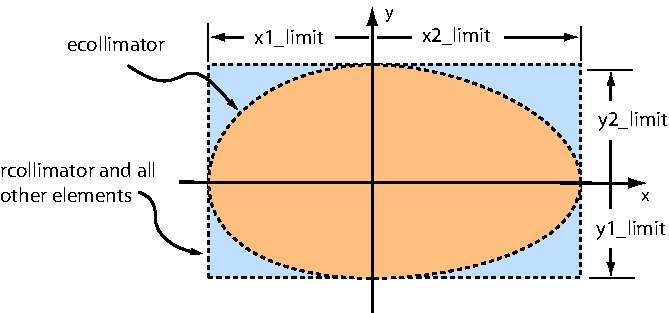
\includegraphics{apertures.pdf}
  \caption[Apertures for ecollimator and rcollimator elements.]
  {Apertures for ecollimator and rcollimator elements. 
  [note: positive $z$ points up, out of the page.] 
  As drawn, all limits \vn{x1_limit}, \vn{x2_limit}, 
  \vn{y1_limit}, \vn{y2_limit} are  positive.}  
  \label{f:limit}
\end{figure}

\index{ecollimator}
\index{rcollimator}
\index{x_limit|hyperbf}
\index{y_limit|hyperbf}
\index{x1_limit|hyperbf}
\index{y1_limit|hyperbf}
\index{x2_limit|hyperbf}
\index{y2_limit|hyperbf}
\index{x_offset|hyperbf}
\index{offset_moves_aperture|hyperbf}
\index{aperture_type}
The aperture attributes are:
\begin{example}
  x1_limit      = <Real>      ! Horizontal, negative side, aperture limit
  x2_limit      = <Real>      ! Horizontal, positive side, aperture limit
  y1_limit      = <Real>      ! Vertical, negative side, aperture limit
  y2_limit      = <Real>      ! Vertical, positive side, aperture limit
  x_limit       = <Real>      ! Alternative to specifying x1_limit and x2_limit
  y_limit       = <Real>      ! Alternative to specifying y1_limit and y2_limit
  aperture      = <Real>      ! Alternative to specifying x_limit and y_limit
  aperture_at   = <Switch>    ! What end aperture is at. (\sref{s:ap.place})
  aperture_type = <Switch>    ! What type of aperture it is
  offset_moves_aperture = <Logical> ! Element offsets affect aperture position (\sref{s:offset.ap})
\end{example}
\vn{x1_limit}, \vn{x2_limit}, \vn{y1_limit}, and \vn{y2_limit} specify
the half--width of the aperture of an element as shown in
figure~\ref{f:limit}. A zero \vn{x1_limit}, \vn{x2_limit},
\vn{y1_limit}, or \vn{y2_limit} is interpreted as no aperture in the
appropriate plane.

For convenience, \vn{x_limit} can be used to set \vn{x1_limit} and
\vn{x2_limit} to a common value. Example:
\begin{example}
  s: sextupole, x1_limit = 0.09, x2_limit = 0.09
  s: sextupole, x_limit = 0.09   ! Same as above
\end{example}
Similarly, \vn{y_limit} can be used
to set \vn{y1_limit} and \vn{y2_limit}.  The \vn{aperture} attribute
can be use to set all four \vn{x1_limit}, \vn{x2_limit}, \vn{y1_limit}
and \vn{y2_limit} to a common value. Internally, the \bmad code does {\em not}
store \vn{x_limit}, \vn{y_limit}, or \vn{aperture}. This means that
using \vn{x_limit}, \vn{y_limit} or aperture in arithmetic expressions is
an error:
\begin{example}
  q1: quad, aperture = 0.09         
  q2: quad, aperture = q1[aperture]   ! THIS IS AN ERROR!
  q2: quad, aperture = q1[x1_limit]   ! Correct
\end{example}

By default, apertures are assumed to be rectangular except that an
\vn{ecollimator} has a elliptical aperture. This can be changed by
setting the \vn{aperture_type} attribute. The possible values of this
attribute are:
\begin{example}
  auto         ! Default for detector, mask and diffraction_plate elements
  custom
  elliptical   ! Default for \vn{ecollimator} elements.
  rectangular  ! Default for most elements.
  wall3d       ! Vacuum chamber wall (\sref{s:wall}).
\end{example}
The \vn{custom} setting is used in the case where programs have been
compiled with custom, non-Bmad, code to handle the aperture
calculation.  The \vn{auto} setting is used for automatic calculation
of a rectangular aperture. For \vn{diffraction_plate} and \vn{mask}
elements, the \vn{auto} setting causes the four aperture limits to be
set to just cover the clear area of element
(\sref{s:masking.wall}). For all other elements, the \vn{auto}
setting is only to be used when there is an associated surface grid
(\sref{s:surf.grid}) for the element and, in this case, \bmad to set
the four limits to just cover the surface grid.

The \vn{wall3d} setting uses the vacuum chamber wall as specified by a \vn{wall} attribute
(\sref{s:wall}). Using the \vn{wall} construct allows for complex apertures to be
constructed. Note that The wall thickness and material type are not used when calculating
if a particle has hit the wall. That is, the wall is considered to be infinitely thin.
Also note that a wall must cover the entire length of the element longitudinally. This is done
in order to be able to spot errors in specifying the wall geometry.

For rectangular apertures, the limits \vn{x1_limit}, \vn{x2_limit},
\vn{y1_limit}, or \vn{y2_limit} may be negative. For example:
\begin{example}
  s: sextupole, x1_limit = -0.02, x2_limit = 0.09
\end{example}
In this case, particles will hit the aperture if their $x$-coordinate
is outside the interval [0.02, 0.09]. That is, particles at the origin
will be lost.

To avoid numerical overflow and other errors in tracking, a particle
will be considered to have hit an aperture in an element, even if
there are no apertures set for that element, if its orbit exceeds 1000
meters. Additionally, there are other situations where a particle will
be considered lost. For example, if a particle's trajectory does
not intersect the output face in a bend.

Examples:
\begin{example}
  q1, quadrupole, y1_limit = 0.03
  q1[y2_limit] = 0.03
  q1[y_limit] = 0.03  ! equivalent to the proceeding 2 lines.  
  q1[aperture_at] = both_ends
\end{example}

%-----------------------------------------------------------------
\subsection{Apertures and Element Offsets}
\label{s:offset.ap}

\index{tilt}
\index{x_offset}
\index{y_offset}
\index{x_pitch}
\index{y_pitch}
\index{rcollimator}\index{ecollimator}
\index{multilayer_mirror}\index{mirror}\index{crystal}
Normally, whether a particle hits an aperture or not is evaluated
independent of any element offsets (\sref{s:offset}). This is
equivalent to the situation where a beam pipe containing an aperture
is independent of the placement of the physical element the beam pipe
passes through. That is, the beam pipe does not ``touch'' the physical
element. This can be changed by setting the \vn{offset_moves_aperture}
attribute to \vn{True}. In this case any offsets or pitches will be
considered to have shifted the aperture boundary. The exceptions here
is that the default for the following elements is for
\vn{offset_moves_aperture} to be \vn{True}:
\begin{example}
  rcollimator, 
  ecollimator,
  multilayer_mirror, 
  mirror, and 
  crystal 
\end{example}

Even with \vn{offset_moves_aperture} set to \vn{True}, \vn{tilt}s will
not affect the aperture calculation. This is done, for example, so
that the tilt of a skew quadrupole does not affect the aperture. The
exception here is that tilting an \vn{rcollimator} or \vn{ecollimator}
element will tilt the aperture. Additionally, when the aperture is at
the \vn{surface} (see below), any \vn{tilt} will be used in the
calculation.

Example:
\begin{example}
  q1: quad, l = 0.6, x1_limit = 0.045, offset_moves_aperture = T
\end{example}

%-----------------------------------------------------------------
\subsection{Aperture Placement}
\label{s:ap.place}

\index{both_ends|hyperbf}\index{continuous|hyperbf}
\index{entrance_end|hyperbf}\index{exit_end|hyperbf}\index{wall_transition|hyperbf}
\index{surface|hyperbf}\index{aperture_at}\index{no_aperture}
By default, for most elements, the aperture is evaluated at the exit face of the
element. This can be changed by setting the \vn{aperture_at} attribute.
Possible settings for \vn{aperture_at} are:
\begin{example}
  both_ends
  continuous
  entrance_end
  exit_end       ! Default for most elements
  no_aperture
  surface  
  wall_transition
\end{example}
The \vn{exit_end} setting is the default for most elements except for
the following elements who have a default of \vn{surface}:
\index{mirror}\index{multilayer_mirror}\index{crystal}
\index{diffraction_plate}\index{sample}
\begin{example}
  crystal
  diffraction_plate
  mask
  mirror
  multilayer_mirror
  sample
\end{example}

In fact, for the following elements:
\begin{example}
  mirror, 
  multilayer_mirror
  crystal
\end{example}
The \vn{surface} setting for \vn{aperture_at} must be used.
Additionally, due to the complicated geometry of these elements, to
keep things conceptionally simple, the rule is imposed that, for an
aperture at the surface, the \vn{offset_moves_aperture} setting must
be left in its default state of True. Additionally, For
\vn{entrance_end} or \vn{exit_end} apertures,
\vn{offset_moves_aperture} must be set to False.

Note: The entrance and exit ends of an element are independent of which direction
particles are tracked through an element. Thus if a particle is tracked backwards it
enters an element at the ``exit end'' and exits at the ``entrance end''. The
\vn{continuous} setting indicates that the aperture is continuous along the length of the
element. This only matters when particle tracking involves stepping through an element a
little bit at a time. For example, as in Runge-Kutta tracking (\sref{s:tkm}). For tracking
where a formula is used to transform the particle coordinates at the entrance of an
element to the coordinates at the exit end, the aperture is only checked at the end points
so, in this situation, a \vn{continuous} aperture is equivalent to the \vn{both_ends}
setting.

The \vn{wall_transition} setting is like the \vn{continuous} setting in that the aperture
boundary is considered to be continuous along the element's length. However, unlike the
\vn{continuous} setting, with the \vn{wall_transition} setting a particle outside the wall
is considered alive and it is only when a particle moves through the wall that it is lost.
The \vn{wall_transition} setting is used for things like septum magnets where a particle
may be safely outside or inside the wall. Note to programmers: By supplying a custom
\vn{wall_hit_handler_custom} routine, scattering of particles through a wall may be
simulated.

Examples:
\begin{example}
  q2: quad, aperture_type = elliptical, aperture_at = continuous
  q1: quad, l = 0.6, x1_limit = 0.045, offset_moves_aperture = T
\end{example}

%-----------------------------------------------------------------
\subsection{Apertures and X-Ray Generation}
\label{s:aper.x.ray}

With X-ray simulation apertures can be used by \bmad to limit the
directions in which photons are generated. This can greatly decrease
simulation times. For example, a photon passing through a
\vn{diffraction_plate} element will diffract in an arbitrary
direction. If a {\em downstream} element has an aperture set, \bmad
can restrict the velocity directions so that the photons will fill the
downstream aperture and the amount of time wasted tracking photons
that ultimately would be collimated is minimal.

%-----------------------------------------------------------------
\section{X-Rays Crystal \& Compound Materials}
\label{s:cryst.list}

For basic crystallographic and X-ray matter interaction cross-sections,
\bmad uses the XRAYLIB\cite{b:xraylib} library. Crystal structure
parameters in XRAYLIB are mainly from R.~W.~G.~Wyckoff\cite{b:wyckoff}
with some structure parameters coming from NIST. The list of available
structures is:
\begin{center}
\begin{tabular}{llll} \toprule
AlphaAlumina & GaP       & KCl        & Platinum  \\
AlphaQuartz  & GaSb      & KTP        & RbAP      \\
Aluminum     & Ge        & LaB6       & Sapphire  \\
Be           & Gold      & LaB6_NIST  & Si        \\
Beryl        & Graphite  & LiF        & Si_NIST   \\
Copper       & InAs      & LiNbO3     & Si2       \\
CsCl         & InP       & Muscovite  & SiC       \\
CsF          & InSb      & NaCl       & Titanium  \\
Diamond      & Iron      & PET        & TlAP      \\
GaAs         & KAP       &            &           \\ \bottomrule
\end{tabular}
\end{center}
These names are case sensitive

Besides the above crystal list, \bmad can calculate structure factors
for all the elements and the following list of materials. Material
properties are from NIST. These names are case sensitive. That is, the
NIST materials all use upper case. As noted in the table, several of
the materials may be specified using the appropriate chemical
formula. For example, liquid water may be referenced using the name
\vn{H2O}.
\begin{center}
\footnotesize
\begin{longtable}{lll}
\multicolumn{3}{r}{{\normalsize Continued on next page}} \\
\endfoot
\endlastfoot
A_150_TISSUE_EQUIVALENT_PLASTIC     & LITHIUM_TETRABORATE                       \\
ACETONE                             & LUNG_ICRP                                 \\
ACETYLENE                           & M3_WAX                                    \\
ADENINE                             & MAGNESIUM_CARBONATE                       \\
ADIPOSE_TISSUE_ICRP                 & MAGNESIUM_FLUORIDE                        \\
AIR_DRY_NEAR_SEA_LEVEL              & MAGNESIUM_OXIDE                           \\
ALANINE                             & MAGNESIUM_TETRABORATE                     \\
ALUMINUM_OXIDE, Al2O3               & MERCURIC_IODIDE                           \\
AMBER                               & METHANE                                   \\
AMMONIA, NH3                        & METHANOL                                  \\
ANILINE                             & MIX_D_WAX                                 \\
ANTHRACENE                          & MS20_TISSUE_SUBSTITUTE                    \\
B_100_BONE_EQUIVALENT_PLASTIC       & MUSCLE_SKELETAL                           \\
BAKELITE                            & MUSCLE_STRIATED                           \\
BARIUM_FLUORIDE                     & MUSCLE_EQUIVALENT_LIQUID_WITH_SUCROSE     \\
BARIUM_SULFATE                      & MUSCLE_EQUIVALENT_LIQUID_WITHOUT_SUCROSE  \\
BENZENE, C6H6                       & NAPHTHALENE                               \\
BERYLLIUM_OXIDE                     & NITROBENZENE                              \\
BISMUTH_GERMANIUM_OXIDE             & NITROUS_OXIDE                             \\
BLOOD_ICRP                          & NYLON_DU_PONT_ELVAMIDE_8062               \\
BONE_COMPACT_ICRU                   & NYLON_TYPE_6_AND_TYPE_6_6                 \\
BONE_CORTICAL_ICRP                  & NYLON_TYPE_6_10                           \\
BORON_CARBIDE, B4C                  & NYLON_TYPE_11_RILSAN                      \\
BORON_OXIDE, B2O3                   & OCTANE_LIQUID                             \\
BRAIN_ICRP                          & PARAFFIN_WAX                              \\
BUTANE                              & N_PENTANE                                 \\
N_BUTYL_ALCOHOL                     & PHOTOGRAPHIC_EMULSION                     \\
C_552_AIR_EQUIVALENT_PLASTIC        & PLASTIC_SCINTILLATOR_VINYLTOLUENE_BASED   \\
CADMIUM_TELLURIDE                   & PLUTONIUM_DIOXIDE                         \\
CADMIUM_TUNGSTATE                   & POLYACRYLONITRILE                         \\
CALCIUM_CARBONATE                   & POLYCARBONATE_MAKROLON_LEXAN              \\
CALCIUM_FLUORIDE                    & POLYCHLOROSTYRENE                         \\
CALCIUM_OXIDE                       & POLYETHYLENE                              \\
CALCIUM_SULFATE                     & POLYETHYLENE_TEREPHTHALATE_MYLAR          \\
CALCIUM_TUNGSTATE                   & POLYMETHYL_METHACRALATE_LUCITE_PERSPEX    \\
CARBON_DIOXIDE                      & POLYOXYMETHYLENE                          \\
CARBON_TETRACHLORIDE                & POLYPROPYLENE                             \\
CELLULOSE_ACETATE_CELLOPHANE        & POLYSTYRENE                               \\
CELLULOSE_ACETATE_BUTYRATE          & POLYTETRAFLUOROETHYLENE_TEFLON            \\
CELLULOSE_NITRATE                   & POLYTRIFLUOROCHLOROETHYLENE               \\
CERIC_SULFATE_DOSIMETER_SOLUTION    & POLYVINYL_ACETATE                         \\
CESIUM_FLUORIDE                     & POLYVINYL_ALCOHOL                         \\
CESIUM_IODIDE                       & POLYVINYL_BUTYRAL                         \\
CHLOROBENZENE                       & POLYVINYL_CHLORIDE                        \\
CHLOROFORM                          & POLYVINYLIDENE_CHLORIDE_SARAN             \\
CONCRETE_PORTLAND                   & POLYVINYLIDENE_FLUORIDE                   \\
CYCLOHEXANE                         & POLYVINYL_PYRROLIDONE                     \\
12_DDIHLOROBENZENE                  & POTASSIUM_IODIDE                          \\
DICHLORODIETHYL_ETHER               & POTASSIUM_OXIDE                           \\
12_DICHLOROETHANE                   & PROPANE                                   \\
DIETHYL_ETHER                       & PROPANE_LIQUID                            \\
NN_DIMETHYL_FORMAMIDE               & N_PROPYL_ALCOHOL                          \\
DIMETHYL_SULFOXIDE                  & PYRIDINE                                  \\
ETHANE                              & RUBBER_BUTYL                              \\
ETHYL_ALCOHOL                       & RUBBER_NATURAL                            \\
ETHYL_CELLULOSE                     & RUBBER_NEOPRENE                           \\
ETHYLENE                            & SILICON_DIOXIDE                           \\
EYE_LENS_ICRP                       & SILVER_BROMIDE                            \\
FERRIC_OXIDE                        & SILVER_CHLORIDE                           \\
FERROBORIDE                         & SILVER_HALIDES_IN_PHOTOGRAPHIC_EMULSION   \\
FERROUS_OXIDE                       & SILVER_IODIDE                             \\
FERROUS_SULFATE_DOSIMETER_SOLUTION  & SKIN_ICRP                                 \\
FREON_12                            & SODIUM_CARBONATE                          \\
FREON_12B2                          & SODIUM_IODIDE                             \\
FREON_13                            & SODIUM_MONOXIDE                           \\
FREON_13B1                          & SODIUM_NITRATE                            \\
FREON_13I1                          & STILBENE                                  \\
GADOLINIUM_OXYSULFIDE               & SUCROSE                                   \\
GALLIUM_ARSENIDE                    & TERPHENYL                                 \\
GEL_IN_PHOTOGRAPHIC_EMULSION        & TESTES_ICRP                               \\
GLASS_PYREX                         & TETRACHLOROETHYLENE                       \\
GLASS_LEAD                          & THALLIUM_CHLORIDE                         \\
GLASS_PLATE                         & TISSUE_SOFT_ICRP                          \\
GLUCOSE                             & TISSUE_SOFT_ICRU_FOUR_COMPONENT           \\
GLUTAMINE                           & TISSUE_EQUIVALENT_GAS_METHANE_BASED       \\
GLYCEROL                            & TISSUE_EQUIVALENT_GAS_PROPANE_BASED       \\
GUANINE                             & TITANIUM_DIOXIDE                          \\
GYPSUM_PLASTER_OF_PARIS             & TOLUENE                                   \\
N_HEPTANE                           & TRICHLOROETHYLENE                         \\
N_HEXANE                            & TRIETHYL_PHOSPHATE                        \\
KAPTON_POLYIMIDE_FILM               & TUNGSTEN_HEXAFLUORIDE                     \\
LANTHANUM_OXYBROMIDE                & URANIUM_DICARBIDE                         \\
LANTHANUM_OXYSULFIDE                & URANIUM_MONOCARBIDE                       \\
LEAD_OXIDE                          & URANIUM_OXIDE                             \\
LITHIUM_AMIDE                       & UREA                                      \\
LITHIUM_CARBONATE                   & VALINE                                    \\
LITHIUM_FLUORIDE                    & VITON_FLUOROELASTOMER                     \\
LITHIUM_HYDRIDE                     & WATER_LIQUID, H2O                         \\
LITHIUM_IODIDE                      & WATER_VAPOR                               \\
LITHIUM_OXIDE                       & XYLENE                                    \\
\end{longtable}
\end{center}

%-----------------------------------------------------------------

\begin{figure}[tb]
  \centering
  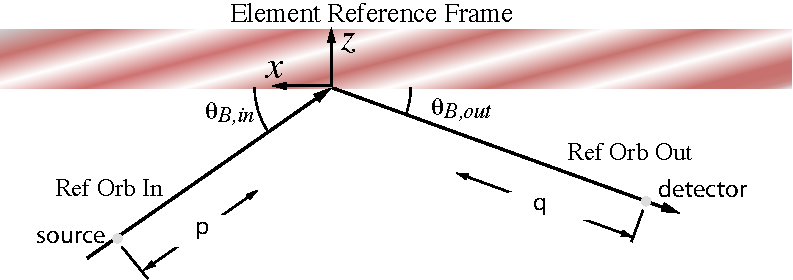
\includegraphics[width=5in]{surface-curvature.pdf}
  \caption[Surface curvature geometry.]
{Surface curvature geometry. The element reference frame used to
describe surface curvature has the $x$ axis pointing towards the
interior of the element, and the $z$ axis along the plane defined by
the entrance and exit reference orbit.}
  \label{f:surface}
\end{figure}

%-----------------------------------------------------------------
\section{Surface Properties for X-Ray elements}
\label{s:s.curve}

The following X-ray elements have a surface which X-rays impinge upon:
\begin{example}
  crystal               \sref{s:crystal}
  detector              \sref{s:detector}
  diffraction_plate     \sref{s:diff.plate}
  mask                  \sref{s:mask}
  mirror, and           \sref{s:mirror}
  multilayer_mirror     \sref{s:multilayer}
  sample                \sref{s:sample}
\end{example}
[There is also the \vn{capillary} element but this element specifies
its surface differently.]

The coordinate system used for characterizing the curvature of a
surface is the element reference frame as shown in
\fig{f:surface}). This coordinate system has the $x$ axis pointing
towards the interior of the element, and the $z$ axis along the plane
defined by the entrance and exit reference orbit. In this coordinate system, 
the surface curvature is parameterized by
a fourth order polynomial in $z$ and $y$
\Begineq
  {-z} = \sum_{2 \le i+j \le 6} c_{ij} \, x^i \, y^j
  \label{xs2ij4}
\Endeq
The coefficients are set in the lattice file by setting the following
element attributes
\index{surface curveture}
\begin{example}
  curvature_xM_yN      = <Real>   
\end{example}
where \vn{M} and \vn{N} are integers in the range 0 through 6 with the restriction
\begin{example}
  2 \(\le\) M + N \(\le\) 6
\end{example}
Example:
\begin{example}
  c2: crystal, curvature_x2_y0 = 37, ...
\end{example}
in this example, \vn{curvature_x2_y0} corresponds to the $c_{20}$ term
in \Eq{xs2ij4}. To get the effect of a nonzero $x^0\, y^0$, $x^1 \,
y^0$, or $x^0 \, y^1$ terms (since corresponding \vn{curvature_xN_yM}
are not permitted), element offsets and pitches can be used
(\sref{s:offset}).

Some useful formulas: Series expansion for a sphere of radius $R$:
\Begineq
  {-z} = \frac{x^2}{2 \, R} + \frac{x^4}{8 \, R^3} + \frac{x^6}{16 \, R^5} +
         \frac{y^2}{2 \, R} + \frac{y^4}{8 \, R^3} + \frac{y^6}{16 \, R^5} +
         \frac{x^2 \, y^2}{4 \, R^3} + \frac{3 \, x^4 \, y^2}{16 \, R^5} +
         \frac{3 \, x^2 \, y^4}{16 \, R^5} 
\Endeq
If $p$ is the distance from the source to the crystal, and $q$ is the
distance from the crystal to the detector, the radius of the Rowland
circle $R_s$ in the sagittal plane is given by\cite{b:del.rio}
\Begineq
  \frac{1}{p} + \frac{1}{q} = \frac{\sin\theta_{g,in} + \sin\theta_{g,out}}{R_s}
\Endeq
where $\theta_{g,in}$ and $\theta_{g,out}$ are the entrance and exit
graze angles. In the transverse plane (also called meridional plane),
the radius $R_t$ needed for foucusing is
\Begineq
  \frac{\sin^2\theta_{g,in}}{p} + \frac{\sin^2\theta_{g,out}}{q} = \frac{\sin\theta_{g,in} + \sin\theta_{g,out}}{R_t}
\Endeq

Example:
\begin{example}
  t_bragg = 1.3950647
  rt = 1  ! Crystal transverse radius
  rs = rt*(sin(t_bragg))^2
  c: crystal, crystal_type =  'Si(553)', b_param = -1,
        curvature_x0_y2 =  1 / (2 * rs), curvature_x0_y4 = 1 / (8 * rs^3),
        curvature_x2_y0 = 1 / (2 * rt), curvature_x4_y0 = 1 / (8 * rt^3),
\end{example}

%-----------------------------------------------------------------
\subsection{Surface Grid}
\label{s:surf.grid}
\index{surface grid}

A surface can be broken up into a grid of rectangles. This is useful,
for example, in breaking up a \vn{detector} element into pixel photo
receptors or in simulating a rough serface for \vn{crystal}s and other
elements. The general syntax is:
\begin{example}
  surface = \{
    grid = \{                
      type = <type_name>,                ! Crystals: Off, Segmented, or H_Misalign
      ix_bounds = (<ix_min>, <ix_max>),  ! Min/max index bounds in x-direction
      iy_bounds = (<iy_min>, <iy_max>),  ! Min/max index bounds in y-direction
      r0 = (<x0>, <y0>),                 ! (x,y) coordinates at grid origin
      dr = (<dx>, <dy>),                 ! width and height of pixels.
      pt(<i>,<j>) = (<x_pitch>, <y_pitch>, <x_pitch_rms>, <x_pitch_rms>),
          \} \}
\end{example}
Example:
\begin{example}
  ccd: crystal, surface = \{
          grid = \{
            type = h_misalign,
            r0 = (0.0, 0.01), dr = (0.005, 0.005),
            ix_bounds = (1, 57), iy_bounds = (-30, 10),
            pt(1,-30) = (0.001, -0.002, 0, 0), 
            pt(1,-29) = ..., 
          \} \}
\end{example}

The grid is a two dimensional with bounds given by the \vn{ix_bounds}
and \vn{iy_bounds} components. These two components must be present. In
the above example the grid is 57 pixels in $x$ and 41 pixels in $y$.

The physical placement of the grid on the element is determined by the
\vn{r0} and \vn{dr} components. \vn{r0} is optional and gives the
$(x,y)$ coordinates of the center of the pixel with index $(0,0)$. The
\vn{dr} component, which must be present, gives the pixal width and
height. Thus the center of the $(i,j)$ pixel is:
\begin{example}
  (x,y) = (r0(1), r0(2)) + (i*dr(1), j*dr(2))
\end{example}

The \vn{type} component of the grid is used for
\vn{crystal} elements only. Possible \vn{type} values are:
\begin{example}
  H_Misalign         ! Misalignment of crystal H vector
  Off                ! Ignore grid
  Segmented          ! Surface is a matrix of flat rectangles
\end{example}
\vn{H_Misalign} misaligns the $H$ vector which is the normal to the
diffracting planes of the the crystal (\sref{s:crystal.tracking}).
When using \vn{H_Misalign}, each \vn{pt(i,j)} component gives the
misalignment of $H$ for the corresponding pixel. For an individual
photon, the misalignt of $H$ will be
\begin{example}
  x_pitch_tot = <x_pitch> + r1 * <x_pitch_rms>
  y_pitch_tot = <y_pitch> + r2 * <y_pitch_rms>
\end{example}
where \vn{x_pitch_tot} and \vn{y_pitch_tot} are the rotational
misalignment (\sref{s:offset}) used in the calculation, the quantities
in brackets \vn{<...>} are components of \vn{pt}, and \vn{r1} and
\vn{r2} are Gaussian distributed random numbers with unit rms. These
random numbers are regenerated for each photon. Note: \vn{pt} is only
used with \vn{H_Misalign}.

When the \vn{type} component is set to \vn{Segmented}, the crystal
surface is modeled as a grid of flat ``rectangles'' (the actual shape
is very close but not quite rectangular). Using a segmented crystal
only makes sense when the crystal is curved. There is one rectangle
for each pixel. Each rectangle has an extent in the $(x,y)$ transverse
dimensions equal to the extent of the corresponding pixel. The $z$
coordinate of the vertices of the rectangular are adjusted so that 
\begin{example}
  1) The rectangle is flat
  2) The rectangle contacts the unsegmented surface two diagonally opposite vertices.
  3) The other two diagonnaly opposite vertices will be as close as possible in the
     least squares sense from the unsegmented surface.
\end{example}

When the \vn{type} component is set to \vn{Off}, the grid will not be used.

%-----------------------------------------------------------------
\section{Walls: Vacuum Chamber, Capillary and Mask}
\label{s:wall}
\index{wall}

The \vn{wall} attribute for an element is used to define:
\begin{example}
  vacuum chamber wall
  capillary element (\sref{s:capillary}) inside wall
  diffraction_plate (\sref{s:diff.plate}) geometry
\end{example}

The topics of the following subsections are:
\begin{example}
  \sref{s:wall.syntax}      General wall syntax.
  \sref{s:wall.section}      Cross-section construction. 
  \sref{s:wall.interpolation}      Capillary and vacuum chamber wall interpolation.
  \sref{s:wall.capillary}      Capillary wall.
  \sref{s:wall.vacuum}      Vacuum chamber wall.
  \sref{s:masking.wall}      Mask wall for diffraction_plate and mask elements.
\end{example}

%-----------------------------------------------------------------
\subsection{Wall Syntax}
\label{s:wall.syntax}

The syntax of the \vn{wall} attribute is:
\begin{example}
  wall = \{
    superimpose = <T/F>,               ! Chamber wall only
    thickness = <real>                 ! Default thickness. 
    opaque_material = <material_type>  ! Default opaque material. 
    clear_material = <material_type>   ! Default clear material. 
    section = \{ 
      type = <section_type>,           ! Chamber Mask, and Diffraction_plate only
      s = <longitudinal_position>,     ! Relative to beginning of element.
      r0 = (<x0>, <y0>),               ! section (x,y) origin
      absolute_vertices = <T/F>,       ! Vertex nums: abs or relative to r0? Default = F.
      material = <material_type>,      ! Mask and Diffraction_plate only.
      thickness = <real>,              ! Mask and Diffraction_plate only.
      dr_ds = <value>,                 ! Capillary and Chamber only
      v(1) = \{<x>, <y>, <radius_x>, <radius_y>, <tilt>\}, 
      v(2) = \{ ... \},
      ...\},
    section = \{
      s = <longitudinal_position>, 
      v(1) = \{... \},
      ... \},
    ... \}
\end{example}
A \vn{wall} begins with ``\vn{wall = \{}'' and ends with a
``\vn{\}}''. In between are a number of individual cross-section
structures. Each individual cross-section begins with ``\vn{section =
\{}'' and ends with a ``\vn{\}}''. The \vn{s} parameter of a
cross-section gives the longitudinal position of the cross-section.
Example:
\begin{example}
  this_cap: capillary, 
    wall = \{   
      section = \{ ! cross-section with top/bottom symmetry
        s = 0, v(1) =  \{0.02, 0.00\}, 
        v(2) = \{0.00, 0.02, 0.02\}, v(3) = \{-0.01, 0.01\} \}, 
      section = \{  ! Cross-section that is a tilted ellipse.
        s = 0.34, 
        v(1) = \{0.003, -0.001, 0.015, 0.008, 0.2*pi\} \} \}
\end{example}
In this example an element called \vn{this_cap} is a \vn{capillary}
whose wall is defined by two cross-sections.

%------------------

\begin{figure}[tb]
  \centering
  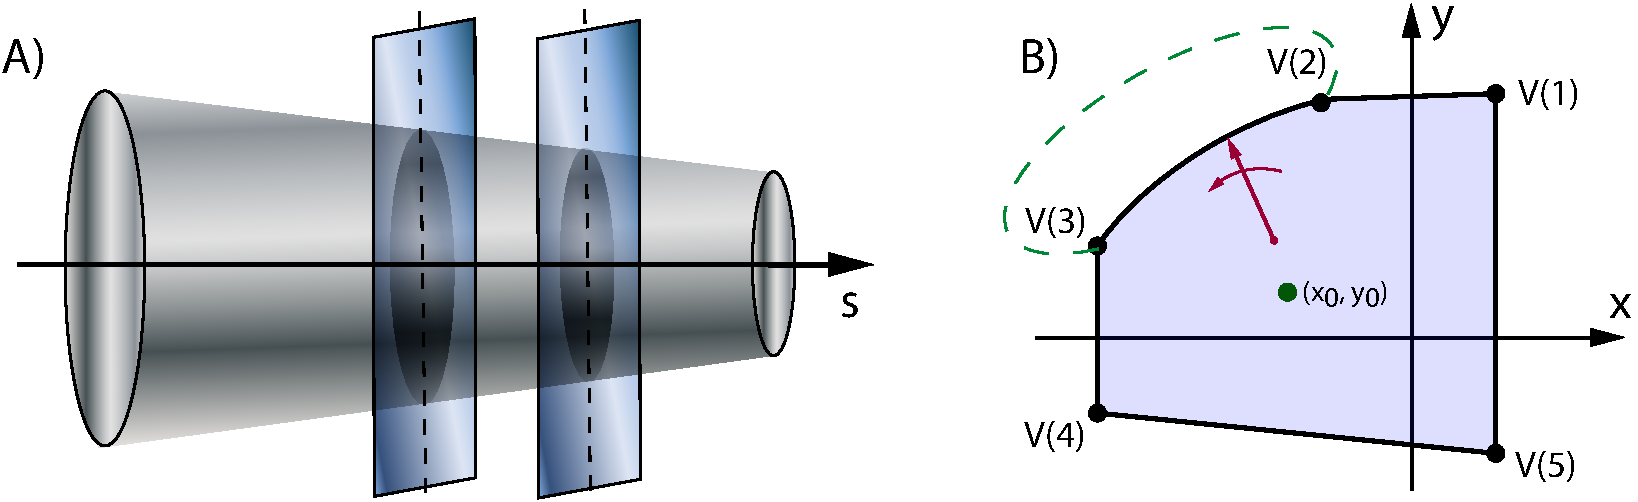
\includegraphics[width=6in]{chamber-wall.pdf}
  \caption[Capillary or vacuum chamber wall.]
{A) The inside wall of a capillary or the vacuum chamber wall of a
non-capillary element is defined by a number of cross-sectional
slices.  B) Each cross-section is made up of a number of vertices. The
segments between the vertices can be either a line segment, the arc of
a circle, or a section of an ellipse.}
  \label{f:chamber.wall}
\end{figure}

%-----------------------------------------------------------------
\subsection{Wall Sections}
\label{s:wall.section}

The wall is defined by a number of cross-sectional slices. For
\fig{f:chamber.wall}A shows the geometry for \vn{capillary} or vacuum
chamber walls.  Each cross-section is defined by a longitudinal
position $s$ relative to the beginning of the element and a number of
vertices. The verticies are defined with respect to the local sector
origin $r_0$ except if \vn{absolute_vertices} is set to \vn{True} in
which case the vertex numbers are taken as absolute. The arc between
each vertex may be either a straight line, an arc of a circle, or a
section of an ellipse. For a capillary it is mandatory that a
cross-section be convex. That is, given any two points within the
cross-section, all points on the line segment connecting them must be
within the cross-section.

The \vn{v(<j>)} within a cross-section define the vertices for each
cross-section. The vertices are defined with respect to the section
origin given by \vn{r0}. Each \vn{v(<j>)} has five
parameters. It is mandatory to specify the first two parameters
\vn{<x>} and \vn{<y>}. Specifying the rest, \vn{<radius_x>},
\vn{<radius_y>}, and \vn{<tilt>}, is optional. The default values, if
not specified, is zero. The point (\vn{<x>}, \vn{<y>}) defines the
position of the vertex. The parameters \vn{<radius_x>},
\vn{<radius_y>}, and \vn{<tilt>} define the shape of the segment of
the cross-section between the given vertex and the preceding one.
\begin{example}
  <radius_x>  = 0, <radius_y>  = 0   --> Straight line segment.
  <radius_x> != 0, <radius_y>  = 0   --> Circular arc with radius = radius_x
  <radius_x>  = 0, <radius_y> != 0   --> Illegal!
  <radius_x> != 0, <radius_y> != 0   --> Ellipse section.
\end{example}
When an ellipse is specified, \vn{<radius_x>}, and \vn{<radius_y>} are
the half width and half height of the semi-major axes and the
\vn{<tilt>} parameter gives the tilt of the ellipse. \vn{<radius_x>}
and \vn{<radius_y>} must not be negative.

In the example above, for the first cross-section, \vn{v(2)}
specifies a non-zero \vn{<radius_x>} and, by default, \vn{<radius_y>}
is zero. Thus the segment of the cross-section between \vn{v(1)} and
\vn{v(2)} is circular in nature with a radius of 0.02. Since \vn{v(3)}
does not specify \vn{<radius_x>} nor \vn{<radius_y>}, the
cross-section between \vn{v(2)} and \vn{v(3)} is a straight line
segment.

The vertex points must be arranged in a ``counter clockwise manner''. 
For vertices \vn{<v(i)>} and \vn{<v(i+1)>} connected by a line segment
this translates to
\Begineq
  0 < \theta_{i+1} - \theta_{i} \pmod{2\pi} < \pi
\Endeq
where $(r_n, \theta_n)$ are the polar coordinates of the $n^{th}$
vertex. For vertices connected by an arc, ``counter clockwise manner''
means that the line segment with one end at the center of the arc and
the other end traversing the arc from \vn{<v(i)>} to \vn{<v(i+1)>}
rotates in counter clockwise as shown in
\fig{f:chamber.wall}B. 

The red line segment with one end at the center of the arc and the
other end traversing the arc from, in this case, $V(2)$ to $V(3)$,
rotates in counter clockwise manner. In general, there are two
solutions for constructing such an arc. For positive radii, the
solution chosen is the one whose center is closest to the section
origin $(x_0, y_0)$. If the radii are negative, the center point will
be the point farthest from the origin (the dashed line between $V(2)$
and $V(3)$ in the figure).

A restriction on cross-sections is that the section origin $(x_0,
y_0)$ must be in the interior of any cross-section and that for any
cross-section a line drawn from the origin at any given angle $\theta$
will intersect the cross-section at exactly one point as shown in
\fig{f:chamber.wall}B. This is an important point in the construction
of the wall between cross-sections as explained below.

The last vertex specified, call it \vn{<v(n)>}, should not have the
same \vn{<x>}, \vn{<y>} values as the first vertex \vn{<v(1)>}. That
is, there will be a segment of the cross-section connecting
\vn{<v(n)>} to \vn{<v(1)>}. The geometry of this segment is determined
by the parameters of \vn{<v(1)>}.

If there is mirror symmetry about the $x$ or $y$ axis for a
cross-section, the ``mirrored'' vertices, on the ``negative'' side of
the mirror plane, do not have to be specified. Thus if all the vertex
points of a cross-section are in the first quadrant, that is, all
\vn{<x>} and \vn{<y>} are zero or positive, mirror symmetry about both
the $x$ and $y$ axes is assumed. If all the \vn{<y>} values are zero
or positive and some \vn{<x>} values are positive and some are
negative, mirror symmetry about the $x$ axis is assumed. Finally, if
all the \vn{<x>} values are zero or positive but some \vn{<y>} values
are positive and some are negative, symmetry about the $y$ axis is
assumed. For example, for the first in the above example, since all
the \vn{<y>} values are non-negative and there are positive and
negative \vn{<x>} values, symmetry about the $x$ axis is assumed.

The one exception to the above rule that (\vn{<x>}, \vn{<y>}) is the
vertex center is when a single vertex \vn{v(1)} is specified for a
cross-section with a non-zero \vn{<radius_x>}. In this case,
(\vn{<x>}, \vn{<y>}) are taken to be the center of the circle or
ellipse. For example, if a single vertex is specified for a
cross-section as:
\begin{example}
  section = \{s = 0.3, v(1) = \{0.03, -0.01, 0.15, 0.08, 0.2\}\}
\end{example}
the cross-section will be an ellipse with center at $(0.03, -0.01)$
with a tilt of $0.2$ and axes radii of $0.15$ and $0.08$. If
a cross-section has a single vertex and \vn{<radius_x>} is not
specified, the cross-section is a rectangle. For example
\begin{example}
  section = \{s = 0.3, v(1) = \{0.03, 0.01\}\}
\end{example}

%-----------------------------------------------------------------
\subsection{Interpolation Between Sections}
\label{s:wall.interpolation}

\begin{figure}[tb]
  \centering
  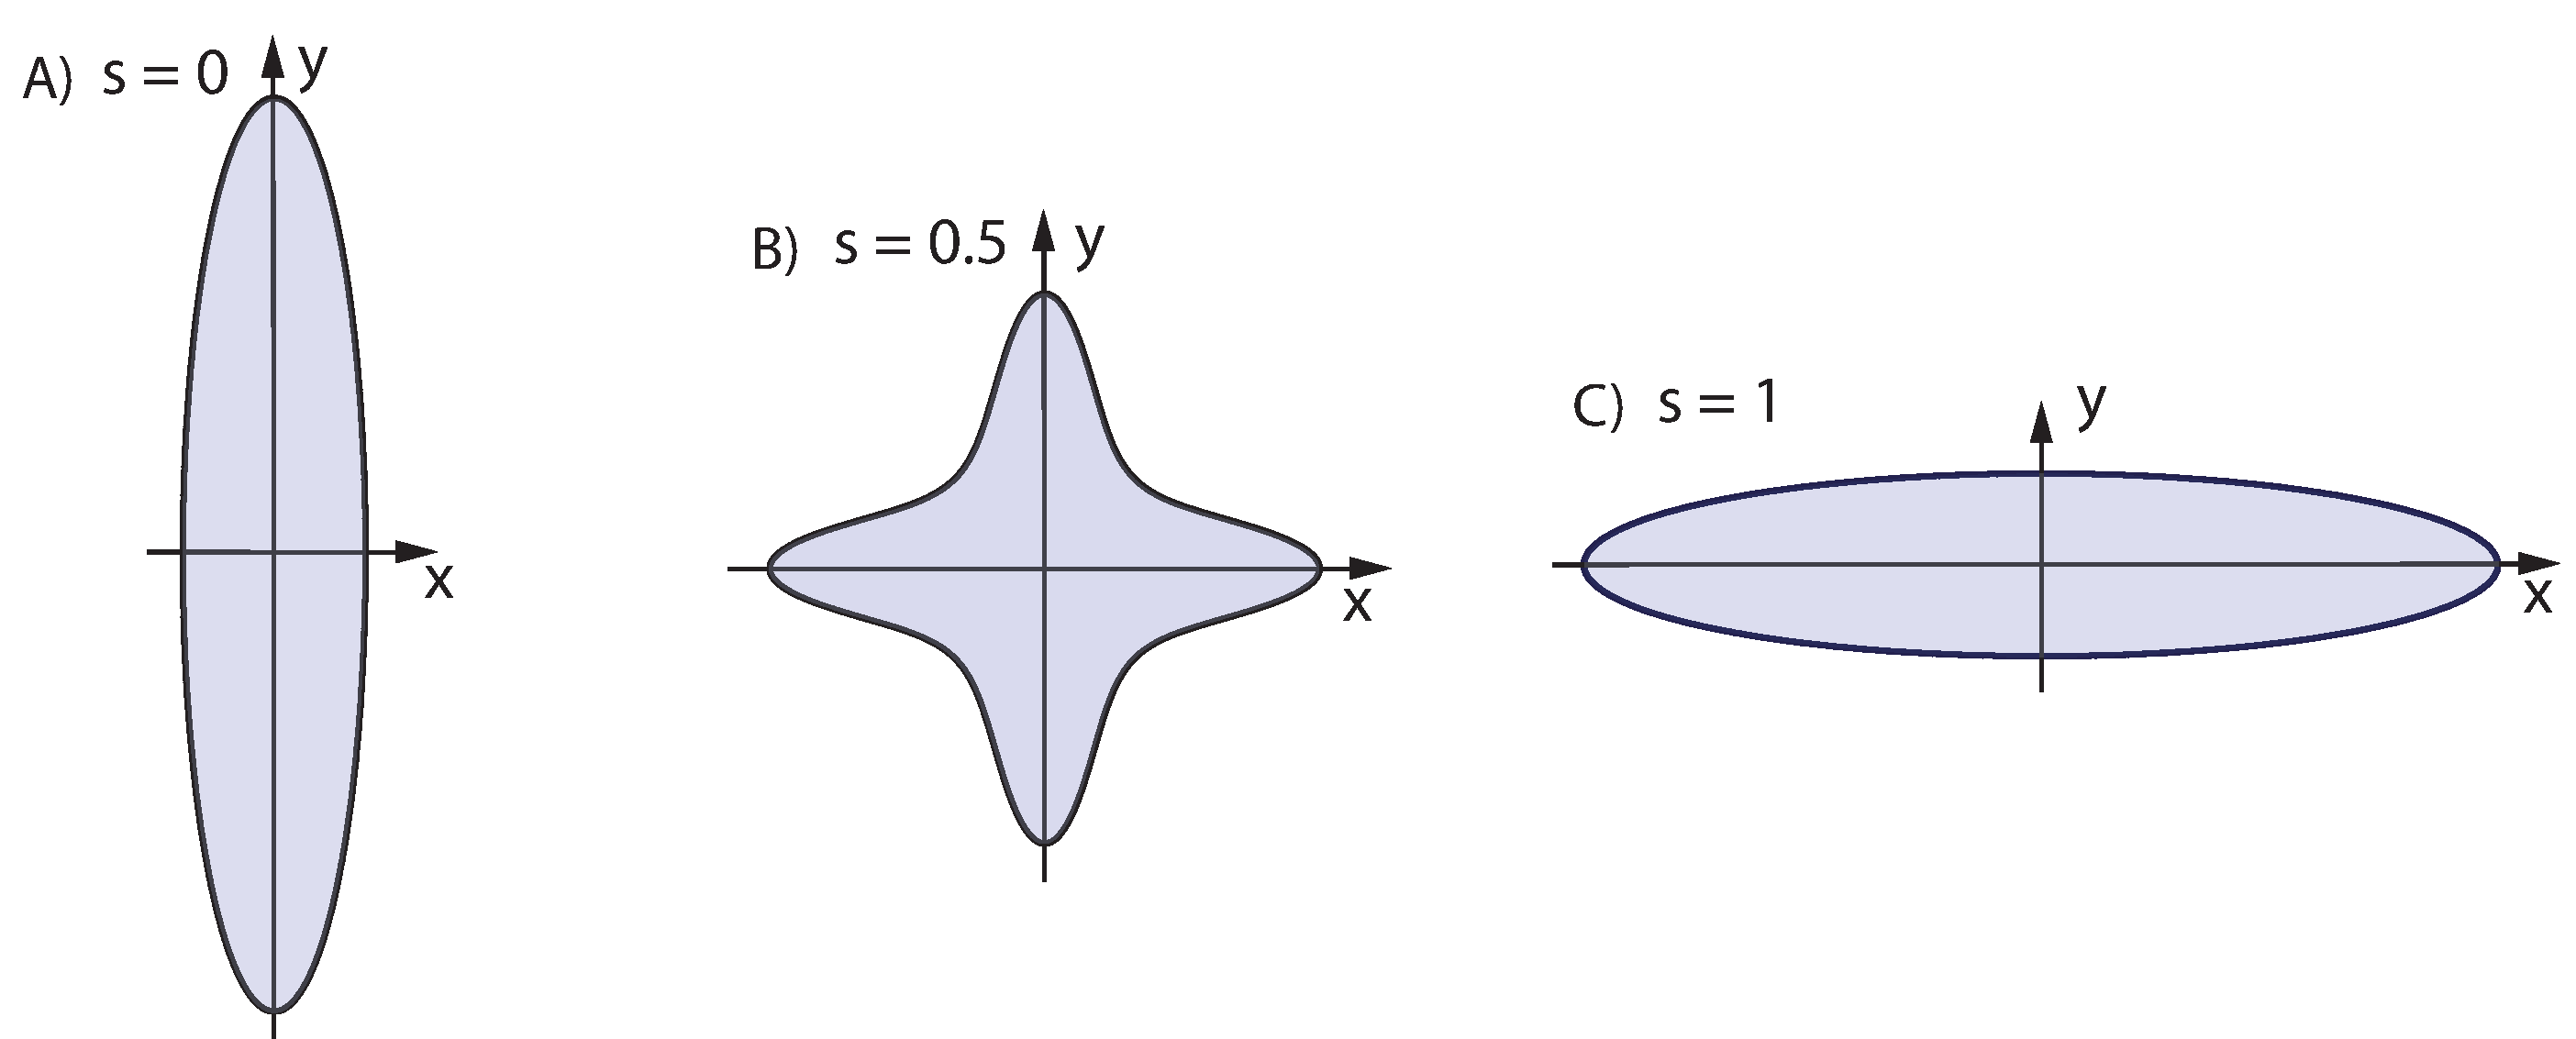
\includegraphics[width=4in]{concave-capillary.pdf}
  \caption[Convex cross-sections do not guarantee a convex volume.]
{Example where convex cross-sections do not produce a convex volume.
Cross-sections (A) and (C) are ellipses with a 5 to 1 aspect ratio.
Half way in between, linear interpolation produces a convex cross-section
as shown in (B).} 
  \label{f:concave.capillary}
\end{figure}

For \vn{capillary} and vacuum chamber walls, the wall between
cross-sections, is defined by interpolation. At a given $s$ position,
the $r, \theta$ coordinate system in the transverse $x, y$ plane is
defined with respect to an origin $\bfr_O(s)$ given by a linear
interpolaion of the origins of the cross-sections to either side of the
given $s$ position. Let $s_1$ denote the position of the cross-section
just before $s$ and $s_2$ denote the position of the cross-section
just after $s$. Let $\bfr_{01}$ be the $(x_0, y_0)$ origin defined
for the cross section at $s_1$ and $\bfr_{02}$ be the $(x_0, y_0)$
origin defined for the cross section at $s_2$. Then
\Begineq
  \bfr_O(s) = (1 - \stilde) \, \bfr_{01} + \stilde \, \bfr_{02}
\Endeq
where 
\Begineq
  \stilde \equiv \frac{s - s_1}{s_2 - s_1}
\Endeq

Let $r_{c1}(\theta)$ and $r_{c2}(\theta)$ be the radiusus of the wall
as a function of $\theta$ for the cross-sections at $s = s_1$ and $s =
s_2$ respectively. The wall $r_c(\theta, s)$ at any point $s$ between
$s_1$ and $s_2$ is then defined by the equation
\Begineq
  r_c(\theta, s) = p_1(\stilde) \, r_{c1}(\theta) + p_2(\stilde) \, r_{c2}(\theta)
\Endeq
where $p_1$ and $p_2$ are cubic polynomials parameterized by
\begin{align}
  p_1 &= 1 - \stilde + a_1 \, \stilde + a_2 \, \stilde^2 + a_3 \, \stilde^3 \CRNO
  p_2 &= \stilde + b_1 \, \stilde + b_2 \, \stilde^2 + b_3 \, \stilde^3 
\end{align}
If $a_i = b_i = 0$ for all $i = 1, 2, 3$, the interpolation is linear
and this is the default if either of the parameters \vn{dr_ds1} and
\vn{dr_ds2} are not given in the wall definition. These parameters are
the slopes of the wall with respect to $s$ at the end points
\begin{equation}
  \text{dr_ds1} \equiv \left. \frac{d\overline{r}}{ds} \right|_{s = s_1} \comma \qquad
  \text{dr_ds2} \equiv \left. \frac{d\overline{r}}{ds} \right|_{s = s_2} 
\end{equation}
where $\overline{r}$ is the average $r$ averaged over all
$\theta$. When {\em both} \vn{dr_ds1} and \vn{dr_ds2} are specified, the $a_i$
and $b_i$ are calculated so that the slopes of the wall match 
the values of \vn{dr_ds1} and \vn{dr_ds2} along with the constraints.
\begin{align}
  p_1(0) &= 1 \comma \qquad p_1(1) = 0 \CRNO
  p_2(0) &= 0 \comma \qquad p_2(1) = 1 \\
  M &\equiv a_1^2 + a_2^2 + a_3^2 + b_1^2 + b_2^2 + b_3^2 \text{ is a minimum}
  \nonumber
\end{align}
The last constraint ensures a ``smooth'' transition between the two cross-sections.

To refer to a cross-section parameters after an element has been
defined, the following syntax is used:
\begin{example}
  ele_name[wall%section(n)%v(j)%x]   ! x value of j^th vertex of n^th cross-section
\end{example}

%-----------------------------------------------------------------
\subsection{Capillary Wall}
\label{s:wall.capillary}
\index{capillary!wall}

For a \vn{capillary}, \vn{s} must be zero for the first cross-section and
the length of the capillary is given by the value of \vn{s} of the
last cross-section.

For a \vn{capillary}, in order for \bmad to quickly track photons,
\bmad assumes that the volume between the cross-sections is
convex. The volume will be convex if each cross-section $r_c(\theta,
s)$ at any given $s$ is convex. Note that it is {\em not} sufficient
for $r_c(\theta, s)$ to be convex at the specified cross-sections as
shown in \fig{f:concave.capillary}. Also note that it is perfectly
fine for the total capillary volume to not be convex.

%-----------------------------------------------------------------
\subsection{Vacuum Chamber Wall}
\label{s:wall.vacuum}

The vacuum chamber wall is independent of the element apertures
(\sref{s:limit}). Unless a program is specifically constructed, the
presence of a vacuum chamber wall will not affect particle tracking.

The vacuum chamber wall defined for an element may be shorter or
longer than the element.  The vacuum chamber wall for a particular
lattice branch is the sum of all the chamber walls of the individual
elements. That is, the chamber wall at any given point is determined
by interpolation of the nearest sections upstream and downstream to
the point.  Thus a given lattice element need not contain a \vn{wall}
component for the chamber wall to be well defined at the element. 

The exception to the above rule is when a \vn{section} has its
\vn{type} component set to either:
\begin{example}
  wall_start
  wall_end
\end{example}
\vn{wall_start} and \vn{wall_end} sections must come in pairs. The
next section after a \vn{wall_end} section (if this section is not
the last section in the lattice) must be a \vn{wall_start} section.
If a section has a \vn{type} of \vn{wall_start}, the region between
that section and the previous section (which must be a \vn{wall_end}
section) will be considered to have no wall. If the \vn{wall_start}
section is the first section of the lattice branch, the region of no
wall will start at the beginning of the branch. Similarly, if a
section has a \vn{type} of \vn{wall_end}, the region between that
section and the next section (or the end of the lattice branch if
there is no next seciton) will not have a wall.

The chamber walls of any two elements may not overlap. The exception
is when the \vn{superimpose} attribute for a wall of an element is set
to True. In this case, any other wall cross-sections from any other
elements that overlap the superimposed wall are discarded.
Superposition of a wall is useful, for example, in introducing mask
regions into the wall.

If a branch has a closed geometry (\sref{s:param}), wall sections that
extend beyound the ends of the branch are ``wrapped'' around.

If a particle is past the last wall cross-section or before the first
wall cross-section, The following rules are used: If the branch has a
\vn{closed geometry}, the wall will be interpolated between the last
and first cross-sections. If the branch has an \vn{open} geometry, the
wall is taken to have a constant cross-section in these regions. 

The chamber wall is defined with respect to the local coordinate
system (\sref{s:ref}). That is, in a bend a wall that has a constant
cross section is a section of a torus.

\index{patch!and chamber wall}
\vn{Patch} elements (\sref{s:patch}) complicate the wall geometry
since the coordinate system at the end of the \vn{patch} may be
arbitrarily located relative to the beginning of the patch. To avoid
confusion as to what coordinate system a wall section belongs to,
\vn{patch} elements are not allowed to define a wall. The wall through
a patch is determined by the closest wall sections of neighboring
elements.

%-------------------

\begin{figure}[tb]
  \centering
  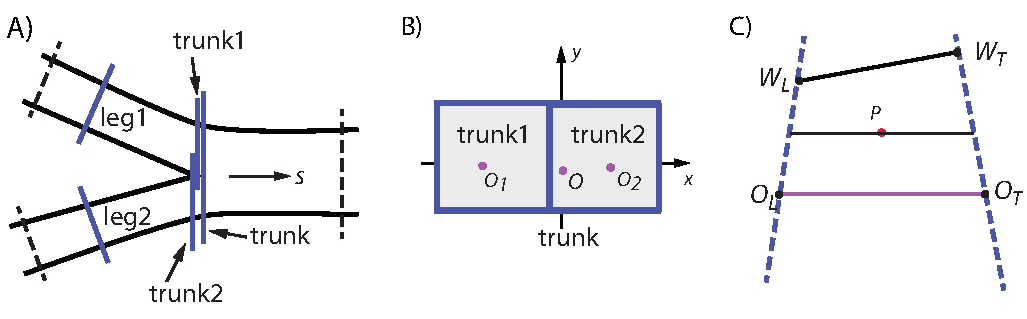
\includegraphics[width=6in]{crotch.pdf}
  \caption[vacuum chamber crotch geometry.]
{A) Crotch geometry: Two pipes labeled ``leg1'' and ``leg2'' merge
into a single pipe called the ``trunk'' pipe. Five wall sections are
used to define the crotch geometry (solid lines). Dashed lines
represent sections not involved in defining the crotch. For purposes
of illustration, the three trunk sections are displaced longitudinally
but in reality must have the same longitudinal coordinate.  B) Example
layout of the trunk1, trunk2 and trunk wall sections. $O_1$, $O_2$
and $O$ are the $x_0, y_0$ origins of the sections.}
  \label{f:crotch}
\end{figure}

%-------------------

\index{crotch chamber geometry}
Each section has a \vn{type} attribute. This attribute is not used for 
\vn{capillary} elements. For a vacuum chamber wall, the \vn{type} 
attribute is used to dscribe a ``crotch'' geometry where
two pipes merge into one pipe. The possible values for the \vn{type} 
attribute are:
\begin{example}
  normal     ! default
  leg1
  leg2
  trunk1
  trunk2
  trunk
\end{example}
The geometry of a crotch is shown in \fig{f:crotch}A. Two pipes,
called ``leg1'' and ``leg2'', merge into one pipe called the ``trunk''
pipe.  The trunk pipe can be either upstream or downstream of the leg
pipes.  To describe this situation, five sections are needed: One
section in each leg pipe which need to have their \vn{type} attribute
set to \vn{leg1} and \vn{leg2}, and three sections in the trunk with
one having a a \vn{type} attribute of \vn{trunk1}, another having a
\vn{type} attribute of \vn{trunk2} and the third haveing a \vn{type}
attribute of \vn{trunk}. There can be no sections between the leg
sections and the trunk sections.

All three trunk sections must be associated with the same element and
have the same \vn{s} value. In the list of sections of the element
containing the trunk elements, the \vn{trunk1} and \vn{trunk2}
sections must be listed first if the leg pipes are upstream of the
trunk pipe (the situation shown in the figure) and must be listed last
if the leg pipes are downstream. That is, the \vn{trunk1} and
\vn{trunk2} sections are ``between'' the leg sections and the
\vn{trunk} section. It does not matter if \vn{trunk1} is before or
after \vn{trunk2}.

The \vn{trunk1} and \vn{trunk2} sections must not overlap and the
\vn{trunk} section must be constructed so that its area is the union
of the areas of \vn{trunk1} and \vn{trunk2}. An example is illustrated
in \fig{f:crotch}B. Here the \vn{trunk1} and \vn{trunk2} sections are
squares with origins labeled $O_1$ and $O_2$ in the figure. By
necessity, these origins must be different since each must lie within
the boundaries of their respective areas. The \vn{trunk} section is a
rectagle encomposing the two squares and has an origin labeled $O$.

Between \vn{leg1} and \vn{trunk1} sections the wall is interpolated
using these two section. Similarly for the region between \vn{leg2}
and \vn{trunk2} sections. Away from these regions interpolation is
done as outlined in \sref{s:wall.interpolation}. However, these two
regions need a different interpolation scheme since, \vn{leg1} and
\vn{trunk1}, as well as \vn{leg2} and \vn{trunk2} sections do not have
to be parallel to each other.

%-----------------------------------------------------------------
\subsection{Mask Wall For Diffraction Plate and Mask Elements}
\label{s:masking.wall}

\begin{figure}[tb]
  \centering
  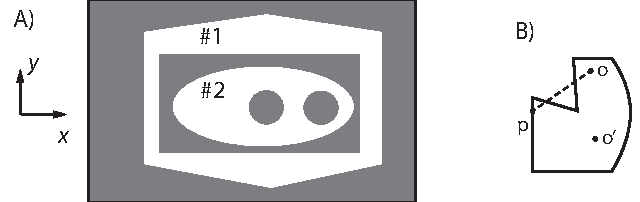
\includegraphics[width=5in]{diffraction-plate.pdf}
  \caption[Example mask wall]{
A) The diffraction plate or mask surface is divided into ``clear'' (white) and
``opaque'' (black) areas. In this example there are two clear sections
labeled \#1 and \#2. B) All wall sections must be star shaped with
respect to the section's origin. In this example, The section is {\em
not} star shaped since a line drawn from the origin point $o$ to the
point $p$ on the boundary intersects the boundary twice in between. In
this case the section can be made star shaped by moving the origin to
$o'$.
  }
  \label{f:diff.plate}
\end{figure}

The \vn{wall} of a \vn{diffraction_plate} or \vn{mask} element
specifies what areas of the
element will transmit or reflect particle and what areas will not. The
areas where there is transmission or reflection are called ``clear''
areas and everything else is called ``opaque''. 

A \vn{wall} is comprised a a ordered list of \vn{sections} as
discussed in \sref{s:wall.section}. Each section of the wall must have
its \vn{type} attribute set to one of:
\begin{example}
  clear
  opaque
\end{example}
A section is called ``clear'' or ``opaque'' depending upon the setting
of its \vn{type} attribute. Do not confuse ``clear section'' with 
``clear area''.

A clear area is defined by one or more consecutive wall sections. The
first section that defines a clear area must be a clear section.  All
the other sections associated with a clear area must be opaque sections.
That is, a clear area starts with a clear section and any preceeding
opaque sections up to the next clear section or the end of the section
list. As a consequence of the above rules, the fist section of the
wall must be a clear section and the number of clear areas is equal to
the number of clear sections.

The default behavior is that a photon will be transmitted if it is
within any clear area. A photon is considered to be within a given
clear area if its $(x,y)$ coordinates put in within the corresponding
clear section but not within any \vn{opaque} section of the clear area.
\vn{Opaque} sections only affect the clear area they are associated
with. See the example below.

Any clear section can be given a \vn{material} and
\vn{thickness}. Available materials are listed in
\sref{s:cryst.list}. A photon transversing a clear area with a defined
material will be attenuated and have a phase shift. Note that
\vn{material} and \vn{thickness} properties are not to be assigned to
\vn{opaque} sections.

To enable \bmad to quickly calculate whether a photon has landed on a
clear or opaque section, All sections, both clear and opaque, must be
``star shaped'' with respect to the $(x_0, y_0)$ origin used by the
section. That is, a line drawn from the section origin to any point on
the section boundary must not pass through any boundary points of the
section in between. This is illustrated in \fig{f:diff.plate}B where
the section is not star shaped since a line drawn from the origin $o$
to the point $p$ on the boundary passes through two boundary points in
between. In this case the section can trivially be made star shaped by
moving the origin to point $o'$. If it is not possible to make a
section star shaped by moving the origin, the section must be divided
into multiple sections.

An example geometry is shown in \fig{f:diff.plate}A.
In the figure, there are two openings labeled \#1, and \#2. A
wall that constructs this geometry is:
\begin{example}
  z_plate: diffraction_plate, wall = \{
    thickness = <real>
    opaque_material = <material_type>
    clear_material = <material_type>
    section = \{           ! Clear area \# 1
      type = clear, 
      v(1) = \{0.04, 0\}, v(2) = \{0.04, 0.022\},
      v(3) = \{0, 0.03\},
    section = \{
      type = opaque,
      v(1) = \{0.032, 0.016\},
    section = \{          ! Clear area \# 2
      type = clear,
      v(1) = \{0, 0, 0.03, 0.013\},
    section = \{
      type = opaque,
      v(1) = \{0, 0, 0.005\},
    section = \{
      type = opaque,
      r0 = (0.02, 0.00),
      v(1) = \{0, 0, 0.005\} \}
\end{example}
Clear area \#1 has a clear section and one opaque section. These
sections rely on the four fold symmetry of the sections so that only
points in the first quadrant need be specified. Clear area \#2 has one
clear section in the shape of an ellipse with two opaque circles. Notice
that the \vn{opaque} section of clear area \#1 does not affect the clear
area \#2 even though it (completely) overlaps clear area \#2.

Sections may overlap and a opaque section does not have to be wholly
within the corresponding clear section. If a photon is within multiple
clear areas then, for the purposes of calculation, it is considered to
be within the first possible clear area in the list.

%-----------------------------------------------------------------
\section{Length Attributes}
\label{s:l}

\index{length of elements}
\index{l|hyperbf}
\index{l_chord|hyperbf}
\index{rbend}
\index{sbend}
The length attributes are
\begin{example}
  l       = <Real>  ! 
  l_chord = <Real>  ! Chord length of a bend. Dependent attribute.
\end{example}
The length \vn{l} is the path length of the reference particle. The
one exception is for an \vn{rbend}, the length \vn{l} set in the
lattice file is the chord length (\sref{s:bend}). internally, \bmad
converts all \vn{rbend}s to \vn{sbend}s and stores the chord length
under the \vn{l_chord} attribute.
Example:
\begin{example}
  b: rbend, l = 0.6   ! For rbends, l will be converted to l_chord
\end{example}

\index{girder}
For a \vn{girder} element the length \vn{l} is a dependent attribute
and is set by \bmad to be the difference in longitudinal position $s$
of the downstream end of the last element supported relative to the
upstream end of the first element. 

\index{wiggler}
For \vn{wiggler}s, the length \vn{l} is not the same as the
path length for a particle with the reference energy starting on the
reference orbit. See~\sref{s:ref}.

\index{patch}
For \vn{patch} elements the \vn{l} length is, by definition, equal to
\vn{z_offset}. For \vn{patch} elements, \vn{l} is a dependent
attribute and will be automatically set to \vn{z_offset} by \bmad.

\index{capillary}
The length of a \vn{capillary} element is a dependent variable and is
given by the value of \vn{s} of the last wall cross-section
(\sref{s:wall.capillary}).

\index{crystal}
The length of a crystal is zero for Bragg diffraction and is a
dependent attribute dependent upon the crystal thickness for Laue
diffraction. See \sref{s:crystal} for more details.

%-----------------------------------------------------------------
\section{Is_on Attribute}
\label{s:is.on}
\index{is_on|hyperbf}

The \vn{is_on} attribute
\begin{example}
  is_on = <Logical>
\end{example}
is used to turn an element off. Turning
an element off essentially converts it into a drift.
Example
\begin{example}
  q1: quad, l = 0.6, k1 = 0.95
  q1[is_on] = False
\end{example}

\index{aperture}
\index{reference orbit}
\index{reference energy}
\vn{is_on} does not affect any apertures that are set. Additionally,
\vn{is_on} does not affect the reference orbit. Therefore, turning 
off an \vn{lcavity} will not affect the reference energy.

The following elements cannot be ``turned off:''
\begin{example}
  beginning_ele
  capillary
  crystal
  drift
  fiducial
  floor_shift
  patch
  group
  null_ele
  overlay
  hybrid
  mirror
  multilayer_mirror
  photon_init
  sample
\end{example}


%-----------------------------------------------------------------
\section{Multipole Attributes: Magnetic and Electric}
\label{s:multip}

Multipole formulas for are given in \sref{s:mag.field} and \sref{s:elec.field}. Note that
the setting of \vn{field_master} (\sref{s:field.master}) will determine if multipoles
are interpreted as normalized or unnormalized.

\index{multipole!knl, tn|hyperbf} 
\index{multipole}
A \vn{multipole} (\sref{s:mult}) element specifies its magnetic
multipole components using an Amplitude (\vn{KnL}) and a tilt
(\vn{Tn})
\begin{example}
  KnL = <Real>
  Tn  = <Real>  ! Default is $pi$/(2n + 2)
\end{example}
Where \vn{n} is an integer in the range from 0 (dipole component)
through 21.  If \vn{Tn} is given without a value, a default of
$pi$/(2n + 2) will be used producing a skew field. Example:
\begin{example}
  m: multipole, k1l = 0.32, t1  ! Skew quadrupole of strength 0.32
\end{example}
Following \vn{MAD}, a non-zero dipole (\vn{K0L} component will affect
the reference orbit (just like a normal dipole will). This is not true
for any other element.

\index{ab_multipole}
\index{multipole!an, bn|hyperbf} 
An \vn{ab_multipole} (\sref{s:ab.m}) specifies magnetic multipoles
using normal (\vn{Bn}) and skew (\vn{An}) components:
\begin{example}
  An = <Real>
  Bn = <Real>
\end{example}
Here \vn{n} ranges from 0 (dipole component) through 21. Example:
\begin{example}
  q1: ab_multipole, b2 = 0.12, a20 = 1e7, field_master = T
\end{example}

\index{r0_mag}\index{scale_multipoles}
Elements like \vn{quadrupoles} and \vn{sextupoles} can have assigned to them both magnetic and
electric multipole fields. In this case, the magnetic fields are specified using the same convention
as the \vn{ab_multipole}.  For such non-multipole elements, the magnetic multipole strength is
scaled by a factor $F \, r_0^{n_\text{ref}} / r_0^n$ (cf.~\Eq{ababf}) where $F$ is the strength of
the element (for example $F$ is $K1 \cdot L$ for a quadrupole), and $r_0$ is the ``measurement
radius'' and is set by the \vn{r0_mag} attribute. The default value of $r_0$.  This behavior may be
turned off by setting the \vn{scale_multipoles} attribute.  Example:
\begin{example}
  q1: quadrupole, b2 = 0.12, a20 = 1e7, scale_multipoles = F
\end{example}
Alternatively, a value of zero (the default) for \vn{r0_mag} is equivalent to setting
\vn{scale_multipoles} to False.

Electric multipoles are specified using normal (\vn{Bn_elec}) and skew
(\vn{An_elec}) components. \begin{example}
  An_elec = <Real>
  Bn_elec = <Real>
\end{example}
Here \vn{n} ranges from 0 (dipole component) through 21. Like the magnetic multipoles, 
a measurement radius \vn{r0_elec} can be used to scale the multipoles as explained in 
\sref{s:elec.field}.
Example:
\begin{example}
  q1: quadrupole, l = 1.2, b2_elec = 1e6, r0_elec = 0.034
\end{example}
See \sref{s:elec.field} for how electric multipoles are defined. Notice that Electric
multipoles are never scalled by the element's field strength as they are with magnetic
multipoles. If the value of \vn{r0_elec} is zero (the default) the multipoles will not
be scalled. 

Unlike magnetic multipoles, there are no factors of the reference momentum nor the element
length in the definition for electric multipoles. That is, electric multipole values
represent the field and not the normalized integrated field. Thus an electric multipole
associated with a zero length element will have no effect on tracking. This being the
case, \bmad does not allow electric multipole values to be specified for \vn{multipole}
and \vn{ab_multipole} elements. Indeed, in the limit of zero element length at constant
integrated electric field strength, the equations of motion are singular since, unlike the
magnetic case, the infinite fringe fields give rise to infinite energy shifts.

\index{multipoles_on}
The magnetic and electric multipole kick can be toggled on or off using the
\vn{multipoles_on} attribute. Example:
\begin{example}
  call, file = 'lattice.bmad'             ! Read in a lattice file
  quadrupole::*[multipoles_on] = False    ! But I want the multipoles off.
  q1[k1] = 0.3                            ! k1 attribute not affected.
\end{example}
\vn{multipoles_on} only effect multipoles specified by \vn{An}, \vn{Bn}, \vn{An_elec}, or
\vn{Bn_elec}. Other multipoles, like the \vn{k2} multipole of a \vn{sextupole}, are not
affected. The exception is \vn{multipole} and \vn{ab_multipole} elements do not have the
\vn{mulipoles_on} attribute. Rather they can be toggles on/off using the \vn{is_on}
attribute.

%-----------------------------------------------------------------
\section{Field Maps}
\label{s:fieldmap}
\index{field maps}

There are two general ways to specify complicated electro-magnetic field configurations
that cannot be simply modeled using multipoles. One way is to use \vn{custom}
fields. Specifying a custom field is done by using custom code and linking this code with
\bmad into a program. That is, custom fields are defined outside of the \bmad software
(\sref{s:integ}).

\index{cylindrical_map}\index{cartesian_map}\index{grid_field}\index{taylor_field}
The other way to specify a complicated field is to use a ``\vn{field map}''. There
are four types of field maps:
\begin{example}
  cartesian_map       ! \sref{s:cart.map}
  cylindrical_map     ! \sref{s:cylind.map}
  grid_field          ! \sref{s:grid.field}
  taylor_field        ! \sref{s:taylor.field}
\end{example}
Essentially, \vn{cylindrical_map} and \vn{cartesian_map} define fields using a set of
functions with user defined coefficients with the functions formulated to obey Maxwell's
equations. The \vn{grid_field} type defines the field on a grid of points and
interpolation is used to evaluate the field inbetween the points. Finally, the
\vn{taylor_field} type defines a set of Taylor maps. Each map defines the field in the
transverse $(x, y)$ plane at constant $z$. Interpolation is used to evaluate the field
in between the planes.

The \vn{cylindrical_map} and \vn{grid_field} types can be used with both RF and DC fields.
The other two types can only be used with DC fields. RF fields may only be used with the following
element classes:
\begin{example}
  e_gun         ! \sref{s:e.gun}
  em_field      ! \sref{s:em.field}
  lcavity       ! \sref{s:lcav}
  rfcavity      ! \sref{s:rfcav}
\end{example}

An element may specify multiple fields of a given type and/or may define multiple fields
of different types. In both these cases, the field in the element is taken to be the sum
of the individual fields. For example:
\begin{example}
  sb: sbend, field_calc = fieldmap, cylindrical_map = \{...\},  cylindrical_map = \{...\}
\end{example}
In this example an element has two \vn{cylindrical_map} fields and the total field is the
sum of the fields of each one. Separating fields like this can be useful, for example, to
decouple the specification of electric from magnetic fields, or to decouple the
specification of AC and DC fields.

fields may stored in a \vn{binary} format (\sref{s:binary.form}). For example:
\begin{example}
  qq: quadrupole, grid_field = call::my_grid.bin, ...
\end{example}

The field of one element can overlap onto other elements. This is
explained in Sec.~\sref{s:overlap}.

Field maps are used with integration type tracking methods (\sref{s:integ}).
It is important to note that field maps are {\em ignored} by \vn{bmad_standard}
tracking. Field maps may extend longitudinally beyound the ends of an element
(\sref{s:overlap}).

In a lattice file, once a field map is defined for an element, components of the field map
may be redefined using the notation
\begin{example}
  ele_name[field_map_name(index)%component_name] = value
\end{example}
where \vn{ele_name} is the name of the element, \vn{field_map_name} is the name of the
type of field map, \vn{index} is the index of the field map which is ``1'' for the first
field map defined for an element, etc., \vn{component_name} is the name of the component,
and \vn{value} is the value to set to. Example:
\begin{example}
  qq, quadrupole, grid_field = \{field_scale = 0.5, ...\}, ...
  qq[grid_field(1)%field_scale] = 0.7  ! Change field_scale value
\end{example}

%-----------------------------------------------------------------
\subsection{Field Map Common attributes}
\label{s:fieldmap.com}

\begin{figure}[tb]
  \centering
  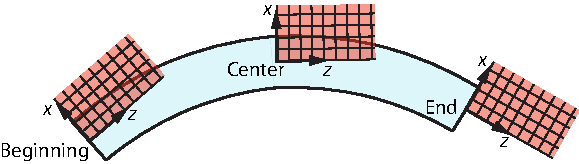
\includegraphics{bend-grid-coords.pdf}
  \caption[\vn{Field map} coordinates when used with a bend element.]{
When used with a bend element, by default, field map coordinates will be Cartesian and not
curved like the reference orbit. The orientation of the field map coordinates is
determined by the setting of \vn{ele_anchor_pt}. To use curvilinear coordinates instead,
\vn{curved_ref_frame} must be set to \vn{True} [Available in \vn{grid_field} and
\vn{taylor_field} only].}
  \label{f:bend.grid}
\end{figure}

This section explains some of the attributes that are common to the \vn{field map}
types. Not all attributes are used in all field map types. See the documentation on the
individual types for a list of the attributes pertainent to that type.

\index{field_type}
\index{field_scale}\index{master_parameter}
  \begin{description}
  \item[curved_ref_frame] \Newline
For bends, the coordinates of the field are, by default, Cartesian and do not follow the
curved bend coordinates. The orientation of the field map coordinates with respect to the
bend is determined by the placement of the anchor point (specified by \vn{ele_anchor_pt})
as shown in \fig{f:bend.grid}. In this case, when tracking a particle, \bmad will convert
particle coordinates (which are expressed in the bend's curvilinear coordinate system
defined by the reference orbit) to the Cartesian coordinates of the field map and will
rotate the computed field from the field map coordinates back to the particle coordinates.

For \vn{grid_field} and \vn{taylor_field} types only, this default behavior can be changed by
setting the \vn{curved_ref_frame} component of the field map to \vn{True}. In this case,
the field grid coordinates will follow curved bend coordinates.  The \vn{curved_ref_frame}
parameter is only pertinent for bend elements (\vn{sbend}s, \vn{rbend}s).  The setting of
\vn{curved_ref_frame} is ignored for non-bend elements.
  \item[ele_anchor_pt] \Newline
The \vn{ele_anchor_pt}, along with \vn{r0}, determines the origin of the field with
respect to the lattice element. Possible settings are:
\begin{example}
  beginning   ! Beginning of element (default).
  center      ! Center of element.
  end         ! Exit end of element.
\end{example}
Example:
\begin{example}
  rfc0: rfcavity, taylor_field = \{ele_anchor_pt = center, ...\}, ...
\end{example}
  \item[field_type] \Newline
The \vn{field_type} attribute sets the type of field described. Possible settings for
\vn{field_type} are:
\begin{example}
  electric      ! Pure electric field. For DC fields only.
  magnetic      ! Pure magnetic field. For DC fields only.
  mixed         ! Mixed EM fields. For AC fields and DC \vn{grid_field}.
\end{example}
Example:
\begin{example}
  bb: sbend, cartesian_map = \{field_type = electric, ...\}, ...
\end{example}
The \vn{cylindrical_map} type does not have a \vn{field_type} since it has explicit arrays
for the electric and magnetic fields.
  \item[field_scale] \Newline
The \vn{field_scale} attribute is used to scale the overall field magnitude. The default
value is 1. A value of -1 will reverse the field. If the \vn{master_parameter} is
defained, it is multiplied with the \vn{field_scale} to give the overall scale.
Example:
\begin{example}
  qq, quadrupole, grid_field = \{field_scale = 0.5, ...\}, ...
\end{example}
  \item[harmonic] \Newline
The \vn{harmonic} attibute, along with \vn{rf_frequency} element attribute, sets the
oscillation frequency of the field map. The \vn{harmonic} attribute is only used with
\vn{cylindrical_map} and \vn{grid_field} types. The default value of \vn{harmonic} is 0.
The \vn{harmonic} number needs to be 0 for DC fields. Example:
\begin{example}
  lc1: lcavity, rf_frequency = 500e6, grid_field = \{harmonic = 2, ...\}, ...
\end{example}
Notice that \vn{rf_frequency} is set outside of any field map and is common to all field maps.
  \item[master_parameter] \Newline
The \vn{master_parameter} defines a ``master'' element attribute for scaling the field. Example:
\begin{example}
  qq: quadrupole, taylor_field = \{master_parameter = 'K1', ...\}, k1 = ...
\end{example}
This example defines the \vn{master_parameter} for the \vn{taylor_field} to be the
quadrupole strength \vn{k1}. By using the same master parameter for a set of field map
instances within a given lattice element, the sum field of the set can be controled by a
single attribute. The \vn{master_parameter} must be set to a valid element attribute. If
the name is blank (""), no master parameter is used. The \vn{master_parameter}, if
defined, is multiplied with the \vn{field_scale} to give the value used to scale the
fields. The default \vn{master_parameter} is blank ("") except for \vn{wiggler} elements
where, for historical reasons, the default is \vn{polarity}.
  \item[phi0_fieldmap] \Newline
For AC fields, \vn{phi0_fieldmap} is the phase of the field map field relative to the
fundamental mode. [Note: Documentation on the phase of the fundamental mode is given in
the appropriate section for the type of element under consideration (\vn{e_gun},
\vn{lcavity}, etc.).] The phase \vn{phi0_fieldmap} is relative to the fundamental
frequency and not the frequency of the field map mode. That is, the ``zero crossing'' time
of the field map is shifted by \vn{phi0_fieldmap}/$f_0$ where $f_0$ is the fundamental
mode frequency.
  \item[r0] \Newline
The \vn{r0} attribute is the $(x0, y0, z0)$ vector specifying the offset of the origin point
that defines the field relative to the \vn{anchor} point defined by \vn{ele_anchor_pt}.
The origin position of the field (\vn{r_origin}) is determined by 
\begin{example}
  r_origin = r0 + r_anchor
\end{example}
where \vn{r_anchor} is determined by the setting of \vn{ele_anchor_pt}. In the reference
coordinates (\sref{s:ref}) with respect to the element \vn{r_anchor} is:
\begin{example}
  ele_anchor_pt       r_anchor
  -------------       ---------
  beginning           (0, 0, 0)      ! Default
  center              (0, 0, L/2)
  end                 (0, 0, L)
\end{example}
with \vn{L} being the length of the element. 

Example:
\begin{example}
  rfc0: rfcavity, taylor_field = \{r0 = (-0.23, ...), ...\}, ...
\end{example}
  \end{description}

%-----------------------------------------------------------------
\subsection{Cartesian_Map Field Map}
\label{s:cart.map}
\index{cartesian_map}

The \vn{cartesian_map} field map is only used for DC fields. Each term of a
\vn{cartesian_map} is a solution of Laplace's equation in cartesian coordinates.
as described in Sec.~\sref{s:cart.map.phys}. 

The lattice file syntax for the \vn{cartesian_map} type is:
\begin{example}
  cartesian_map = \{
    field_type       = <String>,           ! Type of field: Default = Magnetic.
    field_scale      = <Real>,             ! Scale factor for the E & B fields.
    master_parameter = <Name>,             ! Master scaling parameter for E & B fields.
    ele_anchor_pt    = <Position>,         ! Anchor position: Beginning (default), Center, or End.
    r0               = (<x0>, <y0>, <z0>), ! Anchor offset. Default is 0.
    term = \{<A>, <k_x>, <k_y>, <k_z>, <x_0>, <y_0>, <phi_z>, <family>\}, 
    term = \{....\}  \}
\end{example}
The possible settings of \vn{<family>} are explained in Sec.~\sref{s:cart.map.phys}.
Example:
\begin{example}
  q01: quadrupole, l = 0.6, field_calc = fieldmap,
        cartesian_map = \{
          term = \{0.03, 3.00, 4.00, 5.00, 0, 0, 0.63, y\},
          term = \{...\}, ...    \}
\end{example}

See Sec.~\sref{s:fieldmap.com} for an explanation of the attributes that are common with
other field map types. 

To use with PTC dependent tracking methods (\sref{s:integ}) there are a number of
restrictions: 
  \begin{itemize}
  \item
There can be only one \vn{cartesian_map} field map and there cannot be any other field
maps of any kind.
  \item 
\vn{cartesian_map} may not be used with a bend.
  \item
Only magnetic fields may be used. 
  \item
The transverse terms in \vn{r0} must be zero.
  \end{itemize}

%-----------------------------------------------------------------
\subsection{Cylindrical_Map Field Map}
\label{s:cylind.map}
\index{ccylindrical map}

The \vn{cylindrical_map} field map is used for both DC and AC fields. Each term of a
\vn{cylindrical_map} is a solution of Laplace's equation in cylindrical coordinates.
as described in Sec.~\sref{s:cylind.map.phys}. 

The lattice file syntax for the \vn{cylindrical_map} type is:
\begin{example}
  cylindrical_map = \{
    field_scale      = <Real>,             ! Scale factor for the E & B fields.
    master_parameter = <Name>,             ! Master scaling parameter for E & B fields.
    ele_anchor_pt    = <Position>,         ! Anchor position: Beginning (default), Center, or End.
    m                = <Integer>,          ! Azimuthal mode number
    harmonic         = <Integer>,          ! RF frequency harmonic number 
    phi0_fieldmap    = <Real>,             ! Phase of oscillations.
    theta0_azimuth   = <Real>,             ! Azimuthal orientation.
    r0               = (<x0>, <y0>, <z0>), ! Anchor offset. Default is 0.
    dz        = <Real>,                    ! Distance between sampled field points.
    e_coef_re = (<Real>, <Real>, ....),    ! Real part of E.
    e_coef_im = (<Real>, <Real>, ....),    ! Imaginary part of E.
    b_coef_re = (<Real>, <Real>, ....),    ! Real part of B.
    b_coef_im = (<Real>, <Real>, ....),    ! Imaginary part of B.
  \}
\end{example}
See Sec.~\sref{s:fieldmap.com} for an explanation of the attributes that are common with
other field map types.

For DC fields, the \vn{e} coefficients specify the electric fields and the \vn{b} coefficients
specify the magnetic fields. For AC fields, the \vn{e} coefficients specify modes that have finite
longitudinal fields while the modes associated with the \vn{b} coefficients do not.

To specify the RF frequency, specify the \vn{rf_frequency} {\em element} attribute along with
the \vn{harmonic} attribute. See the discussion of the \vn{harmonic} attribute in 
Sec.~\sref{s:fieldmap.com}.

The basic equations used for the \vn{cylindrical_map} decomposition of the fields are given in
Section~\sref{s:cylind.map.phys}. A lattice element may have multiple \vn{cylindriacl_map}
components with each \vn{cylindrical_map} being associated with a particular azimuthal mode $m$.

\vn{e_re} and \vn{e_im} give the real an imaginary part of $e$ and \vn{b_re} and \vn{b_im} give the
real and imaginary part of $b$. All of these vectors must be present and have the same length. The
exception is with an $m = 0$ mode either the $e$ or $b$ arrays can be omitted and will default to
zero. The number of terms $N$ for the $e$ or $b$ vectors must be a power of $2$ and all modes must
have the same number of terms. The $n$\Th element in the $e$ or $b$ arrays, with $n$ running from 0
to $N-1$, is associated with a wavelength $k_n$
\begin{equation}
  k_n = \begin{cases}
    \frac{2 \, \pi \, n}{N \, dz} & 0 \le n < \frac{N}{2} \\
    \frac{2 \, \pi \, (n-N)}{N \, dz} & \frac{N}{2} \le n \le N - 1
  \end{cases}
\end{equation}
This convention produces less high frequency components then the convention of using $k_n = 2 \, \pi
\, n / N dz$.

The longitudinal length of the field is
\begin{equation}
  L_{\text{field}} = \frac{N - 1}{dz}
\end{equation}
this may be different from the length \vn{l} specified for the
element.

Example:
\begin{example}
  m1: lcavity, rf_frequency = 1e6, voltage = 2e6, cylindrical_map = \{
    m = 2,                   harmonic = 3,
    r0 = (0, 0, 0.001),      dz = 0.1,
    theta0_azimuth = 0.3,    field_scale = 0.7,
    ele_anchor_pt = center,  master_parameter = voltage,
    e_coef_re = (...),       e_coef_im = (...),
    b_coef_re = (...),       b_coef_im = (...)\}, field_calc = fieldmap
\end{example}

Note: When using PTC based tracking (\sref{c:methods}), the following restrictions apply:
\begin{Itemize}
\item
The fields must be DC.
\item
all the \vn{e_coef} and \vn{b_coef} arrays must have the same length.
\item
\vn{r0(1)} and \vn{r0(2)} (the transverse offsets) must be zero.
\item
The element containing the map cannot be an \vn{sbend} or \vn{rbend}.
\item
May not be combined with other field map types.
\end{Itemize}

%-----------------------------------------------------------------
\subsection{Grid_Field Field Map}
\label{s:grid.field}
\index{grid field}

A \vn{grid_field} is grid of field points specified using the syntax:
\begin{example}
  grid_field = \{ 
    geometry         = <String>,    ! Geometry of the grid.
    field_type       = <String>,    ! Type of field: Default = Mixed.
    field_scale      = <Real>,      ! Scale factor for the E & B fields.
    phi0_fieldmap    = <Real>,      ! Phase of oscillations.
    harmonic         = <Integer>,   ! RF frequency harmonic number 
    master_parameter = <Name>,      ! Master scaling parameter for E & B fields.
    curved_ref_frame = <Logical>,   ! Use a curved reference frame with bends?
    r0   = (...),                   ! Grid origin. Syntax is \vn{geometry} dependent.
    dr   = (...),                   ! Grid spacing. Syntax is \vn{geometry} dependent.
    ele_anchor_pt = <Position>      ! BEGINNING, CENTER, or END
    pt(<Integer>, \dots) = ( \ldots ), ! Field points. Syntax is \vn{geometry} dependent.
    \ldots \} \} \}
\end{example}
See Sec.~\sref{s:fieldmap.com} for an explanation of the attributes that are common with
other field map types.

To specify the RF frequency, specify the \vn{rf_frequency} {\em element} attribute along with
the \vn{harmonic} attribute. See the discussion of the \vn{harmonic} attribute in 
Sec.~\sref{s:fieldmap.com}.

For \vn{field_type} set to \vn{electric} or \vn{magnetic}, the field is DC. That is, For
\vn{field_type} set to \vn{electric} or \vn{magnetic}, the value of \vn{harmonic} must be
0. For \vn{field_type} set to \vn{mixed}, the field may be DC or AC. In this case, the
individual field components are complex.  the syntax for specifying a complex number is:
\begin{example}
  (<Re>, <Im>)
\end{example}
where \vn{<Re>} and \vn{<Im>} are the real and imaginary parts of the
component. Example:
\begin{example}
  pt(0, 0, -7) = ((0.34, -4.3), (2.37, 9.34), ...)  ! Complex field
  pt(0, 0, -7) = (0.12, -0.33, ...)                 ! Imaginary components are zero
\end{example}

The \vn{geometry} switch sets the type of the grid and must come before
any \vn{pt} is given. The possible settings of \vn{geometry} are:
\begin{example} 
  rotationally_symmetric_rz
  xyz
\end{example}

The \vn{rotationally_symmetric_rz} setting for \vn{geometry} is for fields
that are rotationally symmetric around the $z$ axis. The format for
this type of \vn{grid_field} is
\begin{example}
  grid_field = \{ 
    geometry = rotationally_symmetric_rz,
    r0   = (<x0>, <y0>, <z0>),  ! Grid origin 
    dr   = (<dr>, <dz>),        ! Grid spacing
    pt(<ir>, <iz>) = (<E_r>, <E_phi>, <E_z>) ! For field_type = Electric
    pt(<ir>, <iz>) = (<B_r>, <B_phi>, <B_z>) ! For field_type = Magnetic
    pt(<ir>, <iz>) = (<E_r>, <E_phi>, <E_z>, <B_r>, <B_phi>, <B_z>)
                                             ! For field_type = Mixed.
    \ldots \} 
\end{example}
where \vn{<iz>} can be negative but \vn{<ir>} must be non-negative.  

The \vn{xyz} setting for \vn{geometry} can be used for all rectangular field grids. The
format for this type of \vn{grid_field} is
\begin{example}
  grid_field = \{ 
    geometry = xyz,
    r0   = (<x0>, <y0>, <z0>),    ! Grid origin 
    dr   = (<dx>, <dy>, <dz>),    ! Grid spacing
    pt(<ix>, <iy>, <iz>) = (<E_x>, <E_y>, <E_z>),  ! For field_type = Electric
    pt(<ix>, <iy>, <iz>) = (<B_x>, <B_y>, <B_z>),  ! For field_type = Magnetic
    pt(<ix>, <iy>, <iz>) = (<E_x>, <E_y>, <E_z>, <B_x>, <B_y>, <B_z>), 
                                                   ! For field_type = Mixed.
    \ldots \}
\end{example}
where \vn{<ix>}, \vn{<iy>}, and \vn{<iz>} can be negative.

[For clarity sake, the following discusses the \vn{xyz} case. Extension to other cases is
straight forward.]  There is no restriction on the bounds of the indexes \vn{(ix, iy, iz)}
of the \vn{pt(ix, iy, iz)} array. A point $(ix, iy, iz)$ corresponds in space to the point
$(x, y, z)$:
\begin{example}
  (x, y, z) = dr * (ix, iy, iz) + r0 + r_anchor
\end{example}
where \vn{z} is measured from the beginning of the element and
\vn{r_anchor} is determined by the setting of \vn{ele_anchor_pt}:
\begin{example}
  ele_anchor_pt       r_anchor
  -------------       ---------
  beginning           (0, 0, 0)      ! Default
  center              (0, 0, L/2)
  end                 (0, 0, L)
\end{example}
with \vn{L} being the length of the element. 

Example:
\begin{example}
  apex: e_gun, l = 0.23, field_calc = fieldmap, rf_frequency = 187e6, 
                                  grid_field = call::apex_gun_grid.bmad
\end{example}
with the file \vn{apex_gun_grid.bmad} being:
\begin{example}
  \{
    geometry = rotationally_symmetric_rz,
    harmonic = 1,
    master_parameter = voltage,
    r0 = (0, 0),
    dr = (0.001, 0.001),
    pt(0,0) = ( (0, 0), (0, 0), (1, 0),  (0, 0), (0, 0), (0, 0)),
    pt(0,1) = ( (0, 0), (0, 0), (0.99, 0),  (0, 0), (0, 0), (0, 0)),
    ... \}
\end{example}

It is considered an error if the field of the grid is evaluated for a point that is transversely
outside of the grid. That is, a grid must extend transversely to the aperture or at least beyound
the trajectory of any particle. [Actually, to prevent problems when the aperture is set at the grid
boundary, if the distance between the particle and the grid boundary is within 1/2 of the spacing
between grid points, no error is generated and the field will calcuated using extrapolation.] On the
other hand, it is acceptable to evaluate the grid field at a point that is longitudinally outside of
the grid. In this case, the field is assumed to go to zero. This is done by effectively adding to
the grid two planes of zero field longitudinally to either side of the grid. So a particle traveling
ouside of the grid longitudinally will see the field drop to zero within one longitudinal grid
spacing length.

%-----------------------------------------------------------------
\subsection{Taylor_Field Field Map}
\label{s:taylor.field}
\index{taylor field}

The \vn{taylor_field} field map is only used for DC fields. A \vn{taylor_field} is comprised
of a set of two dimensional Taylor maps.  

The syntax for describing a \vn{taylor_field} is:
\begin{example}
  taylor_field = \{
    field_type       = <String>,           ! Type of field: Default = Magnetic.
    field_scale      = <Real>,             ! Scale factor for the E & B fields.
    master_parameter = <Name>,             ! Master scaling parameter for E & B fields.
    curved_ref_frame   = <Logical>,        ! Use curved coords with bends?
    canonical_tracking = <logical>         ! Use (px, py) instead of (x', y') when tracking?
    ele_anchor_pt    = <Position>,         ! Anchor position: Beginning (default), Center, or End.
    r0               = (<x0>, <y0>, <z0>), ! Anchor offset. Default is 0.
    dz               = <Real>,             ! Distance between sampled field points.
    plane(<i>) = \{<term1>, <term2>, <term3>, ....\}, ! Taylor map at constant z.
    plane(<j>) = \{....\}  \}
\end{example}
See Sec.~\sref{s:fieldmap.com} for an explanation of the attributes that are common with
other field map types.

Each \vn{plane(<i>)} component specifies a Taylor map at constant z
(\sref{s:taylor.field.phys}). The index \vn{<i>} for the different planes must be in
consecutive order. The plane with <i> = 0 corresponds to the $z = 0$ origin. There is no
restriction for the starting \vn{<i>} index of the first plane. That is, there does not
have to be a plane with index \vn{<i>} = 0 (in this case, the origin needs to be outside
of the element).

The individual Taylor series terms follow the same syntax as the Taylor terms in a
\vn{taylor} element (\sref{s:taylor}):
\begin{example}
  \{<out>: <coef>, <e1> <e2>\}           ! EM Taylor term. First form.
  \{<out>: <coef> | <n1> <n2> ...\}      ! EM Taylor term. Second form.
\end{example}
except that 1) \vn{<out>} must be one of
\begin{example}
  Bx, By, or Bz
\end{example}
2) there are only two exponents \vn{<e1>} and \vn{<e2>}
corresponding to \vn{x}, and \vn{y} respectively for the first form,  and 3) the integers
\vn{<n1>}, \vn{<n2>}, etc., are restricted to being 1 or 2.

To use with PTC dependent tracking methods (\sref{s:integ}) there are a number of
restrictions: 
  \begin{itemize}
  \item
There can be only one \vn{taylor_field} field map and there cannot be any other field
maps of any kind.
  \item 
The number of planes must be odd. If you want to be able to track with PTC to the center
of the element, the number of planes must be of the form $4 \, n + 1$ where $n$ is an
integer.
  \item
Only magnetic fields may be used.
  \item
The plane locations must be symmetric with respect to the center of the element. That is,
the first plane and the last plane must be equidistant from the element center.
  \item
The element may not be superimposed upon (\sref{s:super}). [PTC tracks from plane to plane
so there is no good way to cut an element at an arbitrary position.]
  \item
In a bend with \vn{curved_ref_frame} = False, The setting of \vn{ele_anchor_pt} must be
\vn{center}.
  \end{itemize}
If the edges of the \vn{taylor_field}, which are defined by the first and last planes, is
different than the edges of the element, \bmad and PTC will do tracking differently. With
\bmad, the tracking will start at one edge of the element and will end at the other
end. That is, \bmad will ignore the field outside of the element (but this can be modified
using field overlap (\sref{s:overlap})). PTC, on the other hand, will start at an element
end and then track from the element end backwards to the first plane like in a drift. It
will then track to the ending plane and finally track backwards from the ending plane to
the ending element edge line in a drift. That is, PTC does not ignore the field outside of
the element.

When using PTC based tracking (\sref{c:methods}), the \vn{canonical_tracking} parameter
can be used to select whether the transverse phase space coordinates used in tracking is
the canonical $(x, p_x, y, p_y)$ (\sref{s:phase.space}) coordinates or the non-canonical
$(x, x', y, y')$ coordinates. The default is \vn{False}. The difference comes at the edges
of element if the field is not zero. With canonical coordinates, there is a kick at the
edge while with the non-canonical there is not. What is best depends upon the problem. For
example, with a solenoid magnet where the field is constant right up to the edge,
canonical tracking will be needed since the edge kick is significant. However, the edge
kick is not well defined (that is, certain assumptions are built into the edge kick
calculation. For example, with a solenoid, cylindrical symmetry is generally
assumed). Thus for some arbitrary field, the assumptions used by PTC may by incorrect for
the problem at hand. Thus in many cases, especially for single pass machines, the
non-canonical tracking is a better choice.

Example:
\begin{example}
  t1: sbend, k1 = 2, taylor_field = \{
    field_type = electric,   ele_anchor_pt = end, 
    dz = 1.2,                r0 = (0, 0, 2.0),
    field_scale = 1.3,       curved_ref_frame = False,
    master_parameter = k1,
    plane(-2) = \{\{Bx: 0.3| 1\}, \{Bx: 1.3, 1 2\}, \{By: 0.7, 3 1\}, ...\},
    plane(-1) = \{\{Bx: 0.6|\}, \{By: 0.4|112\}, \{By: 0.7, 4 0\}, ...\}, 
    ...  \}, field_calc = fieldmap
\end{example}

%-----------------------------------------------------------------
\section{RF Couplers}
\label{s:rf.coupler}

\index{lcavity}\index{rfcavity}
\index{coupler_at}\index{coupler_strength}
\index{coupler_angle}\index{coupler_phase}
For \vn{lcavity} and \vn{rfcavity} elements, the attributes that
characterize the dipole transverse kick due to a coupler port are:
\begin{example}
  coupler_at       = <Switch> ! What end the coupler is at
  coupler_strength = <Real>   ! Normalized strength
  coupler_angle    = <Real>   ! Polarization angle (rad/2\(\pi\))
  coupler_phase    = <Real>   ! Phase angle with respect to the RF (rad/2\(\pi\))
\end{example}
The possible \vn{coupler_at} settings are:
\begin{example}
  entrance_end
  exit_end  ! default
  both_ends
\end{example}
The kick due to the coupler is
\begin{example}
  dP_x = amp * cos(phase) * cos(angle) 
  dP_y = amp * cos(phase) * sin(angle)
  dE   = amp * (cos(angle) * x + sin(angle) * y) * sin(phase) * twopi * rf_frequency / c_light 
\end{example}
where \vn{dP_x} and \vn{dP_y} are the transverse momentum kicks, \vn{dE} is an energy kick, and
\begin{example}
  amp   = gradient * coupler_strength 
  phase = twopi * (phase_particle + phase_ref + coupler_phase)         ! For lcavity \sref{s:lcav}
        = pi/2 + twopi * (phase_particle - phase_ref + coupler_phase)  ! For rfcavity \sref{s:lcav}
  angle = twopi * coupler_angle
\end{example}
The energy kick is needed to keep things symplectic. 

Example:
\begin{example}
  rf1: lcav, l = 4.5, gradient = 1.2e6, coupler_at = both_ends,
                                                  coupler_strength = 0.037
\end{example}

%-----------------------------------------------------------------
\section{Field Extending Beyond Element Boundary}
\label{s:overlap}

\index{field_overlaps} 
The \vn{field_overlaps} element attribute can be used to indicate that the electric or
magnetic fields of one element overlap another element. The syntax is:
\begin{example}
  <overlapping_ele>: ... field_overlaps = \{<overlapped_ele1>, <overlapped_ele2>, ...\}
\end{example}
The \{\} braces are optional if there is only one overlapped element.

Example:
\begin{example}
  b1: sbend, l = 2.3, field_overlaps = \{q1, s2\}, ...
  inj_line: line = (..., s2, b1, mark3, q1, ...)
\end{example}
In this example, the field of element \vn{b1} extends beyond the ends of \vn{b1} and
overlaps elements \vn{q1} and \vn{s2}. There is no limit to the number of elements that
are overlapped by any given element and overlapped elements do not have to be next to the
overlapping element in the line. If there are multiple elements whose name matches the
name of a overlapped element, the element closest to the overlapping element is
chosen. Thus in the above example, if there are multiple elements named \vn{q1}, the
closest \vn{q1} to \vn{b1} is designated as the overlapped element.

There can be multipole \vn{field_overlaps = ...} constructs for an overlapping element.
Thus the following is equivalent to the above example:
\begin{example}
  b1: sbend, l = 2.3, field_overlaps = q1, field_overlaps = s2
\end{example}

Note: When the field overlaps elements that are superimposed (\sref{s:super}), the overlapped 
elements must be the \vn{super_lord} elements and never the slaved elements.

The field, when \vn{field_calc} (\sref{s:integ}) is set to \vn{bmad_standard}, never extends beyond the
element boundary and so a \vn{bmad_standard} field will never overlap another element.

%-----------------------------------------------------------------
\section{Automatic Scaling of Accelerating Fields}
\label{s:autoscale}
\index{automatic field scaling|hyperbf}

\index{e_gun}\index{em_field}\index{lcavity}\index{rfcavity}
Elements that have accelerating fields are:
\begin{example}
  e_gun       ! \sref{s:e.gun}
  em_field    ! \sref{s:em.field}
  lcavity     ! \sref{s:lcav}
  rfcavity    ! \sref{s:rfcav}
\end{example}
[Notice that \vn{rfcavity} elements by definition, have a constant reference energy while
with all the other elements the entrance end reference energy will, in general, be
different from the exit end reference energy.]

The problem that arises with accelerating fields is how to set the overall amplitude (and
phase if the fields are oscillating) of the field so that a particle, starting on the
reference orbit and starting with the reference energy, has the desired energy gain at the
exit end of the element where the ``desired'' is set by the \vn{voltage} or \vn{gradient}
attribute of the element.

The scaling problem is not present when \vn{bmad_standard} tracking (\sref{s:tkm}) is used
since \vn{bmad_standard} tracking uses an integrated formula that is designed to give the
proper acceleration. Rather it is a problem for Runge-Kutta and other methods integration
methods.

The problem becomes even more complicated at non-ultra relativistic energies where the
particle velocity is not a constant. In this case, the proper amplitude and/or phase
settings will depend upon what the incoming energy of the reference particle is.

To help with the scaling problem, \bmad has the capability to automatically
scale an accelerating field's amplitude and/or phase. The two
lattice element parameters that turn on/off auto scaling are (\sref{s:param}):
\begin{example}
  autoscale_phase      = <Logical>  ! Automatic phase scaling.
  autoscale_amplitude  = <Logical>  ! Automatic amplitude scaling.
\end{example}
The default value is True for both parameters. Example:
\begin{example}
  rf2: rfcavity, autoscale_phase = F
\end{example}

Scaling takes place during program execution when a lattice is initially created (that is,
when the lattice file is parsed) and when parameters in the lattice that would change the
scaling are varied.  The element parameters varied wen autoscaling is done are:
\begin{example}
  field_autoscale       ! Amplitude scale
  phi0_autoscale        ! phase scale
\end{example}
If no autoscaling is done, the default setting of \vn{field_autoscale} is 1 and the
default setting of \vn{phi0_autoscale} is 0.

\vn{field_autoscale} and \vn{phi0_autoscale} are ignored when \vn{bmad_standard} tracking
is done.

%-----------------------------------------------------------------
\section{Wakefields}
\label{s:wakes}

Wake fields can be specified for many elements.  The attributes that characterize the
wakes are:
\index{sr_wake_file}\index{lr_wake_file}\index{lr_freq_spread}
\begin{example}
  sr_wake_file     = <String>   ! Short range wake field definition file. (\sref{s:sr.wake.file})
  lr_wake_file     = <String>   ! Long range wake field definition file. (\sref{s:lr.wake.file})
  lr_freq_spread   = <Real>     ! RMS fractional frequency spread of the LR wake fields.
  lr_self_wake_on  = <Logical>  ! Apply longitudinal long range self-wake? Default = True.
\end{example}

The \vn{lr_freq_spread} attribute is used to randomly spread out the long range mode
frequencies among different cavities. The spread is Gaussian in shape with an RMS of
\vn{lr_freq_spread} * $F$ where $F$ is the frequency of a mode.

The \vn{lr_self_wake_on} attribute can be used to turn off the longitudinal long-range
self-wake which is the longitudinal kick on the particles of a bunch due to the wake
generated by these same particles. [The transverse self wake is always zero.] The default
setting of \vn{lr_self_wake_on} is \vn{True}. Turning off the self-wake, for example,
can be done to avoid double counting if both long-range and short-range wakes are defined.

Example:
\begin{example}
  abc: lcavity, lr_wake_file = 'lr.wake', lr_freq_spread = 0.0023, lr_self_wake_on = F
\end{example}

The formulas used to compute the wake field are given in \sref{s:wake.fields}. \bmad has
two modes for tracking particles. One mode tracks individual particles one at a time. The
other mode tracks bunches of particles. Which mode is used for a given program is decided
by the program. The wake field is ignored when tracking individual particles and only used
when tracking bunches.

%-----------------------------------------------------------------
\subsection{Short-Range Wakes}
\label{s:sr.wake.file}

\index{wakes!short-range}
The input file name for the short--range wake fields is specified
using the \vn{sr_wake_file} attribute. The file gives both monopole
longitudinal and dipole transverse wakes. An example input file is:
\begin{example}
  ! Pseudo Wake modes:
  !                      Amp       Damp          K      Phase  Polar-    Transverse_
  ! Longitudinal:      [V/C/m]     [1/m]      [1/m]     [rad]  ization   Dependence
  ! Transverse:      [V/C/m^2]     [1/m]      [1/m]     [rad]  

  &short_range_modes
    longitudinal(1) = 3.23e14     1.23e3     3.62e3     0.123
    longitudinal(2) = 6.95e13     5.02e2     1.90e3    -1.503
    .. etc ..
    transverse(1) =   4.23e14     2.23e3     5.62e3     0.789    X  linear_trailing
    transverse(2) =   8.40e13     5.94e2     1.92e3     1.455
     .. etc ..
    z_max = 1.3e-3
  /
\end{example}
Wakes are specified via a set of ``pseudo'' modes
(\sref{s:wake.short}). The magnitude of \vn{z_max} should be set to
the maximum $z$ value at which the pseudo mode fit is valid. \bmad
will check the distance between particles does not exceed \vn{z_max}.
If it does, \bmad will report an error.

\index{none}\index{x_axis}\index{y_axis}
The \vn{polarization} parameter is used to specify the wake
polarization. Possible settings for this parameter are:
\begin{example}
  none    ! Default
  x_axis  
  y_axis 
\end{example}
The \vn{polarization} name may be abbreviated.  For example, if the
\vn{polarization} is set to \vn{x_axis}, there is no vertical kick
from the pseudo mode.

\index{none}\index{linear_leading}\index{linear_trailing}
The \vn{transverse_dependence} parameter sets whether the wake kick
is linear in the offset of the leading or trailing particle or is
independent of the transverse offset.
Possible settings of this parameter are:
\begin{example}
  none              ! Default for longitudinal modes
  linear_leading    ! Default for transverse modes
  linear_trailing
\end{example}
The \vn{transverse_dependence} parameter may be abbreviated. Note: Due
to the way the wake file is parsed, if \vn{transverse_dependence} is
specified for a particular mode, \vn{polarization} must also be
specified.

For \vn{longitudinal} modes: If the \vn{transverse_dependence} is
\vn{none} (the default), then the \vn{polarization} must also be
\vn{none} (other combinations do not make sense). If the
\vn{transverse_dependence} is \emph{not} \vn{none} for a
\vn{longitudinal} mode, then the \vn{polarization} must be set
to \vn{x_axis} or \vn{y_axis}. 

Note: In a beam chamber with circular symmetry, the linear terms in
the \vn{longitudinal} wake are zero and the transverse wake has
no terms independent of the transverse offsets nor terms that
depend upon the trailing particle offset.

%-----------------------------------------------------------------
\subsection{Long-Range Wakes}
\label{s:lr.wake.file}

Equations for long-range wakes is given in \Sref{s:wake.long}.

The input file name for the long--range wake fields is specified using
the \vn{lr_wake_file} attribute. The file gives the wake modes by
specifying the frequency (in Hz), R/Q (in $\Omega$/meter$^{2m}$), Q,
and m (order number), and optionally the polarization angle (in
radians/2pi) for each cavity mode. The input uses Fortran90 namelist
syntax: The data begins with the string \vn{\&long_range_modes} and
ends with a slash \vn{/}. Everything outside this is ignored. Each
mode is labeled \vn{lr(i)} where \vn{i} is the mode index. An example
input file is:
\begin{example}
              Freq      R/Q      Q    m   Polar   b_sin  b_cos a_sin  a_cos  t_ref 
                      [Ohm/               Angle 
              [Hz]     m^(2m)]           [Rad/2pi]
  &long_range_modes
    lr(1) = 1.650e9    0.76    7.0e4  1    "unpol"
    lr(2) = 1.699e9   11.21    5.0e4  1    "0.15"
    lr(3) =    0       0.57    1.1e6  0    "unpol"
  /
\end{example}
[Note: The quotation marks are needed with some compilers and not with others.]  A
frequency of zero is used to designate wakes that are part of the fundamental accelerating
mode. \bmad needs to know if a wake is part of the fundamental mode due to timing issues
as discussed in \sref{s:rf.time}.

If the polarization angle is set to ``\vn{unpolarized}'' the mode is
taken to be unpolarized. [Note: Technically the unpolarized mode is
actually two polarized normal modes. The axes of these two normal
modes can be chosen arbitrary as long as they are at right angles to
each other.]

Two element attributes that affect the long-range wake are \vn{lr_freq_spread} and
\vn{lr_self_wake_on} as explained in \sref{s:wakes}.

After the long--range modes have been defined they can be
referenced or redefined using the notation
\begin{example}
  lr(n)%freq      ! Frequency
  lr(n)%r_over_q  ! R/Q
  lr(n)%q         ! Q
  lr(n)%angle     ! Polarization Angle
\end{example}
Example:
\begin{example}
  lcav[lr(2)%freq] = 1.1 * lcav[lr(2)%freq] ! Raise frequency by 10\%
\end{example}

Example:
\begin{example}
  rf1: lcav, l = 4.5, gradient = 1.2e6, sr_wake_file = "sr1.dat"
\end{example}

%-----------------------------------------------------------------
\section{Fringe Fields}
\label{s:fringe}
\index{fringe fields}

Lattice elements can have fringe fields at the element edges. Whether \bmad tries to model
the fringe fields using the models described below first depends upon what kind of
tracking is done. Fringe effects are {\em not} applied when an element's
\vn{tracking_method} is set to:
\begin{example}
  custom
  linear
  mad
\end{example}
Additionally, no fringe effects will be used if the \vn{tracking_method} is \vn{boris},
\vn{runge_kutta}, or \vn{time_runge_kutta}, and the element's \vn{field_calc} (\sref{s:integ}) is
not \vn{bmad_standard}. This is done since it is assumed, in this case, that the body of the field
includes any fringe fields.

%-----------------------------------------------------------------
\subsection{Turning On/Off Fringe Effects}
\label{s:fringe.at}

\index{fringe_at}
Whether fringe fields are ignored or not is determined by the setting of the
\vn{fringe_at} element parameter. The possible settings are
\begin{example}
  no_end         
  both_ends             ! Default
  entrance_end
  exit_end
\end{example}
This is particularly useful in vetoing the fringe effect in the interior of split
elements. If there is no fringe at a particular boundary, the setting of attributes
like \vn{fringe_type} (see below) are ignored.

\index{spin_fringe_on}
When a particle's spin is being tracked through the fringe field at an element's edge,
the \vn{spin_fringe_on} logical attribute of the element determines how the tracking is handled.
Example:
\begin{example}
  q: quad, spin_fringe_on = T, fringe_at = exit_end
\end{example}
Here, there is no fringe effect at the entrance of the element and the fringe at the exit
end of the element will affect the spin. The default setting of \vn{spin_fringe_on} is
\vn{True}.

%-----------------------------------------------------------------
\subsection{Fringe Types}
\label{s:fringe.trype}

\bmad and PTC have several fringe field models for the magnetic field. Which fringe
model is used is set by two element attributes:
\begin{example}
  fringe_type
  ptc_fringe_geometry
\end{example}

\index{fringe_type}
For elements that have a multipole type fringe field (dipole, quadrupole, etc., as opposed
to solenoid or RF fringes), the \vn{fringe_type} switch is used to select how a fringe
field is simulated.  For everything except for \vn{rbend} and \vn{sbend} elements,
\vn{fringe_type} may be set to one of:
\begin{example}
  none              ! Default 
  soft_edge_only
  hard_edge_only
  full
\end{example}
The \vn{none} setting ignores any fringe fields.  The fringe field kick is divided into
two pieces.  The first piece is called the \vn{hard edge} fringe kick and is the kick in
the limit that the longitudinal extent of the fringe is zero. The second piece is the
\vn{soft edge} fringe kick which is the fringe kick with the fringe having a finite
longitudinal extent minus the hard edge fringe kick. That is
\begin{example}
  fringe kick = hard fringe kick + soft fringe kick
\end{example}
The advantage of separating the fringe kick in this way is that the hard fringe can be
used without having to know anything about the longitudinal extent of the fringe.  In many
cases, this is a good enough approximation. Note that using the soft fringe without the
hard fringe is not physical but can be useful in understanding how the soft edge component
affects tracking. See~\sref{s:fringe.std} for details.

For \vn{rbend} and \vn{sbend} elements, the possible \vn{fringe_type}
settings are:
\begin{example}
  none
  soft_edge_only      !          SAD equivalent: fringe = 1, disfrin = 1
  hard_edge_only      !          SAD equivalent: fringe = 0, disfrin = 0
  full
  linear_edge
  basic_bend          ! Default. SAD equivalent: fringe = 0, disfrin = 1
  sad_full            !          SAD equivalent: fringe = 1, disfrin = 0
\end{example}
The \vn{basic_bend} setting, which is the default, is essentially the basic vertical focusing effect
that is present when there is a finite \vn{e1} or \vn{e2} face angle. With \vn{bmad_standard}
tracking, \vn{basic_bend} also includes second order terms (\sref{s:fringe.bend.hard}). The
\vn{linear_edge} setting ignores these second order terms.  In some cases, for instance in a
chicane, \vn{basic_bend} is not good enough. With \vn{fringe_type} set to \vn{full}, higher order
effects are taken into account.

PTC does not have a \vn{linear_edge} fringe model.
With PTC tracking, \vn{basic_bend} tracking is used if \vn{linear_edge} is chosen.

Additionally, for use with PTC, the \vn{ptc_fringe_geometry} switch can be used
to define the symmetry of the fringe fields. Possible settings are:
\begin{example}
  x_invariant
  multipole_symmetry
\end{example}
\index{ptc_max_fringe_order}
The difference between \vn{x_invariant} and \vn{multipole_symmetry} is
that with \vn{multipole_symmetry} the fringe field for an $n$\Th order
multipole is assumed to have the same rotational symmetry as the
multipole. With this assumption, the fringe field has $n+1$\St order
terms.  With \vn{x_invariant}, the fringe field is calculated assuming
that there is translational invariance along the horizontal $x$
axis. This differs from \vn{multipole_symmetry} by adding terms of
increasing order consistent with the translational invariance. See
\'Etienne Forest's book\cite{b:forest} for more details. Which setting
of \vn{ptc_fringe_geometry} is appropriate depends upon how the dipole
under consideration is constructed. The two settings of
\vn{ptc_fringe_geometry} represent two points of a continuum of
possible fringe field geometries.

Additionally, when using PTC tracking (\sref{s:ptc.intro}), the
\vn{parameter[ptc_max_fringe_order]} (\sref{s:param}) determines the
maximum order of the calculated fringe fields.

Example:
\begin{example}
  b1: rbend, angle = pi/4, g = 0.3, fringe_type = full
\end{example}

In a bend element, the \vn{fringe_type} setting only pertains to the
dipole fringe.  For higher order multipole fields in a bend, the
\vn{higher_order_fringe_type} selects the fringe type. Possible
settings are the same as for the non-bend \vn{fringe_type} elements
\begin{example}
  none              ! Default 
  soft_edge_only
  hard_edge_only
  full
\end{example}

\index{sad}\index{sbend}\index{rbend}
The \vn{soft_edge_only}, \vn{hard_edge_only} and \vn{sad_full} settings
of \vn{fringe_type} emulate the fringe field tracking used in the SAD
program\cite{b:sad}.  The \vn{soft_edge_only} setting only uses the linear
part of the fringe, \vn{hard_edge_only} ignores the linear part of
the fringe, and \vn{sad_full} uses the full fringe.  For an \vn{sbend}
or \vn{rbend} element, these SAD fringe fields are in addition to the
fringe fields that occurs with a finite \vn{e1} or \vn{e2} face
angle. 

For \vn{quadrupole} and \vn{sad_mult} elements, the translation between the \vn{fringe_at}
and \vn{fringe_type} settings and the \vn{fringe} and \vn{disfrin} switches of SAD is:
\begin{center}
\tt
\begin{tabular}{ll|llll} 
              &                      & \multicolumn{4}{c}{fringe_at:} \\
              &                      & no_end     & entrance_end & exit_end   & both_ends$^*$ \\ \midrule
\multirow{4}{*}{fringe_type:} 
              & none                 & [0, $\ne 0$] & [0, $\ne 0$]   & [0, $\ne 0$] & [0, $\ne 0$] \\
              & soft_edge_only       & [0, $\ne 0$] & [1, $\ne 0$]   & [2, $\ne 0$] & [3, $\ne 0$] \\
              & hard_edge_only$^*$   & [0, $\ne 0$] & No SAD Equiv   & No SAD Equiv & [0, $= 0$]   \\
              & full                 & [0, $\ne 0$] & [1, $= 0$]     & [2, $= 0$]   & [3, $= 0$]   \\ 
  \bottomrule
\multicolumn{2}{l}{$^*$Default value.} & \multicolumn{4}{l}{\textbf{[fringe, disfrin]}} \\
\end{tabular}
\end{center}
Each entry is the table is of the form [\vn{fringe}, \vn{disfrin}]. The
\vn{soft_edge_only} fringe kick is a kick that is linear in the transverse $(x, p_x, y,
p_y)$ coordinates and comes from the finite width of the quadrupolar fringe field. The
width of the quadrupolar fringe field is characterized by the \vn{f1} and \vn{f2}
attributes. The \vn{sad_nonlinear_only} fringe kick comes from the nonlinear part of the
quadrupolar field plus the fringes of the other multipoles.

The soft fringe quadrupole parameters \vn{fq1} and \vn{fq2} (\sref{s:q.soft}) are related
to the corresponding SAD parameters \vn{f1} and \vn{f2} via
\begin{example}
  f1 = -sign(fq1) * sqrt(24 * |fq1|)
  f2 = fq2
\end{example}
In the SAD documentation, the soft edge is called the ``linear'' fringe.

\index{permfringe}\index{bendfringe}
For programmers who deal with PTC directly: The translation between
\vn{ptc_fringe_geometry} on the \bmad side and \vn{bendfringe} on the
PTC side is:

\begin{center}
\begin{tabular}{lll} \toprule 
{\em ptc_fringe_geometry} & {\em bendfringe} \\ \midrule
  x_invariant             & True  \\
  multipole_symmetry      & False \\ \bottomrule
\end{tabular}
\end{center}

%-----------------------------------------------------------------
\section{Instrumental Measurement Attributes}
\label{s:meas.attrib}

\index{instrument}\index{monitor}\index{marker}\index{detector}
\index{x_gain_err}\index{y_gain_err}\index{crunch}\index{noise}
\index{x_gain_calib}\index{y_gain_calib}\index{crunch_calib}
\index{x_offset}\index{y_offset}\index{tilt}
\index{x_offset_calib}\index{y_offset_calib}\index{tilt_calib}
\index{de_eta_meas}\index{n_sample}\index{osc_amplitude}

\vn{instrument}, \vn{monitor}, \vn{detector}, and \vn{marker} elements
have special attributes to describe orbit, betatron phase, dispersion
and coupling measurements. These attributes are: \hfill\break
\hspace*{0.1in}
\begin{tabular}{lll} \toprule
  {\em Attribute}     & {\em Symbol} (\sref{s:meas.calc}) & \\ \midrule
  \vn{tilt}           & $\theta_t$             & See \sref{s:offset} \\ 
  \vn{x_offset}       & $x_{\text{err}}$       & See \sref{s:offset} \\ 
  \vn{y_offset}       & $y_{\text{err}}$       & See \sref{s:offset} \\ 
  \vn{x_gain_err}     & $dg_{x,\text{err}}$    & Horizontal gain error \\ 
  \vn{y_gain_err}     & $dg_{y,\text{err}}$    & Vertical gain error \\ 
  \vn{crunch}         & $\psi_{\text{err}}$    & Crunch angle \\ 
  \vn{tilt_calib}     & $\theta_{\text{err}}$  & tilt angle calibration \\ 
  \vn{x_offset_calib} & $x_{\text{cal}}$       & Horizontal offset calibration \\ 
  \vn{y_offset_calib} & $y_{\text{cal}}$       & Vertical offset calibration \\ 
  \vn{x_gain_calib}   & $dg_{x,\text{cal}}$    & Horizontal gain calibration \\ 
  \vn{y_gain_calib}   & $dg_{y,\text{cal}}$    & Vertical gain calibration \\ 
  \vn{crunch_calib}   & $\psi_{\text{cal}}$    & Crunch angle calibration \\ 
  \vn{noise}          & $n_f$                  & Noise factor \\ 
  \vn{de_eta_meas}    & $dE/E$                 & Percent change in energy \\ 
  \vn{n_sample}       & $N_s$                  & Number of sampling points \\ 
  \vn{osc_amplitude}  & $A_{\text{osc}}$       & Oscillation amplitude \\ \bottomrule
\end{tabular}
\hfill\break
A program can use these quantities to calculate ``measured'' values from the
``laboratory'' values. Here, ``laboratory'' means as calculated from some model lattice.
See \sref{s:meas.calc} for the conversion formulas.

\chapter{Tracking, Spin, and Transfer Matrix Calculation Methods}
\label{c:methods}

\index{element!class}\index{tracking_method}
\index{mat6_calc_method}\index{spin_tracking_method}
\bmad allows for a number of methods that can be use to ``track'' a particle
through a lattice element. Here ``track'' can mean one of three things:
\begin{example}
  1) Calculate a particle's phase space coordinates at the exit 
     end of the element given the coordinates at the entrance end.
  2) Calculate the linear transfer map (Jacobian) through an element
     about a given reference orbit.
  3) Calculate the a particle's spin orientation at the exit end 
     of the element given the coordinates at the beginning.
\end{example}
The different tracking methods that are available have different
advantages and disadvantages in terms of speed, symplecticity, etc.
What tracking method is used, is selected on an element--by--element
basis using the attributes:
\begin{example}
  tracking_method      = <Switch>   ! phase space tracking method.
  mat6_calc_method     = <Switch>   ! 6x6 transfer matrix calculation.
  spin_tracking_method = <Switch>   ! Spin tracking method.
\end{example}
Example:
\begin{example}
  q2: quadrupole, tracking_method = boris
  q2[tracking_method] = boris
  quadrupole::*[tracking_method] = boris
\end{example}
The first two lines of this example have exactly the same effect in
terms of setting the \vn{tracking_method}. The third line shows how to
set the \vn{tracking_method} for an entire class of elements.

These switches are discussed in more detail in the following sections.

%----------------------------------------------------------------------------
\section{Particle Tracking Methods}
\label{s:tkm}
\index{tracking methods|hyperbf}

The \vn{tracking_method} attribute of an element sets the algorithm
that is used for single particle tracking through that element.
Table~\ref{t:track.methods} gives which methods are available for each
type of element.

A note on terminology: Adaptive step size control used with the
\vn{Runge_Kutta} integrator means that instead of taking fixed step
sizes the integrator chooses the proper step size so that the error in
the tracking is below the maximum allowable error set by \vn{rel_tol}
and \vn{abs_tol} tolerances. The advantage of step size control is
that the integrator uses a smaller step size when needed (the fields
are rapidly varying), but makes larger steps when it can. The
disadvantage is that a step is more computationally intensive since
the error in a step is estimated by repeating a step using two mini
steps. If the fields are rather uniform and you know what a good step
size is you can save time by using a fixed step size.

\begin{figure}[tb]
  \centering
  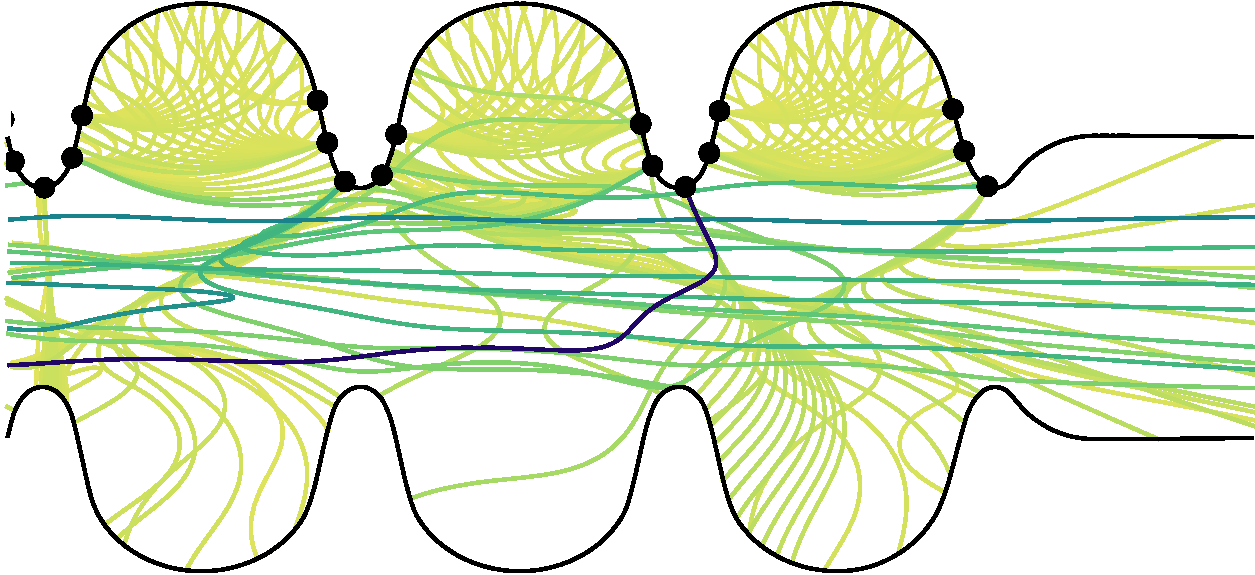
\includegraphics[width=4in]{dark-current.pdf}
  \caption[Dark current tracking.]{
Dark current tracking. Example of where a time based tracker (\vn{time_runge_kutta}) is
useful for simulating particles that can reverse their longitudinal velocity. Here the
tracks drawn are from a simulation of ``dark current'' electrons generated at the
walls of an RF cavity due to the large electromagnetic fields.
}
  \label{f:dark.current}
\end{figure}

\begin{description}

\index{boris!tracking_method}
\item[\vn{Boris}]
Second order Boris Integration\cite{b:boris}. Like \vn{Runge_Kutta},
\vn{Boris} does tracking by integrating the equation of
motion. \vn{Boris} handles both electric and magnetic fields and does
not assume that the particle is ultra--relativistic. \vn{Boris} preserves
conserved quantities more accurately than \vn{Runge_Kutta}.

\index{bmad_standard!tracking_method}
\item[\vn{Bmad_Standard}]
Uses formulas for tracking. The formulas generally use the paraxial
approximation.  The emphasis here is on speed.

\index{custom!tracking_method}
\item[\vn{Custom}]
This method will call a routine \vn{track1_custom} which must be
supplied by the programmer implementing the custom tracking. The
default \vn{track1_custom} supplied with the \bmad release will print
an error message and stop the program if it is called which probably
indicates a program linking problem. See \vn{s:custom.ele} for more details.

\index{linear!tracking_method}
\item[\vn{Linear}]
Linear just uses the 0th order vector with the 1st order 6x6 transfer matrix for an element. Very
simple. Depending upon how the transfer matrix was generated this may or may not be
symplectic. Note: a \vn{linear} tracking method may not be used with \vn{mat6_calc_method} set to
\vn{tracking} since this would give a circular dependency.

\index{MAD!tracking_method}
\item[\vn{MAD}]
This uses the MAD 2nd order transfer map. This method is not able to
handle element misalignments or kicks, and becomes inaccurate as the
particle energy deviates from the reference energy. MAD tracking is
generally only used for testing purposes. Note: Thanks to CERN and
Frank Schmidt for permission to use the MAD tracking code within
\bmad.

\index{runge_kutta!tracking_method}
\item[\vn{runge_kutta}]
This uses a 4\Th order Runge Kutta integration algorithm with adaptive
step size control.  This is essentially the \vn{ODEINT} subroutine
from Numerical Recipes\cite{b:nr}. This may be slow but it should be
accurate. This method is non-symplectic. \vn{Warning:} When using
\vn{custom} fields, if the fields do not obey Maxwell's equation,
there is the possibility of the \vn{runge_kutta} tracking halting mid
way through an element. See section~\sref{s:integ} for more details.

\index{symp_lie_Bmad!tracking_method}
\item[\vn{Symp_Lie_Bmad}]
Symplectic tracking using a Hamiltonian with Lie operation techniques.
This is similar to \vn{Symp_Lie_PTC} (see below) except this uses a
\bmad routine. By bypassing some of the generality inherent in PTC
(\sref{s:ptc.intro}), \vn{Symp_Lie_Bmad} achieves about a factor of 10
improvement in speed over \vn{Symp_Lie_PTC}.

\index{symp_lie_ptc!tracking_method}
\item[\vn{Symp_Lie_PTC}]
Symplectic tracking using a Hamiltonian with Lie operator techniques.
This uses \'Etienne Forest's PTC (\sref{s:ptc.intro}) software for the
calculation. This method is symplectic but can be slow. Exceptions: The tracking is
not symplectic when tracking through and element with an associated electric field
and when tracking through a \vn{taylor} element. 

\index{symp_map!tracking_method}
\item[\vn{Symp_Map}]
This uses a partially inverted, implicit Taylor map. The calculation
uses \'Etienne Forest's PTC software (\sref{s:ptc.intro}).  Since the
map is implicit, a Newton search method must be used. This will slow
things down from the Taylor method but this is guaranteed
symplectic. Note: Due to memory limitations in PTC, the number of
elements using symp_map is limited to be of order 50.

\index{taylor!tracking_method}
\item[\vn{Taylor}]
This uses a Taylor map generated from the PTC (\sref{s:ptc.intro})
package. Generating the map may take time but once you have it it
should be very fast. One possible problem with using a Taylor map is
that you have to worry about the accuracy if you do tracking at points
that are far from the expansion point about which the map was
made. This method is non-symplectic away from the expansion
point. Whether the Taylor map is generated taking into account the
offset an element has is governed by the \vn{taylor_map_includes_offsets}
attribute (\sref{s:mapoff}).  

The order of a Taylor map is set by the \vn{parameter[taylor_order]}
parameter (\sref{s:param}).

Note: Taylor maps for \vn{match} elements are limited to first order.

\index{time_runge_kutta!tracking_method}
\item[\vn{Time_Runge_Kutta}]
This method uses time as the independent variable instead of the longitudinal $z$
position. The advantage of this method is that it can handle particles which reverse
direction longitudinally.  One use for this method is ``dark current'' tracking where, as
illustrated in \fig{f:dark.current}, low energy particles generated at the vacuum chamber
walls can be found traveling in all directions. Notice that \vn{time_runge_kutta} is
different from using \vn{absolute time tracking} as explained in \sref{s:rf.time}.

\end{description}

%----------------------------------------------------------------------------

\index{ab_multipole}\index{beambeam}\index{bend_sol_quad}\index{custom}
\index{drift}\index{ecollimator}\index{elseparator}\index{hkicker}
\index{instrument}\index{kicker}\index{lcavity}\index{marker}
\index{match}\index{monitor}\index{multipole}\index{octupole}
\index{patch}\index{quadrupole}\index{rbend}\index{rcollimator}
\index{rfcavity}\index{sbend}\index{sextupole}\index{solenoid}
\index{sol_quad}\index{taylor}\index{vkicker}\index{wiggler}\index{capillary}
\index{element!table of class types}
\begin{table}[pht]
\centering {
\begin{tabular}{lcccccccccccc} \toprule
\rule{0pt}{80pt} 
{\em Element Class} &
\begin{sideways}\vn{Bmad_Standard}\end{sideways} &
\begin{sideways}\vn{Boris}\end{sideways} &
\begin{sideways}\vn{Custom}\end{sideways} &
\begin{sideways}\vn{Linear}\end{sideways} &
\begin{sideways}\vn{MAD}\end{sideways} &
\begin{sideways}\vn{Runge_Kutta}\end{sideways} &
\begin{sideways}\vn{Symp_Lie_Bmad}\end{sideways} &
\begin{sideways}\vn{Symp_Lie_PTC}\end{sideways} &
\begin{sideways}\vn{Symp_Map}\end{sideways} &
\begin{sideways}\vn{Taylor}\end{sideways} &
\begin{sideways}\vn{Time_Runge_Kutta}\end{sideways} &
\\ \midrule
%                               BS   B   C   L   M   RK    SLB   SLP   SM     T   TRK
  \vn{ab_multipole}            & D &   & X & X &   &     &     &  X  &  X  &  X  &    \\  
  \vn{ac_kicker}               & D & X & X & X &   &  X  &     &     &     &     & X  \\  
  \vn{beambeam}                & D &   & X & X &   &     &     &     &     &     &    \\  
  \vn{bend_sol_quad}           &   &   & X &   &   &     &  D  &     &     &     &    \\  
  \vn{capillary}               & D &   & X &   &   &     &     &     &     &     &    \\  
  \vn{crystal}                 & D &   & X &   &   &     &     &     &     &     &    \\  
  \vn{custom}                  &   & X & D & X &   &  X  &     &     &     &     & X  \\  
  \vn{drift}                   & D & X & X & X & X &  X  &     &  X  &  X  &  X  & X  \\  
  \vn{e_gun}                   &   &   & X &   &   &     &     &     &     &     & D  \\  
  \vn{ecollimator}             & D & X & X & X &   &  X  &     &  X  &  X  &  X  & X  \\  
  \vn{elseparator}             & D & X & X & X & X &  X  &     &  X  &  X  &  X  & X  \\  
  \vn{em_field}                &   & X & X &   &   &  D  &     &     &     &     & X  \\  
  \vn{floor_shift}             & D &   & X &   &   &     &     &     &     &     &    \\  
  \vn{hkicker}                 & D & X & X & X &   &  X  &     &  X  &  X  &  X  & X  \\  
  \vn{instrument}              & D & X & X & X &   &  X  &     &  X  &  X  &  X  & X  \\  
  \vn{kicker}                  & D & X & X & X &   &  X  &     &  X  &  X  &  X  & X  \\  
  \vn{lcavity}                 & D & X & X & X &   &  X  &     &  X  &  X  &  X  & X  \\  
  \vn{marker}                  & D &   & X & X &   &     &     &  X  &  X  &  X  &    \\  
  \vn{match}                   & D &   & X &   &   &     &     &     &     &  *  &    \\ 
  \vn{monitor}                 & D & X & X & X &   &  X  &     &  X  &  X  &  X  & X  \\  
  \vn{mirror}                  & D &   & X &   &   &     &     &     &     &     &    \\  
  \vn{multipole}               & D &   & X & X &   &     &     &  X  &  X  &  X  &    \\  
  \vn{multilayer}              & D &   & X &   &   &     &     &     &     &     &    \\  
  \vn{octupole}                & D & X & X & X &   &  X  &     &  X  &  X  &  X  & X  \\ 
  \vn{patch}                   & D &   & X &   &   &  X  &     &  X  &     &  X  &    \\ 
  \vn{quadrupole}              & D & X & X & X & X &  X  &  X  &  X  &  X  &  X  & X  \\ 
  \vn{rbend}                   & D &   & X & X & X &     &     &  X  &  X  &  X  &    \\ 
  \vn{rcollimator}             & D & X & X & X &   &  X  &     &  X  &  X  &  X  & X  \\ 
  \vn{rfcavity}                & D & X & X & X & X &  X  &     &  X  &  X  &  X  & X  \\ 
  \vn{sad_mult}                & D &   & X & X &   &     &     &  X  &  X  &  X  &    \\
  \vn{sample}                  & D &   & X &   &   &     &     &     &     &     &    \\
  \vn{sbend}                   & D &   & X & X & X &  X  &     &  X  &  X  &  X  & X  \\ 
  \vn{sextupole}               & D & X & X & X & X &  X  &     &  X  &  X  &  X  & X  \\ 
  \vn{solenoid}                & D & X & X & X & X &  X  &  X  &  X  &  X  &  X  & X  \\ 
  \vn{sol_quad}                & D & X & X & X &   &  X  &  X  &  X  &  X  &  X  & X  \\ 
  \vn{taylor}                  &   &   & X & X &   &     &     &  X  &     &  D  &    \\ 
  \vn{vkicker}                 & D & X & X & X &   &  X  &     &  X  &  X  &  X  & X  \\ 
  \vn{wiggler} (map type)      &   & X & X & X &   &  X  &  X  &  X  &  X  &  X  & X  \\
  \vn{wiggler} (periodic type) & D & X & X & X &   &X$^a$&X$^a$&X$^a$&X$^a$&X$^a$&    \\ \bottomrule
   \multicolumn{12}{l}{$^a$See \sref{s:wiggler.periodic} for more details} \\
\end{tabular}
} 
\caption[Table of available {\bf tracking_method}\ switches for a
given element class.]{Table of available {\bf tracking_method}\
switches for a given element class. ``D'' denotes the default
method. ``X'' denotes an available method. ``*'' denotes that the
Taylor map will only be first order. 
}

\label{t:track.methods}
\end{table}

\vfill \break

%----------------------------------------------------------------------------
\section{Linear Transfer Map Methods}
\label{s:xfer}
\index{mat6_calc_method|hyperbf}

The \vn{mat6_calc_method} attribute sets how the 6x6 Jacobian transfer
matrix for a given element is computed.  Table~\ref{t:mat6.methods}
gives which methods are available for each type of element.

\index{sympliectify}
\index{taylor_map_includes_offsets}
In addition to the \vn{mat6_calc_method} switch, 
two element attributes that can affect the way the transfer matrix is
calculated are \vn{symplectify} and \vn{taylor_map_includes_offsets}. These are
discussed in sections \sref{s:symp} and \sref{s:mapoff} respectively.

For methods that do not necessarily produce a symplectic matrix the
\vn{symplectify} attribute of an element can be set to \vn{True} to
solve the problem. See \sref{s:symp.method}. 

Symplectic integration is like ordinary integration of a function f(x)
but what is integrated here is a Taylor map. Truncating the map to
0\Th order gives the particle trajectory and truncating to 1\St\
order gives the transfer matrix (Jacobian).  The order at which a
Taylor series is truncated at is set by \vn{taylor_order} (see
\sref{s:param}. Like ordinary integration there are various
formulas that one can use to do symplectic integration. In \bmad (or
more precisely in PTC (\sref{s:ptc.intro})) you can use one of 3 methods. This is
set by \vn{integrator_order}.  \vn{integrator_order} = n where $n$ is
allowed by PTC to be 2, 4, or 6. With an integration order of $n$ the
error in an integration step scales as $dz^n$ where $dz$ is step
size. The step size $dz$ is set by the length of the element and the
value of \vn{ds_step}. Remember, as in ordinary integration, higher
integration order does not necessarily imply higher accuracy.

\begin{description}

\index{bmad_standard!mat6_calc_method}
\item[\vn{Bmad_Standard}]
Uses formulas for the calculation. The formulas generally use the
paraxial approximation. The emphasis here is on speed.

\index{custom!mat6_calc_method}
\item[\vn{Custom}]
This method will call a routine \vn{make_mat6_custom} which must be
supplied by the programmer implementing the custom transfer matrix
calculation. The default \vn{make_mat6_custom} supplied with the
\bmad release will print an error message and stop the program if it
is called which probably indicates a program linking problem.
See \vn{s:custom.ele} for more details.

\index{MAD!mat6_calc_method}
\item[\vn{MAD}]
This uses the MAD 2nd transfer map. This method is not able to
handle element misalignments or kicks, and becomes inaccurate as the
particle energy deviates from the reference energy. MAD tracking is
generally only used for testing purposes. Thanks must be given
to CERN and Frank Schmidt for permission to use the MAD tracking code
within \bmad.

\index{static!mat6_calc_method}
\item[\vn{Static}]
This prevents the transfer matrix from being recomputed.
Using \vn{Static} in the input file is generally not a good idea since
it prevents the matrix from being computed in the first place.
Typically \vn{Static} is used internally in a program to prevent recomputation.

\index{symp_lie_bmad!mat6_calc_method}
\item[\vn{Symp_Lie_Bmad}]
A symplectic calculation using a Hamiltonian with Lie operator
techniques.  This is similar to \vn{Symp_Lie_PTC} (see below) except
this uses a \bmad routine. By bypassing some of the generality
inherent in PTC, \vn{Symp_Lie_Bmad} achieves about a factor
of 10 improvement in speed over \vn{Symp_Lie_PTC}. However,
\vn{Symp_Lie_Bmad} cannot generate maps above first order.

\index{symp_lie_ptc!mat6_calc_method}
\item[\vn{Symp_Lie_PTC}]
Symplectic integration using a Hamiltonian and Lie operators.
This uses the PTC (\sref{s:ptc.intro}) software for the calculation.
This method is symplectic but can be slow. Exceptions: The tracking is
not symplectic when tracking through and element with an associated electric field
and when tracking through a \vn{taylor} element.

\index{symp_map!tracking_method}
\item[\vn{Symp_Map}]
This uses a partially inverted, implicit Taylor map. The calculation
uses \'Etienne Forest's PTC software (\sref{s:ptc.intro}).  Since the map is implicit, a Newton
search method must be used. This will slow things down from the Taylor
method but this is guaranteed symplectic. Note: Due to memory limitations
in PTC, the number of elements using symp_map is limited to be of order 50.

\index{taylor!mat6_calc_method}
\item[\vn{Taylor}]
This uses a Taylor map generated from \'Etienne's PTC
package. Generating the map may take time but once you have it it
should be very fast. One possible problem with using a Taylor map is
that you have to worry about the accuracy if you do a calculation at
points that are far from the expansion point about which the map was
made. This method is non-symplectic away from the expansion
point. Whether the Taylor map is generated taking into account the
offset an element has is governed by the \vn{taylor_map_includes_offsets}
attribute (\sref{s:mapoff}). \vn{bmad_standard} and \vn{taylor}
tracking methods are identical. Note: Taylor maps for \vn{match}, and
\vn{patch} elements are limited to first order.

The order of a Taylor map is set by the \vn{parameter[taylor_order]}
parameter (\sref{s:param}).

\index{tracking!mat6_calc_method}
\item[\vn{Tracking}]
This uses the tracking method set by \vn{tracking_method} to track 6 particles around the central
orbit. This method is susceptible to inaccuracies caused by nonlinearities. Furthermore this method
is almost surely slow. While non--symplectic, the advantage of this method is that it is directly
related to any tracking results. Note: a \vn{linear} tracking method may not be used with
\vn{mat6_calc_method} set to \vn{tracking} since this would give a circular dependency.

\end{description}

\index{ab_multipole}\index{beambeam}\index{bend_sol_quad}\index{custom}
\index{drift}\index{ecollimator}\index{elseparator}\index{hkicker}
\index{instrument}\index{kicker}\index{lcavity}\index{marker}
\index{match}\index{monitor}\index{multipole}\index{octupole}
\index{patch}\index{quadrupole}\index{rbend}\index{rcollimator}
\index{rfcavity}\index{sbend}\index{sextupole}\index{solenoid}
\index{sol_quad}\index{taylor}\index{vkicker}\index{wiggler}
\index{crystal}\index{capillary}
\begin{table}[pth]
\centering {
\begin{tabular}{lcccccccc} \toprule
\rule{0pt}{80pt} &
\begin{sideways}\vn{Bmad_Standard}\end{sideways} &
\begin{sideways}\vn{Custom}\end{sideways} &
\begin{sideways}\vn{MAD}\end{sideways} &
\begin{sideways}\vn{Static}\end{sideways} &
\begin{sideways}\vn{Symp_Lie_Bmad}\end{sideways} &
\begin{sideways}\vn{Symp_Lie_PTC}\end{sideways} &
\begin{sideways}\vn{Taylor}\end{sideways} &
\begin{sideways}\vn{Tracking}\end{sideways}
\\ \midrule
%                               BS   C   M  Stat SLB   SLP   Tlr  Trk 
  \vn{ab_multipole}            & D & X &   & X &     &  X  &  X  & X \\  
  \vn{ac_kicker}               &   & X &   & X &     &  X  &  X  & D \\  
  \vn{beambeam}                & D & X &   & X &     &     &     & X \\  
  \vn{bend_sol_quad}           &   & X &   & X &  D  &     &     & X \\  
  \vn{capillary}               & D & X &   & X &     &     &     & X \\  
  \vn{crystal}                 & D & X &   & X &     &     &     & X \\  
  \vn{custom}                  &   & D &   & X &     &     &     & X \\  
  \vn{drift}                   & D & X & X & X &     &  X  &  X  & X \\  
  \vn{e_gun}                   &   & X &   & X &     &     &     & D \\  
  \vn{ecollimator}             & D & X &   & X &     &  X  &  X  & X \\  
  \vn{elseparator}             & D & X & X & X &     &  X  &  X  & X \\  
  \vn{em_field}                &   & X &   & X &     &     &     & D \\  
  \vn{floor_shift}             & D & X &   & X &     &     &     & X \\  
  \vn{hkicker}                 & D & X &   & X &     &  X  &  X  & X \\  
  \vn{instrument}              & D & X &   & X &     &  X  &  X  & X \\  
  \vn{kicker}                  & D & X &   & X &     &  X  &  X  & X \\  
  \vn{lcavity}                 & D & X &   & X &     &  X  &  X  & X \\  
  \vn{marker}                  & D & X &   & X &     &  X  &  X  & X \\  
  \vn{match}                   & D & X &   & X &     &     &     & X \\  
  \vn{mirror}                  & D & X &   & X &     &     &     & X \\  
  \vn{monitor}                 & D & X &   & X &     &  X  &  X  & X \\  
  \vn{multipole}               & D & X &   & X &     &  X  &  X  & X \\  
  \vn{multilayer_mirror}       & D & X &   & X &     &     &     & X \\  
  \vn{octupole}                & D & X &   & X &     &  X  &  X  & X \\ 
  \vn{patch}                   & D & X &   & X &     &  X  &  X  & X \\ 
  \vn{quadrupole}              & D & X & X & X &  X  &  X  &  X  & X \\ 
  \vn{rbend}                   & D & X & X & X &     &  X  &  X  & X \\ 
  \vn{rcollimator}             & D & X &   & X &     &  X  &  X  & X \\ 
  \vn{rfcavity}                & D & X & X & X &     &  X  &  X  & X \\ 
  \vn{sad_mult}                & D & X &   & X &     &  X  &  X  & X \\ 
  \vn{sample}                  & D & X &   & X &     &     &     & X \\ 
  \vn{sbend}                   & D & X & X & X &     &  X  &  X  & X \\ 
  \vn{sextupole}               & D & X & X & X &     &  X  &  X  & X \\ 
  \vn{solenoid}                & D & X & X & X &  X  &  X  &  X  & X \\ 
  \vn{sol_quad}                & D & X & X & X &  X  &  X  &  X  & X \\ 
  \vn{taylor}                  &   & X &   & X &     &  X  &  D  &   \\ 
  \vn{vkicker}                 & D & X &   & X &     &  X  &  X  & X \\ 
  \vn{wiggler}                 & D & X &   & X &X$^a$&X$^a$&X$^a$& X \\ \bottomrule
  \multicolumn{9}{l}{$^a$See \sref{s:wiggler.periodic} for more details} \\
\end{tabular}
}
\caption[Table of available \vn{mat6_calc_method}\ switches for a
given element class.]{Table of available \vn{mat6_calc_method}\
switches for a given element class. ``D'' denotes the default
method. ``X'' denotes an available method.}

\label{t:mat6.methods}
\end{table}

\vfill \break

%----------------------------------------------------------------------------
\section{Spin Tracking Methods}
\label{s:spin.methods}
\index{spin tracking!methods}
\index{spin_tracking_method}

The \vn{spin_tracking_method} attribute of an elements sets the algorithm that is used for
tracking a particle's spin (\sref{s:spin.dyn}) through that element.
Table~\ref{t:spin.methods} gives which methods are available for each type of element.

Possible \vn{spin_tracking_method} settings are:
\begin{description}

\index{custom!spin_tracking_method}
\item[\vn{Custom}] \Newline
This method will call a routine \vn{track1_spin_custom} which must be supplied by the
programmer implementing the custom spin tracking calculation. See \vn{s:custom.ele} for
more details.

\index{tracking!mat6_calc_method}
\item[\vn{Tracking}] \Newline
How spin is tracked here will depend also on the setting of \vn{tracking_method}. If
\vn{tracking_method} is set to \vn{boris}, \vn{runge_kutta}, or \vn{time_runge_kutta} the
spin will be tracked along with the phase space particle coordinates using the local
fields. For \vn{tracking_method} set to \vn{symp_lie_ptc}, the spin tracking will use
\vn{PTC}.  For all other \vn{tracking_method}s, the spin will be tracked using the
``\vn{bmad_standard}'' spin tracking method which involves thick element formulas which generally
will be faster but less accurate than the other methods.

\index{symp_lie_ptc!spin_tracking_method}
\item[\vn{Symp_Lie_PTC}] \Newline
Symplectic integration using a Hamiltonian and Lie operators.  This uses \'Etienne's PTC
software for the calculation.  This method is symplectic but can be slow.

\end{description}

Since speed may be an issue, \bmad has an global parameter called
\vn{spin_tracking_on} which is part of the \vn{bmad_com} instance
(\sref{s:bmad.com}) that determines whether spin is tracked or not.

\index{spin_fringe_on}
The \vn{spin_fringe_on} element attribute (\sref{s:fringe.at}) can be used to toggle
whether the fringe fields of an element affect the spin.

Example:
\begin{example}
  q: quadrupole, spin_tracking_method = symp_lie_ptc
\end{example}


\index{ab_multipole}\index{beambeam}\index{bend_sol_quad}\index{custom}
\index{drift}\index{ecollimator}\index{elseparator}\index{hkicker}
\index{instrument}\index{kicker}\index{lcavity}\index{marker}
\index{match}\index{monitor}\index{multipole}\index{octupole}
\index{patch}\index{quadrupole}\index{rbend}\index{rcollimator}
\index{rfcavity}\index{sbend}\index{sextupole}\index{solenoid}
\index{sol_quad}\index{taylor}\index{vkicker}\index{wiggler}
\index{crystal}\index{capillary}
\begin{table}[pth]
\centering {
\begin{tabular}{lcccc} \toprule
\rule{0pt}{80pt} &
\begin{sideways}\vn{Custom}\end{sideways} &
\begin{sideways}\vn{Symp_Lie_PTC}\end{sideways} &
\begin{sideways}\vn{Tracking}\end{sideways}
\\ \midrule
%                                C  SLP Trk 
  \vn{ab_multipole}            & X &   & D \\  
  \vn{ac_kicker}               & X &   & D \\  
  \vn{beambeam}                & X &   &   \\  
  \vn{bend_sol_quad}           & X & X & D \\  
  \vn{capillary}               &   &   &   \\  
  \vn{crystal}                 &   &   &   \\  
  \vn{custom}                  & D &   & X \\  
  \vn{drift}                   & X & X & D \\  
  \vn{e_gun}                   & X &   & D \\  
  \vn{ecollimator}             & X & X & D \\  
  \vn{elseparator}             & X & X & D \\  
  \vn{em_field}                & X &   & D \\  
  \vn{hkicker}                 & X & X & D \\  
  \vn{instrument}              & X & X & D \\  
  \vn{kicker}                  & X & X & D \\  
  \vn{lcavity}                 & X & X & D \\  
  \vn{marker}                  & X & X & D \\  
  \vn{match}                   & X &   &   \\  
  \vn{mirror}                  &   &   &   \\  
  \vn{monitor}                 & X & X & D \\  
  \vn{multipole}               & X & X & D \\  
  \vn{multilayer}              &   &   &   \\  
  \vn{octupole}                & X & X & D \\ 
  \vn{patch}                   & X & X &   \\ 
  \vn{quadrupole}              & X & X & D \\ 
  \vn{rbend}                   & X & X & D \\ 
  \vn{rcollimator}             & X & X & D \\ 
  \vn{rfcavity}                & X & X & D \\ 
  \vn{sad_mult}                & X &   &   \\  
  \vn{sample}                  &   &   &   \\  
  \vn{sbend}                   & X & X & D \\ 
  \vn{sextupole}               & X & X & D \\ 
  \vn{solenoid}                & X & X & D \\ 
  \vn{sol_quad}                & X & X & D \\ 
  \vn{taylor}                  &   &   &   \\ 
  \vn{vkicker}                 & X & X & D \\ 
  \vn{wiggler}                 & X & X & D \\ \bottomrule
\end{tabular}
}

\caption[Table of available \vn{spin_tracking_method}\ switches for a
given element class.]{Table of available \vn{spin_tracking_method}\
switches for a given element class. ``D'' denotes the default
method. ``X'' denotes an available method.}

\label{t:spin.methods}
\end{table}

\vfill \break

%-----------------------------------------------------------------
\section{Integration Methods}
\label{s:integ}
\index{integration methods}

\index{symp_lie_bmad!and Taylor maps}
\index{symp_lie_ptc!and Taylor maps}
\index{taylor!and Taylor maps}
``Integration methods'' are tracking methods that involve integrating
through an element's magnetic and electric fields.  Integration
methods are split into two classes: Those that can track Taylor maps and
those that simply track a particle's position.  The Taylor map methods
are
\begin{example}
  symp_lie_bmad   ! Only to first order
  symp_lie_ptc    ! Uses PTC
  taylor          ! Uses PTC
\end{example}
See section \sref{s:taylor.phys} for more information on Taylor maps
and symplectic integration. The latter two methods involve using the
PTC library (\sref{s:ptc.intro}).

The methods that do not involve Taylor maps are
\index{boris!and Taylor maps}
\index{runge_kutta!and Taylor maps}
\begin{example}
  boris
  runge_kutta
  time_runge_kutta
\end{example}

\index{ds_step}\index{num_steps}\index{integrator_order}
\index{field_calc}\index{csr_calc_on}
there are a number of element attributes that can affect the
calculation. They are
\begin{example}
  ds_step = <Real>              ! Integration step length
  num_steps = <Integer>         ! Number of integration steps.
  integrator_order = <Integer>  ! Integrator order
  field_calc = <Switch>         ! How the field is calculated
  csr_calc_on = <Logical>       ! Coherent Synchrotron Radiation on/off.
\end{example}

Example:
\begin{example}
  q1: quadrupole, l = 0.6, tracking_method = bmad_standard, &
        mat6_calc_method = symp_lie_ptc, ds_step = 0.2, field_calc = custom
\end{example}

\index{ds_step}\index{num_steps}
\index{taylor}\index{symp_lie_ptc}\index{symp_lie_bmad}
\index{runge_kutta}\index{boris}
One way to create a transfer map through an element is to divide the
element up into slices and then to propagate the transfer map slice by
slice.  There are several ways to do this integration. The \vn{boris}
and \vn{runge_kutta} methods integrate the equations of motion to
give the 0\Th order Taylor map which just represents a particle's
orbit.  Symplectic integration\index{symplectic!integration} using Lie
algebraic techniques, on the other hand, can generate Taylor maps to
any order.  The \vn{ds_step} attribute determines the slice thickness.
Alternatively, \vn{num_steps} attribute can be used in place of
\vn{ds_step} to specify the number of slices.
This is applicable to \vn{Boris}, \vn{symp_lie_bmad}, and
\vn{symp_lie_ptc} integration.

\index{integrator_order}
\index{ds_step}\index{symp_lie_bmad}
\vn{integrator_order} is the order of the integration formula for 
\vn{Symp_Lie_PTC}. Possible values are
\begin{example}
  integrator_order = 2 (default), 4, or 6
\end{example}
Essentially, an integration order of $n$ means that the error in an
integration step scales as $dz^{n+1}$ where $dz$ is the slice
thickness.  For a given number of steps a higher order will give more
accurate results but a higher order integrator will take more time per
step. It turns out that for wigglers, after adjusting \vn{ds_step}
for a given accuracy, the order 2 integrator is the fastest. This is
not surprising given the highly nonlinear nature of a wiggler. Note
that \vn{symp_lie_bmad} always uses an order 2 integrator
independent of the setting of \vn{integrator_order}.

\index{ds_step}
\index{runge_kutta}\index{time_runge_kutta}
\index{rel_tol_adaptive_tracking}\index{abs_tol_adaptive_tracking}
The \vn{runge_kutta} and \vn{time_runge_kutta} tracking uses adaptive step
control independent of \vn{ds_step}. These methods use three \vn{bmad_com} parameters
\sref{s:bmad.com}) namely:
\begin{example}
  bmad_com[rel_tol_adaptive_tracking]
  bmad_com[abs_to_adaptive_tracking]
  bmad_com[max_num_runge_kutta_step]
\end{example}
The estimated error of the integration is then bounded by
\begin{example}
  error < abs_tol + |orbit| * rel_tol
\end{example}
lowering the error bounds makes for greater accuracy (as long as round-off 
doesn't hurt) but for slower tracking. 

\index{field_calc}\index{runge_kutta}\index{boris}
The \vn{boris}, and \vn{runge_kutta} tracking all use
as input the electric and magnetic fields of an element. How the EM fields
are calculated is determined by the \vn{field_calc} attribute for an element.
Possible values for \vn{field_calc} are:
\begin{example}
  bmad_standard     ! This is the default
  custom
  fieldmap
\end{example}
\index{custom}\index{runge_kutta}
\vn{Custom} means that the field calculations are done outside of the \bmad software. A program
doing \vn{custom} field calculations will need the appropriate custom routine
(\sref{s:custom.ele}). Elements that set \vn{field_calc} to \vn{fieldmap} need to have a field map
defined (\sref{s:fieldmap}).

The \vn{csr_calc_on} switch toggles on/off Coherent Synchrotron Radiation effects.  The default is
True. CSR effects are only present if the program that is being run is setup to track bunches of
particles (as opposed to single particle tracking).

\vn{Warning:} When tracking a particle through a custom field using \vn{runge_kutta}, it is
important that the field obey Maxwell's equations. Fields that do not obey Maxwell's Equations may
cause the \vn{runge_kutta} adaptive step size control algorithm to take smaller and smaller steps
until the step size becomes so small the tracking will stop. What happens is that the step size
control algorithm takes a step and then takes two half steps over the same region and from this
estimates the error in the calculation. If the error is larger than the allowed tolerance the
control algorithm shortens the step and tries again. A field that does not obey Maxwell's equations
can fool the control algorithm into thinking that the error is always larger than the allowed
tolerance for any finite step size. A typical situation is where the field has an unphysical step
across some boundary.

\index{boris}
The phase space coordinates used with \vn{boris} tracking are not the
standard \bmad coordinates. Rather what is used is
\begin{example}
    (x, p_x/p_0, y, p_y/p_0, s-ct, dE/(cP_0))
\end{example}
At high energy $s-ct = z$ which is the distance of the particle from
the reference particle and $c \, P_0 = v \, E_0/C = E_0$ so that
$dE/cP_0 = dE/E$ giving the standard \bmad coordinates.

\index{ptc_exact_model}\index{ptc_exact_misalign}
When tracking uses the \vn{PTC} library (\sref{s:ptc.intro}), there are two
global parameters that can be set in the lattice file that affect the
calculation. These are:
\begin{example}
  parameter[ptc_exact_model]        = <Logical>  ! "exact" tracking? Default: False
  parameter[ptc_exact_misalignment] = <Logical>  ! "exactly" misalign elements? 
                                                 !    Default: True
\end{example}
The default for \vn{ptc_exact_model} is \vn{False} and the default for
\vn{ptc_exact_misalignment} is \vn{True}. 

The \vn{ptc_exact_model} parameter sets whether PTC uses an ``exact'' model for
tracking. Essentially this means that the paraxial approximation
(\sref{s:mag.hamiltonian}) is made for \vn{ptc_exact_model} set to \vn{False} and is not
made if set to \vn{True}. This can be important, for example, for bend tracking when the
bend radius is small. 

In PTC, exact modeling can be set on an element-by-element basis. Currently \bmad does
not support specifying element-by-element setting of exact modeling. However, PTC does
not have a non-exact tracking option for elements that have an electric field. In this
case, PTC tracking will always be exact independent of the setting of \vn{ptc_exact_model}.
Additionally, for elements with an electric field, tracking will not be symplectic.

The \vn{ptc_exact_misalignment} parameter determines whether
misalignments are handled exactly or whether approximations are made
that will speed up the calculation.

In addition to the above parameters, how the Hamiltonian is split when
tracking with \vn{PTC} can be set for individual elements using the
\vn{ptc_integration_type} parameter. Possible settings of this
parameter are
\begin{example}
  drift_kick    ! See Eq.~(125) of \cite{b:geo.int}
  matrix_kick   ! See Eq.~(132) of \cite{b:geo.int}. Default
  ripken_kick   ! See Eq.~(130) of \cite{b:geo.int}
\end{example}
Example:
\begin{example}
  q2: quad, l = 0.6, k1 = 0.34, ptc_integration_type = drift_kick
\end{example}
A discussion of the different types of integration schemes is given by
Forest\cite{b:geo.int}. The equation that shows the appropriate splitting of the
Hamiltonian for each integration type is referenced in the above list. The
\vn{ripken_kick} type is for benchmarking with the \vn{SixTrack} program and is not
otherwise generally useful. The difference between \vn{drift_kick} and \vn{matrix_kick} is
that with \vn{drift_kick} the quadrupolar part of the magnetic multipole is is included in
the applied kick between drifts while in the \vn{matrix_kick} method the quadrupolar
component is used for the ``matrix'' tracking between kicks. With the
\vn{matrix_kick} method the tune of a machine tends to be insensitive to how many
integration steps (set by \vn{ds_step} or \vn{n_steps}) are used. 

PTC does not implement \vn{matrix_kick} tracking for elements with an electric field.  In
this case, the setting of \vn{ptc_integration_type} is ignored and tracking will be
\vn{drift_kick}. Thus, if an electric field is introduced into an element, more
integration steps may be required to get the correct tune.


%-----------------------------------------------------------------
\section{Symplectify Attribute}
\label{s:symp}
\index{symplectify|hyperbf}

The \vn{symplectify} attribute
\begin{example}
  symplectify = <Logical>
\end{example}
is used to make the transfer matrix for an element symplectic. The
linear transport matrix may be non--symplectic for a number of
reasons.  For example, the linear matrix that comes from expanding a
Taylor Map around any point that is not the origin of the map is
generally not symplectic. The transfer matrix for an element can be
symplectified by setting the \vn{symplectify} attribute to True. See
section~\sref{s:symp.method} for details on how a matrix is
symplectified. The default value of \vn{symplectify}, if it is not
present, is \vn{False}. If it is present without a value then it
defaults to true. Examples:
\begin{example}
  s1: sextupole, l = 0.34                       ! symplectify = False
  s1: sextupole, symplectify = True, l = 0.34   ! symplectify = True
  s1: sextupole, symplectify, l = 0.34          ! symplectify = True
\end{example}

\label{lcavity} Note that for elements like an \vn{lcavity} where the
reference momentum at the downstream end of the element is different
from the upstream end, the transfer matrix is never symplectic. In
this case, ``symplectification'' involves first transforming the
transfer matrix so that the reference momentum is the same upstream
and downstream, then performing symplectification, and finally back
transforming the reference momentum to their original values.

%-----------------------------------------------------------------
\section{taylor_map_include_offsets Attribute}
\label{s:mapoff}
\index{taylor_map_includes_offsets|hyperbf}

The \vn{taylor_map_includes_offsets} attribute sets whether the Taylor map
generated for an element includes the affect due to the elements
(mis)orientation in space. That is, the affect of any pitches, offsets
or tilt (\sref{s:offset}). The default is \vn{True} which means that
the Taylor map will include such effects. 

How \vn{taylor_map_includes_offsets} is set will not affect the results of
tracking or the Jacobian matrix calculation. What is affected is the
speed of the calculations. With \vn{taylor_map_includes_offsets} set to \vn{True}
the Taylor map will have to be recalculated each time an element is
reoriented in space. On the other hand, with \vn{taylor_map_includes_offsets} set
to \vn{False} each tracking and Jacobian matrix calculation will
include the extra computation involving the effect of the
orientation. Thus if an element's orientation is fixed it is faster to
set \vn{taylor_map_includes_offsets} to \vn{True} and if the orientation is
varying it is faster to set \vn{taylor_map_includes_offsets} to \vn{False}.

If the global parameter \vn{bmad_com%conserve_taylor_maps}
(\sref{s:bmad.com}) is set to True (the default), then, if an
element is offset within a program, and if \vn{taylor_map_include_offsets} is set
to True for that element, \bmad will toggle \vn{taylor_map_include_offsets} to
False to conserve the map.

\chapter{Beam Lines and Replacement Lists}
\label{c:sequence}

\index{branch}
This chapter describes how to define the ordered list of elements that
make up a lattice branch (\sref{s:branch.def}).  In a lattice,
branches may be connected together using \vn{fork} or \vn{photon
fork} elements (\vn{s:fork}), or by using \vn{multipass} (\sref{s:multipass}).

%-----------------------------------------------------------------------------
\section{Branch Construction Overview}
\label{s:branch.construct}

\index{list}
A lattice branch is defined in a lattice file using what are called
\vn{beam lines} (\sref{s:lines.wo.arg}) and \vn{replacement lists}
(\sref{s:replace.list}).  The \vn{beam lines} are divided into two
types - lines with (\sref{s:lines.with.arg}) and lines without
(\sref{s:lines.wo.arg}) \vn{replacement arguments}. This essentially
corresponds to the \mad definition of lines and lists. There can be
multiple \vn{beam lines} and \vn{replacement lists} defined in a
lattice file and lines and lists can be nested inside other lines and
lists.

Since lines can be nexted within other lines, The same element name
may be repeated multiple times in a brach. To distinguish between
mutiple elements of the same name, lines and lists may be \vn{tagged} 
(\sref{s:tag}) to produce unique element names.

There will also be a marker element named \vn{END} automatically
placed at the end of the lattice. This end marker will not be
automatically placed in the lattice if a marker named \vn{end} is
defined in the lattice file at the end of the lattice. Additionally, a
\vn{parameter[no_end_marker]} statement (\sref{s:param}) can be used
to suppress the insertion of the end marker.

%-----------------------------------------------------------------------------
\section{Beam Lines and Lattice Expansion}
\label{s:lines.wo.arg}
\index{line|hyperbf}

A \vn{beam line} without arguments has the format
\begin{example}
  label: line = (member1, member2, ...)
\end{example}
where \vn{member1}, \vn{member2}, etc. are either elements, other \vn{beam
lines} or \vn{replacement lists}, or sublines enclosed in parentheses.
Example:
\begin{example}
  line1: line = (a, b, c)
  line2: line = (d, line1, e)
  use, line2
\end{example}
The \vn{use} statement is explained in Section~\sref{s:use}.
This example shows how a \vn{beam line} member can refer to another
\vn{beam line}. This is helpful if the same sequence of elements
appears repeatedly in the lattice. 

The process of constructing the ordered sequences of elements that
comprise the branches of the lattice is called \vn{lattice
expansion}. In the example above, when \vn{line2} is expanded to form
the lattice (in this case there is only one branch so \vn{lattice} and
\vn{branch} can be considered synonymous), the definition of
\vn{line1} will be inserted in to produce the following lattice:
\begin{example}
  beginning, d, a, b, c, e, end
\end{example}
The \vn{beginning} and \vn{end} marker elements are automatically inserted
at the beginning and end of the lattice. The \vn{beginning} element will
always exist but insertion of the \vn{end} element can be supressed by inserting
into the lattice:
\begin{example}
 parameter[no_end_marker] = T    ! See: \sref{s:param}
\end{example}
Lattice expansion occurs at the end when a lattice file has been
parsed or if an \vn{expand_lattice} statement (\sref{s:expand}) is
present.

Each element is assigned an \vn{element index} number starting from 0
for the \vn{beginning} element, 1 for the next element, etc.

In the expanded lattice, any \vn{null_Ele} type elements
(\sref{s:null.ele}) will be discarded. For example, if element \vn{b}
in the above example is a \vn{null_Ele} then the actual expanded
lattice will be:
\begin{example}
  beginning, d, a, c, e, end
\end{example}

\index{reflection of elements}
A member that is a line or list can be ``reflected''
(elements taken in reverse order) if
a negative sign is put in front of it. For example:
\begin{example}
  line1: line = (a, b, c)
  line2: line = (d, -line1, e)
\end{example}
\vn{line2} when expanded gives
\begin{example}
  d, c, b, a, e
\end{example}
Reflecting a subline will also reflect any sublines of the subline. For
example:
\begin{example}
  line0: line = (y, z)
  line1: line = (line0, b, c)
  line2: line = (d, -line1, e)
\end{example}
\vn{line2} when expanded gives
\begin{example}
  d, c, b, z, y, e
\end{example}
\index{sbend}\index{rbend}

A repetition count, which is an integer followed by an asterisk, 
means that the member is
repeated. For example
\begin{example}
  line1: line = (a, b, c)
  line2: line = (d, 2*line1, e)
\end{example}
\vn{line2} when expanded gives
\begin{example}
  d, a, b, c, a, b, c, e
\end{example}
Repetition count can be combined with reflection. For example
\begin{example}
  line1: line = (a, b, c)
  line2: line = (d, -2*line1, e)
\end{example}
\vn{line2} when expanded gives
\begin{example}
  d, c, b, a, c, b, a, e
\end{example}
Instead of the name of a line, subline members can also be given as an explicit 
list using parentheses. For example, the previous example could be rewritten as
\begin{example}
  line2: line = (d, -2*(a, b, c), e)
\end{example}

Lines can be defined in any order in the lattice file so a subline
does not have to come before a line that references it. Additionally,
element definitions can come before or after any lines that reference
them.

A line can have the \vn{multipass} attribute. This is covered in
\sref{s:multipass}.

%-----------------------------------------------------------------------------
\section{Element Reversal}
\label{s:ele.reverse}
\index{element reversal}

An element is \vn{reversed} if particles traveling through it enter at
the ``exit'' end and leave at the ``entrance'' end. Being able to
reverse elements is useful, for example, in describing the interaction
region of a pair of rings where particles of one ring are going in the
opposite direction relative to the particles in the other ring.

Elment reversal is indicated by using a double negative sign ``--''
prefix. The double negative sign prefix can be applied to individual
elements or to a line. If it is applied to a line, the line is both
reflected (same as if a single negative sign is used) and each element
is reflected. For example:
\begin{example}
  line1: line = (a, b, --c)
  line2: line = (--line1)
  line3: line = (c, --b, --a)
\end{example}
In this example, \vn{line2} and \vn{line3} are identical. Notice that
the reversal of a reversed element makes the element unreversed.

Reversed elements, unlike other elements, have their local $z$-axis pointing in the
opposite direction to the local $s$-axis (\sref{s:ref.construct}). This means that there
must be a \vn{reflection patch} (\sref{s:reflect.patch}) between reversed and unreversed
elements. See \sref{s:ex.patch} for an example. Since this complicates matters, it is
generally only useful to employ element reversal in cases where there are multiple
intersectiong lines with particle beams going in opposite directions through some elements
(for example, colliding beam interaction regions). In this case, element reversal is
typically used with \vn{multipass} (\sref{s:multipass}).

Where reversed elements are not needed, it is simple to define elements that are
effectively reversed. For example:
\begin{example}
  b00: bend, angle = 0.023, e1 = ...
  b00_rev: b00, angle = -b00[angle], e1 = -b00[e2], e2 = -b00[e1]
\end{example}
and \vn{b00_rev} serves as a reversed version of \vn{b00}.

Internally, \bmad associates an \vn{orientation} attribute with each element. This
attribute is set to -1 for reversed elements and 1 for unreversed elements. This
attribute. If a program can print out the attributes for an element, checking the
\vn{orientation} attribute will show if an element is reversed or not.

%-----------------------------------------------------------------------------
\section{Beam Lines with Replaceable Arguments}
\label{s:lines.with.arg}
\index{line!with arguments}

\vn{Beam lines} can have an argument list using the following syntax
\begin{example}
  line_name(dummy_arg1, dummy_arg2, ...): LINE = (member1, member2, ...)
\end{example}
The dummy arguments are replaced by the actual arguments when the line is used
elsewhere. For example:
\begin{example}
  line1(DA1, DA2): line = (a, DA2, b, DA1)
  line2: line = (h, line1(y, z), g)
\end{example}
When \vn{line2} is expanded the actual arguments of \vn{line1}, in this
case \vn(y, z), replaces the dummy arguments \vn{(DA1, DA2)} to give for
\vn{line2}
\begin{example}
  h, a, z, b, y, g
\end{example} 
\index{MAD}
Unlike \mad, \vn{beam line} actual arguments can only be elements or \vn{beam lines}. 
Thus the following is not allowed
\begin{example}
  line2: line = (h, line1(2*y, z), g)   ! NO: 2*y NOT allowed as an argument.
\end{example}

%-----------------------------------------------------------------------------
\section{Replacement Lists}
\label{s:replace.list}
\index{list|hyperbf}

When a lattice is expanded, all the lattice members that correspond to
a name of a \vn{replacement list} are replaced successively, by the
members in the \vn{replacement list}. The general syntax is
\begin{example}
  label: LIST = (member1, member2, ...)
\end{example}
For example:
\begin{example}
  list1: list = (a, b, c)
  line1: line = (z1, list1, z2, list1, z3, list1, z4, list1)
  use, line1
\end{example}
When the lattice is expanded the first instance of \vn{list1} in
\vn{line1} is replaced by \vn{a} (which is the first element of
\vn{list1}), the second instance of \vn{list1} is replaced by \vn{b},
etc. If there are more instances of \vn{list1} in the lattice then
members of \vn{list1}, the replacement starts at the beginning of
\vn{list1} after the last member of \vn{list1} is used. In this case the
lattice would be:
\begin{example}
  z1, a, z2, b, z3, c, z4, a
\end{example}
\index{MAD}
Unlike \mad, members of a \vn{replacement list} can only be simple elements 
without reflection or repetition count and not other lines or lists. 
For example the following is not allowed:
\begin{example}
  list1: list = (2*a, b)  ! NO: No repetition count allowed.
\end{example}

%-----------------------------------------------------------------------------
\section{Use Statement}
\label{s:use}

\index{use statement|hyperbf}
The particular line or lines that defines the root branches
(\sref{s:lattice.def}) to be used in the lattice is selected by the
\vn{use} statement. The general syntax is
\begin{example}
  use, line1, line2 ...
\end{example}
For example, \vn{line1} may correspond to one ring and \vn{line2} may
correspond to the other ring of a dual ring colliding beam machine. In
this case, \vn{multipass} (\sref{s:multipass}) will be needed to
describe the common elements of the two rings. Example
\begin{example}
  use, e_ring, p_ring
\end{example}
would pick the lines \vn{e_ring} and \vn{p_ring} for analysis. 
These will be the \vn{root} branches.

\vn{use} statements can come anywhere in the lattice, even before the
definition of the lines they refer to. Additionally, there can be
multiple \vn{use} statements.  The last \vn{use} statement in the file
defines which \vn{line} to use.

The total number of branches in the lattice is equal to the number of lines that appear on
the \vn{use} statement plus the number of \vn{fork} and \vn{photon_fork} elements that branch
to a new branch.

To set such things as the geometry of a branch, beginning Twiss parameters, etc., see Section
\vn{s:beginning}.

%-----------------------------------------------------------------------------
\section{Line and List Tags}
\index{tags for lines and lists|hyperbf}
\label{s:tag}

When a lattice has repeating lines, it can be desirable to differentiate
between repeated elements. This can be done by tagging lines with a \vn{tag}. 
An example will make this clear:
\begin{example}
  line1: line = (a, b)
  line2: line = (line1, line1)
  use, line2
\end{example}
When expanded the lattice would be:
\begin{example}
  a, b, a, b
\end{example}
The first and third elements have the same name ``a'' and the second and fourth
elements have the same name ``b''. Using tags the lattice elements can be given
unique names. lines or lists are tagged  
using brackets \vn{[...]}. The general syntax is:
\begin{example}
  line_name[tag_name]                           ! Syntax for lines
  list_name[tag_name]                           ! Syntax for lists
  replacement_line[tag_name](arg1, arg2, ...)   ! Syntax for replacement lines.
\end{example}
Thus to differentiate the lattice elements in the above example \vn{line2} needs to
be modified using tags:
\begin{example}
  line1: line = (a, b)
  line2: line = (line1[t1], line1[t2])
  use, line2
\end{example}
In this case the lattice elements will have names of the form:
\begin{example}
  tag_name.element_name
\end{example}
In this particular example, the lattice with tagging will be:
\begin{example}
  t1.a, t1.b, t2.a, t2.b
\end{example}
Of course with this simple example one could have just as easily not used tags:
\begin{example}
  t1.a: a;   t2.a: a
  t1.b: b;   t2.b: b
  line1: line = (t1.a, t1.b, t2.a, t2.b)
  use, line2
\end{example}
But in more complicated situations tagging can make for compact lattice files.

When lines are nested, the name of an element is formed by concatenating the tags
together with dots in between in the form:
\begin{example}
  tag_name1.tag_name2. ... tag_name_n.element_name
\end{example}
An example will make this clear:
\begin{example}
  list1 = (g, h)
  line1(y, z) = (a, b)
  line2: line = (line1[t1](a, b))
  line3: line = (line2, list1[hh])
  line4: line = (line3[z1], line3[z2])
  use, line4
\end{example}
The lattice elements in this case are:
\begin{example}
  z1.t1.a, z1.t1.b, z1.hh.g, z2.t1.a, z2.t1.b, z1.hh.h 
\end{example}

\index{expand_lattice}
To modify a particular tagged element the lattice must be expanded
first (\sref{s:expand}). For example:
\begin{example}
  line1: line = (a, b)
  line2: line = (line1[t1], line1[t2])
  use, line2
  expand_lattice
  t1.b[k1] = 1.37
  b[k1] = 0.63       ! This statement does not have any effect
\end{example}
After the lattice has been expanded there is no connection between 
the original \vn{a} and \vn{b} elements and the elements in the lattice like
\vn{t1.b}. Thus the last line in the example where the \vn{k1} attribute of\vn{b} 
is modified do not have any effect on the lattice elements. 

\chapter{Superposition, and Multipass}
\label{c:super.multi}

\index{superposition}\index{multipass}
This chapter covers two concepts: \vn{superposition} (\sref{s:super})
and \vn{multipass} (\sref{s:multipass}) \vn{Superposition} is used
when elements overlap spatially.  \vn{Multipass} is used when an
element is ``shared'' between branches such as the interaction region
shared by two storage rings, or when a beam goes through the same
physical element in a branch multiple times as in an energy recovery
linac.

In both cases, \vn{lord} and \vn{slave} elements (\sref{s:lord.slave})
are constructed by \bmad to hold the necessary information. In both
cases, the \vn{lord} elements will represent the ``physical'' element
while the \vn{slave} elements will embody the ``beam path''.

%-----------------------------------------------------------------------------
\section{Superposition}
\label{s:super}
\index{superimpose|hyperbf}

  \begin{figure}[tb]
  \centering 
  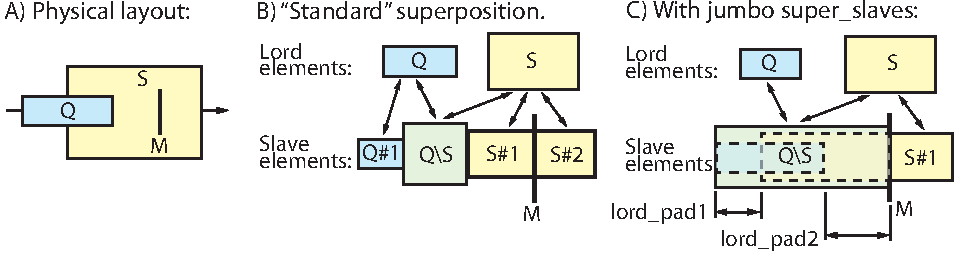
\includegraphics[width=0.95\textwidth]{superimpose-example.pdf} 
  \caption[Superposition example.]
{Superposition example. A) The physical layout involves a quadrupole
partially inside a solenoid. B) The standard superposition procedure
involves creating \vn{super_slave} elements whose edges are at the
boundaries where the physical elements overlap. C) When jumbo
\vn{super_slaves} are created, the \vn{super_slaves} span the entire
space where elements overlap.}
  \label{f:super.ex}
  \end{figure}

In practice the field at a particular point in the lattice may be due
to more than one physical element. One example of this is a quadrupole
magnet inside a larger solenoid magnet as shown in
\fig{f:super.ex}A. \bmad has a mechanism to handle this using what is
called ``superposition''. A simple example shows how this works (also
see section \sref{s:lord.slave}):
\begin{example}
  Q: quad, l = 4
  D: drift, l = 12
  S: solenoid, l = 8, superimpose, ref = Q, ele_origin = beginning
  M: marker, superimpose, ref = S, offset = 1
  lat: line = (Q, D)
  use, lat
\end{example}
The \vn{superimpose} attribute of element \vn{S} superimposes \vn{S}
over the lattice \vn{(Q, D)}. The placement of \vn{S} is such that the
beginning of \vn{S} is coincident with the center of \vn{Q} (this is
is explained in more detail below). Additionally, a marker \vn{M} is
superimposed at a distance of +1~meter from the center of \vn{S}. The
tracking part of the lattice (\sref{s:lord.slave}) looks like:
\begin{example}
        Element   Key         Length  Total     
  1)    Q{\#}1       Quadrupole   2        2
  2)    Q{\B}S       Sol_quad     2        4
  3)    S{\#}1       Solenoid     3        7
  4)    M         Marker       0      
  4)    S{\#}2       Solenoid     3       10
  5)    D{\#}2       Drift        4       14
\end{example}
What \bmad has done is to split the original elements \vn{(Q, D)} at
the edges of \vn{S} and then \vn{S} was split where \vn{M} is
inserted. The first element in the lattice, \vn{Q\#1}, is the part of
\vn{Q} that is outside of \vn{S}. Since this is only part of \vn{Q},
\bmad has put a \vn{\#1} in the name so that there will be no
confusion. (\vn{\#} has no special meaning other than the fact that
\bmad uses it for mangling names). The next element, \vn{Q{\B}S}, is
the part of \vn{Q} that is inside \vn{S}. \vn{Q{\B}S} is a combination
solenoid/quadrupole element as one would expect. \vn{S{\#}1} is the
part of \vn{S} that is outside \vn{Q} but before \vn{M}. This element
is just a solenoid. Next comes \vn{M}, \vn{S{\#}1}, and finally
\vn{D\#2} is the rest of the drift outside \vn{S}.

In the above example, \vn{Q} and \vn{S} will be \vn{super_lord}
elements (\vn{s:lord.slave}) and four elements in the tracking
part of the lattice will be \vn{super_slave} elements. This is
illustrated in \fig{f:super.ex}B.

Notice that the name chosen for the \vn{sol_quad} element \vn{Q{\B}S}
is dependent upon what is being superimposed upon what. If \vn{Q} had
been superimposed upon \vn{S} then the name would have been \vn{S{\B}Q}.

When \bmad sets the element class for elements created from
superpositions, \bmad will set the class of the element to something
other than an \vn{em_field} element (\sref{s:em.field}) if
possible. If no other possibilities exist, \bmad will use
\vn{em_field}. For example, a \vn{quadrupole} superimposed with a
\vn{solenoid} will produce a \vn{sol_quad} element but a \vn{solenoid}
superimposed with a \vn{rfcavity} element will produce an
\vn{em_field} element since there is no other class of element that
can simultaneously handle solenoid and RF fields.

  \begin{figure}[tb]
  \centering 
  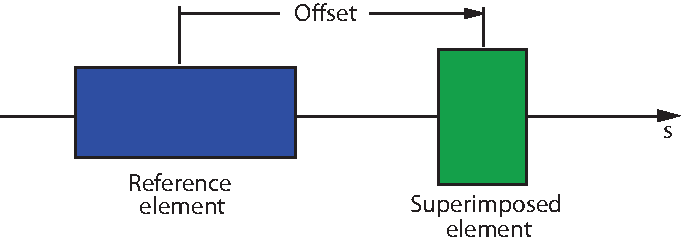
\includegraphics[width=0.8\textwidth]{superimpose.pdf} 
  \caption[Superposition Offset.]{
The superposition offset is the distance from the origin point of the
reference element to the origin point of the element being
superimposed.
  }
  \label{f:superimpose}
  \end{figure}

With the lattice broken up like this \bmad has constructed something
that can be easily analyzed. However, the original elements \vn{Q} and
\vn{S} still exist within the lord section of the lattice. \bmad has
bookkeeping routines so that if a change is made to the \vn{Q} or
\vn{S} elements then these changes can get propagated to the
corresponding slaves. It does not matter which element is
superimposed. Thus, in the above example, \vn{S} could have been put
in the Beam Line (with a drift before it) and \vn{Q} could then have
been superimposed on top and the result would have been the same
(except that the split elements could have different names).

If an element has zero length (for example, a
\vn{marker} element), is superimposed, or is superimposed upon, then the
element will remain in the tracking part of the lattice and there will be
no corresponding lord element. See \fig{f:super.ex}.
 
Superimpose syntax:
\begin{example}
  Q: quad, superimpose, ...       ! Superimpose element Q/
  Q: quad, superimpose = T, ...   ! Same as above.
  Q: quad, ...                    ! First define element Q ...
  Q[superimpose] = T              !   ... and then superimpose.
  Q[superimpose] = F              ! Turn off superposition.
\end{example}

The placement of a superimposed element is illustrated in
\fig{f:superimpose}. The placement of a superimposed element is
determined by three factors: An origin point on the superimposed
element, an origin point on the reference element, and an offset between
the points. The attributes that determine these three quantities are:
\index{ref}\index{offset}
\index{ref_origin}\index{ele_origin}
\begin{example}
  create_jumbo_slave = <Logical>     ! See \sref{s:jumbo.slave}
  ref          = <lattice_element>
  offset       = <length>            ! default = 0
  ele_origin   = <origin_location>   ! Origin pt on element.
  ref_origin   = <origin_location>   ! Origin pt on ref element.
\end{example}
\vn{ref} sets the reference element. If \vn{ref} is not present then
the start of the lattice is used (more precisely, the start of branch
0 (\sref{s:branch.def})). The location of the origin points are
determined by the setting of \vn{ele_origin} and \vn{ref_origin}.  The
possible settings for these parameters are
\begin{example}
  beginning       ! Beginning (upstream) edge of element
  center          ! Center of element. Default.
  end             ! End (downstream) edge of element
\end{example}
\vn{center} is the default setting.
\vn{offset} is the longitudinal offset
between the origin points. The default offset is zero.

Note: There is an old syntax, deprecated but still supported for now,
where the origin points were specified by the appearance of:
\begin{example}
  ele_beginning         ! Old syntax. Do not use.
  ele_center            ! Old syntax. Do not use.
  ele_end               ! Old syntax. Do not use.
  ref_beginning         ! Old syntax. Do not use.
  ref_center            ! Old syntax. Do not use.
  ref_end               ! Old syntax. Do not use.
\end{example}
For example, ``ele_origin = beginning'' in the old syntax would be ``ele_beginning''.

\index{drift}
\index{overlay}\index{group}\index{girder}
The element begin superimposed may be any type of element except
\vn{drift}, \vn{group}, \vn{overlay}, and \vn{girder} control
elements. The reference element used to position a superimposed element
may be a \vn{group} or \vn{overlay} element as long as the \vn{group} or
\vn{overlay} controls the attributes of exactly one element. In this case,
the controlled element is used as the reference element.

\index{geometry}\index{open}
A superimposed element that extends beyond either end of the lattice
will be wrapped around so part of the element will be at the beginning
of the lattice and part of the element will be at the end. For
consistency's sake, this is done even if the \vn{geometry} is set to
\vn{open} (for example, it is sometimes convenient to treat a circular
lattice as linear). Example:
\begin{example}
  d: drift, l = 10
  q: quad, l = 2, superimpose
  machine: line = (d)
  use, machine
\end{example}
The lattice will have three elements in the tracking section:
\begin{example}
        Element   Key           Length
  3)    Q{\#}2       Quadrupole    1
  2)    D{\#}1       Drift         8
  1)    Q{\#}1       Quadrupole    1
\end{example}
The lord section of the lattice will have the element \vn{Q}. 

To superimpose a zero length element ``\vn{S}'' next to a zero length
element ``\vn{Z}'', and to make sure that \vn{S} will be on the
correct side of \vn{Z}, set the \vn{ref_origin} appropriately.
For example:
\begin{example}
  S1: marker, superimpose, ref = Z, ref_origin = beginning
  S2: marker, superimpose, ref = Z, ref_origin = end
  Z: marker
\end{example}
This will place \vn{S1} upstream and \vn{S2} downstream of \vn{Z}.  If
\vn{ref_origin} is not present or set to \vn{center}, the ordering of the
elements will be arbitrary.

\index{drift!superposition}\index{pipe!superposition}
When a superposition is made that overlaps a drift the drift, not
being a "real" element, vanishes. That is, it does not get put in the
lord section of the lattice.  Note that if aperture limits
(\sref{s:limit}) have been assigned to a drift, the aperture limits
can ``disappear'' when the superposition is done. Explicitly, if the
exit end of a drift has been assigned aperture limits, the limits will
disappear if the superimposed element overlays the exit end of the
drift. A similar situation applies to the entrance end of a drift. If
this is not desired, use a \vn{pipe} element instead.

When the attributes of a super_slave are computed from the attributes
of its super_lords, some types of attributes may be ``missing''. For
example, it is, in general, not possible to set appropriate aperture
attributes (\sref{s:limit}) of a super_slave if the lords of the slave
have differing aperture settings. When doing calculations, \bmad will
use the corresponding attributes stored in the lord elements to
correctly calculate things.

%-----------------------------------------------------------------------------
\subsection{Superposition and Sub-Lines}
\label{s:super.sub.line}

Sometimes it is convenient to do simulations with only part of a lattice. The rule for how
superpositions are handled in this case is illustrated in the following example. Consider
a lattice file which defines a \vn{line} called \vn{full} which is defined by two sublines called
\vn{sub1} and \vn{sub2}:
\begin{example}
  sub1: line = {..., ele1, ...}
  sub2: line = {...}
  full: line = {sub1, sub2}
  m1: marker, superimpose, ref = ele1, offset = 3.7
  use, full
\end{example}
Now suppose you want to do a simulation using only the \vn{sub2} line. Rather than edit the
original file, one way to do this would be to create a second file which
overrides the used line:
\begin{example}
  call, file = 'full.bmad'
  use, sub2
\end{example}
where \vn{full.bmad} is the name of the original file. What happens to the superposition
of \vn{m1} in this case? Since \vn{m1} uses a reference element, \vn{ele1}, that is not in
\vn{sub1}, \bmad will ignore the superposition. Even though \bmad will ignore the superposition
of \vn{m1} here, \bmad will check that \vn{ele1} has been defined. If \vn{ele1} has not been
defined, \bmad will assume that there is a typographic error and issue an error message. 

Notice that in this case it is important for the superposition to have an explicit
reference element since without an explicit reference element the superposition is
referenced to the beginning of the lattice. Thus, in the above example, if the
superposition were written like:
\begin{example}
  m1: marker, superimpose, offset = 11.3
\end{example}
then when the \vn{full} line is used, the superposition of \vn{m1} is referenced to the
beginning of \vn{full} (which is the same as the beginning of \vn{sub1}) but when the
\vn{sub2} line is used, the superposition of \vn{m1} is referenced to the beginning
of \vn{sub2} which is not the same as the beginning of \vn{full}.

%-----------------------------------------------------------------------------
\subsection{Jumbo super_slaves}
\label{s:jumbo.slave}

The problem with the way \vn{super_slave} elements are created as
discussed above is that edge effects will not be dealt with properly
when elements with non-zero fields are misaligned. When this is
important, especially at low energy, a possible remedy is to instruct
\bmad to construct ``\vn{jumbo}'' super_slave elements. The general
idea is to create one large \vn{super_slave} for any set of
overlapping elements. Returning to the superposition example at the
start of Section~\sref{s:super}, If the superposition of solenoid \vn{S}
is modified to be
\begin{example}
  S: solenoid, l = 8, superimpose, ref = Q, ele_origin = beginning, 
               create_jumbo_slave = T
\end{example}
The result is shown in \fig{f:super.ex}C. The tracking part of the lattice
will be
\begin{example}
        Element   Key         Length  Total     
  1)    Q{\B}S       Sol_quad     2        4
  2)    M         Marker       0      
  3)    S{\#}2       Solenoid     3       10
  4)    D{\#}2       Drift        4       14
\end{example}
\index{lord_pad1}\index{lord_pad2}
\vn{Q} and part of \vn{S} have been combined into a jumbo
\vn{super_slave} named \vn{Q{\B}S}. Since the \vn{super_lord} elements
of a jumbo \vn{super_slave} may not completely span the slave two
attributes of each lord will be set to show the position of the lord
within the slave. These two attributes are
\begin{example}
  lord_pad1    ! offset at upstream end
  lord_pad2    ! offset at downstream end
\end{example}
\vn{lord_pad1} is the distance between the upstream edge of the jumbo
\vn{super_slave} and a \vn{super_lord}. \vn{lord_pad2} is the distance 
between the downstream edge of a \vn{super_lord} and the downstream edge
of the jumbo \vn{super_slave}. With the present example, the lords have
the following padding:
\begin{example}
          lord_pad1    lord_pad2
  Q            0            3
  S            2            0
\end{example}
The following rule holds for all super lords with and without jumbo slaves:
\begin{example}
  Sum of all slave lengths = lord length + lord_pad1 + lord_pad2
\end{example}

One major drawback of jumbo \vn{super_slave} elements is that the \vn{tracking_method}
(\sref{s:tkm}) will, by necessity, have to be \vn{runge_kutta}, \vn{time_runge_kutta}, or
\vn{boris} and the \vn{mat6_calc_method} (\sref{s:xfer}) will be set to \vn{tracking}.

Notice that the problem with edge effects for non-jumbo
\vn{super_slave} elements only occurs when elements with nonzero
fields are superimposed on top of one another. Thus, for example, one
does not need to use jumbo elements when superimposing a \vn{marker}
element.

\index{field_overlaps}
Another possible way to handle overlapping fields is to use the \vn{field_overlaps}
element attribute as discussed in \sref{s:overlap}.

%-----------------------------------------------------------------------------
\subsection{Changing Element Lengths when there is Superposition}
\label{s:super.length}

When a program is running, if \vn{group} (\sref{s:group}) or
\vn{overlay} (\sref{s:overlay}) elements are used to vary the length
of elements that are involved in superimposition, the results are
different from what would have resulted if instead the lengths of the
elements where changed in the lattice file. There are two reasons for
this. First, once the lattice file has been parsed, lattices can be
``mangled'' by adding or removing elements in a myriad of ways. This
means that it is not possible to devise a general algorithm for
adjusting superimposed element lengths that mirrors what the effect of
changing the lengths in the lattice file.

Second, even if a lattice has not been mangled, an algorithm for
varying lengths that is based on the superimpose information in the
lattice file could lead to unexpected results. To see this consider
the first example in Section~\sref{s:super}. If the length of \vn{S}
is varied in the lattice file, the upstream edge of \vn{S} will remain
fixed at the center of \vn{Q} which means that the length of the
\vn{super_slave} element \vn{Q{\#}1} will be invariant. On the other
hand, if element \vn{S} is defined by 
\begin{example}
  S: solenoid, l = 8, superimpose, offset = 6
\end{example}
This new definition of \vn{S} produces produce exactly the same
lattice as before. However, now varying the length of \vn{S} will
result in the center of \vn{S} remaining fixed and the length of
\vn{Q{\#}1} will not be invariant with changes of the length of
\vn{S}. This variation in behavior could be very confusing since,
while running a program, one could not tell by inspection of the
element positions what should happen if a length were changed.

To avoid confusion, \bmad uses a simple algorithm for varying the
lengths of elements involved in superposition: The rule is that the
length of the most downstream \vn{super_slave} is varied.
With the first example in Section~\sref{s:super}, the \vn{group} \vn{G}
varying the length of \vn{Q} defined by:
\begin{example}
  G: group = \{Q\}, var = \{l\}
\end{example}
would vary the length of \vn{Q{\B}S} which would result in an equal
variation of the length of \vn{S}. To keep the length of \vn{S}
invariant while varying \vn{Q} the individual \vn{super_slave} lengths
can be varied. Example:
\begin{example}
  G2: group = \{Q{\#}1, S{\#}1:-1\}, var = \{l\}
\end{example}
The definition of \vn{G2} must be placed in the lattice file after the
superpositions so that the super slaves referred to by \vn{G2} have
been created. 

In the above example there is another, cleaner, way of achieving
the same result by varying the downstream edge of \vn{Q}:
\begin{example}
  G3: group = \{Q\}, var = \{end_edge\}
\end{example}

%-----------------------------------------------------------------------------
\section{Multipass}
\label{s:multipass}
\index{multipass|hyperbf}

\index{multipass_slave}\index{multipass_lord}
Some lattices have the beam recirculating through the same element
multiple times. For example, an Energy Recovery Linac (ERL) will
circulate the beam back through the LINAC part to retrieve the energy
in the beam. In \bmad, this situation can simulated by designating the LINAC section
as \vn{multipass}. A simple example shows how this
works.
\index{expand_lattice}
\begin{example}
  RF1: lcavity
  linac: line[multipass] = (RF1, ...)
  erl: line = (linac, ..., linac)
  use, erl
  expand_lattice
  RF1\B2[phi0_multipass] = 0.5
\end{example}
The line called \vn{linac} is designated as \vn{multipass}. This
\vn{linac} line appears twice in the line \vn{erl} and \vn{erl} is the
root line for lattice expansion. The lattice constructed from \vn{erl}
will have two \vn{RF1} elements in the tracking part of the lattice:
\begin{example}
  RF1\B1, ..., RF1\B2, ...
\end{example}
Since the two elements are derived from a \vn{multipass} line, they
are given unique names by adding a \vn{{\B}n} suffix. These types of
elements are known as \vn{multipass_slave} elements. In addition, to
the \vn{multipass_slave} elements, there is a \vn{multipass_lord}
element (that doesn't get tracked through) called \vn{RF1} in the lord
part of the lattice (\sref{s:lord.slave}).  Changes to attributes of
the lord \vn{RF1} element will be passed to the slave elements by
\bmad's bookkeeping routines. Assuming that the phase of \vn{RF1\B1}
gives acceleration, to make \vn{RF1\B2} decelerate the
\vn{phi0_multipass} attribute of \vn{RF1\B2} is set to 0.5. This is
the one attribute that \bmad's bookkeeping routines will not touch
when transferring attribute values from \vn{RF1} to its slaves. Notice
that the \vn{phi0_multipass} attribute had to be set after
\vn{expand_lattice} (\sref{s:expand}) is used to expand the lattice
since \bmad does immediate evaluation and \vn{RF1\B2} does not exist
before the lattice is expanded.

Multiple elements of the same name in a multipass line are considered 
physically distinct. Example:
\begin{example}
  m_line: line[multipass] = (A, A, B)
  u_line: line = (m_line, m_line)
  use, u_line
\end{example}
In this example the tracking part of the lattice is
\begin{example}
  A\B1, A\B1, B\B1, A\B2, A\B2, B\B2
\end{example}
In the control section of the lattice there will be two multipass
lords called \vn{A} and one called \vn{B}. [That is, \bmad considers
the lattice to have three physically distinct elements.] The first
\vn{A} lord controls the 1\St and 4\Th elements in the tracking part
of the lattice and the second \vn{A} lord controls the 2\Nd and 5\Th
elements. If \vn{m_line} was {\em not} marked \vn{multipass}, the
tracking part of the lattice would have four \vn{A} and two \vn{B}
elements and there would be no lord elements.

Sublines contained in a multipass line are handled differently
depending upon whether a subline is itself marked \vn{multipass} or
not. When a subline is {\em not} designated \vn{multipass}, the result
is the same as if the elements of the subline where substituted directly
in place of the subline in the containing line. For example:
\begin{example}
  a_line: line = (A)
  m_line: line[multipass] = (a_line, a_line, B)
  u_line: line = (m_line, m_line)
  use, u_line
\end{example}
In this example, \vn{a_line}, which is a subline of the multipass
\vn{m_line}, is {\em not} designated \vn{multipass} and the result
is the same as the previous example where \vn{m_line} was defined
to be \vn{(A, A, B)}. That is, there will be three physical elements
represented by three multipass lords.

When a subline is marked \vn{multipass}, the evaluation of whether the
elements that come from this subline in the expanded lattice are
physical distinct or not is independent of whether the line
containing the subline is marked multipass or not. For example:
\begin{example}
  a_line: line[multipass] = (A)
  m_line: line[multipass] = (a_line, a_line, B)
  u_line: line = (m_line, m_line)
  use, u_line
\end{example}
Here \vn{a_line} is marked as \vn{multipass} so the \vn{A} element
that is contained in it will always represent a single physical 
element. In this case the tracking part of the lattice will be:
\begin{example}
  A\B1, A\B2, B\B1, A\B3, A\B4, B\B2
\end{example}
There will be two lord elements representing the two physically
distinct elements. One multipass lord element will be \vn{A} and this
lord will control the four \vn{A\B n} elements in the tracking part of
the lattice. The \vn{B} lord will control the two \vn{B\B n} elements
in the tracking part of the lattice. Notice that if \vn{m_line} was not
marked as \vn{multipass} in the above example, the four \vn{A\B n} elements
in the tracking part of the lattice would still be considered one physical 
element and would still have a single \vn{A} lord. But in this case,
there would be two \vn{B} elements in the tracking part of the lattice
and no \vn{B} lord.

Multipass lines do not have to be at the same ``level'' in terms of
nesting of lines within lines. Additionally, multipass can be used with line reversal
(\sref{s:ele.reverse}). Example:
\begin{example}
  m_line: line[multipass] = (A, B)
  m2_line: line = (m_line)
  P: patch, ...
  arc: line = (..., P)
  u_line: line = (m_line, arc, --m2_line)
  use, u_line
\end{example}
Here the tracking part of the lattice is
\begin{example}
  A\B1, B\B1, ..., B\B2 (r), A\B2 (r)
\end{example}
The ``(r)'' here just denotes that the element is reversed and is not
part of the name. The lattice will have a multipass lord \vn{A} that
controls the two \vn{A\B n} elements and similarly with \vn{B}. This
lattice represents the case where a particle goes through the m_line
in the ``forward'' direction, gets turned around in the \vn{arc} line,
and then passes back through \vn{m_line} in the reverse direction.
While it is possible to use reflection ``$-$'' (\sref{s:lines.wo.arg})
instead of reversal ``$--$'' (\sref{s:ele.reverse}), reflection here does not make physical
sense.  Needed here is a reversing patch \vn{P} (\sref{s:patch})
between reversed and unreversed elements.

The general rule for deciding how to group multipass elements into slave groups which represent the
same physical element is the following. For any given element in the lattice, this element has some
line it came from. Call this line $L_0$ and denote by $n_0$ the index where the element under
consideration is in $L_0$ line (the first element in $L_0$ has index 1, etc.). The $L_0$ line in
turn came from some other line. Call this line $L_1$ and denote by $n_1$ the position of $L_0$ in
$L_1$. This chain of lines $L_0$, $L_1$, ..., $L_n$ ends at some point and the last (top) line $L_n$
will be one of the root lines listed in the \vn{use} statement (\sref{s:use}). For any given element in the
lattice, starting with $L_0$ and proceeding upwards through the chain, let $L_m$ be the first line
reached that is marked as \vn{multipass}. If no such line exists for a given element then that
element is not part of any multipass grouping and is ignored. All lattice elements that have the
same chain $L_0$, ..., $L_m$ (where $L_m$ is the lowest multipass line) and have the same position
indexes $n_0$, ..., $n_m$ represent the same physical element and are slaved together. For example,
using the example above, the first element of the lattice, \vn{A\B1}, has the chain of lines 
\begin{example}
  \(L_0, n_0\) = m_line, 1
  \(L_1, n_1\) = u_line, 1
\end{example} 
The last element in the lattice, (\vn{A\B2}), has the chain
\begin{example}
  \(L_0, n_0\) = m_line, 1
  \(L_1, n_1\) = m2_line, 1
  \(L_2, n_2\) = u_line, 3
\end{example}
Cutting the chains at the first multipass line, \vn{m_line}, results in identical chains (each with
a single line) so the two elements will be slaved together.

Notice that the global coordinates (\sref{s:global}) of the slaves of
a given multipass lord are not constrained by \bmad to be the same. It
is up to the lattice designer to make sure that the physical positions of
the slaves makes sense (that is, are the same).

%-----------------------------------------------------------------------------
\subsection{The Reference Energy in a Multipass Line}
\label{s:ref.e.multi}

\index{lcavity}
\index{p0c}\index{e_tot}\index{n_ref_pass}
If there are \vn{lcavity} elements in the lattice then the reference energy at a given element may
differ from pass to pass. In this case, the normalized strength (k1, kick, etc.) for magnetic and
electric elements will not be the same from pass to pass. To avoid an ambiguity, all magnetic and
electric elements that are used in a multipass line must have their magnetic or electric field
strength set as the independent attribute (\sref{s:depend}), {\em or} a reference energy
(\sref{s:energy}) must be defined. A reference energy is defined in a multipass element by setting
\vn{e_tot} or \vn{p0c}, or by setting \vn{n_ref_pass} to 1. Exception: For \vn{em_field},
\vn{lcavity}, and \vn{custom} elements where the reference energy may change, \vn{e_tot_start} and
\vn{p0c_start} are used in place of \vn{e_tot} and \vn{p0c}.

Setting \vn{n_ref_pass} to 1 means that the reference energy in the lord element is set using the
reference energy as computed for the first pass slave elements. Previously, \vn{n_ref_pass} could be
set to a number $N$ greater than 1 to indicate that the reference energy would be computed for the
lord using the reference energy of $N$\th pass slaves. However, the bookkeeping proved to be too
complicated so now this is not allowed. Currently, the only permitted values of \vn{n_ref_pass} are
0 and 1 with 0 indicating that the lord reference energy is set directly in the lattice file. Note:
If \vn{e_tot} or \vn{p0c} is set, \vn{n_ref_pass} will default to 0 and it is an error to set it to
1. If neither \vn{e_tot} nor \vn{p0c} is set, \vn{n_ref_pass} will default to 1 and it is an error
to set it to 0.

An example of an ERL lattice with multipass can be found in Section~\sref{s:ex.erl}.

\chapter{Lattice File Global Parameters}

This chapter deals with statements that can be used to set ``global''
parameter values. That is, parameter values that are associated with
the lattice as a whole and not simply associated with a single element.

%-----------------------------------------------------------------------------
\section{Parameter Statements}
\label{s:param}
\index{parameter statement|hyperbf}


\index{lattice}\index{geometry}\index{photon_type}\index{live_branch}
\index{taylor_order}\index{e_tot}
\index{p0c}\index{ran_seed}\index{absolute_time_tracking}
\index{n_part}\index{no_end_marker}
\index{ptc_exact_model}\index{ptc_exact_misalign}
\vn{Parameter} statements are used to set a number of global variables.
If multiple branches are present (\sref{s:branch.def}), these variables pertain
to the \vn{root} branch. The variables that can be set by \vn{parameter} are
\begin{example}
  parameter[absolute_time_tracking]   = <Logical>  ! Absolute time used for RF clock?
  parameter[custom_attributeN]        = <string>   ! Defining custom attributes (\sref{s:cust.att}).
  parameter[default_tracking_species] = <Switch>   ! Default type of tracked particle. 
                                                   !    Default is ref_particle.
  parameter[e_tot]                    = <Real>     ! Reference total Energy. 
                                                   !      Default: 1000 * rest_energy.
  parameter[electric_dipole_moment]   = <Real>     ! Electric dipole moment of tracked particles.
  parameter[live_branch]              = <Logical>  ! Is branch fit for tracking? See below.
  parameter[geometry]                 = <Switch>   ! Open or closed
  parameter[lattice]                  = <String>   ! Lattice name 
  parameter[n_part]                   = <Real>     ! Number of particles in a bunch.
  parameter[no_end_marker]            = <Logical>  ! Default: False.
  parameter[p0c]                      = <Real>     ! Reference momentum.
  parameter[particle]                 = <Switch>   ! Reference species: positron, proton, etc.
  parameter[photon_type]              = <Switch>   ! Incoherent or coherent photons?
  parameter[ptc_exact_model]          = <Logical>  ! PTC to do "exact" tracking?
  parameter[ptc_exact_misalignment]   = <Logical>  ! PTC to "exactly" misalign elements?
  parameter[ptc_max_fringe_order]     = <Integer>  ! Max fringe order. 
                                                   !    Default: 2 => Quadrupole.
  parameter[ran_seed]                 = <Integer>  ! Random number generator init.
  parameter[taylor_order]             = <Integer>  ! Default: 3
  parameter[use_hard_edge_drifts]     = <Logical>
\end{example}

\noindent
Examples
\begin{example}
  parameter[lattice]      = "L9A19C501.FD93S_4S_15KG"
  parameter[geometry]     = closed
  parameter[taylor_order] = 5
  parameter[E_tot]        = 5.6e9    ! eV
\end{example}

  \begin{description}
  \index{absolute_time_tracking}\index{lcavity}\index{rfcavity}
  \item[{parameter[absolute_time_tracking]}] \Newline
The \vn{absolute_time_tracking} switch sets whether the clock for the \vn{lcavity} and
\vn{rfcavity} elements is tied to the reference particle or to uses the absolute time
(\sref{s:rf.time}). A value of \vn{False} (the default) mandates relative time and a value
of \vn{True} mandates absolute time. The exception is that for an \vn{e_gun} element
(\sref{s:e.gun}), absolute time tracking is always used in order to be able to avoid
problems with a zero reference momentum at the beginning of the element.
  \index{custom_attributeN}
  \item[{parameter[custom_attributeN]}] \Newline
For more information on defining custom attributes, see \sref{s:cust.att}.
  \index{live_branch}
  \item[{parameter[live_branch}] \Newline
Setting \vn{live_branch} to \vn{False} (default is \vn{True}) indicates to a program that
no tracking or other analysis of the root branch should be done. This can be useful if the
lattice has multiple branches and analysis of the root branch is not necessary. Other
branches can also be marked as alive/dead using line parameter statements
(\sref{s:beginning}). Note that the \bmad library itself ignores the setting of
\vn{live_branch} and it is up to the program being run to decide if this parameter is
ignored or not. In particular, the \tao program (\sref{s:tao.intro}) {\em will} respect the
setting of \vn{live_branch}.
  \index{default_tracking_species}
  \item[{parameter[default_tracking_species]}] \Newline
The \vn{parameter[default_tracking_species]} switch establishes the
default type of particles to be tracked. Possible setting include
all the settings of \vn{parameter[particle]}. In addition, 
this switch can be set to:
\begin{example}
  ref_particle     ! default
  anti_ref_particle
\end{example}
By default, \vn{default_tracking_species} is set to \vn{ref_particle}
so that the particle being tracked is the same as the reference
particle set by \vn{param[particle]}. In the case, for example,
where there are particles going one way and antiparticles going the another,
\vn{default_tracking_species} can be used to switch between
tracking the particles or antiparticles.
  \index{e_tot}\index{p0c}
  \index{lcavity}\index{patch}
  \item[{parameter[e_tot], parameter[p0c]}] \Newline
The \vn{parameter[e_tot]} and \vn{parameter[p0c]} are the reference
total energy and momentum at the start of the lattice. Each element
in a lattice has an individual reference \vn{e_tot} and \vn{p0c} attributes
which are dependent parameters. The reference energy and momentum will only
change between \vn{LCavity} or \vn{Patch} elements. The starting
reference energy, if not set, will be set to 1000 time the particle
rest energy.  Note: \vn{beginning[e_tot]} and \vn{beginning[p0c]} (\sref{s:beginning}) are
equivalent to \vn{parameter[e_tot]} and \vn{parameter[p0c]}.
  \index{electric_dipole_moment}
  \item[{parameter[electric_dipole_moment]}] \Newline
The \vn{electric_dipole_moment} sets the electric dipole moment value $\eta$ for use
when tracking with spin (\sref{s:spin.dyn}). 
  \index{geometry}\index{closed}\index{open}
  \index{lcavity!and geometry}
  \item[{parameter[geometry]}] \Newline
Valid \vn{geometry} settings are
\begin{example}
  closed  ! Default w/o LCavity element present.
  open    ! Default if LCavity elements present.
\end{example}
A machine with a \vn{closed} geometry is something like a storage ring
where the particle beam recirculates through the machine.  A machine
with an \vn{open} geometry is something like a linac.  In this case,
the initial Twiss parameters need to be specified in the lattice
file. If the \vn{geometry} is not specified, \vn{closed} is the
default. The exception is that if there is an \vn{Lcavity} element
present or the reference particle is a photon, \vn{open} will be the
default.

Notice that by specifying a \vn{closed} geometry it {\em does} not
mean that the downstream end of the last element of the lattice has
the same global coordinates (\sref{s:global}) as the global
coordinates at the beginning. Setting the geometry to \vn{closed}
simply signals to a program to compute closed orbits and periodic
Twiss parameters as opposed to calculating orbits and Twiss parameters
based upon initial orbit and Twiss parameters at the beginning of the
lattice. And indeed, it is sometimes convenient to treat lattices as
closed even though there is no closure in the global coordinate sense.

Note: \vn{geometry} used to be called \vn{lattice_type}, \vn{closed}
used to be called \vn{circular_lattice} and \vn{open} used to be
called \vn{linear_lattice}.
  \index{lattice}
  \item[{parameter[lattice]}] \Newline
Used to set the lattice name. The \vn{lattice} name is stored by \bmad
for use by a program but it does not otherwise effect any \bmad
routines.
  \index{n_part}\index{beambeam}\index{lcavity}
  \item[{parameter[n_part]}] \Newline
The \vn{parameter[n_part]} is the number of particle in a bunch.
it is used with \vn{BeamBeam} elements and is used to calculate the
change in energy through an \vn{Lcavity}. See~\sref{s:lcav} for more
details.
  \index{no_end_marker}\index{end element}
  \item[{parameter[no_end_marker]}] \Newline
The \vn{parameter[no_end_marker]} is use to suppress the automatic inclusion
of a marker named \vn{END} at the end of the lattice (\sref{s:branch.construct}). 
  \item[{parameter[p0c]}] \Newline
See \vn{parameter[e_tot]}.
  \index{particle}
  \index{positron}\index{electron}\index{proton}\index{antiproton}\index{photon}
  \index{muon}\index{antimuon}\index{pion0}\index{pion-}\index{pion+}
  \item[{parameter[particle]}] \Newline
The \vn{parameter[particle]} switch sets the reference species. The possible settings for
this attribute can be divided into four groups. One group are are fundamental
particles. These are:
\begin{example}
  electron,  positron,
  muon,      antimuon,
  proton,    antiproton,
  photon, 
  pion+,      pion0,      pion-
  deuteron
\end{example}
Names for the fundamental particles are {\em not} case sensitive.

Another group are atoms. The general syntax for atoms is:
\begin{example}
  \{\#nnn\}AA\{ccc\}
\end{example}
The curly brackets \{...\} denote optional prefixes and suffixes. \vn{AA} here is the
atomic symbol, \vn{\#nnn} is the number of nucleons, and \vn{ccc} is the charge. Examples:
\begin{example}
  parameter[particle] = \#12C+3       ! Triply charged carbon-12
  parameter[particle] = He--          ! Doubly charged He.
\end{example}
If the number of nucleons is given, the appropriate weight for that isotope is used. If
the number of nucleons is not present, the mass is an average weighted by the isotopic
abundances of the element. The charge may be given by using the appropriate number of plus
(+) or minus (-) signs or by using a plus or minus sign followed by a number. Thus
``\vn{-{-}-}'' is equivalent to ``-3''. Names here are case sensitive. ``@M'' must be used
and not ``@m'' for specifying the mass.

Another group of particles are the ``known'' molecules. The syntax for these are:
\begin{example}
  BBB\{@Mmmmm\}\{ccc\}
\end{example}
\vn{@Mmmmm} is the mass in AMU, \vn{ccc} is the charge, and \vn{BBB} is the molecular
formula. The mass may to specified to hundredths of an AMU. The known molecules are:
\begin{example}
CO       CO2      
D2       D2O      
OH       O2      
H2       H2O      HF
N2       NH2      NH3      
CH2      CH3      CH4      
C2H3     C2H4     C2H5
\end{example}
Like with atoms, if the mass is not specified, the average isotopic mass is used. Examples:
\begin{example}
  C2H3@M28.4+     ! Singly charged C2H3 with mass of 28.4
  CH2             ! Neutral CH2
\end{example}
Like the atomic formulas, molecular formulas are case sensitive.

The last group of particle are particles where only the mass and charge are specified.
The syntax for these are:
\begin{example}
  @Mmmmm\{ccc\}
\end{example}

The setting of the reference particle is
used, for example, to determine the direction of the field in a magnet
and given the normalized field strength (EG: \vn{k1} for a
quadrupole).  Generally, the particles that by default are tracked
through a lattice are the same as the reference particle. This default
behavior can be altered by setting
\vn{parameter[default_tracking_species]}.

  \index{photon_type}
  \item[{parameter[photon_type]}] \Newline
The \vn{photon_type} switch is used to set the type of photons that
are used in tracking. Possible settings are:
\begin{example}
  incoherent    ! Default
  coherent 
\end{example}
The general rule is use incoherent tracking except when there is a
\vn{diffraction_plate} element in the lattice. 

  \index{ptc_exact_model}\index{ptc_exact_misalign}
  \item[{parameter[ptc_exact_model]}] \Newline
The \vn{ptc_exact_model} and \vn{ptc_exact_misalign} switches affect
tracking using the \vn{PTC} library. See \sref{s:integ} for more
details.

  \index{ptc_max_fringe_order}
  \item[{parameter[ptc_max_fringe_order]}] \Newline
When using PTC tracking (\sref{s:ptc.intro}), the
\vn{parameter[ptc_max_fringe_order]} determines the maximum order of
the calculated fringe fields. The default is 2 which means that fringe
fields due to a quadrupolar field. These fields are 3\Rd order in the
transverse coordinates.

  \index{ran_seed}
  \item[{parameter[ran_seed]}] \Newline
For more information on \vn{parameter[ran_seed]} see \sref{s:functions}.

  \index{taylor_order}
  \item[{parameter[taylor_order]}] \Newline
The Taylor order (\sref{s:taylor.phys}) is set by
\vn{parameter[taylor_order]} and is the maximum order for a Taylor map.

  \index{use_hard_edge_drifts}
  \item[{parameter[use_hard_edge_drifts]}] \Newline
The \vn{use_hard_edge_drifts} switch determines if a ``hard edge''
model of certain elements is used. For example, if \vn{runge_kutta}
tracking is used for an \vn{rfcavity} or \vn{lcavity} using a standing
wave model then the cavity length should be a multiple of the RF
wavelength/2. To achieve this, during tracking, the cavity length is
appropriately modified and drifts are inserted at either ends of the
cavity to keep the total length constant. Default is \vn{True}.

  \end{description}

%-----------------------------------------------------------------------------
\section{Beam_Start Statements} 
\label{s:beam.start}
\index{beam_start statement|hyperbf}

\index{e_gun}
\index{x}\index{px}\index{y}\index{py}\index{z}\index{pz}
\index{emittance_a}\index{emittance_b}\index{emittance_z}
\index{field_x}\index{field_y}\index{phase_x}\index{phase_y}
\index{spin_x}\index{spin_y}\index{spin_z}\index{spinor_theta}
\index{spinor_phi}\index{spinor_xi}\index{spinor_polarization}
\vn{Beam_start} statements are used, among other things to set the starting coordinates
for particle tracking. If multiple branches are present (\sref{s:branch.def}), these
variables pertain to the \vn{root} branch.
\begin{example}
  beam_start[x]                   = <Real>   ! Horizontal position.
  beam_start[px]                  = <Real>   ! Horizontal momentum.
  beam_start[y]                   = <Real>   ! Vertical position.
  beam_start[py]                  = <Real>   ! Vertical momentum.
  beam_start[z]                   = <Real>   ! Longitudinal position.
  beam_start[pz]                  = <Real>   ! Momentum deviation. Only for non-photons.
  beam_start[direction]           = +/-1     ! Longitudinal direction of travel.
  beam_start[E_photon]            = <Real>   ! Energy (eV). Only used for photons.
  beam_start[emittance_a]         = <Real>   ! A-mode emittance
  beam_start[emittance_b]         = <Real>   ! B-mode emittance
  beam_start[emittance_z]         = <Real>   ! Z-mode emittance
  beam_start[sig_z]               = <Real>   ! Beam sigma in z-direction
  beam_start[sig_e]               = <Real>   ! Sigma_E/E relative beam energy sigma.
  beam_start[field_x]             = <Real>   ! Photon beam field along x-axis
  beam_start[field_y]             = <Real>   ! Photon beam field along y-axis
  beam_start[phase_x]             = <Real>   ! Photon beam phase along x-axis
  beam_start[phase_y]             = <Real>   ! Photon beam phase along y-axis
  beam_start[t]                   = <Real>   ! Absolute time
  beam_start[spin_x]              = <Real>   ! Spin polarization x-coordinate
  beam_start[spin_y]              = <Real>   ! Spin polarization y-coordinate
  beam_start[spin_z]              = <Real>   ! Spin polarization z-coordinate
  beam_start[spinor_polarization] = <Real>   ! Spin polarization
  beam_start[spinor_theta]        = <Real>   ! Spin angle
  beam_start[spinor_phi]          = <Real>   ! Spin angle
  beam_start[spinor_xi]           = <Real>   ! Spin angle
\end{example}
Normally the absolute time, set by \vn{beam_start[t]}, is a dependent
parameter set by solving \Eq{zbctt} for $t$. The exception is when the
initial velocity is zero. (This can happen if there is an \vn{e_gun}
(\sref{s:e.gun}) element in the lattice). In this case, $z$ must be
zero and $t$ is an independent parameter that can be set.

The longitudinal direction of travel is set by \vn{beam_start[direction]}.  This can be set
to +1 (travel in the +s direction) or -1 for the reverse.  +1 is the default. Generally
\vn{beam_start[direction]} should not be set to -1 since most programs will not be
constructed to handle this situation. To track a particle in the reverse direction see
\sref{s:reverse}. 

For particles with spin, the spin can be specified in one of two ways:
One way is to specify the $(x, y, z)$ spin components using
\vn{spin_x}, \vn{spin_y}, and \vn{spin_z}. The second way is by
specifying the polar angles and magnitude with \vn{spinor_theta},
\vn{spinor_phi}, \vn{spinor_xi}, and \vn{spinor_polarization}. The
relationship between the two spin representations is given by
\Eq{pp1p2}. To prevent ambiguity, only one representation can can be
used in lattice. The default is
\begin{example}
  spinor_polarization = 1
  spinor_theta        = 0
  spinor_phi          = 0
  spinor_xi           = 0

  spin_x              = 0
  spin_y              = 0
  spin_z              = 1
\end{example}

For photons, \vn{px}, \vn{py}, and \vn{pz} are the normalized velocity components
(Cf.~\Eq{xbybzb}). For photons \vn{pz} is a dependent parameter which will be set
so that \Eq{bbb1} is obeyed.


Example
\begin{example}
  beam_start[y] = 2 * beam_start[x]
\end{example}

%-----------------------------------------------------------------------------
\section{Beam Statement}
\index{beam statement|hyperbf}

\index{energy}
\index{particle}
\index{n_part}
\index{MAD!beam statement}
The \vn{beam} statement is provided for compatibility with \mad. The syntax is
\begin{example}
  beam, energy = GeV, pc = GeV, particle = <Switch>, n_part = <Real>
\end{example}
For example
\index{MAD}
\begin{example}
  beam, energy = 5.6  ! Note: GeV to be compatible with \mad
  beam, particle = electron, n_part = 1.6e10
\end{example}
Setting the reference energy using the \vn{energy} attribute is the
same as using \vn{parameter[e_tot]}. Similarly, setting \vn{pc} is
equivalent to setting \vn{parameter[p0c]}. Valid \vn{particle} switches
are the same as \vn{parameter[particle]}.

%--------------------------------------------------------------------------
\section{Beginning and Line Parameter Statements}
\label{s:beginning}
\index{beginning statement|hyperbf}

\index{beta_a}\index{alpha_a}
\index{phi_a}\index{eta_x}
\index{etap_x}\index{beta_b}
\index{alpha_b}\index{phi_b}
\index{eta_y}\index{etap_y}
\index{cmat_ij}\index{e_tot}
\index{p0c}\index{ref_time}
For non--circular lattices, the \vn{beginning} statement can be used to
set the Twiss parameters and beam energy at the beginning of the first lattice branch.
\begin{example}
  beginning[alpha_a]  = <Real>  ! "a" mode alpha
  beginning[alpha_b]  = <Real>  ! "b" mode alpha
  beginning[beta_a]   = <Real>  ! "a" mode beta
  beginning[beta_b]   = <Real>  ! "b" mode beta
  beginning[cmat_ij]  = <Real>  ! C coupling matrix. i, j = \{``1'', or ``2''\} 
  beginning[e_tot]    = <Real>  ! Reference total energy in eV.
  beginning[eta_x]    = <Real>  ! x-axis dispersion
  beginning[eta_y]    = <Real>  ! y-axis dispersion
  beginning[etap_x]   = <Real>  ! x-axis dispersion derivative.
  beginning[etap_y]   = <Real>  ! y-axis dispersion derivative.
  beginning[p0c]      = <Real>  ! Reference momentum in eV.
  beginning[phi_a]    = <Real>  ! "a" mode phase.
  beginning[phi_b]    = <Real>  ! "b" mode phase.
  beginning[ref_time] = <Real>  ! Starting reference time.
  beginning[s]        = <Real>  ! Longitudinal starting position.
\end{example}
\index{e_tot}
The \vn{gamma_a}, \vn{gamma_b}, and \vn{gamma_c} (the coupling gamma
factor) will be kept consistent with the values set. If not set the
default values are all zero.  \vn{beginning[e_tot]} and
\vn{parameter[e_tot]} are equivalent and one or the other may be
set but not both. Similarly, \vn{beginning[p0c]} and
\vn{parameter[p0c]} are equivalent.

\index{x_position}\index{y_position}\index{z_position}
\index{theta_position}\index{phi_position}\index{psi_position}
For any lattice the \vn{beginning} statement can be used to set the
starting floor position of the first lattice branch
(see~\sref{s:global}). The syntax is
\begin{example}
  beginning[x_position]     = <Real>  ! X position
  beginning[y_position]     = <Real>  ! Y position
  beginning[z_position]     = <Real>  ! Z position
  beginning[theta_position] = <Real>  ! Angle on floor
  beginning[phi_position]   = <Real>  ! Angle of attack
  beginning[psi_position]   = <Real>  ! Roll angle
\end{example}
If the floor position is not specified, the default is to place
beginning element at the origin with all angles set to zero.

\index{root branch}\index{branch}
The \vn{beginning} statement is useful in situations where only parameters for
the first branch need be specified. If this is not the case, the parameters for
any branch can be specified using a statement of the form
\begin{example}
  line_name[parameter] = <Value>
\end{example}
This construct is called a \vn{line parameter} statement
Here \vn{line_name} is the name of a line and \vn{parameter} is the
name of a parameter. The parameters that can be set here are the same
parameters that can be set with the \vn{beginning} statement with the additional
parameters from the \vn{parameter} statement:
\index{geometry}\index{particle}\index{default_tracking_species}
\begin{example}
  default_tracking_species
  geometry
  live_branch
  particle
\end{example}
Example:
\begin{example}
  x_ray_fork: fork, to_line = x_ray
  x_ray = (...)
  x_ray[E_tot] = 100
\end{example}

Rules:
  \begin{enumerate}
  \item
The floor position of a line can only be set if the line is used for a 
\vn{root} \vn{branch}. 
  \item
Line parameters statements must come after the associated line. This
rule is similar to the rule that element attribute redefinitions must
come after the definition of the element.
 \end{enumerate}

\chapter{Parameter Structures}
\label{c:param.structs}

A ``structure'' is a collection of parameters.  \bmad has various
structures which can be used for various tasks. For example, the
\vn{beam_init_struct} structure (\sref{s:beam.init}) is used to set
parameters used to initialize particle beams.

A given program may give the user access to some of these structures
so, in order to allow intelligent parameter setting, this chapter
gives an in-depth description of the most common ones.

Each structure has a \vn{``structure name''} (also called a \vn{``type
name''}) which identifies the list of parameters (also called
``components'') in the structure. Associated with a structure there
will be an \vn{``instance''} of this structure and this instance will
have an \vn{``instance name''} which is what the user uses to set
parameters. It is possible to have multiple instances of a
structure. For example, in the situation where a program is simulating
multiple particle beams, there could be multiple \vn{beam_init_struct}
(\sref{s:beam.init}) instances with one for each beam.

\bmad defines uses some structures to hold global parameters. That is,
parameters that shared by all code. Each of these structures has
a single associated instance. These are:
\begin{center}
  \begin{tabular}{ll} \toprule
  Structure           & Instance    \\
  \midrule
  bmad_common_stuct   & bmad_com    \\
  csr_parameter_stuct & csr_param   \\
  \bottomrule
  \end{tabular}
\end{center}
All other structures will have instance names that are program
specific.  That is, see the program documentation for the instance
name(s) used.

To set a particular component of an instance use the syntax
\begin{example}
  instance_name%parameter_name = value
\end{example}
Example:
\begin{example}
  bmad_com%max_aperture_limit = 10
\end{example}
this sets the \vn{max_aperture_limit} parameter of \vn{bmad_com}.

%-----------------------------------------------------------------
\section{Bmad_Common_Struct}
\label{s:bmad.common}
\index{Bmad!general parameters|hyperbf}

The \vn{bmad_common_struct} structure contains a set of global parameters. There is only
one instance (\sref{c:param.structs}) of this structure and this instance has the name
\vn{bmad_com}. The components of this structure along with the default values are:
\index{max_aperture_limit}\index{d_orb(6)}
\index{grad_loss_sr_wake}\index{default_ds_step}
\index{rel_tol_tracking}\index{abs_tol_tracking}
\index{rel_tol_adaptive_tracking}\index{abs_tol_adaptive_tracking}
\index{taylor_order}\index{default_integ_order}
\index{sr_wakes_on}\index{lr_wakes_on}
\index{mat6_track_symmetric}\index{auto_bookkeeper}
\index{space_charge_on}\index{coherent_synch_rad_on}
\index{spin_tracking_on}\index{radiation_damping_on}
\index{radiation_fluctuations_on}\index{be_thread_safe}
\index{absolute_time_tracking_default}
\index{bmad_common_struct|hyperbf}
\begin{example}
  type bmad_common_struct
    real(rp) max_aperture_limit = 1e3          ! Max Aperture.
    real(rp) d_orb(6)           = 1e-5         ! for the make_mat6_tracking routine.
    real(rp) default_ds_step    = 0.2          ! Integration step size.  
    real(rp) significant_length = 1e-10        ! meter 
    real(rp) rel_tol_tracking = 1e-8           ! Closed orbit relative tolerance.
    real(rp) abs_tol_tracking = 1e-10          ! Closed orbit absolute tolerance.
    real(rp) rel_tol_adaptive_tracking = 1e-8  ! Runge-Kutta tracking relative tolerance.
    real(rp) abs_tol_adaptive_tracking = 1e-10 ! Runge-Kutta tracking absolute tolerance.
    real(rp) init_ds_adaptive_tracking = 1e-3  ! Initial step size.
    real(rp) min_ds_adaptive_tracking = 0      ! Minimum step size to use.
    real(rp) fatal_ds_adaptive_tracking = 1e-8 ! Threshold for loosing particles.
    real(rp) sad_eps_scale = 5.0d-3            ! Used in sad_mult step length calc.
    real(rp) sad_amp_max = 5.0d-2              ! Used in sad_mult step length calc.
    integer sad_n_div_max = 1000               ! Used in sad_mult step length calc.
    integer taylor_order = 3                   ! 3rd order is default
    integer default_integ_order = 2            ! PTC integration order
    integer ptc_max_fringe_order = 2           ! PTC max fringe order (2 => Quadrupole !).
    integer max_num_runge_kutta_step = 10000   ! Max num RK steps before particle is lost.
    logical use_hard_edge_drifts = T           ! Insert drifts when tracking through cavity?
    logical sr_wakes_on = T                    ! Short range wake fields?
    logical lr_wakes_on = T                    ! Long range wake fields
    logical mat6_track_symmetric = T           ! symmetric offsets
    logical auto_bookkeeper = T                ! Automatic bookkeeping?
    logical space_charge_on = F                ! Space charge switch
    logical coherent_synch_rad_on = F          ! csr 
    logical spin_tracking_on = F               ! spin tracking?
    logical radiation_damping_on = F           ! Damping toggle.
    logical radiation_fluctuations_on = F      ! Fluctuations toggle.
    logical conserve_taylor_maps = T           ! Enable bookkeeper to set
                                               ! ele%taylor_map_includes_offsets = F?
    logical absolute_time_tracking_default = F ! Default for lat%absolute_time_tracking
    logical aperture_limit_on = T              ! Use aperture limits in tracking.
    logical debug = F                          ! Used for code debugging.
  end type
\end{example}

Note: \vn{bmad_com} parameters may always be set in a lattice file as
discussed in Section~\sref{s:bmad.com}. However, thought must be given
to setting \vn{bmad_com} parameters in a lattice file since that will
affect every program that uses the lattice.

Parameter description:
\begin{description}
\index{aperture_limit_on}
\item[\vn{\%abs_tol_adaptive_tracking}] \Newline
Absolute tolerance to use in adaptive tracking. This is used in
\vn{runge-kutta} and \vn{time_runge_kutta} tracking (\sref{s:integ}).

\item[\vn{\%abs_tol_tracking}] \Newline
Absolute tolerance to use in tracking. Specifically, Tolerance to use
when finding the closed orbit.

\item[\vn{\%aperture_limit_on]}] \Newline
Aperture limits may be set for elements in the lattice
(\sref{s:limit}). Setting \vn{aperture_limit_on} to \vn{False} will
disable all set apertures. \vn{True} is the default.

\item[\vn{\%auto_bookkeeper}] \Newline
Toggles automatic or intelligent bookkeeping. See
section~\sref{s:lat.bookkeeping} for more details.

\item[\vn{\%d_orb}] \Newline 
Sets the orbit displacement used in the routine that calculates the
transfer matrix through an element via tracking.  \vn{%d_orb} needs to
be large enough to avoid significant round-off errors but not so large
that nonlinearities will affect the results. Also see
\vn{%mat6_track_symmetric}.

\item[\vn{\%default_ds_step}] \Newline
Step size for tracking code \sref{c:methods} that uses a fixed step
size. For example, \vn{symp_lie_ptc} and \vn{boris} tracking.

\item[\vn{\%default_integ_order}] \Newline
Order of the the integrator used by \'Etienne Forest's PTC code (\sref{s:libs}).

\item[\vn{\%max_aperture_limit}] \Newline 
Sets the maximum amplitude a particle can have
during tracking. If this amplitude is exceeded, the particle is lost
even if there is no element aperture set. Having a maximum aperture
limit helps prevent numerical overflow in the tracking calculations.

\item[\vn{\%max_num_runge_kutta_step}] \Newline 
The maximum number of steps to take through an element with \vn{runge_kutta} or
\vn{time_runge_kutta} tracking. The default value is 10,000. If the number of steps
reaches this value, the particle being tracked is marked as lost and a warning message is
issued. Under ``normal'' circumstances, a particle will take far fewer steps to track
through an element. If a particle is not through an element after 10,000 steps, it
generally indicates that there is a problem with how the field is defined. That is, the
field does not obey Maxwell's Equations. Especially: discontinuities in the field can
cause problems.

\item[\vn{\%rel_tol_adaptive_tracking}] \Newline
Relative tolerance to use in adaptive tracking. This is used in
\vn{runge_kutta} and \vn{time_runge_kutta} tracking (\sref{s:integ}).

\item[\vn{\%init_ds_adaptive_tracking}] \Newline
Initial step to use for adaptive tracking. This is used in
\vn{runge-kutta} and \vn{time_runge_kutta} tracking (\sref{s:integ}).

\item[\vn{\%min_ds_adaptive_tracking}] \Newline
This is used in \vn{runge-kutta} and \vn{time_runge_kutta} tracking
(\sref{s:integ}). Minimum step size to use for adaptive tracking. If
To be useful, \vn{%min_ds_adaptive_tracking} must be set larger than
the value of \vn{%fatal_ds_adaptive_tracking}. In this case,
particles are never lost due to taking too small a step.

\item[\vn{\%fatal_ds_adaptive_tracking}] \Newline
This is used in \vn{runge-kutta} and \vn{time_runge_kutta} tracking
(\sref{s:integ}).  If the step size falls below the value set for
\vn{%fatal_ds_adaptive_tracking}, a particle is considered lost.
This prevents a program from ``hanging'' due to taking a large number
of extremely small steps. The most common cause of small step size is
an ``unphysical'' magnetic or electric field.

\item[\vn{\%rel_tol_tracking}] \Newline
Relative tolerance to use in tracking. Specifically, Tolerance to use
when finding the closed orbit.

\item[\vn{\%default_integ_order}] \Newline
Order of the the integrator used by \'Etienne Forest's PTC code (\sref{s:libs}).
The order of the PTC integrator is like the order of a Newton-Cotes method.
Higher order means the error term involves a higher order derivative of the field.

\item{ptc_max_fringe_order} \Newline
Maximum order for computing fringe field effects in PTC. 

\item[\vn{\%significant_length}] \Newline
Sets the scale to decide if two length values are significantly
different. For example, The superposition code will not create any
super_slave elements that have a length less then this.

\item[\vn{\%sr_wakes_on}] \Newline
Toggle for turning on or off short-range higher order mode wake field effects.

\item[\vn{\%lr_wakes_on}] \Newline
Toggle for turning on or off long-range higher order mode wake field effects.

\item[\vn{\%mat6_track_symmetric}] \Newline
Toggle to turn off whether the transfer matrix from tracking routine
(\Hyperref{r:twiss.from.tracking}{twiss_from_tracking}) tracks 12 particles at both plus and
minus \vn{%d_orb} values or only tracks 7 particles to save time.

\item[\vn{\%space_charge_on}] \Newline
Toggle to turn on or off the high energy space charge effect in particle tracking
(\sref{s:space.charge}). This is not to be confused with the space charge component of
coherent synchrotron radiation (\sref{s:csr}).

\item[\vn{\%coherent_synch_rad_on}] \Newline
Toggle to turn on or off the coherent space charge calculation.

\item[\vn{\%spin_tracking_on}] \Newline
Determines if spin tracking is performed or not.

\item[\vn{\%taylor_order}] \Newline
Cutoff Taylor order of maps produced by \vn{sym_lie_ptc}.

\item[\vn{\%radiation_damping_on}] \Newline
Toggle to turn on or off effects due to radiation damping in particle tracking.

\item[\vn{\%radiation_fluctuations_on}] \Newline
Toggle to turn on or off effects due to radiation fluctuations in particle tracking.

\item[\vn{\%conserve_taylor_maps}] \Newline
Toggle to determine if the Taylor map for an element include any
element ``misalignments''.  See Section~\sref{s:mapoff} for more
details.

\item[\vn{\%absolute_time_tracking_default}] \Newline
Default setting to be applied to a lattice if
\vn{absolute_time_tracking} (\sref{s:param}) is not specified in a
lattice file. Additionally, if an element that is not associated with a lattice
is tracked, \vn{%absolute_time_tracking_default} will be used to
determine whether absolute time tracking is used. 

To change between absolute and relative time tracking
(\sref{s:rf.time}) after lattice file parsing, the
\vn{%absolute_time_tracking} component of a \vn{lat_struct}
(\sref{s:abs.time}) can be appropriately set.

\item[\vn{\%debug}] \Newline
Used for communication between program units for debugging purposes.

\end{description}

%-----------------------------------------------------------------
\section{Bmad_Com}
\label{s:bmad.com}

\index{bmad_com}
The parameters of the \vn{bmad_com} instance of the
\vn{bmad_common_struct} structure (\sref{s:bmad.common}) can be set in
the lattice file using the syntax
\begin{example}
  bmad_com[parm-name] = value
\end{example}
where \vn{parm-name} is the name of a component of
\vn{bmad_common_struct}. For example:
\begin{example}
  bmad_com[rel_tol_tracking] = 1e-7
\end{example}

Be aware that setting a \vn{bmad_com} parameter value in a lattice
file will affect all computations of a program even if the program
reads in additional lattice files. That is, setting of \vn{bmad_com}
components is ``sticky'' and persists even when other lattice files
are read in. There are two exceptions: A program is always free to
override settings of \vn{bmad_com} parameters. Additionally, a second
lattice file can also override the setting made in a prior lattice
file.
%-----------------------------------------------------------------
\section{Beam_Init_Struct}
\label{s:beam.init}
\index{beam initialization parameters|hyperbf}

\index{beam_init_struct|hyperbf}
Beams of particles are used for simulating inter-bunch intra-bunch
effects. The \vn{beam_init_struct} structure holds parameters which
are used to initialize a beam. The The parameters of this structure
are:
\begin{example}
  type beam_init_struct
    character distribution_type(3)         ! "ELLIPSE", "KV", "GRID", "" (default).
    type (ellipse_beam_init_struct) ellipse(3) ! For ellipse beam distribution
    type (kv_beam_init_struct) KV              ! For KV beam distribution
    type (grid_beam_init_struct) grid(3)       ! For grid beam distribution
    !!! The following are for Random distributions
    character random_engine          ! "pseudo" (default) or "quasi". 
    character random_gauss_converter ! "exact" (default) or "quick". 
    real random_sigma_cutoff = -1    ! -1 => no cutoff used.
    real center_jitter(6) = 0.0      ! Bunch center rms jitter
    real emit_jitter(2)   = 0.0      ! %RMS a and b mode bunch emittance jitter
    real sig_z_jitter     = 0.0      ! bunch length RMS jitter 
    real sig_e_jitter     = 0.0      ! energy spread RMS jitter 
    integer n_particle = 0               ! Number of simulated particles per bunch.
    logical renorm_center = T            ! Renormalize centroid?
    logical renorm_sigma = T             ! Renormalize sigma?
    !!! The following are used  by all distribution types
    type(beam_spin_struct) spin          ! Spin
    real a_norm_emit                 ! a-mode normalized emittance (= \(\gamma\,\epsilon\))
    real b_norm_emit                 ! b-mode normalized emittance (= \(\gamma\,\epsilon\))
    real a_emit                      ! a-mode emittance (= \(\gamma\,\epsilon\))
    real b_emit                      ! b-mode emittance (= \(\gamma\,\epsilon\))
    real dPz_dz = 0                  ! Correlation of Pz with long position.
    real center(6) = 0               ! Bench center offset.
    real dt_bunch                    ! Time between bunches.
    real sig_z                       ! Z sigma in m.
    real sig_e                       ! dE/E (pz) sigma.
    real bunch_charge                ! Charge in a bunch.
    integer n_bunch = 1                  ! Number of bunches.
    character species                    ! Species. Default is reference particle.
    logical init_spin = F                ! initialize beam spinors?
    logical full_6D_coupling_calc = F    ! Use 6x6 1-turn matrix to match distribution?  
    logical use_t_coords = F        ! If true, the distributions will be 
                                    !   calculated using time coordinates  
    logical use_z_as_t   = F        ! Only used if  use_t_coords = T
                                    !   If True,  particles will be distributed in t
                                    !   If False, particles will be distributed in s
  end type
\end{example}
Note: The \vn{z} coordinate value given to particles of a bunch is with respect to the
nominal center of the bunch. Therefore, if there are multiple bunches, and there is an RF
cavity whose frequency is not commensurate with the spacing between bunches, absolute time
tracking (\sref{s:rf.time}) must be used.


  \begin{description}
  \item[\%a_emit, \%b_emit, \%a_norm_emit, \%b_norm_emit] \Newline
Normalized and unnormalized emittances. Either \vn{a_norm_emit} or \vn{a_emit}
may be set but not both. similarly, either \vn{b_norm_emit} or
\vn{b_emit} may be set but not both.
  \item[\%bunch_charge] \Newline
  \item[\%center(6)] \Newline
  \item[\%center_jitter, \%emit_jitter, \%sig_z_jitter, \%sig_e_jitter] \Newline
These components can be used to provide a bunch-to-bunch 
random variation in the emittance and bunch center.
  \item[\%distribution_type(3)] \Newline
The \vn{%distributeion_type(:)} array determines what algorithms are used to generate
the particle distribution for a bunch. \vn{%distributeion_type(1)} sets the distribution 
type for the $(x, p_x)$ 2D phase space, etc. 
Possibilities for \vn{%distributeion_type(:)} are:
\begin{example}
  "", or "RAN_GAUSS"  ! Random distribution (default).
  "ELLIPSE"           ! Ellipse distribution (\sref{s:ellipse.init})
  "KV"                ! Kapchinsky-Vladimirsky distribution (\sref{s:kv.init})
  "GRID"              ! Uniform distribution.
\end{example}
Since the Kapchinsky-Vladimirsky distribution is for a 4D
phase space, if the Kapchinsky-Vladimirsky distribution is used,
\vn{"KV"} must appear exactly twice in the \vn{%distributeion_type(:)}
array. 

Unlike all other distribution types, the \vn{GRID} distribution is independent of the
Twiss parameters at the point of generation.  For the non-\vn{GRID} distributions, the
distributions are adjusted if there is local $x$-$y$ coupling (\sref{s:coupling}). For
lattices with a closed geometry, if \vn{full_6D_coupling_calc} is set to \vn{True}, the
full 6-dimensional coupling matrix is used. If \vn{False}, which is the default, The
4-dimensional $\bfV$ matrix of \Eq{vgicc1} is used.

Note: The total number particles generated is the product of the individual
distributions. For example:
\begin{example}
  type (beam_init_struct) bi
  bi%distribution_type = ELLIPSE", "ELLIPSE", "GRID"
  bi%ellipse(1)%n_ellipse = 4
  bi%ellipse(1)%part_per_ellipse = 8
  bi%ellipse(2)%n_ellipse = 3
  bi%ellipse(2)%part_per_ellipse = 100
  bi%grid(3)%n_x = 20
  bi%grid(3)%n_px = 30
\end{example}
The total number of particles per bunch will be $32 \times 300 \times
600$. The exception is that when \vn{RAN_GAUSS} is mixed with other
distributions, the random distribution is overlaid with the other distributions
instead of multiplying. For example:
\begin{example}
  type (beam_init_struct) bi
  bi%distribution_type = RAN_GAUSS", "ELLIPSE", "GRID"
  bi%ellipse(2)%n_ellipse = 3
  bi%ellipse(2)%part_per_ellipse = 100
  bi%grid(3)%n_x = 20
  bi%grid(3)%n_px = 30
\end{example}
Here the number of particle is $300 \times 600$. Notice that when
\vn{RAN_GAUSS} is mixed with other distributions, the value of
\vn{beam_init%n_particle} is ignored.
  \item[\%full_6D_coupling_calc] \Newline
If set \vn{True}, coupling between the transverse and longitudinal modes is taken into
account when calculating the beam distribution. 
The default \vn{False} decouples the transverse and longitudinal calculations.
  \item[\%dPz_dz] \Newline
Correlation between $p_z$ and $z$ phase space coordinates. 
  \item[\%dt_bunch] \Newline
Time between bunches
  \item[\%ellipse(3)] \Newline
The \vn{%ellipse(:)} array sets the parameters for the 
\vn{ellipse} distribution (\sref{s:ellipse.init}). 
Each component of this array looks like
\begin{example}
  type ellipse_beam_init_struct
    integer part_per_ellipse  ! number of particles per ellipse.
    integer n_ellipse         ! number of ellipses.
    real(rp) sigma_cutoff     ! sigma cutoff of the representation.
  end type
\end{example}
  \item[\%grid(3)] \Newline
The \vn{%grid} component of the \vn{beam_init_struct} sets the parameters 
for a uniformly spaced grid of particles. The components of \vn{%grid}
are:
\begin{example}
  type grid_beam_init_struct
    integer n_x        ! number of columns.
    integer n_px       ! number of rows.
    real(rp) x_min     ! Lower x limit.
    real(rp) x_max     ! Upper x limit.
    real(rp) px_min    ! Lower px limit.
    real(rp) px_max    ! Upper px limit.
  end type
\end{example}
  \item[\%init_spin] \Newline
  \item[\%KV] \Newline
The \vn{%kv} component of the \vn{beam_init_struct} sets the parameters for the 
Kapchinsky-Vladimirsky distribution (\sref{s:kv.init}). The components of \vn{%KV}
are:
\begin{example}
  type kv_beam_init_struct
    integer part_per_phi(2)    ! number of particles per angle variable.
    integer n_I2               ! number of I2
    real(rp) A                 ! A = I1/e
  end type
\end{example}
  \item[\%n_bunch] \Newline
The number of bunches in the beam is set by \vn{n_bunch}. Default is one.
  \item[\%n_particle] \Newline
Number of particles generated when the \vn{%distribution_type} is \vn{"RAN_GAUSS"}.
Ignored for other distribution types.
  \item[\%random_engine] \Newline
This component sets the algorithm to use in generating a uniform distribution
of random numbers in the interval [0, 1]. \vn{"pseudo"} is a pseudo random
number generator and "quasi" is a quasi random generator. "quasi random" is
a misnomer in that the distribution generated is fairly uniform.
  \item[\%random_gauss_converter, \%random_sigma_cutoff] \Newline
To generate Gaussian random numbers, a conversion algorithm from the
flat distribution generated according to \vn{%random_engine} is
needed.  \vn{%random_gauss_converter} selects the algorithm. The
\vn{"exact"} conversion uses an exact conversion. The \vn{"quick"}
method is somewhat faster than the \vn{"exact"} method but not as accurate.
With either conversion method, if \vn{%random_sigma_cutoff} is set to a positive number,
this limits the maximum sigma generated.
  \item[\%renorm_center, \%renorm_sigma] \Newline 
If set to True, these components will ensure that the actual beam center 
and sigmas will correspond to the input values. 
Otherwise, there will be fluctuations due to the finite number of 
particles generated.
  \item[\%sig_e, \%sig_z] \Newline
Longitudinal sigmas. \vn{%sig_e} is the fractional energy spread dE/E. 
This, along with \vn{%dPz_dz} determine the longitudinal profile.
  \item[\%species] \Newline
Name of the species tracked. If not set then the default tracking particle type is used.
  \item[\%spin] \Newline
Particle spin in polar coordinates. The components of this structure are:
\begin{example}
type spin_polar_struct
  real polarization = 1
  real theta = 0
  real phi   = 0
  real xi    = 0
end type
\end{example}
  \item[\%use_lattice_center] \Newline
If \vn{%use_lattice_center} is set to \vn{True} (default is \vn{False}), 
the center of the bunch is determined by the 
\vn{beam_start} (\sref{s:beam.start}) setting in the lattice file rather than the 
setting of \vn{%center} in the \vn{beam_init_struct}.
  \item[\%use_t_coords, \%use_z_as_t] \Newline 
If \vn{use_t_coords} is true, then the
distributions are taken as describing particles in $t$-coordinates
(\sref{s:time.phase.space}).  Furthermore, if \vn{use_z_as_t} is true,
then the $z$ coordinates from the distribution will be taken as
describing the time coordinates. For example, particles may originate
at a cathode at the same $s$, but different times.  If false, then the
$z$ coordinate from the distribution describes particles at the same
time but different $s$ positions, and each particle gets
\vn{%location=inside\$}. In this case, the bunch will need to be
tracked with a tracking method that can handle inside particles, such
as \vn{time_runge_kutta}.  All particles are finally converted to
proper $s$-coordinate distributions for Bmad to use.
\end{description}

%-----------------------------------------------------------------
\section{CSR_Parameter_Struct}
\label{s:csr.params}
\index{csr parameters|hyperbf}

The Coherent Synchrotron Radiation (CSR) calculation is discussed in Section~\sref{s:csr}.

Besides the parameters discussed below, the \vn{coherent_synch_rad_on} parameter in
Section~\sref{s:bmad.com} must be set True to enable the CSR calculation. Additionally, tracking
with \vn{CSR} will only be done through elements where the parameter \vn{csr_calc_on}
(\sref{s:integ}) has been set to \vn{True}. This is done so that the computationally intensive
\vn{CSR} calculation can be restricted to places where the \vn{CSR} effect is significant.

The CSR parameter structure has a \vn{type name}
of \vn{csr_parameter_struct} and an \vn{instance name} of \vn{csr_param}.
This structure has components
\begin{example}
  type csr_parameter_struct 
    real(rp) ds_track_step = 0        ! Tracking step size
    real(rp) beam_chamber_height = 0  ! Used in shielding calculation.
    real(rp) sigma_cutoff = 0.1       ! Cutoff for the lsc calc. If a bin sigma
                                      !  is < cutoff * sigma_ave then ignore.
    integer n_bin = 0                 ! Number of bins used
    integer particle_bin_span = 2     ! Longitudinal particle length / dz_bin
    integer n_shield_images = 0       ! Chamber wall shielding. 0 = no shielding.
    integer sc_min_in_bin = 10        ! Min number of particle needed to compute sigmas.
    logical lcsr_component_on = T     ! Longitudinal csr component
    logical lsc_component_on = T      ! Longitudinal space charge component
    logical lsc_kick_transverse_dependence = F
                                      ! Include longitudinal SC transverse dependence?
    logical tsc_component_on = T      ! Transverse space charge component
    logical small_angle_approx = T    ! Use lcsr small angle approximation?
    logical print_taylor_warning = T  ! Print Taylor element warning?
  end type
\end{example}
The values for the various quantities shown above are their default values. 

\vn{ds_track_step} is the nominal longitudinal distance traveled by
the bunch between CSR kicks. The actual distance between kicks within
a lattice element is adjusted so that there is an integer number of
steps from steps from the element entrance to the element exit.  This
parameter must be set to something positive otherwise an error will
result. Larger values will speed up the calculation at the expense of
accuracy.

\vn{beam_chamber_height} is the height of the beam chamber in
meters. This parameter is used when shielding is taken into account.
See also the description of the parameter \vn{n_shield_images}.

\vn{sigma_cutoff} is used in the longitudinal space charge (LSC)
calculation and is used to prevent bins with only a few particles in
them to give a large contribution to the kick when the computed
transverse sigmas are abnormally low.

\vn{n_bin} is the number of bins used. The bind width is dynamically
adjusted at each kick point so that the bins will span the bunch
length.  This parameter must be set to something positive. Larger
values will slow the calculation while smaller values will lead to
inaccuracies and loss of resolution. \vn{n_bin} should also not be set
so large that the average number of particles in a bin is too small. 
``Typical'' values are in the range 100 --- 1000.

\vn{particle_bin_span} is the width of a particle's triangular density
distribution (cf.~\sref{s:csr}) in multiples of the bin width. A
larger span will give better smoothing of the computed particle
density with an attendant loss in resolution.

\vn{n_shield_images} is the number of shielding current layers used in
the shielding calculation. A value of zero results in no
shielding. See also the description of the parameter
\vn{beam_chamber_height}. The proper setting of this parameter depends
upon how strong the shielding is. Larger values give better accuracy
at the expense of computation speed. ``Typical'' values are in the
range 0 --- 5.

the \vn{sc_min_in_bin} parameter sets the minimum number of particle in a bin needed to
compute the transverse beam sigmas for that bin. If the number of particles is less than
this number, the beam sigmas are taken to be equal to the beam sigmas of a nearby bin
where there are enough particle to compute the sigma. The beam sigmas are needed for the
CS calculation but not need for the CSR calculation.

\vn{lcsr_component_on} toggles on or off the (longitudinal) CSR kick.  Note: Since \bmad
uses a ``1-Dimensional'' model for the CSR kick, there is no transverse CSR kick in
the model.

The \vn{lsc_component_on} parameter toggles on or off the longitudinal space charge kick.

The \vn{tsc_component_on} parameter toggles on or off the transverse space charge kick.

The \vn{lsc_kick_transverse_dependence} parameter toggles on or off whether the longitudinal
space charge kick is evaluated along the beam centerline (\vn{lsc_kick_transverse_dependence}
set to False) or whether the transverse displacement of a particle is used with the calculation
(\vn{lsc_kick_transverse_dependence} set to True). Simulating the transverse dependence to the
longitudinal SC kick is more physical but will take more time.

Note: \vn{Taylor} map elements (\sref{s:taylor}) that have a finite length cannot be
subdivided for the CSR calculation. \bmad will ignore any \vn{taylor} elements present in
the lattice but will print a warning that it is doing so. So suppress the warning,
\vn{print_taylor_warning} should be set to False.

%-----------------------------------------------------------------
\section{Opti_DE_Param_Struct}
\label{s:de.params}
\index{de optimizer parameters|hyperbf}

\index{opti_de_param_struct}
The Differential Evolution (\vn{DE}) optimizer is used in nonlinear
optimization problems. This optimizer is based upon the work of Storn
and Price\cite{b:de}. There are a number of parameters that can be
varied to vary how the optimizer works. These parameters are are
contained in a structure named \vn{opti_de_param_struct}. the instance
name is \vn{opti_de_param}.  This structure has components
\begin{example}
                              Default
  type opti_de_param_struct
    real(rp) CR             = 0.8    ! Crossover Probability.
    real(rp) F              = 0.8    !
    real(rp) l_best         = 0.0    ! Percentage of best solution used.
    logical  binomial_cross = False  ! IE: Default = Exponential.
    logical  use_2nd_diff   = False  ! use F * (x_4 - x_5) term
    logical  randomize_F    = False  !
    logical  minimize_merit = True   ! F => maximize the Merit func.
  end type
\end{example}

The "perturbed vector" is
  v = x_1 + l_best * (x_best - x_1) + F * (x_2 - x_3) + F * (x_4 - x_5)
The last term F * (x_4 - x_5) is only used if \vn{use_2nd_diff} = T.

The crossover can be either "Exponential" or "Binary". 
Exponential crossover is what is described in the paper.
With Exponential crossover the crossover parameters from a contiguous block
and the average number of crossover parameters is approximately
    average crossovers $\sim$ min(D, CR / (1 - CR))
where D is the total number of parameters.
With Binary crossover the probability of crossover of a parameter is 
uncorrelated with the probability of crossover of any other parameter and
the average number of crossovers is
    average crossovers = D * CR

\vn{randomize_F} = True means that the F that is used for a given 
generation  is randomly chosen to be within the range 
[0, 2*F] with average F.

%-----------------------------------------------------------------
\section{Dynamic Aperture Simulations: Aperture_Param_Struct}

\index{dynamic_aperture_struct|hyperbf}
The \vn{dynamic_aperture_struct} is used for dynamic aperture
calculations. This structure has components:
\begin{example}
  type aperture_param_struct
    real(rp) :: min_angle = 0
    real(rp) :: max_angle = pi
    integer :: n_angle   = 9
    integer :: n_turn = 100                   ! Number of turns a particle must survive
    real(rp) :: x_init = 1e-3_rp              ! Initial estimate for horizontal aperture
    real(rp) :: y_init = 1e-3_rp              ! Initial estimate for vertical aperture
    real(rp) :: accuracy = 1e-5_rp            ! Resolution of bracketed aperture.
  end type
\end{example}


\chapter{Lattice Examples}
\label{c:lat.example}

This chapter gives some examples of how lattice files can be constructed to
describe various machine geometries.

%-----------------------------------------------------------------------------
\section{Example: Injection Line}
\label{s:ex.inj}

\begin{figure}[tb]
  \centering
  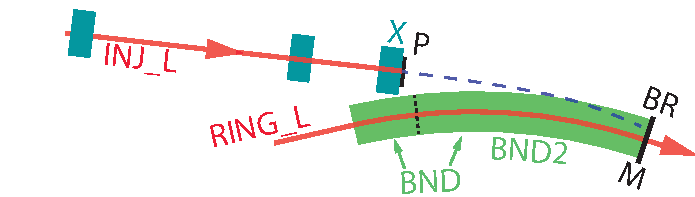
\includegraphics[width=5in]{injection.pdf}
  \caption[Injection line into a dipole magnet.]{
Injection line into a dipole magnet.
  }
  \label{f:inject}
\end{figure}

An injection line is illustrated in \fig{f:inject}. In this example,
The path of an injected particle after it leaves the last element
\vn{X} of the injection line (dashed blue line) partially goes through
the field of the dipole \vn{BND} in the storage ring. One way to
simulate this is:
\begin{example}
  INJ_L: line = (..., X, P, BND2, BR)
  RING_L: line = (..., BND, M, ...)
  P: patch, x_offset = -0.5, x_pitch = 0.15, z_offset = 0.3 
  BND: sbend, l = 6.2, g = 1/52
  BND2: BND, l = 4.7, tracking_method = runge_kutta,
          field_calc = fieldmap, grid_field = \{...\}
  BR: fork, to_line = RING_L, to_element = M
  M: marker
  use, INJ_L
\end{example}

In order to properly track particles through the fringe field of the
dipole \vn{BND}, a partial section of \vn{BND}, called \vn{BND2}, is
placed in the injection line \vn{INJ_L}. The \vn{tracking_method} for
\vn{BND2} is set to \vn{runge_kutta} since the default
\vn{bmad_standard} tracking is not able to handle these fringe
fields. Additionally, the \vn{field_calc} parameter of \vn{BND2} is
set to \vn{field map} so that the actual field profile of this particular
magnet can be used in the tracking. The field is specified in the
\vn{grid_field} parameter (\sref{s:fieldmap}). 

After traversing element \vn{X} in the injection line, the particle
goes through the patch \vn{P} which offsets the reference trajectory
so that following element, \vn{BND2}, is properly positioned.  The
beginning of \vn{BND2} is marked by a black dashed line in the figure.
At the end of \vn{BND2} the fork element \vn{BR} connects \vn{INJ_L}
with the marker \vn{M} in \vn{RING_L}.

%-----------------------------------------------------------------------------
\section{Example: Energy Recovery Linac}
\label{s:ex.erl}

\begin{figure}[tb]
  \centering
  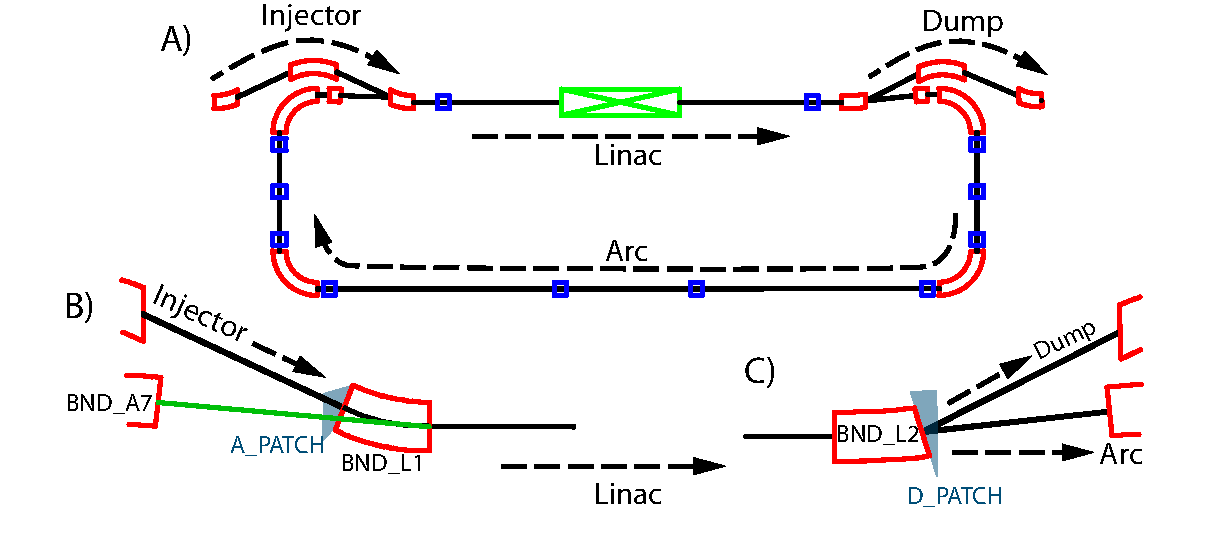
\includegraphics[width=6in]{erl.pdf}
  \caption[Example Energy Recovery Linac.]{
Example Energy Recovery Linac. A) The ERL consists of an injection
line, accelerating linac, return arc, decellerating linac, and finally
a beam dump. B) Close up of the section where the end of the injector
and the end of the arc inject into the beginning of the linac. C)
Close up of the end of the linac which injects into the dump and the
beginning of the arc.}
  \label{f:erl}
\end{figure}

An Energy Recovery Linac (ERL) is illustrated in \fig{f:erl}A. The ERL
starts with an injection line that feeds a linac which accelerates the
beam to some energy. The beam then transverses a return \vn{arc} which
reinjects the bunches into the linac. The length of the return arc is
such that, on the second pass, the beam is decelleratied giving its
energy back to the RF cavities. Finally, the decelleratied beam is
steered through a dump line where, at the end, an absorber stops the
beam.

 A lattice file for modeling this ERL:
\begin{example}
  parameter[geometry] = open
  parameter[absolute_time_tracking] = T

  BEND_L1: sbend, angle = -25*pi/180, l = 0.2, ...
  BEND_L2: BEND_L1

  A_PATCH: patch, flexible = T
  D_PATCH: patch, x_offset = 0.034, x_ptich = asin(0.32) 
  INJECT: line = (...)
  LINAC: line[multipass] = (BEND_L1, ..., BEND_L2)
  ARC: line = (..., BEND_A7)
  DUMP: line = (...)

  ERL: line = (INJECT, LINAC, ARC, A_PATCH, LINAC, D_PATCH, DUMP)
\end{example}

\index{patch!example}
\fig{f:erl}B shows the injector and arc merging into the beginning of
the linac. The first element of the linac is a bend named
\vn{BEND_L1}. The bending angle for \vn{BEND_L1} has been set at the
appropriate value for injection from the injector. To get the correct
geometry for injection from the arc, a \vn{patch} element, named
\vn{A_PATCH}, is placed in the \vn{ERL} line between the arc and the
linac. \vn{A_PATCH} is a flexible patch which means that the exit edge
of \vn{A_PATCH} will automatically be aligned with the entrance edge
of the next element which is \vn{BEND_L1}. 

Note that this use of a flexible patch works since the orientation of
\vn{BEND_L1} has been determined before the orientaiton of
\vn{A_PATCH} is determined. The orientaiton of elements is determined
in order starting from the first element in the line (the exception to
this rule is if there is a \vn{floor_position} element) and the
orientation of \vn{BEND_L1} is thus determined right after the
injector section on the first pass through the linac.



\fig{f:erl}C shows the end of the linac splitting off into the dump
and arc sections. The l

A patch
element named \vn{A_PATCH} is used

%-----------------------------------------------------------------------------
\section{Example: Patch Between reversed and non-reversed elements}
\label{s:ex.patch}

\begin{figure}[tb]
  \centering
  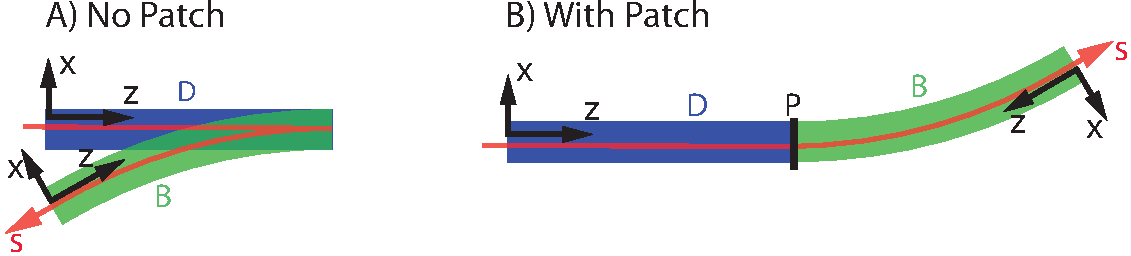
\includegraphics[width=5in]{patch-between.pdf}
  \caption[Patching between reversed and non-reversed elements.]{
Drift element \vn{D} is followed by a reversed drift element \vn{B}.
The view is from $+y$ onto the $x$-$z$ plane. A) If no patch is
present then the geometry does not make physical sense. B) With a
patch in between, a sane geometry can be obtained.}
  \label{f:patch.between}
\end{figure}

\index{patch}
Between normal and reversed elements there must be a reflection
\vn{patch} element (\sref{s:patch}).  This is illustrated in
\fig{f:patch.between}. The basic lattice is
\begin{example}
  D: drift, l = 2
  g_design = pi/12
  B: sbend, l = 2, g = g_design, g_err = -2*g_design
  P: patch, x_pitch = pi
  A_line: line = (D, --B)     ! Illegal. Do not use!
  B_line: line = (D, P, --B)  ! Correct
\end{example}
Line \vn{A_line} represents the situation shown in
\fig{f:patch.between}A.  With no patch between the drift \vn{D} and
the reversed bend \vn{B}, a particle leaving \vn{D} at \vn{D}'s
downstream end will find itself outside of both \vn{D} and
\vn{B}. Clearly this is an unphysical situation. Sanity is restored in
line \vn{B_line} shown in \fig{f:patch.between}B. In this instance, the
patch \vn{P} rotates the reference coordinates around the $y$-axis
leaving the $y$-axis invariant the bend of \vn{B} is in the $x$-$z$
plane. There are other patch parameter values that could be used to
produce a reflection patch (\sref{s:reflect.patch}).  For example,
Setting the patch's \vn{y_pitch} to \vn{pi} would produce a reflection
patch.

Since bend \vn{B} is reversed, A particle moving downstream within
\vn{B} is going the opposite direction from the normal direction. If
\vn{g_err} were zero in this instance, a downstream moving particle
would feel a force that will rotate the particle in a clockwise manner
opposite from the counterclockwise direction of the bend. To counter
this, \vn{g_err} is set so the total bending field \vn{g_tot = g +
g_err} is opposite the design field. That is, \vn{g_err} is set so
that \vn{g_tot = -g}.

%-----------------------------------------------------------------------------
\section{Example: Colliding Beam Storage Rings}
\label{s:ex.collide}

\begin{figure}[tb]
  \centering
  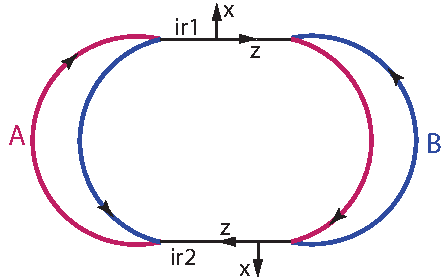
\includegraphics[width=5in]{colliding-beams.pdf}
  \caption[Dual ring colliding beam machine]{Dual ring colliding beam machine. 
The beam in the \vn{A} ring rotates clockwise and in the \vn{B} ring
counterclockwise.}
  \label{f:collide}
\end{figure}

The idealized layout of a pair of storage rings used for colliding
counter rotating beams is shown in \fig{f:collide}. Rings \vn{A} and
\vn{B} intersect at two interaction regions labeled \vn{ir1} and
\vn{ir2} where the beams collide. The basic lattice description is:
\begin{example}
  ir1: line[multipass] = (...)
  ir2: line[multipass] = (...)
  pa1_in; patch, ...
  pa1_out; patch, ...
  pa2_in; patch, ...
  pa2_out; patch, ...
  m: marker
  fid: fiducial, origin_ele = m
  ...
  A: line = (arc_a1, pa1_in, ir1, m, pa1_out, arc_a2, pa2_in, ir2, pa2_out)
  B_rev: line = (arc_b1, pb1_in, ir1, fid, pb1_out, arc_b2, pb2_in, ir2, pb2_out)
  B: line = (--B_rev)
  use, A, B
\end{example}
Lines \vn{ir1} and \vn{ir2} are the two interaction regions which are
declared \vn{multipass} since they are shared by the two rings. Line
\vn{A} represents ring \vn{A} where the beam which, by definition,
travels in the same direction as increasing $s$, rotates clockwise.
Line \vn{B_rev} is a ``reversed'' line of ring \vn{B} and, like
\vn{a}, represents a beam rotating clockwise.  Line \vn{B}, which
represents ring \vn{B}, is the reverse of \vn{B_rev} and here the beam
rotates counterclockwise. In this construction, all elements of \vn{B}
are reversed.  While this is not mandatory (only the interaction
regions must be reversed in \vn{B}), having all of \vn{B} reversed
simplifies the geometry since this Means that the local coordinate
systems of both lines \vn{A} and \vn{b} will be ``aligned'' with the
$x$-axis pointing to the outside of the ring and the $y$-axis pointing
up, out of the page. Having non-aligned coordinate systems is possible
but potentially very confusing.

The two rings are physically aligned using a marker \vn{m} in \vn{A}
and a \vn{fiducial} element \vn{fid} in \vn{B} that aligns with
\vn{m}.  Each ring has four rigid \vn{patch} elements, whose name
begins with \vn{p}, on either side of each interaction region.

The finished lattice will have two branches, The first branch (with
index 0) will be derived from line \vn{a} (and hence will be named
``a'') and the second branch (with index 1) will be derived from line
\vn{b} (and hence will be named ``b''). The multipass lords
representing the physical IR elements will be in the ``lord section''
of branch 0.


%-----------------------------------------------------------------------------
\subsection{Example: Backward Tracking Through a Lattice}
\label{s:reverse}

By creating a reversed lattice, one can essentially track particles backwards. For example,
assume that you have a lattice file called \vn{original_lattice.bmad} which defines a line
called \vn{original_line}. To create a reversed lattice, create a new file with the following:
\begin{example}
  call, file = orginal_lattice.bmad
  reversed_line: line = (--original_line)
  parameter[particle] = antiparticle(parameter[particle])
  use, reversed_line
\end{example}
The ``\vn{--}'' reverses the line and reverses the elements (\sref{s:ele.reverse}). Tracking through
\vn{reversed_line} is equivalent to tracking backwards through \vn{orginal_line}.  

If the \vn{original_line} lattice had just static magnetic fields and no electric fields, then
by tracking with the anti-particle in the reversed lattice, the anti-particle will follow the same
path (but backward) as the the particle in the original lattice. For this to work, the anti-particle
must be started with the appropriate phase space coordinates. If $(x, p_x, y, p_y, z, p_z)$ is
the phase space coordinates of the particle at the end of the original lattice, the anti-particle
must be initialized with phase space coordinates of $(x, -p_x, y, -p_y, \text{immaterial}, p_z)$.

\chapter{MAD/XSIF/SAD/PTC Lattice Conversion}
\label{c:lat.convert}
\index{conversion to other lattice formats}

%-----------------------------------------------------------------------------
\section{MAD Conversion}
\label{s:mad.convert}
\index{MAD!conversion}

%-----------------------------------------------------------------------------
\subsection{Convert MAD to Bmad Via UAP}
\label{s:mad.bmad.uap}

Conversion of lattice files from \mad to \bmad format can be done using the \vn{Universal
Accelerator Parser} (\sref{s:aml}). 
Due to differences in language definitions, the conversions must be done with some
care. The following differences should be noted:
  \begin{itemize}
  \item
\bmad, unlike \mad, does not have any ``action'' commands. An action
command is a command that makes a calculation. Examples include \mad's
\vn{SURVEY} and \vn{TWISS} commands.
  \item
In \bmad all variables must be defined. In \mad undefined variables
will default to 0.
  \item
In \bmad all variables must be defined before being used
(\sref{s:arith}) while \mad does not have this constraint.
  \item
\bmad, unlike \mad, does not allow variable values to be redefined.
  \item
Elements like a \vn{sad_mult} cannot be translated.
  \end{itemize}

%-----------------------------------------------------------------------------
\subsection{Convert Bmad to MAD}
\label{s:bmad.mad}

\index{wiggler!conversion to MAD}
\index{sol_quad!conversion to MAD}
Besides using the \vn{Universal Accelerator Parser} for conversion
from \bmad to \mad, there is a \bmad conversion routine called
\Hyperref{r:write.lattice.in.foreign.format}{write_lattice_in_foreign_format}. 
The advantage of this routine is that since \mad does not have a
\vn{wiggler} or a \vn{sol_quad} element, this conversion routine can
make an ``equivalent'' substitution. For a \vn{sol_quad}, the
equivalent substitution will be a drift-matrix-drift series of
elements. For a \vn{wiggler}, a series of bend and drift elements will
be used (the program can also use a drift-matrix-drift model here but
that is not as accurate). The bends and drifts for the \vn{wiggler}
model are constructed so that the global geometry of the lattice does
not change. Additionally the bends and drifts are constructed to most
nearly match the wiggler's
\begin{example}
  Transfer matrix
  $I_2$ and $I_3$ synchrotron radiation integrals (\sref{s:synch.ints})
\end{example}
Note that the resulting model will not have the vertical cubic
nonlinearity that the actual wiggler has.

The \vn{bmad_to_mad_or_xsif} routine is embeded in the program
\vn{util_programs/bmad_to_mad_or_xsif}.

%-----------------------------------------------------------------------------
%\subsection{Convert MAD-X to Bmad Via PTC}
%\label{s:mad.bmad.ptc}
%
%\mad-X lattices can be converted to \bmad by first using \mad-X to create a PTC ``flat''
%file and then using \bmad to convert the flat file to a \bmad lattice file. 
%
%The advantage of converting via PTC rather than using UAP (\sref{s:mad.bmad.uap}) is that
%one does not have to worry about removing action commands from the \mad-X file. The
%disadvantages are:
%  \begin{description}
%  \item 
%the conversion does not preserve any of the look and feel of the original \mad-X file. 
%  \item
%the conversion via PTC does not work with \mad8 lattices.
%  \item
%\mad-X does not correctly handle \vn{elseparator} and \vn{matrix} elements. These
%elements become drifts in a flat file.
%  \item
%\mad-X does not transfer beginning Twiss and orbit information to the flat file needed for open lattices.
%  \item
%\mad-X does not transfer the zeroth (dipole) order multipoles of a multipole element to the flat file.
%  \end{description}
%
%First, take a \mad-X lattice file and append the following to it:
%\begin{example}
%  use, period = LINE_NAME_HERE;
%  ptc_create_universe;
%  ptc_create_layout, model = 1, method = 2, nst = 1; 
%  !! ptc_create_layout, model=1, method=2, nst=1, exact;  ! Use this if exact is wanted
%  ptc_script, file="create_flat.ptc";
%\end{example}
%Substitute the actual sequence or line name for ``LINE_NAME_HERE''.
%
%Second, create a file called \vn{create_flat.ptc} with the following in it:
%\begin{example}
%  select layout
%  1
%  print flat file
%  XXX.flat
%  return
%\end{example}
%The flat file name \vn{XXX.flat} can be changed if desired.
%
%Now run \mad-X with the lattice file. A flat file will be created. This flat file can
%converted to \bmad as documented in \sref{s:ptc.convert}

%---------------------------------------------------------------------------
\section{XSIF Conversion}
\label{s:xsif.convert}
\index{XSIF!conversion}

XSIF\cite{b:xsif}, developed at SLAC, stands for ``Extended Standard
Input Format.''  XSIF is essentially a subset of the
\mad\cite{b:maduser} input format.

\bmad has software to directly parse XSIF files so XSIF files may be
used in place of \bmad lattice files.  With some restrictions, an XSIF
lattice file may be called from within a \bmad lattice file. See
Section~\sref{s:call} for details.

\index{parameter statement!geometry}
Since XSIF does not have a \vn{parameter[geometry]} statement
(\sref{s:param}), the type of the lattice (whether circular or linear)
is determined by the presence or absence of any \vn{lcavity} elements
in the XSIF file. This is independent of whether \vn{lcavity} elements
are actually used in the lattice.

Note: One point that is not covered in the XSIF documentation is that
for a \vn{MATRIX} element, unlike \mad, the \vn{R$ii$} terms (the
diagonal terms of the linear matrix) are not unity by default. Thus
\index{MAD}
\begin{example}
  m: matrix
\end{example}
in an XSIF file will give a matrix with all elements being zero.

To convert between XSIF and \bmad the \vn{Universal Accelerator
Parser} can be used (\sref{s:aml}). Additionally, the
\vn{bmad_to_mad_or_xsif} routine in \bmad can convert from \bmad to
XSIF (cf.~\sref{s:mad.convert}).

%---------------------------------------------------------------------------
%\section{PTC Conversion}
%\label{s:ptc.convert}
%\index{ptc!conversion}
%
%For a programmer, 
%For conversion from \bmad to PTC there are two possibilites

%---------------------------------------------------------------------------
\section{SAD Conversion}
\label{s:sad.convert}
\index{SAD}

Conversion from \vn{SAD}\cite{b:sad} to \bmad is accomplished using the Python script
\begin{example}
  util_programs/sad_to_bmad/sad_to_bmad.py
\end{example}
Currently, a converter from \bmad to SAD is planned but has not been implemented.

Currently, the following restrictions on SAD lattices apply:
  \begin{itemize}
  \item
SAD must elements cannot have an associated RF field
  \item
Misalignments in a \vn{sol} element with \vn{geo} = 1 cannot be handled.
  \end{itemize}

%----------------------------------------------------------------------------
\section{Translation Using the Universal Accelerator Parser}
\label{s:aml}
\index{Accelerator Markup Language (AML)}
\index{Universal Accelerator Parser (UAP)}

\index{MAD}
The \vn{Accelerator Markup Language} (\vn{AML}) / \vn{Universal
Accelerator Parser} (\vn{UAP}) project\cite{b:aml} is a collaborative
effort with the aim of 1) creating a lattice format (the \vn{AML}
part) that can be used to fully describe accelerators and storage
rings, and 2) producing software (the \vn{UAP} part) that can parse
\vn{AML} lattice files. A side benefit of this project is that the
\vn{UAP} code has been extended to be able to translate between
\vn{AML}, \bmad, \mad-8, \mad-X, and \vn{XSIF}. 

The program
\vn{translate_driver} which comes with the \vn{UAP} code can be used
for conversions. To get help with how to run this program use the command
\begin{example}
  path-to-uap-dir/bin/translate_driver -help
\end{example}
Example:
\begin{example}
  path-to-uap-dir/bin/translate_driver -constants_first -bmad xxx.madx
\end{example}
This will convert a \mad-X file \vn{xxx.madx} to \bmad format.

\chapter{List of Element Attributes}
\label{c:attrib.list}

Alphabetical list of element attributes for each type of element. 

Note for programmers: The program that generates a file of attributes indexed by the
internal reference number is:
\begin{example}
  util_programs/element_attributes.f90 
\end{example}

 %---------------------------------
 \section{AB_multipole Element Element Attributes}
 \label{s:list.ab.multipole}
 
 \begin{tabular}{llll} \toprule
a0 - a20, b0 - b20          & field_master                & ref_origin                  & x_limit                     \\
alias                       & is_on                       & spin_tracking_method        & x_offset                    \\
aperture                    & l                           & superimpose                 & x_offset_tot                \\
aperture_at                 & mat6_calc_method            & tilt                        & y1_limit                    \\
aperture_type               & multipoles_on               & tilt_tot                    & y2_limit                    \\
create_jumbo_slave          & offset                      & tracking_method             & y_limit                     \\
delta_ref_time              & offset_moves_aperture       & type                        & y_offset                    \\
descrip                     & p0c                         & wall                        & y_offset_tot                \\
ele_origin                  & ptc_integration_type        & x1_limit                    & z_offset                    \\
e_tot                       & reference                   & x2_limit                    & z_offset_tot                \\
 \bottomrule
 \end{tabular}
 \vfill
 
 %---------------------------------
 \section{AC_Kicker Element Element Attributes}
 \label{s:list.ac.kicker}
 
 \begin{tabular}{llll} \toprule
a0 - a20, b0 - b20          & frequencies                 & offset_moves_aperture       & vkick                       \\
alias                       & fringe_at                   & p0c                         & wall                        \\
amp_vs_time                 & fringe_type                 & ptc_integration_type        & x1_limit                    \\
aperture                    & grid_field                  & r0_elec                     & x2_limit                    \\
aperture_at                 & hkick                       & r0_mag                      & x_limit                     \\
aperture_type               & integrator_order            & reference                   & x_offset                    \\
bl_hkick                    & is_on                       & ref_origin                  & x_offset_tot                \\
bl_vkick                    & l                           & scale_multipoles            & x_pitch                     \\
cartesian_map               & lord_pad1                   & spin_fringe_on              & x_pitch_tot                 \\
create_jumbo_slave          & lord_pad2                   & spin_tracking_method        & y1_limit                    \\
csr_calc_on                 & lr_freq_spread              & sr_wake_file                & y2_limit                    \\
cylindrical_map             & lr_self_wake_on             & superimpose                 & y_limit                     \\
delta_ref_time              & lr_wake_file                & symplectify                 & y_offset                    \\
descrip                     & lr_wake_spline              & taylor_field                & y_offset_tot                \\
ds_step                     & l_hard_edge                 & taylor_map_includes_offsets & y_pitch                     \\
ele_origin                  & mat6_calc_method            & tilt                        & y_pitch_tot                 \\
e_tot                       & multipoles_on               & tilt_tot                    & z_offset                    \\
field_calc                  & num_steps                   & tracking_method             & z_offset_tot                \\
field_master                & n_ref_pass                  & type                        &                             \\
field_overlaps              & offset                      & t_offset                    &                             \\
 \bottomrule
 \end{tabular}
 \vfill
 
 %---------------------------------
 \section{BeamBeam Element Element Attributes}
 \label{s:list.beambeam}
 
 \begin{tabular}{llll} \toprule
alias                       & delta_ref_time              & ref_origin                  & x_offset_tot                \\
alpha_a                     & descrip                     & sig_x                       & x_pitch                     \\
alpha_b                     & ele_origin                  & sig_y                       & x_pitch_tot                 \\
aperture                    & e_tot                       & sig_z                       & y1_limit                    \\
aperture_at                 & field_calc                  & spin_tracking_method        & y2_limit                    \\
aperture_type               & is_on                       & superimpose                 & y_limit                     \\
bbi_constant                & l                           & tilt                        & y_offset                    \\
beta_a                      & mat6_calc_method            & tilt_tot                    & y_offset_tot                \\
beta_b                      & n_slice                     & tracking_method             & y_pitch                     \\
charge                      & n_slice                     & type                        & y_pitch_tot                 \\
cmat_11                     & offset                      & wall                        & z_offset                    \\
cmat_12                     & offset_moves_aperture       & x1_limit                    & z_offset_tot                \\
cmat_21                     & p0c                         & x2_limit                    &                             \\
cmat_22                     & ptc_integration_type        & x_limit                     &                             \\
create_jumbo_slave          & reference                   & x_offset                    &                             \\
 \bottomrule
 \end{tabular}
 \vfill
 
 %---------------------------------
 \section{Bend_Sol_Quad Element Element Attributes}
 \label{s:list.bend.sol.quad}
 
 \begin{tabular}{llll} \toprule
a0 - a20, b0 - b20          & field_master                & offset                      & vkick                       \\
alias                       & field_overlaps              & offset_moves_aperture       & wall                        \\
angle                       & fringe_at                   & p0c                         & x1_limit                    \\
aperture                    & fringe_type                 & ptc_canonical_coords        & x2_limit                    \\
aperture_at                 & g                           & ptc_integration_type        & x_limit                     \\
aperture_type               & grid_field                  & quad_tilt                   & x_offset                    \\
b1_gradient                 & hkick                       & r0_elec                     & x_offset_tot                \\
bend_tilt                   & integrator_order            & r0_mag                      & x_pitch                     \\
bl_hkick                    & is_on                       & reference                   & x_pitch_tot                 \\
bl_vkick                    & k1                          & ref_origin                  & x_quad                      \\
bs_field                    & ks                          & rho                         & y1_limit                    \\
b_field                     & l                           & scale_multipoles            & y2_limit                    \\
cartesian_map               & lord_pad1                   & spin_fringe_on              & y_limit                     \\
create_jumbo_slave          & lord_pad2                   & spin_tracking_method        & y_offset                    \\
csr_calc_on                 & lr_freq_spread              & sr_wake_file                & y_offset_tot                \\
cylindrical_map             & lr_self_wake_on             & superimpose                 & y_pitch                     \\
delta_ref_time              & lr_wake_file                & symplectify                 & y_pitch_tot                 \\
descrip                     & lr_wake_spline              & taylor_field                & y_quad                      \\
dks_ds                      & l_hard_edge                 & taylor_map_includes_offsets & z_offset                    \\
ds_step                     & mat6_calc_method            & tilt                        & z_offset_tot                \\
ele_origin                  & multipoles_on               & tilt_tot                    &                             \\
e_tot                       & num_steps                   & tracking_method             &                             \\
field_calc                  & n_ref_pass                  & type                        &                             \\
 \bottomrule
 \end{tabular}
 \vfill
 
 %---------------------------------
 \section{Capillary Element Element Attributes}
 \label{s:list.capillary}
 
 \begin{tabular}{llll} \toprule
alias                       & mat6_calc_method            & tilt                        & x_pitch_tot                 \\
aperture                    & n_slice_spline              & tilt_tot                    & y1_limit                    \\
aperture_at                 & offset                      & tracking_method             & y2_limit                    \\
aperture_type               & offset_moves_aperture       & type                        & y_limit                     \\
create_jumbo_slave          & p0c                         & wall                        & y_offset                    \\
critical_angle_factor       & ptc_integration_type        & x1_limit                    & y_offset_tot                \\
delta_ref_time              & reference                   & x2_limit                    & y_pitch                     \\
descrip                     & ref_origin                  & x_limit                     & y_pitch_tot                 \\
ele_origin                  & spin_tracking_method        & x_offset                    & z_offset                    \\
e_tot                       & superimpose                 & x_offset_tot                & z_offset_tot                \\
l                           & s_spline                    & x_pitch                     &                             \\
 \bottomrule
 \end{tabular}
 \vfill
 
 %---------------------------------
 \section{Crystal Element Element Attributes}
 \label{s:list.crystal}
 
 \begin{tabular}{llll} \toprule
alias                       & descrip                     & ref_orbit_follows           & x1_limit                    \\
alpha_angle                 & diffraction_limited         & ref_origin                  & x2_limit                    \\
aperture                    & d_spacing                   & ref_tilt                    & x_limit                     \\
aperture_at                 & ele_origin                  & ref_tilt_tot                & x_offset                    \\
aperture_type               & e_tot                       & ref_wavelength              & x_offset_tot                \\
bragg_angle                 & l                           & spin_tracking_method        & x_pitch                     \\
bragg_angle_in              & mat6_calc_method            & superimpose                 & x_pitch_tot                 \\
bragg_angle_out             & offset                      & surface                     & y1_limit                    \\
b_param                     & offset_moves_aperture       & thickness                   & y2_limit                    \\
create_jumbo_slave          & p0c                         & tilt                        & y_limit                     \\
crystal_type                & pendellosung_period_pi      & tilt_corr                   & y_offset                    \\
curvature_x0_y2             & pendellosung_period_sigma   & tilt_tot                    & y_offset_tot                \\
darwin_width_pi             & psi_angle                   & tracking_method             & y_pitch                     \\
darwin_width_sigma          & ptc_integration_type        & type                        & y_pitch_tot                 \\
dbragg_angle_de             & reference                   & v_unitcell                  & z_offset                    \\
delta_ref_time              & ref_cap_gamma               & wall                        & z_offset_tot                \\
 \bottomrule
 \end{tabular}
 \vfill
 
 %---------------------------------
 \section{Custom Element Element Attributes}
 \label{s:list.custom}
 
 \begin{tabular}{llll} \toprule
alias                       & lord_pad1                   & superimpose                 & wall                        \\
aperture                    & lord_pad2                   & symplectify                 & x1_limit                    \\
aperture_at                 & lr_freq_spread              & taylor_map_includes_offsets & x2_limit                    \\
aperture_type               & lr_self_wake_on             & tilt                        & x_limit                     \\
create_jumbo_slave          & lr_wake_file                & tilt_tot                    & x_offset                    \\
csr_calc_on                 & lr_wake_spline              & tracking_method             & x_offset_tot                \\
delta_e                     & l_hard_edge                 & type                        & x_pitch                     \\
delta_ref_time              & mat6_calc_method            & val1                        & x_pitch_tot                 \\
descrip                     & num_steps                   & val10                       & y1_limit                    \\
ds_step                     & n_ref_pass                  & val11                       & y2_limit                    \\
ele_origin                  & offset                      & val12                       & y_limit                     \\
e_tot                       & offset_moves_aperture       & val2                        & y_offset                    \\
e_tot_start                 & p0c                         & val3                        & y_offset_tot                \\
field_calc                  & p0c_start                   & val4                        & y_pitch                     \\
field_master                & ptc_integration_type        & val5                        & y_pitch_tot                 \\
field_overlaps              & reference                   & val6                        & z_offset                    \\
integrator_order            & ref_origin                  & val7                        & z_offset_tot                \\
is_on                       & spin_tracking_method        & val8                        &                             \\
l                           & sr_wake_file                & val9                        &                             \\
 \bottomrule
 \end{tabular}
 \vfill
 
 %---------------------------------
 \section{Detector Element Element Attributes}
 \label{s:list.detector}
 
 \begin{tabular}{llll} \toprule
alias                       & l                           & tilt                        & x_pitch                     \\
aperture                    & mat6_calc_method            & tilt_calib                  & x_pitch_tot                 \\
aperture_at                 & noise                       & tilt_tot                    & y1_limit                    \\
aperture_type               & n_sample                    & tracking_method             & y2_limit                    \\
create_jumbo_slave          & offset                      & type                        & y_gain_calib                \\
crunch                      & offset_moves_aperture       & wall                        & y_gain_err                  \\
crunch_calib                & osc_amplitude               & x1_limit                    & y_limit                     \\
curvature_x0_y2             & p0c                         & x2_limit                    & y_offset                    \\
delta_ref_time              & ptc_integration_type        & x_gain_calib                & y_offset_calib              \\
descrip                     & reference                   & x_gain_err                  & y_offset_tot                \\
de_eta_meas                 & ref_origin                  & x_limit                     & y_pitch                     \\
ele_origin                  & spin_tracking_method        & x_offset                    & y_pitch_tot                 \\
e_tot                       & superimpose                 & x_offset_calib              & z_offset                    \\
is_on                       & surface                     & x_offset_tot                & z_offset_tot                \\
 \bottomrule
 \end{tabular}
 \vfill
 
 %---------------------------------
 \section{Diffraction_Plate Element Element Attributes}
 \label{s:list.diffraction.plate}
 
 \begin{tabular}{llll} \toprule
alias                       & mat6_calc_method            & tilt                        & y1_limit                    \\
aperture                    & mode                        & tilt_tot                    & y2_limit                    \\
aperture_at                 & offset                      & tracking_method             & y_limit                     \\
aperture_type               & offset_moves_aperture       & type                        & y_offset                    \\
create_jumbo_slave          & p0c                         & wall                        & y_offset_tot                \\
curvature_x0_y2             & ptc_integration_type        & x1_limit                    & y_pitch                     \\
delta_ref_time              & reference                   & x2_limit                    & y_pitch_tot                 \\
descrip                     & ref_origin                  & x_limit                     & z_offset                    \\
ele_origin                  & ref_wavelength              & x_offset                    & z_offset_tot                \\
e_tot                       & spin_tracking_method        & x_offset_tot                &                             \\
field_scale_factor          & superimpose                 & x_pitch                     &                             \\
is_on                       & surface                     & x_pitch_tot                 &                             \\
 \bottomrule
 \end{tabular}
 \vfill
 
 %---------------------------------
 \section{Drift Element Element Attributes}
 \label{s:list.drift}
 
 \begin{tabular}{llll} \toprule
alias                       & l                           & superimpose                 & x_pitch                     \\
aperture                    & lord_pad1                   & symplectify                 & x_pitch_tot                 \\
aperture_at                 & lord_pad2                   & taylor_map_includes_offsets & y1_limit                    \\
aperture_type               & mat6_calc_method            & tilt                        & y2_limit                    \\
create_jumbo_slave          & num_steps                   & tilt_tot                    & y_limit                     \\
csr_calc_on                 & n_ref_pass                  & tracking_method             & y_offset                    \\
delta_ref_time              & offset                      & type                        & y_offset_tot                \\
descrip                     & offset_moves_aperture       & wall                        & y_pitch                     \\
ds_step                     & p0c                         & x1_limit                    & y_pitch_tot                 \\
ele_origin                  & ptc_integration_type        & x2_limit                    & z_offset                    \\
e_tot                       & reference                   & x_limit                     & z_offset_tot                \\
field_calc                  & ref_origin                  & x_offset                    &                             \\
integrator_order            & spin_tracking_method        & x_offset_tot                &                             \\
 \bottomrule
 \end{tabular}
 \vfill
 
 %---------------------------------
 \section{ELseparator Element Element Attributes}
 \label{s:list.elseparator}
 
 \begin{tabular}{llll} \toprule
a0 - a20, b0 - b20          & gap                         & ptc_canonical_coords        & wall                        \\
alias                       & grid_field                  & ptc_integration_type        & x1_limit                    \\
aperture                    & hkick                       & r0_elec                     & x2_limit                    \\
aperture_at                 & integrator_order            & r0_mag                      & x_limit                     \\
aperture_type               & is_on                       & reference                   & x_offset                    \\
cartesian_map               & l                           & ref_origin                  & x_offset_tot                \\
create_jumbo_slave          & lord_pad1                   & scale_multipoles            & x_pitch                     \\
csr_calc_on                 & lord_pad2                   & spin_fringe_on              & x_pitch_tot                 \\
cylindrical_map             & lr_freq_spread              & spin_tracking_method        & y1_limit                    \\
delta_ref_time              & lr_self_wake_on             & sr_wake_file                & y2_limit                    \\
descrip                     & lr_wake_file                & superimpose                 & y_limit                     \\
ds_step                     & lr_wake_spline              & symplectify                 & y_offset                    \\
ele_origin                  & l_hard_edge                 & taylor_field                & y_offset_tot                \\
e_field                     & mat6_calc_method            & taylor_map_includes_offsets & y_pitch                     \\
e_tot                       & multipoles_on               & tilt                        & y_pitch_tot                 \\
field_calc                  & num_steps                   & tilt_tot                    & z_offset                    \\
field_master                & n_ref_pass                  & tracking_method             & z_offset_tot                \\
field_overlaps              & offset                      & type                        &                             \\
fringe_at                   & offset_moves_aperture       & vkick                       &                             \\
fringe_type                 & p0c                         & voltage                     &                             \\
 \bottomrule
 \end{tabular}
 \vfill
 
 %---------------------------------
 \section{EM_Field Element Element Attributes}
 \label{s:list.em.field}
 
 \begin{tabular}{llll} \toprule
alias                       & field_overlaps              & p0c                         & tracking_method             \\
aperture                    & fringe_at                   & p0c_start                   & type                        \\
aperture_at                 & fringe_type                 & phi0                        & wall                        \\
aperture_type               & grid_field                  & phi0_autoscale              & x1_limit                    \\
autoscale_amplitude         & integrator_order            & phi0_err                    & x2_limit                    \\
autoscale_phase             & is_on                       & ptc_canonical_coords        & x_limit                     \\
cartesian_map               & l                           & ptc_integration_type        & x_offset                    \\
constant_ref_energy         & lord_pad1                   & reference                   & x_offset_tot                \\
create_jumbo_slave          & lord_pad2                   & ref_origin                  & x_pitch                     \\
csr_calc_on                 & lr_freq_spread              & rf_frequency                & x_pitch_tot                 \\
cylindrical_map             & lr_self_wake_on             & spin_fringe_on              & y1_limit                    \\
delta_ref_time              & lr_wake_file                & spin_tracking_method        & y2_limit                    \\
descrip                     & lr_wake_spline              & sr_wake_file                & y_limit                     \\
ds_step                     & l_hard_edge                 & superimpose                 & y_offset                    \\
ele_origin                  & mat6_calc_method            & symplectify                 & y_offset_tot                \\
e_tot                       & num_steps                   & taylor_field                & y_pitch                     \\
e_tot_start                 & n_ref_pass                  & taylor_map_includes_offsets & y_pitch_tot                 \\
field_autoscale             & offset                      & tilt                        & z_offset                    \\
field_calc                  & offset_moves_aperture       & tilt_tot                    & z_offset_tot                \\
 \bottomrule
 \end{tabular}
 \vfill
 
 %---------------------------------
 \section{E_Gun Element Element Attributes}
 \label{s:list.e.gun}
 
 \begin{tabular}{llll} \toprule
alias                       & fringe_type                 & p0c                         & voltage                     \\
aperture                    & gradient                    & phi0                        & voltage_err                 \\
aperture_at                 & gradient_err                & phi0_autoscale              & wall                        \\
aperture_type               & grid_field                  & phi0_err                    & x1_limit                    \\
autoscale_amplitude         & integrator_order            & ptc_integration_type        & x2_limit                    \\
autoscale_phase             & is_on                       & reference                   & x_limit                     \\
cartesian_map               & l                           & ref_origin                  & x_offset                    \\
create_jumbo_slave          & lord_pad1                   & rf_frequency                & x_offset_tot                \\
csr_calc_on                 & lord_pad2                   & spin_fringe_on              & x_pitch                     \\
cylindrical_map             & lr_freq_spread              & spin_tracking_method        & x_pitch_tot                 \\
delta_ref_time              & lr_self_wake_on             & sr_wake_file                & y1_limit                    \\
descrip                     & lr_wake_file                & superimpose                 & y2_limit                    \\
ds_step                     & lr_wake_spline              & symplectify                 & y_limit                     \\
ele_origin                  & l_hard_edge                 & taylor_field                & y_offset                    \\
e_tot                       & mat6_calc_method            & taylor_map_includes_offsets & y_offset_tot                \\
field_autoscale             & num_steps                   & tilt                        & y_pitch                     \\
field_calc                  & n_ref_pass                  & tilt_tot                    & y_pitch_tot                 \\
field_overlaps              & offset                      & tracking_method             & z_offset                    \\
fringe_at                   & offset_moves_aperture       & type                        & z_offset_tot                \\
 \bottomrule
 \end{tabular}
 \vfill
 
 %---------------------------------
 \section{Collimators: Ecollimator and Rcollimator Element Attributes}
 \label{s:list.collimator}
 
 \begin{tabular}{llll} \toprule
alias                       & hkick                       & ptc_integration_type        & x_limit                     \\
aperture                    & integrator_order            & reference                   & x_offset                    \\
aperture_at                 & is_on                       & ref_origin                  & x_offset_tot                \\
aperture_type               & l                           & spin_fringe_on              & x_pitch                     \\
bl_hkick                    & lord_pad1                   & spin_tracking_method        & x_pitch_tot                 \\
bl_vkick                    & lord_pad2                   & sr_wake_file                & y1_limit                    \\
create_jumbo_slave          & lr_freq_spread              & superimpose                 & y2_limit                    \\
csr_calc_on                 & lr_self_wake_on             & symplectify                 & y_limit                     \\
delta_ref_time              & lr_wake_file                & taylor_map_includes_offsets & y_offset                    \\
descrip                     & lr_wake_spline              & tilt                        & y_offset_tot                \\
ds_step                     & l_hard_edge                 & tilt_tot                    & y_pitch                     \\
ele_origin                  & mat6_calc_method            & tracking_method             & y_pitch_tot                 \\
e_tot                       & num_steps                   & type                        & z_offset                    \\
field_calc                  & n_ref_pass                  & vkick                       & z_offset_tot                \\
field_overlaps              & offset                      & wall                        &                             \\
fringe_at                   & offset_moves_aperture       & x1_limit                    &                             \\
fringe_type                 & p0c                         & x2_limit                    &                             \\
 \bottomrule
 \end{tabular}
 \vfill
 
 %---------------------------------
 \section{Fiducial Element Element Attributes}
 \label{s:list.fiducial}
 
 \begin{tabular}{llll} \toprule
alias                       & dx_origin                   & mat6_calc_method            & reference                   \\
delta_ref_time              & dy_origin                   & offset                      & ref_origin                  \\
descrip                     & dz_origin                   & origin_ele                  & spin_tracking_method        \\
dphi_origin                 & ele_origin                  & origin_ele_ref_pt           & superimpose                 \\
dpsi_origin                 & e_tot                       & p0c                         & tracking_method             \\
dtheta_origin               & l                           & ptc_integration_type        & type                        \\
 \bottomrule
 \end{tabular}
 \vfill
 
 %---------------------------------
 \section{Floor_Shift Element Element Attributes}
 \label{s:list.floor.shift}
 
 \begin{tabular}{llll} \toprule
alias                       & l                           & spin_tracking_method        & x_offset                    \\
aperture                    & mat6_calc_method            & superimpose                 & x_pitch                     \\
aperture_at                 & offset                      & tilt                        & y1_limit                    \\
aperture_type               & offset_moves_aperture       & tracking_method             & y2_limit                    \\
create_jumbo_slave          & origin_ele                  & type                        & y_limit                     \\
delta_ref_time              & origin_ele_ref_pt           & upstream_ele_dir            & y_offset                    \\
descrip                     & p0c                         & wall                        & y_pitch                     \\
downstream_ele_dir          & ptc_integration_type        & x1_limit                    & z_offset                    \\
ele_origin                  & reference                   & x2_limit                    &                             \\
e_tot                       & ref_origin                  & x_limit                     &                             \\
 \bottomrule
 \end{tabular}
 \vfill
 
 %---------------------------------
 \section{Fork and Photon_Fork Element Attributes}
 \label{s:list.fork}
 
 \begin{tabular}{llll} \toprule
alias                       & e_tot                       & p0c                         & type                        \\
aperture                    & is_on                       & ptc_integration_type        & x1_limit                    \\
aperture_at                 & ix_to_branch                & reference                   & x2_limit                    \\
aperture_type               & ix_to_element               & ref_origin                  & x_limit                     \\
create_jumbo_slave          & l                           & spin_tracking_method        & y1_limit                    \\
delta_ref_time              & mat6_calc_method            & superimpose                 & y2_limit                    \\
descrip                     & new_branch                  & to_element                  & y_limit                     \\
direction                   & offset                      & to_line                     &                             \\
ele_origin                  & offset_moves_aperture       & tracking_method             &                             \\
 \bottomrule
 \end{tabular}
 \vfill
 
 %---------------------------------
 \section{Girder Element Element Attributes}
 \label{s:list.girder}
 
 \begin{tabular}{llll} \toprule
alias                       & dz_origin                   & tilt                        & y_offset                    \\
descrip                     & is_on                       & tilt_tot                    & y_offset_tot                \\
dphi_origin                 & l                           & type                        & y_pitch                     \\
dpsi_origin                 & origin_ele                  & x_offset                    & y_pitch_tot                 \\
dtheta_origin               & origin_ele_ref_pt           & x_offset_tot                & z_offset                    \\
dx_origin                   & ref_tilt                    & x_pitch                     & z_offset_tot                \\
dy_origin                   & ref_tilt_tot                & x_pitch_tot                 &                             \\
 \bottomrule
 \end{tabular}
 \vfill
 
 %---------------------------------
 \section{Group Element Element Attributes}
 \label{s:list.group}
 
 \begin{tabular}{llll} \toprule
accordion_edge              & end_edge                    & s_position                  &                             \\
alias                       & gang                        & type                        &                             \\
descrip                     & start_edge                  & var                         &                             \\
 \bottomrule
 \end{tabular}
 \vfill
 
 %---------------------------------
 \section{Kickers: Hkicker and Vkicker Element Attributes}
 \label{s:list.hvkicker}
 
 \begin{tabular}{llll} \toprule
a0 - a20, b0 - b20          & fringe_at                   & offset                      & type                        \\
alias                       & fringe_type                 & offset_moves_aperture       & wall                        \\
aperture                    & grid_field                  & p0c                         & x1_limit                    \\
aperture_at                 & integrator_order            & ptc_canonical_coords        & x2_limit                    \\
aperture_type               & is_on                       & ptc_integration_type        & x_limit                     \\
bl_kick                     & kick                        & reference                   & x_offset                    \\
cartesian_map               & l                           & ref_origin                  & x_offset_tot                \\
create_jumbo_slave          & lord_pad1                   & scale_multipoles            & x_pitch                     \\
csr_calc_on                 & lord_pad2                   & spin_fringe_on              & x_pitch_tot                 \\
cylindrical_map             & lr_freq_spread              & spin_tracking_method        & y1_limit                    \\
delta_ref_time              & lr_self_wake_on             & sr_wake_file                & y2_limit                    \\
descrip                     & lr_wake_file                & superimpose                 & y_limit                     \\
ds_step                     & lr_wake_spline              & symplectify                 & y_offset                    \\
ele_origin                  & l_hard_edge                 & taylor_field                & y_offset_tot                \\
e_tot                       & mat6_calc_method            & taylor_map_includes_offsets & y_pitch                     \\
field_calc                  & multipoles_on               & tilt                        & y_pitch_tot                 \\
field_master                & num_steps                   & tilt_tot                    & z_offset                    \\
field_overlaps              & n_ref_pass                  & tracking_method             & z_offset_tot                \\
 \bottomrule
 \end{tabular}
 \vfill
 
 %---------------------------------
 \section{Hybrid Element Element Attributes}
 \label{s:list.hybrid}
 
 \begin{tabular}{llll} \toprule
alias                       & ele_origin                  & p0c_start                   & x1_limit                    \\
aperture                    & e_tot                       & ptc_integration_type        & x2_limit                    \\
aperture_at                 & e_tot_start                 & reference                   & x_limit                     \\
aperture_type               & l                           & ref_origin                  & y1_limit                    \\
create_jumbo_slave          & mat6_calc_method            & spin_tracking_method        & y2_limit                    \\
delta_e                     & offset                      & superimpose                 & y_limit                     \\
delta_ref_time              & offset_moves_aperture       & tracking_method             &                             \\
descrip                     & p0c                         & type                        &                             \\
 \bottomrule
 \end{tabular}
 \vfill
 
 %---------------------------------
 \section{Instrument, Monitor, and Pipe Element Attributes}
 \label{s:list.instrument}
 
 \begin{tabular}{llll} \toprule
alias                       & hkick                       & ptc_integration_type        & x_limit                     \\
aperture                    & integrator_order            & reference                   & x_offset                    \\
aperture_at                 & is_on                       & ref_origin                  & x_offset_calib              \\
aperture_type               & l                           & spin_fringe_on              & x_offset_tot                \\
bl_hkick                    & lord_pad1                   & spin_tracking_method        & x_pitch                     \\
bl_vkick                    & lord_pad2                   & sr_wake_file                & x_pitch_tot                 \\
create_jumbo_slave          & lr_freq_spread              & superimpose                 & y1_limit                    \\
crunch                      & lr_self_wake_on             & symplectify                 & y2_limit                    \\
crunch_calib                & lr_wake_file                & taylor_map_includes_offsets & y_gain_calib                \\
csr_calc_on                 & lr_wake_spline              & tilt                        & y_gain_err                  \\
delta_ref_time              & l_hard_edge                 & tilt_calib                  & y_limit                     \\
descrip                     & mat6_calc_method            & tilt_tot                    & y_offset                    \\
de_eta_meas                 & noise                       & tracking_method             & y_offset_calib              \\
ds_step                     & num_steps                   & type                        & y_offset_tot                \\
ele_origin                  & n_ref_pass                  & vkick                       & y_pitch                     \\
e_tot                       & n_sample                    & wall                        & y_pitch_tot                 \\
field_calc                  & offset                      & x1_limit                    & z_offset                    \\
field_overlaps              & offset_moves_aperture       & x2_limit                    & z_offset_tot                \\
fringe_at                   & osc_amplitude               & x_gain_calib                &                             \\
fringe_type                 & p0c                         & x_gain_err                  &                             \\
 \bottomrule
 \end{tabular}
 \vfill
 
 %---------------------------------
 \section{Kicker Element Element Attributes}
 \label{s:list.kicker}
 
 \begin{tabular}{llll} \toprule
a0 - a20, b0 - b20          & fringe_type                 & p0c                         & v_displace                  \\
alias                       & grid_field                  & ptc_canonical_coords        & wall                        \\
aperture                    & hkick                       & ptc_integration_type        & x1_limit                    \\
aperture_at                 & h_displace                  & r0_elec                     & x2_limit                    \\
aperture_type               & integrator_order            & r0_mag                      & x_limit                     \\
bl_hkick                    & is_on                       & reference                   & x_offset                    \\
bl_vkick                    & l                           & ref_origin                  & x_offset_tot                \\
cartesian_map               & lord_pad1                   & scale_multipoles            & x_pitch                     \\
create_jumbo_slave          & lord_pad2                   & spin_fringe_on              & x_pitch_tot                 \\
csr_calc_on                 & lr_freq_spread              & spin_tracking_method        & y1_limit                    \\
cylindrical_map             & lr_self_wake_on             & sr_wake_file                & y2_limit                    \\
delta_ref_time              & lr_wake_file                & superimpose                 & y_limit                     \\
descrip                     & lr_wake_spline              & symplectify                 & y_offset                    \\
ds_step                     & l_hard_edge                 & taylor_field                & y_offset_tot                \\
ele_origin                  & mat6_calc_method            & taylor_map_includes_offsets & y_pitch                     \\
e_tot                       & multipoles_on               & tilt                        & y_pitch_tot                 \\
field_calc                  & num_steps                   & tilt_tot                    & z_offset                    \\
field_master                & n_ref_pass                  & tracking_method             & z_offset_tot                \\
field_overlaps              & offset                      & type                        &                             \\
fringe_at                   & offset_moves_aperture       & vkick                       &                             \\
 \bottomrule
 \end{tabular}
 \vfill
 
 %---------------------------------
 \section{Lcavity Element Element Attributes}
 \label{s:list.lcavity}
 
 \begin{tabular}{llll} \toprule
alias                       & e_tot_start                 & n_cell                      & tracking_method             \\
aperture                    & field_autoscale             & n_ref_pass                  & type                        \\
aperture_at                 & field_calc                  & offset                      & vkick                       \\
aperture_type               & field_master                & offset_moves_aperture       & voltage                     \\
autoscale_amplitude         & field_overlaps              & p0c                         & voltage_err                 \\
autoscale_phase             & fringe_at                   & p0c_start                   & wall                        \\
bl_hkick                    & fringe_type                 & phi0                        & x1_limit                    \\
bl_vkick                    & gradient                    & phi0_autoscale              & x2_limit                    \\
cartesian_map               & gradient_err                & phi0_err                    & x_limit                     \\
cavity_type                 & grid_field                  & phi0_multipass              & x_offset                    \\
coupler_angle               & hkick                       & ptc_integration_type        & x_offset_tot                \\
coupler_at                  & integrator_order            & reference                   & x_pitch                     \\
coupler_phase               & is_on                       & ref_origin                  & x_pitch_tot                 \\
coupler_strength            & l                           & rf_frequency                & y1_limit                    \\
create_jumbo_slave          & lord_pad1                   & spin_fringe_on              & y2_limit                    \\
csr_calc_on                 & lord_pad2                   & spin_tracking_method        & y_limit                     \\
cylindrical_map             & lr_freq_spread              & sr_wake_file                & y_offset                    \\
delta_ref_time              & lr_self_wake_on             & superimpose                 & y_offset_tot                \\
descrip                     & lr_wake_file                & symplectify                 & y_pitch                     \\
ds_step                     & lr_wake_spline              & taylor_field                & y_pitch_tot                 \\
ele_origin                  & l_hard_edge                 & taylor_map_includes_offsets & z_offset                    \\
e_loss                      & mat6_calc_method            & tilt                        & z_offset_tot                \\
e_tot                       & num_steps                   & tilt_tot                    &                             \\
 \bottomrule
 \end{tabular}
 \vfill
 
 %---------------------------------
 \section{Marker Element Element Attributes}
 \label{s:list.marker}
 
 \begin{tabular}{llll} \toprule
alias                       & lr_self_wake_on             & superimpose                 & x_pitch                     \\
aperture                    & lr_wake_file                & tilt                        & x_pitch_tot                 \\
aperture_at                 & lr_wake_spline              & tilt_calib                  & x_ray_line_len              \\
aperture_type               & mat6_calc_method            & tilt_tot                    & y1_limit                    \\
create_jumbo_slave          & noise                       & tracking_method             & y2_limit                    \\
crunch                      & n_sample                    & type                        & y_gain_calib                \\
crunch_calib                & offset                      & wall                        & y_gain_err                  \\
delta_ref_time              & offset_moves_aperture       & x1_limit                    & y_limit                     \\
descrip                     & osc_amplitude               & x2_limit                    & y_offset                    \\
de_eta_meas                 & p0c                         & x_gain_calib                & y_offset_calib              \\
ele_origin                  & ptc_integration_type        & x_gain_err                  & y_offset_tot                \\
e_tot                       & reference                   & x_limit                     & y_pitch                     \\
is_on                       & ref_origin                  & x_offset                    & y_pitch_tot                 \\
l                           & spin_tracking_method        & x_offset_calib              & z_offset                    \\
lr_freq_spread              & sr_wake_file                & x_offset_tot                & z_offset_tot                \\
 \bottomrule
 \end{tabular}
 \vfill
 
 %---------------------------------
 \section{Mask Element Element Attributes}
 \label{s:list.mask}
 
 \begin{tabular}{llll} \toprule
alias                       & mat6_calc_method            & tilt                        & x_pitch_tot                 \\
aperture                    & mode                        & tilt_tot                    & y1_limit                    \\
aperture_at                 & offset                      & tracking_method             & y2_limit                    \\
aperture_type               & offset_moves_aperture       & type                        & y_limit                     \\
create_jumbo_slave          & p0c                         & wall                        & y_offset                    \\
delta_ref_time              & ptc_integration_type        & x1_limit                    & y_offset_tot                \\
descrip                     & reference                   & x2_limit                    & y_pitch                     \\
ele_origin                  & ref_origin                  & x_limit                     & y_pitch_tot                 \\
e_tot                       & ref_wavelength              & x_offset                    & z_offset                    \\
field_scale_factor          & spin_tracking_method        & x_offset_tot                & z_offset_tot                \\
is_on                       & superimpose                 & x_pitch                     &                             \\
 \bottomrule
 \end{tabular}
 \vfill
 
 %---------------------------------
 \section{Match Element Element Attributes}
 \label{s:list.match}
 
 \begin{tabular}{llll} \toprule
alias                       & dphi_a                      & match_end_input             & superimpose                 \\
alpha_a0                    & dphi_b                      & match_end_orbit             & tracking_method             \\
alpha_a1                    & ele_origin                  & match_end_orbit_input       & type                        \\
alpha_b0                    & etap_x0                     & offset                      & x0                          \\
alpha_b1                    & etap_x1                     & offset_moves_aperture       & x1                          \\
aperture                    & etap_y0                     & p0c                         & x1_limit                    \\
aperture_at                 & etap_y1                     & ptc_integration_type        & x2_limit                    \\
aperture_type               & eta_x0                      & px0                         & x_limit                     \\
beta_a0                     & eta_x1                      & px1                         & y0                          \\
beta_a1                     & eta_y0                      & py0                         & y1                          \\
beta_b0                     & eta_y1                      & py1                         & y1_limit                    \\
beta_b1                     & e_tot                       & pz0                         & y2_limit                    \\
create_jumbo_slave          & is_on                       & pz1                         & y_limit                     \\
delta_ref_time              & l                           & reference                   & z0                          \\
delta_time                  & mat6_calc_method            & ref_origin                  & z1                          \\
descrip                     & match_end                   & spin_tracking_method        &                             \\
 \bottomrule
 \end{tabular}
 \vfill
 
 %---------------------------------
 \section{Mirror Element Element Attributes}
 \label{s:list.mirror}
 
 \begin{tabular}{llll} \toprule
alias                       & graze_angle                 & spin_tracking_method        & x_offset_tot                \\
aperture                    & l                           & superimpose                 & x_pitch                     \\
aperture_at                 & mat6_calc_method            & surface                     & x_pitch_tot                 \\
aperture_type               & offset                      & tilt                        & y1_limit                    \\
create_jumbo_slave          & offset_moves_aperture       & tilt_tot                    & y2_limit                    \\
critical_angle              & p0c                         & tracking_method             & y_limit                     \\
curvature_x0_y2             & ptc_integration_type        & type                        & y_offset                    \\
delta_ref_time              & reference                   & wall                        & y_offset_tot                \\
descrip                     & ref_origin                  & x1_limit                    & y_pitch                     \\
diffraction_limited         & ref_tilt                    & x2_limit                    & y_pitch_tot                 \\
ele_origin                  & ref_tilt_tot                & x_limit                     & z_offset                    \\
e_tot                       & ref_wavelength              & x_offset                    & z_offset_tot                \\
 \bottomrule
 \end{tabular}
 \vfill
 
 %---------------------------------
 \section{Multilayer_Mirror Element Element Attributes}
 \label{s:list.multilayer.mirror}
 
 \begin{tabular}{llll} \toprule
alias                       & l                           & superimpose                 & x_pitch                     \\
aperture                    & mat6_calc_method            & surface                     & x_pitch_tot                 \\
aperture_at                 & material_type               & tilt                        & y1_limit                    \\
aperture_type               & n_cell                      & tilt_tot                    & y2_limit                    \\
create_jumbo_slave          & offset                      & tracking_method             & y_limit                     \\
curvature_x0_y2             & offset_moves_aperture       & type                        & y_offset                    \\
d1_thickness                & p0c                         & v1_unitcell                 & y_offset_tot                \\
d2_thickness                & ptc_integration_type        & v2_unitcell                 & y_pitch                     \\
delta_ref_time              & reference                   & wall                        & y_pitch_tot                 \\
descrip                     & ref_origin                  & x1_limit                    & z_offset                    \\
diffraction_limited         & ref_tilt                    & x2_limit                    & z_offset_tot                \\
ele_origin                  & ref_tilt_tot                & x_limit                     &                             \\
e_tot                       & ref_wavelength              & x_offset                    &                             \\
graze_angle                 & spin_tracking_method        & x_offset_tot                &                             \\
 \bottomrule
 \end{tabular}
 \vfill
 
 %---------------------------------
 \section{Multipole Element Element Attributes}
 \label{s:list.multipole}
 
 \begin{tabular}{llll} \toprule
alias                       & is_on                       & spin_tracking_method        & x_offset                    \\
aperture                    & k0l - k20l, t0 - t20        & superimpose                 & x_offset_tot                \\
aperture_at                 & l                           & tilt                        & y1_limit                    \\
aperture_type               & mat6_calc_method            & tilt_tot                    & y2_limit                    \\
create_jumbo_slave          & offset                      & tracking_method             & y_limit                     \\
delta_ref_time              & offset_moves_aperture       & type                        & y_offset                    \\
descrip                     & p0c                         & wall                        & y_offset_tot                \\
ele_origin                  & ptc_integration_type        & x1_limit                    & z_offset                    \\
e_tot                       & reference                   & x2_limit                    & z_offset_tot                \\
field_master                & ref_origin                  & x_limit                     &                             \\
 \bottomrule
 \end{tabular}
 \vfill
 
 %---------------------------------
 \section{Octupole Element Element Attributes}
 \label{s:list.octupole}
 
 \begin{tabular}{llll} \toprule
a0 - a20, b0 - b20          & fringe_at                   & offset_moves_aperture       & vkick                       \\
alias                       & fringe_type                 & p0c                         & wall                        \\
aperture                    & grid_field                  & ptc_canonical_coords        & x1_limit                    \\
aperture_at                 & hkick                       & ptc_integration_type        & x2_limit                    \\
aperture_type               & integrator_order            & r0_elec                     & x_limit                     \\
b3_gradient                 & is_on                       & r0_mag                      & x_offset                    \\
bl_hkick                    & k3                          & reference                   & x_offset_tot                \\
bl_vkick                    & l                           & ref_origin                  & x_pitch                     \\
cartesian_map               & lord_pad1                   & scale_multipoles            & x_pitch_tot                 \\
create_jumbo_slave          & lord_pad2                   & spin_fringe_on              & y1_limit                    \\
csr_calc_on                 & lr_freq_spread              & spin_tracking_method        & y2_limit                    \\
cylindrical_map             & lr_self_wake_on             & sr_wake_file                & y_limit                     \\
delta_ref_time              & lr_wake_file                & superimpose                 & y_offset                    \\
descrip                     & lr_wake_spline              & symplectify                 & y_offset_tot                \\
ds_step                     & l_hard_edge                 & taylor_field                & y_pitch                     \\
ele_origin                  & mat6_calc_method            & taylor_map_includes_offsets & y_pitch_tot                 \\
e_tot                       & multipoles_on               & tilt                        & z_offset                    \\
field_calc                  & num_steps                   & tilt_tot                    & z_offset_tot                \\
field_master                & n_ref_pass                  & tracking_method             &                             \\
field_overlaps              & offset                      & type                        &                             \\
 \bottomrule
 \end{tabular}
 \vfill
 
 %---------------------------------
 \section{Overlay Element Element Attributes}
 \label{s:list.overlay}
 
 \begin{tabular}{llll} \toprule
alias                       & gang                        & var                         &                             \\
descrip                     & type                        &                             &                             \\
 \bottomrule
 \end{tabular}
 \vfill
 
 %---------------------------------
 \section{Patch Element Element Attributes}
 \label{s:list.patch}
 
 \begin{tabular}{llll} \toprule
alias                       & e_tot_start                 & ref_coordinates             & x_limit                     \\
aperture                    & field_calc                  & ref_origin                  & x_offset                    \\
aperture_at                 & flexible                    & spin_tracking_method        & x_pitch                     \\
aperture_type               & l                           & superimpose                 & y1_limit                    \\
create_jumbo_slave          & mat6_calc_method            & tilt                        & y2_limit                    \\
delta_ref_time              & offset                      & tracking_method             & y_limit                     \\
descrip                     & offset_moves_aperture       & type                        & y_offset                    \\
downstream_ele_dir          & p0c                         & t_offset                    & y_pitch                     \\
ele_origin                  & p0c_set                     & upstream_ele_dir            & z_offset                    \\
e_tot                       & p0c_start                   & wall                        &                             \\
e_tot_offset                & ptc_integration_type        & x1_limit                    &                             \\
e_tot_set                   & reference                   & x2_limit                    &                             \\
 \bottomrule
 \end{tabular}
 \vfill
 
 %---------------------------------
 \section{Photon_Init Element Element Attributes}
 \label{s:list.photon.init}
 
 \begin{tabular}{llll} \toprule
alias                       & l                           & sig_y                       & x_offset                    \\
aperture                    & mat6_calc_method            & sig_z                       & x_offset_tot                \\
aperture_at                 & offset                      & spatial_distribution        & x_pitch                     \\
aperture_type               & offset_moves_aperture       & spin_tracking_method        & x_pitch_tot                 \\
create_jumbo_slave          & p0c                         & superimpose                 & y1_limit                    \\
delta_ref_time              & physical_source             & tilt                        & y2_limit                    \\
descrip                     & ptc_integration_type        & tilt_tot                    & y_limit                     \\
ds_slice                    & reference                   & tracking_method             & y_offset                    \\
ele_origin                  & ref_origin                  & transverse_sigma_cut        & y_offset_tot                \\
energy_distribution         & ref_wavelength              & type                        & y_pitch                     \\
e_center                    & scale_field_to_one          & velocity_distribution       & y_pitch_tot                 \\
e_center_relative_to_ref    & sig_e                       & wall                        & z_offset                    \\
e_field_x                   & sig_vx                      & x1_limit                    & z_offset_tot                \\
e_field_y                   & sig_vy                      & x2_limit                    &                             \\
e_tot                       & sig_x                       & x_limit                     &                             \\
 \bottomrule
 \end{tabular}
 \vfill
 
 %---------------------------------
 \section{Quadrupole Element Element Attributes}
 \label{s:list.quadrupole}
 
 \begin{tabular}{llll} \toprule
a0 - a20, b0 - b20          & fq1                         & n_ref_pass                  & tracking_method             \\
alias                       & fq2                         & offset                      & type                        \\
aperture                    & fringe_at                   & offset_moves_aperture       & vkick                       \\
aperture_at                 & fringe_type                 & p0c                         & wall                        \\
aperture_type               & grid_field                  & ptc_canonical_coords        & x1_limit                    \\
b1_gradient                 & hkick                       & ptc_integration_type        & x2_limit                    \\
bl_hkick                    & integrator_order            & r0_elec                     & x_limit                     \\
bl_vkick                    & is_on                       & r0_mag                      & x_offset                    \\
cartesian_map               & k1                          & reference                   & x_offset_tot                \\
create_jumbo_slave          & l                           & ref_origin                  & x_pitch                     \\
csr_calc_on                 & lord_pad1                   & scale_multipoles            & x_pitch_tot                 \\
cylindrical_map             & lord_pad2                   & spin_fringe_on              & y1_limit                    \\
delta_ref_time              & lr_freq_spread              & spin_tracking_method        & y2_limit                    \\
descrip                     & lr_self_wake_on             & sr_wake_file                & y_limit                     \\
ds_step                     & lr_wake_file                & superimpose                 & y_offset                    \\
ele_origin                  & lr_wake_spline              & symplectify                 & y_offset_tot                \\
e_tot                       & l_hard_edge                 & taylor_field                & y_pitch                     \\
field_calc                  & mat6_calc_method            & taylor_map_includes_offsets & y_pitch_tot                 \\
field_master                & multipoles_on               & tilt                        & z_offset                    \\
field_overlaps              & num_steps                   & tilt_tot                    & z_offset_tot                \\
 \bottomrule
 \end{tabular}
 \vfill
 
 %---------------------------------
 \section{RFcavity Element Element Attributes}
 \label{s:list.rfcavity}
 
 \begin{tabular}{llll} \toprule
alias                       & field_autoscale             & n_cell                      & type                        \\
aperture                    & field_calc                  & n_ref_pass                  & vkick                       \\
aperture_at                 & field_overlaps              & offset                      & voltage                     \\
aperture_type               & fringe_at                   & offset_moves_aperture       & wall                        \\
autoscale_amplitude         & fringe_type                 & p0c                         & x1_limit                    \\
autoscale_phase             & gradient                    & phi0                        & x2_limit                    \\
bl_hkick                    & grid_field                  & phi0_autoscale              & x_limit                     \\
bl_vkick                    & harmon                      & phi0_multipass              & x_offset                    \\
cartesian_map               & harmon_master               & ptc_integration_type        & x_offset_tot                \\
cavity_type                 & hkick                       & reference                   & x_pitch                     \\
coupler_angle               & integrator_order            & ref_origin                  & x_pitch_tot                 \\
coupler_at                  & is_on                       & rf_frequency                & y1_limit                    \\
coupler_phase               & l                           & spin_fringe_on              & y2_limit                    \\
coupler_strength            & lord_pad1                   & spin_tracking_method        & y_limit                     \\
create_jumbo_slave          & lord_pad2                   & sr_wake_file                & y_offset                    \\
csr_calc_on                 & lr_freq_spread              & superimpose                 & y_offset_tot                \\
cylindrical_map             & lr_self_wake_on             & symplectify                 & y_pitch                     \\
delta_ref_time              & lr_wake_file                & taylor_field                & y_pitch_tot                 \\
descrip                     & lr_wake_spline              & taylor_map_includes_offsets & z_offset                    \\
ds_step                     & l_hard_edge                 & tilt                        & z_offset_tot                \\
ele_origin                  & mat6_calc_method            & tilt_tot                    &                             \\
e_tot                       & num_steps                   & tracking_method             &                             \\
 \bottomrule
 \end{tabular}
 \vfill
 
 %---------------------------------
 \section{Sad_Mult Element Element Attributes}
 \label{s:list.sad.mult}
 
 \begin{tabular}{llll} \toprule
a0 - a20, b0 - b20          & fb1                         & ref_origin                  & x_offset_mult               \\
alias                       & fb2                         & rho                         & x_offset_tot                \\
aperture                    & fq1                         & spin_fringe_on              & x_pitch                     \\
aperture_at                 & fq2                         & spin_tracking_method        & x_pitch_mult                \\
aperture_type               & fringe_at                   & superimpose                 & x_pitch_tot                 \\
bs_field                    & fringe_type                 & symplectify                 & y1_limit                    \\
b_field                     & is_on                       & taylor_map_includes_offsets & y2_limit                    \\
create_jumbo_slave          & ks                          & tilt                        & y_limit                     \\
delta_ref_time              & l                           & tilt_tot                    & y_offset                    \\
descrip                     & mat6_calc_method            & tracking_method             & y_offset_mult               \\
ds_step                     & num_steps                   & type                        & y_offset_tot                \\
e1                          & offset                      & wall                        & y_pitch                     \\
e2                          & offset_moves_aperture       & x1_limit                    & y_pitch_mult                \\
ele_origin                  & p0c                         & x2_limit                    & y_pitch_tot                 \\
eps_step_scale              & ptc_integration_type        & x_limit                     & z_offset                    \\
e_tot                       & reference                   & x_offset                    & z_offset_tot                \\
 \bottomrule
 \end{tabular}
 \vfill
 
 %---------------------------------
 \section{Sample Element Element Attributes}
 \label{s:list.sample}
 
 \begin{tabular}{llll} \toprule
alias                       & mat6_calc_method            & surface                     & x_pitch                     \\
aperture                    & material_type               & tilt                        & x_pitch_tot                 \\
aperture_at                 & mode                        & tilt_tot                    & y1_limit                    \\
aperture_type               & offset                      & tracking_method             & y2_limit                    \\
create_jumbo_slave          & offset_moves_aperture       & type                        & y_limit                     \\
curvature_x0_y2             & p0c                         & wall                        & y_offset                    \\
delta_ref_time              & ptc_integration_type        & x1_limit                    & y_offset_tot                \\
descrip                     & reference                   & x2_limit                    & y_pitch                     \\
ele_origin                  & ref_origin                  & x_limit                     & y_pitch_tot                 \\
e_tot                       & spin_tracking_method        & x_offset                    & z_offset                    \\
l                           & superimpose                 & x_offset_tot                & z_offset_tot                \\
 \bottomrule
 \end{tabular}
 \vfill
 
 %---------------------------------
 \section{Bends: Rbend and Sbend Element Attributes}
 \label{s:list.bend}
 
 \begin{tabular}{llll} \toprule
a0 - a20, b0 - b20          & field_overlaps              & l_hard_edge                 & superimpose                 \\
alias                       & fint                        & l_sagitta                   & symplectify                 \\
angle                       & fintx                       & mat6_calc_method            & taylor_field                \\
aperture                    & fringe_at                   & multipoles_on               & taylor_map_includes_offsets \\
aperture_at                 & fringe_type                 & num_steps                   & tracking_method             \\
aperture_type               & g                           & n_ref_pass                  & type                        \\
b1_gradient                 & grid_field                  & offset                      & vkick                       \\
b2_gradient                 & g_err                       & offset_moves_aperture       & wall                        \\
bl_hkick                    & h1                          & p0c                         & x1_limit                    \\
bl_vkick                    & h2                          & ptc_canonical_coords        & x2_limit                    \\
b_field                     & hgap                        & ptc_field_geometry          & x_limit                     \\
b_field_err                 & hgapx                       & ptc_fringe_geometry         & x_offset                    \\
cartesian_map               & higher_order_fringe_type    & ptc_integration_type        & x_offset_tot                \\
create_jumbo_slave          & hkick                       & r0_elec                     & x_pitch                     \\
csr_calc_on                 & integrator_order            & r0_mag                      & x_pitch_tot                 \\
cylindrical_map             & is_on                       & reference                   & y1_limit                    \\
delta_ref_time              & k1                          & ref_origin                  & y2_limit                    \\
descrip                     & k2                          & ref_tilt                    & y_limit                     \\
ds_step                     & l                           & ref_tilt_tot                & y_offset                    \\
e1                          & lord_pad1                   & rho                         & y_offset_tot                \\
e2                          & lord_pad2                   & roll                        & y_pitch                     \\
ele_origin                  & lr_freq_spread              & roll_tot                    & y_pitch_tot                 \\
exact_multipoles            & lr_self_wake_on             & scale_multipoles            & z_offset                    \\
e_tot                       & lr_wake_file                & spin_fringe_on              & z_offset_tot                \\
field_calc                  & lr_wake_spline              & spin_tracking_method        &                             \\
field_master                & l_chord                     & sr_wake_file                &                             \\
 \bottomrule
 \end{tabular}
 \vfill
 
 %---------------------------------
 \section{Sextupole Element Element Attributes}
 \label{s:list.sextupole}
 
 \begin{tabular}{llll} \toprule
a0 - a20, b0 - b20          & fringe_at                   & offset_moves_aperture       & vkick                       \\
alias                       & fringe_type                 & p0c                         & wall                        \\
aperture                    & grid_field                  & ptc_canonical_coords        & x1_limit                    \\
aperture_at                 & hkick                       & ptc_integration_type        & x2_limit                    \\
aperture_type               & integrator_order            & r0_elec                     & x_limit                     \\
b2_gradient                 & is_on                       & r0_mag                      & x_offset                    \\
bl_hkick                    & k2                          & reference                   & x_offset_tot                \\
bl_vkick                    & l                           & ref_origin                  & x_pitch                     \\
cartesian_map               & lord_pad1                   & scale_multipoles            & x_pitch_tot                 \\
create_jumbo_slave          & lord_pad2                   & spin_fringe_on              & y1_limit                    \\
csr_calc_on                 & lr_freq_spread              & spin_tracking_method        & y2_limit                    \\
cylindrical_map             & lr_self_wake_on             & sr_wake_file                & y_limit                     \\
delta_ref_time              & lr_wake_file                & superimpose                 & y_offset                    \\
descrip                     & lr_wake_spline              & symplectify                 & y_offset_tot                \\
ds_step                     & l_hard_edge                 & taylor_field                & y_pitch                     \\
ele_origin                  & mat6_calc_method            & taylor_map_includes_offsets & y_pitch_tot                 \\
e_tot                       & multipoles_on               & tilt                        & z_offset                    \\
field_calc                  & num_steps                   & tilt_tot                    & z_offset_tot                \\
field_master                & n_ref_pass                  & tracking_method             &                             \\
field_overlaps              & offset                      & type                        &                             \\
 \bottomrule
 \end{tabular}
 \vfill
 
 %---------------------------------
 \section{Sol_Quad Element Element Attributes}
 \label{s:list.sol.quad}
 
 \begin{tabular}{llll} \toprule
a0 - a20, b0 - b20          & field_overlaps              & n_ref_pass                  & tracking_method             \\
alias                       & fringe_at                   & offset                      & type                        \\
aperture                    & fringe_type                 & offset_moves_aperture       & vkick                       \\
aperture_at                 & grid_field                  & p0c                         & wall                        \\
aperture_type               & hkick                       & ptc_canonical_coords        & x1_limit                    \\
b1_gradient                 & integrator_order            & ptc_integration_type        & x2_limit                    \\
bl_hkick                    & is_on                       & r0_elec                     & x_limit                     \\
bl_vkick                    & k1                          & r0_mag                      & x_offset                    \\
bs_field                    & ks                          & reference                   & x_offset_tot                \\
cartesian_map               & l                           & ref_origin                  & x_pitch                     \\
create_jumbo_slave          & lord_pad1                   & scale_multipoles            & x_pitch_tot                 \\
csr_calc_on                 & lord_pad2                   & spin_fringe_on              & y1_limit                    \\
cylindrical_map             & lr_freq_spread              & spin_tracking_method        & y2_limit                    \\
delta_ref_time              & lr_self_wake_on             & sr_wake_file                & y_limit                     \\
descrip                     & lr_wake_file                & superimpose                 & y_offset                    \\
ds_step                     & lr_wake_spline              & symplectify                 & y_offset_tot                \\
ele_origin                  & l_hard_edge                 & taylor_field                & y_pitch                     \\
e_tot                       & mat6_calc_method            & taylor_map_includes_offsets & y_pitch_tot                 \\
field_calc                  & multipoles_on               & tilt                        & z_offset                    \\
field_master                & num_steps                   & tilt_tot                    & z_offset_tot                \\
 \bottomrule
 \end{tabular}
 \vfill
 
 %---------------------------------
 \section{Solenoid Element Element Attributes}
 \label{s:list.solenoid}
 
 \begin{tabular}{llll} \toprule
a0 - a20, b0 - b20          & fringe_at                   & offset_moves_aperture       & vkick                       \\
alias                       & fringe_type                 & p0c                         & wall                        \\
aperture                    & grid_field                  & ptc_canonical_coords        & x1_limit                    \\
aperture_at                 & hkick                       & ptc_integration_type        & x2_limit                    \\
aperture_type               & integrator_order            & r0_elec                     & x_limit                     \\
bl_hkick                    & is_on                       & r0_mag                      & x_offset                    \\
bl_vkick                    & ks                          & reference                   & x_offset_tot                \\
bs_field                    & l                           & ref_origin                  & x_pitch                     \\
cartesian_map               & lord_pad1                   & scale_multipoles            & x_pitch_tot                 \\
create_jumbo_slave          & lord_pad2                   & spin_fringe_on              & y1_limit                    \\
csr_calc_on                 & lr_freq_spread              & spin_tracking_method        & y2_limit                    \\
cylindrical_map             & lr_self_wake_on             & sr_wake_file                & y_limit                     \\
delta_ref_time              & lr_wake_file                & superimpose                 & y_offset                    \\
descrip                     & lr_wake_spline              & symplectify                 & y_offset_tot                \\
ds_step                     & l_hard_edge                 & taylor_field                & y_pitch                     \\
ele_origin                  & mat6_calc_method            & taylor_map_includes_offsets & y_pitch_tot                 \\
e_tot                       & multipoles_on               & tilt                        & z_offset                    \\
field_calc                  & num_steps                   & tilt_tot                    & z_offset_tot                \\
field_master                & n_ref_pass                  & tracking_method             &                             \\
field_overlaps              & offset                      & type                        &                             \\
 \bottomrule
 \end{tabular}
 \vfill
 
 %---------------------------------
 \section{Taylor Element Element Attributes}
 \label{s:list.taylor}
 
 \begin{tabular}{llll} \toprule
alias                       & offset                      & tilt                        & y1_limit                    \\
aperture                    & offset_moves_aperture       & tilt_tot                    & y2_limit                    \\
aperture_at                 & p0c                         & tracking_method             & y_limit                     \\
aperture_type               & ptc_integration_type        & tt*                         & y_offset                    \\
create_jumbo_slave          & px_ref                      & type                        & y_offset_tot                \\
delta_ref_time              & py_ref                      & wall                        & y_pitch                     \\
descrip                     & pz_ref                      & x1_limit                    & y_pitch_tot                 \\
ele_origin                  & reference                   & x2_limit                    & y_ref                       \\
e_tot                       & ref_orbit                   & x_limit                     & z_offset                    \\
is_on                       & ref_origin                  & x_offset                    & z_offset_tot                \\
l                           & spin_tracking_method        & x_offset_tot                & z_ref                       \\
lord_pad1                   & superimpose                 & x_pitch                     &                             \\
lord_pad2                   & symplectify                 & x_pitch_tot                 &                             \\
mat6_calc_method            & taylor_map_includes_offsets & x_ref                       &                             \\
 \bottomrule
 \end{tabular}
 \vfill
 
 %---------------------------------
 \section{:Wiggler and Undulator Element Attributes}
 \label{s:list.wiggler}
 
 \begin{tabular}{llll} \toprule
a0 - a20, b0 - b20          & fringe_type                 & offset_moves_aperture       & tracking_method             \\
alias                       & grid_field                  & p0c                         & type                        \\
aperture                    & hkick                       & polarity                    & vkick                       \\
aperture_at                 & integrator_order            & ptc_canonical_coords        & wall                        \\
aperture_type               & is_on                       & ptc_integration_type        & x1_limit                    \\
bl_hkick                    & k1                          & r0_elec                     & x2_limit                    \\
bl_vkick                    & l                           & r0_mag                      & x_limit                     \\
b_max                       & lord_pad1                   & reference                   & x_offset                    \\
cartesian_map               & lord_pad2                   & ref_origin                  & x_offset_tot                \\
create_jumbo_slave          & lr_freq_spread              & rho                         & x_pitch                     \\
csr_calc_on                 & lr_self_wake_on             & scale_multipoles            & x_pitch_tot                 \\
cylindrical_map             & lr_wake_file                & spin_fringe_on              & x_ray_line_len              \\
delta_ref_time              & lr_wake_spline              & spin_tracking_method        & y1_limit                    \\
descrip                     & l_hard_edge                 & sr_wake_file                & y2_limit                    \\
ds_step                     & l_pole                      & superimpose                 & y_limit                     \\
ele_origin                  & mat6_calc_method            & symplectify                 & y_offset                    \\
e_tot                       & multipoles_on               & taylor_field                & y_offset_tot                \\
field_calc                  & num_steps                   & taylor_map_includes_offsets & y_pitch                     \\
field_master                & n_pole                      & term                        & y_pitch_tot                 \\
field_overlaps              & n_ref_pass                  & tilt                        & z_offset                    \\
fringe_at                   & offset                      & tilt_tot                    & z_offset_tot                \\
 \bottomrule
 \end{tabular}
 \vfill
 


%----------------------------------------------------------------
\part{Conventions and Physics}
%----------------------------------------------------------------
\chapter{Coordinates}
\index{coordinates|hyperbf}

\bmad uses three coordinate systems as illustrated in \fig{f:coords}. First, the \vn{global} (also
called ``\vn{floor}'') coordinates are independent of the accelerator. Thus such things as the 
building the accelerator is in may be described using \vn{global} coordinates. 

It is not convenient to describe the position of the beam using the \vn{global} coordinate system so
a ``\vn{local}'' coordinate system is used (\sref{s:local.coords}). 
This curvilinear coordinate system defines the nominal position of the lattice elements.
The relationship between the \vn{local} and \vn{global} coordinate systems is described in \sref{s:global}.

The ``nominal'' position of a lattice element is the position of the element without what are called ``misalignments''
(that is, position and orientation shifts). Each lattice element has ``\vn{element body}'' coordinates which are attached
to the physical element. That is, the electric and magnetic fields of an element are described with respect to \vn{element} coordinates.
If there are no misalignments, the \vn{element} coordinates are aligned with the \vn{local}
coordinates. With misalignments, \vn{element} and \vn{local} coordinates will not coincide.
The transformation between \vn{local} and \vn{element} coordinates is given in \sref{s:lab.body.transform}.

When discussing \vn{local} vs \vn{element} coordinates, it can be less confusing to use the name
``\vn{laboratory}'' cordinates instead of \vn{local} coordinates.

\begin{figure}[!b]
  \centering
  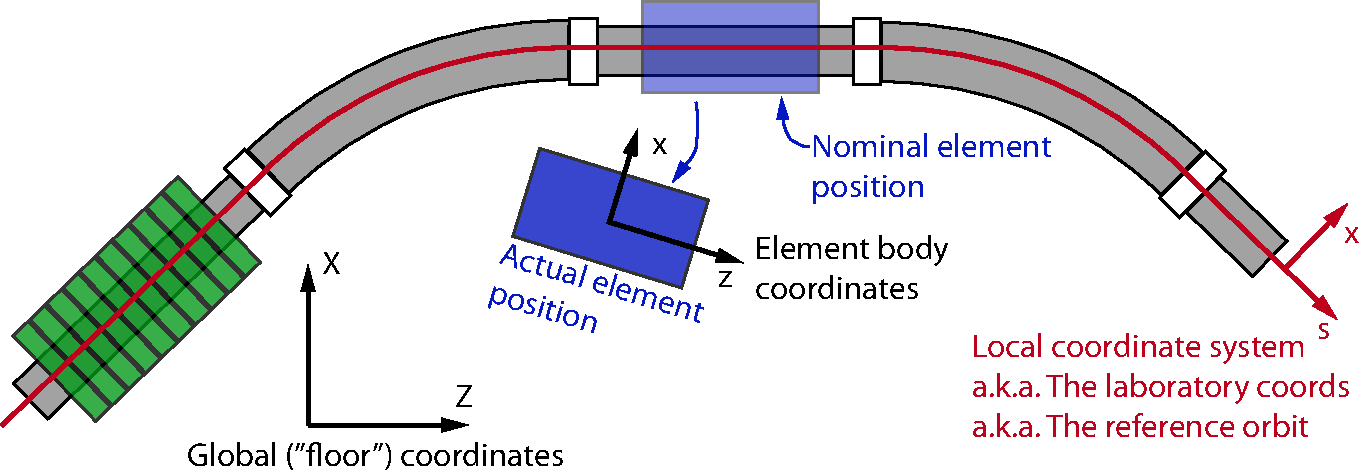
\includegraphics[width=5in]{coordinates.pdf}
  \caption[The three coordinate system used by \bmad.]
{The three coordinate systems used by \bmad:
The \vn{global} (or ``\vn{floor}'') coordinate system is independent of the accelerator.
The \vn{local} curvilinear coordinate system follows the bends of the accelerator. 
Each lattice element has \vn{element body} coordinates which, if the element is not ``misaligned''
is the same as the \vn{local} coordinates.}
  \label{f:coords}
\end{figure}


%-----------------------------------------------------------------------------
\section{Local Reference Coordinates}
\label{s:local.coords}

%-----------------------------------------------------------------------------
\subsection{Local Reference Orbit}
\label{s:ref}
\index{reference orbit|hyperbf}
\index{laboratory coordinates|hyperbf}

\begin{figure}[tb]
  \centering
  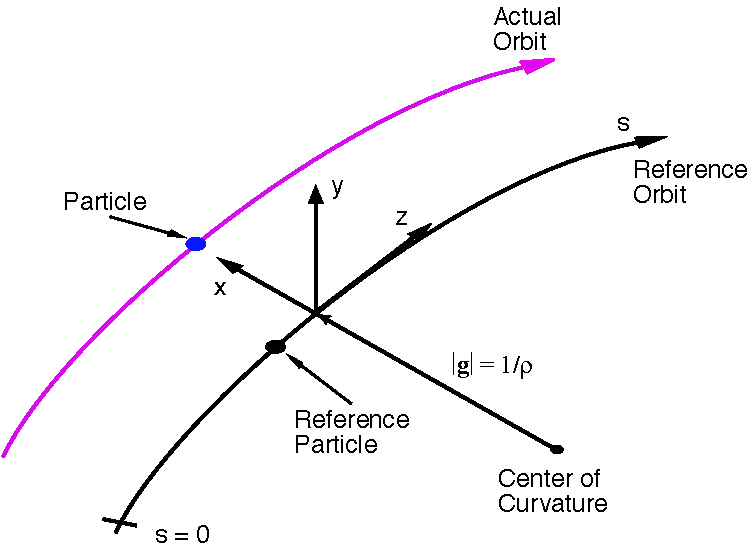
\includegraphics[height=8.4cm]{local-coords.pdf}
  \caption[The local Reference System.]
{The local reference coordinate system. By construction, a particle's
$z$ coordinate is zero.  This is not to be confused with the phase
space $z$ coordinate (\sref{s:phase.space}). The curvature vector
$\bfg$ lies in the $x$-$y$ plane and has a magnitude of $1/\rho$ where
$\rho$ is the bending radius. The $z$-axis will normally be parallel
to the $s$-axis but for \vn{reversed} elements it will be antiparallel.
}
  \label{f:local.coords}
\end{figure}

The \vn{local reference orbit} is the curved path used to define a
coordinate system for describing a particle's position as shown in
\fig{f:local.coords}. The reference orbit is also used for orientating
lattice elements in space. At a given time $t$, a particle's position
can be described by a point on the reference orbit a distance $s$
relative to the reference orbit's zero position plus a transverse
offset. This point on the reference orbit is used as the origin of the
local $(x, y, z)$ coordinate system with the $z$--axis tangent to the
reference orbit. The $z$--axis will generally be pointing in the
direction of increasing $s$ but, as discussed in detail below, will
point counter to $s$ for elements that are \vn{reversed}. The $x$ and
$y$--axes are perpendicular to the reference orbit. As will be shown
later, If the lattice has no vertical bends, the $y$--axis is in the
vertical direction and the $x$--axis is in the horizontal
plane. Notice that, by construction, the particle is always at $z =
0$. The coordinate system so constructed is called the \vn{``local
coordinate system''} or sometimes the \vn{``laboratory coordinate
system''} when there is need to distinguish it from the \vn{``element
coordinate system''} (\sref{s:ele.coords}) which is attached to
the physical element.

There is a separate reference orbit for each branch
(\sref{s:branch.def}) of a lattice. When there are multiple branches,
the reference orbit of a branch must not depend upon the configuration
of branches later on in the array of branches in the lattice. As a
consequence, the reference orbits of the branches can be calculated
one at a time starting with the first branch.

\index{x_offset}\index{y_offset}
\index{x_pitch}\index{y_pitch}\index{wiggler}
Notice that, in a \vn{wiggler}, the reference orbit, which is a
straight line, does {\em not} correspond to the orbit that any actual
particle could travel. Typically the physical element is
centered with respect to the reference curve. However, by specifying offsets, 
pitches or a tilt (See \sref{s:offset}), the physical element may be
arbitrarily shifted with respect to its reference curve. Shifting a
physical magnet with respect to its reference curve generally means
that the reference curve does {\em not} correspond to the orbit that
any actual particle could travel.

Do not confuse this reference orbit (which defines the local
coordinate system) with the reference orbit about which the transfer
maps are calculated (\sref{s:twiss}). The former is fixed by the
lattice while the latter can be any arbitrary orbit.

%-----------------------------------------------------------------------------
\subsection{Reference Orbit Construction: Upstream, Downstream, Entrance, and Exit Element Ends}
\label{s:ref.construct}
\index{reference orbit!construction}
\index{upstream element end}\index{downstream element end}
\index{entrance element end}\index{exit element end}

%--------------------------------------

  \begin{figure}[tb]
  \centering
  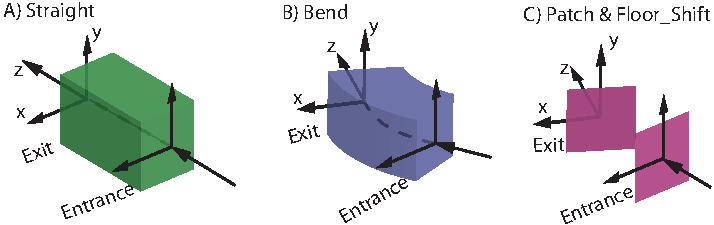
\includegraphics{element-coord-frame.pdf}
\caption[Element LEGO blocks.]{Element reference frame LEGO
blocks. Shown are the blocks along with the entrance and exit
reference frames. The physical element may be displaced in the local
coordinate frame using offsets, tilt, and pitches. A) For straight
line elements the two frames are colinear. B) For bends elements, the
two frames are rotated with respect to each other. C) For \vn{patch}
and \vn{floor_shift} elements the exit frame may be arbitrarily
positioned with respect to the entrance.}
  \label{f:ele.coord.frame}
  \end{figure}

%--------------------------------------

\begin{figure}[tb]
  \centering
  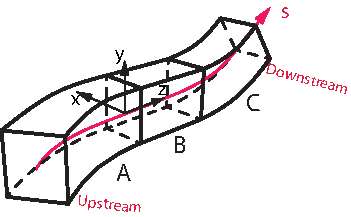
\includegraphics{element-stream.pdf}
  \caption[Element LEGO block concatenation.]{
Element LEGO block concatenation. A) The reference orbit is
constructed by concatenating the LEGO blocks together. B) For normal
(non-reversed) elements the $z$-axis is parallel with the $s$-axis. C)
For \vn{reversed} elements the $z$-axis is antiparallel with the
$s$-axis. By definition, the ``entrance'' and ``exit'' ends of an
element are fixed relative to the element (relative to the $z$-axis)
while the ``upstream'' and ``downstream'' ends are fixed relative to
the $s$-axis.}
  \label{f:stream}
\end{figure}

%--------------------------------------

\index{sbend}\index{rbend}
\index{crystal}\index{mirror}\index{entrance_end}
\index{exit_end}\index{patch}\index{floor_shift}
Another way of thinking about the reference orbit is to imagine that
each element has assigned to it a local coordinate reference frame
assigned to it in the shape of a LEGO block\footnote{Thanks to Dan
Abell for this analogy.} as shown in \fig{f:ele.coord.frame}.  Every
block has an ``\vn{entrance}'' and an ``\vn{exit}'' reference frame.
For most types of elements, the LEGO block for the element is
``straight'' as shown in \fig{f:ele.coord.frame}A. That is, the
reference curve through the block is a straight line segment and the
length of the block is the length of the element. For a \vn{bend}
(\sref{s:bend}), the reference curve through the block is a segment of
a circular arc as shown in \fig{f:ele.coord.frame}B. With a zero
\vn{ref_tilt}, the rotation axis between the entrance and exit frames of a
bend is the $y$-axis (\sref{s:global}). For \vn{patch}
(\sref{s:patch}), and \vn{floor_shift} (\sref{s:floor.ele}) elements,
the exit face can can arbitrarily oriented with respect to the
entrance end. In this case, the reference orbit between the entrance
and exit faces is not defined.

\index{root branch}
Assuming for the moment that there are no \vn{fiducial} elements
present, the construction of the reference orbit starts at the
beginning element of a branch. If the branch is a \vn{root} branch
(\sref{s:lattice.def}), The orientation of the beginning element can
be set via the appropriate positioning statements
(\sref{s:beginning}). If the branch is not a \vn{root} branch, the
position of the beginning element is determined by the position of the
\vn{fork} or \vn{photon_fork} element from which the branch forks
from.

Once the beginning element in a branch is positioned, succeeding
element LEGO blocks are concatenated together as illustrated in
\fig{f:stream}A. When a block is joined, the end of the block that is
mated to the previous block is called the ``\vn{upstream}'' end and
the other end which will be mated to the following block is called the
``\vn{downstream}'' end.  Normally, the \vn{entrance} end of a block
is used as the \vn{upstream} end the \vn{exit} end is used as the
\vn{downstream} end as shown in \fig{f:stream}B. However, for
\vn{reversed} elements (\sref{s:ele.reverse}), the \vn{upstream} end
is the \vn{exit} end of the block and vice versa. To put it another
way, the \vn{entrance} and \vn{exit} end of the blocks reference the
physical element. Thus, for example, the \vn{e1} edge of a bend
(\sref{s:bend}) is always at the \vn{entrance} face and the \vn{e2} is
always at the \vn{exit}face. Also the field of a wiggler is
(\sref{s:wiggler}) is referenced to $z = 0$ which is at the
\vn{entrance} end. The \vn{upstream} and \vn{downstream} ends, on the
other hand, are referenced to the reference orbit and the
\vn{downstream} end always is at a larger $s$ position relative to the
\vn{upstream} end.

In all cases, when a LEGO block is joined to the previous block, the
coordinate system at the mating end of the block (the \vn{upstream}
end) will be aligned with the mating end of the previous block (the
\vn{downstream} end). The situation where one of the blocks is
reversed and the other one not, and neither is a \vn{patch} nor
\vn{floor_shift} element, does not make physical sense since a
particle which is moving downstream, when it comes to the face joining
the blocks will have to magically reverse direction in order to travel
through the next block. Thus, to have normal and reversed elements in
a branch, \vn{reflection} \vn{patches} must be used in between.
Whether it makes physical sense to put a \vn{patch} element next to
another element is more complicated. This depends upon whether the
other element is reversed or not and whether the \vn{patch} is
reversed, whether the \vn{patch} is \vn{reflecting}, and the sign of
\vn{z_offset} for the \vn{patch}. The basic criterion is that a
particle leaving one block must enter the next. See
Section~\sref{s:ex.patch} for an example.

If there are \vn{fiducial} elements, the local reference frame is
constructed beginning at these elements.

%-----------------------------------------------------------------------------

\begin{figure}[tb]
  \centering
  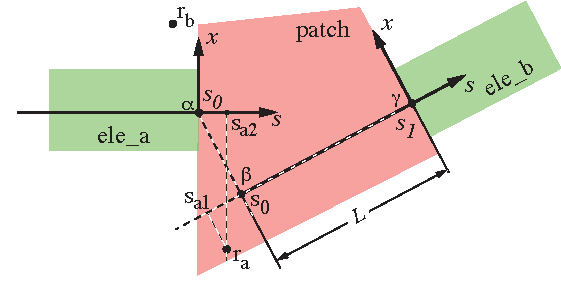
\includegraphics[width=5in]{patch-problem.pdf}
  \caption[The local reference coordinates in a \vn{patch} element.]
{The local reference coordinates in a \vn{patch} element. The
\vn{patch} element, shown schematically as an irregular quadrilateral,
is sandwiched between elements \vn{ele_a} and \vn{ele_b}. \vn{L} is
the length of the \vn{patch}. In this example, the \vn{patch} has a
finite \vn{x_pitch}.}
  \label{f:patch.prob}
\end{figure}

%-----------------------------------------------------------------------------
%-----------------------------------------------------------------------------
\subsection{Patch Element Local Coordinates}
\label{s:patch.prob}
\index{patch}

Generally, if a particle is reasonably near the reference orbit, there
is a one-to-one mapping between the particle's position and $(x, y,
s)$ coordinates. A \vn{patch} (\sref{s:patch}) elements with a
non-zero \vn{x_pitch} or non-zero \vn{y_pitch} breaks the one-to-one
mapping. This is illustrated in \fig{f:patch.prob}.  The \vn{patch}
element, shown schematically as an, irregular quadrilateral, is
sandwiched between elements \vn{ele_a} and \vn{ele_b}. The local
coordinate system with origin at $\alpha$ are the coordinates at the
end of \vn{ele_a}. The coordinates at the end of the \vn{patch} has
its origin labeled $\gamma$. By convention, the length of the patch
\vn{L} is taken to be the longitudinal distance from $\alpha$ to
$\gamma$ with the \vn{patch}'s exit coordinates defining the
longitudinal direction. The ``beginning'' point of the \vn{patch} on
the reference orbit a distance \vn{L} from point $\gamma$ is labeled
$\beta$ in the figure.

In the local $(x, y, s)$ coordinate system a particle at $\alpha$ will
have some value $s = s_0$. A particle at point $\beta$ will have the
same value $s = s_0$ and a particle at $\gamma$ will have $s = s_1 =
s_0 + L$. A particle at point $r_a$ in \fig{f:patch.prob} illustrates
the problem of assigning $(x, y, s)$ coordinates to a given
position. If the particle is considered to be within the region of
\vn{ele_a}, the particle's $s$ position will be $s_{a2}$ which is
greater than the value $s_0$ at the exit end of the element. This
contradicts the expectation that particles within \vn{ele_a} will have
$s \le s_0$.  If, on the other hand, the particle is considered to be
within the \vn{patch} region, the particle's $s$ position will be
$s_{a1}$ which is less than the value $s_0$ at the entrance to the
patch. This contradicts the expectation that a particles within the
\vn{patch} will have $s \ge s_0$.

To resolve this problem, \bmad considers a particle at position $r_a$
to be within the \vn{patch} region. This means that there is, in
theory, no lower limit to the $s$-position that a particle in the
\vn{patch} region can have. This also implies that there is a
discontinuity in the $s$-position of a particle crossing the exit face
of \vn{ele1}. Typically, when particles are translated from the exit
face of one element to the exit face of the next, this \vn{patch}
problem does not appear. It only appears when the track between faces
is considered.

Notice that a particle at position $r_b$ in \fig{f:patch.prob} can
simultaneously be considered to be in either \vn{ele_a} or the
\vn{patch}. While this creates an ambiguity it does not complicate
tracking.

%-----------------------------------------------------------------------------
\section{Global Coordinates}
\label{s:global}
\index{global coordinates|hyperbf}

The Cartesian \vn{global} coordinate system, also called the `floor''
coordinate system, is the coordinate system ``attached to the earth''
that is used to describe the local coordinate system. Following the
\mad\ convention, the \vn{global} coordinate axis are labeled $(X, Y,
Z)$. Conventionally, $Y$ is the ``vertical'' coordinate and $(X, Z)$
are the ``horizontal'' coordinates. To describe how the local
coordinate system is oriented within the global coordinate system,
each point on the $s$-axis of the local coordinate system is
characterized by its $(X, Y, Z)$ position and by three angles $\theta$,
$\phi$, and $\psi$ that describe the orientation of the local coordinate axes
as shown in \fig{f:global.coords}. These three angles are defined as
follows:
\begin{description}
\item[$\theta$ Azimuth angle:] Angle in the $(X, Z)$ plane 
between the $Z$--axis and the projection of the $z$--axis onto the
$(X, Z)$ plane. A positive angle of $\theta = \pi/2$ corresponds to the
projected $z$--axis pointing in the positive $X$ direction.
\item[$\phi$ Pitch (elevation) angle:] Angle between the $z$--axis 
and the $(X,Z)$ plane. A positive angle of $\phi = \pi/2$ corresponds to
the $z$--axis pointing in the positive $Y$ direction.
\item[$\psi$ Roll angle:] Angle of the $x$--axis with respect 
to the line formed by the
intersection of the $(X, Z)$ plane with the $(x, y)$ plane. A
positive $\psi$ forms a right--handed screw with the $z$--axis.
\end{description}

\begin{figure}[tb]
\centering
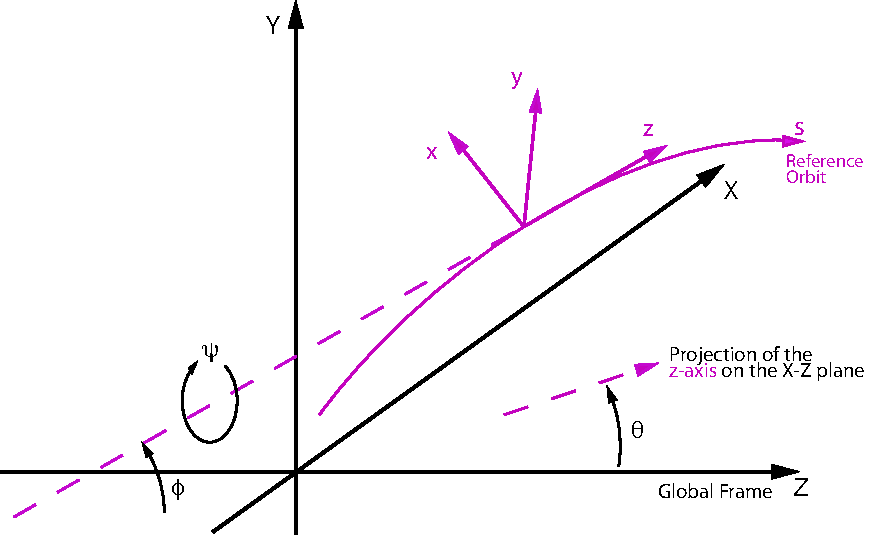
\includegraphics{global-coords.pdf}
\caption[The Global Coordinate System]{The Global Coordinate System.}
\label{f:global.coords}
\end{figure}

\index{beginning statement}
\index{reference orbit!origin in global coordinates}
\index{global coordinates!reference orbit origin}
By default, at $s = 0$, the reference orbit's origin coincides with
the $(X, Y, Z)$ origin and the $x$, $y$, and $z$ axes correspond to
the $X$, $Y$, and $Z$ axes respectively. $\theta$ decreases as one
follows the reference orbit when going through a horizontal bend with
a positive bending angle. This corresponds to $x$ pointing radially
outward. Without any vertical bends, the $Y$ and $y$ axes will
coincide, and $\phi$ and $\psi$ will both be zero. The \vn{beginning}
statement (\sref{s:beginning}) in a lattice file can be use to
override these defaults.

\index{MAD}
Following \mad, the global position of an element is characterized by
a vector $\bfV$ 
\Begineq
  \bfV = 
  \begin{pmatrix}
    X \\ Y \\ Z 
  \end{pmatrix}
\Endeq
The orientation of an element is described by a unitary rotation matrix $\bfW$. The column
vectors of $\bfW$ are the unit vectors spanning the local coordinate axes in the order
$(x, y, z)$. $\bfW$ can be expressed in terms of the orientation angles $\theta$, $\phi$,
and $\psi$ via the formula
\Begineq
  \bfW = \bfR_{y}(\theta) \; \bfR_{-x}(\phi) \; \bfR_{z}(\psi)
  \label{wwww}
\Endeq
where
\Begineq
  \bfR_{y}(\theta) = 
  \begin{pmatrix}
    \cos\theta  & 0 & \sin\theta \\
    0           & 1 & 0          \\
    -\sin\theta & 0 & \cos\theta 
  \end{pmatrix}, \quad
  \bfR_{-x}(\phi) = 
  \begin{pmatrix}
    1 & 0 & 0                \\
    0 & \cos\phi  & \sin\phi \\
    0 & -\sin\phi & \cos\phi 
  \end{pmatrix}, \quad
  \bfR_{z}(\psi) = 
  \begin{pmatrix}
    \cos\psi & -\sin\psi & 0 \\
    \sin\psi &  \cos\psi & 0 \\
    0        &  0        & 1                
  \end{pmatrix}
  \label{wtt0t}
\Endeq
Notice that $\bfR_{-x}(\phi)$, for positive $\phi$, represents a
rotation around the negative $x$-axis.

An alternative representation of the $\bfW$ matrix (or any other rotation matrix) is to
specify the axis $\Bf u$ (normalized to 1) and angle of rotation $\beta$
\Begineq
  \bfW = \begin{pmatrix}
    \cos \beta + u_x^2 \left(1 - \cos \beta \right) & 
    u_x \, u_y \left(1 - \cos \beta \right) - u_z \sin \beta & 
    u_x \, u_z \left(1 - \cos \beta \right) + u_y \sin \beta \\ 
    u_y \, u_x \left(1 - \cos \beta \right) + u_z \sin \beta & 
    \cos \beta + u_y^2\left(1 - \cos \beta \right) & 
    u_y \, u_z \left(1 - \cos \beta \right) - u_x \sin \beta \\ 
    u_z \, u_x \left(1 - \cos \beta \right) - u_y \sin \beta & 
    u_z \, u_y \left(1 - \cos \beta \right) + u_x \sin \beta & 
    \cos \beta + u_z^2\left(1 - \cos \beta \right)
  \end{pmatrix}
  \label{wctux2}
\Endeq

%-----------------------------------------------------------------------------
\subsection{Lattice Element Positioning}
\label{s:ele.pos}

\index{MAD}
\bmad, again following \mad, computes $\bfV$ and $\bfW$ by starting
at the first element of the lattice and iteratively using the
equations
\begin{align}
  \bfV_i &= \bfW_{i-1} \; \bfL_i + \bfV_{i-1}, 
    \label{vwlv} \\
  \bfW_i &= \bfW_{i-1} \; \bfS_i
    \label{wws}
\end{align}
$\bfL_i$ is the displacement vector for the $i$\Th element and matrix
$\bfS_i$ is the rotation of the local reference system of the exit
end with respect to the entrance end. For clarity, the subscript $i$ in 
the equations below will be dripped. For all elements whose
reference orbit through them is a straight line, the corresponding
$\bfL$ and $\bfS$ are
\Begineq
  \bfL = 
  \begin{pmatrix}
      0 \\ 0 \\ L
  \end{pmatrix},
  \quad
  \bfS = 
  \begin{pmatrix}
      1 & 0 & 0 \\ 
      0 & 1 & 0 \\
      0 & 0 & 1
  \end{pmatrix},
  \label{l00l}
\Endeq
Where $L$ is the length of the element. 

%-----------------------------------------------------------------------

\begin{figure}
\centering 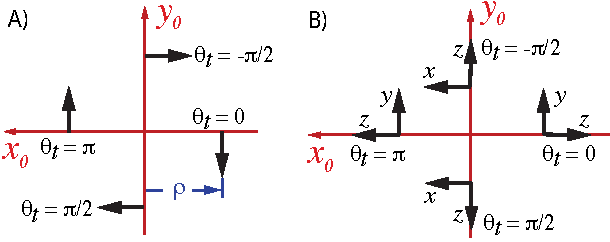
\includegraphics{tilt-bend.pdf} 
\caption[Orientation of a Bend.] 
  {
A) Rotation axes (bold arrows) for four different \vn{ref_tilt} angles
of $\theta_t$ = 0, $\pm \pi/2$, and $\pi$. $(x_0, y_0, z_0)$ are the
local coordinates at the entrance end of the bend with the $z_0$ axis
being directed into the page. Any rotation axis will be displaced by a
distance of the bend radius \vn{rho} from the origin. B) The $(x, y,
z)$ coordinates at the exit end of the bend for the same four
\vn{ref_tilt} angles. In this case the bend angle is taken to be
$\pi/2$.
  }
  \label{f:tilt.bend}
\end{figure}

%-----------------------------------------------------------------------

\index{rbend}\index{sbend}
\index{rho}\index{tilt}\index{angle}
For a \vn{bend}, the axis of rotation is dependent upon the bend's \vn{ref_tilt} angle
(\sref{s:offset}) as shown in \fig{f:tilt.bend}A. The axis of rotation points in the
negative $y_0$ direction for \vn{ref_tilt} = 0 and is offset by the bend radius
\vn{rho}. Here $(x_0, y_0, z_0)$ are the local coordinates at the entrance end of the bend
with the $z_0$ axis being directed into the page in the figure.  For a non-zero
\vn{ref_tilt}, the rotation axis is itself rotated about the $z_0$ axis by the value of
\vn{ref_tilt}. \fig{f:tilt.bend}B shows the exit coordinates for four different values of
\vn{ref_tilt} and for a bend angle \vn{angle} of $\pi/2$.
Notice that for a bend in the horizontal $X-Z$ plane, a positive
bend \vn{angle} will result in a decreasing azimuth angle $\theta$.

For a bend, $\bfS$ is given using \Eq{wctux2} with 
\begin{align}
  \Bf u &= (-\sin\theta_t, -\cos\theta_t, 0) \CRNO
  \beta &= \alpha_b
  \label{ustt}
\end{align}
where $\theta_t$ is the \vn{ref_tilt} angle. The $\bfL$ vector for a \vn{bend} is given by 
\Begineq
  \bfL = \bfR_{z}(\theta_t) \; \bftilde L, \quad
  \bftilde L = 
  \begin{pmatrix}
    \rho (\cos\alpha_b - 1) \\ 0 \\ \rho \, \sin\alpha_b
  \end{pmatrix}
  \label{lrztt}
\Endeq
where $\alpha_b$ is the bend \vn{angle} (\sref{s:bend}) and $\rho$ being the bend radius
(\vn{rho}). Notice that since $\Bf u$ is perpendicular to $z$, the curvilinear reference coordinate
system has no ``torsion''. That is, it is a Frenet-Serret coordinate system.

Note: An alternative equation for \vn{\bfS} for a bend is
 \Begineq
  \bfS = \bfR_{z}(\theta_t) \; \bfR_{y}(-\alpha_b) \; \bfR_{z}(-\theta_t)
  \label{srrr}
\Endeq

The bend transformation above is so constructed that the
transformation is equivalent to rotating the local coordinate system
around an axis that is perpendicular to the plane of the bend. This
rotation axis is invariant under the bend transformation. For example,
for $\theta_t = 0$ (or $\pi$) the $y$-axis is the rotation axis and
the $y$-axis of the local coordinates before the bend will be parallel
to the $y$-axis of the local coordinates after the bend as shown in
\fig{f:tilt.bend}. That is, a lattice with only bends with
$\theta_t = 0$ or $\pi$ will lie in the horizontal plane (this
assuming that the $y$-axis starts out pointing along the $Y$-axis as
it does by default).  For $\theta_t = \pm\pi/2$, the bend axis is the
$x$-axis. A value of $\theta_t = +\pi/2$ represents a downward
pointing bend.

\begin{figure}
  \centering 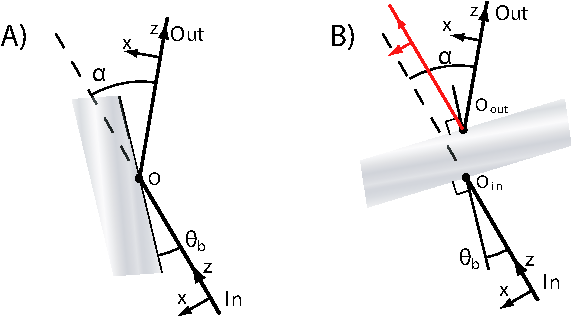
\includegraphics{mirror.pdf} 
\caption[Mirror and crystal geometry] {Mirror and crystal geometry.
The geometry shown here is appropriate for a \vn{ref_tilt} angle of
$\theta_t = 0$.  $\theta_g$ is the bend angle of the incoming
(entrance) ray, and $\alpha_b$ is the total bend
angle of the reference trajectory. A) Geometry for a mirror or a Bragg
crystal. Point $\calO$ is the origin of both the local coordinates
just before and just after the reflection/diffraction. B) Geometry for
a Laue crystal.  Point $\calO_{out}$ is the origin of the coordinates
just after diffraction is displaced from the origin $\calO_{in}$ just
before diffraction due to the finite thickness of the crystal. here
the bend angles are measured with respect to the line that is in
the plane of the entrance and exit coordinates and perpendicular to
the surface. For Laue diffraction, the user has the option of using
the undiffracted beam (shown in red) as the reference trajectory.
  }  
  \label{f:mirror}
\end{figure}

%-----------------------------------------------------------------------------
\subsection{Position Transformation When Transforming Coordinates}
\label{s:pos.trans}

A point $\bfQ_g = (X, Y, Z)$ defined in the global coordinate system,
when expressed in the coordinate system defined by $(\bfV, \bfW)$ is
\Begineq
  \bfQ_{VW} = \bfW^{-1} \left( \bfQ_g - \bfV \right)
  \label{rwrv}
\Endeq
This is essentially the inverse of \Eq{vwlv}. That is, vectors
propagate inversely to the propagation of the coordinate system.

Using \Eq{rwrv} with \Eqs{vwlv}, and \eq{wws}, the transformation of a
particle's position $\bfq = (x,y,z)$ and momentum $\bfP = (P_x, P_y,
P_z)$ when the coordinate frame is transformed from frame
$(\bfV_{i-1}, \bfW_{i-1})$ to frame $(\bfV_i, \bfW_i)$ is
\begin{align}
  \bfq_i &= \bfS_i^{-1} \, \left( \bfq_{i-1} - \bfL_i \right), 
    \label{rwlr} \\
  \bfP_i &= \bfS_i^{-1} \, \bfP_{i-1}
    \label{pps}
\end{align}

Notice that since $\bfS$ (and $\bfW$) is the product of orthogonal
rotation matrices, $\bfS$ is itself orthogonal and its inverse is
just the transpose
\Begineq
  \bfS^{-1} = \bfS^T
\Endeq

%-----------------------------------------------------------------------------
\subsection{Crystal and Mirror Element Coordinate Transformation}
\label{s:mirror.coords}

\index{crystal}\index{mirror}\index{ref_tilt}
A \vn{crystal} element (\sref{s:mirror}) diffracts photons and a
\vn{mirror} element (\sref{s:mirror}) reflects them. For a crystal
setup for Bragg diffraction, and for a mirror, the reference orbit is
modeled as a zero length bend with $\bftilde L = (0, 0, 0)$, as shown
in \fig{f:mirror}A. Shown in the figure is the geometry
appropriate for a \vn{ref_tilt} angle of $\theta_t = 0$ (the rotation axis is
here the $y$-axis). Since the mirror or crystal element is modeled to
be of zero length, the origin points (marked $\calO$ in the figure)
of the entrance and exit local coordinates are the same. For Laue
diffraction, the only difference is that $\bftilde L$ is non-zero due
to the finite thickness of the crystal as shown in
\fig{f:mirror}B. This results in a separation between the
entrance coordinate origin $\calO_{in}$ and the exit coordinate
origin $\calO_{out}$.

In all cases, the total bending angle is
\begin{align}
  \alpha_b &= \text{bragg_angle_in} + \text{bragg_angle_out} &\text{! Crystal} \CRNO
  \alpha_b &= 2 \, \text{graze_angle}                        &\text{! Mirror}
  \label{agg}
\end{align}
With a mirror or Bragg diffraction, the bend angles are measured with
respect to the surface plane. With Laue diffraction the bend angles
are measured with respect to the line in the bend plane perpendicular
to the surface.

For Laue diffraction, the user has the option of using the
undiffracted beam (shown in red) as the reference trajectory.

The orientation of the exit coordinates (the local coordinates after
the reflection) are only affected by the element's \vn{ref_tilt} and
bend angle parameters and is independent of all other parameters such
as the radius of curvature of the surface, etc. The local $z$-axis of
the entrance coordinates along with the $z$-axis of the exit
coordinates define a plane which is called the element's \vn{bend
plane}.  For a mirror, the graze angle is a parameter supplied by the
user. For a crystal, the Bragg angles are calculated so that the
reference trajectory is in the middle of the Darwin curve. Calculation
of the Bragg angles for a crystal is given in
Section~\sref{s:crystal.ref}.

%-----------------------------------------------------------------------------
\subsection{Patch and Floor_Shift Elements Entrance to Exit Transformation}
\label{s:patch.coords}

\index{patch!coordinate transformation}\index{floor_shift!coordinate transformation}
For \vn{patch} (\sref{s:patch}) and \vn{floor_shift} (\sref{s:floor.ele}) elements, the
shift in the exit end reference coordinates is
given by \Eqs{vwlv} and \eq{wws} with 
\begin{align}
  \bfL &= 
    \begin{pmatrix} 
      \text{x_offset} \\ \text{y_offset} \\ \text{z_offset} 
    \end{pmatrix}
    \CRNO
  \bfS &= \bfR_{y} (\text{x_pitch}) \; \bfR_{-x} (\text{y_pitch}) \; \bfR_{z} (\text{tilt})
  \label{swww}
\end{align}

The difference here between \vn{patch} and \vn{floor_shift} elements is that, with a
\vn{patch} element, the shift is relative to the exit end of the previous element while,
for a \vn{floor_shift} element, the shift is relative to the reference point on the 
origin element specified by the \vn{origin_ele} parameter of the \vn{floor_shift}.

%-----------------------------------------------------------------------------
\subsection{Fiducial and Girder Elments Origin Shift Transformation}
\label{s:girder.coords}

\index{girder}\index{fiducial}
For \vn{fiducial} and \vn{girder} elements, the alignment of the
reference coordinates with respect to ``\vn{origin}'' coordinates is
analogous to \Eqs{swww}. Explicitly:
\begin{align}
  \bfL &= 
    \begin{pmatrix} 
      \text{dx_origin} \\ \text{dy_origin} \\ \text{dz_origin}
    \end{pmatrix}
    \CRNO
  \bfS &= \bfR_{y} (\text{dtheta_origin}) \; \bfR_{-x} (\text{dphi_origin}) \; \bfR_{z} (\text{dpsi_origin})
\end{align}

%-----------------------------------------------------------------------------
\subsection{Reflection Patch}
\label{s:reflect.patch}
\index{patch!reflection}

A \vn{Patch} (or a series of patches) that reflects the direction of the \vn{z}-axis is
called a \vn{reflection} \vn{patch}. By ``reflected direction'' it is meant that the dot
product $\Bf z_1 \cdot \Bf z_2$ is negative where $\Bf z_1$ is the $z$-axis vector at the
\vn{entrance} face and $\Bf z_2$ is the $z$-axis vector at the \vn{exit} face. This
condition is equivalent to the condition that the associated $\bfS$ matrix (see \Eq{swww})
satisfy:
\Begineq
  S(3,3) < 0
  \label{s330}
\Endeq
Using \Eq{swww} gives, after some simple algebra, this condition is equivalent to
\Begineq
  \cos(\text{x_pitch}) \, \cos(\text{y_pitch}) < 0
\Endeq
When there are a series of patches, The transformations of all the
patches are concatenated together to form an effective $\bfS$ which
can then be used with \Eq{s330}.

%-----------------------------------------------------------------------------
\section{Transformation Between Laboratory and Element Body Coordinates}
\label{s:lab.body.transform}
\index{laboratory coordinates}
\index{element body coordinates|hyperbf}


The \vn{element body} coordinates are the coordinate system attached to an
element. Without any misalignments, where \vn{``misalignments''} are here defined to be
any offset, pitch or tilt (\sref{s:offset}), the \vn{laboratory} coordinates (\sref{s:ref}) and
\vn{element body} coordinates are the same. With misalignments, the transformation between
\vn{laboratory} and \vn{element body} coordinates depends upon whether the local coordinate
system is straight (\sref{s:straight.mis}) or bent (\sref{s:bend.mis}).

%-----------------------------------------------------------------------------
\subsection{Straight Element Misalignment Transformation}
\label{s:straight.mis}

For straight line elements, given a laboratory coordinate frame $\Lambda_s$ with origin a
distance $s$ from the beginning of the element, misalignments will shift the coordinates
to a new reference frame denoted $E_s$. Since misalignments are defined with respect to
the middle of the element, the transformation between $\Lambda_s$ and $E_s$ is a three
step process:
\Begineq
  \Lambda_s \longrightarrow \Lambda_\text{mid} 
  \longrightarrow E_\text{mid} \longrightarrow E_s
  \label{llee}
\Endeq
where $\Lambda_\text{mid}$ and $E_\text{mid}$ are the laboratory and
element reference frames at the center of the element.

The first and last transformations from $\Lambda_s$ to
$\Lambda_\text{mid}$ and from $E_\text{mid}$ to $E_s$ use \Eqs{vwlv},
\eq{wws}, and \eq{l00l} with the replacement $L \rightarrow L/2 - s$
for the first transformation and $L \rightarrow s - L/2$ for the third
transformation. The middle transformation, by definition of the
offset, pitch and tilt parameters is
\begin{align}
  \bfL &= 
    \begin{pmatrix} 
      \text{x_offset} \\ \text{y_offset} \\ \text{z_offset} 
    \end{pmatrix}
    \CRNO
  \bfS &= \bfR_{y} (\text{x_pitch}) \; \bfR_{-x} (\text{y_pitch}) \; \bfR_{z} (\text{tilt})
  \label{swww2}
\end{align}

Notice that with this definition of how elements are misaligned, the position of a
misaligned element depends only on the offsets, and is independent of the pitches and tilt.

%-----------------------------------------------------------------------------
\subsection{Bend Element Misalignment Transformation}
\label{s:bend.mis}

\index{rbend!coordinate transformation}\index{sbend!coordinate transformation}
\index{roll!coordinate transformation}\index{tilt!coordinate transformation}
For \vn{rbend} and \vn{sbend} elements there is no \vn{tilt} attribute.  Rather, there is
the \vn{roll} attribute and a \vn{ref_tilt} attribute. The latter affects both the
reference orbit and the bend position (\sref{s:bend.orient}). Furthermore, \vn{ref_tilt}
is calculated with respect to the coordinates at the beginning of the bend while, like
straight elements, \vn{roll}, offsets, and pitches are calculated with respect to the
center of the bend. The different reference frame used for \vn{ref_tilt} versus everything
else means that five transformations are needed to get from the laboratory frame to the
element body frame (see \Eq{llee}). Symbolically:
\Begineq
  \Lambda_s \longrightarrow \Lambda_\text{mid} 
  \longrightarrow \Omega_\text{mid} \longrightarrow \Omega_0
  \longrightarrow E_0 \longrightarrow E_s
\Endeq

The first transformation, $\Lambda_s$ to $\Lambda_\text{mid}$, from laboratory coordinates
at a distance $s$ from the beginning of the element to coordinates at the center the the
bend is a rotation around the center of curvative of the bend and is given by \Eqs{vwlv}
and \eq{wws} with \Eqs{ustt} and \eq{lrztt} with the substitution $\alpha_b \rightarrow (L/2
- s)/\rho$.

The second transformation $\Lambda_\text{mid}$ to $\Omega_\text{mid}$ at the center of the
element adds in the misalignments (Note that the coordinate frame $\Omega_\text{mid}$ is
neither a laboratory frame or an element frame so hence the use of a different symbol
$\Omega$). Explicitly, the $\Lambda_\text{mid} \longrightarrow \Omega_\text{mid}$ transformation is
\begin{align}
  \bfL &= \bfL_\text{off} + 
    \left[ \bfR_z(\text{roll}) - \Bf1 \right] \; \bfR_z(\theta_t) \; \bfR_{y}(\alpha_b/2) \; \bfL_c \CRNO
  \bfS &= \bfR_{y}(\text{x_pitch}) \; \bfR_{-x}(\text{y_pitch}) \; \bfR_z(\text{roll})
  \label{lcmis}
\end{align}
where
\Begineq
  \bfL_c = 
    \begin{pmatrix}
      \rho (\cos(\alpha_b/2) - 1) \\ 0 \\ \rho \, \sin(\alpha_b/2)
    \end{pmatrix}
  , \qquad
  \bfL_\text{off} = 
    \begin{pmatrix} 
      \text{x_offset} \\ \text{y_offset} \\ \text{z_offset} 
    \end{pmatrix}
\Endeq
The reason why $\bfL$ has a different form from straight line elements
is due to the fact that the axis of rotation for a \vn{roll} is
displaced from the $z$-axis of the coordinate system at the center of
the bend (see \fig{f:roll}).

The third transformation from $\Omega_\text{mid}$ to $\Omega_0$ is
like the first transformation and rotates from the center of the bend
to the beginning. Again \Eqs{ustt} and \eq{lrztt} are used with the 
substitution $\alpha_b \rightarrow -L/2\rho$.

The fourth transformation $\Omega_0$ to $E_0$ tilts the referece frame
by an amount \vn{ref_tilt}:
\Begineq
  \bfL = 0, \quad
  \bfS = \bfR_{z}(\theta_t)
  \label{l0sr}
\Endeq

The fifth and final transformation, $E_0$ to $E_s$, like the first and
third, rotates around the center of the bend but in this case, since
we are dealing with element coordinates, the \vn{ref_tilt} is ignored.
That is, \Eqs{ustt} and \eq{lrztt} are used with the substitutions
$\theta_t \rightarrow 0$ and $\alpha_b \rightarrow L/\rho$.

Notice that with this definition of how elements are misaligned, the position of a
misaligned element depends only on the offsets, and is independent of the pitches and tilt.

%-----------------------------------------------------------------------------
\section{Phase Space Coordinates}
\label{s:phase.coords}
\index{phase space coordinates|hyperbf}

%-----------------------------------------------------------------------------
\subsection{Reference Particle, Reference Energy, and Reference Time}
\label{s:ref.energy}
\index{reference particle|hyperbf}
\index{reference energy|hyperbf}
\index{reference time|hyperbf}

The \vn{reference energy} and \vn{reference time} are needed in
evaluating the phase space coordinates of charged particles
(\sref{s:phase.space}).  

All lattice elements, except for controller elements, have an
associated \vn{reference energy} energy.  The reference energy at the
start of a lattice's \vn{root branch} (\sref{s:branch.def}) is set in
the lattice file by setting the reference momentum (\vn{p0c}) or total
energy (\vn{E_tot}) using a \vn{parameter} (\sref{s:param}) or
\vn{beginning} (\sref{s:beginning}) statement. For other branches, the
energy at the start of the branch is set using the appropriate line
parameter (\sref{s:beginning}) statement.

\index{custom!reference energy}\index{em_field!reference energy}
\index{hybrid!reference energy}\index{lcavity!reference energy}
\index{patch!reference energy}
For most elements, the reference energy is the same as the reference
energy of the preceeding element. The following elements are
exceptions:
\begin{example}
  custom
  em_field
  hybrid
  lcavity
  patch
\end{example}
The reference energy of these elements is determined by tracking a
particle (the ``\vn{reference particle}'') through the element with the
particle starting on the reference orbit and whose energy is equal to
the reference energy.  The energy of the particle at the downstream
end is the reference energy of the element.

\index{wiggler!reference time}
Besides the reference energy, lattice elements have an associated
\vn{reference time} which is computed, for most elements, by the
time-of-flight of the \vn{reference particle} assuming that the
reference particle is following the reference orbit. Exceptions are
\vn{wiggler} elements which uses the time-of-flight of the actual
undulating trajectory. [Actually what is used in the computation of the
$z$ phase space coordinate (\Eq{zbctt}) is the sum of reference time
deltas of the elements that a particle has passed through. It is not
possible to assign a unique reference time to an element when particles
are recirculating through elements as in a storage ring.]

%-----------------------------------------------------------------------------
\subsection{Charged Particle Phase Space Coordinates}
\label{s:phase.space}
\index{phase space coordinates|hyperbf}

\begin{figure}
\centering 
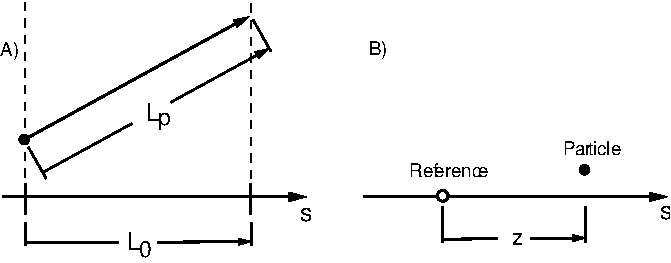
\includegraphics{canonical-z.pdf} 
\caption[Interpreting phase space $z$ at constant velocity.]
{Interpreting phase space $z$ at constant velocity: A) The change in $z$
going through an element of length $L_0$ is $L_0 - L_p$.  B) At
constant time, $z$ is the longitudinal distance between the reference
particle and the particle.}
\label{f:canonical.z}
\end{figure}

For charged particles (more correctly, for everything but photons
(\sref{s:photon.phase.space})), \bmad uses the canonical phase space
coordinates
\Begineq
  \Bf r(s) = (x, p_x, y, p_y, z, p_z)
\Endeq
The longitudinal position $s$ is the independent variable instead of
the time. $x$ and $y$, are the transverse coordinates of the particle
as shown in~\fig{f:local.coords}. Note that $x$ and $y$ are independent
of the position of the reference particle.

The phase space momenta $p_x$ and $p_y$ are normalized by the
reference (sometimes called the design) momentum $P_0$
\begin{align}
  p_x = &\frac{P_x}{P_0} \CRNO
  p_y = &\frac{P_y}{P_0}
  \label{ppp}
\end{align}
where $P_x$ and $P_y$ are respectively the $x$ and $y$ momentums.

\index{lcavity}\index{rfcavity}
The phase space $z$ coordinate is 
\begin{align}
  z(s) &= -\beta(s) \, c \, (t(s) - t_0(s)) \CRNO
    &\equiv - \beta(s) \, c \, \Delta t(s)
  \label{zbctt}
\end{align}
$t(s)$ is the time at which the particle is at position $s$, $t_0(s)$
is the time at which the reference particle is at position $s$, and
$\beta$ is $v/c$ with $v$ being the particle velocity (and not the
reference velocity). The reference particle is, by definition,
``synchronized'' with elements whose fields are oscillating and
therefore the actual fields a particle will see when traveling through
such an element will depend upon the particle's phase space $z$. For
example, the energy change of a particle traveling through an
\vn{lcavity} (\sref{s:lcav}) or \vn{rfcavity} (\sref{s:rfcav}) element
is $z$ dependent. Exception: With absolute time tracking
(\sref{s:rf.time}) fields are tied to the absolute time and not $z$.

If the particle's velocity is constant, and is
the same as the velocity of the reference particle (for example, at
high energy where $\beta = 1$ for all particles), then $\beta \, c \,
t$ is just the path length. In this case, the change in $z$ going
through an element is
\Begineq
  \Delta z = L_0 - L_p
\Endeq
where, as shown in \fig{f:canonical.z}A, $L_0$ is the path
length of the reference particle (which is just the length of the
element) and $L_p$ is the path length of the particle in traversing
the element.  Another way of interpreting phase space $z$ is that, at
constant $\beta$, and constant time, $z$ is the longitudinal distance
between the particle and the reference particle as shown in
\fig{f:canonical.z}B. with positive $z$ indicating that the
particle is ahead of the reference particle.

Do not confuse the phase space $z$ with the $z$ that is the particle's
longitudinal coordinate in the local reference frame as shown in
\fig{f:local.coords}. By construction, this latter $z$ is
always zero.

Notice that if a particle gets an instantaneous longitudinal kick so
that $\beta$ is discontinuous then, from \Eq{zbctt}, phase space $z$ is
discontinuous even though the particle itself does not move in
space. In general, from \Eq{zbctt}, The value of $z$ for a particle at
$s_2$ is related to the value of $z$ for the particle at $s_1$ by
\Begineq
  z_2 = \frac{\beta_2}{\beta_1} \, z_1 - 
  \beta_2 \, c \, (\Delta t_2 - \Delta t_1)
  \label{zbbzb}
\Endeq
$\Delta t_2 - \Delta t_1$ can be interpreted as the difference in
transit time, between the particle and the reference particle, in going
from $s_1$ to $s_2$.

The longitudinal phase space momentum $p_z$ is given by
\begin{equation}
  p_z = \frac{\Delta P}{P_0} \equiv \frac{P - P_0}{P_0}
  \label{ppppp}
\end{equation}
where $P$ is the momentum of the particle. For ultra--relativistic particles
$p_z$ can be approximated by
\begin{equation}
  p_z = \frac{\Delta E}{E_0}
\end{equation}
\index{lcavity}
where $E_0$ is the reference energy (energy here always refers to the
total energy) and $\Delta E = E - E_0$ is the deviation of the
particle's energy from the reference energy. For an \vn{Lcavity}
element (\sref{s:lcav}) the reference momentum is {\it not} constant
so the tracking for an \vn{Lcavity} is not canonical.

\index{phase space coordinates!MAD convention}
\index{MAD!phase space convention}
\mad uses a different coordinate system where $(z, p_z)$ is
replaced by $(-c\Delta t, p_t)$ where $p_t \equiv \Delta E / P_0
c$. For highly relativistic particles the two coordinate systems are
identical.

\index{paraxial approximation}
\index{bmad_standard!tracking method}
\vn{Bmad_standard} (\sref{c:methods}) tracking and transfer matrix
calculations use the small angle (paraxial) approximation where it is
assumed that $p_x, p_y \ll 1$. With this approximation, the
relationship, between the phase space momenta and the slopes $x' \equiv
dx/ds$ and $y' \equiv dy/ds$ is
\begin{align}
  x' &\approx \frac{p_x}{1 + p_z} (1 + g x) \\
  y' &\approx \frac{p_y}{1 + p_z} (1 + g x) 
  \label{xpa1p}
\end{align}
$g = 1/\rho$ is the curvature function with $\rho$ being the radius of
curvature of the reference orbit and it has been assumed that the
bending is in the $x$--$z$ plane. 

With the paraxial approximation, and in the relativistic limit, the
change in $z$ with position is
\Begineq
  \frac{dz}{ds} = -g \, x - \frac{1}{2} (x'^2 + y'^2)
\Endeq
This shows that in a linac, without any bends, the $z$ of a particle
always decreases.

A particle can also have a spin. The spin is characterized by the
spinor $\Psi = \left( \psi_{1}, \psi_{2} \right)^{T}$ where
$\psi_{1,2}$ are complex numbers (\sref{s:spin.dyn}).

\index{phase space coordinates!PTC convention}
\index{FPP/PTC!phase space convention}
For those programmers using the PTC\index{PTC/FPP} software package
directly (ignore this if you don't know what is being talked about
here), \'Etienne Forest uses, by default, a different phase space
coordinates which uses $(t, \Delta E/P_0)$ instead of \bmad's $(z,
\Delta P/P_0)$. See Chapter~\sref{c:ptc} for more details. Which phase
space coordinates are ``better'' is a matter of taste. In general, the
equations of motion in a magnetic field are simpler with $(z, \Delta
P/P_0)$ while the equations of motion in an electric field are simple
with $(t, \Delta E/P_0)$.

%-----------------------------------------------------------------------------
\subsection{Time-based Phase Space Coordinates}
\label{s:time.phase.space}
\index{time!phase space coordinates|hyperbf}

Some specialized routines (for example, time Runge Kutta tracking) use
the time $t$ as the independent variable for charged particle
tracking. This is useful when particles can reverse direction since the normal
$z$ based tracking cannot handle this. Direction reversal can happen, for example,
with low energy ``dark current'' electrons that are generated at the
walls of the vacuum chamber.

When the tracking is time based the phase space coordinates are:
\Begineq
  (x, c \, p_x, y, c \, p_y, z, c \, p_s)
\Endeq
The positions $x$, $y$, and $z$ are the same as with phase spac
coordinates (\sref{s:phase.space}). The momenta are defined as
\begin{align}
c p_x &\equiv m c^2 \gamma \beta_x \CRNO
c p_y &\equiv m c^2 \gamma \beta_y \\
c p_s &\equiv m c^2 \gamma \beta_s, \nonumber
\end{align}
and internally are stored in units of eV.

%-----------------------------------------------------------------------------
\subsection{Photon Phase Space Coordinates}
\label{s:photon.phase.space}
\index{photon!phase space coordinates|hyperbf}

The phase space coordinates discussed above implicitly assume that
particles are traveling longitudinally in only one direction. That is,
the sign of the $s$ component of the momentum cannot be determined
from the phase space coordinates. This is generally fine for tracking
high energy beams of charged particles but for photon tracking this
would oftentimes be problematical. For photons, therefore, a different
phase space is used:
\Begineq
  (x, \beta_x, y, \beta_y, z, \beta_z)
  \label{xbybzb}
\Endeq
Here $(\beta_x, \beta_y, \beta_z)$ is the normalized photon velocity with
\Begineq
  \beta_x^2 + \beta_y^2 + \beta_z^2 = 1 
  \label{bbb1}
\Endeq
and $(x, y, z)$ are the reference orbit coordinates with $z$ being the
distance from the start of the lattice element the photon is in.

In \bmad, the information associated with a photon include its phase
space coordinates and time along with the photon energy and four
parameters $E_x, \phi_x$, and $E_y, \phi_y$ specifying the intensity
and phase of the field along the $x$ and $y$ axes transverse to the
direction of propagation.  the field in the vicinity of the photon is
\begin{align}
  E_x (\Bf r, t) &\sim E_x \, e^{i (k \, (z - z_0) - \omega \, (t - t_{ref}) + \phi_x)} \CRNO
  E_y (\Bf r, t) &\sim E_y \, e^{i (k \, (z - z_0) - \omega \, (t - t_{ref}) + \phi_y)} 
  \label{ertee}
\end{align}
where $z_0$ is the photon $z$ position and and $t_ref$ is the reference time.

The normalization between field and intensity is dependent upon the
particular parameters of any given simulation and so must be
determined by the program using \bmad.


\chapter{Electromagnetic Fields}

%-----------------------------------------------------------------
\section{Magnetic Static Multipole Fields}
\label{s:mag.field}
\index{magnetic fields|hyperbf}

\index{MAD}
Start with the assumption that the local magnetic field has no longitudinal component
(obviously this assumption does not work with, say, a solenoid).  Following \mad, ignoring
skew fields for the moment, the vertical magnetic field along the $y = 0$ axis is expanded
in a Taylor series
\Begineq
  B_y(x, 0) = \sum_n B_n \, \frac{x^n}{n!}
  \label{byx0b}
\Endeq
Assuming that the reference orbit is locally straight (there are correction terms if the
Reference Orbit is curved), the field is
\begin{alignat}{5}
  B_x &=           &&B_1 y \plus         &&B_2 \, xy       
                   && \plus && \frac{1}{6} B_3 (3x^2 y - y^3) \plus \ldots \\
  B_y &= B_0 \plus &&B_1 x + \frac{1}{2} &&B_2 (x^2 - y^2) 
                   && \plus && \frac{1}{6} B_3 (x^3 - 3x y^2) \plus \ldots
\end{alignat}
For some fields, the normalized integrated multipole $K_nL$ can be used when specifying
magnetic multipole components
\index{multipole!KnL, Tn|hyperbf}
\Begineq
  K_nL \equiv \frac{q \, L \, B_n}{P_0}
\Endeq
where $q$ is the charge of the reference particle (in units of the elementary charge), $L$
is the element length, and $P_0$ is the reference momentum (in units of eV/c).  Note that
$P_0/q$ is sometimes written as $B\rho$. This is just an old notation where $\rho$ is the
bending radius of a particle with the reference energy in a field of strength $B$.

The kicks $\Delta p_x$ and $\Delta p_y$ that a
particle experiences going through a multipole field is
\begin{alignat}{5}
  \Delta p_x & = \frac{-q \, L \, B_y}{P_0} \label{pqlbp1} \\
             & = -K_0 L \;-\; 
             && K_1 L \, x \plus 
             \frac{1}{2} && K_2 L (y^2 - x^2) && \plus 
             && \frac{1}{6} K_3 L (3x y^2 - x^3) \plus \ldots 
             \nonumber \\
  \Delta p_y & = \frac{q \, L \, B_x}{P_0} \label{pqlbp2} \\
             & =     
             && K_1 L \, y \plus 
             && K_2 L \, xy && \plus 
             && \frac{1}{6} K_3L (3x^2 y - y^3) \plus \ldots \nonumber 
\end{alignat}
A positive $K_1L$ quadrupole component gives
horizontal focusing and vertical defocusing. The general form is
\begin{align}
  \Delta p_x &= \sum_{n = 0}^{\infty} \frac{K_n L}{n!} 
             \sum_{m = 0}^{\lfloor \frac{n}{2} \rfloor}
             \begin{pmatrix} n \cr 2m \end{pmatrix} \,
             (-1)^{m+1} \, x^{n-2m} \, y^{2m} \\
  \Delta p_y &= \sum_{n = 0}^{\infty} \frac{K_n L}{n!} 
             \sum_{m = 0}^{\lfloor \frac{n-1}{2} \rfloor}
             \begin{pmatrix} n \cr 2m+1 \end{pmatrix} \,
             (-1)^{m} \, x^{n-2m-1} \, y^{2m+1}
\end{align}
where $\lfloor\alpha\rfloor$ means round down to the integer equal to or less than $\alpha$ and 
$a \choose b$ (``a choose b'') denotes a binomial coefficient.

\index{multipole!KnL, Tn|hyperbf}
So far only the normal components of the field have been
considered. If the fields associated with a particular $B_n$ multipole
component are rotated in the $(x, y)$ plane by an angle $\theta_n$, the
magnetic field at a point $(x,y)$ can be expressed in complex notation
as
\Begineq
  B_y(x,y) + i B_x(x,y) = 
    \frac{1}{n!} B_n e^{-i(n+1)\theta_n} \, e^{i n \theta} \, r^n 
  \label{bib1nb}
\Endeq
where $(r, \theta)$ are the polar coordinates of the point $(x, y)$.

\index{multipole}
Note that, for compatibility with MAD, the $K0L$ component of a \vn{Multipole} element
rotates the reference orbit essentially acting as a zero length bend. This is not true
for multipoles of any other type of element.

Instead of using magnitude $K_n$ and rotation angle $\theta_n$,
Another representation is using normal $\wt K_n$ and skew $\wt
KS_n$. The conversion between the two are
\begin{align}
  \wt K_n  &= K_n \, \cos((n + 1) \theta_n) \CRNO
  \wt KS_n &= K_n \, \sin((n + 1) \theta_n) 
\end{align}

\index{multipole!an, bn|hyperbf}
Another representation of the magnetic field used by \bmad divides
the fields into normal $b_n$ and skew $a_n$ components. In terms of
these components the magnetic field for the $n$\Th\ order multipole is
\Begineq
  \frac{q \, L}{P_0} \, (B_y + i B_x) = (b_n + i a_n) \, (x + i y)^n
  \label{qlpbb}
\Endeq
The $a_n$, $b_n$ representation of multipole fields can be used in elements such as
quadrupoles, sextupoles, etc. to allow ``error'' fields to be represented.  
The conversion between $(a_n, b_n)$ and $(K_nL, \theta_n)$ is
\Begineq
  b_n + i a_n = \frac{1}{n!} \, K_nL \, e^{-i(n+1)\theta_n}
\Endeq
or
\begin{align}
  K_n L &= n! \, \sqrt{a_n^2 + b_n^2} \\
  \tan[(n+1) \theta_n] &= \frac{-a_n}{b_n}
\end{align}
To convert a normal magnet (a magnet with no skew component) into a skew
magnet (a magnet with no normal component) the magnet should be rotated
about its longitudinal axis with a rotation angle of
\Begineq
  (n+1) \theta_n = \frac{\pi}{2}
\Endeq
For example, a normal quadrupole rotated by $45^\circ$ becomes a
skew quadrupole.

\index{r0_mag}
\index{F (multipole scale factor)}
The actual $a_n$, $b_n$ values used in particle tracking are scaled from the input values given in
the lattice file. There are two scale factors that are applied. The first scale factor is used if
the \vn{field_master} attribute (\sref{s:field.master}) is True (default is False) for an element so
that the multipole values specified in the lattice file are not reference energy normalized
\Begineq
  \bigl[ a_n, b_n \bigr] \longrightarrow
  \bigl[ a_n, b_n \bigr] \cdot \frac{q}{P_0}
  \label{ababq}
\Endeq

The second scaling is applied when the multipoles are associated with a non
\vn{AB_Multipole} element and if the \vn{scale_multipoles} attribute (\sref{s:multip}) is
\vn{True}. This scaling uses a measurement radius $r_0$ and a scale factor $F$:
\Begineq
  \bigl[ a_n, b_n \bigr] \longrightarrow
  \bigl[ a_n, b_n \bigr]
  \cdot F \cdot \frac{r_0^{n_\text{ref}}}{r_0^n}
  \label{ababf}
\Endeq
$r_0$ is set by the \vn{r0_mag} attribute of an element. $F$ and $n_\text{ref}$ are set
automatically depending upon the type of element as shown in Table~\ref{t:ab}. The
$\gamma_p$ term is

\index{kicker}\index{hkicker}\index{vkicker}\index{ac_kicker}
\index{rbend}\index{sbend}\index{elseparator}
\index{quadrupole}\index{solenoid}\index{sol_quad}
\index{sextupole}\index{octupole}
\begin{table}[ht]
\centering
\begin{tabular}{lll} \toprule
\tt
  {\em Element} & $F$                              & $n_\text{ref}$ \\ \midrule
  \vn{Elseparator} & $\sqrt{{\tt Hkick}^2 + {\tt Vkick}^2}$ & 0 \\
  \vn{Hkicker}     & Kick                                   & 0 \\
  \vn{Kicker},\vn{AC_Kicker}
                   & $\sqrt{{\tt Hkick}^2 + {\tt Vkick}^2}$ & 0 \\
  \vn{Rbend}       & G * L                                  & 0 \\
  \vn{Sbend}       & G * L                                  & 0 \\
  \vn{Vkicker}     & Kick                                   & 0 \\
  \vn{Wiggler}     & $\dsfrac{2 \, c \, {\tt L\_pole} \, B_{max}}{\pi \, {\tt p0c}}$ 
                                                            & 0 \\
  \vn{Quadrupole}  & K1 * L                                 & 1 \\
  \vn{Sol_Quad}    & K1 * L                                 & 1 \\
  \vn{Solenoid}    & KS * L                                 & 1 \\
  \vn{Sextupole}   & K2 * L                                 & 2 \\
  \vn{Octupole}    & K3 * L                                 & 3 \\ \bottomrule
\end{tabular}
\caption{$F$ and $n_\text{ref}$ for various elements.}
\label{t:ab}
\end{table}

%-----------------------------------------------------------------
\section{Electric Static Multipole Fields}
\label{s:elec.field}
\index{electric fields}

Except for the \vn{elseparator} element, \bmad specifies DC electric fields using normal
$b_{en}$ and skew $a_{en}$ components (\sref{s:multip}. The potential $\phi_n$ for the
$n$\Th\ order multipole is
\Begineq
  \phi_n = -\re \left[ \frac{b_{en} - i a_{en}}{n + 1} \, \frac{(x + i y)^{n+1}}{r_0^n} \right]
  \label{pbian1}
\Endeq
where $r_0$ is a ``measurement radius'' set by the \vn{r0_elec} attribute of an element
(\sref{s:multip}).

The electric field for the $n$\Th order multipole is
\Begineq
  E_x - i E_y = (b_{en} - i a_{en}) \, \frac{(x + i y)^n}{r_0^n}
  \label{exiey}
\Endeq
Notice that the magnetic multipole components $a_n$ and $b_n$ are normalized by the
element length, reference charge, and reference momentum (\Eq{qlpbb}) while their electric
counterparts are not.

Using the paraxial approximation, The kick given a particle due to the electric field is
\Begineq
  \frac{dp_x}{ds} = \frac{q \, E_x}{\beta \, P_0 \, c}, \qquad \frac{dp_y}{ds} = \frac{q \, E_y}{\beta \, P_0 \, c}
\Endeq
Where $\beta$ is the normalized velocity.

%-----------------------------------------------------------------
\section{Exact Multipole Fields in a Bend}
\label{s:field.exact}

For static magnetic and electric multipole fields in a bend, the spacial dependence of the
field is different from multipole fields in an element with a straight geometry as given
by \Eqs{qlpbb} and \eq{exiey}. The analysis of the multipole fields in a bend here follows
McMillan\cite{b:mcmillan}.  

In the rest of this section, normalized coordinates $\rw = r / \rho$, $\xw / = x /
\rho$, and $\yw = y / \rho$ will be used where $\rho$ is the bending radius of the
reference coordinate system, $r$ is the distance, in the plane of the bend, from the bend
center to the observation point, $x$ is the distance in the plane of the from the reference
coordinates to the observation point and $y$ is the distance out-of-plane. With this
convention $\rw = 1 + \xw$.

An electric or magnetic multipole can be characterized by a scalar potential $\phi$ with
the field given by $-\nabla \phi$.  The potential is a solution to Laplace's equation
\Begineq
  \frac{1}{\rw} \, \frac{\partial}{\partial \, \rw} 
  \left( \rw \, \frac{\partial \, \phi}{\partial \, \rw} \right) +
  \frac{\partial^2 \phi}{\partial \, \yw^2} = 0
\Endeq
As McMillian shows, it is also possible to calculate the magnetic field by constructing the
appropriate vector potential. However, from a practical point of view, it is simpler to use the
scalar potential for both the magnetic and electric fields.

Solutions to Laplace's equation can be found in form
\Begineq
  \phi_{n}^r = \frac{-1}{1+n} \sum_{p = 0}^{\lfloor (n+1)/2 \rfloor} 
             \begin{pmatrix} n + 1 \cr 2 \, p \end{pmatrix} \,
             (-1)^{p} \, F_{n+1-2p}(\rw) \, \yw^{2p}
  \label{pspn1}
\Endeq
and in the form
\Begineq
  \phi_{n}^i = \frac{-1}{1+n} \sum_{p = 0}^{\lfloor n/2 \rfloor} 
             \begin{pmatrix} n + 1 \cr 2p +1 \end{pmatrix} \,
             (-1)^{p} \, F_{n-2p}(\rw) \, \yw^{2p+1}
  \label{pspn2}
\Endeq
where $a \choose b$ (``a choose b'') denotes a binomial coefficient, $n$ is the order
number which can range from 0 to infinity, $\lfloor\alpha\rfloor$ means round down to the
integer equal to or less than $\alpha$. [Notice that here $n$ is related to $m$ in
McMillian's paper by $m = n + 1$. Also note that the $\phi^r$ and $\phi^i$ here have a
normalization factor that is different from McMillian.]

In \Eq{pspn2} the $F_p(\rw)$ are related by
\Begineq
  F_{p+2} = (p + 1) \, (p + 2) \, \int_1^{\rw} \frac{d\rw}{\rw} 
  \left[ \int_1^{\rw} d\rw \, \rw \, F_{p} \right]
\Endeq
with the ``boundary condition'':
\begin{align}
  F_0(\rw) &= 1 \CRNO
  F_1(\rw) &= \ln \, \rw
\end{align}
This condition ensures that the number of terms in the sums in \Eqs{pspn1} and \eq{pspn2}
are finite. With this condition, all the $F_p$ can be constructed:
\begin{align}
  F_1 &= \ln \, \rw = \xw - \frac{1}{2}\xw^2 + \frac{1}{3}\xw^3 - \ldots \CRNO
  F_2 &= \frac{1}{2} (\rw^2 - 1) - \ln \rw = \xw^2 - \frac{1}{3}\xw^3 + \frac{1}{4} \xw^4 - \ldots \CRNO
  F_3 &= \frac{3}{2} [-(\rw^2 - 1) + (\rw^2 + 1) \ln \rw] = \xw^3 - \frac{1}{2} \xw^4 + \frac{7}{20} \xw^5 - \ldots 
         \label{ffff} \\
  F_4 &= 3 [ \frac{1}{8} (\rw^4 - 1) + \frac{1}{2} (\rw^2 - 1) - (\rw^2 + \frac{1}{2}) \ln \rw] = 
         \xw^4 - \frac{2}{5} \xw^5 + \frac{3}{10} \xw^6 - \ldots \CRNO
  &\text{Etc...} \nonumber
\end{align}
In terms of implementing these functions on a computer, the exact $\rw$-dependent functions are
problematical due to round off error near $\xw = 0$. For example, Evaluating $F_4(\rw)$ at $\xw =
10^{-4}$ results in a complete loss of accuracy (no significant digits!) when using double precision
numbers. In practice, \bmad uses a Pade approximant for $\xw$ small enough and then switches to the
$\rw$-dependent formulas for $\xw$ away from zero.

For magnetic fields, the ``real'' $\phi_n^r$ solutions will correspond to skew fields and the
``imaginary'' $\phi_n^i$ solutions will correspond to normal fields
\Begineq
  \bfB = -\frac{P_0}{q \, L} \, 
    \sum_{n = 0}^\infty \rho^n \, \left[ a_n \, \widetilde \nabla \phi_n^r + b_n \, \widetilde \nabla \phi_n^i \right]
  \label{bpql}
\Endeq
where the gradient derivatives of $\widetilde \nabla$ are with respect to the normalized
coordinates. In the limit of infinite bending radius $\rho$, the above equations converge
to the straight line solution given in \Eq{qlpbb}.

For electric fields, the ``real'' solutions will correspond to normal fields and the
``imaginary'' solutions are used for skew fields
\Begineq
  \bfE = -\sum_{n = 0}^\infty \rho^n \, \left[ a_{en} \, \widetilde \nabla \phi_n^i + 
  b_{en} \, \widetilde \nabla \phi_n^r \right]
  \label{enrn}
\Endeq
And this will converge to \Eq{exiey} in the straight line limit.

In the vertical plane, with $\xw = 0$, the solutions $\phi_n^r$ and $\phi_n^i$ have the same
variation in $\yw$ as the multipole fields with a straight geometry. For example, the field
strength of an $n = 1$ (quadrupole) multipole will be linear in $\yw$ for $\xw = 0$ but, in the
horizontal direction, with $\yw = 0$, the multipole field will vary like $dF_2/d\xw$ which has
terms of all orders in $\xw$. In light of this, the solutions $\phi_n^r$ and $\phi_n^i$ are
called ``vertically pure'' solutions.

It is possible to construct ``horizontally pure'' solutions as well. That is, it is
possible to construct solutions that in the horizontal plane with $\yw = 0$ behave the same
as the corresponding multipole fields with a straight geometry. A straight forward way to
do this is, for some given multipole of order $n$, is to construct the horizontally pure
solutions from the vertically pure solutions via
\Begineq
  \psi_n^r = \sum_{k = n}^\infty C_{nk} \, \phi_k^r, \qquad
  \psi_n^i = \sum_{k = n}^\infty D_{nk} \, \phi_k^i
  \label{p1rc}
\Endeq
with the normalizations $C_{nn} = D_{nn} = 1$. The $C_{nk}$ and $D_{nk}$ are chosen, order
by order, so that $\psi_n^r$ and $\psi_n^i$ are horizontally pure. For the real
potentials, the $C_{nk}$, are obtained from a matrix $\bfM$ where $M_{ij}$ is the
coefficient of the $\xw^j$ term of $(dF_i/d\xw)/i$ when $F_i$ is expressed as an expansion in
$\xw$ (\Eq{ffff}). $C_{nk}$, $k = 0, \ldots \infty$ are the row vectors of the the inverse
matrix $\bfM^{-1}$. For the imaginary potentials, the $D_{nk}$ are constructed similarly
but in this case the rows of $\bfM$ are the coefficients in $\xw$ for the functions $F_i$.
To convert between field strength coefficients, \Eqs{bpql} and \eq{enrn} and \Eqs{p1rc}
are combined
\begin{alignat}{3}
  a_n &= \sum_{k = n}^\infty \frac{1}{\rho^{k-n}} \, C_{nk} \, \alpha_k, \quad 
  &a_{en} &= \sum_{k = n}^\infty \frac{1}{\rho^{k-n}} \, D_{nk} \, \alpha_{ek}, \CRNO
  b_n &= \sum_{k = n}^\infty \frac{1}{\rho^{k-n}} \, D_{nk} \, \beta_k, \quad
  &b_{en} &= \sum_{k = n}^\infty \frac{1}{\rho^{k-n}} \, D_{nk} \, \beta_{ek}
\end{alignat}
where $\alpha_k$, $\beta_k$, $\alpha_{ek}$, and $\beta_{ek}$ are the corresponding coefficients
for the horizontally pure solutions.

When expressed as a function of $\rw$ and $\yw$, the vertically pure solutions $\phi_n$ have a
finite number of terms (\Eqs{pspn1} and \eq{pspn2}). On the other hand, the horizontally
pure solutions $\psi_n$ have an infinite number of terms.

The vertically pure solutions form a complete set. That is, any given field that satisfies
Maxwell's equations and is independent of $z$ can be expressed as a linear combination of
$\phi_n^r$ and $\phi_n^i$. Similarly, the horizontally pure solutions form a complete
set. [It is, of course, possible to construct other complete sets in which the basis
functions are neither horizontally pure nor vertically pure.]

\index{exact_multipoles}
This brings up an important point. To properly simulate a machine, one must first of all
understand whether the multipole values that have been handed to you are for horizontally
pure multipoles, vertically, pure multipoles, or perhaps the values do not correspond to
either horizontally pure nor vertically pure solutions! Failure to understand this point
can lead to differing results. For example, the chromaticity induced by a horizontally
pure quadrupole field will be different from the chromaticity of a vertically pure
quadrupole field of the same strength. With \bmad, the \vn{exact_multipoles}
(\sref{s:bend}) attribute of a bend is used to set whether multipole values are for
vertically or horizontally pure solutions. [Note to programmers: PTC always assumes
coefficients correspond to horizontally pure solutions. The \bmad PTC interface will
convert coefficients as needed.]

%-----------------------------------------------------------------
\section{Map Decomposition of Magnetic and Electric Fields}
\label{s:field.map}
\index{electric fields!map decomposition}
\index{magnetic fields!map decomposition}

Electric and magnetic fields can be parameterized as the sum over a number of functions
with each function satisfying Maxwell's equations. These functions are also referred to as
``maps'', ``modes'', or ``terms''. \bmad has two parameterizations:
\begin{example}
  Cartesian_Map      ! \sref{s:cart.map.phys}.
  Cylindrical_Map    ! \sref{s:cylind.map.phys}
\end{example}
These parameterizations are two of the four \vn{field map} parameterizations that \bmad
defines \sref{s:fieldmap}.

The \vn{cartesian_map} decomposition involves a set of terms, each term a solution the
Laplace equation solved using separation of variables in Cartesian coordinates. This
decomposition can be used for DC but not AC fields. See \sref{s:cart.map.phys}.
for more details. The syntax for specifying the \vn{cartesian_map} decomposition
is discussed in \sref{s:cart.map}.

The \vn{cylindrical_map} decomposition can be used for both DC and AC fields. See
\sref{s:cylind.map.phys} for more details. The syntax for specifying the
\vn{cylindrical_map} decomposition is discussed in \sref{s:cylind.map}.

%-----------------------------------------------------------------
\section{Cartesian Map Field Decomposition}
\label{s:cart.map.phys}
\index{cartesian_map}

Electric and magnetic fields can be parameterized as the sum over a number of functions
with each function satisfying Maxwell's equations. These functions are also referred to as
``maps'', ``modes'', or ``terms''. \bmad has two types. The ``\vn{Cartesian}''
decomposition is explained here. The other type is the \vn{cylindrical} decomposition
(\sref{s:cylind.map.phys}).

The \vn{Cartesian} decomposition implemented by \bmad involves a set of terms, each
term a solution the Laplace equation solved using separation of variables in Cartesian
coordinates. This decomposition is for DC electric or magnetic fields. No AC Cartesian Map
decomposition is implemented by \bmad. In a lattice file, a \vn{Cartesian} map is specified using
the \vn{cartesian_map} attribute as explained in Sec.~\sref{s:cart.map}.

The \vn{Cartesian} decomposition is modeled using an extension of the method of Sagan,
Crittenden, and Rubin\cite{b:wiggler}. In this decomposition, the magnetic(or electric
field is written as a sum of terms $B_i$ (For concreteness the symbol $B_i$ is used but
the equations below pertain equally well to both electric and magnetic fields) with:
\Begineq
  \bfB(x,y,z) = \sum_i \bfB_i(x, y, z; A, k_x, k_y, k_z, x_0, y_0, \phi_z, family)
\Endeq
Each term $B_i$ is specified using seven numbers $(A, k_x, k_y, k_z,
x_0, y_0, \phi_z)$ and a switch called \vn{family} which can be one of:
\begin{example}
  x,  qu
  y,  sq
\end{example}
Roughly, taking the offsets $x_0$ and $y_0$ to be zero (see the equations below), the \vn{x}
\vn{family} gives a field on-axis where the $y$ component of the field is zero. that is, the \vn{x}
family is useful for simulating, say, magnetic vertical bend dipoles. The \vn{y} \vn{family} has a
field that on-axis has no $x$ component. The \vn{qu} \vn{family} has a magnetic quadrupole like
(which for electric fields is skew quadrupole like) field on-axis and the \vn{sq} \vn{family} has a
magnetic skew quadrupole like field on-axis. Additionally, assuming that the $x_0$ and $y_0$ offsets
are zero, the \vn{sq} family, unlike the other three families, has a nonzero on-axis $z$ field
component.

Each family has three possible forms These are designated as ``\vn{hyper-y}'',
``\vn{hyper-xy}'', and ``\vn{hyper-x}''. 

For the \vn{x} \vn{family} the \vn{hyper-y} form is:
\begin{alignat}{4}
  B_x &=  &A \, &\dfrac{k_x}{k_y} & \cos(\kxx) \, \cosh(\kyy) \, \cos(\kzz) \CRNEG
  B_y &=  &A \, &                 & \sin(\kxx) \, \sinh(\kyy) \, \cos(\kzz) \CRNEG
  B_s &= -&A \, &\dfrac{k_z}{k_y} & \sin(\kxx) \, \cosh(\kyy) \, \sin(\kzz) \label{cm1} \\
  & \makebox[1pt][l]{with $k_y^2 = k_x^2 + k_z^2$ .} &&& \nonumber
\end{alignat}
The \vn{x} \vn{family} \vn{hyper-xy} form is:
\begin{alignat}{4}
  B_x &=  &A \, &\dfrac{k_x}{k_z} & \cosh(\kxx) \, \cosh(\kyy) \, \cos(\kzz) \CRNEG
  B_y &=  &A \, &\dfrac{k_y}{k_z} & \sinh(\kxx) \, \sinh(\kyy) \, \cos(\kzz) \CRNEG
  B_s &= -&A \, &                 & \sinh(\kxx) \, \cosh(\kyy) \, \sin(\kzz) \label{cm3} \\
  & \makebox[1pt][l]{with $k_z^2 = k_x^2 + k_y^2$ ,} &&& \nonumber
\end{alignat}
And the \vn{x} \vn{family} \vn{hyper-x} form is:
\begin{alignat}{4}
  B_x &=  &A \, &                 & \cosh(\kxx) \, \cos(\kyy) \, \cos(\kzz) \CRNEG
  B_y &= -&A \, &\dfrac{k_y}{k_x} & \sinh(\kxx) \, \sin(\kyy) \, \cos(\kzz) \CRNEG
  B_s &= -&A \, &\dfrac{k_z}{k_x} & \sinh(\kxx) \, \cos(\kyy) \, \sin(\kzz) \label{cm5} \\
  & \makebox[1pt][l]{with $k_x^2 = k_y^2 + k_z^2$ .} &&& \nonumber
\end{alignat}

The relationship between $k_x$, $k_y$, and $k_z$ ensures that
Maxwell's equations are satisfied. Notice that which form
\vn{hyper-y}, \vn{hyper-xy}, and \vn{hyper-x} a particular $\bfB_i$
belongs to can be computed by \bmad by looking at the values of $k_x$,
$k_y$, and $k_z$.

Using a compact notation where $\Ch \equiv \cosh$, subscript $x$ is $\kxx$, subscript $z$
is $\kzz$, etc., the \vn{y} \vn{family} of forms is:
\begin{alignat}{7}
  & \text{Form} \quad  && \text{hyper-y} \quad && \text{hyper-xy} \quad && \text{hyper-x} \quad \CRNO
  & B_x  
    &-& A \, \dfrac{k_x}{k_y} \, \Se_x \, \Sh_y \, \Ce_z \quad
    & & A \, \dfrac{k_x}{k_z} \, \Sh_x \, \Sh_y \, \Ce_z \quad
    & & A \, \hphphp          \, \Sh_x \, \Se_y \, \Ce_z \quad \CRNO
  & B_y
    & & A \, \hphphp          \, \Ce_x \, \Ch_y \, \Ce_z \quad
    & & A \, \dfrac{k_y}{k_z} \, \Ch_x \, \Ch_y \, \Ce_z \quad
    & & A \, \dfrac{k_y}{k_x} \, \Ch_x \, \Ce_y \, \Ce_z \quad \label{family.y} \\
  & B_z
    &-& A \, \dfrac{k_z}{k_y} \, \Ce_x \, \Sh_y \, \Se_z \quad
    &-& A \, \hphphp          \, \Ch_x \, \Sh_y \, \Se_z \quad
    &-& A \, \dfrac{k_z}{k_x} \, \Ch_x \, \Se_y \, \Se_z \quad \CRNO
  & \text{with} 
    && k_y^2 = k_x^2 + k_z^2 
    && k_z^2 = k_x^2 + k_y^2
    && k_x^2 = k_y^2 + k_z^2 \nonumber
\end{alignat}

the \vn{qu} \vn{family} of forms is:
\begin{alignat}{7}
  & \text{Form} \quad  && \text{hyper-y} \quad && \text{hyper-xy} \quad && \text{hyper-x} \quad \CRNO
  & B_x  
    & & A \, \dfrac{k_x}{k_y} \, \Ce_x \, \Sh_y \, \Ce_z \quad
    & & A \, \dfrac{k_x}{k_z} \, \Ch_x \, \Sh_y \, \Ce_z \quad
    & & A \, \hphphp          \, \Ch_x \, \Se_y \, \Ce_z \quad \CRNO
  & B_y
    & & A \, \hphphp          \, \Se_x \, \Ch_y \, \Ce_z \quad
    & & A \, \dfrac{k_y}{k_z} \, \Sh_x \, \Ch_y \, \Ce_z \quad
    & & A \, \dfrac{k_y}{k_x} \, \Sh_x \, \Ce_y \, \Ce_z \quad \\
  & B_z
    &-& A \, \dfrac{k_z}{k_y} \, \Se_x \, \Sh_y \, \Se_z \quad
    &-& A \, \hphphp          \, \Sh_x \, \Sh_y \, \Se_z \quad
    &-& A \, \dfrac{k_z}{k_x} \, \Sh_x \, \Se_y \, \Se_z \quad \CRNO
  & \text{with} 
    && k_y^2 = k_x^2 + k_z^2 
    && k_z^2 = k_x^2 + k_y^2
    && k_x^2 = k_y^2 + k_z^2 \nonumber
\end{alignat}

the \vn{sq} \vn{family} of forms is:
\begin{alignat}{7}
  & \text{Form} \quad  && \text{hyper-y} \quad && \text{hyper-xy} \quad && \text{hyper-x} \quad \CRNO
  & B_x  
    &-& A \, \dfrac{k_x}{k_y} \, \Se_x \, \Ch_y \, \Ce_z \quad
    & & A \, \dfrac{k_x}{k_z} \, \Sh_x \, \Ch_y \, \Ce_z \quad
    &-& A \, \hphphp          \, \Sh_x \, \Ce_y \, \Ce_z \quad \CRNO
  & B_y
    & & A \, \hphphp          \, \Ce_x \, \Sh_y \, \Ce_z \quad
    & & A \, \dfrac{k_y}{k_z} \, \Ch_x \, \Sh_y \, \Ce_z \quad
    & & A \, \dfrac{k_y}{k_x} \, \Ch_x \, \Se_y \, \Ce_z \quad \label{bsq} \\
  & B_z
    &-& A \, \dfrac{k_z}{k_y} \, \Ce_x \, \Ch_y \, \Se_z \quad
    &-& A \, \hphphp          \, \Ch_x \, \Ch_y \, \Se_z \quad
    & & A \, \dfrac{k_z}{k_x} \, \Ch_x \, \Ce_y \, \Se_z \quad \CRNO
  & \text{with} 
    && k_y^2 = k_x^2 + k_z^2 
    && k_z^2 = k_x^2 + k_y^2
    && k_x^2 = k_y^2 + k_z^2 \nonumber
\end{alignat}


The singular case where $k_x = k_y = k_z = 0$ is not allowed. If a
uniform field is needed, a term with very small $k_x$, $k_y$, and
$k_z$ can be used. Notice that since $k_y$ must be non-zero for the
\vn{hyper-y} forms (remember, $k_y^2 = k_x^2 + k_z^2$ for these forms
and not all $k$'s can be zero), and $k_z$ must be non-zero for the
\vn{hyper-xy} forms, and $k_x$ must be nonzero for the \vn{hyper-x}
forms. The magnetic field is always well defined even if one of the
$k$'s is zero.

%-----------------------------------------------------------------
\section{Cylindrical Map Decomposition}
\label{s:cylind.map.phys}
\index{cylindrical map}

Electric and magnetic fields can be parameterized as the sum over a number of functions
with each function satisfying Maxwell's equations. These functions are also referred to as
``maps'', ``modes'', or ``terms''. \bmad has two types. The ``\vn{cylindrical}''
decomposition is explained here. The other type is the \vn{Cartesian} decomposition
(\sref{s:cylind.map.phys}).

In a lattice file, a \vn{cylindrical} map is specified using the \vn{cylindrical_map}
attribute as explained in Sec.~\sref{s:cylind.map}.

The \vn{cylindrical} decomposition takes one of two forms depending upon whether the
fields are time varying or not. The DC decomposition is explained in
Sec.~\sref{s:cylind.dc} while the RF decomposition is explained in
Sec.~\sref{s:cylind.ac}. 

%-----------------------------------------------------------------
\subsection{DC Cylindrical Map Decomposition}
\label{s:cylind.dc}

The DC \vn{cylindrical} parametrization used by \bmad essentially follows Venturini et
al.\cite{b:vent.map}. See Section~\sref{s:fieldmap} for details on the synax used to cylindrical
maps in \bmad. The electric and magnetic fields are both described by a scalar potential
\Begineq
  \bfB = -\nabla \, \psi_B, \qquad \bfE = \nabla \, -\psi_E
\Endeq
The scalar potentials both satisfy the Laplace equation $\nabla^2 \, \psi = 0$.
The scalar potentials are decomposed as a sum of modes indexed by an integer $m$
\Begineq
  \psi_B = \re \left[ \sum_{m = 0}^\infty \, \psi_{Bm} \right]
\Endeq
[Here and below, only equations for the magnetic field will be shown, the equations for the electric
fields are similar.] The $\psi_{Bm}$ are decomposed in $z$ using a discrete Fourier
sum.\footnote{Venturini uses a continuous Fourier transformation but \bmad uses a discrete
transformation so that only a finite number of coefficients are needed.}
Expressed in cylindrical coordinates the decomposition of $\psi_{Bm}$ is
\Begineq
  \psi_{Bm} = \sum_{n=-N/2}^{N/2-1} \psi_{Bmn} =
  \sum_{n=-N/2}^{N/2-1} \frac{-1}{k_n} \, e^{i \, k_n \, z} \,
  \cos (m \, \theta - \theta_{0m}) \, b_m(n) \, I_m(k_n \, \rho)
  \label{psps1k}
\Endeq
where $I_m$ is a modified Bessel function of the first kind, and the
$b_m(n)$ are complex coefficients. [For electric fields, $e_m(n)$ is
substituted for $b_m(n)$] In \Eq{psps1k} $k_n$ is
given by
\Begineq
  k_n = \frac{2 \pi \, n}{N \, dz}
\Endeq
where $N$ is the number of ``sample points'', and $dz$ is the longitudinal ``distance between
points''. That is, the the above equations will only be accurate over a longitudinal length $(N-1)
\, dz$. Note: Typically the sum in \Eq{psps1k} and other equations below runs from $0$ to $N-1$.
Using a sum from $-N/2$ to $N/2-1$ gives exactly the same field at the sample points ($z = 0, dz,
2\,ds, \ldots$) and has the virtue that the field is smoother in between.

The field associated with $\psi_{Bm}$ is for $m = 0$:
\begin{align}
  B_\rho &= \re \left[ 
    \sum_{n=-N/2}^{N/2-1} e^{i \, k_n \, z} \, b_0(n) \,
    I_1(k_n \, \rho) \right] \CRNO
  B_\theta &= 0 \\
  B_z &= \re \left[ 
    \sum_{n=-N/2}^{N/2-1} i \, e^{i \, k_n \, z} \, b_0(n) \,
    I_0(k_n \, \rho) \right]
    \nonumber
\end{align}

And for $m \neq 0$:
\begin{align}
  B_\rho &= \re \left[ 
    \sum_{n=-N/2}^{N/2-1} \frac{1}{2} \, e^{i \, k_n \, z} \, 
    \cos (m \, \theta - \theta_{0m}) \, b_m(n) \,
    \Big[ I_{m-1}(k_n \, \rho) + I_{m+1}(k_n \, \rho) \Big] \right] \CRNO
  B_\theta &= \re \left[ 
    \sum_{n=-N/2}^{N/2-1} \frac{-1}{2} \, e^{i \, k_n \, z} \, 
    \sin (m \, \theta - \theta_{0m}) \, b_m(n) \,
    \Big[ I_{m-1}(k_n \, \rho) - I_{m+1}(k_n \, \rho) \Big] \right] \\
  B_z &= \re \left[ 
    \sum_{n=-N/2}^{N/2-1} i \, e^{i \, k_n \, z} \, 
    \cos (m \, \theta - \theta_{0m}) \, b_m(n) \,
    I_m(k_n \, \rho) \right]
    \nonumber
\end{align}

While technically $\psi_{Bm0}$ is not well defined due to the $1/k_n$ factor
that is present, the field itself is well behaved. Mathematically,
\Eq{psps1k} can be corrected if, for $n = 0$, the term $I_m(k_n \,
\rho) / k_n$ is replaced by
\Begineq
  \frac{I_m(k_0 \, \rho)}{k_0} \rightarrow 
  \begin{cases}
    \rho   &\text{if } m = 0 \\
    \rho/2 &\text{if } m = 1 \\
    0      &\text{otherwise}
  \end{cases}
\Endeq

The magnetic vector potential for $m = 0$ is constructed such that
only $A_\theta$ is non-zero
\begin{align}
  A_\rho &= 0 \CRNO
  A_\theta &= \re \left[ 
    \sum_{n=-N/2}^{N/2-1} \frac{i}{k_n} \, e^{i \, k_n \, z} \, b_0(n) \, I_1(k_n \, \rho) \right] \\
  A_z    &= 0 \nonumber
\end{align}
For $m \ne 0$, the vector potential is chosen so that $A_\theta$ is zero.

\begin{align}
  A_\rho &= \re \left[ 
    \sum_{n=-N/2}^{N/2-1} \frac{-i \, \rho}{2 \, m} \, e^{i \, k_n \, z} \, 
    \cos (m \, \theta - \theta_{0m}) \, b_m(n) \,
    \Big[ I_{m-1}(k_n \, \rho) - I_{m+1}(k_n \, \rho) \Big] \right] \CRNO
  A_\theta &= 0 \\
  A_z    &= \re \left[ 
    \sum_{n=-N/2}^{N/2-1} \frac{-i \, \rho}{m} \, e^{i \, k_n \, z} \, 
    \cos (m \, \theta - \theta_{0m}) \, b_m(n) \,
    I_m(k_n \, \rho) \right] \nonumber
\end{align}

Note: The description of the field using \vn{``generalized gradients''}\cite{b:newton} is similar to
the above equations. The difference is that, with the generalized gradient formalism, terms in
$\theta$ and $\rho$ are expanded in a Taylor series in $x$ and $y$.

%-----------------------------------------------------------------
\subsection{AC Cylindrical Map Decomposition}
\label{s:cylind.ac}
\index{rf fields|hyperbf}

For RF fields, the \vn{cylindrical} mode parameterization used by \bmad essentially
follows Abell\cite{b:rf.abell}. The electric field is written in the form
\Begineq
  \bfE(\bfr) = \sum_{j=1}^M \, \bfE_j(\bfr) \, e^{-i \, (\omega_j \, t + \theta_{0j})}
  \label{eseei}
\Endeq
where $M$ is the number of modes. Each mode satisfies the vector Helmholtz
equation
\Begineq
  \nabla^2 \bfE_j + k_{tj}^2 \, \bfE_j = 0
  \label{bke}
\Endeq
where $k_{tj} = \omega_j/c$ with $\omega_j$ being the mode frequency.

The individual modes vary azimuthally as $\cos(m \, \theta - \theta_0)$ where $m$ is a non-negative
integer.  [in this and in subsequent equations, the mode index $j$ has been dropped.]  For the $m =
0$ modes, there is an accelerating mode whose electric field is in the form
\begin{align}
  E_\rho(\bfr) &= \sum_{n=-N/2}^{N/2-1} -e^{i \, k_n \, z} \, 
    i \, k_n \, e_0(n) \, \wt I_1(\kappa_n, \rho) \CRNO
  E_\theta(\bfr) &= 0 \\
  E_z(\bfr) &= \sum_{n=-N/2}^{N/2-1}e^{i \, k_n \, z} \, 
    e_0(n) \, \wt I_0(\kappa_n, \rho) \nonumber
\end{align}
where $\wt I_m$ is
\Begineq
  \wt I_m (\kappa_n, \rho) \equiv \frac{I_m(\kappa_n \, \rho)}{\kappa_n^m}
\Endeq
with $I_m$ being a modified Bessel function first kind, and $\kappa_n$ is given by
\Begineq
  \kappa_n = \sqrt{k_n^2 - k_t^2} = 
  \begin{cases}
    \sqrt{k_n^2 - k_t^2} & |k_n| > k_t \\
    -i \, \sqrt{k_t^2 - k_n^2} & k_t > |k_n|
  \end{cases}
\Endeq
with
\Begineq
  k_n = \frac{2 \pi \, n}{N \, dz}
\Endeq
$N$ is the number of points where $E_{zc}$ is evaluated, and $dz$ is
the distance between points. The length of the field region is $(N-1) \, dz$. When
$\kappa_n$ is imaginary, $I_m(\kappa_n \, \rho)$ can be evaluated
through the relation
\Begineq
  I_m(-i \, x) = i^{-m} \, J_m(x)
\Endeq
where $J_m$ is a Bessel function of the first kind.
The $e_0$ coefficients can be obtained given knowledge of the field at some radius $R$ via
\begin{align}
  e_0(n) &= \frac{1}{\wt I_0(\kappa_n, R)} \, \frac{1}{N} \, \sum_{p=0}^{N-1}
    e^{-2 \, \pi \, i \, n \, p / N} \, E_{z}(R, p \, dz)
\end{align}

The non-accelerating $m = 0$ mode has an electric field in the form
\begin{align}
  E_\rho(\bfr) &= E_z(\bfr) = 0 \CRNO
  E_\theta(\bfr) &= \sum_{n=-N/2}^{N/2-1}e^{i \, k_n \, z} \, 
    b_0(n) \, \wt I_1(\kappa_n, \rho)
\end{align}
where the $b_0$ coefficients can be obtained given knowledge of the field at some radius $R$ via
\Begineq
  b_0(n) = \frac{1}{\wt I_1(\kappa_n, R)} \, \frac{1}{N} \, \sum_{p=0}^{N-1}
    e^{-2 \, \pi \, i \, n \, p / N} \, E_{\theta}(R, p \, dz)
\Endeq

For positive $m$, the electric field is in the form
\begin{align}
  E_\rho(\bfr) &= \sum_{n=-N/2}^{N/2-1}
    -i \, e^{i \, k_n \, z} \, 
    \left[ 
    k_n \, e_m(n) \, \wt I_{m+1}(\kappa_n, \rho) +
    b_m(n) \, \frac{\wt I_m(\kappa_n, \rho)}{\rho}
    \right]
    \cos(m \, \theta - \theta_{0m}) \CRNO
  E_\theta(\bfr) &= \sum_{n=-N/2}^{N/2-1} 
    -i \, e^{i \, k_n \, z} \, 
    \left[
    k_n \, e_m(n) \, \wt I_{m+1}(\kappa_n, \rho) \, + \right. \\
  & \left. \qquad \qquad \qquad \qquad \qquad \qquad
    b_m(n) \, \left( \frac{\wt I_m(\kappa_n, \rho)}{\rho} - 
    \frac{1}{m} \, \wt I_{m-1}(\kappa_n, \rho) \right)
    \right] 
    \sin(m \, \theta - \theta_{0m}) \CRNO
  E_z(\bfr) &= \sum_{n=-N/2}^{N/2-1}e^{i \, k_n \, z} \, 
    e_m(n) \, \wt I_m(\kappa_n, \rho) \cos(m \, \theta - \theta_{0m}) \nonumber
\end{align}
The \vn{e_m} and \vn{b_m} coefficients can be obtained given knowledge of the field at some radius $R$ via
\begin{align}
  e_m(n) &= \frac{1}{\wt I_m(\kappa_n, R)} \, \frac{1}{N} \, \sum_{p=0}^{N-1}
    e^{-2 \, \pi \, i \, n \, p / N} \, E_{zc}(R, p \, dz) \CRNO
  b_m(n) &= \frac{R}{\wt I_m(\kappa_n, R)} \left[
    \frac{1}{N} \, \sum_{p=0}^{N-1}
    i \, e^{-2 \, \pi \, i \, n \, p / N} \, E_{\rho c}(R, p \, dz) -
    k_n \, e_m(n) \, \wt I_{m+1}(\kappa_n, R)
    \right]
\end{align}
where $E_{\rho c}$, $E_{\theta s}$, and $E_{z c}$ are defined by
\begin{align}
  E_\rho(R, \theta, z) &= E_{\rho c}(R, z) \, \cos(m \, \theta - \theta_{0m}) \CRNO
  E_\theta(R, \theta, z) &= E_{\theta s}(R, z) \, \sin(m \, \theta - \theta_{0m}) \\
  \label{erpze}
  E_z(R, \theta, z)    &= E_{z c}(R, z)    \, \cos(m \, \theta - \theta_{0m}) \nonumber
\end{align}

The above mode decomposition was done in the gauge where the scalar
potential $\psi$ is zero. The electric and magnetic fields are thus
related to the vector potential $\bfA$ via
\Begineq
  \bfE = -\partial_t \, \bfA, \qquad \bfB = \nabla \times \bfA
\Endeq
Using \Eq{eseei}, the vector potential can be obtained from the
electric field via
\Begineq
  \bfA_j = \frac{-i \, \bfE_j}{\omega_j}
  \label{aiew}
\Endeq
 
Symplectic tracking through the RF field is discussed in
Section~\sref{s:symp.track}.  For the fundamental accelerating mode,
The vector potential can be analytically integrated using the identity
\Begineq
  \int dx \,\frac{x \, I_1 (a \, \sqrt{x^2+y^2})}{\sqrt{x^2+y^2}}  = 
  \frac{1}{a} \, I_0 (a \, \sqrt{x^2+y^2})
\Endeq

%-----------------------------------------------------------------
\section{Field Modeling Using Taylor Maps}
\label{s:taylor.field.phys}
\index{taylor field modeling}

\bmad has a number of \vn{field map} models that can be used to model electric or magnetic fields
(\sref{s:fieldmap}). One model involves a set of Taylor maps. This model is restricted to
modeling DC fields. In a lattice file, the \vn{Taylor} field model is specified using the
\vn{taylor_field} attribute as exaplined in Sec.~\sref{s:taylor.field}.

The Taylor field model specifies the field using a set of Taylor maps. Each map defines
the field in the transverse $(x, y)$ plane at constant longitudinal $z$: That is, each
Taylor map is comprised of three Taylor series, one for each field component, and each
Taylor series is a polynomial in $x$ and $y$:
\Begineq
  \Bf B = (B_x(x,y;i), B_y(x,y;i), B_z(x,y;i))
\Endeq
where the $B_x, B_y, B_z$ on the right hand side represent the tree Taylor series, $i$
denotes the Taylor map at $z_i = i \cdot dz$ where $dz$ is the spacing between maps. The
maps are restricted to be equally spaced to enable higher order integration schemes in PTC
(See \vn{default_integ_order} in \sref{s:bmad.com}).  [Note: Each Taylor field model
specifes either an electric or magnetic field. In this section, the symbol $B$ can refer
to either magnetic or electric fields.]

Interpolation of the field in \bmad is done using a cubic spline fit. Given a position
$(x, y, z)$, the field $\Bf B$ and transverse field derivatives $\partial \Bf B / \partial
\Bf r$, are evaluated at two positions $\Bf r_0 = (x, y, z_{i0})$ and $\Bf r_1 = (x, y,
z_{i1})$ with $z_{i0}$ being the positions of the maps to either side of $z$.
The longitudinal field derivatives are derived from the transverse ones using Maxwell's equations:
\Begineq
  \frac{\partial B_x}{\partial z} = \frac{\partial B_z}{\partial x}, \qquad
  \frac{\partial B_y}{\partial z} = \frac{\partial B_z}{\partial y}, \qquad
  \frac{\partial B_z}{\partial z} = 
    - \left( \frac{\partial B_x}{\partial x} + \frac{\partial B_y}{\partial y} \right)
\Endeq

Once the field and longitudinal derivatives are known at $\Bf r_0$ and $\Bf r_1$, a
standard cubic spline interpolation is done.

Note: If the Taylor field model uses curved coordinates, There will be inaccuracies in the
computed field to the extent that Maxwell's equations have to be modified to take into
account the coordinate curvature.

%-----------------------------------------------------------------
\section{Wake fields}
\label{s:wake.fields}
\index{wake fields|hyperbf}

%-----------------------------
\subsection{Short--Range Wakes}
\label{s:wake.short}
\index{wake fields!short-range}

Wake field effects are divided into short--range (within a bunch) and
long--range (between bunches).

Only the transverse dipole and longitudinal monopole components of the
short--range wake field are modeled. The longitudinal monopole energy
kick $dE$ for the $i$\Th (trailing) macroparticle due to the wake from
the $j$\Th (leading) macroparticle is computed from the equation
\Begineq
  \Delta p_z(i) = \frac{-e \, L}{v \, P_0} \, \left(
        \frac{1}{2}\WlS(0) \,  |q_i| +
        \sum_{j \ne i} \WlS(dz_{ij}) \, |q_j| \right)
  \label{delvp}
\Endeq
where $v$ is the particle velocity, $e$ is the charge on an electron,
$q$ is the macroparticle charge, $L$ is the cavity length, $dz_{ij}$
is the longitudinal distance between the $i$\Th and $j$\Th
macroparticles, $\WlS$ is the short--range longitudinal wake field
function.

For the transverse kick, there are two types of wakes: Those that are
dependent upon transverse offset of the leading particle (but
independent of the position of the trailing particle) and those that
are dependent upon the transverse offset of the trailing particle (but
independent of the position of the leading particle. If the beam
chamber has azimuthal symmetry, the only wakes present are those that
are dependent upon the offset of the leading particle. 

\bmad assumes that the beam chamber wall is mirror symmetric with
respect to both the $x$-axis and $y$-axis. In this case, a horizontal
displacement (of either particle) results in a horizontal kick and
similarly for vertical displacements. That is, the horizontal and
vertical wakes are decoupled. 

With the above symmetry assumpltion, 
the transverse kick $\Delta p_x(i)$ for the $i$\Th macroparticle due to the 
dipole short--range transverse wake field is modeled with the equation
\Begineq
  \Delta p_x(i) = \frac{-e \, L \, \sum_j |q_j| \, x \, \WtS(dz_{ij})}
                 {v \, P_0}
  \label{pelqxw}
\Endeq
Where $x$ is the horizontal displacement of the leading or trailing
particle as appropriate. There is a similar equation for $\Delta
p_y(i)$. $\WtS$ is the transverse short--range wake function.

The wake field functions $\WlS$ and $\WtS$ can be specified in a \bmad
lattice file using ``pseudo'' modes where
\Begineq
  W(z) = \sum_i A_i \, e^{d_i z} \, \sin (k_i \, z + \phi_i)
  \label{wadzk}
\Endeq
The parameters $(A_i, d_i, k_i, \phi_i)$ are chosen to fit the calculated wake potential
(\sref{s:sr.wake.file}). The reason why the mode approach is used in \bmad is due to the
fact that, using pseudo modes, the calculation time scales as the number of particles $N$
while a calculation based upon a table of wake vs $z$ would scale as $N^2$. [The
disadvantage is that initially the user must proform a fit to the wake potential to
generate the mode parameter values.]

%-----------------------------
\subsection{Long--Range Wakes}
\label{s:wake.long}
\index{wake fields!long-range}

Following Chao\cite{b:chao} Eq.~2.88, the long--range wake fields are
characterized by a set of cavity modes. The wake function $W_m$ for a
mode of order $m$ is given by
\Begineq
  W_m(t) = -c \, \left( \frac{R}{Q} \right)_m \,\,
  e^{-\omega \, t/ 2 Q} \, \sin (\omega \, t)
  \label{wcrq}
\Endeq
The mode strength $(R/Q)_m$ has units of Ohms/meter$^{2m}$.
The lattice syntax for defining long-range wakes is discussed in \Sref{s:lr.wake.file}.

Assuming that the macroparticle generating the wake is offset a
distance $r_w$ along the $x$--axis, a trailing macroparticle will see a kick
\begin{align}
  \Delta {\Bf p}_\perp &= 
    -C \, I_m \, W_m(t) \, m \, r^{m-1} \, \left( 
    \bfhat r \cos m\theta - {\bf\hat\theta} \sin m\theta \right) \\
  &= -C \, I_m \, W_m(t) \, m \, r^{m-1} \, \left( 
    \bfhat x \cos [(m-1) \theta] - 
    \bfhat y \sin [(m-1)\theta] \right) \CRNO
  \Delta p_z &= -C \, I_m \, W'_m(t) \, r^m \, \cos m\theta
\end{align}
where $m$ is the order of the mode, $C$ is given by
\Begineq
  C = \frac{e}{c \, P_0}
\Endeq
 and
\Begineq
  I_m = q_w \, r_w^m
\Endeq
with $q_w$ being the magnitude of the charge on the particle. 
Generalizing the above, a macroparticle at $(r_w, \theta_w)$ will generate a wake
\begin{align}
  -\Delta p_x + i\Delta p_y &= C \, I_m \, W_m(t) \, 
    m \, r^{m-1} \, e^{-i m \theta_w} \, e^{i (m-1) \theta} 
    \label{ppcimr} \\
  \Delta p_z &= C \, I_m \, W'_m(t) \, r^m \, \cos [m(\theta - \theta_w)]
    \label{pciwr}
\end{align}
Comparing \Eq{ppcimr} to \eq{bib1nb}, and using the relationship between
kick and field as given by \eq{pqlbp1} and \eq{pqlbp2}, shows that
the form of the wake field transverse kick is the same as for a
multipole of order $n = m - 1$. 

The wake field felt by a particle is due to the wake fields generated by
all the particles ahead of it. If the wake field kicks are computed by
summing over all particle pairs, the
computation will scale as $N^2$ where $N$ is the number of
particles. This quickly becomes computationally exorbitant. A better
solution is to keep track of the wakes in a cavity. When a particle
comes through, the wake it generates is simply added to the existing
wake. This computation scales as $N$ and makes simulations with large
number of particles practical. 

To add wakes together, a wake must be decomposed into its
components.  Spatially, there are normal and skew components and
temporally there are sin and cosine components. This gives 4
components which will be labeled $a_{\cos}$, $a_{\sin}$, $b_{\cos}$,
and $b_{\sin}$. For a mode of order $m$, a particle passing through at
a time $t_w$ with respect to the reference particle will produce
wake components
\begin{alignat}{2}
  \delta a_{\sin, m} &=  &c \, \left( \frac{R}{Q} \right)_m \,
    e^{\omega \, t_w/ 2 Q} \, \cos (\omega \, t_w) \, I_m \, \sin(m \theta_w) 
    \CRNO
  \delta a_{\cos, m} &= -&c \, \left( \frac{R}{Q} \right)_m \,
    e^{\omega \, t_w/ 2 Q} \, \sin (\omega \, t_w) \, I_m \, \sin(m \theta_w) 
    \label{ac2rq} 
    \\
  \delta b_{\sin, m} &=  &c \, \left( \frac{R}{Q} \right)_m \,
    e^{\omega \, t_w/ 2 Q} \, \cos (\omega \, t_w) \, I_m \, \cos(m \theta_w) 
    \CRNO
  \delta b_{\cos, m} &= -&c \, \left( \frac{R}{Q} \right)_m \,
    e^{\omega \, t_w/ 2 Q} \, \sin (\omega \, t_w) \, I_m \, \cos(m \theta_w) 
    \nonumber
\end{alignat}
These are added to the existing wake components. The total is
\Begineq
  a_{\sin, m} = \sum_{\text{particles}} \delta a_{\sin, m}
\Endeq
with similar equations for $a_{\cos, m}$ etc. Here the sum is over all particles
that cross the cavity before the kicked particle. To calculate the kick
due to wake, the normal and skew components are added together
\begin{align}
  a_m &= e^{-\omega \, t/ 2 Q} \, \left( 
    a_{\cos, m} \, \cos (\omega \, t) - a_{\sin, m} \, \sin (\omega \, t) \right) 
    \label{akz2q} \\
  b_m &= e^{-\omega \, t/ 2 Q} \, \left(
    b_{\cos, m} \, \cos (\omega \, t) - b_{\sin, m} \, \sin (\omega \, t) \right) \nonumber 
\end{align}
Here $t$ is the passage time of the particle with respect to the
reference particle. In analogy to \Eq{ppcimr} and \eq{pciwr}, the kick
is
\begin{align}
  -\Delta p_x + i\Delta p_y &= C \, 
    m \, (b_m + i a_m) \, r^{m-1} \, e^{i (m-1) \theta} 
    \label{ppcmbar} \\
  \Delta p_z &= -C \, r^m \, \left( 
    (b_m' + i a_m') e^{i m\theta} + (b_m' - i a_m') e^{-i m\theta} \right)
\end{align}
where $a' \equiv da/dt$ and $b' \equiv db/dt$.

When simulating trains of bunches, the exponential factor $\omega \, t_w / 2
Q$ in \Eq{ac2rq} can become very large. To prevent numerical overflow,
\bmad uses a reference time $z_{\text{ref}}$ so that all times
$t$ in the above equations are replaced by
\Begineq
  t \longrightarrow t - t_{\text{ref}}
\Endeq

The above equations were developed assuming cylindrical symmetry. With
cylindrical symmetry, the cavity modes are actually a pair of
degenerate modes. When the symmetry is broken, the modes no longer have the
same frequency. In this case, one has to consider a mode's polarization
angle $\phi$. Equations \eq{akz2q} and \eq{ppcmbar} are unchanged. 
In place of \Eq{ac2rq}, the contribution of a particle to a mode is
\begin{alignat}{2}
  \delta a_{\sin, m} &=  &c \, \left( \frac{R}{Q} \right)_m \,
    e^{\omega \, t_w/ 2 Q} \, \cos (\omega \, t_w) \, I_m \, \left[
    \sin(m \theta_w) \, \sin^2(m \phi) + 
    \cos(m \theta_w) \, \sin(m \phi) \, \cos(m\phi) \right]
    \CRNO
  \delta a_{\cos, m} &= -&c \, \left( \frac{R}{Q} \right)_m \,
    e^{\omega \, t_w/ 2 Q} \, \sin (\omega \, t_w) \, I_m \, \left[ 
    \sin(m \theta_w) \, \sin^2(m \phi) + 
    \cos(m \theta_w) \, \sin(m \phi) \, \cos(m\phi) \right]
    \\
  \delta b_{\sin, m} &=  &c \, \left( \frac{R}{Q} \right)_m \,
    e^{\omega \, t_w/ 2 Q} \, \cos (\omega \, t_w) \, I_m \, \left[
    \cos(m \theta_w) \, \cos^2(m \phi) + 
    \sin(m \theta_w) \, \sin(m \phi) \, \cos(m\phi) \right]
    \CRNO
  \delta b_{\cos, m} &= -&c \, \left( \frac{R}{Q} \right)_m \,
    e^{\omega \, t_w/ 2 Q} \, \sin (\omega \, t_w) \, I_m \, \left[
    \cos(m \theta_w) \, \cos^2(m \phi) + 
    \sin(m \theta_w) \, \sin(m \phi) \, \cos(m\phi) \right]
    \nonumber
\end{alignat}

Each mode is characterized by an $R/Q$, $Q$, $\omega$, and $m$. Notice
that $R/Q$ is defined so that it includes the cavity length. Thus the
long--range wake equations, as opposed to the short--range ones, do
not have any explicit dependence on $L$. 

To make life more interesting, different people define $R/Q$
differently. A common practice is to define an $R/Q$ ``at the beam
pipe radius''. In this case the above equations must be modified to
include factors of the beam pipe radius. Another convention uses a
``linac definition'' which makes $R/Q$ twice as large and adds a
factor of 2 in \Eq{wcrq} to compensate.


\chapter{Multiparticle Simulation}

%-----------------------------------------------------------------
\section{Bunch Initialization}
\label{s:bunch.init}
\index{bunch initialization|hyperbf}

\textit{[Developed by Michael Saelim]}

To better visualize the evolution of a particle beam, it is 
sometimes convenient to initialize the beam with
the particles regularly spaced. The following two algorithms
are implemented in \bmad for such a purpose.

%----------------------------------------------
\subsection{Elliptical Phase Space Distribution}
\label{s:ellipse.init}

To observe nonlinear effects on the beam, it is sometimes convenient to
initialize a bunch of particles in a way that puts more particles in the
tails of the bunch than one would normally have with the standard method
of seeding particles using a Gaussian distribution. In order to preserve
the emittance, a distribution with more particles in the tail needs to
decrease the charge per tail particle relative to the core. 
This feature, along with a regular distribution,
are contained in the following \vn{``ellipse''}
distribution algorithm. 

Consider the two dimensional phase space $(x, p_x)$. 
The transformation to action-angle coordinates,
$(J, \phi)$, is
\begin{align}
  J &= \frac{1}{2}[\gamma x^2 + 2 \alpha x x' + \beta x'^2] \\
  \tan\phi &= \frac{-\beta \, (x' + \alpha \, x)}{x}
\end{align}
The inverse is
\Begineq
  \begin{pmatrix} 
    x \\ x' 
  \end{pmatrix} 
  = \sqrt{2J} 
  \begin{pmatrix} 
    \sqrt{\beta} & 0 \\ -\frac{\alpha}{\sqrt{\beta}} & 
    -\frac{1}{\sqrt{\beta}} 
  \end{pmatrix}
  \begin{pmatrix} 
    \cos\phi \\ 
    \sin\phi 
  \end{pmatrix}.
\Endeq
In action-angle coordinates, the normalized Gaussian phase space 
distribution, $\rho(J, \phi)$, is
\Begineq
  \rho(J,\phi) = \frac{1}{2\pi\varepsilon} e^{-\frac{J}{\varepsilon}}.
  \label{eq:rho}
\Endeq
where the emittance $\varepsilon$ is just the average of $J$ over the distribution
\Begineq
  \varepsilon = \langle J \rangle \equiv \int dJ \, d\phi \, J\rho(J,\phi).
  \label{eq:eps}
\Endeq
The beam sizes $\sigma$ and $\sigma'$ are
\begin{align}
  \sigma  & = \sqrt{\langle x^2 \rangle} = \sqrt{\varepsilon\beta}  \\
  \sigma' & = \sqrt{\langle x'^2 \rangle} = \sqrt{\varepsilon\gamma},
  \label{eq:rms}
\end{align}
and the covariance is
\Begineq
  \langle xx' \rangle = -\varepsilon\alpha.
  \label{eq:corr}
\Endeq

The \vn{ellipse} algorithm starts by partitioning phase space
into regions bounded by ellipses of constant $J = B_n$, $n = 0, \ldots N_J$. 
The boundary values $B_n$ are chosen so that, except for the last boundary,
the $\sqrt{B_n}$ are equally spaced
\Begineq
  B_n = 
  \begin{cases}
    \frac{\varepsilon}{2} \, \left( \frac{n_\sigma \, n}{N} \right)^2 & 
                  \text{for } 0 \le n < N_J \\
    \infty & \text{for } n = N_J
  \end{cases}
\Endeq
where $n_\sigma$ is called the \vn{``boundary sigma cutoff''}.
Within each region, an elliptical shell of constant $J_n$ is constructed with
$N_\phi$ particles equally spaced in $\phi$. The charge $q_n$ of each
particle of the $n$\Th ellipse is chosen so that the total charge of all
the particles of the ellipse is equal to the total charge within the
region
\Begineq
  N_\phi \, q_n = 
  \int_{B_{n-1}}^{B_{n}} \!\! dJ \int_{0}^{2\pi} \!\! d\phi \, \rho(J,\phi) 
  = 
    \exp \left( -\frac{B_{n-1}}{\varepsilon} \right) - 
    \exp \left( -\frac{B_{n}}{\varepsilon} \right)
\Endeq
The value of $J_n$ is chosen to coincide with the average $J$ within the region
\Begineq
  N_\phi \, q_n \, J_n = 
  \int_{B_{n-1}}^{B_{n}} \!\! dJ \int_{0}^{2\pi} \!\! d\phi \, J \, \rho(J,\phi) 
  = \varepsilon (\xi + 1) e^{-\xi} 
    \biggr\vert_{\frac{B_{n}}{\varepsilon}}^{\frac{B_{n-1}}{\varepsilon}}
\Endeq
The \vn{ellipse} phase space distribution is thus
\Begineq
  \rho_{model}(J, \phi) = q_{tot} \, 
  \sum_{n=1}^{N_J} q_{n} \, \delta(J - J_{n}) \, 
  \sum_{m=1}^{N_\phi} \, \delta(\phi - 2\pi \frac{m}{N_{\phi}})
  \label{eq:rhomodel}
\Endeq
where $q_{tot}$ is the total charge. At a given point in the lattice, where
the Twiss parameters are known, the input parameters needed to construct
the \vn{ellipse} phase space distribution is $n_\sigma$, $N_J$, $N_\phi$, 
and $q_{tot}$.

The \vn{ellipse} distribution is two dimensional in nature but can easily be 
extended to six dimensions.

%----------------------------------------------
\subsection{Kapchinsky-Vladimirsky Phase Space Distribution}
\label{s:kv.init}

The Kapchinsky-Vladimirsky (\vn{KV}) distribution can be thought of as
a four dimensional analog of the \vn{ellipse} distribution with only one
elliptical shell. Consider a 4D phase space $(x,x', y,y')$.  
Using this framework, a 4D Gaussian distribution is
\begin{align}
  \rho(J_x, \phi_x, J_y, \phi_y) &= 
    \frac{1}{(2\pi)^2 \varepsilon_x \varepsilon_y}\; 
    exp(-\frac{J_x}{\varepsilon_x})\; exp(-\frac{J_y} {\varepsilon_y}) \\
  &= \frac{1}{(2\pi)^2 \varepsilon_x \varepsilon_y}\; 
    exp(-\frac{I_1}{\varepsilon}) ,
\end{align}
where the orthogonal action coordinates are:
\begin{align}
  I_1 &= \left(  \frac{J_x}{\varepsilon_x} + \frac{J_y}{\varepsilon_y} \right) \varepsilon \\
  I_2 &= \left( -\frac{J_x}{\varepsilon_y} + \frac{J_y}{\varepsilon_x} \right) \varepsilon
\end{align}
with $\varepsilon = (\frac{1}{\varepsilon_x^2} + \frac{1}{\varepsilon_y^2})^{-1/2}$.  
The reverse transformation is:
\begin{align}
   J_x & = \left( \frac{I_1}{\varepsilon_x} - \frac{I_2}{\varepsilon_y} \right) 
      \varepsilon  \\
   J_y & = \left( \frac{I_1}{\varepsilon_y} + \frac{I_2}{\varepsilon_x} \right) 
      \varepsilon.
\end{align}

The \vn{KV} distribution is
\Begineq
  \rho(I_1,I_2,\phi_x,\phi_y) = \frac{1}{A} \delta(I_1 - \xi),
\Endeq
where $A = \frac{\varepsilon_x \varepsilon_y}{\varepsilon^2} \xi (2\pi)^2$ 
is a constant which normalizes the distribution to 1.  
By choosing a particular $\xi$, and iterating over the domain of the three remaining
coordinates, one can populate a 3D subspace of constant density.

The range in $I_2$ to be iterated over is constrained by $J_x$, $J_y \geq 0$.  
Thus $I_2 is in the range [-\frac{\varepsilon_x}{\varepsilon_y} I_1, 
\frac{\varepsilon_y}{\varepsilon_x} I_1]$. 
This range is divided into N regions of equal size, with a ring of 
particles placed in the middle of each region.  
The angle variables are also constrained to $\phi_x, \phi_y \in [0, 2\pi]$, 
with each range divided into $M_x$ and $M_y$ regions, respectively.  
Each of these regions will have a particle placed in its center.

The weight of a particle is determined by the total weight of the region 
of phase space it represents.  
Because the density $\rho$ is only dependent on $I_1$,
\begin{align}
   q &= \int_{0}^{\infty} dI_1 \int_{I_2}^{I_2 + \Delta I_2} 
     dI_2 \int_{\phi_x}^{\phi_x + \Delta \phi_x} d\phi_x 
    \int_{\phi_y}^{\phi_y + \Delta \phi_y} d\phi_y \; \frac{1}{A} \delta(I_1 - \xi) \\
   &= \frac{1}{A} \Delta I_2 \Delta \phi_x \Delta \phi_y.
\end{align}
To represent the distribution with particles of equal weight, 
we must partition $(I_2,\phi_x,\phi_y)$-space into regions of equal volume.

The weight of each particle is
\Begineq
  q = \frac{1}{N M_x M_y} = \frac{1}{N_{tot}}
\Endeq
where $N_{tot}$ is the total number of particles

%-----------------------------------------------------------------
\section{Macroparticles}
\label{s:macro}
\index{macroparticles|hyperbf}

{\em Note: The macroparticle tracking code is not currently maintained
in favor of tracking an ensemble of particles.}

A macroparticle\cite{b:transport.appendix} is
represented by a centroid position $\bfrbar$ and a $6 \times 6$
$\bfsig$ matrix which defines the shape of the macroparticle in
phase space. $\sigma_i = \sqrt{\bfsig(i,i)}$ is the RMS sigma for the $i$\Th
phase space coordinate. For example $\sigma_z = \sqrt{\bfsig(5,5)}$.

$\bfsig$ is a real, non-negative symmetric matrix. The equation that
defines the ellipsoid at a distance of $n$--sigma from the centroid is
\Begineq
  (\bfr - \bfrbar)^t \bfsig\inv (\bfr - \bfrbar) = n
\Endeq
where the $t$ superscript denotes the transpose. Given the sigma matrix
at some point $s = s_1$, the sigma matrix at a different point $s_2$ is
\Begineq
  \bfsig_2 = \bfM_{12} \, \bfsig_1 \, \bfM_{12}^t
\Endeq
where $\bfM_{12}$ is the Jacobian of the transport map from point
$s_1$ to $s_2$.

\index{dispersion}
The Twiss parameters can be calculated from the sigma matrix. The
dispersion is given by
\begin{align}
  \sigma(1,6) &= \eta_x \, \sigma(6,6) \CRNO
  \sigma(2,6) &= \eta'_x \, \sigma(6,6) \\
  \sigma(3,6) &= \eta_y \, \sigma(6,6) \CRNO
  \sigma(4,6) &= \eta'_y \, \sigma(6,6) \nonumber
\end{align}
Ignoring coupling for now, the betatron part of the sigma matrix can be
obtained from the linear equations of motion. For example, using
\Begineq
  x = \sqrt{2 \, \beta_x \, \epsilon_x} \cos \phi_x + \eta_x \, p_z
\Endeq
Solving for the first term on the RHS, squaring and averaging over all
particles gives
\Begineq
  \beta_x \, \epsilon_x = \sigma(1,1) - \frac{\sigma^2(1,6)}{\sigma(6,6)}
\Endeq
It is thus convenient to define the betatron part of the sigma matrix
\Begineq
  \sigma_\beta(i,j) \equiv \sigma(i,j) - \frac{\sigma(i,6) \, \sigma(j,6)}{\sigma(6,6)}
\Endeq
and in terms of the betatron part the emittance is
\Begineq
  \epsilon_x^2 = \sigma_\beta(1,1) \, \sigma_\beta(2,2) - \sigma_\beta^2(1,2)
\Endeq
and the Twiss parameters are
\Begineq
  \epsilon_x 
  \begin{pmatrix}
    \beta_x   & -\alpha_x \\
    -\alpha_x & \gamma_x
  \end{pmatrix} = 
  \begin{pmatrix}
    \sigma_\beta(1,1) & \sigma_\beta(1,2) \\
    \sigma_\beta(1,2) & \sigma_\beta(2,2) 
  \end{pmatrix}
\Endeq

If there is coupling, the transformation between the $4\times 4$
transverse normal mode sigma matrix $\bfsig_a$ and the $4\times 4$
laboratory matrix $\bfsig_x$ is
\Begineq
  \bfsig_x = \bfV \, \bfsig_a \bfV^t
\Endeq
where $\bfV$ is given by \Eq{vgicc1}.

The sigma matrix is the same for all macroparticles and is
determined by the local Twiss parameters:
\begin{align}
  \sigma(1,1) &= \epsilon_x \, \beta_x \CRNEG
  \sigma(1,2) &= -\epsilon_x \alpha_x  \CRNEG
  \sigma(2,2) &= \epsilon_x \, \gamma_x = 
      \epsilon_x \, (1 + \alpha_x^2) / \beta_x \CRNEG
  \sigma(3,3) &= \epsilon_y \, \beta_y \\
  \sigma(3,4) &= -\epsilon_y \alpha_b \CRNEG
  \sigma(3,4) &= \epsilon_y \, \gamma_y = 
      \epsilon_y \, (1 + \alpha_b^2) / \beta_y \CRNEG
  \sigma(i,j) &= 0 \quad \text{otherwise} \nonumber
\end{align}
The centroid energy of the $k$\Th macroparticle is
\Begineq
  E_k = E_b + \frac{(n_{mp} - 2 \, k + 1) \, \sigma_E \, N_{\sigma E}}{n_{mp}}
\Endeq
where $E_b$ is the central energy of the bunch, $n_{mp}$ is the number
of macroparticles, $\sigma_E$ is the energy sigma, and
$N_{\sigma E}$ is the number of sigmas in energy that the range of
macroparticle energies cover. The charge of each macroparticle is,
within a constant factor, the charge contained within the energy
region $E_k - dE_{mp}/2$ to $E_k + dE_{mp}/2$ assuming a Gaussian
distribution where the energy width $dE_{mp}$ is
\Begineq
  dE_{mp} = \frac{2 \, \sigma_E \, N_{\sigma E}}{n_{mp}}
\Endeq

%-----------------------------------------------------------------
\section{Touschek Scattering}
\label{s:touschek}
\index{Touschek Scattering}

\textit{[Developed by Michael Ehrlichman]}

Touschek scattering occurs when a single
scattering event between two particles in the same beam transfers
transverse momentum to longitudinal momentum, and the resulting change
in longitudinal momentum results in the loss of one or both particles.
In the case of storage rings, these losses impose a beam lifetime.  In
low-emittance storage rings, Touschek scattering can be the dominant
mechanism for particle loss.  In the case of linear accelerators,
these losses generate radiation in the accelerator tunnel.  When the
scattered particles collide with the beam chamber, x-rays are produced
which can damage equipment and impose a biohazard.  Studies of
Touschek scattering typically look at beam lifetime and locations
where scattering occurs and where particles are lost.

A commonly utilized theory for studying Touschek scattering is from
Piwinski \cite{b:piwinski}.  A basic outline of the derivation is,
\begin{enumerate}
\item Scatter two particles from a bunch in their COM frame using the relativistic
Moller cross-section.
\item Boost from COM frame to lab frame.  Changes to longitudinal momentum end up 
amplified by a factor of $\gamma$.
\item Integrate over 3D Gaussian distribution of particle positions and angles.
\end{enumerate}
During the derivation many approximations are made which lead to a relatively simple
formula.  The integration is set up such that only those collisions which will
result in particle loss are counted.  The formula takes the momentum aperture
as a parameter.  The resulting formula is reproduced here to give the reader
an idea of what influences the scattering rate, and how one might go about evaluating
the formula,
\begin{multline}
R=\frac{r_e^2 c\beta_x\beta_y\sigma_h N_p^2}{8\sqrt\pi\beta^2\gamma^4\sigma_{x\beta}^2
\sigma_{y\beta}^2\sigma_s\sigma_p}\int_{\tau_m}^\infty\Bigg(
\left(2+\frac{1}{\tau}\right)^2\left(\frac{\tau/\tau_m}{1+\tau}-1\right)+1
-\frac{\sqrt{1+\tau}}{\sqrt{\tau/\tau_m}}\\
-\frac{1}{2\tau}\left(4+\frac{1}{\tau}\right)\ln\frac{\tau/\tau_m}{1+\tau}\Bigg)
\frac{\sqrt\tau}{\sqrt{1+\tau}}e^{-B_1\tau}I_0\left[B_2\tau\right]d\tau,
\end{multline}
where $\tau_m=\beta^2\delta_m^2$ and $\delta_m$ is the momentum
aperture.  This formula gives the rate at which particles are
scattered out of the bunch.  It is assumed that two particles are lost
per scattering event, one with too much energy and one with too little
energy.  If a machine with an unsymmetric momentum aperture is being
studied, then the formula should be evaluated twice, once for each
aperture, and the results averaged.  Refer to \cite{b:piwinski} for
definitions of the parameters involved.  This formula is implemented
in BMAD as part of the {\tt touschek\_mod} module.

Different formulas for calculating the Touschek scattering rate exist
elsewhere in the literature.  For example,
Wiedemann~\cite{b:wiedemann}, presents a formula with a simpler
integrand.  This formula, originally from a paper by
LeDuff~\cite{b:leduff}, is derived in a fashion similar to Piwinski
except that the formula does not take dispersion into account and uses
a non-relativistic scattering cross-section.  Since Piwinski's formula
is the most robust, it is the one used in \bmad.

Particles are lost from Touschek scattering due to two effects.  In
storage rings, there is a momentum aperture defined by the RF system
that is often referred to as the RF bucket.  If the $\delta p$
imparted by a Touschek scattering event exceeds this RF bucket, then
the particle will no longer undergo synchrotron oscillations with the
rest of the bunch and will coast through the accelerator.  Second, if
the Touschek scattering event occurs in a dispersive region, the
scattered particles will take on a finite $J$ and undergo betatron
oscillations.  These oscillations can be large in amplitude and may
cause the particles to collide with the beam pipe.  To first order,
the amplitude of $J$ due to a scattering event that imparts a momentum
deviation of $\Delta p$ is,
\begin{equation}
  J\approx\gamma_0{\cal H}_0\frac{\Delta p^2}{2},
\end{equation}
where $\gamma_0$ is relativistic $\gamma$ and ${\cal H}_0$ is the dispersion invariant.



\chapter{Synchrotron Radiation}

%-----------------------------------------------------------------
\section{Synchrotron Radiation Damping and Excitation}
\label{s:radiation}
\index{synchrotron radiation!damping and excitation|hyperbf}

Emission of synchrotron radiation by a particle can be decomposed into
two parts. The deterministic average energy emitted produces damping
while the stochastic fluctuating part of the energy spectrum produces excitation\cite{b:jowett}.

\index{MAD!radiation}
The treatment of radiation damping by \bmad essentially follows \mad.
The average change in energy $\Delta E$ of a particle going through a
section of magnet due to synchrotron radiation is
\Begineq
  \frac{\Delta E}{E_0} = -k_d \, (1 + p_z)
\Endeq
where
\Begineq
  k_d \equiv \frac{2 \, r_e}{3} \, \gamma_0^3 \, \ave{g_0^2} \, L_p \,  
  (1 + p_z)
  \label{k2r3g}
\Endeq
$r_e$ is the classical electron radius, $L_p$ is the actual path
length, $\gamma_0$ is the energy factor of an on-energy particle, $1/g_0$
is the bending radius of an on--energy particle, and $\ave{g_0^2}$ is an
average of $g_0^2$ over the actual path.

The energy lost is given by
\Begineq
  \frac{\Delta E}{E_0} = -k_f \, (1 + p_z)
\Endeq
where
\Begineq
  k_f \equiv \left( \frac{55 \, r_e \, \hbar \, c}{24 \, \sqrt{3} \, m_e} \, 
  L_p \, \gamma_0^5 \ave{g_0^3} \right)^{1/2} \, (1 + p_z) \, \xi
  \label{k55rh}
\Endeq
$\xi$ is a Gaussian distributed random number with unit sigma and zero mean.

Using \Eqs{k2r3g} and \eq{k55rh} the total change in $p_z$ can be written as
\Begineq
  \Delta p_z = \frac{\Delta E}{E_0} = -k_E \, (1 + p_z)
\Endeq
where
\Begineq
  k_E = k_d + k_f
\Endeq
Since the radiation is emitted in the forward direction the angles
$x'$ and $y'$ are invariant which leads to the following equations for
the changes in $p_x$ and $p_y$
\begin{align}
  \Delta p_x &= -k_E \, p_x \CRNO
  \Delta p_y &= -k_E \, p_y 
\end{align}

The above formalism does not take into account the fact that radiation is 
emitted with a $1/\gamma$ angular distribution. This means that the calculated
vertical emittance for a lattice with
bends only in the horizontal plane and without any coupling elements such as
skew quadrupoles will be zero. Typically, in practice, the vertical emittance
will be dominated by coupling so this approximation is generally a good one.

%-----------------------------------------------------------------
\section{Synchrotron Radiation Integrals}
\label{s:synch.ints}
\index{synchrotron radiation!integrals}

The synchrotron radiation integrals are used to compute emittances,
the energy spread, etc. The standard formulas assume no coupling
between the horizontal and vertical planes\cite{b:helm,b:jowett}. With
coupling, the equations need to be generalized and this is detailed
below.

\index{dispersion}
In the general case, the curvature vector $\bfg = (g_x, g_y)$, which
points away from the center of curvature of the particle's orbit and
has a magnitude of $|\bfg| = 1/\rho$, where $\rho$ is the radius of
curvature (see \fig{f:local.coords}), does not lie in the
horizontal plane. Similarly, the dispersion $\bfeta\two =
(\eta_x, \eta_y)$ will not lie in the horizontal plane. With this
notation, the synchrotron integrals for coupled motion are:
  \begin{align}
    I_0 &= \oint ds \, \gamma_0 \, g \\
    I_1 &= \oint ds \, \bfg \dotproduct \bfeta 
         \equiv \oint ds \, (g_x \, \eta_x + g_y \, \eta_y) \\
    I_2 &= \oint ds \, g^2 \\
    I_3 &= \oint ds \, g^3 \\
    I_{4a} &= \oint ds \, \left[ g^2 \, \bfg \dotproduct \bfeta\two_a + 
         \nabla g^2 \dotproduct \bfeta\two_a \right] \\
    I_{4b} &= \oint ds \, \left[ g^2 \, \bfg \dotproduct \bfeta\two_b + 
         \nabla g^2 \dotproduct \bfeta\two_b \right] \\
    I_{4z} &= \oint ds \, \left[ g^2 \, \bfg \dotproduct \bfeta\two + 
         \nabla g^2 \dotproduct \bfeta\two \right] \\
    I_{5a} &= \oint ds \, g^3 \, \calH_a \\
    I_{5b} &= \oint ds \, g^3 \, \calH_b \\
    I_{6b} &= \oint ds \, g^3 \, \beta_b
  \end{align}
where $\gamma_0$ is that usual relativistic factor and $\calH_a$ is 
  \Begineq
    \calH_a = \gamma_a \, \eta_a^2 + 2 \, \alpha_a \, \eta_a \, \eta_a' + 
      \beta_a \eta_a'^2 
  \Endeq
with a similar equation for $\calH_b$. Here $\bfeta\two_a =
(\eta_{ax}, \eta_{ay})$, and $\bfeta\two_b = (\eta_{bx}, \eta_{by})$
are the dispersion vectors for the $a$ and $b$ modes respectively in
$x$--$y$ space (these 2--vectors are not to be confused with the
dispersion 4--vectors used in the previous section). The position
dependence of the curvature function is:
  \begin{align}
    g_x(x,y) = g_{x} + x \, k_1 + y \, s_1 \CRNO
    g_y(x,y) = g_{y} + x \, s_1 - y \, k_1 
  \end{align}
where $k_1$ is the quadrupole moment and $s_1$ is the skew--quadrupole moment.
Using this gives on--axis ($x = y = 0$)
  \Begineq
    \nabla g^2 = 2 \left( g_x k_1 + g_y s_1, \, g_x s_1 - g_y k_1 \right)
    \label{g2gkg}
  \Endeq

$I_0$ is not a standard radiation integral. It is useful,
though, in calculating the average number of photons emitted. For electrons:
  \Begineq
    {\cal N} = \frac{5 \: r_{\! f}}{2 \sqrt{3} \, \hbar \, c} \, I_0 
  \Endeq
where $\cal N$ is the average number of photons emitted by a particle
over one turn, and the ``classical radius factor'' $r_{\! f}$ is 
  \Begineq
    r_{\! f} = \frac{e^2}{4 \, \pi \, \epsilon_0} 
  \Endeq
$r_{\! f}$ has a value of $1.4399644 \cdot 10^{-9} \; \text{meters-eV}$
for all particles of charge $\pm 1$.

In a dipole a non--zero $e_1$ or $e_2$ gives a contribution to $I_4$
via the $\nabla g^2 \dotproduct \bfeta$ term. The edge field is modeled as a
thin quadrupole of length $\delta$ and strength $k = -\tan(e) /
\delta$. It is assumed that $\bfg$ rises linearly within the edge field
from zero on the outside edge of the edge field to its full value on the inside 
edge of the edge field. 
Using this in \Eq{g2gkg} and integrating over the edge field gives the contribution
to $I_4$ from a non--zero $e_1$ as
  \Begineq
    I_{4z} = -\tan(e_1) \, g^2
    \left( \cos(\theta) \, \eta_x + \sin(\theta) \, \eta_y \right)
    \label{iegct}
  \Endeq
With an analogous equation for a finite $e_2$. The extension to
$I_{4a}$ and $I_{4b}$ involves using $\bfeta\two_a$ and $\bfeta\two_b$
in place of $\bfeta\two$.  In \Eq{iegct} $\theta$ is the \vn{tilt}
angle which is non--zero if the bend is not in the horizontal plane.

The above integrals are invariant under rotation of the $(x,y)$ coordinate
system and reduce to the standard equations when $g_y = 0$ as they should.

There are various parameters that can be expressed in terms of these
integrals.  The $I_1$ integral can be related to the momentum
compaction $\alpha_p$ via
  \Begineq
    I_1 = \alpha_p \, L
  \Endeq
where $L$ is the storage ring circumference. The energy loss per turn is
  \Begineq
    U_0 = \frac{2 \, r_e E_0^4}{3 \, (mc^2)^3} I_2
  \Endeq
where $E_0$ is the nominal energy and $r_e$ is the classical electron
radius (electrons are assumed here but the formulas are easily
generalized).

The damping partition numbers are
  \Begineq
    J_a = 1 - \frac{I_{4a}}{I_2} \comma \quad
    J_b = 1 - \frac{I_{4b}}{I_2} \comma \, \text{and} \quad \label{j1ii}
    J_z = 2 + \frac{I_{4z}}{I_2} \period
  \Endeq
Since 
  \Begineq          
    \bfeta\two_{a} + \bfeta\two_{b} = \bfeta\two
    \comma \label{eee}
  \Endeq
Robinson's theorem, $J_a + J_b + J_z = 4$, is satisfied.
Alternatively, the exponential damping coefficients per turn are
  \Begineq
    \alpha_a = \frac{U_0 \, J_a}{2 E_0} \comma \quad
    \alpha_b = \frac{U_0 \, J_b}{2 E_0} \comma \, \text{and} \quad
    \alpha_z = \frac{U_0 \, J_z}{2 E_0} \period
  \Endeq
The energy spread is given by
  \Begineq
    \sigma_{pz}^2 = \left( \frac{\sigma_E}{E_0} \right)^2 = 
    C_q \gamma_0^2 \frac{I_3}{2I_2 + I_{4z}}
  \Endeq
where $\gamma_0$ is the usual energy factor and 
  \Begineq
    C_q = \frac{55}{32 \, \sqrt{3}} \, \frac{\hbar}{mc} = 
    3.84 \times 10^{-13} \, \text{meter for electrons}
  \Endeq
If the synchrotron frequency is not too large, the bunch length is given by
  \Begineq
    \sigma_z = \frac{I_1}{M(6,5)} \, \sigma_{pz}
  \Endeq
where $M(6,5)$ is the $(6,5)$ element for the 1--turn transfer matrix
of the storage ring. Finally, the emittances are given by
  \begin{align}
    \epsilon_a &= \frac{C_q}{I_2 - I_{4a}} 
      \, \gamma_0^2 \, I_{5a} \CRNO
    \epsilon_b &= \frac{C_q}{I_2 - I_{4b}} 
      \, \left( \gamma_0^2 \, I_{5b} + \frac{13}{55} \, I_{6b} \right)
  \end{align}
The $I_{6b}$ term come from the finite vertical opening angle of the
radiation\cite{b:tol}. Normally this term is very small compared to
the emittance due to coupling or vertical kicks due to magnet misalignment.

For a non-circular machine, radiation integrals are still of interest
if there are bends or steering elements. However, in this case, the
appropriate energy factors must be included to take account any
changes in energy due to any \vn{lcavity} elements.  For a
non-circular machine, the $I_1$ integral is not altered and the $I_4$
integrals are not relevant. The other integrals become
  \begin{align}
    L_2 &= \int ds \, g^2 \, \gamma_0^4 \\
    L_3 &= \int ds \, g^3 \, \gamma_0^7 \\
    L_{5a} &= \int ds \, g^3 \, \calH_a \, \gamma_0^6 \\
    L_{5b} &= \int ds \, g^3 \, \calH_b \, \gamma_0^6
  \end{align}
In terms of these integrals, the energy loss through the lattice is
  \Begineq
    U_0 = \frac{2 \, r_e \, mc^2}{3} L_2
  \Endeq
The energy spread assuming $\sigma_E$ is zero at the start and neglecting
any damping is
  \Begineq
    \sigma_E^2 = \frac{4}{3} \, C_q \, r_e \, \left( m c^2 \right)^2 \, L_3
  \Endeq
The above equation is appropriate for a linac. In a storage ring, where
there are energy oscillations, the growth of $\sigma_E^2$ due to
quantum excitation is half that. One way to explain this is that in a
storage ring, the longitudinal motion is ``shared'' between the $z$ and
$pz$ coordinates and, to preserve phase space volume, this reduces
$\sigma_E^2$ by a factor of 2.

Again neglecting any initial beam width, the transverse beam size
at the end of the lattice is
  \begin{align}
    \epsilon_a &= \frac{2}{3} \, C_q \, r_e \, 
    \frac{L_{5a}}{\gamma_f} \CRNO
    \epsilon_b &= \frac{2}{3} \, C_q \, r_e \, 
    \frac{L_{5b}}{\gamma_f} 
  \end{align}
Where $\gamma_f$ is the final gamma.

%-----------------------------------------------------------------   
\section{Coherent Synchrotron Radiation}
\label{s:csr}   
\index{CSR|hyperbf}   

\begin{figure}[!b]
\centering
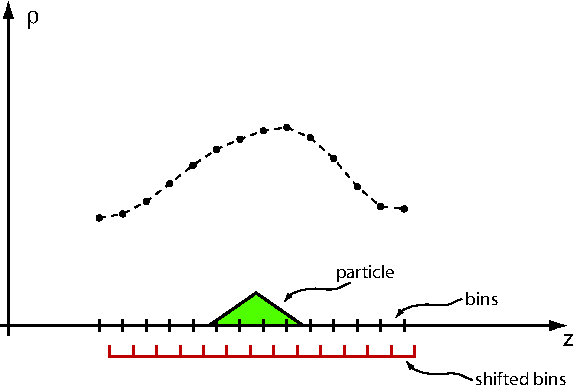
\includegraphics[height=8.4cm]{csr-bin.pdf}
\caption[CSR Calculation]
{The Coherent Synchrotron Radiation kick is calculated by dividing
longitudinally a bunch into a number of bins. To smooth the computed
densities, each particle of the bunch is considered to have a
triangular density distribution.}
\label{f:csr.bin}
\end{figure}

User settable parameters pertenent to the CSR simulation are listed in
\sref{s:csr.params}. Details of how the tracking is implemented is covered
in \sref{s:csr.track}.

\bmad simulates coherent synchrotron radiation using the formalism developed by
Sagan\cite{b:csr}. The total kick received by a particle is divided into two parts: The
space charge (SC) part and the coherent synchrotron radiation (CSR) part. \bmad further
subdivides the SC kick into longitudinal (LSC) and transverse (TSC) parts. Notice that
since the CSR kick is calculated using a 1-dimensional formalism, the CSR kick is strickly
lonitudinal. By definition, the LSC component is the kick that would result if all
particles were traveling in a straight line. The CSR component is what is left when the
LSC kick is subtracted off from the total kick. Generally, the LSC kick is negligible
compared to the CSR kick at large enough particle energies.

Transport through a lattice element involves a beam of particles. The lattice element is
divided up into a number of slices. Transport through a slice is a two step process. The
first step is to give all the particles a kick due to the CSR. The second step is
transport of all particles without any interaction between particles. Note that only the
longitudinal CSR kick is implemented and transverse kicks are ignored.

The particle-particle kick is calculated by dividing the bunch longitudinally into a
number of bins. To smooth the computed bin densities, each particle of the bunch is
considered to have a triangular density distribution as shown in \fig{f:csr.bin}.  The
particle density of a bin is calculated by summing the contribution from all the
particles. The contribution of a given particle to a given bin is calculated from the
overlap of the particle's triangular density distribution with the bin. For the CSR kick,
the density is actually calculated for a second set of staggered bins that have been
offset by 1/2 the bin width with respect to the first set. This gives the density at the
edges of the original set of bins. The density is considered to vary linearly between the
computed density points. For a description of the parameters that affect the CSR
calculation see Section~\sref{s:csr.params}.
 
%-----------------------------------------------------------------   
\section{High Energy Space Charge}
\label{s:space.charge}
\index{CSR|hyperbf}

In tracking, \bmad can simulate the effect of space charge at high energies. To include
this effect, set the \vn{bmad_com[space_charge_on]} parameter (\sref{s:bmad.com}) to True.
The high energy space charge kick is computed assuming a gaussian bunch shape. The high
energy space charge is a separate calculation from the space component of the coherent
synchrotron radiation calculation (\sref{s:csr}).

\chapter{Linear Optics}

%-----------------------------------------------------------------
\section{Coupling and Normal Modes}
\label{s:coupling}
\index{normal mode!Coupling}

The coupling formalism used by \bmad is taken from the paper of Sagan and
Rubin\cite{b:coupling}. The main equations are reproduced here with the notation change
that $\bfA$ and $\bfB$ is replaced by $\bfQ$ and $\bfW$. The reason for this is explained below.

A one--turn map $\bfT(s)$ for the transverse two--dimensional phase space $\bfx = (x, x',
y, y')$ starting and ending at some point $s$ can be written as
  \Begineq
    \bfT = \bfV \, \bfU \, \bfV\inv 
    , \label{tvuv}
  \Endeq 
where $\bfV$ is symplectic, and $\bfU$ is of the form
  \Begineq
    \bfU = 
    \begin{pmatrix}
      \bfQ & \Bf0 \cr 
      \Bf0 & \bfW \cr
    \end{pmatrix}
    . \label{ua00b}
  \Endeq
\index{normal mode!a--mode}
\index{normal mode!b--mode}
Since $\bfU$ is uncoupled the standard Twiss analysis can be performed on the matrices
$\bfQ$ and $\bfW$. The normal modes are labeled $q$ and $w$ and if the one--turn matrix
$\bfT$ is uncoupled then $w$ corresponds to the horizontal mode and $w$ corresponds to the
vertical mode.

The reason why $q$ and $w$ are used here to denote the modes is to avoid confusion with
the \bmad convention of using the labels $a$ and $b$ to represent the same modes
throughout the lattice. At the start of the lattice, by convention, the $a$ mode is the
same as the $q$ mode and the $b$ mode is the same as the $w$ mode. If there is a ``mode
flip'' (see Sagan and Rubin for an explanation of this term) at some spot in the lattice,
the $a$ mode before the mode flip will be the same physical mode after the mode flip (and
similarly for the $b$ mode.  That is, after the mode flip the $a$ mode will be the same as
the $w$ mode and the $b$ mode will be the same as the $q$ mode.

$\bfV$ is written in the form
  \Begineq
    \bfV = 
    \begin{pmatrix}
        \gamma \bfI & \bfC \cr 
        -\bfC^+     & \gamma \bfI \cr
    \end{pmatrix}
    , \label{vgicc1}
  \Endeq
where $\bfC$ is a 2x2 matrix and $+$ superscript 
denotes the symplectic conjugate:
\index{symplectic!conjugate}
  \Begineq
    \bfC^+ = 
    \begin{pmatrix}
       C_{22} & -C_{12} \cr 
      -C_{21} & C_{11} \cr
    \end{pmatrix}
    . \label{ccccc}
  \Endeq
Since we demand that $\bfV$ be symplectic we have the condition
  \Begineq               
    \gamma^2 + \, ||\bfC|| = 1
    , \label{gc1}
  \Endeq
and $\bfV\inv$ is given by
  \Begineq
    \bfV\inv = 
    \begin{pmatrix}
      \gamma \bfI & -\bfC \cr 
      \bfC^+ & \gamma \bfI \cr
    \end{pmatrix}
    . \label{vgicc2}
  \Endeq 
$\bfC$ is a measure of the coupling. 
$\bfT$ is uncoupled if and only if $\bfC = \Bf 0$. 

It is useful to normalize out the $\beta(s)$ variation in the the above
analysis. Normalized quantities being denoted by a bar above them. The
normalized normal mode matrix $\BAR\bfU$ is defined by
  \Begineq
    \BAR\bfU = \bfG \, \bfU \, \bfG\inv
    , \label{ugug}
  \Endeq
Where $\bfG$ is given by 
  \Begineq
    \bfG \equiv 
    \begin{pmatrix}
      \bfG_q & \Bf0 \cr 
      \Bf0 & \bfG_w
    \end{pmatrix}
    , \label{gg00g}
  \Endeq  
with 
  \Begineq
    \bfG_q = 
    \begin{pmatrix}
      \frac{\tstyle 1}{\tstyle \sqrt{\beta_q}} & 0 \cr
      \frac{\tstyle \alpha_q}{\tstyle \sqrt{\beta_q}} & \sqrt{\beta_q}
    \end{pmatrix}
    , \label{g1b0a} 
  \Endeq
with a similar equation for $\bfG_w$. With this definition, the corresponding
$\BAR\bfQ$ and $\BAR\bfW$ (cf.~\Eq{ua00b}) are just rotation matrices.
The relationship between $\bfT$ and $\BAR\bfU$ is 
  \Begineq
    \bfT = \bfG\inv \, \BAR\bfV \, \BAR\bfU \, \BAR\bfV\inv \, \bfG
    , \label{tgvuv}
  \Endeq
where
  \Begineq
    \BAR\bfV = \bfG \, \bfV \, \bfG\inv
    . \label{vgvg}
  \Endeq
Using \Eq{gg00g}, $\BAR\bfV$ can be written in the form
  \Begineq
    \BAR\bfV = 
    \begin{pmatrix}
      \gamma \bfI & \BAR\bfC \cr -\BAR\bfC^+ & \gamma \bfI
    \end{pmatrix}
    , \label{vgicc3}
  \Endeq
with the normalized matrix $\BAR\bfC$ given by
  \Begineq
    \BAR\bfC = \bfG_q \, \bfC \, \bfG_w\inv
    . \label{cgcg}
  \Endeq

The normal mode coordinates ${\bf q} = (q, q', w, w')$ are related to
the laboratory frame via
  \Begineq
    {\bf q} = \bfV\inv \, {\bf x}
    . \label{avx}
  \Endeq 
In particular the normal mode dispersion $\bfeta_q = (\eta_q,
\eta'_q, \eta_w, \eta'_w)$ is related to the laboratory frame
dispersion $\bfeta_x = (\eta_x, \eta'_x, \eta_y, \eta'_y)$ via
  \Begineq
    {\bfeta_q} = \bfV\inv \, {\bfeta_x}
    . \label{etaavx}
  \Endeq 
When there is no coupling ($\bfC = 0$), $\bfeta_q$ and $\bfeta_x$ are
equal to each other.

%-----------------------------------------------------------------
\section{Dispersion Calculation}
\label{s:dispersion}
\index{dispersion|hyperbf}

The dispersion ($\eta$) and the dispersion derivative ($\eta'$) are 
defined by the equations
\begin{align}
  \eta_x(s) &\equiv \left. \frac{dx}{dp_z} \right|_s \comma \qquad
    \eta'_x(s) \equiv \left. \frac{d\eta_x}{ds} \right|_s
    = \left. \frac{dx'}{dp_z} \right|_s \CRNO
  \eta_y(s) &\equiv \left. \frac{dy}{dp_z} \right|_s \comma \qquad
    \eta'_y(s) \equiv \left. \frac{d\eta_y}{ds} \right|_s
    = \left. \frac{dy'}{dp_z} \right|_s \\
  \eta_z(s) &\equiv \left. \frac{dz}{dp_z} \right|_s \nonumber
\end{align}

Given the dispersion at a given point, the dispersion at some other
point is calculated as follows: Let $\Bf r = (x, p_x, y, p_y, z, p_z)$
be the reference orbit, around which the dispersion is to be
calculated. Let $\bfV$ and $\bf M$ be the zeroth and first order
components of the transfer map between two points labeled 1 and 2:
\Begineq
  \Bf r_2 = \bfM \, \Bf r_1 + \bfV
  \label{rmrv}
\Endeq
Define the dispersion vector $\bfeta$ by
\Begineq
  \bfeta = 
  \left( 
    \eta_x, \eta'_x \, (1 + p_z), \eta_y, \eta'_y \, (1 + p_z), \eta_z, 1
  \right)
\Endeq
Differentiating \Eq{rmrv} with respect to energy, 
the dispersion at point 2 in terms of the dispersion at point 1 is
\Begineq
  \bfeta_2 = \left[ \frac{dp_{z2}}{dp_{z1}} \right]^{-1} \, 
    \left[ \bfM \, \bfeta_1 \right] + \bfV_\eta 
    \label{eppmev}
\Endeq
where
\Begineq
  \bfV_\eta = \left[ \frac{dp_{z2}}{dp_{z1}} \right]^{-1} \, 
  \frac{1}{1 + p_{z1}}
  \left(
  \begin{array}{c}
    M_{12} \, p_{x1} + M_{14} \, p_{y1} \\
    M_{22} \, p_{x1} + M_{24} \, p_{y1} \\
    M_{32} \, p_{x1} + M_{34} \, p_{y1} \\
    M_{42} \, p_{x1} + M_{44} \, p_{y1} \\
    M_{52} \, p_{x1} + M_{54} \, p_{y1} \\
    M_{62} \, p_{x1} + M_{64} \, p_{y1} \\
  \end{array}
  \right)
  -
  \left(
  \begin{array}{c}
    0 \\
    \frac{p_{x2}}{1 + p_{z2}} \\
    0 \\
    \frac{p_{y2}}{1 + p_{z2}} \\
    0 \\
    0 
  \end{array}
  \right)
\Endeq
The sixth row of the matrix equation gives $dp_{z1}/dp_{z2}$. 
Explicitly
\Begineq
  \frac{dp_{z2}}{dp_{z1}} =
  \sum_{i=1}^6 M_{6i} \, \eta_{1i} + 
  \frac{M_{62} \, p_{x1} + M_{64} \, p_{y1}}{1 + p_{z1}}
\Endeq
For everything except \vn{RFcavity} and \vn{Lcavity} elements, 
$dp_{z2}/dp_{z1}$ is 1.

For a non-circular machine, there are two ways one can imagine
defining the dispersion: Either with respect to changes in energy at
the beginning of the machine or with respect to the local change in
energy at the point of measurement. The former definition will be
called ``non-local dispersion'' and the latter definition will be
called ``local dispersion''. For a circular machine, local dispersion
is always used.  The dispersion defined in the above equations, which
is what \bmad uses in calculations, is the local dispersion. The
non-local dispersion $\wt\bfeta(s_1)$ at some point $s_1$ is related
to the local dispersion $\bfeta(s_1)$ via
\Begineq
  \wt\bfeta(s_1) = \frac{dp_{z1}}{dp_{z0}} \, \bfeta(s_1)
\Endeq
where $s_0$ is the beginning of the machine.

For a non-circular machine, there are advantages and disadvantages to
using either local or non-local dispersion. Local dispersion has the
problem that $dp_{z2}/dp_{z1}$ in \Eq{eppmev} may go through zero at a
point producing infinite dispersions at that point. The non-local
dispersion has the merit of reflecting what one would measure if the
starting energy of the beam is veried. The local dispersion, on the
other hand, reflects the correlations between the particle energy and
particle position within a beam.


\chapter{Taylor Maps}

%-----------------------------------------------------------------
\section{Taylor Maps}
\label{s:taylor.phys}
\index{taylor map|hyperbf}
\index{symplectic integration}

A transport map ${\cal M}: {\cal R}^6 \rightarrow {\cal R}^6$ through
an element or a section of a lattice is a function that maps the
starting phase space coordinates $\Bf r(\In)$ to the ending
coordinates $\Bf r(\Out)$
\begin{equation}
  \Bf r(\Out) = {\cal M} \, (\delta \bfr)
\end{equation}
where
\Begineq
  \delta \bfr = \bfr(\In) - \bfr_\Ref
\Endeq
$\bfr_\Ref$ is the reference orbit at the start of the map around which the map is
made. In many cases the reference orbit is the zero orbit. For a storage ring, the closed
orbit is commanly used for the reference orbit.

${\cal M}$ in the above equation is made up of six functions ${\cal M}_i: {\cal R}^6
\rightarrow {\cal R}$. Each of these functions maps to one of the $r(\Out)$
coordinates. Each of these functions can be expanded in a Taylor series and truncated at
some order. Each Taylor series is in the form
\Begineq
  r_i(\Out) = \sum_{j = 1}^N \, C_{ij} \, \prod_{k = 1}^6 \, (\delta r_k)^{e_{ijk}}
  \label{rcr}
\Endeq
Where the $C_{ij}$ are coefficients and the $e_{ijk}$ are integer exponents.
The order of a given term associated with index $i,j$ is the sum over the exponents
\Begineq
  \text{order}_{ij} = \sum_{k = 1}^6 e_{ijk} 
\Endeq
The order of the entire map is the order at which the map is truncated.

The standard \bmad routine for printing a Taylor map might produce something 
like this: 
\begin{example}
   Taylor Terms:
   Out      Coef             Exponents          Order       Reference
   --------------------------------------------------
    1:     -0.600000000000   0  0  0  0  0  0       0       0.200000000
    1:      1.000000000000   1  0  0  0  0  0       1
    1:      0.145000000000   2  0  0  0  0  0       2
   --------------------------------------------------
    2:     -0.185000000000   0  0  0  0  0  0       0       0.000000000
    2:      1.300000000000   0  1  0  0  0  0       1
    2:      3.800000000000   2  0  0  0  0  1       3
   --------------------------------------------------
    3:      1.000000000000   0  0  1  0  0  0       1       0.100000000
    3:      1.600000000000   0  0  0  1  0  0       1
    3:    -11.138187077310   1  0  1  0  0  0       2
   --------------------------------------------------
    4:      1.000000000000   0  0  0  1  0  0       1       0.000000000
   --------------------------------------------------
    5:      0.000000000000   0  0  0  0  0  0       0       0.000000000
    5:      0.000001480008   0  1  0  0  0  0       1
    5:      1.000000000000   0  0  0  0  1  0       1
    5:      0.000000000003   0  0  0  0  0  1       1
    5:      0.000000000003   2  0  0  0  0  0       2
   --------------------------------------------------
    6:      1.000000000000   0  0  0  0  0  1       1       0.000000000
\end{example}
Each line in the example represents a single \vn{Taylor term}. The
Taylor terms are grouped into 6 \vn{Taylor series}. There is one
series for each of the output phase space coordinate. The first
column in the example, labeled ``out'', (corresponding to the $i$
index in \Eq{rcr}) indicates the Taylor series: $1 = x(out)$, $2 =
p_x(out)$, etc. The 6 exponent columns give the $e_{ijk}$ of
\Eq{rcr}. In this example, the second Taylor series (\vn{out} = 2),
when expressed as a formula, would read:
\Begineq
  p_x(out) = -0.185 + 1.3 \, \delta p_x + 3.8 \, \delta x^2 \, \delta p_z
\Endeq

\index{taylor map!reference coordinates}
The reference column in the above example shows the input coordinates around
which the Taylor map is calculated. In this case, the reference
coordinates where 
\Begineq
  (x, p_x, y, p_y, z, p_z)_{ref} = (0.2, 0, 0.1, 0, 0, 0, 0)
\Endeq
The choice of the reference point will affect the values of the
coefficients of the Taylor map. As an example, consider the 1-dimension map
\Begineq
  x(out) = A \, \sin(k \, \delta x)
\Endeq
Then a Taylor map to 1\St order is
\Begineq
  x(out) = c_0 + c_1 \, \delta x
\Endeq
where
\begin{align}
  c_1 &= A \, k \, \cos(k \, x_{\text{ref}}) \\
  c_0 &= A \, \sin(k \, x_{\text{ref}})
\end{align}

%-----------------------------------------------------------------
\section{Spin Taylor Map}
\label{s:spin.map}
\index{spin taylor map}

A Taylor map that fully describes spin and orbital motion, would
consist of nine Taylor series (six for the orbital phase space
variables and three for the spin components) and each Taylor series
would be a polynomial in nine variables.

To simplify things, \bmad assumes that the effect on the orbital phase
space due to the spin orientation is negligible. That is, Stern-Gerlach
effects are ignored. With this assumption, the orbital part of the map
is only dependent on the six orbital variables. Furthermore, 
the three spin Taylor series are linear in the spin coordinates
and can be cast into matrix form:
\Begineq
  S_i(\Out) = \sum_{j} \Bf\Lambda_{ij}(\bfr(\In) - \bfr_\Ref) \, S_j(\In)
\Endeq
where $\Bf S = (s_x, s_y, s_z)$ is the spin and $\Bf\Lambda_{ij}$ are
Taylor series that are only dependent upon the orbit coordinates. The
proof of this assertion is derived from the
Thomas-Bargmann-Michel-Telegdi equation (\sref{tbmt}). Since the
orbital coordinates are assumed independent of the spin, the TBMT
equation is linear in the spin and thus the transport can be described
by a matrix. Furthermore, since the spin magnitude is an invarient,
for given initial orbit coordinates, The $\Bf\Lambda_{ij}$ matrix,
evaluated for some given initial orbital starting point, must just
represent a rotation about some axis. While use of the $\Bf\Lambda$
matrix increases the number of Taylor series needed from 9 to 15, all
the series are now only dependent on the six orbit coordinates.

The standard \bmad routine for printing a spin Taylor map will produce
something like this:
\begin{example}
  Spin Taylor Terms:
  Out      Coef_Sx         Coef_Sy         Coef_Sz      Exponents           Order
  -------------------------------------------------------------------------------
  Sx:      0.99757886     -0.02372254     -0.06537314   0  0  0  0  0  0        0
  Sx:      0.04802411      0.22401654      0.65154583   1  0  0  0  0  0        1
  Sx:      0.07391383      3.77338795     -0.24137562   0  1  0  0  0  0        1
  Sx:      0.00008802     -0.17584738      0.06515458   0  0  1  0  0  0        1
  Sx:      0.01148244     -0.20322945      0.24896717   0  0  0  1  0  0        1
  Sx:     -0.00457076     -0.22322148      0.01125358   0  0  0  0  0  1        1
  -------------------------------------------------------------------------------
  Sy:     -0.02460178      0.75885811     -0.65079114   0  0  0  0  0  0        0
  Sy:      0.25039365     -0.04801091     -0.06544895   1  0  0  0  0  0        1
  Sy:     -3.02631629     -0.07739091      0.02416143   0  1  0  0  0  0        1
  Sy:      0.17584738      0.00008802     -0.00654489   0  0  1  0  0  0        1
  Sy:      0.47579058      1.59361755      1.84025908   0  0  0  1  0  0        1
  Sy:      0.13046518     -0.46155512     -0.54313051   0  0  0  0  0  1        1
  -------------------------------------------------------------------------------
  Sz:      0.06504736      0.65082378      0.75643719   0  0  0  0  0  0        0
  Sz:     -0.64180483      0.06414595      0.00000000   1  0  0  0  0  0        1
  Sz:     -2.27815007      0.22777762     -0.00007328   0  1  0  0  0  0        1
  Sz:      0.06515785     -0.00651227      0.00000000   0  0  1  0  0  0        1
  Sz:      0.00385332     -1.86555986      1.60475990   0  0  0  1  0  0        1
  Sz:      0.11944181      0.53003513     -0.46630288   0  0  0  0  0  1        1
\end{example}
The reference orbit is seen by printing the orbital part of the map.

%-----------------------------------------------------------------
\section{Symplectification}
\label{s:symp.method}
\index{symplectification}

If the evolution of a system can be described using a Hamiltonian then
it can be shown that the linear part of any transport map (the Jacobian)
must obey the symplectic condition. If a matrix $\Bf M$ is not symplectic,
Healy\cite{b:healy} has provided an elegant method for finding a symplectic 
matrix that is ``close'' to $\Bf M$. The procedure is as follows:
From $\Bf M$ a matrix $\bfV$ is formed via
\begin{equation}
  \bfV = \Bf S (\Bf I - \Bf M)(\Bf I + \Bf M)^{-1} 
  \label{e:vsimi}
\end{equation}
where $\Bf S$ is the matrix
\Begineq
  \Bf S = 
  \begin{pmatrix} 
      0 &  1 &  0 &  0 &  0 &  0 \cr
     -1 &  0 &  0 &  0 &  0 &  0 \cr
      0 &  0 &  0 &  1 &  0 &  0 \cr
      0 &  0 & -1 &  0 &  0 &  0 \cr
      0 &  0 &  0 &  0 &  0 & -1 \cr
      0 &  0 &  0 &  0 & -1 &  0 \cr
  \end{pmatrix}
  \label{s0100}
\Endeq
$\bfV$ is symmetric if and only if $\Bf M$ is symplectic. In any case,
a symmetric matrix $\Bf W$ near $\bfV$ can be
formed via
\begin{equation}
  \Bf W = \frac{\bfV + \bfV^t}{2}
\end{equation}
A symplectic matrix $\Bf F$ is now obtained by inverting \eq{e:vsimi}
\Begineq
  \Bf F = (\Bf I + \Bf S \Bf W) (\Bf I - \Bf S \Bf W)^{-1}
\Endeq

%-----------------------------------------------------------------
\section{Map Concatenation and Feed-Down}
\label{s:map.concat}

\index{taylor map!feed-down}
Of importance in working with Taylor maps is the concept of
\vn{feed-down}.  This is best explained with an example. To keep the
example simple, the discussion is limited to one phase space
dimension so that the Taylor maps are a single Taylor series. Take the
map $M_1$ from point 0 to point 1 to be
\Begineq
  M_1: x_1 = x_0 + 2
  \label{xx2}
\Endeq
and the map $M_2$ from point 1 to point 2 to be
\Begineq
  M_2: x_2 = x_1^2 + 3 \, x_1
  \label{xx3x}
\Endeq
Then concatenating the maps to form the map $M_3$ from point 0 to point 2
gives
\Begineq
  M_3: x_2 = (x_0 + 2)^2 + 3 (x_0 + 2) = x_0^2 + 7 \, x_0 + 10
  \label{xx23x2}
\Endeq
However if we are evaluating our maps to only 1\St order the map $M_2$
becomes
\Begineq
  M_2: x_2 = 3 \, x_1
\Endeq
and concatenating the maps now gives
\Begineq
  M_3: x_2 = 3 (x_0 + 2) = 3 \, x_0 + 6
  \label{x3x23}
\Endeq
Comparing this to \Eq{xx23x2} shows that by neglecting the 2\Nd order
term in \Eq{xx3x} leads to 0\Th and 1\St order errors in
\Eq{x3x23}. These errors can be traced to the finite 0\Th order term in
\Eq{xx2}. This is the principal of feed--down: Given $M_3$ which is a map
produced from the concatenation of two other maps, $M_1$, and $M_2$
\Begineq
  M_3 = M_2(M_1)
\Endeq
Then if $M_1$ and $M_2$ are correct to n\Th order, $M_3$ will also be
correct to n\Th order as long as $M_1$ has no constant (0\Th order)
term. [Notice that a constant term in $M_2$ does not affect the
argument.]  What happens if we know there are constant terms in our
maps? One possibility is to go to a coordinate system where the
constant terms vanish. In the above example that would mean using the
coordinate $\widetilde x_0$ at point 0 given by
\Begineq
  \widetilde x_0 = x_0 + 2
\Endeq
\index{symplectic integration}

%-----------------------------------------------------------------
\section{Symplectic Integration}
\label{s:symp.integ}

Symplectic integration, as opposed to concatenation, never has
problems with feed--down. The subject of symplectic integration is too
large to be covered in this guide. The reader is referred to the book
``Beam Dynamics: A New Attitude and Framework'' by \'Etienne
Forest\cite{b:forest}. A brief synopsis: Symplectic integration uses
as input 1) The Hamiltonian that defines the equations of motion, and
2) a Taylor map $M_1$ from point 0 to point 1. Symplectic integration
from point 1 to point 2 produces a Taylor map $M_3$ from point 0 to
point 2. Symplectic integration can produce maps to arbitrary
order. In any practical application the order $n$ of the final map is
specified and in the integration procedure all terms of order higher
than $n$ are ignored. If one is just interested in knowing the final
coordinates of a particle at point 2 given the initial coordinates at
point 1 then $M_1$ is just the constant map
\Begineq
  M_1: x_1 = c_i
\Endeq
where $c_i$ is the initial starting point. The order of the
integration is set to 0 so that all non--constant terms are
ignored. The final map is also just a constant map
\Begineq
  M_3: x_2 = c_f
\Endeq
If the map from point 1 to point 2 is desired then the map $M_1$ is
just set to the identity map
\Begineq
  M_1: x_1 = x_0
\Endeq
In general it is impossible to exactly integrate any non--linear
system. In practice, the symplectic integration is achieved by slicing
the interval between point 1 and point 2 into a number of (generally
equally spaced) slices. The integration is performed, slice step by
slice step. This is analogous to integrating a function by evaluating
the function at a number of points. Using more slices gives better
results but slows down the calculation. The speed and accuracy of the
calculation is determined by the number of slices and the \vn{order}
of the integrator. The concept of integrator order can best be
understood by analogy by considering the trapezoidal rule for
integrating a function of one variable:
\Begineq
  \int_{y_a}^{y_b} f(y) \, dy = 
  h \left[ \frac{1}{2} f(y_a) + \frac{1}{2} f(y_b) \right] +
  o(h^3 \, f^{(2)})
\Endeq
In the formula $h = y_b - y_a$ is the slice width. $0(h^3 \, f^{(2)})$
means that the error of the trapezoidal rule scales as the second
derivative of $f$. Since the error scales as $f^{(2)}$ this is an
example of a second order integrator. To integrate a function between
points $y_1$ and $y_N$ we slice the interval at points $y_2 \ldots y_{N-1}$
and apply the trapezoidal rule to each interval. Examples of higher
order integrators can be found, for example, in Numerical
Recipes\cite{b:nr}. The concept of integrator order in symplectic
integration is analogous. 

The optimum number of slices is determined by the smallest number that
gives an acceptable error. The slice size is given by the \vn{ds_step}
attribute of an element (\sref{s:integ}).  Integrators of higher order
will generally need a smaller number of slices to achieve a given
accuracy. However, since integrators of higher order take more time
per slice step, and since it is computation time and not number of
slices which is important, only a measurement of error and calculation
time as a function of slice number and integrator order will
unambiguously give the optimum integrator order and slice width.  In
doing a timing test, it must be remembered that since the magnitude of
any non-linearities will depend upon the starting position, the
integration error will be dependent upon the starting map $M_1$. \bmad
has integrators of order 2, 4, and 6 (\sref{s:integ}). Timing tests
performed for some wiggler elements (which have strong nonlinearities)
showed that, in this case, the 2\Nd order integrator gave the fastest
computation time for a given accuracy. However, the higher order
integrators may give better results for elements with weaker
nonlinearities.

\chapter{Tracking of Charged Particles}
\label{c:charged.track}

\bmad can track both charged particles and X-rays. This chapter deals
with charged particles and X-rays are handled in
chapter~\sref{c:xray.track}.

For tracking and transfer map calculations (here generically called
``tracking''), \bmad has various methods that can be applied to a
given element (Cf. Chapter~\sref{c:methods}). This chapter discusses
the \vn{bmad_standard} calculation that is the default for almost all
element types and the \vn{symp_lie_bmad} calculation that does
symplectic integration.

Generally, it will be assumed that tracking is in the forward direction.

%-----------------------------------------------------------------
\section{Relative Versus Absolute Time Tracking}
\label{s:rf.time}

\index{relative time tracking}\index{absolute time tracking}
\index{lcavity}\index{rfcavity}\index{em_field}
Unlike other elements, the kick given a particle going through an
\vn{lcavity}, \vn{rfcavity}, or possibly an \vn{em_field} element
depends upon the time that the particle enters the element relative to
some ``RF clock''. \bmad has two modes for calculating this time
called ``\vn{relative time tracking}'' and ``\vn{absolute time
tracking}''. The switch to set the type of tracking for a lattice is
\vn{parameter[absolute_time_tracking]} (\sref{s:param}).

The phase of the RF, $\phi_\text{rf}$, is determined by
\Begineq
  \phi_\text{rf} = \phi_\text{t} + \phi_\text{ref}
\Endeq
where $\phi_\text{t}$ is the part of the phase that depends upon
the time $t$ and $\phi_\text{ref}$ is a fixed phase offset (generally set
in the lattice file) and independent of the particle coordinates.

With \vn{relative time tracking}, which \bmad uses by default, the
value of $\phi_\text{t}$ at the entrance to an element is determined
by by the phase space $z$ coordinate (\sref{s:phase.space}):
\Begineq
  \phi_\text{t}(s) = \frac{-z(s) \, f_\text{rf}}{(\beta \, c)}
  = f_\text{rf} \, (t(s) - t_0(s))
\Endeq
where $f_\text{rf}$ is the RF frequency, and $t_0$ is the reference
time (\sref{s:phase.space}).

With \vn{absolute time tracking}, the RF phase at the entrance to the
cavity is determined by
\Begineq
  \phi_\text{t}(s) = f_\text{rf} \, (t(s) - t_\text{e0})
\Endeq
where $t_\text{e0}$ is the \vn{element reference time}. The element
reference time is, by definition, equal to $t_{0}(s)$ when $s$ is the
distance from the beginning of the lattice to the entrance of the RF
element. 

To understand the distinction between $t_0$ and $t_\text{e0}$,
consider a particle traveling on the reference orbit along side the
reference particle in a circular ring with one RF cavity. This
particle always has $z = 0$ and thus, with \vn{relative time
tracking}, $\phi_t$ will always be zero at the entrance to the cavity.
With \vn{absolute time tracking}, the particle, on the first turn,
will have $\phi_t$ equal to zero. However, on subsequent turns the
phase will increase by $f_\text{rf} \, t_\text{C}$ on each turn where
$t_\text{C}$ is the revolution time. If $f_\text{rf}$ is some multiple
of the revolution harmonic, the RF phase with absolute vs relative
time tracking will be some multiple of $2 \, \pi$ and thus RF kick
given the particle will be the same in both cases. However, if the RF
frequency is not some multiple of the revolution harmonic, there will
be a difference in the RF kicks (except for the kick on the first
turn).

There are advantages and disadvantages to using either relative or
absolute time tracking. Absolute time tracking is more correct since
RF cavities are in reality synced to some clock. The problem with
absolute time tracking is that the transfer map through the cavity is
now a function of time and therefore is a function of $z$ and the turn
number.  This complicates lattice analysis. For example, standard
element transfer maps use phase space coordinates so with absolute
time tracking, one has a different map for each turn.

With relative time tracking the transfer map problem is swept under
the rug. The penalty for using relative time tracking is that results
can be unphysical. For example, the closed orbit is essentially
independent of the RF frequency. From a different angle this can be
viewed as a good feature since if one is only interested in, say,
calculating the Twiss parameters, it can be an annoyance to have to
worry that the ring one has constructed have a length that is exactly
conmensurate with the RF frequency and it is potentially confusing to
see non-zero closed orbits when one is not expecting it.

The above discussion is limited to the cavity fundamental mode.
Long-range wake fields, on the other hand, cannot be synchronized to
the $z$ coordinate since, in general, their frequencies are not
commensurate with the fundamental mode frequency. For simulating the
long-range wakes, the kick is thus, by necessity, tied to the absolute
time. The exception is that a wake associated with the fundamental
mode (that is, has the same frequency as the fundamental mode) will
always use relative time if the fundamental is using relative time and
vice versa.

Do not confuse absolute time tracking with the \vn{time_runge_kutta}
tracking method (\sref{s:tkm}). The \vn{time_runge_kutta} method uses
time as the independent variable instead of $z$. Absolute time
tracking just means that the RF phase is dependent upon the time
instead of $z$. It is perfectly possible to use absolute time
tracking with code that uses $z$ as the independent variable.

%-------------------------------------------------------------------------
%-------------------------------------------------------------------------
\section{Element Coordinate System}
\label{s:ele.coords}

\index{element coordinates}
The general procedure for tracking through an element makes use of
\vn{element reference} coordinates (also called just \vn{element}
coordinates). Without any offsets, pitches or tilt (\sref{s:offset}), henceforth
called ``misalignments'', the \vn{element} coordinates are the same
as the \vn{laboratory reference} coordinates (or simply \vn{laboratory}
coordinates) (\sref{s:ref}). The \vn{element} coordinates stay fixed
relative to the element. Therefore, if the element is misaligned, the
\vn{element coordinates} will follow as the element shifts in the
laboratory frame as shown in \fig{f:ele.coord}.

Tracking a particle through an element is a three step process:
\begin{enumerate}
\item
At the entrance end of the element, transform from the \vn{laboratory}
coordinates to the entrance \vn{element} coordinates.
\item
Track through the element ignoring any misalignments. 
\item
At the exit end of the element, transform from the exit \vn{element}
reference frame to the \vn{laboratory} reference frame.
\end{enumerate}

The transformation between \vn{laboratory} and \vn{element} reference
frames is given in \sref{s:straight.mis} and \sref{s:bend.mis}.

%-------------------------------------------------------------------------

\begin{figure}[tb]
  \centering
  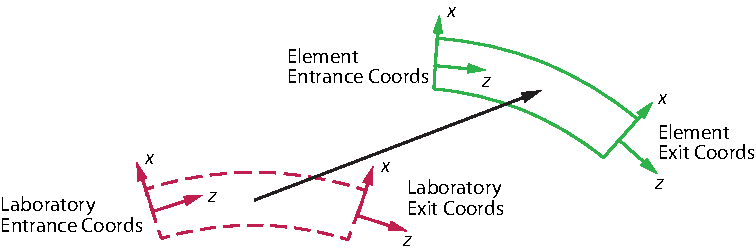
\includegraphics[width=5in]{coord-offset.pdf}
  \caption[Element Coordinate System.]
  {
\vn{Element} coordinates are coordinates attached to the physical
element (solid green outline). The \vn{laboratory} coordinates are
fixed at the nominal position of the element (red dashed outline).
  }
  \label{f:ele.coord}.
\end{figure}

%-------------------------------------------------------------------------
\section{Hamiltonian}
\label{s:mag.hamiltonian}
The time dependent Hamiltonian $H_t$ in the curvilinear coordinate system shown
in \fig{f:local.coords} is (\cite{b:ruth})
\Begineq
  H_t = \wt\psi + \left[ \left( \frac{p_s - a_s}{1 + g\, x} \right)^2 + \wt m^2 + 
  (p_x - a_x)^2 + (p_y - a_y)^2 \right]^{1/2}
\Endeq
where $(p_x, p_y, p_s/(1+gx))$ are the momentum normalized by $P_0$,
$\rho$ being the local radius of curvature of the reference particle,
and $\wt m$, $\Bf a$ and $\wt\psi$ are the normalized mass, vector, and scalar
potentials:
\Begineq
  \wt m = \frac{m \, c^2}{c \, P_0} \qquad
  \left( a_x, a_y, \frac{a_s}{1+g \, x} \right) = \frac{q \, \Bf A}{P_0 \, c} \qquad 
  \wt\psi(x,y,z) = \frac{q \, \psi}{P_0 \, c}
  \label{mmccp}
\Endeq
In terms of the normalized velocities $\beta_x$, $\beta_y$, the canonical momentum are
\Begineq
  p_x = \frac{m \, c^2}{P_0 \, c} \, \beta_x + a_x, \qquad 
  p_y = \frac{m \, c^2}{P_0 \, c} \, \beta_y + a_y
  \label{pmc2pc}
\Endeq

The $s$-dependent Hamiltonian is obtained from $H_t$ by solving for
$-p_s$ and using a contact transformation to convert to \bmad
coordinates (\sref{s:phase.space}). For particles propagating in the
positive $s$ direction, the $s$-dependent Hamiltonian is, assuming
$\wt\psi$ is zero
\Begineq
  H \equiv H_s = -(1 + g \, x) \sqrt{(1 + p_z)^2 - (p_x - a_x)^2 - (p_y - a_y)^2} - 
  a_s + \frac{1}{\beta_0} \, \sqrt{(1+p_z)^2 + \wt m^2}
  \label{h1gx1}
\Endeq
where $\beta_0$ is the reference velocity and the equality $(1 +
p_z)^2 = (E/c\, P_0)^2 - \wt m^2$ has been used. The last term on the
RHS of \Eq{h1gx1} accounts for the fact that the \bmad canonical $z$
(\Eq{zbctt}) has an ``extra'' term $\beta \, c \, t_0$ so that \bmad
canonical $z$ is with respect to the reference particle's $z$.

The equations of motion are
\begin{equation}
  \frac{dq_i}{ds} = \frac{\partial H}{\partial p_i} \qquad
  \frac{dp_i}{ds} = -\frac{\partial H}{\partial q_i}
  \label{rshp}
\end{equation}

\label{paraxial approximation} Without an electric field, $\psi$ is zero. Assuming a
non-curved coordinate system ($g = 0$), and using the paraxial approximation (which
expands the square root in the Hamiltonian assuming the transverse momenta are small)
(\sref{s:phase.space}), \Eq{h1gx1} becomes
\Begineq
  H = \frac{(p_x - a_x)^2}{2 (1 + p_z)} + \frac{(p_y - a_y)^2}{2 (1 + p_z)} - 
  (1 + g \, x) \, (1 + p_z) - a_s +   \frac{1}{\beta_0} \, \sqrt{(1+p_z)^2 + \wt m^2}
  \label{hpapa}
\Endeq

Once the transverse trajectory has been calculated, the longitudinal position
$z_2$ at the exit end of an element is obtained from symplectic
integration of \Eq{hpapa}
\Begineq
  z_2 = z_1 - \frac{1}{2 (1 + p_{z1})^2} \int \! ds \, 
  \left[ (p_x - a_x)^2 + (p_y - a_y)^2 \right] - \int \! ds \, g \, x
  \label{zz121p}
\Endeq
where $z_1$ is the longitudinal position at the entrance end of the element.
Using the equations of motion \Eqs{rshp} this can also be rewritten as
\Begineq
  z_2 = z_1 - \frac{1}{2} \int \! ds \, 
  \left[ \left( \frac{dx}{ds} \right)^2 + \left( \frac{dy}{ds} \right)^2 \right] - 
  \int \! ds \, g \, x
  \label{zz12sx}
\Endeq

For some elements, \vn{bmad_standard} uses a truncated Taylor map for
tracking.  For elements without electric fields where the particle
energy is a constant, the transfer map for a given coordinate $r_i$
may be expanded in a Taylor series
\Begineq
  r_{i,2} \rightarrow m_i + \sum_{j = 1}^4 m_{ij} \, r_{j,1} + 
  \sum_{j = 1}^4 \sum_{k = j}^4 m_{ijk} \, r_{j,1} \, r_{k,1} + \ldots
\Endeq
where the map coefficients $m_{ij\cdots}$ are functions of $p_z$.  For
linear elements, the transfer map is linear for the transverse
coordinates and quadratic for $r_i = z$.

Assuming mid--plane symmetry of the magnetic field, so
that $a_x$ and $a_y$ can be set to zero\cite{b:madphysics}, The vector
potential up to second order is (cf.~\Eq{byx0b})
\Begineq
  a_s = -k_0 \left( x - \frac{g \, x^2}{2 (1 + g\, x)} \right) -
  \frac{1}{2} k_1 \left( x^2 - y^2 \right)
  \label{akxgx}
\Endeq

For backwards propagation, where particle are traveling in the $-\Bf
s$ direction and where $p_s$ is negative, solving for $p_s$ involves
using a different part of the square root branch. There is also an
overall negative sign coming from switching from using $s$ as the
independent variable to $\wt s \equiv -s$ as the independent
variable. the Hamiltonian $H_{\wt s}$ is then
\Begineq
  H_{\wt s} = -(1 + g \, x) \sqrt{(1 + p_z)^2 - (p_x - a_x)^2 - (p_y - a_y)^2} + 
  a_s + \frac{1}{\beta_0} \, \sqrt{(1+p_z)^2 + \wt m^2}
\Endeq

%---------------------------------------------------------------------------------
%---------------------------------------------------------------------------------
\section{Symplectic Integration}
\label{s:symp.track}
\index{symplectic integration}

Using \Eq{hpapa} the Hamiltonian is written in the form
\Begineq
  H = H_x + H_y + H_z
\Endeq
where
\begin{equation}
  H_x = \frac{(p_x - a_x)^2}{2 (1 + \delta)}, \qquad
  H_y = \frac{(p_y - a_y)^2}{2 (1 + \delta)}, \qquad
  H_s = - a_s 
\end{equation}

For tracking, the element is broken up into a number of slices set by
the element's \vn{ds_step} attribute. For each slice, the tracking
uses a quadratic symplectic integrator $I$:
\Begineq
  I = T_{s/2} \; I_{x/2} \; I_{y/2} \; I_s \; I_{y/2} \; I_{x/2} \; T_{s/2}
\Endeq
$T_{s/2}$ is just a translation of the $s$ variable:
\Begineq
  s \rightarrow s + \frac{ds}{2}
\Endeq
And the other integrator components are
\begin{align}
  I_{x/2} &= \exp \left( : -\frac{ds}{2} H_x : \right) \CRNO
  I_{y/2} &= \exp \left( : -\frac{ds}{2} H_y : \right) \\
  I_{s}   &= \exp \left( : -ds \, H_s : \right) \nonumber
\end{align}
The evaluation of $I_{x/2}$ and $I_{y/2}$ is tricky since it involves both transverse
position and momentum variables. The trick is to split the integration into three parts.
For $I_{x/2}$ this is
\begin{align}
  I_{x/2} &= \exp \left( : -\frac{ds}{2} \frac{(p_x - A_x)^2}{2 (1 + \delta)} : \right) \CRNO
  &= \exp \left( : -\int A_x \, dx : \right) \,
     \exp \left( : -\frac{ds}{2} \frac{p_x^2}{2 (1 + \delta)} : \right) \,
     \exp \left( : \int A_x \, dx : \right)
  \label{ids2}
\end{align}
With an analogous expression for $I_{y/2}$.

\index{quadrupole}\index{sextupole}\index{wiggler}
For magnetic elements that do not have longitudinal fields
(quadrupoles, sextupoles, etc.), $a_x$ and $a_y$ can be taken to be
zero (cf.~\Eq{akxgx}).

\index{lcavity}\index{rfcavity}
For \vn{lcavity} and \vn{rfcavity} elements, the vector potential is computed from
\Eq{aiew}.

%-----------------------------------------------------------------   
\section{Spin Dynamics}   
\label{s:spin.dyn}
\index{spin|hyperbf}   

\textit{\large [Spin dynamics initially developed by Jeff Smith]}

The classical spin vector $\Bf S$ is described in the local reference
frame (\sref{s:ref}) by a modified Thomas-Bargmann-Michel-Telegdi
(T-BMT) equation\cite{b:spin}
\Begineq
  \frac{\mathrm{d}}{\mathrm{d}s} \Bf S = 
  \left\{ \frac{(1+\Bf r_t \dotproduct \bfg)}{c \, \beta_z} \, 
  \left( {\pmb\Omega}_{BMT} + {\pmb\Omega}_{EDM} \right) - 
  \bfg \times \bfhat z \right\} \times \mathbf{S}
  \label{tbmt}
\Endeq
where $\bfg$ is the bend curvature function which points away from the center of curvature
of the particle's reference orbit (see \fig{f:local.coords}), $\Bf r_t = (x, y)$ are the
transverse coordinates, $c \, \beta_z$ is the longitudinal component of the velocity, and
$\bfhat z$ is the unit vector in the $z$-direction. $\pmb\Omega_{BMT}$ is the usual T-BMT
precession vector due to the particle's magnetic moment and $\pmb\Omega_{EDM}$ is the
precession vector due to a finite electric dipole moment (EDM) \cite{b:silenko}
\begin{align}
  {\pmb\Omega}_{BMT} (\mathbf{r,P},t) &= 
    - \frac{q}{m \, c} \left[ 
    \left(\frac{1}{\gamma} + G \right) \, c \, \Bf B -
    \frac{G \, \gamma \, c}{1 + \gamma} \, ( \bfbeta \dotproduct \Bf B ) \, \bfbeta -
    \left( G + \frac{1}{1 + \gamma} \right) \, \mathbf{\bfbeta \times  E} 
    \right] \\
  &= - \frac{q}{m \, c} \left[ 
    \left( \frac{1}{\gamma} + G \right) \, c \, \Bf B_{\perp} +
    \frac{(1 + G) \, c}{\gamma} \, \Bf B_\parallel -
    \left( G + \frac{1}{1 + \gamma} \right) \mathbf{\bfbeta \times E} 
    \right] \nonumber
\end{align}
and
\Begineq
  {\pmb\Omega}_{EDM} (\mathbf{r,P},t) = 
  - \frac{q \, \eta}{2 \, m \, c} \left[
  \Bf E - \frac{\gamma}{1 + \gamma} \, 
  ( \bfbeta \dotproduct \Bf E ) \, \bfbeta +
  c \, \mathbf{\bfbeta \times B}
  \right]
\Endeq
Here $\Bf E (\Bf r ,t)$ and $\Bf B (\Bf r ,t)$ are the electric and magnetic fields, $\Bf
B_\perp$ and $\Bf B_\parallel$ are the components perpendicular and parallel to the
momentum, $\gamma$ is the particle's relativistic gamma factor, $q$, $m$, and $\eta$ are
the particle's charge, mass, and magnetic_moment, $\bfbeta$ is the normalized
velocity, and $G = (g-2)/2$ is the particle's anomalous gyro-magnetic g-factor (values
given in Table~\ref{t:constants}).
   
It is more efficient to use the SU(2) representation rather than SO(3) when   
describing rotations of spin. In the SU(2) representation, a spin $\Bf s$ is   
written as a spinor $\Psi = \left( \psi_{1}, \psi_{2} \right)^{T}$ where   
$\psi_{1,2}$ are complex numbers. The conversion between SU(2) and SO(3) is  
\Begineq  
  \Bf S = \Psi^{\dagger} \Bf {\bfsig} \, \Psi 
  \qquad \longleftrightarrow \qquad
  \Psi  = \frac{e^{i \xi}}{\sqrt{2 \left(P+s_{3}\right)}}   
     \begin{pmatrix} P+s_{3} \\ s_{1}+i s_{2} \end{pmatrix}   
  \Endeq  
Where $\xi$ is an unmeasureable phase factor, and $P$ is the polarization. $P = 1$ for a single
particle. Also ${\bfsig} = (\sigma_x, \sigma_y, \sigma_z)$ are the three Pauli matrices
\Begineq
  \sigma_x = \begin{pmatrix} 0 &  1 \\ 1 &  0 \end{pmatrix}, \qquad
  \sigma_y = \begin{pmatrix} 0 & -i \\ i &  0 \end{pmatrix}, \qquad
  \sigma_z = \begin{pmatrix} 1 &  0 \\ 0 & -1 \end{pmatrix}
\Endeq
In polar coordinates
\Begineq   
  \Psi = \begin{pmatrix} \psi_{1} \\ \psi_{2} \end{pmatrix}
       = \sqrt{P} \, e^{i \xi}
         \begin{pmatrix} 
            \cos \frac{\theta}{2} \\   
            e^{i \phi} \, \sin \frac{\theta}{2}
         \end{pmatrix}
  \qquad \longleftrightarrow \qquad
  \Bf S = P \, \begin{pmatrix} \sin \theta \cos \phi \\   
                          \sin \theta \sin \phi \\   
                          \cos \theta \end{pmatrix}
  \label{pp1p2}
\Endeq
Due to the unitarity of the spin vector,   
$|\psi_{1}|^{2} + |\psi_{2}|^{2} = P$.
The spinor eigenvectors along the $x$, $y$ and $z$ axes are
\begin{align}
   \Psi_{x+} &= \frac{1}{\sqrt{2}} \, \begin{pmatrix} 1 \\ 1 \end{pmatrix} \, , 
  &\Psi_{x-} &= \frac{1}{\sqrt{2}} \, \begin{pmatrix} 1 \\ -1 \end{pmatrix} \, , \CRNO
   \Psi_{y+} &= \frac{1}{\sqrt{2}} \, \begin{pmatrix} 1 \\ i \end{pmatrix} \, , 
  &\Psi_{y-} &= \frac{1}{\sqrt{2}} \, \begin{pmatrix} 1 \\ -i \end{pmatrix} \, , \\
   \Psi_{z+} &=                       \begin{pmatrix} 1 \\ 0 \end{pmatrix} \, , 
  &\Psi_{z-} &=                       \begin{pmatrix} 0 \\ -1 \end{pmatrix} \, . \nonumber
\end{align}

In spinor notation, the T-BMT equation can be written as
  \Begineq   
    \frac{\mathrm{d}}{\mathrm{d} t} \Psi = - \frac{i}{2} \left( \bfsig \dotproduct   
    {\pmb\Omega} \right) \Psi = -\frac{i}{2} \begin{pmatrix}
    \Omega_z & \Omega_x - i \, \Omega_y \\
    \Omega_x + i \, \Omega_y & -\Omega_z \end{pmatrix}
    \Psi
  \Endeq   
The solution leads to a rotation of the spin vector by an angle   
$\alpha$ around a unit vector $\bfhat n$ represented as   
  \begin{align}   
    \Psi_f &= \exp \left[ -i \frac{\alpha}{2} \bfhat n \dotproduct \bfsig \right] \Psi_i \CRNO
         &= \left[ \cos \left( \frac{\alpha}{2} \right) \, \Bf 1_{2} - 
            i \, (\bfhat n \dotproduct \bfsig) \, \sin \left( \frac{\alpha}{2} \right) \right] \Psi_i \\
         &= \Bf A \Psi_i. \nonumber
  \end{align}   
where $\Psi_i$ is the initial spin state, $\Psi_f$ is the final spin state, and $\Bf A$,
which describes the spin transport, is the SU(2) matrix representation of the quaternian
$(a_0, \Bf a) = (\cos(\alpha/2), -\sin(\alpha/2) \, \bfhat n)$. $\Bf A$ has the
normalization condition $a_{0}^{2} + \boldsymbol{a}^{2} = 1$. Thus the three components
$\boldsymbol{a} = \left(a_{1}, a_{2}, a_{3}\right)$ completely describe $\Bf A$. 

With spinors, the matrix representation of the observable $S_{\Bf u}$
corresponding to the measurement of the spin along the unit vector
$\Bf u$ is
\begin{align}
  S_{\Bf u} &\equiv \frac{\hbar}{2} \, \bfsig \dotproduct \Bf u \\   
            &= \frac{\hbar}{2} 
                   \begin{pmatrix} 
                     u_z            & u_x - i \, u_y \\
                     u_x + i \, u_y & u_z
                   \end{pmatrix}
\end{align}
The expectation value of this operator, $\Psi^\dagger \, \Bf S_u \,
\Psi$, representing the spin of a particle, satisfies the equation of
motion of a classical spin vector in the particle's instantaneous rest
frame.

For a distribution of spins, the polarization $P_s$ along the unit
vector $\Bf u$ is defined as the absolute value of the average
expectation value of the spin over all N particles times
$\frac{2}{\hbar}$,
  \Begineq
    P_s = \frac{2}{\hbar} \frac{1}{N} \sum_{j=1}^{N} \Psi_j^\dagger S_{\Bf u} \Psi_j
  \Endeq  

See \S~\sref{s:spin.hard.fringe} for formulas for tracking a spin through a multipole
fring field.

%---------------------------------------------------------------------------------
%---------------------------------------------------------------------------------
\section{Fringe Fields}
\label{s:fringe.std}

The fringe field kick is divided into two pieces. 
The first piece is called the \vn{hard edge} fringe kick and is the kick in the limit
that the longitudinal extent of the fringe is zero. The second piece is the 
\vn{soft edge} fringe kick which is the fringe kick with the fringe having a finite
longitudinal extent minus the hard edge fringe kick. That is
\begin{example}
  fringe kick = hard fringe kick + soft fringe kick
\end{example}
The advantage of separating the fringe kick in this way is that the hard fringe can
be used without having to know anything about the longitudinal extent of the fringe
field. In many cases, this is a good enough approximation. 

%---------------------------------------------------------------------------------
\subsection{Bend Soft Edge Fringe Map}
\label{s:fringe.bend.soft}

\bmad defines the bend soft edge map in terms of the field integral
$F_{H1}$ for the entrance end and $F_{H2}$ for the exit end given by
(see \Eq{fsbbb})
\Begineq
  F_{H1} \equiv F_{int} \, H_{gap} = \int_{pole} \! \! ds \, \frac{B_y(s) \, (B_{y0} - B_y(s))}
  {2 \, B_{y0}^2}
\Endeq
With a similar equation for $F_{H2}$.
The soft edge map is then
\begin{align}
  x_2 &=  x_1 + c_1 \, p_z \CRNO
  p_{y2} &= p_{y1} + c_2 \, y_1 - c_3 \, y_1^3 \\
  z_2 &= z_1 + \frac{1}{1 + p_{z1}} \, \left( 
    c_1 \, p_{x1} + \frac{1}{2} \, c_2 \, y_1^2 -\frac{1}{4} \, c_3 \, y_1^4 \right)
    \nonumber
\end{align}
For the entrance face:
\Begineq
  c_1 = \frac{g_\tot \, F_{H1}^2}{2 \, (1 + p_z)}, \qquad 
  c_2 = \frac{2 \, g_\tot^2 \, F_{H1}}{1 + p_z}, \qquad 
  c_3 = 0
\Endeq
with \vn{g_\tot} is the total bending strength
\Begineq
  g_\tot = \text{g} + \text{g_err}
\Endeq
\vn{g} being the reference bend strength and \vn{g_err} being
bend the difference between the actual and reference bend strengths
(\sref{s:bend}).

For the exit face, the subsitution is made
\begin{align}
  F_{H1} &\rightarrow F_{H2} \CRNO
  g_\tot &\rightarrow -g_\tot
\end{align}

When the SAD bend soft edge map is used (\sref{s:fringe}), the map is
the same except that the value of $c_3$ is
\Begineq
  c_3 = \frac{8 \, g_\tot^2}{F_{H1} \, (1 + p_z)}
\Endeq
It might seem strange that $c_3$ diverges to infinity as $F_H$ goes to
zero since naively one would expect the soft edge kick to vanish in
the hard edge limit where the fringe has no longitudinal
extent. However, in the hard edge limit, the field does not obey
Maxwell's equations. The limiting map, as $F_H$ goes to zero, has
fields that diverge to infinity and this exaplains why the full (hard
+ soft) limiting map is not the same as the hard edge map at the limit
of zero longitudinal extent.

For a \vn{sad_mult} element, the field integrals are characterized by
parameters \vn{fb1} (entrance end) and \vn{fb2} (exit end) which
correspond to the SAD \vn{fb1} and \vn{fb2} parameters. These are related
to the bend parameters by
\Begineq
  \text{fb1} = 12 \, F_{H1}, \qquad \text{fb2} = 12 \, F_{H2}
\Endeq

%---------------------------------------------------------------------------------
\subsection{Bend Hard Edge Fringe Map}
\label{s:fringe.bend.hard}

The bend fringe kick is a combination of the equations developed by Hwang and Lee\cite{b:hwang}
modified to include quadrupole terms as given in Section~5.3.1 of Iselin\cite{b:madphysics}.
The Lie map generator $\Omega_M$ given by Hwang and Lee Eqs.~(35) and (36) is used under
the conditions that
\Begineq
  K_0 = K_1 = K_3 = K_4 = K_5 = K_6 = 0
\Endeq
The generator used by \bmad for the entrance fringe is:
\begin{align}
  \Omega_{M1} &= \frac{(x^2 - y^2) \, g_\tot \, \tan (e_1)}{2} 
  + \frac{y^2 \, g_\tot^2 \, \sec^3 (e_1) \, [1 + \sin^2 (e_1)] \, f_{int} \,  h_{gap}}{2 \, (1 + p_z)} \CRNO
  & \qquad + \frac{x^3 \, [4 \, K_1 \, \tan (e_1) - g_\tot^2 \, \tan^3 (e_1)]}{12 \, (1 + p_z)}
  + \frac{x \, y^2 \, [-4 \, K_1 \, \tan (e_1) + g_\tot^2 \, \tan (e_1) \, \sec^2 (e_1)]}{4 \, (1 + p_z)} \\
  &\qquad + \frac{(x^2 \, p_x - 2 \, x \, y \, p_y) \, g_\tot \, \tan^2 (e_1)}{2 \, (1 + p_z)}
  - \frac{y^2 \, p_x \, g_\tot \, [1 + \tan^2 (e_1)]}{2 \, (1 + p_z)} \nonumber
\end{align}
where $g_\tot$ is the total bending strength (design + error).
The generator for the exit fringe is
\begin{align}
  \Omega_{M2} &= \frac{(x^2 - y^2) \, g_\tot \, \tan (e_2)}{2} 
  + \frac{y^2 \, g_\tot^2 \, \sec^3 (e_2) \, [1 + \sin^2 (e_2)] \, f_{int} \,  h_{gap}}{2 \, (1 + p_z)} \CRNO
  &\qquad + \frac{x^3 \, [4 \, K_1 \, \tan (e_2) - g_\tot^2 \, \tan^3 (e_2)]}{12 \, (1 + p_z)}
  + \frac{x \, y^2 \, [-4 \, K_1 \, \tan (e_2) + g_\tot^2 \, \tan (e_2) \, \sec^2 (e_2)]}{4 \, (1+p_z)} \\
  &\qquad + \frac{(-x^2 \, p_x + 2 \, x \, y \, p_y) \, g_\tot \tan^2 (e_2)}{2 \, (1 + p_z)}
  + \frac{y^2 \, p_x \, g_\tot \, [1 + \tan^2 (e_2)]}{2 \, (1 + p_z)} \nonumber
\end{align}

The map $\cal M$ is obtained from the equation $\Cal M = \exp[\colon\Omega_M\colon]$. To second order in the
transverse coordinates the map can be obtained by expanding the exponantial to second order
\Begineq
  \Cal M \simeq 1 + \colon\Omega_M\colon + \frac{1}{2} \, \colon\Omega_M\colon \, \colon\Omega_M\colon
\Endeq
The transport for the entrance fringe is then
\begin{align}
  \Delta x &= \frac{g_\tot}{2 \, (1 + p_z)} \, \left[ -x^2 \, \tan^2 (e_1) + y^2 \sec^2 (e_1) \right] \CRNO
  \Delta p_x &= x \, g_\tot \, \tan (e_1)
    + \frac{y^2 \, g_\tot^2 \, [ \tan (e_1) + 2 \, \tan^3 (e_1) ]}{2 \, (1 + p_z)} \CRNO
    &\qquad\qquad + \frac{(x^2 - y^2) \, K_1 \tan (e_1)}{1 + p_z}
    + \frac{(x \, p_x - y \, p_y) \, g_\tot \, \tan^2 (e_1)}{1 + p_z} \CRNO
  \Delta y &= \frac{x \, y \, g_\tot \, \tan^2 (e_1)}{1 + p_z} \\
  \Delta p_y &= y \left[ -g_\tot \, \tan (e_1)
    + \frac{g^2_\tot \, [1 + \sin^2 (e_1)] \, \sec^3 (e_1)}{1 + p_z} \, f_{int} \,  h_{gap} \right] \CRNO
    &\qquad\qquad - \frac{(x \, p_y \, g_\tot \, \tan^2 (e_1)}{1 + p_z} 
    - \frac{y \, p_x \, g_\tot \, [1 + \tan^2 (e_1)]}{1 + p_z} 
    - \frac{2 \, x \, y \, K_1 \tan (e_1)}{(1 + p_z)} \CRNO
  \Delta z &= \frac{\what \Omega_{M1}}{1 + p_z} \nonumber
\end{align}
where $\what \Omega_{M1} = \Omega_{M1} - (x^2 - y^2) \, g_\tot \, \tan (e_1)/2$.
%\Begineq
%  \what \Omega_{M1} = \Omega_{M1} - \frac{(x^2 - y^2) \, g_\tot \, \tan (e_1)}{2}
%\Endeq
The transport for the exit fringe is
\begin{align}
  \Delta x &= \frac{g_\tot}{2 \, (1 + p_z)} \, \left[ x^2 \, \tan^2 (e_2) - y^2 \sec^2 (e_2) \right] \CRNO
  \Delta p_x &= x \, g_\tot \, \tan (e_2)
    - \frac{(x^2 + y^2) \, g_\tot^2 \, \tan^3 (e_2)}{2 \, (1 + p_z)} \CRNO
    &\qquad\qquad + \frac{(x^2 - y^2) \, K_1 \tan (e_2)}{1 + p_z}
    + \frac{(-x \, p_x + y \, p_y) \, g_\tot \, \tan^2 (e_2)}{1 + p_z} \CRNO
  \Delta y &= -\frac{x \, y \, g_\tot \, \tan^2 (e_2)}{1 + p_z} \\
  \Delta p_y &= y \left[ -g_\tot \, \tan (e_2)
    + \frac{g^2_\tot \, [1 + \sin^2 (e_2)] \, \sec^3 (e_2)}{1 + p_z} \, f_{int} \,  h_{gap} \right]
    + \frac{x \, y \, g^2_\tot \, \sec^2 (e_2) \, \tan (e_2)}{1 + p_z} \CRNO
    &\qquad\qquad + \frac{(x \, p_y \, g_\tot \, \tan^2 (e_1)}{1 + p_z} 
    + \frac{y \, p_x \, g_\tot \, [1 + \tan^2 (e_1)]}{1 + p_z} 
    - \frac{2 \, x \, y \, K_1 \tan (e_2)}{(1 + p_z)} \CRNO
  \Delta z &= \frac{\what \Omega_{M2}}{1 + p_z} \nonumber
\end{align}
where $\what \Omega_{M2} = \Omega_{M2} - \frac{(x^2 - y^2) \, g_\tot \, \tan (e_2)}{2}$
%\Begineq
%  \what \Omega_{M2} = \Omega_{M2} - \frac{(x^2 - y^2) \, g_\tot \, \tan (e_2)}{2}
%\Endeq

%---------------------------------------------------------------------------------
\subsection{Quadrupole Soft Edge Fringe Map}
\label{s:q.soft}

Only the quadrupole soft edge fringe is modeled in \bmad. The model is adapted 
from SAD\cite{b:sad}. The fringe map is:
\begin{align}
  x_2 &= x_1 \, e^{g_1} + g_2 \, p_{x1} \CRNO
  p_{x2} &= p_{x1} e^{-g_1} \CRNO
  y_2 &= y_1 \, e^{-g_1} - g_2 \, p_{y1} \\
  p_{y2} &= p_{y1} e^{g_1} \CRNO
  z_2 &= z_1 - 
    \left[g_1 \, x_1 \, p_{x1} + g_2 \, \left( 1 + \frac{g_1}{2} \right)
    \, e^{-g_1} \, p_{x1}^2 \right] + 
    \left[g_1 \, y_1 \, p_{y1} + g_2 \, \left( 1 - \frac{g_1}{2} \right)
    \, e^{g_1} \, p_{y1}^2 \right] \nonumber
\end{align}
where
\Begineq
  g_1 = \frac{K_1 \, \text{fq1}}{1 + p_z} , \qquad
  g_2 = \frac{K_1 \, \text{fq2}}{1 + p_z}
\Endeq
$K_1$ is the quadrupole strength, and \vn{fq1} and \vn{fq2} are the fringe
quadrupole parameters. These parameters are related to the field integral $I_n$
via
\Begineq
  \text{fq1} = I_1 - \frac{1}{2} \, I_0^2 , \qquad
  \text{fq2} = I_2 - \frac{1}{3} \, I_0^3
\Endeq
where $I_n$ is defined by
\Begineq
  I_n = \frac{1}{K_1} \, \int_{-\infty}^{\infty} \; 
    (K_1(s) - H(s-s_0) \, K_1) \, (s - s_0)^n \, ds
\Endeq
and $H(s)$ is the step function
\Begineq
  H(s) = \begin{cases}
    1   & s > 0 \\
    0   & s < 0
  \end{cases}
\Endeq
and it is assumed that the quadrupole edge is at $s_0$ and the interior is 
in the region $s > s_0$. 

See Sec.~\sref{s:fringe} for the relation between \vn{fq1} / \vn{fq2} and
the corresponding \vn{f1} and \vn{f2} parameters of SAD.

%---------------------------------------------------------------------------------
\subsection{Magnetic Multipole Hard Edge Fringe}

The magnetic multipole hard edge fringe field is modeled using the method shown in
Forest\cite{b:forest}. For the $m$\Th order multipole the Lee transform 
is (Forest Eq.~(13.29):
\begin{align}
  f_\pm &= \mp \Re \left[ \frac{(b_m + i \, a_m) \, 
    (x + i \, y)^{m+1}}{4 \, (m + 2) \, (1 + \delta)} \,
    \left\{ x \, p_x + y \, p_y + i \frac{m+3}{m+1} 
    (x \, p_x - y \, p_y) \right\} \right] \CRNO
  &\equiv \frac{p_x \, f^x + p_y \, f^y}{1 + \delta}
\end{align}
The multipole strengths $a_m$ and $b_m$ are given by \eq{bib1nb}
and the second equation defines $f^x$ and $f^y$. On the right had side of the first
equation, the minus sign is appropriate for particles entering the magnet and the
plus sign is for particle leaving the magnet.
Notice that here the multipole order $m$ is equivalent to $n-1$ in Forest's notation.

With this, the implicit multipole map is (Forest Eq.~(13.31))
\begin{align}
  x^f &= x - \frac{f^x}{1 + \delta} \CRNO
  p_x &= p_x^f - \frac{p_x^f \, \partial_x f^x + p_y^f \, \partial_x f^y}{1 + \delta} \CRNO
  y^f &= y - \frac{f_y}{1 + \delta} \\
  p_y &= p_y^f - \frac{p_x^f \, \partial_y f^x + p_y^f \, \partial_y f^y}{1 + \delta} \CRNO
  \delta^f &= \delta \CRNO
  z^f &=\frac{p_x^f \, f^x + p_y^f \, f^y}{(1 + \delta)^2} \nonumber
\end{align}

%---------------------------------------------------------------------------------
\subsection{Electrostatic Multipole Hard Edge Fringe}
\label{s:spin.hard.fringe}

The electric multipole hard edge fringe field, to lowest order, consists of just a
longitudinal field. The integrated longitudinal field at constant $(x,y)$ for the $n$\Th
order multipole is simply obtained by requireing that the curl of the field is zero.
This gives:
\Begineq
  \int E_s(x,y) \, ds = \phi_n(x,y)
\Endeq
where $\phi_n$ is given in \Eq{pbian1}. [For a magnetic multipole there is an analogous
equation.]

The effect on the spin when tracking through the fringe field of a multipole field tends
to be weak. As such, this hard edge model is sufficient.  and the spin is tracked using
the T-BMT equation (\Eq{tbmt}).

%---------------------------------------------------------------------------------
%---------------------------------------------------------------------------------
\section{Coherent Synchrotron Radiation (CSR) Tracking}
\label{s:csr.track}
\index{coherent synchrotron radiation!tracking}

The coherent synchrotron radiation (CSR) component of the CSR simulation (\sref{s:csr}) is detailed
in the paper by Sagan\cite{b:csr} with the modification to be able to handle off-axis beams as
discussed in Sagan and Mayes\cite{b:csr2}.

The space charge (SC) component of the CSR simulaiton is diveded into two parts: A
longitudinal and a transverse part. The transverse part uses the same Bassetti--Erskine
complex error function formula\cite{b:talman} as with the beam-beam interaction
(\sref{s:beambeam.std}) except here, since all the particles are moving in the same
direction, the kicks due to the electric and magnetic fields generated by a given particle
tend to cancel
\begin{align}
  K_y(\text{CS}) + i \, K_x(\text{CS}) &=
  \frac{r_e \, \rho(z)}{\gamma^3 \, e} \cdot
  \sqrt{\frac{2 \, \pi \, (\sigma_x + \sigma_y)}{\sigma_x - \sigma_y}} \\
  & \qquad \left\{ w \left[ \frac{x + i \, y}{\sqrt{2 (\sigma_x^2 - \sigma_y^2)}} \right] -
  \exp \left[ -\frac{x^2}{2 \, \sigma_x^2} - \frac{y^2}{2 \, \sigma_y^2} \right] \cdot
  w \left[ \frac{x \, \frac{\sigma_y}{\sigma_x} + i \, y \, \frac{\sigma_x}{\sigma_y}}
  {\sqrt{2 (\sigma_x^2 - \sigma_y^2)}} \right] \right\}
  \nonumber \label{fsp1r}
\end{align}
where $K(\text{CS})$ is the CS kick per unit length of travel of the beam, $\rho(z)$ is
the density of particles per unit length evaluated at the $z$ position of the kicked
particle, $e$ is the charge on the electron,  and $w$ is the complex error function.

The longitudinal SC kick is given by Eq.~(31) of Sagan. 
\begin{equation}
 d K_{\mbox{\tiny SC}} =
  \frac{ r_c m c^2 \, \mbox{sign}(\zeta)\rho(z')dz'}
  {\sigma_x \, \sigma_y \, \exp
  \left[ \frac{x^2}{2 \, \sigma_x^2} + \frac{y^2}{2 \, \sigma_y^2} \right] +
  \frac{\sigma_x^2 + \sigma_y^2}{\sigma_x + \sigma_y} \, \gamma |\zeta| + \gamma^2\zeta^2}\ ,
  \label{kelsz}
\end{equation}
where $\zeta$ is the longitudinal distance between the kick point and the slice doing the
kicking.  There are two simulation modes for the longitudinal SC kick. In both these
modes, the kick is evaluated at the center plane of each slice. The kick is a sum kicks
from all the slices. Since the thickness of the slices is, in general, not negligible, the
the integral over a slice is used to calculate the kick. The total kick $K_{\mbox{\tiny
SC}}(j)$ at slice $j$ is
\begin{equation}
  K_{\mbox{\tiny SC}} (j) = 
  \sum_i \int_{\zeta_{ij}-dz_{slice}/2}^{\zeta_{ij}+dz_{slice}/2} d\zeta \, dK_{\mbox{\tiny SC}}
\end{equation}
where the sum is over all slices $i$, $\zeta_{ij}$ is the distance between slices $i$ and
$j$, and $dz_{slice}$ is the slice thickness. An analytic expression of the above integral
is easily calculated assuming that the charge density $\rho(z)$ is linearly varying within
a given slice.  For brevity's sake, the calculation is not explicitly presented here. Once
the kick at the slice center planes is calculated, the kick given to a particle is
calculated using linear interpolation.

One mode for calculating the transverse SC kick which is computationally fast, ignores the
transverse dependence of the kick and just evaluates the kick on the centerline $x = y =
0$. The other simulation mode represents the kick due to a given slice using a Pad{\'e}
approximant of form
\begin{equation}
  \int_{\zeta_{ij}-dz_{slice}/2}^{\zeta_{ij}+dz_{slice}/2} d\zeta \, dK_{\mbox{\tiny SC}}
  \simeq \frac{1}{a_{00} + a_{20} x^2 + a_{40} x^4 + a_{02} y^2 + a_{04} y^4 + a_{22} x^2 \, y^2}
\end{equation}
the \vn{a_{mn}} are calculated from an analytic formula derived from integrating \Eq{kelsz}. The
reason for using this form is that it is a resonable approximation even for very large $x$ or $y$ in
that the the actual and approximate kick both go to zero in this limit. That this Pad{\'e}
approximant is reasonable is dependent upon the fact that all the $a_{mn}$ for a slice are either
all positive or all negative. Kicks from different slices can be combined using standard
Differential Algebra techniques to give a summed kick in the same form as above. To avoid
divergences, for a given $j$ where the kick is evaluated, all the kicks from slices with negative
coefficients are combined together and all the kicks from slices with positive coefficients are
combined together and the total kick is then the sum of the ``positive kick'' part and the
``negative kick'' part. The kick applied to a particle is calculated by first evaluating the kick,
at the particle's $x$ and $y$, at the neighboring slices and then using linear interpolation.

%---------------------------------------------------------------------------------
%---------------------------------------------------------------------------------
\section{BeamBeam Tracking}
\label{s:beambeam.std}
\index{beambeam}

A beam-beam element (\sref{s:bbi}) simulates the effect on a tracked
particle of an opposing beam of particles moving in the opposite
direction. The opposing beam, called the ``strong'' beam, is assumed
to be Gaussian in shape.

The strong beam is divided up into \vn{n_slice} equal charge (not
equal thickness) slices. Propagation through the strong beam involves
a kick at the charge center of each slice with drifts in between the
kicks. The kicks are calculated using the standard Bassetti--Erskine
complex error function formula\cite{b:talman}.  Even though the strong
beam can have a finite \vn{sig_z}, the length of the element is always
considered to be zero. This is achieved by adding drifts at either end
of any tracking so that the longitudinal starting point and ending
point are identical. The longitudinal $s$--position of the
\vn{BeamBeam} element is at the center of the strong bunch. For
example, with \vn{n_slice} = 2 the calculation would proceed as
follows:
\begin{enumerate}
  \item  Start with the reference particle at the center of the strong bunch.
  \item  Propagate (drift) backwards to the center of the first slice.
  \item  Apply the beam--beam kick due to the first slice.
  \item  Propagate (drift) forwards to the center of the second slice.
  \item  Apply the beam--beam kick due to the second slice.
  \item  Propagate (drift) backwards to end up with the reference particle
     at the center of the strong bunch.
\end{enumerate}

%---------------------------------------------------------------------------------
%---------------------------------------------------------------------------------
\section{Bend Element: Body Tracking}
\label{s:bend.body.std}
\index{sbend}

For a bend without a \vn{k1} component the tracking uses the exact formulas from
Forest\cite{b:forest} Eq.~12.18:
\begin{align}
  x_2    &= \frac{1}{g_\tot} \, \sqrt{ (1 + p_{z1})^2 - p_{x2}^2 - p_{y1}^2} -
    \frac{1}{g \, g_\tot} \, \frac{dp_{x2}}{dL} - \frac{1}{g} \CRNO
  p_{x2} &= p_{x1} \, \cos(g \, L) + 
    \left[ \sqrt{ (1 + p_{z1})^2 - p_{x1}^2 - p_{y1}^2} - \frac{g_\tot}{g} \, (1 + x_1 \, g ) \right] \,
    \sin(g \, L) \CRNO
  y_2    &= y_1 + \frac{g \, p_{y1} \, L}{g_\tot} +
    \frac{p_{y1}}{g_\tot} \, \left[
    \sin^{-1} \left( \frac{p_{x1}}{\sqrt{(1 + p_{z1})^2 - p_{y1}}} \right) -
    \sin^{-1} \left( \frac{p_{x2}}{\sqrt{(1 + p_{z1})^2 - p_{y1}}} \right) \right] \\
  p_{y2} &= p_{y1} \CRNO
  z_2    &= z_1 + \frac{g \, (1 + p_{z1}) \, L}{g_\tot} - L + \frac{1 + p_{z1}}{g_\tot} \left[
    \sin^{-1} \left( \frac{p_{x1}}{\sqrt{(1 + p_{z1})^2 - p_{y1}}} \right) -
    \sin^{-1} \left( \frac{p_{x2}}{\sqrt{(1 + p_{z1})^2 - p_{y1}}} \right) \right] \CRNO
  p_{z2} &= p_{z1} \nonumber
\end{align}
where $g_\tot$ is the total bending strength (design + error).

For a bend with a finite \vn{k1}, the Hamiltonian for the body of an \vn{sbend} is
\Begineq
  H = (k_0 - g) \,i x - g \, x \, p_z + 
  \frac{1}{2}\left( (k_1 + g \, k_0) x^2 - k_1 \, y^2 \right) +
  \frac{p_x^2 + p_y^2}{2 (1 + p_z)} 
\Endeq

This is simply solved
\begin{align}
  x_2    &= c_x \, (x - x_c) + s_x \, \frac{p_{x1}}{1 + p_{z1}} + x_c \CRNO
  p_{x2} &= \tau_x \, \om_x^2 \, \, (1 + p_{z1}) \, s_x \, (x -x_c) + c_x \, p_{x1} \CRNO
  y_2    &= c_y \, y_1 + s_y \, \frac{p_{y1}}{1 + p_{z1}} \CRNO
  p_{y2} &= \tau_y \, \om_y^2 \, \, (1 + p_{z1}) \, s_y \, y_1 + c_y \, p_{y1} \\
  z_2    &= z_1 + m_5 + m_{51} (x - x_c) + m_{52} p_{x1} + m_{511} \, (x-x_c)^2 \, + \CRNO
         &\hspace*{20ex} m_{512} \, (x-x_c) \, p_{x1} + m_{522} \, p_{x1}^2 + 
                         m_{533} \, y^2 + m_{534} \, y_1 \, p_{y1} + m_{544} \, p_{y1}^2 \CRNO
  p_{z2} &= p_{z1} \nonumber
\end{align}
where 
\begin{alignat}{2}
  k_x &= k_1 + g \, k_0 & \qqquad
  \om_x &\equiv \sqrt{\frac{|k_x|}{1 + p_{z1}}} \CRNO
  x_c &= \frac{g \, (1 + p_{z1}) - k_0}{k_x} & \qqquad
  \om_y &\equiv \sqrt{\frac{|k_1|}{1 + p_{z1}}} 
\end{alignat}
and
\begin{alignat}{6}
         &\hspace*{3ex}  && k_x > 0          &\hspace*{3ex}& k_x < 0 & \qqquad
         &\hspace*{3ex}  && k_1 > 0          &\hspace*{3ex}& k_1 < 0 \CRNO
     c_x &=   && \cos  (\om_x \, L)               && \cosh (\om_x \, L) & \qqquad
     c_y &=   && \cosh (\om_y \, L)               && \cos  (\om_y \, L) \CRNO
     s_x &=   && \frac{\sin  (\om_x \, L)}{\om_x} && \frac{\sinh (\om_x \, L)}{\om_x} & \qqquad
     s_y &=   && \frac{\sinh (\om_y \, L)}{\om_y} && \frac{\sin  (\om_y \, L)}{\om_y} \\
  \tau_x &=   && {-}1             && {+}1             & \qqquad
  \tau_y &=   && {+}1             && {-}1             \nonumber
\end{alignat}
and
\begin{alignat}{2}
  m_5     &= -g \, x_c \, L & \qqquad & \CRNO
  m_{51}  &= -g \, s_x & \qqquad
  m_{52}  &= \frac{\tau_x \, g}{1 + p_{z1}} \, \frac{1 - c_x}{\om_x^2} \CRNO
  m_{511} &= \frac{\tau_x \,\, \om_x^2}{4} \, (L - c_x \, s_x) & \qqquad
  m_{533} &= \frac{\tau_y \,\, \om_y^2}{4} \, (L - c_y \, s_y) \CRNO
  m_{512} &= \frac{-\tau_x \,\, \om_x^2}{2 \, (1 + p_{z1})} \, s_x^2 & \qqquad
  m_{534} &= \frac{-\tau_y \,\, \om_y^2}{2 \, (1 + p_{z1})} \, s_y^2 \CRNO
  m_{522} &= \frac{-1}{4 \, (1 + p_{z1})^2} \, (L + c_x \, s_x) & \qqquad
  m_{544} &= \frac{-1}{4 \, (1 + p_{z1})^2} \, (L + c_y \, s_y) \nonumber
\end{alignat}

%---------------------------------------------------------------------------------
%---------------------------------------------------------------------------------
\section{Drift Tracking}
\label{s:drift.std}
\index{drift} 

\bmad uses the exact map for a drift
This gives the map
\begin{align}
  x_2    &= x_1 + \frac{L \, p_{x1}}{(1 + p_{z1}) \, p_l} \CRNO
  p_{x2} &= p_{x1}  \CRNO
  y_2    &= y_1 + \frac{L \, p_{y1}}{(1 + p_{z1}) \, p_l} \CRNO
  p_{y2} &= p_{y1}  \\
  z_2    &= z_1 + \left( \frac{\beta}{\beta_{ref}} - \frac{1}{p_l} \right) \, L \CRNO
  p_{z2} &= p_{z1} \nonumber
\end{align}
where $\beta$ is the normalized particle velocity, $\beta_{ref}$ is 
the reference particle's normalized velocity, and $p_l$ is the
longitudinal momentum
\Begineq
  p_l = \sqrt{1 - \frac{p_x^2 + p_y^2}{(1 + p_z)^2}}
\Endeq

%---------------------------------------------------------------------------------
%---------------------------------------------------------------------------------
\section{ElSeparator Tracking}
\label{s:elsep.std}
\index{elseparator}

\begin{figure}[tb]
  \centering
  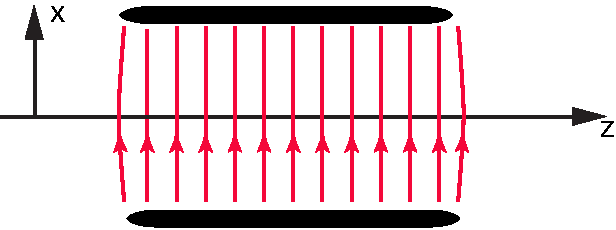
\includegraphics[width=5in]{elseparator.pdf}
  \caption[ElSeparator electric field.]
  {
Elseparator Electric field. The fringe field lines break the
translational invariance in $x$.
  }
  \label{f:elsep}.
\end{figure}

[Thanks to \'Etienne Forest for the derivation of the elseparator equation of motion.]

The Hamiltonian for an electric separator is 
\Begineq
  H = -p_s 
  = - \left\{ \left( \frac{1}{\beta_0} + \delta + k_E \, x \right)^2 - 
  \wt m^2 - p_x^2 - p_y^2 \right\}^{1/2}
  \label{hp1b}
\Endeq
Here the canonical coordinates $(-c \, t, \delta$ are being used,
$\wt m$ is defined in \Eq{mmccp}, and $p_s = -H$ is just the
longitudinal momentum.  In the above equation, $k_E$ is the normalized
field
\Begineq
  k_E = \frac{q \, E}{P_0 \, c}
\Endeq
The field is taken to be pointing along the $x$-axis with positive
$k_E$ accelerating a particle in the positive $x$ direction. To solve
the equations of motion, a ``hard edge'' model is used where $k_E$ is
constant inside the separator and the field ends abrouptly at the
separator edges.

\index{solenoid}
Since, as shown in \fig{f:elsep}, the fringe fields break the
translational invariance in $x$, it is important here that the $x = 0$
plane be centered within the separator plates. With this, the
canonical momentum $\delta$ just outside the separator assumes its
free space form of $\delta = (E - E_0) / E_0)$. This is analogous to
the case of a \vn{solenoid} where, to ensure that the canonical
transverse momenta assume their free space form just outside the
solenoid, the $\Bf z$-axis must be along the centerline of the
solenoid.

The solution of the equations of motion is:
\begin{align}
  x   &= (x_0 - x_c) \, \cosh \left( \frac{k_E \, L}{p_s} \right) + 
         \frac{p_{x0}}{k_E} \, \sinh \left( \frac{k_E \, L}{p_s} \right) + x_c \CRNO
  p_x &= k_E \, (x_0 - x_c) \, \sinh \left( \frac{k_E \, L}{p_s} \right) + 
         {p_{x0}} \, \cosh \left( \frac{k_E \, L}{p_s} \right) \CRNO
  y   &= y_0 + L \, \frac{p_{y0}}{p_s} \label{xxlp} \\
  p_y &= p_{y0} \CRNO
  c \, \delta t &=  \int_0^L -\frac{\partial H}{\partial \delta}
      = (x_0 - x_c) \, \sinh \left( \frac{k_E \, L}{p_s} \right) +
        \frac{p_{x0}}{k_E} \, \left[ \cosh \left( \frac{k_E \, L}{p_s} \right) - 1 \right]
        \nonumber
\end{align}
where the critical position $x_c$ is
\Begineq 
  x_c = -\frac{\wt E}{k_E}
\Endeq
and 
\Begineq
  \wt E \equiv \frac{1}{\beta_0} + \delta = \frac{E}{P_0 \, c}
\Endeq
 
\Eqs{xxlp} predict that for $x < x_c$ and $p_{x0} = 0$ a particle
will, unphysically, accelerate in the negative $x$ direction. In
actuality, a particle in this instance will be reflected backwards by
the longitudinal component of the edge field. Specifically, the
argument of the square root in \Eq{hp1b} must be non-negative and
a particle will only make it through the speparator if
\Begineq
  x_0 > \frac{1}{k_E} \, \left( \sqrt{\wt m^2 + p_{x0}^2 + p_{y0}^2} - \wt E \right)
\Endeq

%---------------------------------------------------------------------------------
%---------------------------------------------------------------------------------
\section{Kicker, Hkicker, and Vkicker, Tracking}
\label{s:kicker.std}
\index{kicker}
\index{hkicker}
\index{vkicker}
\index{elseparator}

The Hamiltonian for a horizontally deflecting kicker or separator is
\Begineq
  H = \frac{p_x^2 + p_y^2}{2 (1 + p_z)} - k_0 \, x 
\Endeq
This gives the map
\begin{align}
  x_2    &= x_1 + \frac{1}{1 + p_{z1}} \, \left( L \, p_{x1} + \frac{1}{2} k_0 \, L^2 \right) \CRNO
  p_{x2} &= p_{x1} + k_0 \, L \CRNO
  y_2    &= y_1 + \frac{L \, p_{y1}}{1 + p_{z1}} \CRNO
  p_{y2} &= p_{y1}  \\
  z_2    &= z_1 - \frac{L}{2 (1 + p_{z1})^2} \, 
    \left( p_{x1}^2 + p_{y1}^2 + p_{x1} \, k_0 \, L + \frac{1}{3} k_0^2 \, L^2 \right) \CRNO
  p_{z2} &= p_{z1} \nonumber
\end{align}
The generalization when the kick is not in the horizontal plane is easily derived.

%---------------------------------------------------------------------------------
%---------------------------------------------------------------------------------
\section{Lcavity Tracking}
\label{s:lcavity.std}
\index{lcavity}

The transverse trajectory through an \vn{Lcavity} is modeled using equations
developed by Rosenzweig and Serafini\cite{b:rosenzweig} (R\&S) with
\begin{align}
  b_0 &= 1 \CRNO
  b_{-1} &= 1 
\end{align}
and all other $b_n$ set to zero.

The transport equations in R\&S were developed in the
ulta-relativistic limit with $\beta = 1$.  To extend these equations,
the transport through the cavity body (R\&S Eq.~(9)) has been modified
to give the correct phase-space area at non ultra-relativistic
energies:
\Begineq
  \begin{pmatrix}
    x \\ 
    x'
  \end{pmatrix}_2 = 
  \begin{pmatrix}
    \cos(\alpha)  &  
    \sqrt{\frac{8}{\eta(\Delta\phi)}} \, \frac{\beta_1 \, \gamma_1}{\gamma'} \, 
                                                   \cos(\Delta\phi) \, \sin(\alpha) \\
    -\sqrt{\frac{\eta(\Delta\phi)}{8}} \, 
                     \frac{\gamma'}{\beta_2 \, \gamma_2 \, \cos(\Delta\phi)} \, \sin(\alpha) &
    \frac{\beta_1 \, \gamma_1}{\beta_2 \, \gamma_2} \, \cos(\alpha)
  \end{pmatrix}
  \,
  \begin{pmatrix}
    x \\ 
    x'
  \end{pmatrix}_1
\Endeq
The added factors of $\beta$ give the matrix the correct determinate
of $\beta_1 \, \gamma_1 / \beta_2 \, \gamma_2$. {\em While the added
factors of $\beta$ do correct the phase space area, the above equation
can only be considered as a rough approximation for simulating
particles when $\beta$ is significantly different from 1. Indeed, the
only accurate way to simulate such particles is by integrating through
the actual field [Cf.~Runge Kutta tracking (\sref{s:tkm})]}

The change in $z$ going through a cavity is calculated by first calculating the particle
transit time $\Delta t$
\begin{align}
  c \, \Delta t &= \int_{s_1}^{s_2} \!\! ds \,\, \frac{1}{\beta(s)} \CRNO
  &= \int_{s_1}^{s_2} \!\! ds \, \frac{E}{\sqrt{E^2 - (mc^2)^2}} \\
  &= \frac{c \, P_{z2} - c \, P_{z1}}{G} \nonumber
\end{align}
where it has been assumed that the accelerating gradient $G$ is
constant through the cavity. In this equation $\beta = v / c$, $E$ is
the energy, and $P_{z1}$ and $P_{z2}$ are the entrance and exit
momenta. Using \Eq{zbctt}, the change in $z$ is thus
\Begineq
  z_2 = \frac{\beta_2}{\beta_1} \, z_1 - 
  \beta_2 \, 
  \left(
  \frac{c \, P_{z2} - c \, P_{z1}}{G} - 
  \frac{c \, \Pbar_{z2} - c \, \Pbar_{z1}}{\BAR G}
  \right)
\Endeq
where $\Pbar$ and $\BAR G$ are the momentum and gradient of the
reference particle.

Note that the above transport equations are only symplectic on-axis
There are second order terms in the transverse coordinates that are
missing. To obtain a proper symplectic matrix, the \vn{symplectify}
attribute of an \vn{lcavity} element (\sref{s:symp}) can be set to
True.

%---------------------------------------------------------------------------------
%---------------------------------------------------------------------------------
\section{Octupole Tracking}
\label{s:octupole.std}
\index{octupole}

The Hamiltonian for an upright octupole is
\Begineq
  H = \frac{p_x^2 + p_y^2}{2 (1 + p_z)} + \frac{k_3}{24} (x^4 - 6 \, x^2 \, y^2 + y^4)
\Endeq

An octupole is modeled using a kick-drift-kick model.

%---------------------------------------------------------------------------------
%---------------------------------------------------------------------------------
\section{Patch Tracking}
\label{s:patch.std}
\index{patch}

\begin{figure}[tb]
  \centering
  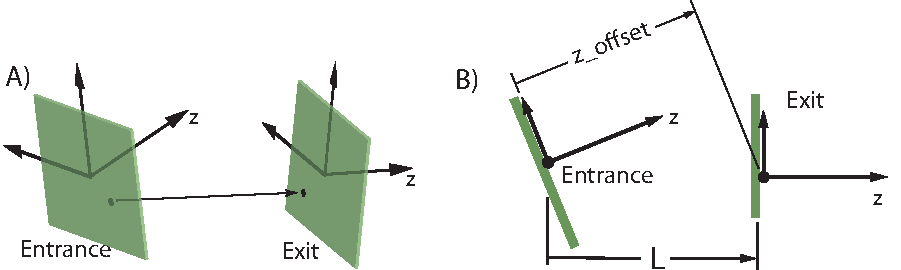
\includegraphics[width=5in]{patch.pdf}
  \caption[Standard patch transformation.]
{Standard tracking through a patch element. A particle's starting coordinate at
the entrance end of the patch has, by construction, coordinate $z$ =
0. The particle is drifted, as in a field free region, between the
entrance $z = 0$ plane and the exit $z = 0$ plane.}
  \label{f:patch.track}
\end{figure}

%---------------------------------------------------------------------------------

The transformation of the reference coordinates through a ``standard''
patch (a patch where custom fields are not used) is given by
\Eqs{vwlv} and \eq{wws}. At the entrance end of the patch, a
particle's position and momentum in the entrance coordinate system will be
\begin{alignat}{1}
  \bfr &= (x, y, 0) \CRNO
  \bfP &= (P_x, P_y, P_z) = 
    \left( p_x, p_y, \pm \sqrt{(1+p_z)^2 - p_x^2 - p_y^2} \right) \, P_{0\text{ent}}
\end{alignat}
where $p_x$, $p_y$ and $p_z$ are the phase space momenta, and $z$,
which is coordinate $z$ and not phase space $z$, is always zero by
construction as shown in \fig{f:patch.track} [Also see \fig{f:local.coords}
and the discussion in \sref{s:phase.space}.] The sign of the
longitudinal momentum $P_z$ is determined by whether the particle is
traveling in the positive $s$ or negative $s$ direction (which will
occur when an element is flipped longitudinally).

The transformation between entrance and exit coordinate systems is given by \Eqs{rwlr} and \eq{pps}
\begin{alignat}{1}
  \bfr &\rightarrow 
    \bfS^{-1} \, (\bfr - \bfL_\text{off}) \CRNO
  \bfP &\rightarrow \bfS^{-1} \, \bfP
\end{alignat}
where $\bfL_\text{off}$ is given by \Eq{swww}

After this transformation, the particle must be propagated by a longitudinal length
$-r_z$ to intersect the $r_z = 0$ plane of the exit face.
\begin{alignat}{1}
  \bfr &\rightarrow (r_x - r_z \, \frac{P_x}{P_z}, r_y - r_z \, \frac{P_y}{P_z}, 0) \CRNO
  \bfP &\rightarrow \bfP
\end{alignat}

The final $\bfr$ and $\bfP$ can now be used compute the particles
phase space coordinates, along with the time $t$ and the reference time
$t_{\text{ref}}$ at the exit end.
\begin{alignat}{3}
  x &\rightarrow r_x \qquad &p_x &\rightarrow \frac{P_x}{P_{0\text{exi}}} \CRNO
  y &\rightarrow r_y \qquad &p_y &\rightarrow \frac{P_y}{P_{0\text{exi}}} \\
  z &\rightarrow z + r_z \, \frac{|\bfP|}{P_z} + L_0 \, \frac{\beta}{\beta_0} +
    \beta \, \text{t_offset} \qquad
    &p_z &\rightarrow \frac{(1+p_z) \, P_{0\text{ent}} - P_{0\text{exi}}}{P_{0\text{exi}}} \CRNO
  t &\rightarrow t - r_z \, \frac{|\bfP|}{P_z \, \beta} \qquad
  &t_{\text{ref}} &\rightarrow t_{\text{ref}} + \text{t_offset} + L_0 \, \frac{1}{\beta_0} \nonumber
\end{alignat}
where the exit reference momentum $P_{0\text{exi}}$ is related to the
entrance reference momentum $P_{0\text{ent}}$ through
\vn{e_tot_offset}.  In the above equation, $\beta$ is the particle
velocity, $\beta_0$ is the velocity of the reference particle, and
$L_0$ is the drift length of the reference particle
\Begineq
  L_0 = \frac{1}{S^{-1}_{33}} \, \left( 
  S^{-1}_{31} \, \text{x_offset} + S^{-1}_{32} \, \text{y_offset} + S^{-1}_{33} \, \text{z_offset}
  \right)
\Endeq

%---------------------------------------------------------------------------------
%---------------------------------------------------------------------------------
\section{Quadrupole Tracking}
\label{s:quadrupole.std}
\index{quadrupole}

The \vn{bmad_standard} calculates the transfer map through an upright
quadrupole and then transforms that map to the laboratory frame.

The Hamiltonian for an upright quadrupole is
\Begineq
  H = \frac{p_x^2 + p_y^2}{2 (1 + p_z)} + \frac{k_1}{2} (x^2 - y^2)
\Endeq
This is simply solved
\begin{align}
  x_2    &= c_x \, x_1 + s_x \, \frac{p_{x1}}{1 + p_{z1}} \CRNO
  p_{x2} &= \tau_x \, \om^2 \, \, (1 + p_{z1}) \, s_x \, x_1 + c_x \, p_{x1} \CRNO
  y_2    &= c_y \, y_1 + s_y \, \frac{p_{y1}}{1 + p_{z1}} \CRNO
  p_{y2} &= \tau_y \, \om^2 \, \, (1 + p_{z1}) \, s_y \, y_1 + c_y \, p_{y1} \\
  z_2    &= z_1 + m_{511} \, x_1^2 + m_{512} \, x_1 \, p_{x1} + m_{522} \, p_{x1}^2 + 
                   m_{533} \, y_1^2 + m_{534} \, y_1 \, p_{y1} + m_{544} \, p_{y1}^2 \CRNO
  p_{z2} &= p_{z1} \nonumber
\end{align}
where 
\Begineq
  \om \equiv \sqrt{\frac{|k_1|}{1 + p_{z1}}}
\Endeq
and
\begin{alignat}{6}
         &\hspace*{3ex}  && k_1 > 0          &\hspace*{3ex}& k_1 < 0 & \qqquad
         &\hspace*{3ex}  && k_1 > 0          &\hspace*{3ex}& k_1 < 0 \CRNO
     c_x &=   && \cos  (\om \, L) && \cosh (\om \, L) & \qqquad
     c_y &=   && \cosh (\om \, L) && \cos  (\om \, L) \CRNO
     s_x &=   && \frac{\sin  (\om \, L)}{\om} && \frac{\sinh (\om \, L)}{\om} & \qqquad
     s_y &=   && \frac{\sinh (\om \, L)}{\om} && \frac{\sin  (\om \, L)}{\om} \\
  \tau_x &=   && {-}1             && {+}1             & \qqquad
  \tau_y &=   && {+}1             && {-}1             \nonumber
\end{alignat}
with this
\begin{alignat}{2}
  m_{511} &= \frac{\tau_x \,\, \om^2}{4} \, (L - c_x \, s_x) & \qqquad
  m_{533} &= \frac{\tau_y \,\, \om^2}{4} \, (L - c_y \, s_y) \CRNO
  m_{512} &= \frac{-\tau_x \,\, \om^2}{2 \, (1 + p_{z1})} \, s_x^2 & \qqquad
  m_{534} &= \frac{-\tau_y \,\, \om^2}{2 \, (1 + p_{z1})} \, s_y^2 \\
  m_{522} &= \frac{-1}{4 \, (1 + p_{z1})^2} \, (L + c_x \, s_x) & \qqquad
  m_{544} &= \frac{-1}{4 \, (1 + p_{z1})^2} \, (L + c_y \, s_y) \nonumber
\end{alignat}

%---------------------------------------------------------------------------------
%---------------------------------------------------------------------------------
\section{RFcavity Tracking}
\label{s:rfcavity.std}
\index{rfcavity}

Tracking through an rfcavity uses a kick-drift-kick model. The kick is
a pure energy kick (see equations in \sref{s:rfcav}) and the phase of
the RF is calculated under the assumption that the waveform moves at a
phase velocity equal to the velocity of the reference particle.

\index{lcavity}
The transverse forces due to the RF are ignored. This is a resonable
approximation when the acceleration is small. \vn{Lcavity} elements
should be used in place of \vn{rfcavity} elements when this is not so.

%---------------------------------------------------------------------------------
%---------------------------------------------------------------------------------
\section{Sad\_Mult Tracking}
\label{s:sad.mult.std}
\index{sad_mult}

The ``hard edge'' fringe field kick is taken from Forest\cite{b:forest} Eqs.~(13.29) and onward.
In the notation of \bmad, and taking into account both normal and skew terms, Eq.~(13.29)
is for the $m$\th order multipole (what Forest labels $n+1$)
\Begineq
  f_\pm = \mp \Re \frac{(b_m + i \, a_m) \, (x + i \, y)^{(m+1)}}{4 \, (m+2) \, (1 + p_z)}
    \left[ x \, p_x + y \, p_y + i\frac{m+3}{m+1}(x \, p_y - y \, p_x) \right]
\Endeq

The ``soft edge'' dipole fringe for \vn{sad_mult} elements is a generalization of the soft edge
dipole fringe for a SAD bend element. For the entrance kick the equations are:
\begin{align}
  x_2 &= x_1 + \frac{\delta_1}{1 + \delta_1} \, \Delta x_{fx}, \qquad
  p_{x2} = p_{x1} + \frac{1}{1 + \delta_1} \, \left[ 
    \Delta x_{fy} \, v - \Delta x_{fay} \, v^3 \right] \CRNO
  y_2 &= y_1 - \frac{\delta_1}{1 + \delta_1} \, \Delta y_{fy}, \qquad
  p_{y2} = p_{y1} + \frac{1}{1 + \delta_1} \, \left[ 
    \Delta y_{fx} \, w - \Delta y_{fax} \, w^3 \right] \\
  z_2 &= z_1 + \frac{1}{(1 + \delta_1)^2} \, \left[ \, 
    \Delta x_{fx} \, p_{x1} - \Delta y_{fy} \, p_{y1} + 
    \frac{1}{2} \, (\Delta y_{fx} + \Delta x_{fy}) \, w^2 -
    \frac{1}{4} (\Delta y_{fax} + \Delta x_{fay}) \, w^4
    \right] \nonumber
\end{align}
where
\begin{alignat}{3}
  \Delta x_{fx}  &= \frac{K_0 \, F_B^2}{24 \, L}, & \qquad 
  \Delta y_{fx}  &= \frac{K_0^2 \, F_B}{6 \, L^2}, & \qquad 
  \Delta y_{fax} &= \frac{2 \, K_0^2}{3 \, F_B \, L^2}, \CRNO 
  \Delta y_{fy}  &= \frac{SK_0 \, F_B^2}{24 \, L}, & \qquad
  \Delta x_{fy}  &= \frac{SK_0^2 \, F_B}{6 \, L^2}, & \qquad
  \Delta x_{fay} &= \frac{2 \, SK_0^2}{3 \, F_B \, L^2}, \\
  v &= \cos\theta \, x_1 + \sin\theta \, y_1, & \qquad
  w &= -\sin\theta \, x_1 + \cos\theta \, y_1, & \qquad
  \tan\theta &= \frac{-SK_0}{K_0} \nonumber
\end{alignat}


%---------------------------------------------------------------------------------
%---------------------------------------------------------------------------------
\section{Sextupole Tracking}
\label{s:sextupole.std}
\index{sextupole}

The Hamiltonian for an upright sextupole is
\Begineq
  H = \frac{p_x^2 + p_y^2}{2 (1 + p_z)} + \frac{k_2}{6} (x^3 - 3 \, x \, y^2)
\Endeq

Tracking through a sextupole uses a kick-drift-kick model.

%---------------------------------------------------------------------------------
%---------------------------------------------------------------------------------
\section{Sol\_Quad Tracking}
\label{s:sol.quad.std}
\index{sol_quad}

The Hamiltonian is
\Begineq
  H = \frac{(p_x + \frac{k_s }{2}\, y)^2}{2 (1 + p_z)} + 
  \frac{(p_y - \frac{k_s}{2} \, x)^2}{2 (1 + p_z)} + \frac{k_1}{2} (x^2 - y^2)
\Endeq
Solving the equations of motion gives
\begin{align}
  x_2    &= m_{11} \, x_1 + m_{12} \, p_{x1} + m_{13} \, y_1 + m_{14} \, p_{y1} \CRNO
  p_{x2} &= m_{21} \, x_1 + m_{22} \, p_{x1} + m_{23} \, y_1 + m_{24} \, p_{y1} \CRNO
  y_2    &= m_{31} \, x_1 + m_{32} \, p_{x1} + m_{33} \, y_1 + m_{34} \, p_{y1} \CRNO
  p_{y2} &= m_{41} \, x_1 + m_{42} \, p_{x1} + m_{43} \, y_1 + m_{44} \, p_{y1} \\
  z_2    &= z_1 + \sum_{j = 1}^4 \sum_{k = j}^4 m_{5jk} \, r_j \, r_k  \CRNO
  p_{z2} &= p_{z1} \nonumber
\end{align}
where
\begin{alignat}{2}
  m_{11} &= \frac{1}{2 \, f} \, \left( f_{0+} \, c + f_{0-} \, c_h \right) & \qqquad
  m_{31} &= -m_{24} \CRNO
  m_{12} &= \frac{1}{2 \, f \, (1 + p_{z1})} \, 
            \left( \frac{f_{++}}{\om_+} \,  s + \frac{f_{--}}{\om_-} \, s_h \right) & \qqquad
  m_{32} &= -m_{14} \CRNO
  m_{13} &= \frac{\ks}{4 \, f} \, 
            \left( \frac{f_{+-}}{\om_+} \, s +\frac{f_{-+}}{\om_-} \, s_h \right) & \qqquad
  m_{33} &= \frac{1}{2 \, f} \, \left( f_{0-} \, c + f_{0+} \, c_h \right) \CRNO
  m_{14} &= \frac{\ks}{f \, (1 + p_{z1})} \, \left( -c + c_h \right) & \qqquad
  m_{34} &= \frac{1}{2 \, f \, (1 + p_{z1})} \, 
            \left( \frac{f_{+-}}{\om_+} \, s + \frac{f_{-+}}{\om_-} \, s_h \right) \CRNO
  m_{21} &= \frac{-(1 + p_{z1})}{8 \, f} \, 
            \left( \frac{\xi_{1+}}{\om_+} \, s + \frac{\xi_{2+}}{\om_-} s_h \right) & \qqquad
  m_{41} &= -m_{23} \\
  m_{22} &= m_{11} & \qqquad
  m_{42} &= -m_{13} \CRNO
  m_{23} &= \frac{\ks^3 \, (1 + p_{z1})}{4 \, f} \, \left( c - c_h \right) & \qqquad
  m_{43} &= \frac{-(1 + p_{z1})}{8 \, f} \, 
            \left( \frac{\xi_{1-}}{\om_+} \, s + \frac{\xi_{2-}}{\om_-} \, s_h \right) \CRNO
  m_{24} &= \frac{\ks}{4 \, f} \, 
            \left( \frac{f_{++}}{\om_+} \, s + \frac{f_{--}}{\om_-} \, s_h \right) & \qqquad
  m_{44} &= m_{33} \nonumber
\end{alignat}
and
\begin{alignat}{2}
  \kone        &= \frac{k_1}{1 + p_{z1}} & \qqquad 
  \ks          &= \frac{k_s}{1 + p_{z1}} \CRNO
  f            &= \sqrt{\ks^4 + 4 \, \kone^2} & \qqquad
  f_{\pm0}     &= f \pm \ks^2 \CRNO
  f_{0\pm}     &= f \pm 2 \, \kone & \qqquad
  f_{\pm\pm}   &= f \pm \ks^2 \pm 2 \, \kone \CRNO
  \om_+        &= \sqrt{\frac{f_{+0}}{2}} & \qqquad
  \om_-        &= \sqrt{\frac{f_{-0}}{2}} \\
  s            &= \sin (\om_+ \, L) & \qqquad
  s_h          &= \sinh (\om_- \, L) \CRNO
  c            &= \cos (\om_+ \, L) & \qqquad
  c_h          &= \cosh (\om_- \, L) \CRNO
  \xi_{1\pm} &= \ks^2 \, f_{+\mp} \pm 4 \, \kone \, f_{+\pm} & \qqquad
  \xi_{2\pm} &= \ks^2 \, f_{-\pm} \pm 4 \, \kone \, f_{-\mp} \nonumber
\end{alignat}

The $m_{5jk}$ terms are obtained via \Eq{zz121p}
\begin{align}
  m_{5jk} = - \frac{\tau_{jk}}{2 (1 + p_{z1})^2} \int \! ds \, 
  & \left[ 
    \left( m_{2j} + \frac{k_s}{2} \, m_{3j} \right) \, 
    \left( m_{2k} + \frac{k_s}{2} \, m_{3k} \right)   
  \right. + \\
  & \hspace*{15ex} \left.
    \left( m_{4j} - \frac{k_s}{2} \, m_{1j} \right) \, 
    \left( m_{4k} - \frac{k_s}{2} \, m_{1k} \right) 
  \right] \nonumber
\end{align}
where
\Begineq
  \tau_{jk} = 
  \begin{cases}
    1 & j = k \\
    2 & j \ne k 
  \end{cases}
\Endeq
The needed integrals involve the product of two trigonometric or
hyperbolic functions. These integrals are trivial to do but the
explicit equations for $m_{5jk}$ are quite long and in the interests of
brevity are not reproduced here.

%---------------------------------------------------------------------------------

\begin{figure}[tb]
  \centering
  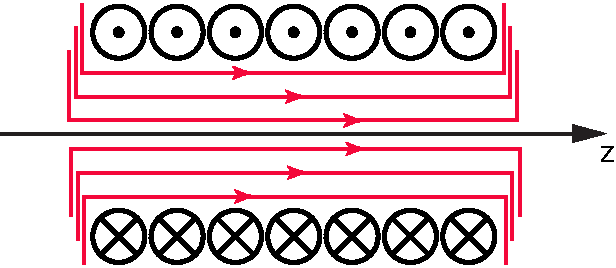
\includegraphics[width=5in]{solenoid.pdf}
  \caption[Solenoid with a hard edge.]
  {
Solenoid with a hard edge. The field is assumed to end abruptly at the
edges of the solenoid. Here, for purposes of illustration, the field lines at
the ends are displaced from one another.
  }
  \label{f:solenoid}.
\end{figure}

%---------------------------------------------------------------------------------
%---------------------------------------------------------------------------------
\section{Solenoid Tracking}
\label{s:solenoid.std}
\index{solenoid}

The Hamiltonian for a solenoid is
\Begineq
  H = \frac{ \left( p_x + \frac{k_s}{2} \, y \right)^2}{2 \, (1 + p_z)} + 
  \frac{ \left( p_y - \frac{k_s}{2} \, x \right)^2}{2 \, (1 + p_z)} 
\Endeq
where the normalized field $k_s$ is
\Begineq
  k_s = \frac{B}{P_0}
\Endeq
The solution to the equations of motion for a constant $k_s$ are
\begin{align}
  x_2    &= \frac{1 + c}{2} \, x_1 + \frac{s}{k_s} \, p_{x1} +
           \frac{s}{2} \, y_1 + \frac{1 - c}{k_s} \, p_{y1} \CRNO
  p_{x2} &= \frac{-k_s \, s}{4} \, x_1 + \frac{1 + c}{2} \, p_{x1} - 
           \frac{k_s \, (1 - c)}{4} \, y_1 + \frac{s}{2} \, p_{y1} \CRNO
  y_2    &= \frac{-s}{2} \, x_1 - \frac{1 - c}{k_s} \, p_{x1} +
           \frac{1 + c}{2} \, y_1 + \frac{s}{k_s} \, p_{y1} \\      
  p_{y2} &= \frac{k_s \, (1 - c)}{4} \, x_1 + \frac{-s}{2} \, p_{x1} -
            \frac{k_s \, s}{4} \, y_1 + \frac{1 + c}{2} \, p_{y1} \CRNO 
  z_2    &= z_1 + \frac{L}{2 \, (1 + p_{z1})^2} \, 
                   \left[ \left( p_{x1} + \frac{k_s}{2} \, y_1 \right)^2 +
                          \left( p_{y1} - \frac{k_s}{2} \, x_1 \right)^2 \right] \CRNO
  p_{z2} &= p_{z1} \nonumber
\end{align}
where
\begin{align}
  c &= \cos \left( \frac{k_s}{2} \, L \right) \CRNO
  s &= \sin \left( \frac{k_s}{2} \, L \right)
\end{align}

To be useful, the canonical momenta $p_x$ and $p_y$ in the above
equations must be connected to the cononical momenta used for other
elements (drifts, quadrupoles, etc.) that may be placed to either side
of the solenoid. These side elements use zero $a_x$ and $a_y$
(cf. \Eq{pmc2pc}). The vector potential used in the solenoid canonical
momenta may be made zero at the edges of the solenoid if the solenoid
fringe field is assumed to end abruptly at the edges of the solenoid
(as shown in \fig{f:solenoid}), and the reference axis $\Bf z$-axis (at
$x$ = $y$ = 0) is placed along the centerline of the solenoid so that
there is cylendrical symmetry around the $\Bf z$-axis.

%---------------------------------------------------------------------------------
\section{Symplectic Tracking with Cartesian Modes}
\label{s:wiggler.std}
\index{wiggler!tracking}

The method for symplectic integration for elements that define the magnetic field using a
Cartesian mode decomposition (\sref{s:cart.map}) is outlined in \sref{s:symp.track}.  The
vector potential is constructed to avoid singularities when one of the wave vectors $k_x$,
$k_y$, or $k_z$ is zero.

For the \vn{x} \vn{family} the vector potential is:
\begin{center}
{
\setlength{\tabcolsep}{1pt}
\begin{tabular}{lrllrllrll}
  Form \; & \multicolumn{3}{l}{hyper-y}  & \multicolumn{3}{l}{hyper-xy}  & \multicolumn{3}{l}{hyper-x} \\
  $A_x$   & 
    $A$ & $\dfrac{k_z}{k_y^2}$      & $\Se_x \, \Sh_y \, \Se_z \qquad$ &
    $A$ & $\dfrac{1}{k_y}$          & $\Sh_x \, \Sh_y \, \Se_z \qquad$ &
    $A$ & $\dfrac{k_z}{k_x \, k_y}$ & $\Sh_x \, \Se_y \, \Se_z$ \\
  $A_y$   & 0 &&& 0 &&& 0 && \\
  $A_z$   & 
    $A$ & $\dfrac{k_x}{k_y^2}$      & $\Ce_x \, \Sh_y \, \Ce_z \qquad$ &
    $A$ & $\dfrac{k_x}{k_y \, k_z}$ & $\Ch_x \, \Sh_y \, \Ce_z \qquad$ &
    $A$ & $\dfrac{1}{k_y}$          & $\Ch_x \, \Se_y \, \Ce_z$ 
\end{tabular}
}
\end{center}

For the \vn{y} \vn{family} the vector potential is:
\begin{center}
{
\setlength{\tabcolsep}{1pt}
\begin{tabular}{lrllrllrll}
  Form \; & \multicolumn{3}{l}{hyper-y}  & \multicolumn{3}{l}{hyper-xy}  & \multicolumn{3}{l}{hyper-x} \\
  $A_x$   & 0 &&& 0 &&& 0 && \\
  $A_y$   & 
    $-A$ & $\dfrac{k_z}{k_x \, k_y}$ & $\Se_x \, \Sh_y \, \Se_z \qquad$ &
    $-A$ & $\dfrac{1}{k_x}$          & $\Sh_x \, \Sh_y \, \Se_z \qquad$ &
    $-A$ & $\dfrac{k_z}{k_x^2}$      & $\Sh_x \, \Se_y \, \Se_z$ \\
  $A_z$   & 
    $-A$ & $\dfrac{1}{k_x}$          & $\Se_x \, \Ch_y \, \Ce_z \qquad$ &
    $-A$ & $\dfrac{k_y}{k_x \, k_z}$ & $\Sh_x \, \Ch_y \, \Ce_z \qquad$ &
    $-A$ & $\dfrac{k_y}{k_x^2}$      & $\Sh_x \, \Ce_y \, \Ce_z$ 
\end{tabular}
}
\end{center}

For the \vn{qu} \vn{family} the vector potential is:
\begin{center}
{
\setlength{\tabcolsep}{1pt}
\begin{tabular}{lrllrllrll}
  Form \; & \multicolumn{3}{l}{hyper-y}  & \multicolumn{3}{l}{hyper-xy}  & \multicolumn{3}{l}{hyper-x} \\
  $A_x$   & 
     $A$ & $\dfrac{1}{k_z}$          & $\Se_x \, \Ch_y \, \Se_z \qquad$ &
     $A$ & $\dfrac{k_y}{k_z^2}$      & $\Sh_x \, \Ch_y \, \Se_z \qquad$ &
     $A$ & $\dfrac{k_y}{k_x \, k_z}$ & $\Sh_x \, \Ce_y \, \Se_z$ \\
  $A_y$   & 
    $-A$ & $\dfrac{k_x}{k_y \, k_z}$ & $\Ce_x \, \Sh_y \, \Se_z \qquad$ &
    $-A$ & $\dfrac{k_x}{k_z^2}$      & $\Ch_x \, \Sh_y \, \Se_z \qquad$ &
    $-A$ & $\dfrac{1}{k_z}$          & $\Ch_x \, \Se_y \, \Se_z$ \\
  $A_z$   & 0 &&& 0 &&& 0 &&
\end{tabular}
}
\end{center}

For the \vn{sq} \vn{family} the vector potential is:
\begin{center}
{
\setlength{\tabcolsep}{1pt}
\begin{tabular}{lrllrllrll}
  Form \; & \multicolumn{3}{l}{hyper-y}  & \multicolumn{3}{l}{hyper-xy}  & \multicolumn{3}{l}{hyper-x} \\
  $A_x$   & 
     $A$ & $\dfrac{1}{k_z}$          & $\Ce_x \, \Sh_y \, \Se_z \qquad$ &
     $A$ & $\dfrac{k_y}{k_z^2}$      & $\Ch_x \, \Sh_y \, \Se_z \qquad$ &
     $A$ & $\dfrac{k_y}{k_x \, k_z}$ & $\Ch_x \, \Se_y \, \Se_z$ \\
  $A_y$   & 
     $A$ & $\dfrac{k_x}{k_y \, k_z}$ & $\Se_x \, \Ch_y \, \Se_z \qquad$ &
    $-A$ & $\dfrac{k_x}{k_z^2}$      & $\Sh_x \, \Ch_y \, \Se_z \qquad$ &
     $A$ & $\dfrac{1}{k_z}$          & $\Sh_x \, \Ce_y \, \Se_z$ \\
  $A_z$   & 0 &&& 0 &&& 0 &&
\end{tabular}
}
\end{center}


\chapter{Tracking of X-Rays}
\label{c:xray.track}

\bmad can track both charged particles and X-rays. This chapter deals
with X-rays. Charged particles are handled in chapter~\sref{c:charged.track}.

%-------------------------------------------------------------------------
%-------------------------------------------------------------------------
\section{Coherent and Incoherent Photon Simulations}
\label{s:coher.incoher}

\index{coherent tracking}\index{incoherent tracking}
\bmad can track photons either \vn{coherenly} or \vn{incoherently}.
In both cases, the photon has a transverse electric field 
\Begineq
  (E_x, E_y)
\Endeq
$E_x$ and $E_y$ are complex and therefore have both amplitude and phase
information. When photons are tracked incoherently, the phase
information is not used for calculating X-ray intensities.

In addition to coherent and incoherent tracking, partially coherent
simulations can be done by using sets of photons with the photons in
any one set treated as coherent and the photons between sets being
treated as incoherent.

%-------------------------------------------------------------------------
\subsection{Incoherent Photon Tracking}
\label{s:incoher}

In a simulation with incoherent photons, some number of photons,
$N_0$, will be generated and the i\Th photon ($i = 1, \ldots, N_0)$
will have a initial ``electric field'' components $E_{x0}(i),
E_{y0}(i)$ assigned to it. The field amplitude $E_0$ will be
$\sqrt{E_{x0}^2 + E_{y0}^2}$.

At some an observation point, the power $S$ per unit area falling on
some small area $dA$ due to either $x$ or $y$ component of the
electric field is
\Begineq
  S_{x,y} = \frac{\alpha_p}{N_0 \, dA} \, \sum_{j \in \text{hits}} E_{x,y}^2(j)
  \label{panda1}
\Endeq
where $\alpha_p$ is a constant that can be chosen to fit the
simulation against experimental results, and the sum is over photons
who intersect the area. The factors of $N_0$ and $dA$ in the above
equation make, within statistical flucuations, $S$ independent of
$N_0$ and, for $dA$ small enough, $S$ will be independent of $dA$ as
it should be. The total power is just $S_x + S_y$.

When traveling through vacuum, the electric field of a photon is a
constant.  As an example, consider a point source raidiating uniformly
in $4\pi$ solid angle with each photon having the same initial field
$E_0$. An observation area $dA$ situated a distance $R$ from the
source will intercept $N_0 \, dA / 4 \, \pi \, R^2$ photons which
gives a power of
\Begineq
  S_w = \frac{\alpha_p \, E_0^2}{4 \, \pi \, R^2}
\Endeq
which falls off as $1/R^2$ as expected.

At some places the light may be split into various ``channels''. An
example is Laue diffraction where X-rays can excite the $\alpha$ and
$\beta$ branches of the dispersion surface. Or a partially silvered
mirror where some of the light is reflected and some is transmitted.
In such a case, the probability $P_i$ of a photon traveling down the
$i$\Th channel is
\Begineq
  P_i \, \what E_i^2 = \frac{S_i}{S_0}
  \label{rpss1}
\Endeq
where $S_i$ is the power flowing into channel $i$, $S_0$ is the power
flowing into the junction, and $\what E_i = E_i / E_0$ is the ratio of
the electric field amplitudes of any photon just before and just after being
shunted into the $i$\Th channel. The probabilities must be properly
normalized
\Begineq
  \sum P_i = 1
  \label{p1}
\Endeq

If the ratio of the electric field of any photon just before and just
after being shunted into the $i$\Th channel is not a constant, than
$\what E_i$ must be adjusted so that $\what E_i^2$ is equal to the average of
$\what E_i^2(j)$ for all photons $j$ channeled into channel $i$.

As long as \Eqs{rpss1} and \eq{p1} are satisfied, the choice of the
$P_i$, and $\what E_i$ are arbitrary. This freedom allows simulation to be
optimized for efficiency. For example, In an actual experiment much of
the light can be lost never to reach a detector and be counted. To
decrease the simulation time, simulated photons may be limited to be
generated with a direction to be within some solid angle $\Omega_1$ if
photons with a direction outside this solid angle will not contribute
to the simulation results. In this case, there are two channels.
Channel 1 consists of all photons whose direction is within
$\Omega_1$ and channel 2 is all the other photons. To limit the
photons to channel 1, $P_1$ is taken to be 1 and $P_2$ is taken to be
0. Additionaly, if the light, say, is being generated isotropically
from a surface into a $\Omega_0 = 2 \, \pi$ solid angle then
\Begineq
  \what E_1 = \sqrt{\frac{\Omega_1}{\Omega_0}}
  \label{roo}
\Endeq
$\what E_2$ is infinite here but since no photons are generated in channel 2
this is not a problem.

%-------------------------------------------------------------------------
\subsection{Coherent Photon Tracking}
\index{ss:coher}

In a simulation with coherent photons, some number of photons,
$N_0$, will be generated and the i\Th photon ($i = 1, \ldots, N_0)$
will have an initial electric field $E_{x0}(i), E_{y0}(i)$ assigned to
it. These quantities will be complex.

At some an observation point, the field $E$ at
some small area $dA$ due to either $x$ or $y$ component of the
electric field is
\Begineq
  E = \frac{\alpha_p}{N_0 \, dA} \, \sum_{j \in \text{hits}} E(j)
  \label{panda2}
\Endeq
where $\alpha_p$ is a constant that can be chosen to fit the
simulation against experimental results, and the sum is over photons
who intersect the area. In the above equation $E(j)$ is either the $x$
or $y$ component of the electric field as is appropriate. The factors
of $N_0$ and $dA$ in the above equation make, within statistical
flucuations, $E$ independent of $N_0$ and, for $dA$ small enough, $E$
will be independent of $dA$ as it should be.

When traveling through a a vacuum, the photons travel ballistically in
straight lines. This is justified by using the stationary phase
approximation with Kirchhoff's integral. the electric field of a
photon varies with the propagation length. There is nothing physical
in this and is just a way to make the bookkeeping come out
correctly. As an example, consider a point source raidiating uniformly
in $4\pi$ solid angle with each photon having the same initial field
component (either $x$ or $y$) $E_1$.  An observation area $dA$
situated a distance $R$ from the source will intercept $N_0 \, dA / 4
\, \pi \, R^2$ photons and each photon will have a field of $E_1 \, R
\, \exp(i \, k \, R)$ where $k$ is the photon wave number (all photons
must have the same $k$ to be coherent). This gives an electric field
at the observation point of
\Begineq
  E = \frac{\alpha_p \, E_1 \, \exp(i \, k \, R)}{4 \, \pi \, R}
\Endeq
which falls off as $1/R$ as expected.

At a \vn{diffraction_plate} element where diffraction effects are to
be simulated, the following procedure is used:
  \begin{enumerate}
  \item
The electric field components are multiplied by the propagation length $L$:
\Begineq
  E \rightarrow E \, L
\Endeq
The propagation length is reset to zero so that the at the next point
where the propagation length is factored into the electric field the
propagation length will be the length starting at the aperture.
  \item
Depending upon the program, the photon is is either given a random
direction over $2 \, \pi$ solid angle or the photon's direction
is restricted to be within some solid angle choosen to increase
the probability that the photon will make it through some downstream aperture.

If the photon is restricted to some aperture dependent solid angle of area $\Omega$,
the photon's electric field is scalled by
\Begineq
  E \rightarrow E \, \frac{\Omega}{4 \, \pi}
  \label{eeo4p}
\Endeq

  \item
The electric field components are scaled by
\Begineq
  E \rightarrow E \, \frac{k}{4 \, \pi \, i} \, (\cos\theta_1 + \cos\theta_2)
  \label{eek4p}
\Endeq
where $\theta_1$ and $\theta_2$ are the dirction cosines of the
incoming and outgoing directions of the photon with respect to the
longitudinal reference axis.
  \end{enumerate}
This algorithm is designed so that the resulting fields at points
downstream from the aperture as computed from a simulation will, to
within statistical errors, be the same as one would get using
Kirchoff's integral. That is, the simulation is constructed to be a
Monte Carlo integration of Kirchhoff's integral.

What is, and what is not considered a place where there are
diffraction effects is dependent upon the problem. For example, there
are diffraction effects associated with light reflecting from a mirror
(or any other object) of finite size. If these effects are important
to the experiment, then a procedure similar to the one above must be
followed. 

At places where there are no diffraction effects a simulation can
treat the photons ballistically or can use the aperture procedure
outlined above. While in theory it is possible to choose what to do, in
practice the aperture procedure increases the number of photons that
must be tracked for a given resolution. Thus, from a practical standpoint
the ballistic alternative should always be used.

As explaned in \sref{s:incoher}, at some places the light may be split
into various ``channels''. With coherent photons, the analog to \Eq{rpss1} is
\Begineq
  P_i \, \what E_i = \frac{E_i}{E_0}
  \label{rpss2}
\Endeq
where here $\what E_i$ can be complex to take into account phase shifts.
The same considerations about choosing the $P_i$ and $\what E_i$ apply to
coherent photons as incoherent photons. In particular, $\what E_1$ for the
case of isotropic emission from a surface as in the equample in
\sref{s:incoher} (cf. \Eq{roo}) is
\Begineq
  \what E_1 = \frac{\Omega_1}{\Omega_0}
\Endeq

%-------------------------------------------------------------------------
\subsection{Parially Coherent Photon Simulations}

When there is partial coherence the photons must be divided into
sets. All of the photons of a given set are considered coherent while
the photons of different sets are treated incoherently.

The procedure is to track all the photons of one set coherently and
calculate the field using equation \Eq{panda2}. The fields of
different sets are then combined to calculate a power using
\Eq{panda1}.

%-------------------------------------------------------------------------
%-------------------------------------------------------------------------
\section{Element Coordinate System}
\label{s:photon.ele.coords}

\index{element coordinates}
The general procedure for tracking through an element makes use of
\vn{element reference} coordinates (also called just \vn{element}
coordinates). Without any offsets, pitches or tilt (\sref{s:offset}), henceforth
called ``misalignments'', the \vn{element} coordinates are the same
as the \vn{laboratory reference} coordinates (or simply \vn{laboratory}
coordinates) (\sref{s:ref}). The \vn{element} coordinates stay fixed
relative to the element. Therefore, if the element is misaligned, the
\vn{element coordinates} will follow as the element shifts in the
laboratory frame as shown in \fig{f:ele.coord}.

\index{crystal}\index{mirror}\index{multilayer_mirror}
For \vn{crystal} (\sref{s:crystal}), \vn{mirror} (\sref{s:mirror}),
and \vn{multilayer_mirror} (\sref{s:multilayer}) elements, the
``kinked'' reference trajectory through the element complicates the
calculation. For these elements, there are three coordinate systems
attached to the element as shown in \fig{f:photon.ele.coords}. Besides
the \vn{element entrance} and \vn{element exit} coordinates, there are
\vn{element surface} coordinates with $z$ perpendicular to the surface
pointing inward.

Tracking a particle through an element is therefore a three
step transformation:
\begin{enumerate}
\item
At the entrance end of the element, transform from the laboratory
reference coordinates to the element's \vn{entrance} or \vn{surface}
coordinates.
\item
Track through the element ignoring any misalignments.
\item
At the exit end of the element, transform from the element coordinates
to the \vn{laboratory} \vn{exit} coordinates.
\end{enumerate}


%-------------------------------------------------------------------------

\begin{figure}[tb]
  \centering
  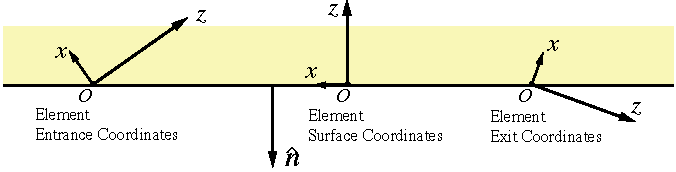
\includegraphics[width=5in]{photon-ele-coords.pdf}
  \caption[Crystal, Mirror, and Multilayer_Mirror Element Coordinates.]
{The three element coordinate systems for \vn{crystal} (Bragg
configuration), \vn{mirror}, and \vn{multilayer_mirror} elements.  The
origin $\Bf O$ of all three are the same but are shown spread out for
clarity.  $\bfhat n$ is the normal to the element surface.}
  \label{f:photon.ele.coords}.
\end{figure}

%-------------------------------------------------------------------------
\subsection{Transform from Laboratory Entrance to Element Coordinates}

For elements that have a reference orbit kink
(\sref{s:photon.ele.coords}), the element coordinates here are the
\vn{surface} coordinates. Otherwise the element coordinates are
the entrance coordinates.

  \begin{enumerate}
  \item
Apply offsets, pitches and tilt using the formulas in
\sref{s:pos.trans} along with \Eqs{wws}, and \eq{swww}.
  \item
Apply the \vn{tilt} to the electric field (\Eq{ertee}).
  \item
For \vn{crystal}, \vn{mirror}, and \vn{multilayer_mirror} elements
rotate to element surface coordinates.
 \item
Transform the photon's position as if in a drift by a distance $-z$
where $z$ is the photon's longitudinal coordinate. That is, $z$ will
be zero at the end of the transform to element coordinates (remember
that $z$ is the distance from the start of the element
(\sref{s:photon.phase.space})).

\end{enumerate}

%-------------------------------------------------------------------------
\subsection{Transform from Element Exit to Laboratory Coordinate}

The back transformation from element to laboratory coordinates is
accomplished by the transformation
  \begin{enumerate}
  \item
For \vn{crystal}, \vn{mirror}, and \vn{multilayer_mirror} elements
rotate to element from element surface coordinates to element exit coordinates
  \item
Apply the reverse \vn{tilt} to the electric field (\Eq{ertee}).
  \item
Apply reverse offsets, pitches and tilt using the formulas in
\sref{s:pos.trans} along with \Eqs{wws}, and \eq{swww}.
  \end{enumerate}

%-------------------------------------------------------------------------
%-------------------------------------------------------------------------
\section[Mirror and Crystal Element Transformation]
{Transformation for Mirror and Crystal Elements Between 
Laboratory and Element Coordinates}
\label{s:photon.lab.ele}

\index{mirror}\index{crystal}

%-------------------------------------------------------------------------
\subsection{Transformation from Laboratory to Element Coordinates}
\label{s:crystal.trans.le}

\index{z_offset_tot}
With photons, the intensities must also be transformed.
The transformation from the the entrance laboratory coordinates to
the entrance element coordinates is:
\begin{enumerate}
\item
Track as in a drift a distance \vn{z_offset_tot}.
\item
\index{x_offset}\index{x_pitch}\index{y_offset}\index{y_pitch}
Apply offsets and pitches: The effective ``length'' of the element is
zero (\sref{s:mirror.coords}) so the origin of the element coordinates
is the same point around which the element is pitched so
\begin{align}
  x_1    &= x_0 - x_{\text{off}} \CRNO
  p_{x1} &= p_{x0} - (1 + p_{z0}) \, x'_{pitch} \CRNO
  y_1    &= y_0 - y_{\text{off}} \\
  p_{y1} &= p_{x0} - (1 + p_{z0}) \, y'_{pitch} \CRNO
  z_1    &= z_0 + x'_{pitch} \, x_1 + y'_{pitch} \, y_1 \nonumber
\end{align}
where $x_{\text{off}} \equiv \vn{x_offset}$, $x'_{pitch} \equiv \vn{x_pitch}$, etc.
\item
Apply \vn{ref_tilt} and \vn{tilt}:
\begin{align}
  \begin{pmatrix} x_2 \\ y_2 \end{pmatrix} &=
    \bfR (\theta_{tot}) \,   
  \begin{pmatrix} x_1 \\ y_1 \end{pmatrix} \CRNO
  \begin{pmatrix} p_{x2} \\ p_{y2} \end{pmatrix} &=
    \bfR (\theta_{tot}) \, 
  \begin{pmatrix} p_{x1} \\ p_{y1} \end{pmatrix} \label{xyrtxy} \\ 
  \begin{pmatrix} \bfE_{x2} \\ \bfE_{y2} \end{pmatrix} &=
    \bfR (\theta_{tot}) \,   \begin{pmatrix} \bfE_{x1} \\ \bfE_{y1} \end{pmatrix} \nonumber
\end{align}
where $\bfE$ is shorthand notation for
\Begineq
  \bfE \equiv E \, e^{i \, \phi}
\Endeq
with $E$ being the field intensity and $\phi$ being the field phase angle.
In the above equations $\bfR$ is the rotation matrix
\Begineq
  \bfR(\theta) = \begin{pmatrix} \cos\theta & \sin\theta \\ -\sin\theta & \cos\theta \end{pmatrix}
\Endeq
\index{tilt}\index{ref_tilt}\index{tilt_corr}
with $\theta_{tot}$ being 
\Begineq
  \theta_{tot}  = 
  \begin{cases}
    \vn{ref_tilt} + \vn{tilt} + \vn{tilt_corr} & \vn{for crystal elements} \\
    \vn{ref_tilt} + \vn{tilt} & \vn{for mirror elements}
  \end{cases}
  \label{tttt}
\Endeq
The \vn{tilt_corr} correction is explained in \sref{s:crystal.trans}.
\end{enumerate}

%-------------------------------------------------------------------------
\subsection{Transformation from Element to Laboratory Coordinates}
\label{s:crystal.trans.el}

The back transformation from exit element coordinates to exit
laboratory coordinates is accomplished by the transformation
  \begin{enumerate}
  \item
Apply \vn{ref_tilt} and \vn{tilt}: \vn{ref_tilt} rotates the exit
laboratory coordinates with respect to the exit element coordinates in
the same way \vn{ref_tilt} rotates the entrance laboratory coordinates
with respect to the entrance element coordinates. The forward and back
transformations are thus just inverses of each other.  With
\vn{tilt}, this is not true. \vn{tilt}, unlike \vn{ref_tilt}, does
not rotate the output laboratory coordinates.  There is the further
complication in that \vn{tilt} is a rotation about the {\em
entrance} laboratory coordinates. The first step is to express
\vn{tilt} with respect to the exit coordinates. This is done with
the help of the $\bfS$ matrix of \Eq{ustt} with $\alpha_t$ given by
\Eq{agg}. The effect of the \vn{tilt} can be modeled as a rotation
vector $\Bf e_{in}$ in the entrance laboratory coordinates pointing
along the $z$-axis
\Begineq
 \Bf e_{in} = (0, 0, \text{tilt})
\Endeq
In the exit laboratory coordinates, the vector $\Bf e_{out}$ is
\Begineq
  \Bf e_{out} = \bfS \, \Bf e_{in}
\Endeq
The $z$ component of $\Bf e_{out}$ combines with \vn{ref_tilt} to give
the transformation
\begin{align}
  \begin{pmatrix} x_2 \\ y_2 \end{pmatrix} &=
    \bfR (-\theta_{t}) \,   \begin{pmatrix} x_1 \\ y_1 \end{pmatrix} \CRNO
  \begin{pmatrix} p_{x2} \\ p_{y2} \end{pmatrix} &=
    \bfR (-\theta_{t}) \,   \begin{pmatrix} p_{x1} \\ p_{y1} \end{pmatrix} \\
  \begin{pmatrix} \bfE_{x2} \\ \bfE_{y2} \end{pmatrix} &=
    \bfR (-\theta_{t}) \,   \begin{pmatrix} \bfE_{x1} \\ \bfE_{y1} \end{pmatrix} \nonumber
\end{align}
where $\theta_t$ is $\text{ref_tilt} + \Bf e_{out,z}$. The $x$ and $y$ components
of $\Bf e_{out}$ give rotations around the $x$ and $y$ axes
\begin{align}
  p_{x3} &= p_{x2} - \Bf e_{out,y} \CRNO
  p_{y3} &= p_{y2} + \Bf e_{out,x} \\
  z_3    &= z_2 + x_2 \, \Bf e_{out,y} - y_2 \, \Bf e_{out,x}
\end{align}
  \item
Apply pitches: Since pitches are defined with
respect to the entrance laboratory coordinates, they have to be
translated to the exit laboratory coordinates
\Begineq
  \bfP_{out} = \bfS \, \bfP_{in}
\Endeq
where $\bfP_{in} = (x'_{pitch}, y'_{pitch}, 0)$ is the pitch vector in
the entrance laboratory frame and $\bfP_{out}$ is the vector in the exit
laboratory frame. The transformation is then
\begin{align}
  p_{x4} &= p_{x3} - \bfP_{out,y} \CRNO
  p_{y4} &= p_{y3} + \bfP_{out,x} \\
  z_4    &= z_3 + x_3 \, \bfP_{out,y} - y_3 \, \bfP_{out,x}
\end{align}
  \item
Apply offsets: Again, offsets are defined with respect to the
entrance laboratory coordinates. Like pitches, the translation is
\Begineq
  \bfO_{out} = \bfS \, \bfO_{in}
\Endeq
where $\bfO_{in} = (x_{\text{off}}, y_{\text{off}}, s_{\text{off}})$ is the offset in the
entrance laboratory frame. The transformation is
\begin{align}
  x_5 &= x_4 + \bfO_{out,x} - p_{x4} \, \bfO_{out,z} \CRNO
  y_5 &= y_4 + \bfO_{out,y} - p_{y4} \, \bfO_{out,z} \\
  z_5 &= z_4 + \bfO_{out,z} 
\end{align}
  \end{enumerate}

%-------------------------------------------------------------------------

\begin{figure}[tb]
  \centering
  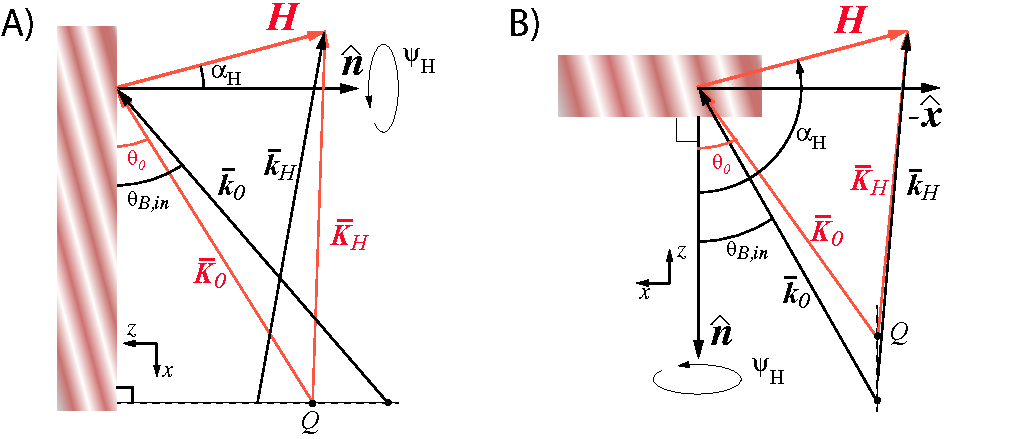
\includegraphics[width=5in]{crystal-diffraction.pdf}
  \caption[Reference trajectory reciprocal space diagram for crystal diffraction.]
{Reference trajectory reciprocal space diagram for for A) Bragg
diffraction and B) Laue diffraction. The bar over the vectors
indicates that they refer to the reference trajectory. The $x$-$z$
coordinates shown are the element surface coordinates. All points in the
diagram are in the plane of the paper except for the tip of $\bfH$.
$\bfKbar_{0}$, and $\bfKbar_{H}$ are the wave vectors inside the
crystal and $\bfkbar_{0}$ and $\bfkbar_{H}$ are the wave vectors
outside the crystal. The reference photon traveling along the
reference trajectory has $\bfKbar_0$ and $\bfKbar_H$ originating at
the $Q$ point. For Laue diffraction, the crystal faces are assumed
parallel.  For Bragg diffraction the crystal normal is in the $-\bfhat
x$ direction while for Laue diffraction the crystal normal is in the
$-\bfhat z$ direction
  }
  \label{f:crystal.diffraction}
\end{figure}

%-------------------------------------------------------------------------
%-------------------------------------------------------------------------
\section{Crystal Element Tracking}
\label{s:crystal.tracking}

\textit{\large [Crystal tracking developed by Jing Yee Chee, Ken Finkelstein, and David Sagan]}

Crystal diffraction is modeled using dynamical diffraction theory. The
notation here follows Batterman and Cole\cite{b:batterman}.  The
problem can be divided up into two parts. First the reference
trajectory must be calculated. This means calculating the incoming
grazing angle $\theta_{B,in}$ and outgoing grazing angle
$\theta_{B,out}$ as well as calculating the transformations between
the various coordinate systems. This is done in \sref{s:crystal.ref},
\sref{s:crystal.trans}, and \sref{s:laue.ref}.  The second part
is the actual tracking of the photon and this is covered in
\sref{s:bragg.track} \sref{s:coherent.laue} and \sref{s:incoherent.laue}.

%-------------------------------------------------------------------------
\subsection{Calculation of Entrance and Exit Bragg Angles}
\label{s:crystal.ref}

\fig{f:crystal.diffraction} shows the geometry of the
problem. The bar over the vectors indicates that they refer to the
reference trajectory. The reference trajectory is calculated such that
the reference photon will be in the center of the Darwin curve. That
is, the internal wave vectors $\bfKbar_0$ and $\bfKbar_H$ originate
from the $Q$ point (See \cite{b:batterman} Figs.~8 and 29).

The external wave vectors $\bf k_0$, and $\bf k_H$ and the internal wave vectors
have magnitude
\begin{align}
  |\bf k_0| &= |\bf k_H| = \frac{1}{\lambda} 
  \label{kk1l1} \\
  |\bfKbar_0| &= |\bfKbar_H| = \frac{1 - \delta}{\lambda}
  \label{kk1l2}
\end{align}
where $\lambda$ is the wavelength, and $\delta$ is
\Begineq
  \delta = \frac{\lambda^2 r_e}{2 \, \pi \, V} \, F_0' = \frac{\Gamma}{2} \, F_0'
  = \frac{1}{2} \, \Gamma \, F_0'
\Endeq
with $r_e$ being the classical electron radius, $V$ the unit cell
volume, and $F_0'$ is the real part of the $F_0$ structure factor. 

In element surface coordinates (which will be the coordinate system used
henceforth), $\bfkbar_0$ lies in the $x$-$z$ plane. $\bfKbar_0$ is
related to $\bfkbar_0$ via Batterman Eq.~(25)
\Begineq
  \bfK_0 = \bfk_0 + q_0 \, \bfhat n
  \label{kkqn1}
\Endeq
where the value of $q_0$ is to be determined. Here, and in equations
below, if the equation is true in general, and not just for the
reference trajectory, the bar superscript is dropped.

Since $\bfhat n$ is in the $-\bfhat x$ direction, $\bfKbar_0$ is also
in the $x$-$z$ plane. Thus $\bfkbar_0$ and $\bfKbar_0$ can be written
in the form
\begin{alignat}{3}
  \bfkbar_0 &= \frac{1}{\lambda} \, 
    \begin{pmatrix}
    -\cos\theta_{B,in} \\
    0 \\
    \sin\theta_{B,in}
    \end{pmatrix}
  \; , & \qquad
  \bfKbar_0 &= \frac{1 - \delta}{\lambda} \, 
    \begin{pmatrix}
    -\cos\theta_0 \\
    0 \\
    \sin\theta_0
    \end{pmatrix}
  & \qquad &\text{[Bragg]} \CRNO
  \bfkbar_0 &= \frac{1}{\lambda} \, 
    \begin{pmatrix}
    \sin\theta_{B,in} \\
    0 \\
    \cos\theta_{B,in}
    \end{pmatrix}
  \; , & \qquad
  \bfKbar_0 &= \frac{1 - \delta}{\lambda} \, 
    \begin{pmatrix}
    \sin\theta_0 \\
    0 \\
    \cos\theta_0
    \end{pmatrix}
  &\qquad & \text{[Laue]} 
  \label{k1lst}
\end{alignat}
Where, as shown in \fig{f:crystal.diffraction}, $\theta_{B,in}$, and
$\theta_0$ are the angles of $\bfkbar_0$ and $\bfKbar_0$ with respect
to the $x$-axis for Bragg reflections and with respect to the $z$-axis
for Laue reflection. 

$\alpha_H$ (\vn{alpha_angle}) is the angle that $\bfH$ makes with
respect to the $-\bfhat z$ axis and $\psi_H$ (\vn{psi_angle}) is the
rotation of $\bfH$ around the $-\bfhat z$ axis such that for $\psi_H =
0$, $\bfH$ is in the $x$-$z$ plane and oriented as shown in
\fig{f:crystal.diffraction}. Thus
\Begineq
  \bfH 
  \equiv \frac{1}{d} \, \bfhat{H} 
  = \frac{1}{d}
    \begin{pmatrix} 
       -\sin \alpha_H \, \cos \psi_H \\ \sin \alpha_H \, \sin \psi_H \\ -\cos \alpha_H
    \end{pmatrix}
  \label{h1daa}
\Endeq
where $\bfhat{H}$ is $\bfH$ normalized to 1. $\alpha_H$ is determined
via the setting of \vn{b_param} and via \Eq{batat}.

The vectors $\bfK_0$ and $\bfH$ must add up to the reciprocal lattice vector $\bfK_H$
\Begineq
  \bfK_H = \bfK_0 + \bfH
  \label{kkh}
\Endeq
Taking the length of both sides of this equation and using
\Eqs{kk1l2}, \eq{k1lst}, and \eq{h1daa} gives for
$\theta_0$
\Begineq
  \sin \theta_0 = 
  \begin{dcases}
    \dsfrac{-\beta \, \what{H}_z - \what{H}_x \, \sqrt{\what{H}_x^2 + \what{H}_z^2 - \beta^2}}
    {\what{H}_x^2 + \what{H}_z^2} & \vn{Bragg} \\
    \dsfrac{-\beta \, \what{H}_x + \what{H}_z \, \sqrt{\what{H}_x^2 + \what{H}_z^2 - \beta^2}}
    {\what{H}_x^2 + \what{H}_z^2} & \vn{Laue}
  \end{dcases}
\Endeq
where
\Begineq
  \beta \equiv \frac{\lambda}{2 \, d \, (1 - \delta)}
\Endeq
Once $\theta_0$ has been calculated, $\theta_{B,in}$ can be calculated from \Eq{kkqn1}
\begin{align}
  \cos\theta_{B,in} &= (1 - \delta) \, \cos\theta_0 \quad [\text{Bragg}] \\
  \sin\theta_{B,in} &= (1 - \delta) \, \sin\theta_0 \quad [\text{Laue}] 
\end{align}

The outgoing reference wave vector $k_H$ is computed using the equation
\Begineq
  \bfK_H = \bfk_H + q_H \, \bfhat n
  \label{kkqn2}
\Endeq
Using this with \Eqs{h1daa} and \eq{kkh} gives
\begin{align}
  \kbar_{H,x} &= \Kbar_{H,z} = \frac{1}{d} \, \what{H}_x + \kbar_{0,x} \CRNO
  \kbar_{H,y} &= \Kbar_{H,y} = \frac{1}{d} \, \what{H}_y 
  \label{k1dapl} \\
  \kbar_{H,z} &= \sqrt{\frac{1}{\lambda^2} - \kbar_{H,x}^2 - \kbar_{H,y}^2} \nonumber
\end{align}

The total bending angle of the reference trajectory is then
\Begineq
  \theta_{bend} = \tan^{-1} 
  \left( \frac{ | \bfkbar_0 \cross \bfkbar_H | }{\bfkbar_0 \dotproduct \bfkbar_H} \right) 
\Endeq
The outgoing Bragg angle $\theta_{B,out}$ is then {\em defined} to be
the difference between the total bend angle and the entrance Bragg angle.
\Begineq
  \theta_{B,out} \equiv \theta_{bend} - \theta_{B,in}
\Endeq

%-------------------------------------------------------------------------
\subsection{Crystal Coordinate Transformations}
\label{s:crystal.trans}

There are four transformations needed between coordinates
denoted by $\Bf\Sigma_1$, $\Bf\Sigma_2$, $\Bf\Sigma_3$, and $\Bf\Sigma_4$
\begin{example}
  \(\Bf\Sigma_1\)  Transform from laboratory entrance to element entrance coordinates.  
  \(\Bf\Sigma_2\)  Transform from element entrance to surface coordinates.  
  \(\Bf\Sigma_3\)  Transform from surface to element exit coordinates.  
  \(\Bf\Sigma_4\)  Transform from element exit to laboratory exit coordinates.  
\end{example}
The total transformation is just the map represented by $\bfS$ and
$\bfV$ of \Eqs{vwlv} and \eq{wws}
\Begineq
  [\bfS, \bfV] = \Bf\Sigma_4 \, \Bf\Sigma_3 \, \Bf\Sigma_2 \, \Bf\Sigma_1
\Endeq

\index{tilt_corr}\index{crystal!tilt correction}
The transformation $\Bf\Sigma_1$ is given in
\sref{s:crystal.trans.le} and the transformation $\Bf\Sigma_4$ is
given in \sref{s:crystal.trans.el}. In general, the transformation
$\Bf\Sigma_1$ needs a ``tilt correction'' (\Eq{tttt}), as explained
below, when $\psi_H$ is nonzero.  [The exception is when the
\vn{undiffracted} or \vn{forward_diffracted} beam is tracked with Laue
geometry. In these cases, no tilt correction is needed.] Since this
tilt correction is independent of any misalignments, the tilt
correction calculation proceeds assuming here that there are no
misalignments. The finite $\bfV$ due to the finite crystal thickness
in Laue diffraction will also be ignored for the moment.

Without misalignments, and with $\psi_H$ zero, the transformation
$\Bf\Sigma_1$ is, as it is for every other type of element,
just the unit matrix. 
\Begineq
  \Bf\Sigma_1 = \bfI
\Endeq
That is, the two coordinate systems are
identical. Furthermore, the transformation $\Bf\Sigma_2$ from element
entrance coordinates to surface coordinates is a rotation around the $y$
axis
\begin{align}
  \Bf\Sigma_2 &= \bfR_y(\theta_{B,in}) \equiv \begin{pmatrix}
     \cos\theta_{B,in} & 0 & \sin\theta_{B,in} \\
     0                 & 1 & 0                 \\
    -\sin\theta_{B,in} & 0 & \cos\theta_{B,in} \\
  \end{pmatrix}
  \qquad &\text{[Laue]}
  \label{mt0t010} \\
  &= \bfR_y(\theta_{B,in} - \frac{\pi}{2})
  \qquad &\text{[Bragg]} \nonumber
\end{align}
The transformation from element surface coordinates to element exit
coordinates, $\Bf\Sigma_3$, is another rotation around the $y$ axis 
\begin{align}
  \Bf\Sigma_3 &= \bfR_y(\theta_{B,out})
  \qquad &\text{[Laue]} \\
  &= \bfR_y(\theta_{B,out} + \frac{\pi}{2})
  \qquad &\text{[Bragg]} \nonumber
\end{align}
and the transformation from element exit coordinates
to laboratory exit coordinates, $\Bf\Sigma_{out}$ is the unity matrix
\Begineq
  \Bf\Sigma_4 = \bfI
\Endeq
Thus, the combined transformation $\bfS$ from laboratory entrance to
laboratory exit coordinates is a rotation around the $y$ axis of
$\theta_{B,in}+\theta_{B,out}$ as explained in section
\sref{s:global}
\Begineq
  \bfS = \Bf\Sigma_4 \, \Bf\Sigma_3 \, \Bf\Sigma_2 \, \Bf\Sigma_1 
  = \bfR_y(\theta_{B,in}+\theta_{B,out})
\Endeq

\index{ref_tilt}\index{psi_angle}
When $\psi_H$ is non-zero, the situation is complicated since, if
$\bfS$ as calculated above is used, the vector $\bfkbar_H$ would be
bent out of the $x$-$z$ plane even though it has been assumed that the
\vn{ref_tilt} $\theta_t$ is zero. But $\bfkbar_H$ points in the same
direction as the $z$ axis of the outgoing reference
trajectory. Furthermore, by {\em definition}, the reference trajectory
has the form given by \Eq{ustt} with the $\bfR_{z}(\theta_t)$ matrix
depending only upon the \vn{ref_tilt} parameter (which is here taken
to be zero). To satisfy \Eq{ustt}, the crystal must be reorientated to
keep the $\bfk_H$ vector in the $x$-$z$ plane of the laboratory
entrance coordinates.  The reorientation is done by rotating the
crystal about the laboratory entrance $\Bf z$ axis by an amount
$\theta_{corr}$ (\vn{tilt_corr}).

With this tilt correction the transformation $\Bf\Sigma_1$ is a
rotation about the $z$ axis
\Begineq
  \Bf\Sigma_1 = 
  \begin{pmatrix}
    \cos\theta_{corr} & -\sin\theta_{corr} & 0 \\
    \sin\theta_{corr} &  \cos\theta_{corr} & 0 \\
    0                 &  0                 & 1                
  \end{pmatrix}
\Endeq
To calculate a value for $\theta_{corr}$, note that
the transformation $\Bf\Sigma_2$ from element entrance coordinates to element surface
coordinates is not affected by a finite $\psi_H$ and so \Eq{mt0t010}
is unmodified. The $\bfk_H$ vector, expressed in laboratory entrance
coordinates, is $\Bf\Sigma_1^{-1} \, \Bf\Sigma_2^{-1} \, \bfk_H$ where the
components of $\bfk_H$ are given by \Eq{k1dapl}. To
satisfy \Eq{ustt}, this vector must have zero $y$ component
\Begineq
  \left( \Bf\Sigma_1^{-1} \, \Bf\Sigma_2^{-1} \, \bfk_H \right) \dotproduct
  \begin{pmatrix} 0 \\ 1 \\ 0 \end{pmatrix}
  = 0
\Endeq
Solving gives
\Begineq
  \theta_{corr} = \tan^{-1} 
  \frac{k_{H,y}}{k_{H,z} \, \sin\theta_{B,in} - k_{H,x} \, \cos\theta_{B,in}}
\Endeq
The transformation $\Bf\Sigma_3$ from element surface coordinates to
element exit coordinates is now obtained by requiring that the total
transformation from laboratory entrance to laboratory exit coordinates
be the $\bfR_{y}(-\alpha_b)$ matrix given in \Eq{ustt}
\Begineq
  \Bf\Sigma_3 \, \Bf\Sigma_2 \, \Bf\Sigma_1 = 
  \begin{pmatrix}
    \cos\theta_{bend} & 0 & -\sin\theta_{bend} \\
    0          & 1 & 0           \\
    \sin\theta_{bend} & 0 & \cos\theta_{bend}
  \end{pmatrix}
\Endeq
In the above equation, the transformation $\Bf\Sigma_4$ has been
dropped since it is the unit matrix independent of $\psi_H$.

For Laue diffraction when the non-diffracted beam is tracked, the exit
coordinate system corresponds to the entrance coordinate system. That
is, $\bfV$ is the unit matrix. In this case, there is no tilt
correction and $\Bf\Sigma_3 = \bfR_y(-\theta_{B,in})$ is just the
inverse of $\Bf\Sigma_2$.

%-------------------------------------------------------------------------

\begin{figure}
\centering
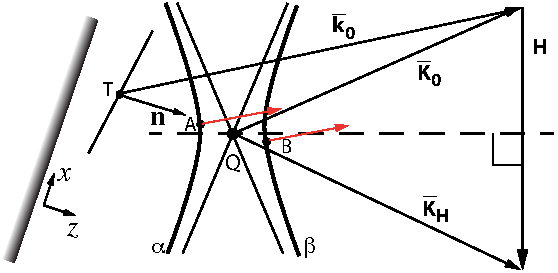
\includegraphics[width=4in]{crystal-energy.pdf}
  \caption[Reference energy flow for Laue diffraction]{
Energy flow used to determine the reference orbit for Laue diffraction.
  }
\label{f:crystal.energy}
\end{figure}

%-------------------------------------------------------------------------
\subsection{Laue Reference Orbit}
\label{s:laue.ref}

For Laue diffraction, with the reference orbit following the
\vn{undiffracted} beam, the reference orbit at the exit surface is
just the extension of the reference orbit at the entrance
surface. Since the reference orbit's direction is $\bfkbar_0$.  the
reference orbit displacement vector $\bfL$ (cf.~\Eq{vwlv}) is given by
\Begineq
  \bfL = \frac{t^2}{d\bfkbar_0 \dotproduct \Bf t} \, d\bfkbar_0
  \qquad \text{[undiffracted]}
\Endeq
where
\Begineq
  \Bf t = \begin{pmatrix}
    0 \\ 0 \\ t
  \end{pmatrix}
\Endeq
with $t$ being the crystal thickness and the $z$-axis pointing into
the crystal as illustrated in \fig{f:crystal.energy}. The $\bfS$
roatation matrix (\Eq{wws}) for the undiffracted beam referece will be
the unit matrix.

With the reference orbit following the \vn{forward_diffracted} or
\vn{Bragg_diffracted} beam, the displacement vector $\bfL$ follows the
energy flow associated with the tie points labeled $A$ or $B$ in
\fig{f:crystal.energy}. These tie points are defined by the
intersection of the dispersion surfaces and the vector $\Bf n$
originating from the point $T$ as shown in the figure.  The energy
flow is perpendicular to the dispersion surface and it can be shown
that since, by construction, $\Bf n$ goes through the $Q$ point and
since the dispersion surfaces are hyperbolies, the energy flow from
$A$ and $B$ tie points are colinear. The direction of the energy flow
is given by:
\Begineq
  \bfKbar_f = \xi_H \, \bfKbar_H + \xi_0 \, \bfKbar_0
\Endeq
$\bfL$ is thus
\Begineq
  \bfL = \frac{t^2}{\bfKbar_f \dotproduct \Bf t} \, \bfKbar_f
\Endeq
where $\Bf t$ is a vector whose length is the thickness of the crystal
oriented perpendicular to the crystal surfaces (that is, in the $z$
direction of the local coordinate system). At the exit surface, if the
reference orbit is following the \vn{forward_diffracted} beam, the
orientation of the \vn{element exit} coordinates will be the same as
the orientation of the \vn{element entrance} coordinates. That is,
$\bfS$ (\Eq{wws}) is the unit matrix.  If the reference orbit is
following the \vn{Bragg diffracted} beam, $\bfS$ is the same as for
Bragg diffraction
\Begineq
  \bfS = 
  \begin{pmatrix}
    \cos\theta_{bend} & 0 & -\sin\theta_{bend} \\
    0                 & 1 & 0           \\
    \sin\theta_{bend} & 0 & \cos\theta_{bend}
  \end{pmatrix}
\Endeq

%-------------------------------------------------------------------------
\subsection{Crystal Surface Reflections and Refractions}

\begin{figure}[tb]
  \centering
  %%%        \includegraphics[width=5in]{crystal-surface-reflect.pdf}
  \caption[Reflection from a crystal surface.]
{Reflection from a crystal surface.}
  \label{f:crystal-reflect}
\end{figure}


There are corrections to the field amplitude and phase when a photon
reflects or refracts from the surface of a crystal. The situation is
illustrated in \fig{f:crystal-reflect}. A plane wave in incident on a
crystal surface with
\Begineq
  E = \what E_0 \, \exp(i \, \bfk_0 \, \bfr)
\Endeq
An outgoing plane wave has a field
\Begineq
  E = \what E_1 \, \exp(i \, \bfk_1 \, \bfr)
\Endeq
A simulation of this condition will start with a number of photons
with wave vector $\bfk_0$ and electric field . After reflecting from
the surface, the photons will have wave vector $\bfk_1$. Now imagine a
set of $N$ photons that flow through an area $dA_0$ before being
reflected from the surface. 

Since the electric field is $\what E_0$, for incoherent photon
tracking
\Begineq
  \what E_0^2 = \frac{\alpha_p \, E_0^2 \, N}{dA_0}
\Endeq
where $\alpha_p$ is the simulation constant (cf.~\Eq{panda1}. 
After the photons are reflected they will have some field $E_1$ and thus
\Begineq
  \what E_1^2 = \frac{\alpha_p \, E_1^2 \, N}{dA_1}
\Endeq
Where $dA_1$ is the area that the phtons flow through which is related
to $dA_0$ via
\Begineq
  \frac{dA_1}{dA_0} = \frac{\bfk_1 \cdot \bfz}{\bfk_0 \cdot \bfz} \equiv |b|
\Endeq
Combining the above three equations, the change in field for a photon
as it reflects from the surface is
\Begineq
  \frac{E_1}{E_0} = \frac{\what E_1}{\what E_0} \, \sqrt{|b|} 
  \qquad \text{Incoherent}
\Endeq

For coherent photon tracking the electric field at $dA_0$ is
\Begineq
  \what E_0 = \frac{\alpha_p \, E_0 \, N}{dA_0}
\Endeq
After the photons are reflected they will have some field $E_1$ and thus
\Begineq
  \what E_1 = \frac{\alpha_p \, E_1 \, N}{dA_1}
\Endeq
Combining these equations the change in field for a photon
as it reflects from the surface is
\Begineq
  \frac{E_1}{E_0} = \frac{\what E_1}{\what E_0} \, |b| 
  \qquad \text{Coherent}
\Endeq

Additionally, for coherent tracking, all photons in a plane wave must
have the same phase when passing through an area transverse to the
wave. Thus the two photons labeled $a$ and $b$ in
\fig{f:crystal-reflect} must have the same phase advance in going from
$dA_0$ to $dA_1$. The difference in the phase advance for photon $b$
relative to $a$ from $dA_0$ to the surface is $\bfk_0 \cdot \bfr$
where $\bfr$ is the vector between where photon $b$ hits the surface
relative to phton $a$. Similarly, the difference in the phase advance
for photon $b$ relative to $a$ from the surface to $dA_0$ is $-\bfk_1
\cdot \bfr$. Since the total phase advance for both photons is the
same from $dA_0$ to $dA_1$ the phase shift $d\phi_b$ of photon $b$ as
it is reflected from the surface relative to the phase shift $d\phi_a$
is
\Begineq
  d\phi_b = d\phi_a - (\bfk_1 - \bfk_0) \cdot \bfr
  \label{dpbdpa}
\Endeq

This shift in the reflection phase can be related to the lattice
diffration planes. The wave vector difference can be writen
\Begineq
  \bfk_1 - \bfk_0 = \bfH + q \, \bfhat n
  \label{k1k0}
\Endeq
where $\bfhat n$ is perpendicular to the surface. Combining
\Eqs{dpbdpa} and \eq{k1k0} and since $\bfr$ is in
the plane of the surface
\Begineq
  d\phi_b = d\phi_a - \bfH \cdot \bfr
\Endeq
This shows that the reflection shift has the same periodicity as the
pattern of the lattice planes at the surface of the crystal. Notice
that for a mirror, where one point on the surface is the same as any
other, $d\phi_b$ must be equal to $d\phi_a$. Using this in \Eq{dpbdpa}
gives 
\Begineq
  \bfk_1 \cdot \bfr = \bfk_0 \cdot \bfr
\Endeq
and since $|\bfk_1| = |\bfk_0|$ this proves that the angle of
incidence is equal to the angle of reflection for a mirror.

In practice, the registration of the surface planes with respect to
the surface is not specified in a simulation. Thus the reflection
phase shift can only be calculated up to a constant offset. 

%-------------------------------------------------------------------------
\subsection{Bragg Crystal Tracking}
\label{s:bragg.track}

The starting photon coordinates are specified in the laboratory
entrance coordinates. The transformation from laboratory entrance
coordinates to element entrance coordinates $\bftilde k_0$ is given in
\sref{s:photon.lab.ele}. The transformation to element surface
coordinates $\bfk_0$ is
\begin{equation}
  \bfk_0 =  \Bf\Sigma_2 \, \bftilde k_0
\end{equation}
with $\Bf\Sigma_2$ given by \Eq{mt0t010}.
The outgoing wave vector $\bfk_H$ is related to $\bfk_0$ via
\Begineq
  \bfk_H =  \bfk_0 + \bfH + q_t \, \bfhat n
\Endeq
where $q_t$ is determined by using \Eqs{k1lst} and \eq{h1daa} in \Eq{kk1l1}
\begin{align}
  k_{H,x} &= k_{0,x} + H_x \nonumber \CRNO
  k_{H,y} &= k_{0,y} + H_y \\
  k_{H,z} &= \sqrt{\lambda^2 - k_{H,x}^2 - k_{H,y}^2} \nonumber
\end{align}

To compute the field amplitude of the outgoing photon, the equation to
be solved is (\cite{b:batterman} Eq.~(21))
\Begineq
  \xi_0 \, \xi_H = \frac{1}{4} \, k^2 \, P^2 \, \Gamma^2 \, F_H \, F_{\bar H}
  \label{xx14}
\Endeq
where $\xi_0$ and $\xi_H$ are given by \cite{b:batterman} Eq.~(18)
and $P$ is the polarization factor
\Begineq
  P = 
  \begin{cases}
    1               & \sigma \text{ polarization state} \\
    \cos 2\theta_g  & \pi \text{ polarization state}
  \end{cases}
\Endeq
$2\theta_g$ is the angle between $\bfK_0$ and $\bfK_H$ which is well
approximated by $\theta_{B,in} + \theta_{B,out}$.

The solution to \Eq{xx14} is (\cite{b:batterman} Eq.~(31))
\begin{align}
  \xi_0 &= \frac{1}{2} \, k \, |P| \, \Gamma \, [F_H \, F_{\bar H}]^{1/2} \, 
    |b|^{1/2} \, [\eta \pm (\eta^2 + \sign(b))^{1/2}] \CRNO
  \xi_H &= \frac{1}{2} \, k \, |P| \, \Gamma \, [F_H \, F_{\bar H}]^{1/2} \, 
    \frac{1}{|b|^{1/2} \, [\eta \pm (\eta^2 + \sign(b))^{1/2}]}
\end{align}
where the $+$ part of $\pm$ is for the $\alpha$ branch and the $-$
part of $\pm$ is for the $\beta$ branch and $\sign$ is the sign
function
\Begineq
  \sign(b) \equiv \begin{cases} 1 & b > 0 \\ -1 & b < 0 \end{cases}
\Endeq
and $\eta$ is given by \cite{b:blasdell} Eq.~(5)
\Begineq
  \eta = \frac{-b \, a + \Gamma \, F_0 \, (1 - b)}{2 \, \Gamma \, |P| \, \sqrt{|b| \, F_H \, F_{\bar H}}}
\Endeq
with the asymmetry factor $b$ for the photon being tracked being given
by \cite{b:blasdell} Eq.~(3)
\Begineq
  b \equiv \frac{\bfhat n \dotproduct \bfhat k_0}{\bfhat n \dotproduct (\widehat{{\bfk_0 + \bfH}})}
\Endeq
and the angular deviation variable $a$ is given by \cite{b:blasdell} Eq.~(4)
\Begineq
  a \equiv \frac{H^2 + 2 \, \bfk_0 \dotproduct \bfH}{k_0^2} 
  = -2 \, \Delta \theta \, \sin(2\theta_B)
\Endeq
Once $\xi_0$ and $\xi_H$ are determined, the ratio of the incoming and outgoing fields
for the $\alpha$ or $\beta$ branches can be computed via (\cite{b:batterman} Eq.~(24))
\Begineq
  r_E \equiv \frac{\bfE_H}{\bfE_0} 
  = \frac{- \, 2 \, \xi_0}{k \, P \, \Gamma \, F_{\bar H}} \,
  = \, \frac{- \, k \, P \, \Gamma \, F_H}{2 \, \xi_H} 
\Endeq
where the $\alpha$ or $\beta$ subscript has been supressed.  The total
field which is the sum of the fields on the branches is computed using
the boundary conditions
\Begineq
  \bfE_0 = \bfE_{0\alpha} + \bfE_{0\beta}, \qquad\qquad 
  0 = \bfE_{H\alpha} + \bfE_{H\beta}
\Endeq
Using the above two equations gives
\begin{align}
  \bfE_{0\alpha} &= \bfE_0 \, \frac{r_{E\beta}}{r_{E\beta} - r_{E\alpha}} \qquad\qquad
  \bfE_{H\alpha}  = \bfE_0 \, \frac{r_{E\alpha} \, r_{E\beta}}{r_{E\beta} - r_{E\alpha}} \CRNO
  \bfE_{0\beta} &= -\bfE_0 \, \frac{r_{E\alpha}}{r_{E\beta} - r_{E\alpha}} \qquad\qquad
  \bfE_{H\beta}  = -\bfE_0 \, \frac{r_{E\alpha} \, r_{E\beta}}{r_{E\beta} - r_{E\alpha}} 
\end{align}

As can be seen from Battermann and Cole Figs.~(8) and (29), the
$\alpha$ tie point is excited and the $\beta$ tie point is not if
$\xi_{0\alpha} < \xi_{0\beta}$ and vice versa. Since only one tie
point is excited, The external field ratio is equal to
the internal field ratio 
\Begineq
  \frac{E_H^e}{E_0^i} = \frac{E_{Hj}}{E_{0j}}
\Endeq
where $j$ is $\alpha$ or $\beta$ as appropriate.

%-------------------------------------------------------------------------
\subsection{Coherent Laue Crystal Tracking}
\label{s:coherent.laue}

Laue diffraction has two interior wave fields (branches), labeled
$\alpha$ and $\beta$, corresponding to the two tie points that are
excited on the two dispersion surfaces. For coherent tracking, a
photon has some probability to be channeled to follow the $\alpha$ or
$\beta$ branch. The electric field ratios $\what E_\alpha$ and $\what
E_\beta$ (cf.~\Eq{rpss2}) are taken to be equal to each other. With
this choice, the probabilities $P_\alpha$ and $P_\beta$ for being
channeled to the $\alpha$ or $\beta$ branches are such that a branch
with a greater intensity will have a greater number of photons
chanelled down it.

When a crystal's \vn{ref_orbit_follows} parameter is set to
\vn{bragg_diffracted}, The branching probabilities are
\Begineq
  P_\alpha = \frac{|E_{H\alpha}|}{|E_{H\alpha}| + |E_{H\beta}|} , \qquad
  P_\beta = \frac{|E_{H\beta}|}{|E_{H\alpha}| + |E_{H\beta}|} , \qquad
  \what E_{H\alpha} = \what E_{H\beta}  = \frac{|E_{H\alpha}| + |E_{H\beta}|}{|E_0^i|}
\Endeq
where (see Batermann and Cole\cite{b:batterman} Eqs~(42)), 
\begin{align}
  E_{H\alpha} &= -E_0^i \, \dsfrac{|b|^{1/2}}{2 \, \cosh v} \, 
    \frac{|P|}{P} \, 
    \frac{[F_H \, F_\Hbar]^{1/2}}{F_H} \, 
    \exp({-2 \, \pi \, i \, \bfK'_{H\alpha} \dotproduct \bfr_\alpha}) \,
    \exp({-2 \, \pi \, \bfK''_{H\alpha} \dotproduct \bfr_\alpha}) \CRNO
  E_{H\beta} &= E_0^i \, \dsfrac{|b|^{1/2}}{2 \, \cosh v} \, 
    \frac{|P|}{P} \, 
    \frac{[F_H \, F_\Hbar]^{1/2}}{F_H} \, 
    \exp({-2 \, \pi \, i \, \bfK'_{H\beta} \dotproduct \bfr_\beta}) \,
    \exp({-2 \, \pi \, \bfK''_{H\beta} \dotproduct \bfr_\beta})
\end{align}
where $\bfr_\alpha$ and $\bfr_\beta$ are the vectors from the
entrance surface to the exit surface for the $\alpha$ and $\beta$ wave
fields
\Begineq
  \bfr_\alpha = \frac{t^2}{\bfS_\alpha \dotproduct \Bf t} \, \bfS_\alpha , \qquad
  \bfr_\beta = \frac{t^2}{\bfS_\beta \dotproduct \Bf t} \, \bfS_\beta
\Endeq
with
\begin{align}
  \bfS_\alpha &= e^{-2 \, v} \, \Bf s_0 + \left| b \, \frac{F_H \, F_\Hbar}{F_H^2} \right| \, \Bf s_H \CRNO
  \bfS_\beta &= e^{2 \, v} \, \Bf s_0 + \left| b \, \frac{F_H \, F_\Hbar}{F_H^2} \right| \, \Bf s_H 
\end{align}
The phase shift of the electric field is obtained from the phase of
$E_{H\alpha}$ if the photon is channeled into the $\alpha$ branch and
$E_{H\beta}$ if the photon is channeled into the $\beta$ branch.

When a crystal's \vn{ref_orbit_follows} parameter is set to
\vn{forward_diffracted} or \vn{undefracted}, the algorithm is similar
to the \vn{bragg_diffracted} case except $E_{0\alpha}$ and
$E_{0\beta}$ are used in place of $E_{H\alpha}$ and
$E_{H\beta}$ with
\begin{align}
  E_{0\alpha} &= E_0^i \, \dsfrac{e^{-v}}{2 \, \cosh v} \, 
    \exp({-2 \, \pi \, i \, \bfK'_{0\alpha} \dotproduct \bfr_\alpha}) \,
    \exp({-2 \, \pi \, \bfK''_{0\alpha} \dotproduct \bfr_\alpha}) \CRNO
  E_{0\beta} &= E_0^i \, \dsfrac{e^{-v}}{2 \, \cosh v} \, 
    \exp({-2 \, \pi \, i \, \bfK'_{0\beta} \dotproduct \bfr_\alpha}) \,
    \exp({-2 \, \pi \, \bfK''_{0\beta} \dotproduct \bfr_\beta})
\end{align}

Since a simulation photon has two polarization components, the above
equations are used for one polarization component and for the second
polarization component the same branch is used as for the first with
an appropriately scaled $\what E$.

%-------------------------------------------------------------------------
\subsection{Incoherent Laue Crystal Tracking}
\label{s:incoherent.laue}

Laue diffraction has two interior wave fields (branches), labeled
$\alpha$ and $\beta$, corresponding to the two tie points that are
excited on the two dispersion surfaces. For incoherent tracking it is
assumed that these wave fields overlap at the exit surface
(\cite{b:batterman} Eq.~(87)) and so add coherently. This is a good
approximation if the crystal is very thin where the wave fields do not
travel an appreciable spatial distance and is also a good
approximation when the crystal is thick since the $\beta$ branch will
be heavily attenuated. At intermediate thicknesses this approximation
is good when a photon is near the Bragg angle since, in this case, the
fields will be traveling in similar directions.

Another approximation is that the path

\begin{align}
  E_{H\alpha} &= -E_0^i \, \dsfrac{|b|^{1/2}}{2 \, \cosh v} \, 
    \frac{|P|}{P} \, 
    \frac{[F_H \, F_\Hbar]^{1/2}}{F_H} \, 
    \exp({-2 \, \pi \, i \, \bfK'_{H\alpha} \dotproduct \bfr_\alpha}) \,
    \exp({-2 \, \pi \, \bfK''_{H\alpha} \dotproduct \bfr_\alpha}) \CRNO
  E_{H\beta} &= E_0^i \, \dsfrac{|b|^{1/2}}{2 \, \cosh v} \, 
    \frac{|P|}{P} \, 
    \frac{[F_H \, F_\Hbar]^{1/2}}{F_H} \, 
    \exp({-2 \, \pi \, i \, \bfK'_{H\beta} \dotproduct \bfr_\beta}) \,
    \exp({-2 \, \pi \, \bfK''_{H\beta} \dotproduct \bfr_\beta})
\end{align}


%-------------------------------------------------------------------------
\section{X-ray Targeting}
\label{s:targeting}

X-rays can have a wide spread of trajectories resulting in many
``doomed'' photons that hit apertures or miss the detector with only a
small fraction of ``successful'' photons actually contributing to the
simulation results. The tracking of doomed photons can therefore
result in an appreciable lengthening of the simulation time. To get
around this, \bmad can be setup to use what is called ``targeting'' to
greatly reduce the number of doomed photons generated.

Photons can be generated either at a source like a \vn{wiggler}
element or at a place where diffraction is simulated like at a
\vn{diffraction_plate} element. To be able to do targeting, an element
with apertures defined must be present downstream from the generating
element. The idea is to only generate photons that are going in the
general direction of the ``target'' which is the space within the
aperture.

A necessary restriction for
targeting to work is that the photon must travel in a straight line
through all elements between the generating element and the element
with the apertures. So, for example, a \vn{crystal} element would not
be allowed between the two two elements. A \vn{crystal} element could
be the aperture element as long as the aperture was defined before
photons were diffracted. That is, if the aperture was at the upstream
end of the crystal or was defined with respect to the \vn{crystal}
surface.

The target is defined by the four corners of the aperture. In \vn{element}
coordinates, the $(x, y, z)$ values of the corners are:
\begin{example}
  (-x1_limit, -y1_limit, z_lim)
  (-x1_limit,  y2_limit, z_lim)
  ( x2_limit, -y1_limit, z_lim)
  ( x2_limit,  y2_limit, z_lim)
\end{example}
where \vn{x1_limit}, etc. are the the aperture limits (\sref{s:limit})
and \vn{z_lim} will be zero except if the element's \vn{aperture_at}
parameter is set to \vn{entrance_end} in which case \vn{z_lim} will be set
to \vn{-L} where \vn{L} is the length of the element. 

If the aperture is associated with a curved surface (for example with
a \vn{crystal} element), four extra corner points are also used to
take into account that the aperture is not planer. These extra points
have $(x, y, z)$ values in \vn{element} coordinates of
\begin{example}
  (-x1_limit, -y1_limit, z_surface(-x1_limit, -y1_limit))
  (-x1_limit,  y2_limit, z_surface(-x1_limit,  y2_limit))
  ( x2_limit, -y1_limit, z_surface( x2_limit, -y1_limit))
  ( x2_limit,  y2_limit, z_surface( x2_limit,  y2_limit))
\end{example}
where \vn{z_surface(x,y)} is the $z$ value of the surface at the
particular $(x, y)$ point being used. Notice that in this case
\vn{z_lim} is zero.

The coordinates of the four or eight corner points are converted from
\vn{element} coordinates of the aperture element to \vn{element}
coordinates of the photon generating element. Additionally,
the approximate center of the aperture, which in \vn{element}
coordinates of the aperture element is $(0, 0, z_lim)$, is converted
to \vn{element} coordinates of the photon generating element.

The above calculation only has to be done once at the beginning of a
simulation.

When a photon is to be emitted from a given point $(x_{emit},
y_{emit}, z_{emit})$, the problem is how to restrict the velocity
vector $(\beta_x, \beta_y, \beta_z)$ (which is normalized to 1) to
minimize the number of doomed photons generated. The problem is solved
by constructing a vector $\Bf r$ for each corner point:
\Begineq
  \Bf r = (x_{lim}, y_{lim}, z_{lim}) - (x_{emit}, y_{emit}, z_{emit})
\Endeq 
The direction of each $\Bf r$ is characterized in polar coordinates
$(\phi, y)$ defined by
\begin{align}
  y &= \frac{r_y}{|r|} \CRNO
  \tan\phi &= \frac{r_x}{r_z} 
\end{align}
For now make the assumption that $r_z$ is positive and larger than
$r_x$ and $r_y$ for all $\Bf r$.  Let $\phi_{max}$ and $\phi_{min}$ be
the maximum and minimum $\phi$ values over all the $\Bf r$. Similarly,
let $y_{min}$ and $y_{max}$ be the minimum and maximum $y$ values over
all the $\Bf r$. The rectangle in $(\phi, y)$ space defined by these
four min and max values almost covers the projection of the aperture
onto the unit sphere. There is a correction that must be made due to
the fact that a straight line of constant $y$ in $(x, y, z)$ space
projects to a curved line when projected onto $(\phi, y)$
space. Therefore a correction must be made to $y_{min}$ when $y_{min}
< 0$:
\Begineq
  y_{min} \rightarrow 
  \frac{y_min}{\sqrt{(1 - y_{min}^2) \, \cos^2 (phi_{max} - \phi_{min})/2 + y_{min}^2}}
\Endeq
with a similar correction for $y_{max}$ that must be made when $y_{max} > 0$.


The above prescription works as long as the projection of the aperture
onto $(\phi, y)$ space does not touch the branch cut at $\phi = \pi$
or cover the singular points $y = \pm 1$. Generally these restrictions
are fullfilled since $\Bf z$ is the direction of the reference
orbit. If this is not the case, a transformation can be made where
rotation matrices are constructed to transform between the
\vn{element} coordinates of the emitting element and what are called
\vn{target} coordinates defined so that $\Bf r$ for the \vn{center} point
has the form $(0, 0, |r|)$. The procedure for calculating the photon
velocity vector is now
  \begin{enumerate}
  \item
Rotate all the corner $\Bf r$ from \vn{element} to \vn{target} coordinates.
  \item
Calculate min and max values for $\phi$ and $y$.
  \item
Calculate the velocity vector such that the $(\phi, y)$ of this vector
falls within the min and max values in the last step.
  \item
Rotate the velocity vector back to \vn{element} coordinates.
  \end{enumerate}


\chapter{Simulation Modules}

In the \bmad ``ecosystem'', various modules have been developed to
simulate machine hardware. This chapter provides documentation.

%-----------------------------------------------------------------
\section{Tune Tracker Simulator}
\index{tune tracker simulation}

\textit{\large [Tune tracker simulation developed by Michael Ehrlichman]}

The digital tune tracker (dTT) is device for determining the
fractional tune of a storage ring and exciting resonant beam
oscillations.  In short, the dTT starts with a beam position monitor
(BPM) to detect the beam oscillations. The signal from the BPM is feed
into a phase-locked loop (PLL) circuit which oscillates at the
oscillation frequency the beam. A signal from the PLL is used to
modulate a kicker to keep the beam oscillating at the beam's
oscillation frequency. The tune tracker is capable of exciting both
betatron and synchrotron oscillations.

In general, a PLL is a control system for matching the frequency of a
VCO to some incoming periodic reference signal.  It does this by
adjusting the frequency of the VCO according to the phase difference
between the VCO output and the reference signal.  A general diagram of
a PLL is shown in \fig{f:PLL}.

  \begin{figure}[bt]
  \centering
  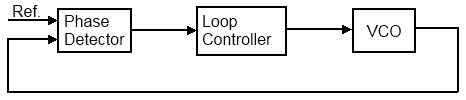
\includegraphics{PLL.png}
  \caption[General diagram of a phase lock loop.]{
General diagram of a phase lock loop. The loop adjusts the speed of a
VCO according to the phase difference between the VCO and an incoming
signal.}
  \label{f:PLL}
  \end{figure}

In \fig{f:PLL}, the phase detector compares the two incoming
signals, and outputs a signal that is proportional to the difference
in phase.  There are various ways to implement a phase detector.  The
tune tracker phase detector is a mixer followed by low-pass filter,
which will be discussed in more detail below.  The loop controller,
also known as a loop filter, is usually some combination of
(P)roportional, (I)ntegration, and (D)ifferentiation paths.  The loop
controller sums these paths, and the resulting signal is sent to the
VCO.  The output of the loop controller rises when the VCO is slower
than the reference, and drops when the VCO is faster.  The gains of
the three PID paths are adjusted to produce a control loop that is
stable and can efficiently lock onto the reference signal from some
incorrect initial frequency.  A real-world PLL also needs to track
perturbations to the reference frequency.

A diagram of the digital tune tracker is shown in
\fig{f:CdTT}.  This function takes in one new BPM measurement
per call, and returns a sinusoidal signal that has the same frequency
as the BPM signal.  The phase of the returned signal differs from the
phase of the BPM signal by $\phi_0$, the phase advance from position
at the BPM to position at the kicker on the next turn.

Comparing this diagram to the PLL in \fig{f:PLL}, the boxes
from {\it Subtract closed orbit offset} to the end of the {\it Low
Pass Filter} comprise the phase detector.  After the {\it Low Pass
Filter} to just before the {\it Gain Kvco} box comprises the loop
controller.  The {\it Gain Kvco} box comprises the VCO.  The feedback
loop consists of the update to $\omega$ that follows {\it Gain Kvco}.

\begin{sidewaysfigure}[tb]
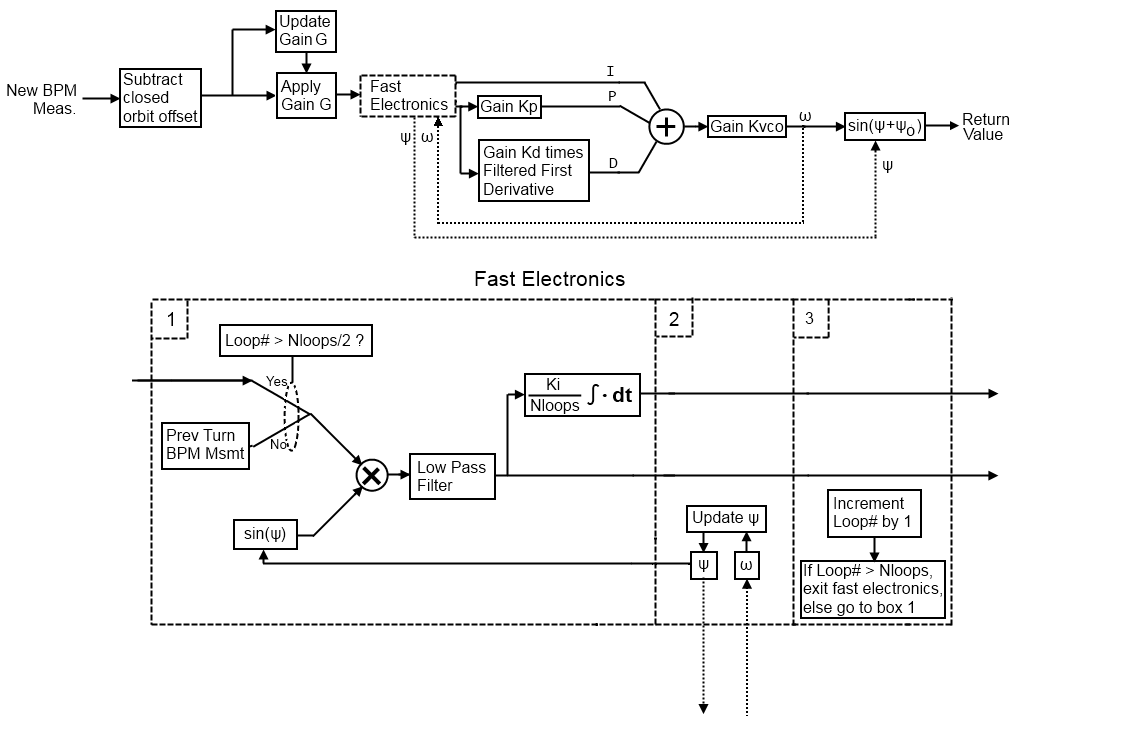
\includegraphics[width=\columnwidth]{TT-Flow.png}
\caption{
Flow chart of tune tracker module functions.}
\label{f:CdTT}
\end{sidewaysfigure}

\clearpage

\subsection{Tune Tracker Components.}
\begin{description}
\item[New BPM Meas.]  
This consists of one BPM measurement.  It is either horizontal or
vertical position at the BPM location.  It is assumed that each
measurement is separated by the same $\Delta t$, and that $\Delta t$
is an integer multiple of the ring period.

\item[Subtract closed orbit offset]  
Due to misalignments or the presence of wigglers, the closed orbit at
the BPM may be non-zero.  The closed orbit is subtracted from the
incoming data.  The closed orbit offset is a constant parameter set by
the user during initialization.

\item[Apply Gain G]  This block adjusts the incoming measurement such that,
\begin{equation*}
Meas.\ Out = \frac{Meas.\ In}{G}
\end{equation*}
The purpose of this block is to normalize the BPM measurements.  When
the tune tracker first starts, the amplitude of the beam oscillations
is small.  When the tune tracker is locked on, the amplitude of the
beam oscillations becomes large.  The set of loop controller gains
that allows the tune tracker to quickly lock onto the initially small
signal are not optimal when the beam oscillations are large.  This
normalization overcomes that problem, allowing for a set of loop
controller gains that are optimal both at start up and when
oscillations are large.

\item[Update Gain G]  This is a digital filter of the form,
\begin{equation*}
G = g_a \textrm{abs}\left(x\right) + \left(1-g_a\right)G\textrm{,}
\end{equation*}
which is a exponentially weighted moving average, or equivalently, a
low-pass filter.  $x$ is the incoming data point.  $g_a$ is a
hard coded time constant.  It is set so that $G$ equilibrates to the
rms beam size after about 10 periods.

\item[Fast Electronics]  
Fast electronics contains the components of the tune tracer that cycle
every few RF periods.  Whereas the rest of the tune tracker cycles
once per storage ring period, the fast electronics cycle every few RF
buckets.

\item[Prev Turn BPM Msmt]  Stores the previous turn's BPM measurement.

\item[Loop\# $\boldsymbol >$ $\boldsymbol N_{loops}/2$ ?]  
$N_{loops}$ is the number of times the fast electronics cycle every
storage ring period.  For the first half of these loops, the BPM
measurement from the previous turn is used.  For the last half, the
current BPM measurement is used.

\item[$\boldsymbol \sin\left(\psi\right)$]  
Sinusoid of the current modulator angle $\psi$.

\item[$\boldsymbol \psi$]  
Current modulator angle.  Updated at the end of every fast electronics loop.

\item[$\boldsymbol \times$ (times)]  
The BPM measurement and $\sin\left(\psi\right)$ are multiplied.  
Let the BPM signal be parameterized as $\cos\left(\omega_{beam}t\right)$, and 
write $\psi$ as $\omega_{vco}t$ so we have,
\begin{equation*}
\cos\left(\omega_{beam}t\right)\sin\left(\omega_{vco}t\right)\textrm{.}
\end{equation*}
A trig identity allows this to be written as,
\begin{equation*}
\frac{1}{2}\left(\sin\left(\left(\omega_{beam}+\omega_{vco}\right)t\right)-
\sin\left(\left(\omega_{beam}-\omega_{vco}\right)t\right)\right)\textrm{.}
\end{equation*}
If $\omega_{vco}$ is roughly $\omega_{beam}$, then the first $\sin$
term has roughly twice the beam frequency and the second term has a
very small frequency.  Therefore, passing the multiplied signal
through a low-pass filter removes the first term, leaving only the
second term.

In stable operation, $\omega_{vco}$ makes small amplitude oscillations
about $\omega_{beam}$.  In this case, the time integral of
$\left(\omega_{beam}-\omega_{vco}\right)t$ is small for all $t$, and a
small angle approximation for sine can be applied, and the output of
the low pass filter can be written as,
\begin{equation}
\left(\omega_{beam}-\omega_{vco}\right)t\textrm{,}
\end{equation}
which is proportional to the phase difference between the beam and the VCO.  Thus completes
the phase detector.

\item[$\boldsymbol{\frac{K_I}{N_{loops}}\int\cdot dt}$]  
This is the (I)ntegrated channel of the PID controller.  It integrates
the output of the phase detector, providing negative feedback.  If the
integrated phase is positive, the I channel slows the VCO down.  If
negative, it speeds the VCO up.  This channel is expected to
equilibrate to some non-zero value proportional to the difference
between the beam frequency and the VCO base frequency.

\item[Update $\boldsymbol{\psi}$] This increments the modulator phase according to,
\begin{equation}
\psi_{n+1}=\psi_n+\frac{T_{ring}}{N_{loops}}\omega_{vco}\textrm{.}
\end{equation}
In order to more accurately model things,
$\omega_{vco}$ is not updated within the fast electronics loop.

\item[Increment Loop\# by 1]  
Loop\# counts the number of times the fast electronics has been looped
through.

\item[If Loop\# $>$ $N_{loops}$, exit, else, loop]  
$N_{loops}$ is the number of times the fast electronics cycle per ring
period.

\item[Gain $\boldsymbol K_P$] 
This is the (P)roportional channel of the PID controller.  Is provides
negative feedback proportional to the output of the phase detector.
This channel responds faster than the integrated channel and so helps
the tune tracker track sudden changes in the frequency of the beam.
In practice, it also damps tune tracker oscillations.  If $K_P$ is too
small, the VCO may oscillate indefinitely around the fractional tune
of the beam.  See section~\sref{Tuning} below for more details.

\item[Gain $K_D$ $\times$ filtered derivative]  
This is the (D)ifferential channel of the PID controller.  Provides a
filtered first derivative of the output of the phase detector.  The
derivative is obtained a polynomial fitted to a history of the phase
detector output.  This channel can be used to smooth out the VCO
response and reduce overshoot.  See section~\sref{Tuning} below for
more details.

\item[$\boldsymbol +$ (sum)]  
This block sums the three output of the PID controller.

\item[Gain $K_{vco}$] 
This block represents the response of a voltage controlled oscillator.
The frequency of the output of a VCO is proportional to the voltage of
its input.  This block simply multiplies the output of the PID
controller by a constant.  This block updates the VCO frequency.

\item[$\boldsymbol{\sin\left(\psi+\psi_0\right)}$]  
Calculates kicker amplitude to be returned to the calling program.
This is the kick amplitude that should be used during the next turn.
$\psi_0$ is the phase advance from position at the BPM to position at
next turn's kicker.

\end{description}

\subsection{Tuning \label{Tuning}} Tuning the tune tracker consists of
adjusting the four gain parameters $K_P$, $K_I$, $K_D$, and $K_{vco}$.
The goal is to set the parameters such that the tune tracker quickly
locks onto the fractional tune of the beam, and settles quickly.  If
multiple tunes are being explored, then the size of the convergence
region is also important.  i.e.  The set of parameters should work for
a wide range of fractional tunes.  If jitter is being explored, then
the ability of the tune tracker to track a varying fractional tune is
also important.

A plot of the VCO speed during typical tune tracker operation is shown
in \fig{f:typ-tt}.  A tune tracker with a base period of 0.571
oscillations per ring period tracks a beam with a fractional tune of
0.5691.  Marked on this plot are 4 important features.  They are the
rise time, overshoot, settling rate, and precision.  The rise time is
how long it takes the tune tracker to approach the fractional tune of
the beam.  This is the location of the first peak after operation
begins.  The overshoot is the difference between the amplitude of the
first peak and the fractional tune.  The settling rate measures the
decay rate of the oscillations of the VCO about the fractional tune.
The precision is the noise in the VCO frequency.  The discrete nature
of the BPM measurements introduces noise at the phase detector stage.
The proportional channel adds this noise to the VCO frequency Shown in
Tab.~[\ref{t:pid-params}] is the effect increasing the PID controller
gains.

\begin{table}
\begin{tabular}{llllll} \toprule
Parameter&  Rise Time&        Overshoot&        Settling Rate&      Precision&  Stability Region\\ \midrule
$K_P$&      slight decrease&  decrease&         faster&             degrade&    shrink\\
$K_I$&      decrease&         increase&         slower&             no change&  shrink\\
$K_D$$^\textrm{see note}$&    slight increase&  slight decrease&  slightly faster&    degrade&    grow\\ \bottomrule
\end{tabular}
\caption[Effect on VCO response of increasing $K_P$, $K_I$, or $K_D$.]{
Effect on VCO response of increasing $K_P$, $K_I$, or $K_D$. 
{\it Note:} The effects of the derivative channel are theoritical and have not 
been verified extensively.}
\label{t:pid-params}
\end{table}

Stability region refers to the range of fractional tunes that the tune
tracker will converge to when starting from an initial tune in that
range.  In practice, if $K_P$ and $K_I$ are increased to optimize
response to a particular fractional tune, the the stability region
will shrink.  e.g.  A large $K_P$ and $K_I$ could be found that very
quickly lock on to a fractional tune of 0.569, but are unstable for
0.622.  But note that a smaller $K_P$ and $K_I$ can be found that give
acceptible performance at 0.569, and also acceptible performance at
0.622 (and even 0.074).

\begin{figure}[tb]
\centering
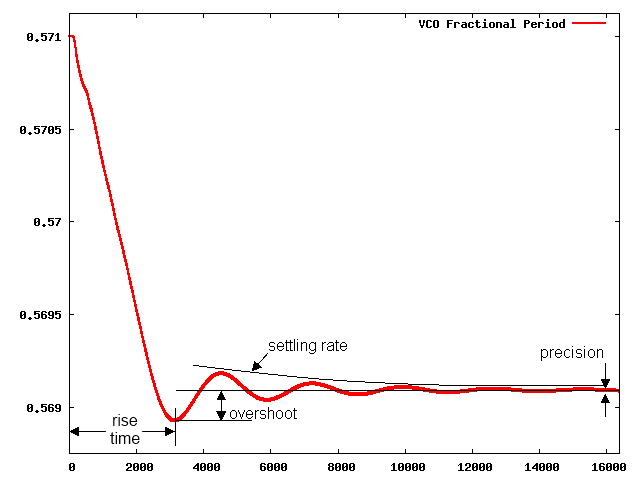
\includegraphics[scale=0.75]{vco_plot.png}
\caption[Plot of VCO response of typical tune tracker setup.]{
Plot of VCO response of typical tune tracker setup.  VCO base frequency is 0.571.
Beam fractional tune is 0.5691.}
\label{f:typ-tt}
\end{figure}

%----------------------------------------------------------------------

\subsection{Programmer Instructions}

This seciton contains instructions on how to implement the tune
tracker module and how to use the tune tracker driver program.  The
tune tracker is written as an object or class, and so supports
multiple instances.

After setting up the tune tracker in a program, it is best to first
verify that the tune tracker is efficiently locking onto the beam and
that the beam oscillations are indeed growing with time.  The tune
tracker should lock on after about 10,000 turns, and the beam
oscillations should reach equilibrium amplitude after about 10 damping
periods.

See the tune tracker section in the Physics chapter of this manual for
an example of how the VCO frequency should respond with time in a
successful implementation.  Guidelines for setting the gain parameters
are also located in the Physics chapter.

%-------------------------------------------------------------------------
\subsection{Tune Tracker Module}

The tune tracker module has four public functions.  They are,
\begin{alltt}
Function id = init_dTT(tt_param_struct)     !Constructor, creates new tune tracker 
                                            !instance, handles initialization.
                                            !Passed tt_param_struct, Returns id of 
                                            !created instance.
Function z = TT_update(bpm_msmt,id)         !Main function, passed one new BPM 
                                            !measurement and returns VCO modulator 
                                            !amplitude.
Subroutine dest_dTT(id)                     !Destructor, closes log files and 
                                            !deallocates memory.
                                            !Takes as argument id of instance 
                                            !to be destroyed.
Function z = get_dTT(name,id)               !Get function, name is either 'wf', 
                                            !in which case the function returns 
                                            !the VCO frequency \(\omega0+\Delta\omega\), 
                                            !or 'dw', in which case just \(\Delta\omega\)
                                            !is returned.
\end{alltt}

Pseudocode for a tune tracker implementation is below.
\begin{verbatim}
Populate tt_param_struct with tune tracker parameters.
id = init_dTT(tt_param_struct)
Loop over turns:
  Track once through the ring, obtain orbit.
  bpm_msmt = x or y at BPM location.
  z = TT_update(bpm_msmt,id)
  Adjust kicker amplitude (or cavity phase) according to z
dest_dTT(id)
\end{verbatim}

See {\tt tune\_tracker.f90} for the contents of {\tt tt\_param\_struct}.

If a horizontal or vertical tune tracker is to be implemented, the BPM
measrements should be the $x$ or $y$ coordinate at the BPM location,
and the kicks should be changes in $x'$ or $y'$ at the kicker
location.  If a longitudinal tune tracker is to be implemented the BPM
measurements should be the $x$ coordinate in a dispersive region, and
the kicks should be changes in phase at an RF cavity.  Similarly, if a
longitudinal tune tracker is being used in conjunction with a
horizontal tune tracker, the BPM of the horizontal tune tracker should
be placed in a region of low dispersion.  This will prevent the
horizontal tune tracker from inadvertantly locking onto the
synchrotron tune.

%-----------------------------------------------------------
\subsection{Tune Tracker Example Program}

An example program is located in {\tt
src/examples/tune\_tracker}. This program contains code for
implementing simultaneous horizontal, vertical, and longitudinal tune
trackers.

For most implementations of the tune tracker module, a good approach
would be to either use a modified version of the tune tracker example
program, or copy and paste code from the example program.  Keep in
mind that the example program implements multiple simultaneous tune
trackers.  An implementation of just one tune tracker would be much
simpler.

The example program performs the following steps.
\begin{enumerate}
\item 
Read in file which contains tune tracker parameters such as gains.
\item 
Parse lattice with {\tt twiss3} subroutines.  The {\tt twiss3} subroutines
are needed to obtain the longitudinal phase advance when implementing 
longitudinal tune trackers.
\item 
Check that the kick attribute of the kicker element is actually free.
\item 
Calculate phase advance from position at BPM to position at kicker.  Note that this 
is the phase of the kicker {\it on the next turn}.
\item 
Creates log files which record position at BPM and kicker, the VCO frequency,
and slope at the kicker.
\item
Loops over turns, passing BPM measurements to {\tt TT\_update} and
adjusting kicker amplitudes based on the returned value.  Note that it
will take the beam oscillations several damping times to equilibriate.
This often means tracking for several 10,000 turns.  Use of the save
state parameter may shorten simulation times in certain applications.
\item 
Calculates and FFT of the BPM data and records in log file. 
\end{enumerate}

Also located in {\tt src/examples/tune\_tracker} is an example .in
file that implements horizontal, vertical, and longitudinal tune
trackers.  The gains used in the .in file were selected for their
large convergence region.  More agressive tuning may lead to faster
lock on.  See the Physics section for details.

%----------------------------------------------------------------------------
\subsection{Save States}

If {\tt tt\_param\_struct\%useSaveState} is set to true, then the
destructor {\tt dest\_dTT} will save the tune tracker state variables
to a file called {\tt tt\_state.\#}.  Similarly, the constructor {\tt
init\_dTT} will set the state variables according to the save state
file.  The constructor will also return the beam coordinates to be
used at element zero of the ring.

Save states allow you to pick up where you left off, and not have to
wait for the beam oscillations to equilibriate.  For example, you
could have one program that tracks for 100,000 turns, allowing the
tune tracker to lock on and the beam excitation to equilibriate with
radiation damping.  The simulation writes a save state file which can
be used as a starting point for other simulations that perform studies
on the excited beam.

%-----------------------------------------------------------------
\section{Instrumental Measurements}
\label{s:meas.calc}
\index{measurement}

\bmad has the ability to simulate instrumental measurement errors
for orbit, dispersion, betatron phase, and coupling measurements.
The appropriate attributes are listed in \sref{s:meas.attrib} and
the conversion formulas are outlined below.

%-----------------------------------------------------------------
\subsection{Orbit Measurement}
\index{orbit!measurement}

For orbits, the
relationship between measured position $(x, y)_{\text{meas}}$ and true position 
$(x, y)_{true}$ is
\Begineq
  \begin{pmatrix}
    x \\
    y
  \end{pmatrix}_{\! \text{meas}}
  =
  n_f \, 
  \begin{pmatrix}
    r_1 \\ 
    r_2
  \end{pmatrix}
  +
  \bfM_m \, 
  \left[
  \begin{pmatrix}
    x \\
    y
  \end{pmatrix}_{\! true}
  -
  \begin{pmatrix}
    x \\
    y
  \end{pmatrix}_{\! 0}
  \right]
  \label{xynrr}
\Endeq
with
\Begineq
  \begin{pmatrix}
    x \\
    y
  \end{pmatrix}_{\! 0}
  =
  \begin{pmatrix}
    x_{\text{err}} - x_{\text{cal}} \\
    y_{\text{err}} - y_{\text{cal}}
  \end{pmatrix}
\Endeq
and 
\Begineq
  \bfM_m
  =
  \begin{pmatrix}
     g_x \, \cos (d\theta + d\psi) & g_x \, \sin (d\theta + d\psi) \\
    -g_y \, \sin (d\theta - d\psi) & g_y \, \cos (d\theta - d\psi) 
  \end{pmatrix}
\Endeq
where
\begin{alignat}{1}
  d\psi   &= \psi_{\text{err}}   - \psi_{\text{cal}} \CRNO
  d\theta &= \theta_{\text{err}} - \theta_{\text{cal}} \CRNO
  g_x     &= 1 + dg_{x,\text{err}} - dg_{x,\text{cal}} \CRNO
  g_y     &= 1 + dg_{y,\text{err}} - dg_{y,\text{cal}}
\end{alignat}
$r_1$ and $r_2$ are Gaussian random numbers whose distribution
is centered at zero and has unit width. 
$n_f$ is the noise factor inherent in the measurement, $(x, y)_{\text{err}}$
are monitor offset errors and $(x, y)_{\text{cal}}$ are the offset calibration
factors. $\theta_{\text{err}}$ and $\phi_{\text{err}}$ are error tilt and ``crunch''
angles, and $\theta_{\text{cal}}$ and $\phi_{\text{cal}}$ are the corresponding
calibration angles. Finally, $dg_{x,\text{err}}$ and $dg_{y,\text{err}}$ are the
horizontal and vertical gain errors, and $dg_{x,\text{cal}}$ and $dg_{y,\text{cal}}$
are the corresponding calibration gains.

The calibration variables are useful for simulating the process where
a measurement or series of measurements is analyzed to find the values
of the error parameters. In this case, the measured position $(x,
y)_m$ represents the beam position corrected for ``known'' offsets,
tilts, and gain errors.

%-----------------------------------------------------------------
\subsection{Dispersion Measurement}
\label{Dispersion!measurement}

A dispersion measurement is considered to be the result of measuring the
orbit at two different energies. The measured values are then
\Begineq
  \begin{pmatrix}
    \eta_x \\
    \eta_y
 \end{pmatrix}_{\! \text{meas}}
  =
  \frac{\sqrt{2} \, n_f}{dE/E} \, 
  \begin{pmatrix}
    r_1 \\ 
    r_2
  \end{pmatrix}
  +
  \bfM_m \, 
  \begin{pmatrix}
    \eta_x \\
    \eta_y
  \end{pmatrix}_{\! true}
\Endeq
The factor of $\sqrt{2}$ comes from the fact that there are two measurements.

%-----------------------------------------------------------------
\subsection{Coupling Measurement}
\label{Coupling!measurement}

The coupling measurement is considered to be the result of measuring
the beam at a detector over $N_s$ turns while the beam oscillates at a
normal mode frequency with some amplitude $A_{\text{osc}}$.  The
measured coupling is computed as follows. First, consider excitation
of the $a$-mode which can be written in the form:
\Begineq
  \begin{pmatrix}
    x_i \\
    y_i
  \end{pmatrix}_{\! \text{true}}
  =
  A_{\text{osc}} \,
  \begin{pmatrix}
    \cos \phi_i \\
    K_{22a} \, \cos \phi_i + K_{12a} \sin \phi_i
  \end{pmatrix}_{\! \text{true}}
  \label{xyapk}
\Endeq
$i$ is the turn number and $\phi_i$ is the oscillation phase on the $i$\Th turn.
The coefficients $K_{22a}$ and $K_{12a}$ are related to the coupling $\bfCbar$ via
David and Rubin\cite{b:coupling} Eq.~54:
\begin{alignat}{1}
  K_{22a} &= \frac{-\sqrt{\beta_b}}{\gamma \, \sqrt{\beta_a}} \, \bfCbar_{22} \CRNO
  K_{12a} &= \frac{-\sqrt{\beta_b}}{\gamma \, \sqrt{\beta_a}} \, \bfCbar_{12}
  \label{kabgbc}
\end{alignat}
To apply the measurement errors, consider the general case where the
beam's oscillations are split into two components: One component being
in-phase with some reference oscillator (which is oscillating with the
same frequency as the beam) and a component oscillating out-of-phase:
\Begineq
  \begin{pmatrix}
    x_i \\
    y_i
  \end{pmatrix}_{\! \text{true}}
  =
  \begin{pmatrix}
    q_{a1x} \\
    q_{a1y}
  \end{pmatrix}_{\! \text{true}}
  \, A_{\text{osc}} \, \cos (\phi_i + d\phi) +
  \begin{pmatrix}
    q_{a2x} \\
    q_{a2y}
  \end{pmatrix}_{\! \text{true}}
  \, A_{\text{osc}} \, \sin (\phi_i + d\phi)
  \label{xykkap}
\Endeq
where $d\phi$ is the phase of the reference oscillator with respect to
the beam.  Comparing \Eq{xyapk} with \Eq{xykkap} gives the relation
\begin{alignat}{1}
  K_{22a} &= \frac{q_{a1x} \, q_{a1y} + q_{a2x} \, q_{a2y}}{q_{a1x}^2 + q_{a2x}^2} \CRNO
  K_{12a} &= \frac{q_{a1x} \, q_{a2y} - q_{a2x} \, q_{a1y}}{q_{a1x}^2 + q_{a2x}^2} 
  \label{kaqqqq}
\end{alignat}
This equation is general and can be applied in either the true or
measurement frame of reference.  \Eq{xynrr} can be used to transform
$(x_i, y_i)_{\text{true}}$ in \Eq{xyapk} to the measurement frame of
reference. Only the oscillating part is of interest.  Averaging over
many turns gives
\Begineq
  \begin{pmatrix}
    q_{a1x} \\
    q_{a1y}
  \end{pmatrix}_{\! \text{meas}}
  =  
  \bfM_m \, 
  \begin{pmatrix}
    q_{a1x} \\
    q_{a1y}
  \end{pmatrix}_{\! \text{true}}
  \comma \qquad
  \begin{pmatrix}
    q_{a2x} \\
    q_{a2y}
  \end{pmatrix}_{\! \text{meas}}
  =  
  \bfM_m \, 
  \begin{pmatrix}
    q_{a2x} \\
    q_{a2y}
  \end{pmatrix}_{\! \text{true}}
  \label{kkmkk}
\Endeq
This neglects the measurement noise. A calculation shows that the noise gives a 
contribution to the measured $K_{22a}$ and $K_{12a}$ of
\Begineq
  K_{22a} \rightarrow K_{22a} + r_1 \, \frac{n_f}{N_s \, A_{\text{osc}}} 
  \comma \qquad
  K_{12a} \rightarrow K_{12a} + r_2 \, \frac{n_f}{N_s \, A_{\text{osc}}} 
  \label{kkrnn}
\Endeq
Using the above equations, the transformation from the true
coupling to measured coupling is as follows: From a knowledge of the
true $\bfCbar$ and Twiss values, the true $K_{22a}$ and
$K_{12a}$ can be calculated via \Eq{kabgbc}. Since the value of $d\phi$
does not affect the final answer, $d\phi$ in \Eq{xykkap} is chosen to
be zero.  Comparing this to \Eq{xyapk} gives
\Begineq
  \begin{pmatrix}
    q_{a1x} \\
    q_{a1y}
  \end{pmatrix}_{\text{true}}
  =
  \begin{pmatrix}
    1 \\
    K_{22a}
  \end{pmatrix}_{\text{true}}
  \comma \qquad
  \begin{pmatrix}
    q_{a2x} \\
    q_{a2y}
  \end{pmatrix}_{\text{true}}
  =
  \begin{pmatrix}
    0 \\
    K_{12a}
  \end{pmatrix}_{\text{true}}
\Endeq
Now \Eq{kkmkk} is used to convert to the measured $q$'s and
\Eq{kaqqqq} then gives the measured $K_{22a}$ and $K_{12a}$. Finally,
Applying \Eq{kkrnn} and then \Eq{kabgbc} gives the measured
$\bfCbar_{22}$ and $\bfCbar_{12}$. 

A similar procedure can be applied to $b$-mode oscillations to
calculate values for the measured $\bfCbar_{11}$ and $\bfCbar_{12}$.
$K_{11b}$ and $K_{12b}$ are defined by
\Begineq
  \begin{pmatrix}
    x_i \\
    y_i
  \end{pmatrix}_{\! \text{true}}
  =
  A_{\text{osc}} \,
  \begin{pmatrix}
    K_{11b} \, \cos \phi_i + K_{12b} \sin \phi_i \\
    \cos \phi_i
  \end{pmatrix}_{\! \text{true}}
  \label{xyakp}
\Endeq
Comparing this to David and Rubin\cite{b:coupling} Eq.~55 gives
\begin{alignat}{1}
  K_{11b} &= \frac{ \sqrt{\beta_a}}{\gamma \, \sqrt{\beta_b}} \, \bfCbar_{11} \CRNO
  K_{12b} &= \frac{-\sqrt{\beta_a}}{\gamma \, \sqrt{\beta_b}} \, \bfCbar_{12}
  \label{kbbgbc}
\end{alignat}
The $q_{x1b}$, $q_{y1b}$, $q_{x2b}$ and $q_{y2b}$ are defined by using
\Eq{xykkap} with the ``a'' subscript replaced by ``b''. The
relationship between $K$ and $q$ is then
\begin{alignat}{1}
  K_{11b} &= \frac{q_{b1y} \, q_{b1x} + q_{b2y} \, q_{b2x}}{q_{b1y}^2 + q_{b2y}^2} \CRNO
  K_{12b} &= \frac{q_{b1y} \, q_{b2x} - q_{b2y} \, q_{b1x}}{q_{b1y}^2 + q_{b2y}^2} 
  \label{kbqqqq}
\end{alignat}


%-----------------------------------------------------------------
\subsection{Phase Measurement}
\label{Phase!measurement}

Like the coupling measurement, the betatron phase measurement is
considered to be the result of measuring the beam at a detector over
$N_s$ turns while the beam oscillates at a normal mode frequency with
some amplitude $A_{\text{osc}}$.  Following the analysis of the
previous subsection, the phase $\phi$ is
\Begineq
  \begin{pmatrix}
    \phi_a \\
    \phi_b
  \end{pmatrix}_{\! \text{meas}}
  =
  \begin{pmatrix}
    \phi_a \\
    \phi_b
  \end{pmatrix}_{\! true}
  +
  \frac{n_f}{N_s \, A_{\text{osc}}} \, 
  \begin{pmatrix}
    r_1 \\ 
    r_2
  \end{pmatrix}
  -
  \begin{pmatrix}
    \tan^{-1} \left( \frac{q_{a2x}}{q_{a1x}} \right) \\
    \tan^{-1} \left( \frac{q_{b2y}}{q_{b1y}} \right)
  \end{pmatrix}_{\! \text{meas}}
\Endeq


%----------------------------------------------------------------
\part{Programmer's Guide}
%----------------------------------------------------------------
\chapter{Bmad Programming Overview}
\label{c:programming}

%-----------------------------------------------------------------------------
\section{Manual Notation}
\label{s:component}

\bmad defines a number of structures and these structures may contain
components which are structures, etc. In order to keep the text in
this manual succinct when referring to components, the enclosing
structure name may be dropped. For example, the \vn{lat_struct}
structure looks like
\begin{example}
  type lat_struct
    character(40) name               
    type (mode_info_struct) a, b, z  
    type (lat_param_struct) param    
    type (ele_struct), pointer ::  ele(:)
    type (branch_struct), allocatable :: branch(:)  
    ... etc. ...
  end type
\end{example}
In this example, ``\vn{%a}'' could be used to refer to, the \vn{a}
component of the \vn{lat_struct}.  To make it explicit that this is a
component of a \vn{lat_struct}, ``\vn{lat_struct%a}'' is an alternate
possibility. Since the vast majority of structures have the
``_struct'' suffix, this may be shortened to ``\vn{lat%a}''. A similar
notation works for subcomponents. For example, a \vn{branch_struct}
looks like
\begin{example}
  type branch_struct
    character(40) name
    integer ix_from_ele                  ! Index of branching element
    integer, pointer :: n_ele_track      ! Number of tracking elements
    integer, pointer :: n_ele_max
    type (ele_struct), pointer :: ele(:) ! Element array
    ... etc. ...
  end type
\end{example}
The \vn{ele} component of the \vn{branch} component of the
\vn{lat_struct} can be referred to using ``\vn{lat%branch%ele}'',
``\vn{%branch%ele}'', or ``\vn{%ele}''. Potentially, the last of these
could be confused with the ``\vn{lat%ele}'' component so ``\vn{%ele}''
would only be used if the meaning is unambiguous in the context.
%-----------------------------------------------------------------------
\section {The Bmad Libraries}
\label{s:libs}
\index{Bmad!distribution}

The code that goes into a program based upon \bmad is divided up into
a number of libraries. The \bmad web site has general information on
the organization of these libraries including information on obtaining
and compiling programs. The \bmad web site is at:
\begin{example}
    http://www.lepp.cornell.edu/~dcs/bmad
\end{example}

The \bmad libraries are divided into two groups. One group of
libraries contains the Cornell developed code. The other
\vn{``package''} libraries consist of non-Cornell code that \bmad
relies upon.

The Cornell developed code can further be divided into CESR storage
ring specific code and non-CESR specific code. The CESR specific code
will not be discussed in this Manual.

The Cornell developed non-CESR specific code libraries are:
subsidiary libraries are: 
\begin{description}
  \index{sim_utils library}
  \item[bmad] \Newline
The \vn{bmad} library contains the routines for relativistic charged
particle simulation including particle tracking, Twiss calculations,
symplectic integration, etc., etc.
  \item[cpp_bmad_interface]
The \vn{cpp_bmad_interface} library is for interfacing \bmad with C++.  This library
defines a set of C++ classes corresponding to the major \bmad structures. Along
with this, the library contains conversion routines to move information between 
the C++ classes and the corresponding \bmad structures.
  \item[sim_utils] \Newline
The \vn{sim_utils} library contains a set of miscellaneous helper routines. 
Included are routines for string manipulation, file manipulation,
matrix manipulation, spline fitting, Gaussian random number generation, etc. 
\end{description}

The \vn{package} libraries are:
\begin{description}
  \index{PTC/FPP!library}
  \item[forest] \Newline
This is the PTC/FPP (Polymorphic Tracking Code / Fully Polymorphic
Package) library of \'Etienne Forest that handles Taylor maps to any
arbitrary order (this is also known as Truncated Power Series Algebra
(TPSA)). See Chapter~\ref{c:ptc} for more details.  FPP/PTC is a
very general package and \bmad only makes use of a small part of its
features.  For more inform
ation see the FPP/PTC
manual\cite{b:ptc}. The core Differential Algebra (DA) package used
by PTC was developed by Martin Berz\cite{b:berz}.
  \index{fftw!library}
  \item[fftw] \Newline
FFTW is a C subroutine library for computing the discrete Fourier
transform in one or more dimensions. FFTW has a Fortran 2003 API.
  \index{gsl!library}
  \index{fgsl!library}
  \item[gsl / fgsl] \Newline
The Gnu Scientific Library (GSL), written in C, provides a wide range of mathematical
routines such as random number generators, special functions and least-squares
fitting. There are over 1000 functions in total. The FGSL library provides a Fortran
interface to the GSL library.
  \index{hdf5!library}
  \item[hdf5] \Newline
\vn{hdf5} is a library for for storing and managing data.
  \index{h5hut!library}
  \item[h5hut] \Newline
\vn{h5hut} is a library, based on \vn{hdf5} for storing particle data. Additionally,
there are associated programs for viewing the particle data.
  \index{lapack!library}
  \index{lapack95!library}
  \item[lapack / lapack95] \Newline
\vn{lapack} is a widely used package of linear algebra routines written in Fortran77. The
\vn{lapack95} library provides a Fortran95 interface to \vn{lapack}.
  \index{pgplot!library}
  \item[PGPLOT] \Newline
The \vn{pgplot} Graphics Subroutine Library is a Fortran or
C-callable, device-independent graphics package for making simple
scientific graphs. Documentation including a user's manual may be
obtained from the \vn{pgplot} web site at
\begin{verbatim}
    http://www.astro.caltech.edu/~tjp/pgplot.
\end{verbatim} 
One disadvantage of \vn{pgplot} for the programmer is that it is not the
most user friendly. To remedy this, there is a set of Fortran90
wrapper subroutines called \vn{quick_plot}.  The \vn{quick_plot}
suite is part of the \vn{sim_utils} library and is documented in
Chapter~\ref{c:quick.plot}.
  \index{plplot!library}
  \item[plplot] \Newline
The \vn{plplot} library is an updated version of \vn{pgplot}. The \vn{plplot}
library can be used as a replacement for \vn{pgplot}. The \vn{quick_plot}
suite, which is part of the \vn{sim_utils} library and is documented in
Chapter~\ref{c:quick.plot}, provides wrapper routines for \vn{plplot} to
make things more programmer friendly.
  \index{numerical recipes!library}
  \item[recipes] \Newline
Numerical Recipes is a set of subroutines for doing scientific
computing including Runge--Kutta integration, FFTs, interpolation and
extrapolation, etc., etc. The documentation for this library is the
books ``Numerical Recipes, in Fortran, The Art of Scientific
Computing'' and ``Numerical Recipes in Fortran90, the Art of Parallel
Scientific Computing''\cite{b:nr}.  The first book explains how the
subroutines work and the second book explains what the argument lists
for the Fortran90 version of the subroutines are. You do need both
books if you want to use Numerical Recipes. For \bmad, this library
has been modified to handle double precision reals which is the
standard for the other libraries (See \sref{s:precision}).
  \index{xraylib!library}
  \item[xraylib] \Newline
The XRAYLIB library provides routines for obtaining parameters
pertinent to the X-ray interaction with matter.
  \index{xsif!library}
  \item[xsif] \Newline
\vn{xsif} is a library from \vn{SLAC} to read in \vn{xsif} format files. See 
\sref{s:lattice.file.formats} for more details. The only
\bmad routine to use this library is \vn{xsif_parser}.
\end{description}

%-----------------------------------------------------------------------------
\section{Using getf and listf for Viewing Routine and Structure Documentation}
\label{s:getf}
\index{getf}
\index{listf}

As can be seen from the program example in Chapter~\ref{c:program.info}
there is a lot going on behind the scenes even for this
simple program. This shows that programming with \bmad can be both easy
and hard. Easy in the sense that a lot can be done with just a few
lines. The hard part comes about since there are many details that
have to be kept in mind in order to make sure that the subroutines
are calculating what you really want them to calculate.

To help with the details, all \bmad subroutines have in their source (.f90)
files a comment block that explains the arguments needed by the
subroutines and explains what the subroutine does. To help quickly
access these comments, there are two Perl scripts that are supplied
with the \bmad distribution that are invoked with the commands
\vn{listf} and \vn{getf}.

The \vn{getf} command is used to locate routines and structures, and
to type out information on them.  The form of the command is
\begin{verbatim}
    getf <name>
\end{verbatim}
This searches for any routine or structure with the name
\vn{<name>}. \vn{<name>} may contain the wild--cards ``*'' and ``.'' where
``*'' matches to any number of characters and ``.'' matches to any
single character. For example:
\begin{example}
    getf bmad_parser
    getf lat_struct
    getf twiss_at_.
\end{example}
The third line in this example will match to the routine
\vn{twiss_at_s} but not the routine \vn{twiss_at_start}. You may or
may not have to put quotation marks if you use wild card characters.
As an example, the command \vn{getf twiss_struct} produces:
\begin{example}
  /home/cesrulib/cesr_libs/devel/cvssrc/bmad/modules/twiss_mod.f90
    type twiss_struct
      real(rp) beta, alpha, gamma, phi, eta, etap
      real(rp) sigma, emit
    end type
\end{example}
The first line shows the file where the structure is located (This is
system and user dependent so don't be surprised if you get a different
directory when you use \vn{getf}). The rest of the output shows the
definition of the \vn{twiss_struct} structure.  The result of issuing
the command \vn{getf relative_tracking_charge} is:
\begin{example}
  File: ../../bmad/modules/bmad_utils_mod.f90
  !+
  ! Function relative_tracking_charge (orbit, param) result (rel_charge)
  !
  ! Routine to determine the relative charge/mass of the particle being
  ! tracked relative to the charge of the reference particle.
  !
  ! Input:
  !   orbit -- coord_struct: Particle position structure.
  !   param -- lat_param_struct: Structure holding the reference particle id.
  !
  ! Output:
  !   rel_charge -- real(rp): Relative charge/mass
  !-
  function relative_tracking_charge (orbit, param) result (rel_charge)
\end{example}
The first line again shows in what file the subroutine is located.
The rest of the output explains what the routine does and how it
can be called.

The \vn{listf} command is like the \vn{getf} command except that only
the file name where a routine or structure is found is printed.
The \vn{listf} command is useful if you
want to just find out where a routine or structure definition lives.
For example, the \vn{listf relative*} command would produce
\begin{example}
  File: ../../bmad/code/relative_mode_flip.f90
      function relative_mode_flip (ele1, ele2) result (rel_mode)

  File: ../../bmad/modules/bmad_utils_mod.f90
      function relative_tracking_charge (orbit, param) result (rel_charge)
\end{example}

The way \vn{getf} and \vn{listf} work is that they search a list of
directories to find the \vn{bmad}, \vn{sim_utils}, and \vn{tao}
libraries. Currently the libraries in the \bmad distribution that were
not developed at Cornell are not searched. This is primarily due to
the fact that, to save time, \vn{getf} and \vn{listf} make assumptions
about how documentation is arranged in a file and the non--Cornell libraries 
do not follow this format.

%-----------------------------------------------------------------------
\section{Precision of Real Variables}
\label{s:precision}
\index{programming!precision (rp)}
\index{rp}


Historically, \bmad come in two flavors: One version where the real
numbers are single precision and a second version with double
precision reals. Which version you are working with is controlled by
the kind parameter \vn{rp}\ (Real Precision) which is defined in the
\vn{precision_def} module. On most platforms, single precision
translates to \vn{rp}\ = 4 and double precision to \vn{rp}\ = 8. The
double precision version is used by default since round-off errors can
be significant in some calculations. Long--term tracking is an example
where the single precision version is not adequate. Changing the
precision means recompiling all the libraries except \vn{PTC} and
\vn{pgplot}.  You cannot mix and match. Either you are using the
single precision version or you are using the double precision
version. Currently, \bmad is always compiled double precision and it
is a near certainty that there would have to be some fixes if there
was ever a need for compiling single precision.

To define floating point variables in Fortran with the correct precision,
 use the syntax {\tt ``real(rp)''}. For example:
\begin{example}
    real(rp) var1, var2, var3
\end{example}
When you want to define a literal constant, for example to pass an
argument to a subroutine, add the suffix \vn{_rp} to the end of the
constant. For example
\begin{example}
   var1 =  2.0_rp * var2
   call my_sub (var1, 1.0e6_rp)
\end{example}
Note that \vn{2_rp} is different from \vn{2.0_rp}. \vn{2_rp} is an
integer of kind \vn{rp}, not a real.

Independent of the setting of \vn{rp}, the parameters \vn{sp} and
\vn{dp} are defined to give single and double precision numbers
respectively.

%-----------------------------------------------------------------------------
\section{Programming Conventions}
\index{programming!conventions}

\bmad subroutines follow the following conventions:

\begin{description}

\index{\$!character to denote a parameter}
\item[A ``\$'' suffix denotes a parameter:] 
A ``\$'' at the end of a name denotes an 
integer parameter. For example, in the above program, to check
whether an element is a quadrupole one would write:
\begin{verbatim}
  if (lat%ele(i)%key == quadrupole$) ...
\end{verbatim}
Checking the source code one would find in the module \vn{bmad_struct}
\begin{verbatim}
  integer, parameter :: drift$ = 1, sbend$ = 2, quadrupole$ = 3, group$ = 4
\end{verbatim}
One should always use the parameter name instead of the integer it represents.
That is, one should never write
\begin{verbatim}
  if (lat%ele(i)%key == 3) ...  ! DO NOT DO THIS!
\end{verbatim}
For one, using the name makes the code clearer. However, more
importantly, the integer value of the parameters may at times be
shuffled for practical internal reasons. The use of the integer value
could thus lead to disastrous results.  

\index{structures}
\item[Structure names have a ``_struct'' suffix:]
For example: \vn{lat_struct}, \vn{ele_struct}, etc. Structures without a 
\vn{_struct} are usually part of \'Etienne's PTC/FPP package.

\end{description}

%-----------------------------------------------------------------------
%\section {Using Modules}
%\label{s:modules}
%\index{modules}



\chapter{Introduction to Bmad Programming}
\label{c:program.info}

To get the general feel for how \bmad works before
getting into the nitty--gritty details in subsequent chapters, this
chapter analyzes an example test program.

%-----------------------------------------------------------------------------
\section{A First Program}
\label{s:first.program}
\index{programming!example program}

Consider the example program shown in \fig{f:program}.  This program
is provided with \bmad in the directory:
\begin{example}
  \$ACC_ROOT_DIR/examples/simple_bmad_program
\end{example}
The executable is at:
\begin{example}
  \$ACC_ROOT_DIR/production/bin/simple_bmad_program
\end{example}
When you run the program, be in the \vn{examples/simple_bmad_program} directory since
the program will look for the \vn{lat.bmad} lattice file that is there.

\begin{figure}[htp]
\index[routine]{bmad_parser}
\index[routine]{twiss_at_start}
\index[routine]{twiss_propagate_all}
\index[routine]{lat_ele_locator}
\index[routine]{type_ele}
\index{ele_struct}
\index{lat_struct}
\index{ele_pointer_struct}
\index{geometry}
\begin{listing}{1}
program test

use bmad                 ! Define the structures we need to know about.
implicit none
type (lat_struct), target :: lat   ! This structure holds the lattice info
type (ele_struct), pointer :: ele, cleo
type (ele_pointer_struct), allocatable :: eles(:)
integer i, ix, n_loc
logical err

! Programs should always implement "intelligent bookkeeping".
bmad_com%auto_bookkeeper = .false.

! Read in a lattice, and modify the ks solenoid strength of "cleo_sol".

call bmad_parser ("lat.bmad", lat)  ! Read in a lattice.

call lat_ele_locator ('CLEO_SOL', lat, eles, n_loc, err)  ! Find element
cleo => eles(1)%ele                        ! Point to cleo_sol element.
cleo%value(ks$) = cleo%value(ks$) + 0.001  ! Modify ks component.
call set_flags_for_changed_attribute (cleo, cleo%value(ks$))
call lattice_bookkeeper (lat)
call lat_make_mat6 (lat, cleo%ix_ele)      ! Remake transfer matrix

! Calculate starting Twiss params if the lattice is closed, 
! and then propagate the Twiss parameters through the lattice.

if (lat%param%geometry == closed$) call twiss_at_start (lat)
call twiss_propagate_all (lat)      ! Propagate Twiss parameters

! Print info on the first 11 elements

print *, ' Ix  Name              Ele_type                   S      Beta_a'
do i = 0, 10
  ele => lat%ele(i)
  print '(i4,2x,a16,2x,a,2f12.4)', i, ele%name, key_name(ele%key), ele%s, ele%a%beta
enddo

! print information on the CLEO_SOL element.

print *
print *, '!---------------------------------------------------------'
print *, '! Information on element: CLEO_SOL'
print *
call type_ele (cleo, .false., 0, .false., 0, .true., lat)

deallocate (eles)

end program
\end{listing}
\caption{Example Bmad program}
\label{f:program}
\end{figure}

%-----------------------------------------------------------------------------
\section{Explanation of the Simple_Bmad_Program}

\index{lat_struct!example use of}
A line by line explanation of the example program follows. The \vn{use
bmad} statement at line 3 defines the \bmad structures and defines the
interfaces (argument lists) for the \bmad subroutines. In particular,
the \vn{lat} variable (line 5), which is of type \vn{lat_struct}
(\sref{s:lat.struct}), holds all of the lattice information: The list
of elements, their attributes, etc.  The setting of
\vn{bmad_com%auto_bookkeeper} to \vn{False} in line 12 enables the
``intelligent'' bookkeeping of lattice attributes as discussed in
\sref{s:lat.bookkeeping}). The call to
\Hyperref{r:bmad.parser}{bmad_parser} (line 16) causes the lattice
file \vn{lat.bmad} to be parsed and the lattice information is stored
the \vn{lat} variable. Note: To get a listing of the \vn{lat_struct}
components or to find out more about \vn{bmad_parser} use the
\vn{getf} command as discussed in \sref{s:getf}.

The routine \Hyperref{r:lat.ele.locator}{lat_ele_locator}
(\sref{s:lat.ele.change}) is used in line 18 to find the element in
the lattice with the name \vn{CLEO_SOL}. Line 19 defines a pointer
variable named \vn{cleo} which is used here as shortcut notation
rather than having to write \vn{eles(1)%ele} when refering to this
element. Line 20 changes the \vn{ks} solenoid strength of this
element. Since an element attribute has been changed, the call to
\Hyperref{r:set.flags.for.changed.attribute}{set_flags_for_changed_attribute}
in line 21 is needed for \bmad to inform \bmad that this attribute has
changed and the call to
\Hyperref{r:lattice.bookkeeper}{lattice_bookkeeper} does the necessary
lattice bookkeeping (\sref{s:lat.bookkeeping}).

The call to
\Hyperref{r:lat.make.mat6}{lat_make_mat6} in line 23 recalculates the
linear transfer matrix for the \vn{CLEO_SOL} element.

In line 28, the program checks if the lattice 
is circular (\sref{s:param}) and, if so, uses the
routine \Hyperref{r:twiss.at.start}{twiss_at_start} to multiply the transfer
matrices of the individual elements together to form the 1--turn
matrix from the start of the lat back to the start. From this matrix
\vn{twiss_at_start} calculates the Twiss parameters at the start of
the lattice and puts the information into \vn{lat%ele(0)} (\sref{s:twiss}). 
The next call, to \Hyperref{r:twiss.propagate.all}{twiss_propagate_all}, takes the starting
Twiss parameters and, using the transfer matrices of the individual
elements, calculates the Twiss parameters at all the elements. Notice that
if the lattice is not circular, The starting Twiss parameters will need
to have been defined in the lattice file.

\index{ele_struct!\%x}
\index{ele_struct!\%key}
\index{ele_struct!\%s}
\index{lat_struct!\%ele(:)}
The program is now ready output some information. Lines 22 through 26
of the program print information on the first 11 elements in the
lattice.  The do-loop is over the array \vn{lat%ele(:)}.  Each element
of the array holds the information about an individual lattice element
as explained in Chapter~\ref{c:lat.struct}. The \vn{lat%ele(0)}
element is basically a marker element to denote the beginning of the
array (\sref{c:sequence}). Using the pointer \vn{ele} to point to the
individual elements (line 35) makes for a cleaner syntax and reduces
typing. The table that is produced is shown in lines 1 through 12 of
\fig{f:output}.  The first column is the element index $i$. The
second column, \vn{ele%name}, is the name of the element. The third
column, key_name(ele%key), is the name of the element
class. \vn{ele%key} is an integer denoting what type of element
(quadrupole, wiggler, etc.) it is.  \vn{key_name} is an array that
translates the integer key of an element to a printable string. The
fourth column, \vn{ele%s}, is the longitudinal position at the exit
end of the element. Finally, the last column, \vn{ele%x%beta}, is the
$a$--mode (nearly horizontal mode) beta function.

The \Hyperref{r:type.ele}{type_ele} routine on line 45 of the program
is used to type out the \vn{CLEO_SOL}'s attributes and other
information as shown on lines 14 through 41 of the output (more on
this later).

This brings us to the lattice file used for the input to the program.
The call to \vn{bmad_parser} shows that this file is called 
\vn{simple_bmad_program/lat.bmad}.
In this file there is a call to another file
  \begin{example}
  call, file = "layout.bmad"
  \end{example}
\index{line}
It is in this second file
that the layout of the lattice is defined. In particular, the \vn{line} used
to define the element order looks like
\begin{example}
  cesr: line = (IP_L0, d001, DET_00W, d002, Q00W, d003, ...)
  use, cesr
\end{example}
If you compare this to the listing of the elements in
\fig{f:output} you will find differences. For example, element
\#2 in the program listing is named \vn{CLEO_SOL\B3}. From the
definition of the \vn{cesr} line this should be \vn{d001} which, if
you look up its definition in \vn{layout.bmad} is a drift.  The
difference between lattice file and output is due to the presence
the \vn{CLEO_SOL} element which appears in \vn{lat.bmad}:
\begin{example}
  ks_solenoid    := -1.0e-9 * clight * solenoid_tesla / beam[energy]
  cleo_sol: solenoid, l = 3.51, ks = ks_solenoid, superimpose 
\end{example}
\index{superimpose!example}
The solenoid is 3.51 meters long
and it is superimposed upon the lattice with its center at $s = 0$ (this
is the default if the position is not specified). 
When \vn{bmad_parser} constructs the lattice list of elements
the superposition of \vn{IP_L0}, which is a zero--length marker, with the
solenoid does not modify \vn{IP_L0}. The superposition of the
\vn{d001} drift with the solenoid gives a solenoid with the same
length as the drift. Since this is a ``new'' element, \vn{bmad_parser}
makes up a name that reflects that it is basically a section of the
solenoid it came from.  Next, since the \vn{CLEO_SOL} element happens to
only cover
part of the \vn{Q00W} quadrupole, \vn{bmad_parser} breaks the
quadrupole into two pieces. The piece that is inside the solenoid is a
\vn{sol_quad} and the piece outside the solenoid is a regular
quadrupole. See \sref{s:super} for more details. Since the
center of the \vn{CLEO_SOL} is at $s = 0$, half of it extends to
negative $s$. In this situation, \vn{bmad_parser} will wrap this half
back and superimpose it on the elements at the end of the lattice list
near $s = s_{lat}$ where $s_{lat}$ is the length of the lattice.  As
explained in Chapter~\ref{c:lat.struct}, the lattice list that is used
for tracking extends from \vn{lat%ele(0)} through \vn{lat%ele(n)}
where \vn{n = lat%n_ele_track}. The \vn{CLEO_SOL} element is put in the
section of \vn{lat%ele(n)} with \vn{n > lat%n_ele_track} since it is
not an element to be tracked through. The \vn{Q00W} quadrupole also
gets put in this part of the list.  The bookkeeping information that
the \vn{cleo_sol\B3} element is derived from the \vn{cleo_sol} is put
in the \vn{cleo_sol} element as shown in lines 33 through 41 of the
output.  It is now possible in the program to vary, say, the strength
of the \vn{ks} attribute of the \vn{CLEO_SOL} and have the \vn{ks}
attributes of the dependent (``\vn{super_slave}'') elements updated
with one subroutine call. For example, the following code increases the
solenoid strength by 1\%
\Hyperref{r:lattice.bookkeeper}{lattice_bookkeeper}
\Hyperref{r:lat.ele.locator}{lat_ele_locator}
\begin{example}
  call lat_ele_locator ('CLEO_SOL', lat, eles, n_loc, err)
  eles(1)%ele(ix)%value(ks$) = eles(1)%ele%value(ks$) * 1.01 
  call lattice_bookkeeper (lat)
\end{example}
\bmad takes care of the bookkeeping. In fact \vn{control_bookkeeper} is
automatically called when transfer matrices are remade so the direct call
to \vn{control_bookkeeper} may not be necessary.

Running the program gives the output as shown in \fig{f:output}.

\begin{figure}[ht]
\small
\begin{listing}{1}
  Ix  Name              Ele_type                   S      Beta_a
   0  BEGINNING         BEGINNING_ELE         0.0000      0.9381
   1  IP_L0             MARKER                0.0000      0.9381
   2  CLEO_SOL#3        SOLENOID              0.6223      1.3500
   3  DET_00W           MARKER                0.6223      1.3500
   4  CLEO_SOL#4        SOLENOID              0.6380      1.3710
   5  Q00W\CLEO_SOL     SOL_QUAD              1.7550      7.8619
   6  Q00W#1            QUADRUPOLE            2.1628     16.2350
   7  D003              DRIFT                 2.4934     27.4986
   8  DET_01W           MARKER                2.4934     27.4986
   9  D004              DRIFT                 2.9240     46.6018
  10  Q01W              QUADRUPOLE            3.8740     68.1771

 !---------------------------------------------------------
 ! Information on element: CLEO_SOL 

  Element #         871
  Element Name: CLEO_SOL
  Key: SOLENOID
  S:              1.7550
  Ref_time:   0.0000E+00
 
  Attribute values [Only non-zero values shown]:
      1   L                      =  3.5100000E+00
      7   KS                     = -8.5023386E-02
     32   P0C                    =  5.2890000E+09
     33   E_TOT                  =  5.2890000E+09
     34   BS_FIELD               = -1.5000000E+00
     50   DS_STEP                =  2.0000000E-01
 
          TRACKING_METHOD        =  Bmad_Standard
          MAT6_CALC_METHOD       =  Bmad_Standard
          FIELD_CALC             =  Bmad_Standard
          APERTURE_AT            =  Exit_End
          OFFSET_MOVES_APERTURE  =  F
          INTEGRATOR_ORDER:      =     2
          NUM_STEPS              =    18
          SYMPLECTIFY            =  F
          FIELD_MASTER           =  F
          CSR_CALC_ON            =  T
 
 Lord_status:  SUPER_LORD
 Slave_status: NO_MAJOR_LORDS
 Slaves: Number:   6
      Name                           Lat_index  Attribute           Coefficient
      Q00E\CLEO_SOL                        865  --------              3.182E-01
      CLEO_SOL#1                           866  --------              4.460E-03
      CLEO_SOL#2                           868  --------              1.773E-01
      CLEO_SOL#3                             2  --------              1.773E-01
      CLEO_SOL#4                             4  --------              4.460E-03
      Q00W\CLEO_SOL                          5  --------              3.182E-01
\end{listing}
\caption{Output from the example program}
\label{f:output}
\end{figure}


\chapter{The ele_struct}
\label{c:ele.struct}
\index{ele_struct|hyperbf}

This chapter describes the \vn{ele_struct} which is the structure that
holds all the information about an individual lattice element:
quadrupoles, separators, wigglers, etc. The \vn{ele_struct} structure is
shown in \figs{f:ele.struct1}  and \ref{f:ele.struct2}. This
structure is somewhat complicated, however, in practice, a lot of the
complexity is generally hidden  by the \bmad bookkeeping routines.

As a general rule, for variables like the Twiss parameters that are not
constant along the length of an element, the value stored in the
corresponding component in the \vn{ele_struct} is the value at the downstream
end of the element.

For printing information about an element, the
\Hyperref{r:type.ele}{type_ele} or \Hyperref{r:type.ele}{type_ele} routines
can be used (\sref{s:first.program}). The difference between the two is
that \vn{type_ele} will print to the terminal window while \vn{type_ele}
will return an array of strings containing the element information.
\nopagebreak[4]
\begin{figure}[htb]
\centering
\footnotesize
\begin{verbatim}
type ele_struct
  character(40) name                       ! name of element \sref{c:ele.string}.
  character(40) type                       ! type name \sref{c:ele.string}.
  character(40) alias                      ! Another name \sref{c:ele.string}.
  character(40) component_name             ! Used by overlays, multipass patch, etc.
  character(200), pointer :: descrip       ! Description string.
  type (twiss_struct)  a, b, z             ! Twiss parameters at end of element \sref{c:normal.modes}.
  type (xy_disp_struct) x, y               ! Projected dispersions \sref{c:normal.modes}.
  type (bookkeeping_state_struct) bookkeeping_state ! Element attribute bookkeeping
  type (branch_struct), pointer :: branch      ! Pointer to branch containing element.
  type (controller_var_struct), pointer :: control_var(:) 
  type (cartesian_map_struct), pointer :: cartesian_map(:)     ! Used to define DC fields
  type (cylindrical_map_struct), pointer :: cylindrical_map(:) ! Used to define DC fields
  type (ele_struct), pointer :: lord           ! Pointer to a slice lord.
  type (taylor_field_struct), pointer :: taylor_field(:)       ! Used to define DC and AC fields.
  type (grid_field_struct), pointer :: grid_field(:)           ! Used to define DC and AC fields.
  type (fibre), pointer :: ptc_fiber           ! PTC tracking.
  type (floor_position_struct) floor           ! Global floor position.
  type (ptc_genfield_struct), pointer :: ptc_genfield  ! For symp_map
  type (mode3_struct), pointer :: mode3        ! Full 6-dimensional normal mode decomposition.
  type (photon_element_struct), pointer :: photon
  type (rad_int_ele_cache_struct), pointer :: rad_int_cache  
                                               ! Radiation integral calc cached values 
  type (space_charge_struct), pointer :: space_charge 
  type (taylor_struct) :: taylor(6)            ! Orbital Taylor map.
  type (taylor_struct) :: spin_taylor(3,3)     ! Spin Taylor map.
  type (taylor_struct) :: spin_taylor(3,3)     ! Spin Taylor map.
  type (wake_struct), pointer :: wake    ! Wakes
    ele_struct definition continued on next figure...
\end{verbatim}
\caption[The \vn{ele_struct} (part 1).]{The \vn{ele_struct}. structure definition. 
The complete structure is shown in this and the following figure.}
\label{f:ele.struct1}
\end{figure}

%--------------------------------------------------------------------------

\begin{figure}[tb]
\centering
\footnotesize
\begin{verbatim}
    ... ele_struct definition continued from previous figure.
  type (wall3d_struct) :: wall3d               ! Chamber or capillary wall
  type(coord_struct) map_ref_orb_in(6)         ! Transfer map ref orbit at upstream end of element.
  type(coord_struct) map_ref_orb_out(6)        ! Transfer map ref orbit at downstream end of element.
  type(coord_struct) time_ref_orb_in(6)        ! Reference orbit at upstream end for ref_time calc.
  type(coord_struct) time_ref_orb_out(6)       ! Reference orbit at downstream end for ref_time calc.
  real(rp) value(num_ele_attrib$)              ! attribute values.
  real(rp) old_value(num_ele_attrib$)          ! Used to see if %value(:) array has changed.
  real(rp) vec0(6)                             ! 0th order transport vector.
  real(rp) mat6(6,6)                           ! 1st order transport matrix.
  real(rp) c_mat(2,2)                          ! 2x2 C coupling matrix
  real(rp) gamma_c                             ! gamma associated with C matrix
  real(rp) s                                   ! longitudinal position at the downstream end.
  real(rp) ref_time                            ! Time ref particle passes downstream end.
  real(rp), pointer :: r(:,:,:)                ! For general use. Not used by Bmad.
  real(rp), pointer :: a_pole(:)               ! multipole
  real(rp), pointer :: b_pole(:)               ! multipoles
  real(rp), pointer :: a_pole_elec(:)          ! Electrostatic multipoles.
  real(rp), pointer :: b_pole_elec(:)          ! Electrostatic multipoles.
  integer key                    ! key value
  integer sub_key                ! EG for wigglers: map_type$, periodic_type$
  integer ix_ele                 ! Index in lat%branch(n)%ele(:) array [n = 0 <==> lat%ele(:)].
  integer ix_branch              ! Index in lat%branch(:) array [0 => In lat%ele(:)].
  integer lord_status            ! overlay_lord$, etc.
  integer n_slave                ! Number of slaves
  integer n_slave_field          ! Number of field slaves
  integer ix1_slave              ! Pointer to lat%control array
  integer slave_status           ! super_slave$, etc.
  integer n_lord                 ! Number of lords
  integer n_lord_field           ! Number of field lords
  integer ic1_lord               ! Pointer to lat%ic array.
  integer ix_pointer             ! For general use. Not used by Bmad.
  integer ixx, iyy               ! Index for Bmad internal use
  integer mat6_calc_method       ! bmad_standard$, taylor$, etc.
  integer tracking_method        ! bmad_standard$, taylor$, etc.
  integer spin_tracking_method   ! bmad_standard$, symp_lie_ptc$, etc.
  integer ptc_integration_type   ! drift_kick$, matrix_kick$, etc.
  integer field_calc             ! Used with Boris, Runge-Kutta integrators.
  integer aperture_at            ! Aperture location: exit_end$, ...
  integer aperture_type          ! Type of aperture: rectanular$, elliptical$, or custom$. 
  integer orientation            ! -1 -> Element is longitudinally reversed. +1 -> Normal.
  logical symplectify            ! Symplectify mat6 matrices.
  logical mode_flip              ! Have the normal modes traded places?
  logical multipoles_on          ! For turning multipoles on/off
  logical scale_multipoles       ! multipole components scaled by the strength of element?
  logical taylor_map_includes_offsets       ! Taylor map calculated with element offsets?
  logical field_master           ! Calculate strength from the field value?
  logical is_on                  ! For turning element on/off.
  logical logic                  ! For general use. Not used by Bmad.
  logical bmad_logic             ! For Bmad internal use only.
  logical select                 ! For element selection. Used by make_hybrid_ring, etc.
  logical csr_calc_on            ! Coherent synchrotron radiation calculation
  logical offset_moves_aperture  ! element offsets affects aperture?          
end type
\end{verbatim}
\caption[The \vn{ele_struct} (part 2).]{The \vn{ele_struct}. 
The complete structure is shown in this and the preceding figure.}
\label{f:ele.struct2}
\end{figure}

%--------------------------------------------------------------------------
\section{Initialization and Pointers}
\index{ele_struct!initialization}
\index{ele_struct!pointer components}

The \vn{ele_struct} has a number of components and subcomponents 
that are pointers and this raises a deallocation issue.
Generally, most \vn{ele_struct} elements are part of a \vn{lat_struct}
variable (\sref{s:lat:point})
and such elements in a \vn{lat_struct} are handled by the
\vn{lat_struct} allocation/deallocation routines. 
In the case where a local \vn{ele_struct}
variable is used within a subroutine or function, the \vn{ele_struct} 
variable must either be defined with the \vn{save} attribute 
\begin{example}
  type (ele_struct), save :: ele          ! Use the save attribute
  logical, save :: init_needed = .false.
  ...
  if (init_needed) then
    call init_ele (ele, quadrupole\$)     ! Initialize element once
    init_needed = .false.
  endif
\end{example}
or the pointers within the variable must be deallocated  with a call to
\Hyperref{r:deallocate.ele.pointers}{deallocate_ele_pointers}:
\begin{example}
  type (ele_struct) ele  
  ...
  call init_ele (ele, sbend\$)            ! Initialize element each time
  ...
  call deallocate_ele_pointers (ele) ! And deallocate.
\end{example}

In the ``normal'' course of events, the pointers of an \vn{ele_struct}
variable should not be pointing to the same memory locations as the
pointers of any other \vn{ele_struct} variable. To make sure of this,
the equal sign in the assignment \vn{ele1 = ele2} is overloaded by the
routine \Hyperref{r:ele.equal.ele}{ele_equal_ele}.  The exception here
are the ``Electro-magnetic field component'' pointers
\vn{ele%wig_term}, \vn{ele%em_field%mode(:)%map}, and
\vn{ele%em_field%mode(:)%grid}. Since these components potentially
contain large arrays, and since the individual sub-components of these
components are not likely to be individually modified, The field
component pointers of \vn{ele1} and \vn{ele2} after the set \vn{ele1 =
ele2} will point at the same memory locations.

Note: The assignment \vn{ele1 = ele2} will not modify \vn{ele1%ix_ele} or
\vn{ele1%ix_branch}. If \vn{ele1} is associated with a lattice then
\vn{ele1%lat} will also be unaffected.

%--------------------------------------------------------------------------
\section{Element Attribute Bookkeeping}
\label{s:ele.book}
\index{Element attribute bookkeeping}

When a value of an attribute in an element changes, the values of
other attributes may need to be changed (\sref{s:depend}). Furthermore,
in a lattice, changes to one element may necessitate changes to
attribute values in other elements. For example, changing the
accelerating gradient in an \vn{lcavity} will change the reference
energy throughout the lattice. 

The attribute bookkeeping for a lattice can be complicated and, if not
done intelligently, can cause programs to be slow if attributes are
continually being changed. In order to keep track what bookkeeping has
been done, the \vn{ele%status} component is used by the appropriate
bookkeeping routines for making sure the bookkeeping overhead is keep
to a minimum. However, ``intelligent'' bookkeeping is only done if
explicitly enabled in a program. See \sref{s:lat.bookkeeping} for more
details.

%--------------------------------------------------------------------------
\section{String Components}
\label{s:ele.string}

\index{ele_struct!\%descrip}\index{ele_struct!\%alias}
\index{ele_struct!\%type}\index{ele_struct!\%name}
The \vn{%name}, \vn{%type}, \vn{%alias}, and \vn{%descrip} components
of the \vn{ele_struct} all have a direct correspondence with
the \vn{name}, \vn{type}, \vn{alias}, and \vn{descrip} element attributes in
an input lattice file (\sref{s:alias}). On input (\sref{s:lat.readin}), 
from a lattice file,  
\vn{name}, \vn{type}, and \vn{alias} attributes will be converted to
to uppercase before being loaded 
into an \vn{ele_struct}. To save memory, since \vn{%descrip} is not frequently used,
\vn{%descrip} is a pointer that is only allocated if \vn{descrip} is set for 
a given element.

%--------------------------------------------------------------------------
\section{Element Key}
\label{s:ele.key}

\index{ele_struct!\%key}
The \vn{%key} integer component gives the class of element
(\vn{quadrupole}, \vn{rfcavity}, etc.). In general, to get the
corresponding integer parameter for an element class, just add a ``\$''
character to the class name. For example \vn{quadrupole\$} is the integer
parameter for \vn{quadrupole} elements. The \vn{key_name} array converts from
integer to the appropriate string. For example:
\begin{example}
  type (ele_struct) ele
  if (ele%key == wiggler\$) then       ! Test if element is a wiggler.
  print *, 'This element: ', key_name(ele%key) ! Prints, for example, 'WIGGLER'
\end{example}
Note: The call to \vn{init_ele} is needed for any \vn{ele_struct} defined
outside of a \vn{lat_struct} structure.

\index{wiggler}\index{rbend}\index{sbend}\index{ele_struct!\%sub_key}
The \vn{%sub_key} component is only used for \vn{Wiggler}, \vn{Rbend} and
\vn{Sbend} elements. For \vn{Wiggler} elements, \vn{%sub_key} is either set to
\begin{example}
  map_type$ or
  periodic_type$
\end{example}
depending upon the type of wiggler. For bend elements,
when a lattice file is parsed (\sref{s:lat.readin}), 
all \vn{rbend} elements are converted into
\vn{sbend} elements (\sref{s:bend}). To keep track of what the original definition
of the element was, the \vn{%sub_key} component will be set to \vn{sbend\$} or
\vn{rbend\$} whatever is appropriate. In the case of bends, the \vn{%sub_key} component
does not affect any calculations and is only used in the routines that recreate
lattice files from a \vn{lat_struct} (\sref{s:lat.write}).

%--------------------------------------------------------------------------
\section{The \%value(:) array}
\label{s:ele.dep}
\index{ele_struct!attribute values}

\index{ele_struct!\%value(:)}
Most of the real valued attributes of an element are held in the
\vn{%value(:)} array. For example, the value of the \vn{k1} attribute
for a quadrupole element is stored in \vn{%value(k1\$)} where
\vn{k1\$} is an integer parameter that \bmad defines. 
In general, to get the correct index
in \vn{%value(:)} for a given attribute, add a ``\$" as a
suffix. To convert from an attribute name to its index in the
\vn{%value} array use the \Hyperref{r:attribute.index}{attribute_index} 
routine.  To go back
from an index in the \vn{%value} array to a name use the
\Hyperref{r:attribute.name}{attribute_name} routine. Example:
\begin{example}
  type (ele_struct) ele
  call init_ele (ele, quadrupole\$)    ! Initialize element
  ele%value(k1\$) = 0.3                                        ! Set K1 value
  print *, 'Index for Quad K1:  ', attribute_index(ele, 'K1') ! prints: `4' (= k1\$)
  print *, 'Name for Quad k1\$: ', attribute_name (ele, k1\$)   ! prints: `K1' 
\end{example}
The list of attributes for a given element
type is given in the writeup for the different element in
Chapter~\ref{c:elements}. 

To obtain a list of attribute names and associated \vn{%value(:)}
indexes, the program \vn{element_attributes} can be used. This program
is included in the standard \bmad distribution.

Besides real valued attributes, the \vn{value(:)} array also holds logical,
integer, and, as explained below, ``switch'' attributes. To find out the
type of a given attribute, use the function \Hyperref{r:attribute.type}{attribute_type}. See the
routine \vn{type_ele} for an example of how \vn{attribute_type} is used.

An example of a logical attribute is the \vn{flexible} logical of match elements which is stored in
\vn{%value(flexible\$)}. To evaluate logical attributes, the functions
\Hyperref{r:is.true}{is_true(param)} or \Hyperref{r:is.false}{is_false(param)} should be used.

Integer attributes stored in the \vn{value(:)} array include \vn{n_slice} (stored
in \vn{%value(n_slice\$)}). With integer attributes, the \vn{nint(param)} 
Fortran instrinsic should be used for evaluation.

A switch attribte is an attribute whose value is one of a certain set of integers
where each integer corresponds to some ``state''. For example, the \vn{fringe_at}
switch which, as explained in \sref{s:fringe}, may have one of four values.
Generally, the integer parameters that correspond to the states of a switch
can be constructed by putting a ``\$'' after the associated name. Thus,
with the \vn{fringe_at} switch, the four integer parameters are \vn{no_end\$},
\vn{both_ends\$}, \vn{entrance_end\$}, and \vn{exit_end\$}. For example:
\begin{example}
  if (nint(ele%value(fringe_type$)) == soft_edge_only$) then
    ...
\end{example}
For printing purposes, to convert a switch value to the appropriate string, use
the routine\Hyperref{r:switch.attrib.value.name}{switch_attrib_value_name} can be used.

\index{ele_struct!\%field_master}\index{harmon}
The \vn{%field_master} logical within an element sets whether it is the normalized strength or field
strength that is the independent variable. See \sref{s:depend} for more details. When the element is
an \vn{rfcavity}, \vn{%field_master} is used to store the setting of the \vn{harmon_master} flag.

\index{ele_struct!\%old_value(:)}
The \vn{%old_value(:)} component of the \vn{ele_struct} is used by the
\Hyperref{r:attribute.bookkeeper}{attribute_bookkeeper} routine to check for changes for changes in
the \vn{%value(:)} array since the last time the \vn{attribute_bookkeeper} routine had been called.
If nothing has been changed, the \vn{attribute_bookkeeper} routine knows not to waste time
recalculating dependent values. Essentially what this means is that the \vn{%old_value(:)} array
should not be modified outside of \vn{attribute_bookkeeper}.

%--------------------------------------------------------------------------
\section{Connection with the Lat_Struct}
\label{s:ele.lat}

\index{ele_struct!\%ix_ele}
\index{ele_struct!\%ix_branch}
\index{ele_struct!\%lat}
If an element is part of a \vn{lat_struct} (\sref{c:lat.struct}), the
\vn{%ix_ele} and \vn{%ix_branch} components of the \vn{ele_struct}
identify where the element is. Additionally, the \vn{%lat} component
will point to the encomposing lattice. That is
\begin{example}
  type (lat_struct), pointer :: lat
  type (ele_struct), pointer :: ele2
  if (ele%ix_ele > -1) then
    ie = ele%ix_ele
    ib = ele%ix_branch
    lat => ele%lat
    ele2 => lat%branch(ib)%ele(ie)
    print *, associated(ele2, ele)  ! Will print True.
  endif
\end{example}
In this example the \vn{ele2} pointer is constructed to point to the \vn{ele} element. The test
(\vn{ele%ix_ele}~>~-1) is needed since \vn{ele_struct} elements may exist outside of any
\vn{lat_struct} instance. Such ``external'' elements always have \vn{%ix_ele}~<~0.  A value for
\vn{%ix_ele} of -2 is special in that it prevents the
\Hyperref{r:deallocate.ele.pointers}{deallocate_ele_pointers} routine from deallocating the pointers
of an element which has its \vn{%ix_ele} set to -2.

An element ``slice'' is an example of an element that exists external to any \vn{lat_struct}
instance. A slice is an \vn{ele_struct} instance that represents some sub-section of a given
element. Element slices are useful when tracking particles only part way through an element
(\sref{s:tracking.partial}).

%--------------------------------------------------------------------------
\section{Limits}
\index{aperture}
\index{x_limit}\index{x1_limit}\index{x2_limit}
\index{x_limit}\index{x1_limit}\index{x2_limit}

The aperture limits (\sref{s:limit}) in the \vn{ele_struct} are:
\begin{example}
  %value(x1_limit$)
  %value(x2_limit$)
  %value(y1_limit$)
  %value(y2_limit$)
\end{example}
The values of these limits along with the \vn{%aperture_at}, \vn{%aperture_type},
and \vn{%offset_moves_aperture} components are used in tracking to determine
if a particle has hit the vacuum chamber wall. See Section~\sref{s:tracking.apertures}
for more details.

%--------------------------------------------------------------------------
\section{Twiss Parameters, etc.}
\label{s:ele.twiss}

\index{ele_struct!\%gamma_c}
\index{ele_struct!\%c_mat}
\index{ele_struct!\%a}\index{ele_struct!\%b}\index{ele_struct!\%z}
\index{ele_struct!\%mode3}\index{ele_struct!\%mode_flip}

The components \vn{%a}, \vn{%b}, \vn{%z}, \vn{%x}, \vn{%y}, \vn{%c_mat}, 
\vn{%gamma_c}, \vn{%mode_flip}, and \vn{mode3} 
hold information on the Twiss parameters, dispersion, and coupling
at the downstream end of the element. See \cref{c:normal.modes} for more details.

%--------------------------------------------------------------------------
\section{Element Lords and Element Slaves}
\label{s:ele.control}

\index{ele_struct!\%slave_status}
\index{ele_struct!\%n_slave}
\index{ele_struct!\%n_slave_field}
\index{ele_struct!\%ix1_slave}
\index{ele_struct!\%lord_status}
\index{ele_struct!\%n_lord}
\index{ele_struct!\%n_lord_field}
\index{ele_struct!\%ic1_lord}
\index{ele_struct!\%component_name}
In \bmad, elements in a lattice can control other elements.
The components that determine this control are:
\begin{example}
  %slave_status
  %n_slave
  %n_slave_field
  %ix1_slave
  %lord_status
  %n_lord
  %n_lord_field
  %ic1_lord
  %component_name
\end{example}
\index{lat_struct}
This is explained fully in the chapter on the \vn{lat_struct} (\sref{c:lat.struct}).

%--------------------------------------------------------------------------
\section{Group and Overlay Controller Elements}
\label{s:control.ele}
\index{group}\index{overlay}

\vn{Group} and \vn{overlay} elements use the \vn{%control_var(:)} array for storing information about
the control variables. Each element in the array represents a single variable. \vn{%control_var(:)}
is an array of \vn{controller_var_struct} structures and these structures look like:
\begin{example}
  type controller_var_struct
    character(40) :: name = ''
    real(rp) :: value = 0
    real(rp) :: old_value = 0
  end type
\end{example}
The \vn{%old_value} component is only used for \vn{group} elements. 

See Section~\sref{s:lat.add.delete} for an example of setting up a controller element within a program.

%--------------------------------------------------------------------------
\section{Coordinates, Offsets, etc.}
\label{s:ele.offset}
\index{global coordinates!in ele_struct}

The ``upstream'' and ``downstream'' ends of an element are, by definition,
where the physical ends of the element would be if there were no
offsets. In particular, if an element has a finite \vn{z_offset}, the
physical ends will be displaced from upstream and downstream ends. See
\sref{s:track1} for more details.

\index{ele_struct!\%floor}
\index{floor_position_struct}
The \vn{%floor} component gives the global ``floor'' coordinates (\sref{s:global})
at the downstream end of the element. The components of the \vn{%floor} structure are
\begin{example}
  type floor_position_struct
    real(rp) r(3)               ! Offset from origin
    real(rp) w(3,3)             ! Orientation matrix (\Eq{wwww})
    real(rp) theta, phi, psi    ! Angular orientation
  end type
\end{example}
The routine \Hyperref{r:ele.geometry}{ele_geometry} will calculate an element's 
floor coordinates given the floor coordinates at the beginning of the element.
In a lattice, the \Hyperref{r:lat.geometry}{lat_geometry} routine will calculate
the floor coordinates for the entire lattice using repeated calls to \vn{ele_geometry}.

\index{x_offset}\index{y_offset}\index{x_pitch}\index{y_pitch}
\index{tilt}\index{x_offset_tot}\index{y_offset_tot}\index{x_pitch_tot}
\index{y_pitch_tot}\index{tilt_tot}
The positional offsets (\sref{s:offset}) for an element 
from the reference orbit are stored in
\begin{example}
  %value(x_offset\$)
  %value(y_offset\$)
  %value(z_offset\$)
  %value(x_pitch\$)
  %value(y_pitch\$)
  %value(tilt\$)
\end{example}
\index{girder}
If the element is supported by a \vn{girder} element (\sref{s:girder})
then the \vn{girder} offsets are added to the element offsets 
and the total offset with respect to the
reference coordinate system is stored in:
\begin{example}
  %value(x_offset_tot\$)
  %value(y_offset_tot\$)
  %value(z_offset_tot\$)
  %value(x_pitch_tot\$)
  %value(y_pitch_tot\$)
  %value(tilt_tot\$)
\end{example}
If there is no \vn{girder}, the values for \vn{%value(x_offset_tot\$)}, etc.
are set to the corresponding values in \vn{%value(x_offset\$)}, etc.
Thus, to vary the position of an individual
element the values of \vn{%value(x_offset\$)}, etc. are changed and to
read the position of an element a program should look at
\vn{%value(x_offset_tot\$)}, etc.

\index{ele_struct!\%s}
\index{ele_struct!\%ref_time}
The longitudinal position at the downstream end of an element is stored in \vn{%s} and the reference
time is stored in \vn{%ref_time}. This reference time is calculated assuming that the reference time
is zero at the start of the lattice. Also stored in the \vn{ele_struct} is the reference time at the
start of the element and the differnece in the reference time between the end and the beginning.
These are given in \vn{%value(ref_time_start\$)} and \vn{%value(delta_ref_time\$)} respectively.

Notice that the reference time used to calculate the $z$ phase
space coordinate (\Eq{zbctt}) may be different from \vn{%ref_time}. For example, with multiple
bunches the $z$ phase space coordinate is generally taken to be with respect to a reference particle
at the center of the bunch the particle is in. And, at a given element, the reference time of the
different bunch reference particles will be different. Another example happens when a particle is
tracked through multiple turns. In this case the reference time at a given element will depend upon
the turn number.

%--------------------------------------------------------------------------
\section{Transfer Maps: Linear and Non-linear (Taylor)}
\label{s:ele.maps}
\index{ele_struct!transfer maps}
\index{transfer map!in ele_struct}
\index{ele_struct!\%mat6}
\index{ele_struct!\%vec0}
\index{ele_struct!\%map_ref_orb_in}
\index{ele_struct!\%map_ref_orb_out}

The routine \Hyperref{r:make.mat6}{make_mat6} computes the linear 
transfer matrix (Jacobian) along with the zeroth order transfer vector. 
This matrix is stored in \vn{%mat6(6,6)} and the
zeroth order vector is stored in \vn{%vec0(6)}. The reference orbit at
the upstream end of the element about
which the transfer matrix is computed is stored in \vn{%map_ref_orb_in}
and the the reference orbit at the downstream end is stored in \vn{%map_ref_orb_out}.
In the calculation of the transfer map, the vector \vn{%vec0} is set so that
\begin{example}
  map_ref_orb_out = %mat6 * map_ref_orbit_in + %vec0
\end{example}
The reason redundant information is stored in the element is to save
computation time.

To compute the transfer maps for an entire lattice use the routine 
\Hyperref{r:lat.make.mat6}{lat_make_mat6}.

\index{ele_struct!Taylor maps}
\index{taylor map!structure in ele_struct}
The Taylor map (\sref{c:methods})  for an element is stored in
\vn{%taylor(1:6)}. Each \vn{%taylor(i)} is a \vn{taylor_struct}
structure that defines a Taylor series:
\begin{example}
  type taylor_struct
    real (rp) ref
    type (taylor_term_struct), pointer :: term(:) => null()
  end type
\end{example}
Each Taylor series has an array of \vn{taylor_term_struct} terms defined as
\begin{example}
  type taylor_term_struct
    real(rp) :: coef
    integer :: exp(6)
  end type
\end{example}
The coefficient for a Taylor term is stored in \vn{%coef} and the
six exponents are stored in \vn{%exp(6)}. 

To see if there is a Taylor map associated with an element the
association status of \vn{%taylor(1)%term} needs to be checked.
As an example the following finds the order of a Taylor map.
\begin{example}
  type (ele_struct) ele
  ...
  if (associated(ele%taylor(1)%term) then  ! Taylor map exists
    taylor_order = 0
    do i = 1, 6
      do j = 1, size(ele%taylor(i)%term)
        taylor_order = max(taylor_order, sum(ele%taylor(i)%term(j)%exp)
      enddo
    enddo
  else  ! Taylor map does not exist
    taylor_order = -1  ! flag non-existence
  endif
\end{example}

The Taylor map is made up around some reference phase space point
corresponding to the coordinates at the upstream of the element.
This reference point is saved in \vn{%taylor(1:6)%ref}.  Once a Taylor map is
made, the reference point is not needed in subsequent
calculations. However, the Taylor map itself will depend upon what
reference point is chosen (\sref{s:taylor.phys}).

\index{ele_struct!\%gen_field}
\index{ele_struct!\%gen0}
When using the \vn{symp_map\$} tracking method (\sref{s:tkm}), the pointer
to the partially inverted Taylor map is stored in the \vn{%gen_field} component
of the \vn{ele_struct}. The actual storage of the map is handled by the
PTC library (\sref{s:libs}). The PTC partially inverted map does not have any
zeroth order terms so the zeroth order terms are stored in the \vn{%gen0(6)} vector.

%--------------------------------------------------------------------------
\section{Reference Energy and Time}

The reference energy and reference time are computed around a
reference orbit which is different from the reference orbit used for
computing transfer maps (\sref{s:ele.maps}). The energy and time
reference orbit for an element is stored in
\begin{example}
  ele%time_ref_orb_in        ! Reference orbit at upstream end
  ele%time_ref_orb_out       ! Reference orbit at downstream end
\end{example}
Generally \vn{ele%time_ref_orb_in} is the zero orbit. The exception
comes when an element is a \vn{super_slave}. In this case, the
reference orbit through the super_slaves of a given \vn{super_lord} is
constructed to be continuous. This is done for consistancey sake. For
example, to ensure that when a marker is superimposed on top of a
wiggler the reference orbit, and hence the reference time, is not altered.

%--------------------------------------------------------------------------
\section{EM Fields}
\label{s:ele.em.field}

\index{ele_struct!\%em_field}
\vn{%em_field} component holds information on 
the electric and magnetic fields of an element (\sref{s:em.field})
Since \vn{ele%em_field} is a pointer its association
status must be tested before any of its sub--components are accessed.
\begin{example}
  type (ele_struct) ele
  ...
  if (associated(ele%em_field)) then
    ...
\end{example}

The \vn{ele%em_field} component is of type \vn{em_fields_struct} which
holds an array of modes
\begin{example}
  type em_fields_struct
    type (em_field_mode_struct), allocatable :: mode(:)
  end type
\end{example}
Each mode has components
\begin{example}
  type em_field_mode_struct
    integer m                     ! Mode varies as cos(m*phi - phi_0)
    real(rp) freq                 ! Oscillation frequency (Hz)
    real(rp) :: f_damp = 0        ! 1/Q damping factor
    real(rp) :: phi0_autoscale = 0     ! Mode oscillates as: twopi * (f * t + phi0_autoscale)
    real(rp) :: phi0_azimuth = 0  ! Azimuthal orientation of mode.
    real(rp) :: field_scale = 1   ! Factor to scale the fields by
    type (em_field_mode_map_struct), pointer :: map => null()
    type (em_field_grid_struct), pointer :: grid => null()
  end type
\end{example}

%--------------------------------------------------------------------------
\section{Wakes}
\label{s:ele.wake}
\index{wake fields!in ele_struct}

\index{ele_struct!\%wake}
\index{lcavity}\index{rfcavity}
The \vn{ele%wake} component holds information on the wakes associated
with an element.  Since \vn{ele%wake} is a pointer, its association
status must be tested before any of its sub--components are accessed.
\begin{example}
  type (ele_struct) ele
  ...
  if (associated(ele%wake)) then
    ...
\end{example}
\bmad observes the following rule: If \vn{%wake} is associated, it
is assumed that all the sub--components (\vn{%wake%sr_table}, etc.) are
associated. This simplifies programming in that you do not have to
test directly the association status of the sub--components.

\index{ele_struct!\%wake}
See \sref{s:wake.fields} for the equations used in wake field
calculations.  Wake fields are stored in the \vn{%wake} struct:
\begin{example}
  type wake_struct
    character(200) :: sr_file = ' '
    character(200) :: lr_file = ' '
    type (wake_sr_mode_struct) :: sr_long
    type (wake_sr_mode_struct) :: sr_trans
    type (wake_lr_struct), allocatable :: lr(:)
    real(rp) :: z_sr_max = 0   
  end type
\end{example}

\index{wake_sr_mode_struct}
The short--range wake parameterization uses pseudo--modes (\Eq{wadzk}).
This parameterization utilizes the \vn{%wake%sr_mode_long}, and \vn{%wake%sr_mode_trans}
arrays for the longitudinal and transverse modes respectively.
The structure used for the elements of these arrays are:
\begin{example}
  type wake_sr_mode_struct  ! Pseudo-mode short-range wake struct 
    real(rp) amp        ! Amplitude
    real(rp) damp       ! Damping factor.
    real(rp) freq       ! Frequency in Hz
    real(rp) phi        ! Phase in radians/2pi
    real(rp) norm_sin   ! non-skew sin-like component of the wake
    real(rp) norm_cos   ! non-skew cos-like component of the wake
    real(rp) skew_sin   ! skew sin-like component of the wake
    real(rp) skew_cos   ! skew cos-like component of the wake
  end type
\end{example}
The wake field kick is calculated from \Eq{wadzk}. \vn{%amp},
\vn{%damp}, \vn{%freq}, and \vn{%phi} are the input parameters from
the lattice file. the last four components (\vn{%norm_sin}, etc.)
store the accumulated wake: Before the bunch passes through these are
set to zero and as each particle passes through the cavity the
contribution to the wake due to the particle is calculated and added
the components.

\vn{%wake%z_sr_mode_max} is the maximum $z$ value beyond which the pseudo
mode representation is not valid. This is set in the input lattice file.

\index{wake_lr_struct}
The \vn{%wake%lr} array stores the long--range wake modes. The
structure definition is:
\begin{example}
  type wake_lr_struct   ! Long-Range Wake struct 
    real(rp) freq       ! Actual Frequency in Hz
    real(rp) freq_in    ! Input frequency in Hz
    real(rp) R_over_Q   ! Strength in V/C/m^2
    real(rp) Q          ! Quality factor
    real(rp) angle      ! polarization angle (radians/2pi).
    integer m           ! Order (1 = dipole, 2 = quad, etc.)
    real(rp) norm_sin   ! non-skew sin-like component of the wake
    real(rp) norm_cos   ! non-skew cos-like component of the wake
    real(rp) skew_sin   ! skew sin-like component of the wake
    real(rp) skew_cos   ! skew cos-like component of the wake
    logical polarized   ! Polarized mode?
  end type
\end{example}
\index{lr_freq_spread}
This is similar to the \vn{sr_mode_wake_struct}. \vn{%freq_in} is the
actual frequency in the input file. \Hyperref{r:bmad.parser}{bmad_parser} will set
\vn{%freq} to \vn{%freq_in} except when the \vn{lr_freq_spread} attribute
is non-zero in which case \vn{bmad_parser} will vary \vn{%freq} as
explained in \sref{s:lcav}. \vn{%polarized} is a logical that
indicates whether the the mode has a polarization angle. If so, then
\vn{%angle} is the polarization angle.

%--------------------------------------------------------------------------
\section {Wiggler Types}
\index{wiggler!types}

The \vn{%sub_key} component of the \vn{ele_struct} is used to distinguish
between \vn{map type} and \vn{periodic type} wigglers (\sref{s:ele.key}):
\begin{example}
  if (ele%key == wiggler\$ .and. ele%sub_key == map_type$) ...
  if (ele%key == wiggler\$ .and. ele%sub_key == periodic_type$) ...
\end{example}
For a \vn{map} type wiggler, the wiggler field terms
(\sref{s:wiggler.map}) are stored in the \vn{%wig_term(:)} array of
the \vn{element_struct}. This is an array of \vn{wig_term_struct}
structure. A \vn{wig_term_struct} looks like:
\index{wig_term_struct}
\begin{example}
  type wig_term_struct
    real(rp) coef
    real(rp) kx, ky, kz
    real(rp) phi_z
    integer type      ! hyper_y\$, hyper_xy\$, or hyper_x\$
  end type
\end{example}
A \vn{periodic} wiggler will have a single \vn{%wig_term(:)} term that
can be used for tracking purposes, etc. The setting for this
\vn{wig_term} element is
\begin{example}
  ele%wig_term(1)%ky     = pi / ele%value(l_pole$)
  ele%wig_term(1)%coef   = ele%value(b_max$)
  ele%wig_term(1)%kx     = 0
  ele%wig_term(1)%kz     = ele%wig_term(1)%ky
  ele%wig_term(1)%phi_z  = (ele%value(l_pole$) - ele%value(l$)) / 2
  ele%wig_term(1)%type   = hyper_y$
\end{example}

%--------------------------------------------------------------------------
\section {Multipoles}
\index{ele_struct!multipoles}

\index{ele_struct!\%b_pole(:)}\index{ele_struct!\%a_pole(:)}
\index{multipole!an, bn!in ele_struct}
\index{multipole!KnL, Tn!in ele_struct}
\index{multipole!\%scale_multipoles}
The multipole components of an element (See \sref{s:mag.field}) are
stored in the pointers \vn{%a_pole(:)} and \vn{%b_pole(:)}. If
\vn{%a_pole} and \vn{%b_pole} are allocated they always have a range
\vn{%a_pole(0:n_pole_maxx)} and \vn{%b_pole(0:n_pole_maxx)}. Currently
\vn{n_pole_maxx} = 20. For a \vn{Multipole} element, the
\vn{%a_pole(n)} array stores the integrated multipole strength
\vn{KnL}, and the \vn{%b_pole(n)} array stores the tilt \vn{Tn}.

A list of \bmad routines for manipulating multipoles can be found in
\sref{r:multipoles}.

%--------------------------------------------------------------------------
\section{Tracking Methods}
\label{s:ele.tracking.methods}

A number of \vn{ele_struct} components control tracking and transfer
map calculations.  These are:
\begin{example}
  %mat6_calc_method
  %tracking_method
  %taylor_order
  %symplectify
  %multipoles_on
  %taylor_map_includes_offsets
  %is_on
  %csr_calc_on
  %offset_moves_apaerture
\end{example}
See Chapter~\sref{c:tracking} for more details.

%--------------------------------------------------------------------------
\section{Custom and General Use Attributes}
\index{ele_struct!components not used by Bmad}
\label{s:ele.gen}

\index{ele_struct!\%r}
\index{ele_struct!\%ix_pointer}
\index{ele_struct!\%logic}
There are three components of an \vn{ele_struct} that are guaranteed
to never be used by any \bmad routine and so are available for use by
someone writing a program. These components are \vn{ele%r(:,:,:)},
\vn{ele%ix_pointer} and \vn{ele%logic} 
\begin{example}
  type ele_struct
    ...
    real(rp), pointer :: r(:,:,:) => null()  
    integer ix_pointer                 
    logical logic                      
    ...
  end type
\end{example}
Values for \vn{ele%r} can be set in the lattice file (\sref{s:cust.att}).  If values are
set for \vn{ele%r}, \vn{ele%r} will be expanded in size if needed. If \vn{ele%r} is
expanded, values in the newly created part of \vn{ele%r} will be set to zero.

Besides the above, there are 5 slots in the \vn{%value(:)} array for
general use.  they have indexes labeled \vn{custom_attribute1\$}
through \vn{custom_attribute5\$}. The index names can be
redefined to fit a particular need. For example, suppose a program
needs to store a time stamp number. The code to do this could look
like:
\begin{example}
  integer, parameter :: time_stamp\$ = custom_attribute1\$
  ...
  lat%ele(i)%value(time_stamp$) = ...
\end{example}

In the lattice file, a string can be associated with
\vn{custom_attribueN\$} (\sref{s:cust.att}. Thus, in the lattice
file, to associate \vn{"time_stamp"} with \vn{custom_attribute1}:
\begin{example}
  parameter[custom_attribute1] = "time_stamp"
\end{example}
Defining the custom attribute in the lattice file allows the
\Hyperref{r:type.ele}{type_ele} routine to print the custom
information. To setup the association between a string and a custom
attribute from within a program
\begin{example}
  type (lat_struct), target :: lat
  type (ele_struct), pointer :: ele
  integer, parameter :: time_stamp$ = custom_attribute1$
  ...
  ele => lat%branch(1)%ele(2)   ! Point to some element
  print *, attribute_name(ele, time_stamp$), ' Has value:' ele%value(time_stamp$)
\end{example}

If not defined through a lattice file, custom attributes can also be
defined directly from within a program using the 
\Hyperref{r:set.attribute.alias}{set_attribute_alias} routine
\begin{example}
  type (lat_struct) lat
  logical err_flag
  ...
  call set_attribute_alias ('CUSTOM_ATTRIBUTE2', 'QUADRUPOLE::ERROR', err_flag, lat) 
\end{example}
The \vn{lat} argument is only needed if the lattice is to be written to a file using
\Hyperref{r:write.bmad.lattice.file}{write_bmad_lattice_file}.

%--------------------------------------------------------------------------
\section{Bmad Reserved Variables}

index{ele_struct!\%ixx}
index{ele_struct!\%bmad_logic}
index{ele_struct!\%const}
A number of \vn{ele_struct} components are reserved for use by \bmad routines
only. These are:
\begin{example}
  %ixx
  %bmad_logic
\end{example}

The \vn{%ixx} and \vn{%bmad_logic} components are used for internal \bmad bookkeeping purposes. 


\chapter{The lat_struct}
\label{c:lat.struct}
\index{lat_struct|hyperbf}

The \vn{lat_struct} is the structure that holds of all the information
about a lattice (\sref{s:lattice.def}). The components of a
\vn{lat_struct} are listed in \fig{f:lat.struct}.
\begin{figure}[htb]
\centering
\begin{verbatim}
type lat_struct
  character(40) name                       ! Name in USE statement
  character(40) lattice                    ! Lattice name
  character(80) input_file_name            ! Lattice input file name
  character(80) title                      ! From TITLE statement
  character(60), allocatable :: attribute_alias(:)  ! Aliases for custom1$, etc.
  type (mode_info_struct) a, b, z             ! Tunes, etc.                       
  type (lat_param_struct) param               ! Parameters                        
  type (bookkeeping_state_struct) lord_state  ! lord bookkeeping status.          
  type (ele_struct) ele_init                  ! For use by any program            
  type (ele_struct) beam_start_ele            ! Element for holding spin info     
  type (ele_struct), pointer ::  ele(:) => null()  ! Array of elements [=> branch(0)].
  type (branch_struct), allocatable :: branch(:)   ! Branch(0:) array
  type (control_struct), allocatable :: control(:) ! Control list
  type (photon_reflect_surface_struct), pointer :: surface(:) => null()
  type (coord_struct) beam_start          ! Starting coords
  type (pre_tracker_struct) pre_tracker   ! For OPAL/IMPACT-T
  integer version                         ! Version number
  integer n_ele_track                     ! Number of lat elements to track through.
  integer n_ele_max                       ! Index of last valid element in %ele(:) array
  integer n_control_max                   ! Last index used in control_array
  integer n_ic_max                        ! Last index used in ic_array
  integer input_taylor_order              ! As set in the input file
  integer, allocatable :: ic(:)           ! Index to %control(:)
  integer :: photon_type = incoherent$    ! Or coherent$. For X-ray simulations.
  logical absolute_time_tracking          ! Use absolute time in lcavity and rfcavity tracking?
  logical ptc_uses_hard_edge_drifts       ! Associated ptc layout have hard edge model drifts?
end type
\end{verbatim}
\caption{Definition of the \vn{lat_struct}.}
\label{f:lat.struct}
\end{figure}

\index{lat_struct!\%ele_init}
The \vn{%ele_init} component within the \vn{lat_struct} is not used
by \bmad and is available for general program use.


%----------------------------------------------------------------------------
\section{Initializing}
\label{s:lat:init}
\index{lat_struct!initializing}

Normally initialization of a \vn{lat_struct} lattice is done by
\Hyperref{r:bmad.parser}{bmad_parser} when a lattice file is parsed and does not have to
be done by the programmer. When a programmer needs to initialize a
lattice, however, \Hyperref{r:init.lat}{init_lat} is used to initalize the lattice with
a single branch. After this initial setup, the routines
\Hyperref{r:allocate.branch.array}{allocate_branch_array} and \Hyperref{r:allocate.lat.ele.array}{allocate_lat_ele_array} can be
used to set up additional branches. Example:
\begin{example}
  type (lat_struct) lat
  ...
  call init_lat (lat, 1000)           ! Branch(0) has 1001 elements.
  call allocate_branch_array (lat, 2) ! Allocate Branch(1) and Branch(2).
  call allocate_lat_ele_array (lat, 20, 1)  ! Branch(1) has 21 elements
  call allocate_lat_ele_array (lat, 30, 2)  ! Branch(2) has 31 elements.
\end{example}


%----------------------------------------------------------------------------
\section{Pointers}
\label{s:lat:point}
\index{lat_struct!pointers}

Since the \vn{lat_struct} has pointers within it, there is an extra
burden on the programmer to make sure that allocation and deallocation
is done properly. To this end, the equal sign has been overloaded by
the routine \vn{lat_equal_lat} so that when one writes
\begin{example}
    type (lat_struct) lattice1, lattice2
    ! ... some calculations ...
    lattice1 = lattice2
\end{example}
the pointers in the \vn{lat_struct} structures will be handled properly. The result will be that
lattice1 will hold the same information as \vn{lattice2} with all the lattice elements in the same
place but the pointers in \vn{lattice1} will point to different locations in physical memory so that
changes to one lattice will not affect the other.

\Hyperref{r:deallocate.lat.pointers}{deallocate_lat_pointers}
Initial allocation of the pointers in a \vn{lat_struct} variable is
generally handled by the \Hyperref{r:bmad.parser}{bmad_parser} 
and \Hyperref{r:lat.equal.lat}{lat_equal_lat}
routines.  Once allocated, local \vn{lat_struct} variables must have
the save attribute or the pointers within must be appropriately
deallocated before leaving the routine.
\begin{example}
  type (lat_struct), save :: lattice     ! Either do this at the start or ...
  ...
  call deallocate_lat_pointers (lattice) ! ... Do this at the end.
\end{example}
Using the save attribute will generally be faster but will use more
memory. Typically using the save attribute will be the best choice.

%----------------------------------------------------------------------------
\section{Branches in the lat_struct}
\label {s:lat.struct}

\index{lat_struct!\%branch(:)}
\index{fork}\index{photon_fork}\index{branch!root}
The lattice is divided up into the ``root branch'' (\sref{s:use}) and,
if there are \vn{fork} or \vn{photon_fork} elements, a number ``forked''
\vn{branches}.

\index{branch_struct}
The branches of a lattice is contained in the \vn{lat%branch(0:)}
array. The \vn{%branch(0:)} array is always indexed from 0 with the
$0$ branch being a root branch. The definition of the
\vn{branch_struct} structure is
\begin{example}
  type branch_struct
    character(40) name
    integer ix_branch                    ! Index in lat%branch(:) array.
    integer ix_from_branch               ! -1 => No forking element to this branch.
    integer ix_from_ele                  ! Index of forking element
    integer, pointer :: n_ele_track      ! Number of tracking elements
    integer, pointer :: n_ele_max
    type (mode_info_struct), pointer :: a, b, z
    type (ele_struct), pointer :: ele(:)
    type (lat_param_struct), pointer :: param
    type (wall3d_struct), pointer :: wall3d(:)
    type (ptc_branch1_info_struct) ptc
    type (normal_form_struct) normal_form_with_rf, normal_form_no_rf
  end type
\end{example}
The value of the \vn{%branch(i)%ix_branch} conponent is the branch
index and will thus have the value \vn{i}. This can be useful when
passing a branch to a subroutine.  The \vn{%branch(i)%ix_from_branch}
component gives the branch index of the branch that the $i$\Th branch
branched off from.  \vn{%branch(i)%ix_from_ele} gives the index in the
\vn{%branch(j)%ele(:)} array of the \vn{fork} or \vn{photon_fork}
element that marks the beginning of the $i$\Th branch. Example:
\begin{example}
  type (lat_struct), target :: lat
  type (ele_struct), pointer :: ele
  ...
  ib = lat%branch(3)%ix_from_branch
  ie = lat%branch(3)%ix_from_ele
  ! ele is the fork or photon_fork element for lat%branch(3)
  ele => lat%branch(ib)%ele(ie)
  ! This is the same as the above.
  ele => pointer_to_ele(lat%branch(3)%ix_from_branch, lat%branch(3)%ix_from_ele)
\end{example}

\index{lat_struct!\%ele(:)}\index{lat_struct!\%n_ele_track}
\index{lat_struct!\%n_ele_max}\index{ele_struct!in lat_struct} 
\index{girder}\index{overlay}\index{group}
The \vn{%branch%ele(:)} array holds the array of elements in the
branch. Historically, the \vn{lat_struct} was developed at the start
of the \bmad project and branches were implemented well after that. To
maintain compatibility with older code, the following components point
to the same memory blocks
\begin{example}
  lat%ele(:)              <--->  lat%branch(0)%ele(:)
  lat%n_ele_track         <--->  lat%branch(0)%n_ele_track
  lat%n_ele_max           <--->  lat%branch(0)%n_ele_max
  lat%param               <--->  lat%branch(0)%param        
\end{example}

\begin{table}[tb]
\begin{center}
\begin{tabular}{lll}
\toprule
              & \multicolumn{2}{c} {\em Element index}   \\ \cmidrule{2-3}
{\em section} & {\em min}          & {\em max}            \\ \midrule
tracking      & 0                  & \vn{%n_ele_track}    \\ 
control       & \vn{%n_ele_track}+1 & \vn{%n_ele_max}     \\ \bottomrule
\end{tabular} 
\caption[Bounds of the root branch array.]
{Bounds of the tracking and control parts 
of the root branch (\vn{lat\%branch(0)\%ele(:)}) array.}
\label{t:part.extent}
\end{center}
\end{table}

All \vn{%branch%ele(:)} arrays are allocated with zero as the lower
bound. The \vn{%ele(0)} element of all branches is an \vn{beginning_ele}
element with its \vn{%name} component set to ``\vn{BEGINNING}''.
\vn{%ele(0)%mat6} is always the unit matrix. For the root branch, the
\vn{%branch(0)%ele(0:)} array is divided up into two parts: The
``tracking'' part and a ``control'' part (also called the ``lord''
part). The tracking part of this array holds the elements that are
tracked through. The control part holds elements that control
attributes of other elements (\sref{s:lat.control}). The bounds of
these two parts is given in Table~\ref{t:part.extent}.
Only the root branch has a lord section so 
\vn{%branch%n_ele_track} and \vn{%branch%n_ele_max} are the same for 
all other branches. Since the root branch can also be accessed via the \vn{lat%ele(:)}
array, code that deals with the lord section of the lattice may use \vn{lat%ele(:)}
in place of \vn{lat%branch(0)%ele(:)}.

for a given \vn{fork} or \vn{photon_fork} element, the index of
the branch that is being forked to and the index of the element that
is being forked to is stored in:
\begin{example}
  ix_branch  = nint(branch_ele%value(ix_branch_to$))  ! branch index
  ix_element = nint(branch_ele%value(ix_element_to$)) ! element index
  direction  = nint(branch_ele%value(direction$))
\end{example}
The direction will be +1 for forward forking and -1 for backward forking.

%----------------------------------------------------------------------------
\section{Param_struct Component}
\label{s:lat.param.struct}
\index{lat_param_struct}

The \vn{%param} component within each \vn{lat%branch(:)} is a
\vn{lat_param_struct} structure whose definition is shown in
\fig{f:lat.param.struct}
\begin{figure}[tb]
\centering
\begin{verbatim}
  type lat_param_struct
    real(rp) n_part             ! Particles/bunch (for beambeam elements).
    real(rp) total_length       ! total_length of lattice
    real(rp) unstable_factor    ! closed branch: growth rate/turn. 
                                !   all branches: |orbit/limit|
    real(rp) t1_with_RF(6,6)    ! Full 1-turn 6x6 matrix
    real(rp) t1_no_RF(6,6)      ! Transverse 1-turn 4x4 matrix (RF off).
    integer particle            ! +1 = positrons, -1 = electrons, etc.
    integer geometry            ! open$, etc...
    integer ixx                 ! Integer for general use
    logical stable              ! For closed branch. Is lat stable?
    type (bookkeeper_status_struct) bookkeeping_state
                                          ! Overall status for the branch.
  end type
\end{verbatim}
\caption{Definition of the \vn{param_struct}.}
\label{f:lat.param.struct}
\end{figure}
This structure would be more aptly named \vn{branch_param_struct} but
is named otherwise for historical reasons.

\index{lat_param_struct!\%total_length}
\vn{%param%total_length} is the length of the branch that a beam
tracks through defined by
\begin{example}
  %param%total_length = %ele(n_ele_track)%s - %ele(0)%s
\end{example}
Normally \vn{%ele(0)%s} = 0 so \vn{%param%total_length} =
\vn{%ele(n_ele_track)%s} but this is not always the case.

\index{lat_param_struct!\%n_part}
\index{beambeam}
\index{lcavity!and param\%n_part}
\vn{%param%n_part} is the number of particles in a bunch and is used
by \vn{beambeam} element to determine the strength of the beambeam
interaction. \vn{%param%n_part} is also used by \vn{lcavity} elements
for wake field calculations.

\index{lat_param_struct!\%t1_with_RF}
\index{lat_param_struct!\%t1_no_RF}
\index{lat_param_struct!\%stable}
For closed branches, \vn{%param%t1_with_RF} and \vn{%param%t1_no_RF}
are the 1--turn transfer matrices from the start of the branch to the
end. \vn{%param%t1_with_RF} is the full transfer matrix with RF
on. \vn{%param%t1_no_RF} is the transverse transfer matrix with RF
off. \vn{%param%t1_no_RF} is used to compute the Twiss
parameters. When computing the Twiss parameters \vn{%param%stable} is
set according to whether the matrix is stable or not. If the matrix is
not stable the Twiss parameters cannot be computed. If unstable,
\vn{%param%unstable_factor} will be set to the growth rate per turn of
the unstable mode.

Besides being set when the 1--turn transfer matrix is calculated, \vn{%param%unstable_factor}
will be set if a particle is lost in tracking to:
\begin{example}
  orbit_amplitude / limit - 1
\end{example}

The particle type for a branch is stored in the integer variable \vn{%param%particle}. The
value of this variable will encode for a fundamental particle, atom, or molecule. See the
file \vn{particle_species_mod.f90} for more details. If the particle corresponds to a
fundamental particle, \vn{%param%particle} will correspond to one of the following
constants:
\index{positron\$}\index{electron\$}\index{proton\$}\index{antiproton\$}
\index{muon\$}\index{antimuon\$}\index{pion_0\$}\index{pion_minus\$}
\index{pion_plus\$}
\begin{example}
  electron\$,     positron\$,   
  muon\$,         antimuon\$,
  proton\$,       antiproton\$,
  photon\$,       pion_0\$,
  pion_minus\$,   pion_plus\$
  deuteron\$      deuteron_0\$
\end{example}
To print the name of the particle use the function
\vn{particle_name}. A particles mass and charge can be obtained from
the functions \vn{mass_of} and \vn{charge_of} respectively. 
\vn{charge_of} returns the particle's charge in units of $e$. Example:
\begin{example}
  type (lat_struct) lat
  ...
  print *, 'Beam Particles are: ', particle_name(lat%param%particle)
  if (lat%param%particle == proton\$) print *, 'I do not like protons!'
  print *, 'Particle mass (eV):    ', mass_of(lat%param%particle)
  print *, 'Particle charge:       ', charge_of(lat%param%particle)
\end{example}

%----------------------------------------------------------------------------
\section{Elements Controlling Other Elements}
\label{s:lat.control}

\index{lord|hyperbf}\index{slave|hyperbf}
In the \vn{lat_struct} structure, certain elements in the \vn{%ele(:)} 
array (equivalent to the \vn{%branch(0)%ele(:)} array),
called \vn{lord} elements, can control the attributes (component
values) of other \vn{%branch(:)%ele(:)} elements.  Elements so controlled are
called \vn{slave} elements.  The situation is complicated by the fact
that a given element may simultaneously be a \vn{lord} and a
\vn{slave}. For example, an \vn{overlay} element (\sref{s:overlay}) is
a lord since it controls attributes of other elements but an
\vn{overlay} can itself be controlled by other \vn{overlay} and
\vn{group} elements. In all cases, circular lord/slave chains are not permitted.

\index{ele_struct!\%lord_status}\index{ele_struct!\%slave_status}
The lord and slave elements can be divided up into classes. What type of
lord an element is, is set by the value of the element's
\vn{ele%lord_status} component. Similarly, what type of slave an element
is is set by the value of the element's \vn{ele%slave_status} component.
Nomenclature note: An element may be referred to by it's
\vn{%lord_status} or \vn{%slave_status} value. For example, an element
with \vn{ele%lord_status} set to \vn{super_lord\$} can be referred to as
a ``\vn{super_lord}'' element.

\index{super_lord\$}
\index{group_lord}\index{girder_lord\$}
\index{multipass_lord\$}
\index{girder_lord\$}\index{not_a_lord\$}
The value of the \vn{ele%lord_status} component can be one of:
  \begin{description}
  \item[super_lord\$]\Newline 
A \vn{super_lord} element is created when elements are
superimposed on top of other elements (\sref{s:super}).
  \item[girder_lord\$]\Newline 
A \vn{girder_lord} element is a \vn{girder} element  (\sref{s:girder}). 
That is, the element will have \vn{ele%key} = \vn{girder\$}.
  \item[multipass_lord\$]\Newline
\vn{multipass_lord} elements are created when
multipass lines are present (\sref{s:multipass}). 
  \item[overlay_lord\$]\Newline 
An \vn{overlay_lord} is an \vn{overlay} element (\sref{s:overlay}). 
That is, such an element will have \vn{ele%key} = \vn{overlay\$}.
  \item[group_lord\$]\Newline 
A \vn{group_lord} is a \vn{group} element (\sref{s:group}). That is,
such an element will have \vn{ele%key} = \vn{group\$}.
  \item[not_a_lord\$]\Newline
This element does not control anything.
  \end{description}
Any element whose \vn{%lord_status} is something other than
\vn{not_a_lord\$} is called a \vn{lord} element. In the \vn{tracking part}
of the branch (\sref{s:lat.struct}), \vn{%lord_status} will always be
\vn{not_a_lord\$}. In the \vn{lord section} of the branch, under normal
circumstances, there will never be any \vn{not_a_lord} elements.
However, it is permissible,
and sometimes convenient, for programs to set the \vn{%lord_status} of
a lord element to \vn{not_a_lord\$}.

\index{super_slave\$}\index{multipass_slave\$}
\index{free\$}\index{minor_slave\$}\index{slice_slave\$}
The possible values for the \vn{ele%slave_status} component are:
  \begin{description}
  \item[multipass_slave\$]\Newline
A \vn{multipass_slave} element is the slave of a \vn{multipass_lord}
(\sref{s:multipass}).
  \item[slice_slave\$]\Newline
A \vn{slice_slave} element represents a longitudinal slice of another element.
Slice elements are not part of the lattice but rather are created on-the-fly
when, for example, a program needs to track part way through an element.
  \item[super_slave\$]\Newline 
A \vn{super_slave} element is an element in the tracking part of the branch that 
has one or more \vn{super_lord} lords (\sref{s:super}).
  \item[minor_slave\$]\Newline
A \vn{minor_slave} element is an element that is not a \vn{slice_slave} and does not have a
\vn{major} lord. Major lords are \vn{super_lord}s and \vn{multipass_lord}s. A \vn{minor_slave}
element will some have attributes that are controlled by \vn{overlay_lords}, \vn{group_lords},
or \vn{girder_lords}.
  \item[free\$]\Newline
A \vn{free} element is one that has no lords. [But there still might be field overlap from 
other elements.]
  \end{description}

\vn{super_slave} elements
always appear in the tracking part of the branch. The other types can
be in either the tracking or control parts of the branch.

\begin{table}[tb]
  \footnotesize

  \centering
  \begin{subfigure}[b]{0.45\textwidth}
    \begin{tabular}{lcccccc} 
      \toprule
      & \multicolumn{6}{c}{\vn{ele\%lord_status}} \\ 
      \cmidrule(lr){2-7}
      {\vn{ele{\%}slave_status}} &
      \begin{sideways}\vn{not_a_lord\$}\end{sideways} &
      \begin{sideways}\vn{group_lord\$}\end{sideways} &
      \begin{sideways}\vn{girder_lord\$}\end{sideways} &
      \begin{sideways}\vn{overlay_lord\$}\end{sideways} &
      \begin{sideways}\vn{multipass_lord\$}\end{sideways} &
      \begin{sideways}\vn{super_lord\$}\end{sideways}
      \\ \midrule
      %                         NL  GR  GI  O   M   S
      \vn{free\$}             & X & X & X & X & X & X \\ 
      \vn{minor_slave\$}      & X & X & X & X & X & X \\ 
      \vn{multipass_slave\$}  & X &   &   &   &   & X \\ 
      \vn{slice_slave\$}      & X &   &   &   &   &   \\
      \vn{super_slave\$}      & X &   &   &   &   &   \\ \bottomrule
    \end{tabular}
    \caption{Possible {ele\%lord_status} and {ele\%slave_status} combinations within an individual element.}
    \label{f:lord.slave.a}
  \end{subfigure}
  \hfill
  \begin{subfigure}[b]{0.45\textwidth}
    \begin{tabular}{lcccccc} 
      \toprule
      & \multicolumn{6}{c}{\vn{lord\%lord_status}} \\ 
      \cmidrule(lr){2-7}
      {\vn{slave{\%}slave_status}} &
      \begin{sideways}\vn{not_a_lord\$}\end{sideways} &
      \begin{sideways}\vn{group_lord\$}\end{sideways} &
      \begin{sideways}\vn{girder_lord\$}\end{sideways} &
      \begin{sideways}\vn{overlay_lord\$}\end{sideways} &
      \begin{sideways}\vn{multipass_lord\$}\end{sideways} &
      \begin{sideways}\vn{super_lord\$}\end{sideways}
      \\ \midrule
      %                         NL  GR  GI  O   M   S
      \vn{free\$}             &   &   &   &   &   &   \\ 
      \vn{minor_slave\$}      &   & X & X & X &   &   \\ 
      \vn{multipass_slave\$}  &   & X &   & X & 1 &   \\ 
      \vn{super_slave\$}      &   & X &   & X &   & X \\ \bottomrule
    \end{tabular}
    \caption{Possible {\%lord_status} and {\%slave_status} combinations for any lord/slave pair.}
    \label{f:lord.slave.b}
  \end{subfigure}
  \caption[Possible element \%lord_status/\%slave_status combinations.]{Possible 
    \%lord_status/\%slave_status combinations. 
    ``X'' marks a possible combination.
    ``1'' indicates that the slave will have exactly one lord of the type given in the column.}
  \label{f:lord.slave}
\end{table}

\index{ele_struct!\%lord_status}\index{ele_struct!\%slave_status}
Only some combinations of \vn{%lord_status}
values and \vn{%slave_status} values are permissible for a given element.
Table~\ref{f:lord.slave.a} lists the valid combinations. Thus, for
example, it is {\em not} possible for an element to be simultaneously a
\vn{super_lord} and a \vn{super_slave}. 

\begin{figure}[tb]
\centering
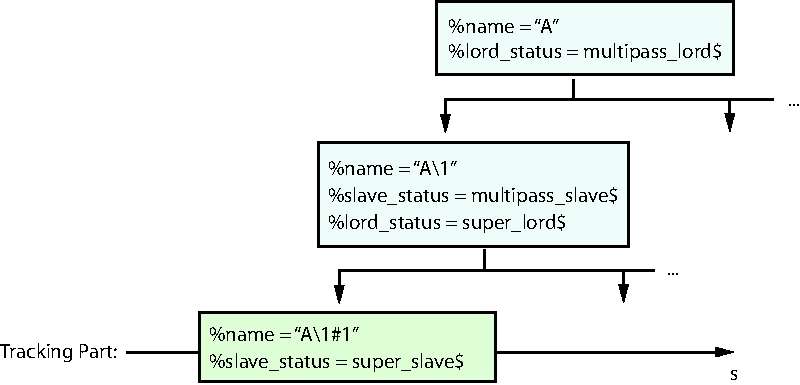
\includegraphics[width=5.5in]{superimpose-and-multipass.pdf}
\caption[Example of multipass combined with superposition]
{Example of multipass combined with superposition. A \vn{multipass_lord}
element named \vn{A} controls a set of \vn{multipass_slaves} (only one shown).
The \vn{multipass_slave} elements are also \vn{super_lord} elements and they
will control \vn{super_slave} elements in the tracking part of the branch.}
\label{f:super.mul}
\end{figure}

For lord/slave pairs,
Table~\ref{f:lord.slave.b} lists the valid combinations of
\vn{%lord_status} values in the lord element and \vn{%slave_status}
values in the slave element. Thus, for example, a
\vn{super_slave} may only be controlled by a \vn{super_lord}. In the
example in Section~\sref{s:multipass}, element \vn{A} would be a
\vn{multipass_lord} and \vn{A\B1} and \vn{A\B2} would be
\vn{multipass_slave}s. When superposition is combined with multipass,
the elements in the tracking part of the branch will be
\vn{super_slave}s.  These elements will be controlled by
\vn{super_lord}s which will also be \vn{multipass_slave}s and these
\vn{super_lord}/\vn{multipass_slave} elements will be controlled by
\vn{multipass_lord}s. This is illustrated in \fig{f:super.mul}.

\index{ele_struct!\%n_lord}\index{ele_struct!\%n_slave}
The number of slave elements that a lord controls is given by the value
of the lord's \vn{%n_slave} component. Additionally, the number of lord
elements that the slave has is given by the value of the slave's.
\vn{%n_lord} component. To find the slaves and lords of a given element,
use the routines \Hyperref{r:pointer.to.slave}{pointer_to_slave} and
\Hyperref{r:pointer.to.lord}{pointer_to_lord}. Example:
\begin{example}
  type (lat_struct), target :: lat
  type (ele_struct), pointer :: this_ele, lord_ele, slave_ele
  ...
  this_ele => lat%ele(321)    ! this_ele points to a given element in the lattice

  do i = 1, this_ele%n_lord   ! Loop over all lords of this_ele
    ! lord_ele points to the i^th lord element of this_ele
    lord_ele => pointer_to_lord (this_ele, i)  
    ...
  enddo

  do i = 1, this_ele%n_slave  ! Loop over all slaves of this_ele
    ! slave_ele points to the i^th slave element of this_ele
    slave_ele => pointer_to_slave (this_ele, i) 
    ...
  enddo
\end{example}
The lord/slave bookkeeping is bidirectional. That is, 
for any given element, call it \vn{this_ele}, consider the
i\Th lord:
\begin{example}
  lord_ele_i => pointer_to_lord (this_ele, i)
\end{example}
then there will always be some index j such that the 
element pointed to by
\begin{example}
  pointer_to_slave(lord_ele_i, j)
\end{example}
is the original element \vn{this_ele}. The same is true for
the slaves of any given element. That is, for the i\Th slave
\begin{example}
  slave_ele_i => pointer_to_slave (this_ele, i)
\end{example}
there will always be some index j such that the 
element pointed to by
\begin{example}
  pointer_to_lord(slave_ele_i, j)
\end{example}

\index{slave!ordering}\index{lords!ordering}
\index{super_lord}\index{super_slave}
\index{multipass_lord}\index{multipass_slave}
\index{patch}
The following ordering of slaves and lords is observed:
  \begin{description}
  \item[Slaves of a super_lord:] \Newline
The associated \vn{super_slave} elements of a given \vn{super_lord}
element are ordered from the entrance end of the \vn{super_lord}
to the exit end. That is, in the code snippet above,
\vn{pointer_to_slave (this_ele, 1)} will point to the slave at
the start of the \vn{super_lord} and 
\vn{ pointer_to_slave (this_ele, this_ele%n_lord)}
will point to the slave at the exit end of the \vn{super_lord}.
  \item[Slaves of a multipass_lord:] \Newline
The associated \vn{multipass_slave} elements of a 
\vn{multipass_lord} element are ordered by pass number. That is, 
in the code snippet above, \vn{pointer_to_slave (this_ele, i)}
will point to the slave of the $i$\Th pass.
  \item[Lord of a multipass_slave:] \Newline
A \vn{multipass_slave} will have exactly one associated \vn{multipass_lord}
and this lord will be the first one. That is, 
\vn{pointer_to_lord (this_ele, 1)}.
  \end{description}

\index{control_struct}
The element control information is stored in the \vn{lat%control(:)} array.
Each element of this array is a \vn{control_struct} structure 
\begin{example}
  type control_struct
    type (expression_atom_struct), allocatable :: stack(:) ! Evaluation stack
    type (lat_ele_loc_struct) slave ! Slave location
    type (lat_ele_loc_struct) lord  ! Lord location
    integer ix_attrib               ! index of controlled attribute 
  end type
\end{example}
\index{girder}\index{overlay}\index{group}
\index{lat_struct!\%control}
Each element in the \vn{lat%control(:)} array holds the information on
one lord/slave pair. The \vn{%lord} component gives the location of
the lord element which is always in the root branch --- branch 0. The
\vn{%slave} component give the element location of the slave element.
The \vn{%stack} and \vn{%ix_attrib} components are used to store the
arithmetic expression and attribute index for \vn{overlay} and \vn{group}
control. The appropriate control_struct for a given lord/slave pair
can be obtained from the optional fourth argument of the
\Hyperref{r:pointer.to.lord}{pointer_to_lord} and
\Hyperref{r:pointer.to.slave}{pointer_to_slave} functions.  Example:
The following prints a list of the slaves, along with the attributes
controlled and coefficients, on all group elements in a lattice.
\begin{example}
  type (lat_struct), target :: lat
  type (ele_struct), pointer :: lord, slave
  type (control_struct), pointer :: con
  ...
  do i = lat%n_ele_track+1, lat%n_ele_max  ! loop over all lords
    lord => lat%ele(i) 
    if (lord%lord_status = group_lord$) then 
      print *, 'Slaves for group lord: ', lord%name
      do j = 1, lord%n_slave
        slave => pointer_to_slave (lord, j, con)
        attrib_name = attribute_name (slave, con%ix_attrib)
        print *, i, slave%name, attrib_name, con%coef
      enddo
    endif
  enddo
\end{example}

\index{lat_struct!\%control}\index{lat_struct!\%n_slave_field}
\index{lat_struct!\%ix1_slave}\index{lat_struct!\%n_slave}
The elements in the \vn{lat%control(:)} array associated with
the slaves of a given lord are in the same order as the slaves and the 
index of the associated \vn{lat%control(:)} element of the first slave 
is given by the \vn{%ix1_slave} component of the lord
Example:
\begin{example}
  type (lat_struct), target :: lat
  type (ele_struct), pointer :: lord, slave
  type (control_struct), pointer :: con1, con2
  ...
  lord => lat%ele(i)                    ! Point to some lord
  do j = 1, lord%n_slave
    slave => pointer_to_slave (lord, j, con1)
    con2 => lat%control(lord%ix1_slave+j-1) ! con1 and con2 are the same.
  enddo
\end{example}

\index{ele_struct!\%ic1_lord}\index{ele_struct!\%n_lord}
\index{lat_struct!\%ic}\index{ele_struct!\%n_lord_field}
Except for a \vn{slice_slave}, the \vn{%ic1_lord}, \vn{%n_lord}, and \vn{%n_lord_field} components
of a given slave element, along with the \vn{lat%ic(:)} array, can be used to find the lords of the
slave.  Simplified, the code for the \Hyperref{r:pointer.to.lord}{pointer_to_lord} function is:
\begin{example}
  function pointer_to_lord (slave, ix_lord, con, ...) result (lord_ptr)
    implicit none
    type (lat_struct), target :: lat
    type (ele_struct) slave
    type (ele_struct), pointer :: lord_ptr
    type (control_struct), pointer, optional :: control
    integer ix_lord, icon
    !
    icon = lat%ic(slave%ic1_lord + ix_lord - 1)
    lord_ptr => lat%ele(lat%control(icon)%lord%ix_ele)
    if (present(con)) con => lat%control(icon)
  end function
\end{example}
This method for finding the lords of an element is considered
``private''. That is, no code outside of the official \bmad library
should rely on this.

\vn{slice_slave} element bookkeeping has is different depending upon
whether the element being sliced is a \vn{super_slave} or not. If the
element being sliced is a \vn{super_slave}, a \vn{slice_slave} element
that is created is, for bookkeeping purposes, considered to be a slave
of the \vn{super_slave}'s lords. In this case, the bookkeeping is
exactly the same as that of any \vn{super_slave}, and
\vn{pointer_to_lord} will return a pointer to one of the
\vn{super_slave}'s lords.

On the other hand, if a non \vn{super_slave} element is being sliced,
the \vn{%lord} pointer component of the \vn{slice_slave} will be set to
point to the element being sliced.

%----------------------------------------------------------------------------
\section{Lattice Bookkeeping}
\label{s:lat.bookkeeping}

\index{reference energy}
The term ``lattice bookkeeping'' refers to the updating of
the appropriate parameter values when a given parameter in the lattice is
changed. For example, if the accelerating gradient of an \vn{lcavity}
element is modified, the reference energy parameter of all elements
downstream of the \vn{lcavity} will need to be changed and this can
also alter the transfer maps of the \vn{lcavity} and downstream
elements. \bmad divides the lattice bookkeeping into ``core'' part
and everything else. The core part itself is divided into five parts:
  \begin{description}
  \item[Attribute bookkeeping] \Newline
This refers to intra-element dependent attribute bookkeeping (\sref{s:depend}).
  \item[Control bookkeeping] \Newline
This refers to Lord/Slave bookkeeping for \vn{overlay}
(\sref{s:overlay}) and \vn{group} (\sref{s:group})elements, and for
\vn{superposition} (\sref{s:super}) and \vn{multipass}
(\sref{s:multipass}) lords.
  \item[Floor Position bookkeeping]
This refers to bookkeeping to keep track of an elements global ``floor'' position
stored in the \vn{ele%floor} structure.
  \item[Length bookkeeping]
This refers to bookkeeping to keep track of the longitudinal s-position of an element
stored in the \vn{ele%s} component.
  \item[Reference Energy bookkeeping]
This refers to the reference energy assigned to each element (\sref{s:ref.energy.prog}).
\vn{ele%value(E_tot\$)} and \vn{ele%value(p0c\$)}
  \end{description}

\index{bookkeeping!automatic}
\index{bookkeeping!intelligent}
Historically, as the concept of lattice bookkeeping was being
developed, to be back compatible with existing programs, calls to
bookkeeping routines were added to calculational routines such as the
tracking routine \Hyperref{r:track1}{track1} and the routine for
calculating the linear transfer map \Hyperref{r:make.mat6}{make_mat6}.
This ``automatic'' bookkeeping system is inefficient since there is no
good way to keep track of what element attributes have been modified
which leads to redundant bookkeeping calculations. Eventually, as
\bmad developed and became more complicated, it was found that the
unnecessary bookkeeping load was generally causing a significant
slowdown in program execution time --- even in programs where no
element attributes were changed. To avoid this, an ``intelligent''
bookkeeping system was developed. In order to be back compatible with
existing programs, the automatic bookkeeping system is the
default. However, given the fact that the automatic bookkeeping system
has known deficiencies, and given the overhead with maintaining two
bookkeeping systems, the current plan is to start phasing out the
automatic bookkeeping system sometime in the not-so-far future. Thus
old programs should be converted to the new system and all new
programs should use the new bookkeeping system.

\index{bmad_common_struct!auto_bookkeeper}
To use intelligent bookkeeping, a program must set the global
\vn{bmad_com%auto_bookkeepper} to false. This is done once at the
start of the program. When a set of attributes needs to be modified,
the
\Hyperref{r:set.flags.for.changed.attribute}{set_flags_for_changed_attribute}
routine must be called for each element attribute that is set. After
all the attributes have been set,
\Hyperref{r:lattice.bookkeeper}{lattice_bookkeeper} is called to do
the core bookkeeping. Example
\begin{example}
  type (lat_struct) lat
  ...
  bmad_com%auto_bookkeeper = .false.    ! Only needs to be done once.
  ...
  lat%ele(i)%value(gradient$) = 1.05e6  ! Change, say, the gradient of an RFCavity
  call set_flags_for_changed_attribute (lat%ele(i), lat%ele(i)%value(gradient$))

  ... Set attributes of other elements ...

  call lattice_bookkeeper (lat)         ! Do once after all attribute sets done.
\end{example}
The argument list for \vn{set_flags_for_changed_attribute} is 
\begin{example}
  set_flags_for_changed_attribute (ele, attribute)
\end{example}
The \vn{attribute} argument may be either real, integer, or logical.

\index{ele!\%status}
\index{bookkeeper_status_struct}
The \vn{set_flags_for_changed_attribute} routine sets flags in the
\vn{ele%status} structure. This structure is of type
\vn{bookkeeper_status_struct} and looks like
\begin{example}
  type bookkeeper_status_struct
    integer attributes      ! Intra element dependent attribute status
    integer control         ! Lord/slave bookkeeping status
    integer floor_position  ! Global (floor) geometry status
    integer length          ! Longitudinal position status
    integer ref_energy      ! Reference energy status
    integer mat6            ! Linear transfer map status
    integer rad_int         ! Radiation integrals cache status
  end type
\end{example}
All components of this structure give the status of some lattice
bookkeeping aspect. The first five components of this structure
correspond to the five core bookkeeping parts discussed above. The
other two components are discussed below.

Possible values for the status components are
\begin{example}
  super_ok\$
  ok\$
  stale\$
\end{example}
The \vn{set_flags_for_changed_attribute} routine sets the appropriate
status components of an element to \vn{stale\$} which marks that
element for the appropriate bookkeeping. When the bookkeeping is done
by \vn{lattice_bookkeeper}, the \vn{stale\$} status components are set
to \vn{ok\$}. The \vn{super_ok\$} value is reserved for use by any
program that needs to do its own custom bookkeeping. How this works is
as follows: The \bmad bookkeeping routines will never convert a status
component with value \vn{super_ok\$} to \vn{ok\$} without first doing
some needed bookkeeping. Thus if a program sets a status component to
\vn{super_ok\$} and then later on finds that the status component is
set to \vn{ok\$}, the program knows that bookkeeping has been done. An
example will make this clear. Suppose a program needs to keep track of
a collection of high order transfer maps between various points in a
lattice. Suppose that the constant calculation of these maps would
slow the program done so it is desired to recalculate a given map only
when necessary. To implement this, the program could set the
\vn{ele%status%mat6} attribute of all the element to \vn{super_ok\$}
when the maps are calculated. If the program subsequently finds a
\vn{ele%status%mat6} attribute of an element set to \vn{ok\$} it knows
that it should recalculate any transfer maps that span that element.

It is guaranteed that when \vn{lattice_bookkeeper} is run,
all five core status components will not be \vn{stale\$}.
The routines used by \vn{lattice_bookkeeper} are:
\begin{example}
  \Hyperref{r:attribute.bookkeeper}{attribute_bookkeeper}      ! Intra-element attributes
  \Hyperref{r:control.bookkeeper}{control_bookkeeper}        ! Lord/slave control
  \Hyperref{r:s.calc}{s_calc}                    ! Longitudinal element s-position
  \Hyperref{r:lat.geometry}{lat_geometry}              ! Global (floor) positions.
  \Hyperref{r:lat.compute.ref.energy.and.time}{lat_compute_ref_energy_and_time}  ! Reference energy 
\end{example}
In general, these routines should not be called directly since the
correct way to do things is not always straight forward. See the code
for \vn{lattice_bookkeeper} for more details.

After the core bookkeeping is done, a program can call
\Hyperref{r:lat.make.mat6}{lat_make_mat6} to remake the transfer matrices.
\vn{lat_make_mat6} will remake the transfer matrices if either the
\vn{ele%status%mat6} flag is \vn{stale\$} or the reference orbit
around which the existing transfer matrix was computed has shifted.
\vn{lat_make_mat6} will set the \vn{ele%status%mat6} flag to \vn{ok\$}
for all elements whose transfer matrices are recomputed.

%----------------------------------------------------------------------------
\section{Beam_start Component}
\label{s:lat.beam.start}

\index{beam_start}
\index{lat_struct!\%beam_start}
The \vn{lat%beam_start} component is a \vn{coord_struct} structure for
holding the information obtained from \vn{beam_start} statements
(\sref{s:beam.start}) in a \bmad lattice file.

This component is not used in any standard \bmad calculation. It is up
to an individual program to use as desired.


\chapter{Lattice Element Manipulation}
\label{c:ele.manip}

%--------------------------------------------------------------------------
\section{Creating Element Slices}
\label{s:ele.slice}

\index{sbend}\index{rbend}\index{wiggler}
It is sometimes convenient to split an element longitudinally into
``slices'' that represent a part of the element.  This is complicated
by the fact that elements are not necessarily uniform.  For example,
map type wigglers are nonuniform and bend elements have end effects.
Furthermore, attributes like \vn{hkick} need to be scaled with the
element length.

To create an element slice, the routine
\Hyperref{r:create.element.slice}{create_element_slice} can be used.
Example:
\begin{example}
  type (ele_struct) ele, sliced_ele
  ...
  sliced_ele = ele
  sliced_ele%value(l$) = l_slice ! Set the sliced element's length
  call create_element_slice (sliced_ele, ele, l_start, param, ...)
\end{example}
See the documentation on \vn{create_element_slice} for more details (\sref{s:getf}).

%----------------------------------------------------------------------------
\section{Adding and Deleting Elements From a Lattice}
\label{s:lat.add.delete}

Modifying the number of elements in a lattice involves a bit of
bookkeeping. To help with this there are a number of routines. 

The routine \Hyperref{r:remove.eles.from.lat}{remove_eles_from_lat} is
used to delete elements from a lattice.

For adding elements there are three basic routines: To add a lord
element, the \Hyperref{r:new.control}{new_control} routine is used.
To add a new element to the tracking part of the lattice, use the
\Hyperref{r:insert.element}{insert_element} routine. Finally, to split
an element into two pieces, the routine
\Hyperref{r:split.lat}{split_lat} is used. These basic routines are
then used in such routines as
\Hyperref{r:create.overlay}{create_overlay} that creates overlay
elements, \Hyperref{r:create.group}{create_group} which creates group
elements, \Hyperref{r:add.superimpose}{add_superimpose} which
superimposes elements, etc. Example:
\begin{example}
  type (lat_struct), target :: lat
  type (ele_struct), pointer :: g_lord, slave

  type (control_struct) con(1)
  integer ix, n
  logical err_flag
  ...
  call new_control (lat, ix)
  g_lord => lat%ele(ix)
  allocate (ele%control_var(1))
  ele%control_var(1)%name = 'A'
  call reallocate_expression_stack(con(1)%stack, 10))
  call expression_string_to_stack ('3.2*A^2', con(1)%stack, n, err_flag)
  con(1)%ix_attrib = k1$
  call lat_ele_locator ('Q1W', lat, eles)
  con(1)%slave = ele_to_lat_loc(eles(1)%ele)
  call create_group (g_lord, con, err_flag)
\end{example}
This example constructs a group element with one variable with name
\vn{A} controlling the \vn{K1} attribute of element \vn{Q1W} using the
expression ``$3.2 \cdot A^2$'' where \vn{A} is the name of the control
variable.

For constructing \vn{group} elements (but not \vn{overlay} elements),
the controlled attribute (set by \vn{con(1)%ix_attrib} in the above
example) can be set to, besides the set of element attributes, any one
in the following list:
\begin{example}
  accordion_edge$  ! Element grows or shrinks symmetrically
  start_edge$      ! Varies element's upstream edge s-position
  end_edge$        ! Varies element's downstream edge s-position
  s_position$      ! Varies element's overall s-position. Constant length.
\end{example}
See Section~\sref{s:group} for the meaning of these attributes

%---------------------------------------------------------------------------
\section{Finding Elements and Changing Attribute Values}
\label{s:lat.ele.change}

\index{ele_struct!\%ix_ele}
The routine \Hyperref{r:lat.ele.locator}{lat_ele_locator} 
can be used to search for an element
in a lattice by name or key type or a combination of both. Example:
\begin{example}
  type (lat_struct) lat
  type (ele_pointer_struct), allocatable :: eles(:)
  integer n_loc; logical err
  ...
  call lat_ele_locator ("quad::skew*", lat, eles, n_loc, err)
  print *, 'Quadrupole elements whose name begins with the string "SKEW":'
  print *, 'Name                 Branch_index        Element_index'
  do i = 1, n_loc  ! Loop over all elements found to match the search string.
    print *, eles(i)%ele%name, eles(i)%ele%ix_branch, eles(i)%ele%ix_ele
  enddo
\end{example}
This example finds all elements where \vn{ele%key} is \vn{quadrupole\$} 
and \vn{ele%name} starts with ``\vn{skew}''. See the documentation on 
\vn{lat_ele_locator} for more details on the syntax of the search string.

The \vn{ele_pointer_struct} array returned by \vn{lat_ele_locator} is
an array of pointers to \vn{ele_struct} elements
\begin{example}
  type ele_pointer_struct
    type (ele_struct), pointer :: ele
  end type
\end{example}
The \vn{n_loc} argument is the number of elements found and the \vn{err} argument
is set True on a decode error of the search string.

Once an element (or elements) is identified in the lattice,
it's attributes can be altered. However, care must be taken that an element's attribute
can be modified (\sref{s:depend}). The function \vn{attribute_free} will
check if an attribute is free to vary.
\begin{example}
  type (lat_struct) lat
  integer ix_ele
  ...
  call lat_ele_locator ('Q10W', lat, eles, n_loc, err)   ! look for an element 'Q10W'
  free = attribute_free (eles(i)%ele, 'K1', lat, .false.)
  if (.not. free) print *, 'Cannot vary k1 attribute of element Q10W'
\end{example}

With user input the routine \vn{pointer_to_attribute} is a convenient
way to obtain from an input string a pointer that points to the
appropriate attribute. For example:
\begin{example}
  type (lat_struct) lat
  type (ele_pointer_struct), allocatable :: eles(:)
  type (all_pointer_struct) attrib_ptr
  character(40) attrib_name, ele_name
  real(rp) set_value
  logical err
  integer ie
  ...
  write (*, '(a)', advance = 'no') ' Name of element to vary: '
  accept '(a)', ele_name
  write (*, '(a)', advance = 'no') ' Name of attribute to vary: '
  accept '(a)', attrib_name
  write (*, '(a)', advance = 'no') ' Value to set attribute at: '
  accept *, set_value

  call lat_ele_locator (name, lat, eles, n_loc, err)
  if (err) ....
  do ie = 1, size(eles)
    call pointer_to_attribute (eles(ie)%ele, attrib_name, .false., attrib_ptr, err)
    if (err) exit      ! Do nothing on an error
    if (associated(attrib_ptr%r)) then  ! Real attribute
      attrib_ptr%r = set_value  ! Set the attribute
    elseif (associated(attrib_ptr%i)) then ! Integer attribute
      attrib_ptr%i = nint(set_value)
    else
      print *, 'Not a real or integer type attribute!'
    endif
  enddo

  call lattice_bookkeeper (lat)  ! Bookkeeping needed due to parameter change 
\end{example}

changing an element attribute generally involves changing values in the 
\vn{%ele(i)%value(:)} array. This is done using the 
\Hyperref{r:set.ele.attribute}{set_ele_attribute} routine. For example:
\begin{example}
  type (lat_struct) lat
  type (ele_pointer_struct), allocatable :: eles(:)
  integer n_loc, n
  logical err_flag, make_xfer_mat
  ...
  call lat_ele_locator ('Q01W', lat, eles, n_loc, err_flag)
  do n = 1, n_loc
    call set_ele_attribute (eles(n)%ele, 'K1 = 0.1', lat, err_flag)
  enddo
\end{example}
\index{overlay}
This example sets the \vn{K1} attribute of all elements named \vn{Q01W}.
\vn{set_ele_attribute} checks whether an element is actually free to
be varied and sets the \vn{err_flag} logical accordingly. An element's
attribute may not be freely varied if, for example, the attribute is
controlled via an \vn{Overlay}.




\chapter{Reading and Writing Lattices}

%----------------------------------------------------------------------------
\section{Reading in Lattices}
\label{s:lat.readin}
\index{lattice files!reading}

\index{XSIF}\Hyperref{r:xsif.parser}{xsif_parser}
\Hyperref{r:bmad.parser}{bmad_parser}\Hyperref{r:bmad.parser2}{bmad_parser2}

\bmad has routines for reading XSIF (\sref{s:lattice.file.formats}) and
\bmad formatted lattice files. The subroutine to read in an XSIF lattice
file is \Hyperref{r:xsif.parser}{xsif_parser}. There are two subroutines in \bmad to read
in a \bmad standard lattice file: \Hyperref{r:bmad.parser}{bmad_parser} and
\Hyperref{r:bmad.parser2}{bmad_parser2}. \vn{bmad_parser} is used to initialize a
\vn{lat_struct} (\sref{c:lat.struct}) 
structure from scratch using the information from a
lattice file. Unless told otherwise, after reading in the lattice,
\vn{bmad_parser} will compute the 6x6 transfer matrices for each element
and this information will be stored in the \vn{digested file}
(\sref{s:digested}) that is created.  Notice that \vn{bmad_parser}
does {\em not} compute any Twiss parameters.

\Hyperref{r:bmad.parser2}{bmad_parser2} is typically used after \vn{bmad_parser} if there is
additional information that needs to be added to the lattice. For
example, consider the case where the aperture limits for the elements 
is stored in a file that is separate from the main lattice definition
file and it is undesireable to put a \vn{call} statement in one file
to reference the other.
To read in the lattice information along with the aperture limits, 
there are two possibilities: One possibility 
is to create a third file that calls the first two:
\begin{verbatim}
 ! This is a file to be called by bmad_parser
 call, file = 'lattice_file'
 call, file = 'aperture_file'
\end{verbatim}
and then just use \vn{bmad_parser} to parse this third file. The
alternative is to use \vn{bmad_parser2} so that the program code looks
like:
\begin{verbatim}
  ! program code to read in everything
  type (lat_struct) lat
  call bmad_parser ('lattice_file', lat)       ! read in a lattice.
  call bmad_parser2 ('aperture_file', lat)     ! read in the aperture limits.
\end{verbatim}

An alternative to using \vn{bmad_parser} and \vn{xsif_parser} is to
use the combined \bmad and XSIF parser
\Hyperref{r:bmad.and.xsif.parser}{bmad_and_xsif_parser}. This parser
will assume that the input file is using \bmad syntax unless the file
name is prefixed by the string \vn{``xsif::''}.

%----------------------------------------------------------------------------
\section{Digested Files}
\index{digested files}

\index{bmad_parser}
\index{bmad version number}
Since parsing can be slow, once the \vn{bmad_parser} routine
has transfered the
information from a lattice file into the \vn{lat_struct} it will make
what is called a digested file. A digested file is an image of the
\vn{lat_struct} in binary form. When \vn{bmad_parser} is called, 
it first looks in the same directory as the lattice
file for a digested file whose name is of the form:
\begin{verbatim}
  'digested_' // LAT_FILE 
\end{verbatim}
where \vn{LAT_FILE} is the lattice file name. If \vn{bmad_parser} finds the digested
file, it checks that the file is not out--of--date (that is, whether the
lattice file(s) have been modified after the digested file is made).
\vn{bmad_parser} can do this since the digested file contains the names
and the dates of all the lattice files that were involved. Also stored
in the digested file is the ``\bmad \vn{version number}''. The \bmad
version number is a global parameter that is increased (not too
frequently) each time a code change involves modifying the structure of
the \vn{lat_struct} or \vn{ele_struct}. If the \bmad version number in
the digested file does not agree with the number current when \vn{bmad_parser}
was compiled, or if the digested
file is out--of--date, a warning will be printed, and \vn{bmad_parser}
will reparse the lattice and create a new digested file.

\index{taylor map!with digested files}
Since computing Taylor Maps can be very time intensive,
\vn{bmad_parser} tries to reuse Taylor Maps it finds in the digested
file even if the digested file is out--of--date. To
make sure that everything is OK, \vn{bmad_parser} will check that the attribute
values of an element needing a Taylor map are the same as the
attribute values of a corresponding element in the digested file
before it reuses the map. Element names are not a factor in this
decision.

This leads to the following trick: If you want to read in a lattice
where there is no corresponding digested file, and if there is another
digested file that has elements with the correct Taylor Maps, then, to
save on the map computation time, simply make a copy of the digested
file with the digested file name corresponding to the first lattice.

\Hyperref{r:read.digested.bmad.file}{read_digested_bmad_file}
\Hyperref{r:write.digested.bmad.file}{write_digested_bmad_file}
The digested file is in binary format and is not human readable but it
can provide a convenient mechanism for transporting lattices between
programs. For example, say you have read in a lattice, changed
some parameters in the \vn{lat_struct}, and now you want to do some
analysis on this modified \vn{lat_struct} using a different program. 
One possibility is to have the first program create a digested file
\begin{example}
  call write_digested_bmad_file ('digested_file_of_mine', lat)
\end{example}
and then read the digested file in with the second program
\begin{example}
  call read_digested_bmad_file ('digested_file_of_mine', lat)
\end{example}
An alternative to writing a digested file is to write a lattice file
using \vn{write_bmad_lattice_file}

%----------------------------------------------------------------------------
\section{Writing Lattice files}
\label{s:lat.write}
\index{lattice files!MAD files}
\index{MAD}

\Hyperref{r:write.bmad.lattice.file}{write_bmad_lattice_file}
To create a \bmad lattice file from a \vn{lat_struct} instance, use the routine
\Hyperref{r:write.bmad.lattice.file}{write_bmad_lattice_file}.
\index{MAD!MAD-8}
\mad--8, \mad--X, or \vn{XSIF} compatible lattice 
files can be created from a \vn{lat_struct} variable 
using the routine 
\Hyperref{r:write.lattice.in.foreign.format}{write_lattice_in_foreign_format}:
\begin{example}
  type (lat_struct) lat             ! lattice
  ...
  call bmad_parser (bmad_lat_file, lat)               ! Read in a lattice
  call write_lattice_in_foreign_format ('lat.mad', 'MAD-8', lat)  ! create MAD file
\end{example}
Information can be lost when creating a \mad or \vn{XSIF} file.
For example, neither \mad nor \vn{XSIF} has the concept of 
things such as \vn{overlay}s and \vn{group}s.


\chapter{Normal Modes: Twiss Parameters, Coupling, Emittances, Etc.}
\label{c:normal.modes}

%-----------------------------------------------------------------------------
\section{Components in the Ele\_struct}
\label{s:twiss.ele}

\index{ele_struct!\%gamma_c}
\index{ele_struct!\%c_mat}
\index{ele_struct!\%a}\index{ele_struct!\%b}\index{ele_struct!\%z}
The \vn{ele_struct} (\sref{c:ele.struct}) has a number of components that
hold information on the Twiss parameters, dispersion, and coupling
at the exit end of the element. The Twiss parameters of the three 
normal modes (\sref{s:coupling})
are contained in the \vn{ele%a}, \vn{ele%b}, and \vn{ele%z} 
components which are of type \vn{twiss_struct}:
\index{twiss_struct}
\begin{example}
  type twiss_struct
    real(rp) beta         ! Twiss Beta function
    real(rp) alpha        ! Twiss Alpha function
    real(rp) gamma        ! Twiss gamma function
    real(rp) phi          ! Normal mode Phase advance
    real(rp) eta          ! Normal mode dispersion
    real(rp) etap         ! Normal mode dispersion derivative
    real(rp) sigma        ! Normal mode beam size
    real(rp) sigma_p      ! Normal mode beam size derivative
    real(rp) emit         ! Geometric emittance
    real(rp) norm_emit    ! Energy normalized emittance (= \(\gamma \, \epsilon\))
  end type 
\end{example}
\index{xy_disp_struct}
The projected horizontal and vertical dispersions in an
\vn{ele_struct} are contained in the \vn{ele%x} and \vn{ele%y}
components. These components are of type \vn{xy_disp_struct}:
\index{xy_disp_struct}
\begin{example}
  type xy_disp_struct
    real(rp) eta     ! Projected dispersion 
    real(rp) etap    ! Projected dispersion derivative.
  end type 
\end{example}

\index{ele_struct!\%emit}\index{ele_struct!\%norm_emit}
\index{ele_struct!\%sigma}\index{ele_struct!\%sigma_p}
The components \vn{ele%emit}, \vn{ele%norm_emit}, \vn{ele%sigma},
\vn{ele%sigma_p} are not set by the standard \bmad routines and are
present for use by any program.

\index{ele_struct!\%c}\index{ele_struct!\%gamma_c}
The relationship between the projected and normal mode dispersions are
given by \Eq{avx}. The 2x2 coupling matrix $\bfC$ (\Eq{vgicc1}) is
stored in the \vn{ele%c_mat(2,2)} component of the \vn{ele_struct} and the
$\gamma$ factor of \Eq{vgicc1} is stored in the \vn{ele%gamma_c}
component. There are several routines to manipulate the coupling
factors. For example:
\begin{example}
  \Hyperref{r:c.to.cbar}{c_to_cbar}(ele, cbar_mat)             ! Form Cbar(2,2) matrix
  \Hyperref{r:make.v.mats}{make_v_mats}(ele, v_mat, v_inv_mat)   ! Form V coupling matrices.
\end{example}
See \sref{r:mat} for a complete listing of such routines.

Since the normal mode and projected dispersions are related, when one
is changed within a program the appropriate change must be made to the
other. To make sure everything is consistent, the
\Hyperref{r:set.flags.for.changed.attribute}{set_flags_for_changed_attribute}
routine can be used. Example:
\begin{example}
  type (lat_struct), target :: lat
  real(rp), pointer :: attrib_ptr
  ...
  attrib_ptr => lat%ele(ix_ele)%value(k1$) ! Point to some attribute.
  attrib_ptr = value                       ! Change the value.
  call set_flags_for_changed_attribute (lat%ele(ix_ele), attrib_ptr)
\end{example}

The \vn{%mode_flip} logical component of an \vn{ele_struct} indicates
whether the $a$ and $b$ normal modes have been flipped relative to the
beginning of the lattice. See Sagan and Rubin\cite{b:coupling} for a
discussion of this. The convention adopted by \bmad is that the
\vn{%a} component of all the elements in a lattice will all correspond
to the same physical normal mode. Similarly, the \vn{%b} component of
all the elements will all correspond to some (other) physical normal
mode.  That is, at an element where there is a mode flip (with
\vn{%mode_flip} set to True), the \vn{%a} component actually
corresponds to the $\bfB$ matrix element in \Eq{ua00b} and vice
versa. The advantage of this convention is that calculations of mode
properties (for example the emittance), can ignore whether the modes
are flipped or not.

The normal mode analysis of Sagan and Rubin, while it has the benefit
of simplicity, is strictly only applicable to lattices where the RF
cavities are turned off.  The full 6-dimensional analysis is
summarized by Wolski\cite{b:wolski.coupling}.  The
\Hyperref{r:normal.mode3.calc}{normal_mode3_calc} routine perform the
full analysis. The results are put in the \vn{%mode3} component of the
\vn{ele_struct} which is of type \vn{mode3_struct}:
\index{ele_struct!\%mode3}
\index{mode3_struct}
\begin{example}
  type mode3_struct
    real(rp) v(6,6)
    type (twiss_struct) a, b, c
    type (twiss_struct) x, y
  end type
\end{example}
The 6-dimensional \vn{mode3%v(6,6)} component is the analog of the 4-dimensional
$\bfV$ matrix appearing in \Eq{tvuv}.

%-----------------------------------------------------------------------------
\section{Tune and Twiss Parameter Calculations}
\label{s:twiss}
\index{twiss parameters}
\index{twiss parameters!calculation}
\index{tune!calculation}

A calculation of the Twiss parameters starts with the Twiss parameters
at the beginning of the lattice. For linear machines, these Twiss parameters
are generally set in the input lattice file (\sref{s:beginning}). For
circular machines, 
the routine \Hyperref{r:twiss.at.start}{twiss_at_start} 
may be used (\sref{s:beginning})
\begin{example}
  type (lat_struct) lat
  ...
  if (lat%param%geometry == closed$) call twiss_at_start(lat)
\end{example}
In either case, the initial Twiss parameters are placed in \vn{lat%ele(0)}. 
The tune is placed in the variables \vn{lat%a%tune} and \vn{lat%b%tune}.

To propagate the Twiss, coupling and dispersion parameters from the
start of the lattice to the end, the routine,
\Hyperref{r:twiss.propagate.all}{twiss_propagate_all} can be
used. This routine works by repeated calls to
\Hyperref{r:twiss.propagate1}{twiss_propagate1} which does a single
propagation from one element to another. The Twiss propagation depends
upon the transfer matrices having already computed
(\sref{c:tracking}).  \vn{twiss_propagate_all} also computes the Twiss
parameters for all the lattice branches. 

Before any Twiss parameters can be calculated, the transfer matrices
stored in the lattice elements must be computed. 
\Hyperref{r:bmad.parser}{bmad_parser} does
this automatically about the zero orbit. If, to see nonlinear effects,
a different orbit needs to be used for the reference, The routine
\Hyperref{r:twiss.and.track}{twiss_and_track} can be used. For example:
\begin{example}
  type (lat_struct) lat
  type (coord_struct), allocatable :: orbit(:)
  call bmad_parser ('my_lattice', lat)
  call twiss_and_track (lat, orb, ok)
\end{example}

Once the starting Twiss parameters are set,
\Hyperref{r:twiss.propagate.all}{twiss_propagate_all} can be used to
propagate the Twiss parameters to the rest of the elements
\begin{example}
\end{example}

The routine \Hyperref{r:twiss.and.track.at.s}{twiss_and_track_at_s}
can be used to calculate the Twiss parameters at any given
longitudinal location. Alternatively, to propagate the Twiss
parameters partially through a given element use the the routine
\Hyperref{r:twiss.and.track.intra.ele}{twiss_and_track_intra_ele}.

%-----------------------------------------------------------------------------
\section{Tune Setting}
\label{s:tune.set}
\index{tune!setting}

The routine \Hyperref{r:set.tune}{set_tune} can be used
to set the transverse tunes:
\begin{example}
  set_tune (phi_a_set, phi_b_set, dk1, lat, orb_, ok)
\end{example}
\vn{set_tune} varies quadrupole strengths until the desired tunes are
achieved. As input,\vn{set_tune} takes an argument \vn{dk1(:)} which is an array
that specifies the relative change to be make to the quadrupoles in the lattice.

To set the longitudinal (synchrotron) tune, the routine
\Hyperref{r:set.z.tune}{set_z_tune} can be used. 
\Hyperref{r:set.z.tune}{set_z_tune} works by varying rf cavity
voltages until the desired tune is achieved.

%-----------------------------------------------------------------------------
\section{Emittances \& Radiation Integrals}
\label{s:emit}

See Section~\sref{s:synch.ints} for details on the radiation integral
formulas.

The routine \Hyperref{r:radiation.integrals}{radiation_integrals} is used to calculate the 
normal mode emittances along with the radiation integrals:
\begin{example}
  type (lat_struct) lat
  type (normal_modes_struct) modes
  type (rad_int_all_ele_struct) ele_rad_int
  ...
  call radiation_integrals (lat, orbit, modes, rad_int_by_ele = ele_rad_int)
\end{example}
The \vn{modes} argument, which is of type \vn{normal_modes_struct},
holds the radiation integrals integrated over the entire lattice.
\begin{example}
  type normal_modes_struct
    real(rp) synch_int(0:3) ! Synchrotron integrals I0, I1, I2, and I3
    real(rp) sigE_E         ! SigmaE/E
    real(rp) sig_z          ! Sigma_Z
    real(rp) e_loss         ! Energy loss / turn (eV)
    real(rp) rf_voltage     ! Total rfcavity voltage (eV)
    real(rp) pz_aperture    ! pz aperture limit
    type (anormal_mode_struct)  a, b, z
    type (linac_normal_mode_struct) lin
  end type
\end{example}
In particular, the \vn{%a}, \vn{%b}, and \vn{%z} components, which are
of type \vn{anormal_mode_struct} hold the emittance values:
\begin{example}
  type anormal_mode_struct
    real(rp) emittance        ! Beam emittance
    real(rp) synch_int(4:6)   ! Synchrotron integrals
    real(rp) j_damp           ! damping partition number
    real(rp) alpha_damp       ! damping per turn
    real(rp) chrom            ! Chromaticity
    real(rp) tune             ! "Fractional" tune in radians
  end type
\end{example}

The \vn{ele_rad_int} argument, which is is of type
\vn{rad_int_all_ele_struct}, holds the radiation integrals on an
element-by-element basis.
\begin{example}
  type rad_int_all_ele_struct
    type (rad_int1_struct), allocatable :: ele(:) ! Array is indexed from 0
  end type
\end{example}

%-----------------------------------------------------------------------------
\section{Chromaticity Calculation}
\label{s:chrom}

\index{chromaticity}
For a circular lattice, \Hyperref{r:chrom.calc}{chrom_calc} 
calculates the chromaticity by calculating
the tune change with change in beam energy.

\Hyperref{r:chrom.tune}{chrom_tune} sets the chromaticity by 
varying the sextupoles. This is a 
very simple routine that simply divides the sextupoles into two families
based upon the local beta functions at the sextupoles.




\chapter{Tracking and Transfer Maps}
\label{c:tracking}
\index{tracking}

\index{macroparticles!tracking}
\index{tracking!Macroparticles}
\bmad has routines for tracking two types of objects called
``\vn{particles}'' and ``\vn{macroparticles}''. \vn{Particles} are
characterized by a six-vector representing the particle's phase space
coordinates and a pair of complex numbers characterizing the
particle's spin.  A macroparticle is like a particle with the
addition of a $6\times 6$ ``sigma'' matrix characterizing the size of
the macroparticle.

Macroparticle tracking was implemented in \bmad in order to simulate
particle bunches.  The idea was that far fewer macroparticles than
particles would be needed to characterize a bunch. In practice, it was
found that the complexity of handling the macroparticle sigma matrix
more than offset the reduction in the number of particles
needed. Hence, while the basic macroparticle tracking routines still
exist, macroparticle tracking is not currently maintained and the use
of this code is discouraged. However macroparticle tracking could be
revived in the future if there is a demonstrated need for it.

\index{beam}\index{bunch}
Particle tracking can be divided into ``single particle'' tracking and
``beam'' tracking. Single particle tracking is simply tracking a
single particle. Beam tracking is tracking an ensemble of particles
divided up into a number of bunches that make up a ``beam''. Both
types particle tracking are covered in this chapter.

%----------------------------------------------------------------
\section{The coord_struct}
\label{s:coord.struct}
\index{coord_struct}

\index{spin}
\index{phase space coordinates}
The \vn{coord_struct} holds the coordinates of a particle at a given
longitudinal position in the lattice. The definition of the
\vn{coord_struct} is
\begin{example}
  type coord_struct
    real(rp) vec(6)     ! (x, px, y, py, z, pz)
    real(rp) s          ! Longitudinal position.
    real(rp) t          ! Absolute time (not relative to reference).
    real(rp) spin(3)    ! (x, y, z) Spin vector
    real(rp) field(2)   ! Photon (x, y) field intensity.
    real(rp) phase(2)   ! Photon (x, y) phase.
    real(rp) charge     ! charge in a particle (Coul).
    real(rp) path_len   ! path length (used by coherent photons).
    real(rp) p0c        ! For non-photons: Reference momentum. Negative -> going backwards.
                        !     For photons: Photon momentum (not reference).
    real(rp) beta       ! Velocity / c_light. 
    integer ix_ele      ! Index of element particle was tracked through.
                        !   May be -1 or -2 if element is not associated with a lattice.
    integer ix_user     ! Not used by \bmad
    integer state       ! alive\$, lost\$, lost_neg_x_aperture\$, etc.
    integer direction   ! Longitudinal direction of motion = +/- 1
    integer species     ! Positron\$, proton\$, etc.
    integer location    ! upstream_end\$, inside\$, or downstream_end\$
end type
\end{example}

The components of the \vn{coord_struct}:
\begin{description}
\item{\%beta} \Newline
The normalized velocity $v/c$ is stored in \vn{%beta}.

\item{\%direction} \Newline
Longitudinal direction of travel. A setting of +1 is in the forward (downstream) direction and a
setting of -1 is in the reverse (upstream) direction (\sref{s:ref.construct}).  Notice that the
setting of \vn{direction} is independent of the orientation of the lattice element the particle is
traveling through. That is, for an element with reversed \vn{orientation} (\vn{ele%orientation} =
-1), a particle with \vn{direction} = 1 will be traveling towards the \vn{entrance} end of the
element and with \vn{direction} = -1 the particle will be traveling towards the \vn{exit} end
(\sref{s:ref.construct}).

\item{\%field_x, \%field_y} \Newline
The \vn{%field_x} and \vn{%field_y} components are for photon
tracking and are in units of field/sqrt(cross-section-area). That is,
the square of these units is an intensity. It is up to individual
programs to define an overall scaling factor for the intensity if
desired.

\item{\%ix_ele} \Newline
The \vn{%ix_ele} component gives the index of the element in the
\vn{lat%branch(ib)%ele(:)} array that was tracked through. If the
element tracked through is not associated with a lattice, \vn{%ix_ele}
is set to -1. When initializing a \vn{coord_struct} (see below),
\vn{%ix_ele} will be initialized to \vn{not_set\$}.

\item{\%ix_user} \Newline
The \vn{%ix_user} component is for use by code outside of the \bmad library.
\bmad does not use this component.

\item{\%location} \Newline
The \vn{%location} component indicates where a particle is
longitudinally with respect to the element being
tracked. \vn{%location} will be on of:
\begin{example}
  entrance_end\$
  inside\$
  exit_end\$
\end{example}
\vn{entrance_end\$} indicates that the particle is at the element's
entrance ($-s$) end and \vn{exit_end\$} indicates that the particle is
at the element's exit ($+s$) end.  \vn{inside\$} indicates that the
particle is in between. If the element has edge fields (for example,
the \vn{e1} and \vn{e2} edge fields of a bend), a particle at the
\vn{entrance_end\$} or \vn{exit_end\$} is considered to be just
outside the element.

\item{\%p0c} \Newline
For charged-particles, the reference momentum in eV is stored in the
\vn{%p0c} component. For photons, \vn{%p0c} is the actual (not
reference) momentum. For charged-particles, \vn{%p0c} may be negative
if the particle is traveling backwards longitudinally. For photons,
\vn{%vec(6)} ($\beta_z$) will be negative if the photon is going
backward.

\item{\%s} \Newline
The \vn{%s} component gives the absolute $s$-position of the particle. When tracking through
an element (say with Runge-Kutta tracking), and when the particle coordinates is expressed in
element body coordinates (\sref{s:lab.body.transform}), the $s$-position at any point within 
the element, by definition, is independent of any misalignments the element has as long as 
the element is not reversed. If the element is reversed, the $s$-position is reversed as well.

\item{\%spin(3)} \Newline
The \vn{%spin(3)} component gives a particle's $(x, y, z)$ spin vector (\sref{s:spin.dyn}).

\item{\%state} \Newline
The \vn{%state} component will be one of:
\begin{example}
  not_set\$
  alive\$
  lost\$
  lost_neg_x_aperture\$
  lost_pos_x_aperture\$
  lost_neg_y_aperture\$
  lost_pos_y_aperture\$
  lost_z_aperture\$
\end{example}
The \vn{not_set\$} setting indicates that the \vn{coord_struct} has
not yet been used in tracking. The \vn{alive\$} setting indicates that
the particle is alive. If a particle is ``dead'', the \vn{%state}
component will be set to one of the other settings. The
\vn{lost_neg_x_aperture\$} setting indicates that the particle was
lost at an aperture on the $-x$ side of the element. The
\vn{lost_z_aperture\$} setting is used to indicate that the particle
tried to ``turn around''. This can happen, for example, with strong
magnetic fields or when a particle has been decelerated too much.  The
reason why the particle is marked lost in this case is due to the fact
that $s$-based tracking algorithms cannot handle particles that
reverse direction. The exception is that the \vn{time_runge_kutta}
(\sref{s:tkm}) tracking method can handle particle reversal so in this
case, particles will not be declared lost if they reverse direction.

The \vn{lost\$} setting is used when neither of the other
\vn{lost_*_aperture\$} settings are not appropriate. For example,
\vn{lost\$} is used in Runge-Kutta tracking when the adaptive step
size becomes too small (this may happen if the fields do not obey
Maxwell's equations).

To convert the integer value of \vn{%state} to a string that can be 
printed, use the function \Hyperref{r:coord.state.name}{coord_state_name}
\begin{example}
  type (coord_struct) orbit
  print *, 'State of the orbit: ', coord_state_name(orbit%state)
\end{example}

\item{\%t} \Newline
\vn{%t} gives the absolute time.

\item{\%vec(:)} \Newline
The \vn{%vec(:)} array defines the phase space coordinants
(\sref{s:phase.space}). Note that for photons, the definition of the
phase space coordinates (\sref{s:photon.phase.space}) is different
from that used for charged particles.

\end{description}

To initialize a \vn{coord_struct} so it can be used as the start of
tracking, the \Hyperref{r:init.coord}{init_coord} routine can be used:
\begin{example}
  type (coord_struct) start_orb
  real(rp) phase_space_start(6)
  ...
  phase_space_start = [...]
  call init_coord (start_orb, phase_space_start, lat%ele(i), lat%param%particle)
\end{example}
Here \vn{init_coord} will initialize \vn{start_orb} appropriately for 
tracking through element \vn{lat%ele(i)} with the particle species set to the 
species of the reference particle given by \vn{lat%param%particle}. 

%----------------------------------------------------------------
\section{Tracking Through a Single Element}
\label{s:track1}

\Hyperref{r:track1}{track1} is the routine used for tracking through a
single element
\begin{example}
  type (coord_struct), start_orb, end_orb
  type (ele_struct) ele
  real(rp) start_phase_space(6)
  logical err
  ...
  start_phase_space = [...]
  call init_coord (start_orb, start_phase_space, ele, photon\$) 
  call track1 (start_orb, ele, end_orb, err_flag = err)
  if (.not. particle_is_moving_forward(end_orb)) then
    print *, 'Particle is lost and gone forever...'
  endif
\end{example}
To check if a particle is still traveling in the forward direction,
the \Hyperref{r:particle.is.moving.forward}{particle_is_moving_forward} 
routine can be used as shown in the above example.

The ``virtual'' entrance and exit ends of a lattice element are, by definition, where the physical
ends of the element would be if there were no offsets. In particular, if an element has a finite
\vn{z_offset} (\sref{s:ele.offset}), the physical ends will be displaced from the virtual ends. The
position \vn{ds} of a particle with respect to the physical entrance end of the element is
\begin{example}
  ds = coord%s - (ele%s + ele%value(z_offset_tot\$) - ele%value(l\$))
\end{example}
When tracking through an element, the starting and ending positions always correspond to the virtual
ends. If there is a finite \vn{z_offset}, the tracking of the element will involve tracking through
drifts just before and just after the tracking of the body of the element so that the particle ends
at the proper virtual exit end.

Note: The $z$ phase space component of the orbit (\vn{%vec(5)}) is independent of the value of
\vn{ele%ref_time} even though the reference time is used to define $z$ (See \Eq{zbctt}). This is
true since the starting reference time that is used for a particle is arbitrary. For example, when
tracking multiple bunches, the reference time is typically set so that a particle at the center of
a bunch has $z = 0$. Also, in a ring, \vn{ele%ref_time} is only the reference time for the first turn
through an element. Since \bmad does not keep track of turn number, there is no way for \bmad to know
what the true reference time is other than to calculate it from the value of $z$!

%----------------------------------------------------------------
\section{Tracking Through a Lattice Branch}

When tracking through a lattice branch, one often defines an array of \vn{coord_struct}s -- one for
each element of the lattice branch. In this case, the $i$\Th \vn{coord_struct} corresponds to the
particle coordinates at the end of the $i$\Th element. Since the number of elements in the lattice
is not known in advance, the array must be declared to be allocatable. The lower bound of the array
must be set to zero to match a \vn{lat%branch(i)%ele(:)} array.  The upper bound should be the upper
bound of the \vn{%branch(i)%ele(:)} array.  The routine
\Hyperref{r:reallocate.coord}{reallocate_coord} will allocate an array of \vn{coord_struct}s:
\begin{example}
  type (coord_struct), allocatable :: orbit(:)
  type (lat_struct) lat
  ...
  call reallocate_coord (orbit, lat, ix_branch)
\end{example}
Alternatively, the \vn{save} attribute can be used so that the array
stays around until the next time the routine is called
\begin{example}
  type (coord_struct), allocatable, save :: orb(:) 
\end{example}
Saving the \vn{coord_stuct} is faster but leaves memory tied up. Note
that in the main program, the \vn{save} attribute is not permitted If
a \vn{coord_struct} array is passed to a routine, the routine must
explicitly set the lower bound to zero if the array is not declared as
allocatable:
\begin{example}
  subroutine my_routine (orbit1, orbit2)
    use bmad
    implicit none
    type (coord_struct), allocatable :: orbit1(:)  ! OK
    type (coord_struct) orbit2(0:)                 ! Also OK
    ...
\end{example}
Declaring the array allocatable is mandatory if the array is to be resized
or the array is passed to a routine that declares it allocatable.

\index{coord_array_struct}
For an entire lattice, the \vn{coord_array_struct} can be used to define an array
of \vn{coord_array} arrays:
\begin{example}
  type coord_array_struct
    type (coord_struct), allocatable :: orb(:)
  end type
\end{example}
The routine \Hyperref{r:reallocate.coord.array}{reallocate_coord_array} will allocate an
\vn{coord_array_struct} instance
\begin{example}
  type (coord_array_struct), allocatable :: all_orbit(:)
  type (lat_struct) lat
  ...
  call reallocate_coord_array (all_orbit, lat)
  ...
\end{example}

\index{lat_param_struct!ix_track}
Once an array of \vn{coord_struct} elements is defined, the \Hyperref{r:track.all}{track_all} 
routine can be used to track through a given lattice branch
\begin{example}
  type (coord_struct), allocatable :: orbit(:)
  integer ib, track_state
  ...
  ib = 1                      ! Branch to track through
  call init_coord(orbit(0), init_phase_space, lat%branch(ib)%ele(0), proton$) 
  call track_all (lat, orbit, ib, track_state, err_flag)
  if (track_state /= moving_forward\$) then
    print *, 'Particle lost at element:', track_state
    print *, 'Aperture lost at: ', coord_state_name(orbit(track_state)%state) 
\end{example}
After tracking, \vn{orbit(i)} will correspond to the particles orbit
at the end of \vn{lat%branch(ib)%ele(i)}.  

For routines like \vn{track_all} where an array of \vn{coord_struct}s
is used, an integer \vn{track_state} argument is provided that is set
to \vn{moving_forward\$} if the particle survives to the end, or is
set to the index of the element at which the particle either hit an
aperture or the particle's longitudinal velocity is reversed. 

The reason why the reversal of the particle's longitudinal velocity
stops tracking is due to the fact that the standard tracking routines,
which are $s$-based (that is, use longitudinal position $s$ as the
independent coordinate), are not designed to handle particles that
reverse direction. To properly handle this situation, time-based
tracking needs to be used (\sref{s:time.tracking}). Notice that this is
different from tracking a particle in the reversed ($-s$) direction.

Alternatively to \vn{track_all}, the routine
\Hyperref{r:track.many}{track_many} can be used to track through a
selected number of elements or to track backwards (See
\sref{s:back.track}).

The \vn{track_all} routine serves as a good example of how tracking
works. A condensed version of the code is shown in
\fig{f:track.all}. The call to \vn{track1} (line~18) tracks
through one element from the exit end of the $n-1$\St\ element to the
exit end of the $n$\Th element.

\begin{figure}[h!]
\begin{centering}
\small
\begin{listing}{1}
  subroutine track_all (lat, orbit, ix_branch, track_state, err_flag)
    use bmad
    implicit none
    type (lat_struct), target :: lat
    type (branch_struct), pointer :: branch
    type (coord_struct), allocatable :: orbit(:)
    integer, optional :: ix_branch, track_state
    logical, optional :: err_flag
    logical err

    ! 

    branch => lat%param(integer_option(0, ix_branch))
    branch%param%ix_track = moving_forward
    if (present(track_state)) track_state = moving_forward\$

    do n = 1, branch%n_ele_track
      call track1 (orbit(n-1), branch%ele(n), branch%param, orbit(n), err_flag = err)
      if (.not. particle_is_moving_forward(orbit(n))) then
        if (present(track_state)) track_state = n
        orbit(n+1:)%status = not_set$
        return
      endif
    enddo
  end subroutine
\end{listing}
\caption{Condensed track_all code.}
\label{f:track.all}
\end{centering}
\end{figure}

%----------------------------------------------------------------
\section{Forking from Branch to Branch}

\index{fork}\index{photon_fork}
Tracking from a \vn{fork} or \vn{photon_fork} (\sref{s:fork}) element
to the target \vn{branch} is not ``automatic''. That is, since the
requirements of how to handle forking can vary greatly from one
situation to the next, \bmad does not try to track from one \vn{branch}
to the next in any one of its tracking routines. 

The discussion here is restricted to the case where the particle being
tracked is simply transferred from the forking element to the target
branch. [Thus the subject of photon generation is not covered here.]

There are two cases discussed here. The first case is when a given
branch (called \vn{to_branch}) has an associated forking element in
the \vn{from_branch} that forks to the beginning of the
\vn{to_branch}. Appropriate code is:
\begin{example}
  type (lat_struct), target :: lat   ! Lattice 
  type (branch_struct) :: to_branch  ! Given target branch
  type (branch_struct), pointer  :: from_branch ! Base branch
  type (ele_struct), pointer :: fork_ele
  type (coord_struct), allocatable :: from_orbit(:), to_orbit(:)
  integer ib_from, ie_from

  ib_from  = to_branch%ix_from_branch

  if (ib_from < 0) then
    ! Not forked to ...

  else
    from_branch => lat%branch(ib_from)
    ie_from = to_branch%ix_from_ele
    fork_ele => from_branch%ele(ie_from)
    to_orbit(0) = from_orbit(ie_from)
    call transfer_twiss (fork_ele, to_branch%ele(0))
  endif
\end{example}
\vn{from_orbit(0:)} and \vn{to_orbit(0:)} are arrays holding the
orbits at the exit end of the elements for the \vn{from_branch} and
\vn{to_branch} respectively. The call to \Hyperref{r:transfer.twiss}{transfer_twiss}
transfers the Twiss values to the \vn{to_branch} which can then be
propagated through the \vn{to_branch} using \vn{twiss_propagate_all}.

The second case starts with the \vn{fork_ele} forking element.  This
is similar to the first case but is a bit more general since here the
element, called \vn{to_ele} in the \vn{to_branch} that is connected to
\vn{fork_ele} need not be the starting element of \vn{to_branch}.
\begin{example}
  type (lat_struct), target :: lat   ! Lattice 
  type (branch_struct), pointer :: to_branch  ! Target branch
  type (ele_struct), pointer :: to_ele
  type (coord_struct), allocatable :: from_orbit(:), to_orbit(:)
  integer ib_to, ie_to

  ib_to  = nint(fork_ele%value(ix_to_branch\$))
  ie_to  = nint(fork_ele%value(ix_to_element\$))

  to_branch => lat%branch(ib_to)
  to_ele => to_branch%ele(ie_to)
  to_orbit(to_ele%ix_ele) = from_orbit(fork_ele%ix_ele)
\end{example}  
Notice that, by convention, the transferred orbit is located at the
exit end of the \vn{to_ele}.

%----------------------------------------------------------------
\section{Multi-turn Tracking}

Multi-turn tracking over a branch is simply a matter of
setting the coordinates at the beginning zeroth element equal to the
last tracked element within a loop:
\begin{example}
  type (lat_struct) lat             ! lattice to track through
  type (coord_struct), allocatable :: orbit(:)
  ...
  call reallocate_coord (orbit, lat, ix_branch = 1)
  orbit(0)%vec = [0.01, 0.2, 0.3, 0.4, 0.0, 0.0] ! init
  do i = 1, n_turns
    call track_all (lat, orbit, 1)
    orbit(0) = orbit(lat%branch(1)%n_ele_track)
  end do
\end{example}
Often times it is only the root branch, \vn{branch(0)}, that is to be tracked.
In this case, the above reduces to
\begin{example}
  type (lat_struct) lat             ! lattice to track through
  type (coord_struct), allocatable :: orbit(:)
  ...
  call reallocate_coord (orbit, lat%n_ele_max)
  orbit(0)%vec = [0.01, 0.2, 0.3, 0.4, 0.0, 0.0] ! init
  do i = 1, n_turns
    call track_all (lat, orbit)
    orbit(0) = orbit(lat%n_ele_track)
  end do
\end{example}

%----------------------------------------------------------------
\section{Closed Orbit Calculation}

\index{closed orbit}
For a circular lattice the closed orbit may be calculated using
\vn{closed_orbit_calc}. By default this routine will track in the
forward direction which is acceptable unless the particle you are
trying to simulate is traveling in the reverse direction and there is
radiation damping on. In this case you must tell
\vn{closed_orbit_calc} to do backward tracking. This routine works by
iteratively converging on the closed orbit using the 1--turn matrix to
calculate the next guess. On rare occasions if the nonlinearities are
strong enough, this can fail to converge. An alternative routine is
\vn{closed_orbit_from_tracking} which tries to do things in a more
robust way but with a large speed penalty.

%----------------------------------------------------------------
\section{Partial Tracking through elements}
\label{s:tracking.partial}
\index{tracking!partial}

There are several routines for tracking partially through an element:
\begin{example}
  \Hyperref{r:twiss.and.track.at.s}{twiss_and_track_at_s}
  \Hyperref{r:twiss.and.track.intra.ele}{twiss_and_track_intra_ele}
  \Hyperref{r:track.from.s.to.s}{track_from_s_to_s}
  \Hyperref{r:twiss.and.track.from.s.to.s}{twiss_and_track_from_s_to_s}
  \Hyperref{r:mat6.from.s.to.s}{mat6_from_s_to_s}
\end{example}
These routines make use of element ``slices'' (\sref{s:ele.slice}) which
are elements that represent some sub-section of an element. There are two
routines for creating slices:
\begin{example}
  \Hyperref{r:create.element.slice}{create_element_slice}
  \Hyperref{r:create.uniform.element.slice}{create_uniform_element_slice}
\end{example}

It is important to note that to slice up a given element, the \vn{s_to_s} tracking
routines will not always work. For example, consider the case where a given element is
followed by a zero length multipole. If \vn{track_from_s_to_s} is called with a value for
\vn{s2} (the value at the end of the track) which corresponds to the exit end of this
element, the result will also include tracking through the zero length multipole. Thus, in
the case where a given element is to be sliced, one or the other of the two slice routines
given above must be first used to create an element slice then this slice can be used for
tracking.

%----------------------------------------------------------------
\section{Apertures}
\label{s:tracking.apertures}
\index{tracking!apertures}

\index{ele_struct!\%aperture_type}
The routine \Hyperref{r:check.aperture.limit}{check_aperture_limit}
checks the aperture at a given element. The \vn{ele%aperture_type}
component determines the type of aperture. Possible values for
\vn{ele%aperture_type} are
\begin{example}
  rectangular$
  elliptical$
  custom$
\end{example} %$
With \vn{custom\$}, a program needs to be linked with a custom version
of
\Hyperref{r:check.aperture.limit.custom}{check_aperture_limit_custom}.

\index{bmad_common_struct!aperture_limit_on}
\index{bmad_common_struct!max_aperture_limit}
The logical \vn{bmad_com%param%aperture_limit_on} determines if element
apertures (See \sref{s:limit}) are used to determine if a
particle has been lost in tracking.  The default
\vn{bmad_com%aperture_limit_on} is True.  Even if this is False
there is a ``hard'' aperture limit set by
\vn{bmad_com%max_aperture_limit}. This hard limit is used to prevent
floating point overflows. The default hard aperture limit is 1000
meters. Additionally, even if a particle is within the hard limit,
some routines will mark a particle as lost if the tracking calculation
will result in an overflow.

\index{lat_param_struct!end_lost_at}
\index{lat_param_struct!lost}
\index{lat_param_struct!ix_lost}
\index{entrance_end}
\index{exit_end}
\vn{lat%param%lost} is the logical to check to see if a particle has
been lost. \vn{lat%param%ix_lost} is set by \vn{track_all} and gives
the index of the element at which a particle is lost.
\vn{%param%end_lost_at} gives which end the particle was lost at. 
The possible values for \vn{lat%param%end_lost_at} are:
\begin{example}
  entrance_end$
  exit_end$
\end{example}
When tracking forward, if a particle is lost at the exit end of an
element then the place where the orbit was outside the aperture is at
\vn{orbit(ix)} where \vn{ix} is the index of the element where the
particle is lost (given by \vn{lat%param%ix_lost}). If the
particle is lost at the entrance end then the appropriate index is one
less (remember that \vn{orbit(i)} is the orbit at the exit end of an
element). 

To tell how a particle is lost, check the \vn{lat%param%plane_lost_at}
parameter. Possible values for this are:
\begin{example}
  x_plane$
  y_plane$
  z_plane$
\end{example}
\vn{x_plane\$} and \vn{y_plane\$} indicate that the particle was lost
either horizontally, or vertically. \vn{z_plane\$} indicates that the
particle was turned around in an \vn{lcavity} element. That is, the 
cavity was decelerating the particle and the particle did not not have
enough energy going into the cavity to make it to the exit.

%----------------------------------------------------------------
\section {Tracking Methods}

\index{ele_struct!\%tracking_method}
For each element the method of tracking may be set either via the
input lattice file (see \sref{s:tkm}) or directly in the
program by setting the \vn{%tracking_method} attribute of an element
\begin{example}
  type (ele_struct) ele
  ...
  ele%tracking_method = boris$  ! for boris tracking
  print *, 'Tracking_method: ', calc_method_name(ele%tracking_method)
\end{example}
To form the corresponding parameter to a given tracking method just
put ``\$'' after the name. For example, the \vn{bmad_standard}
tracking method is specified by the \vn{bmad_standard\$} parameter. To
convert the integer \vn{%tracking_method} value to a string suitable
for printing, use the \vn{tracking_method_name} array.

\index{ele_struct!\%mat6}\index{linear}
It should be noted that except for \vn{linear} tracking, none of the
\bmad tracking routines make use of the \vn{ele%mat6} transfer
matrix. The reverse, however, is not true.  The transfer matrix
routines (\vn{lat_make_mat6}, etc.)  will do tracking.

For determining what tracking methods are valid for a given element,
use \Hyperref{r:valid.tracking.method}{valid_tracking_method} and
\Hyperref{r:valid.mat6.calc.method}{valid_mat6_calc_method} functions
\begin{example}
  print *, 'Method is valid: ', valid_tracking_method(ele, boris\$)
\end{example}

\index{synchrotron radiation!calculating}
\bmad simulates radiation damping and excitation by applying a kick
just before and after each element. 

%----------------------------------------------------------------
\section{Using Time as the Independent Variable}
\label{s:time.tracking}

Time tracking uses time as the independent variable as opposed to the
standard $s$ based tracking. Time tracking is useful when a particle's
trajectory can reverse itself longitudinally. For example, low energy
particles generated when a relativistic particle hits the vacuum
chamber wall are good candidates for time tracking. 

Currently, the only \vn{ele%tracking_method} available for time
tracking is \vn{time_runge_kutta\$}. Time tracking needs extra
bookkeeping due to the fact that the particle may reverse directions.
See the \vn{dark_current_tracker} program as an example. 

Note: Using time as the independent variable can be used with both
absolute and relative time tracking (\sref{s:rf.time}).

%----------------------------------------------------------------
\section{Absolute/Relative Time Tracking}
\label{s:abs.time}
\index{absolute time tracking}

\index{lat_struct!absolute_time_tracking}
Absolute or relative time tracking (\sref{s:rf.time}) can be set after
the lattice file is parsed, by setting the
\vn{%absolute_time_tracking} component of the \vn{lat_struct}. when
\vn{%absolute_time_tracking} is toggled, the
\Hyperref{r:autoscale.phase.and.amp}{autoscale_phase_and_amp} must be
called to reset the appropriate phase offsets and scale amplitudes.

%----------------------------------------------------------------
\section{Taylor Maps}
\label{s:taylor.track}
\index{taylor Map}

A list of routines for manipulating Taylor maps is given
in~\sref{r:taylor}. The order of the Taylor maps is set in the lattice
file using the \vn{parameter} statement (\sref{s:param}). In a program
this can be overridden using the routine
\Hyperref{r:set.ptc}{set_ptc}. The routine
\Hyperref{r:taylor.coef}{taylor_coef} can be used to get the
coefficient of any given term in a Taylor map.
\begin{example}
  type (taylor_struct) t_map(6)
  ...
  print *, 'out(4)=coef * in(1)^2:', taylor_coef(t_map(4), 1, 1)
  print *, 'out(4)=coef * in(1)^2:', taylor_coef(t_map(4), [2,0,0,0,0,0])
\end{example}

\index{symp_lie_Bmad}
\index{symp_lie_PTC}
\index{symp_map}
\index{taylor}
\index{taylor!deallocating}
Transfer Taylor maps for an element are generated as needed when the
\vn{ele%tracking_method} or \vn{ele%mat6_calc_method} is set to
\vn{Symp_Lie_Bmad}, \vn{Symp_Lie_PTC}, \vn{Symp_Map}, or
\vn{Taylor}. Since generating a map can take an appreciable time,
\bmad follows the rule that once generated, these maps are never
regenerated unless an element attribute is changed.  To generate a
Taylor map within an element irregardless of the
\vn{ele%tracking_method} or \vn{ele%mat6_calc_method} settings use the
routine \Hyperref{r:ele.to.taylor}{ele_to_taylor}. This routine will kill any old Taylor map
before making any new one. To kill a Taylor map (which frees up the
memory it takes up) use the routine \Hyperref{r:kill.taylor}{kill_taylor}.

To test whether a \vn{taylor_struct} variable has an associated Taylor
map. That is, to test whether memory has been allocated for the map,
use the Fortran associated function:
\begin{example}
  type (bmad_taylor) taylor(6)
  ...
  if (associated(taylor(1)%term)) then  ! If has a map ...
    ...
\end{example}

To concatenate the Taylor maps in a set of elements the routine
\Hyperref{r:concat.taylor}{concat_taylor} can be used
\begin{example}
  type (lat_struct) lat          ! lattice
  type (taylor_struct) taylor(6)  ! taylor map
  ...
  call taylor_make_unit (taylor)  ! Make a unit map
  do i = i1+1, i2
    call concat_taylor (taylor, lat%ele(i)%taylor, taylor)
  enddo
\end{example}
The above example forms the transfer Taylor map starting at the end of
element \vn{i1} to the end of element \vn{i2}. Note: This example
assumes that all the elements have a Taylor map. The problem with
concatenating maps is that if there is a constant term in the map
``feed down'' can make the result inaccurate (\sref{s:taylor.phys}. To
get around this one can ``track'' a taylor map through an element
using symplectic integration.
\begin{example}
  type (lat_struct) lat          ! lattice
  type (taylor_struct) taylor(6)  ! taylor map
  ...
  call taylor_make_unit (taylor)  ! Make a unit map
  do i = i1+1, i2
    call call taylor_propagate1 (taylor, lat%ele(i), lat%param)
  enddo
\end{example}
\index{ds_step}
\index{integrator_order}
Symplectic integration is typically much slower than concatenation.
The width of an integration step is given by \vn{%ele%value(ds_step\$}.
The attribute \vn{%ele%value(num_steps\$)}, which gives the number
of integration steps, is a dependent variable 
(\sref{s:depend}) and should not be set directly.
The order of the integrator (\sref{s:taylor.phys})
is given by \vn{%ele%integrator_order}. 
PTC (\sref{c:ptc}) currently implements integrators of order 2, 4, or 6.

%----------------------------------------------------------------
\section{Tracking Backwards}
\label{s:back.track}
\index{tracking!backwards}

Tracking backwards happens when a particle goes in the direction of decreasing \vn{s}. This is
indicated in the \vn{coord_struct} by \vn{coord%direction = -1}. 

The \vn{time_runge_kutta} \vn{tracking_method} is able to handle the situation where a particle
would reverse direction due to string electric or magnetic fields. All other tracking methods are
not able to handle this since they are position ($s$) based, instead of time based. With non
\vn{time_runge_kutta} tracking methods, the equations of motion become singular when a particle
``tries'' to reverse direction. In such a situation, the particle will be marked as lost and the
\vn{coord_struct} will have \vn{%status} /= \vn{alive\$}.

The ``problem'' with tracking backwards is that the reference time $t_0(s)$ that is used to compute
the $z$ phase space coordinate (\Eq{zbctt}) is independent of the motion of any particle. That is, a
particle traveling backwards will have a large negative $z$. As an alternative to tracking
backwards, reversing the lattice and tracking forwards is possible (\sref{s:reverse.track}).

One restriction with backwards tracking is that, for simplicities sake, \bmad does not
compute transfer matrices for propagation in the backwards direction. Tracking with reversed
elements does not have this restriction.

%----------------------------------------------------------------
\section{Reversed Elements and Tracking}
\label{s:reverse.track}
\index{reversed elements}

With a lattice element that is reversed (\vn{s:ele.reverse}), the transfer map and transfer matrix
that is stored in the element is, just like for a non-reversed element, appropriate for a particle
traveling in the $+s$ direction.

%----------------------------------------------------------------
\section{Beam (Particle Distribution) Tracking}
\label{s:part.track}
\index{tracking!particle distributions}

Tracking with multiple particles is done with a \vn{beam_struct} instance:
\begin{example}
  type beam_struct
    type (bunch_struct), allocatable :: bunch(:)
  end type
\end{example}
A \vn{beam_struct} is composed of an array of bunches of type
\vn{bunch_struct}:
\begin{example}
  type bunch_struct
    type (coord_struct), allocatable :: particle(:)
    integer, allocatable :: ix_z(:)  ! bunch%ix_z(1) is index of head particle, etc.
    real(rp) charge_tot  ! Total charge in bunch (Coul).
    real(rp) charge_live ! Total charge of live particles in bunch (Coul).
    real(rp) z_center    ! Longitudinal center of bunch (m). Note: Generally, z_center of 
                         !   bunch #1 is 0 and z_center of the other bunches is negative.
    real(rp) t_center    ! Center of bunch creation time relative to head bunch.
    integer species      ! electron\$, proton\$, etc.
    integer ix_ele       ! Element this bunch is at.
    integer ix_bunch     ! Bunch index. Head bunch = 1, etc.
  end type
\end{example}
The \vn{bunch_struct} has an array of particles of type
\vn{coord_struct} (\sref{s:coord.struct}).

Initializing a \vn{beam_struct} to conform to some initial set of
Twiss parameters and emittances is done using the routine
\Hyperref{r:init.beam.distribution}{init_beam_distribution}: 
\begin{example}
  type (lat_struct) lat
  type (beam_init_struct) beam_init
  type (beam_struct) beam
  ...
  call init_beam_distribution (lat%ele(0), lat%param, beam_init, beam)
\end{example}
The \vn{lat%ele(0)} argument, which is of type \vn{ele_struct}, gives
the twiss parameters to initialize the beam to. In this case, we are
starting tracking from the beginning of the lattice. The
\vn{beam_init} argument which is of type \vn{beam_init} gives
additional information, like emittances, which is needed to initialize
the beam. See Section~\sref{s:beam.init} for more details.

Tracking a beam is done using the \Hyperref{r:track.beam}{track_beam} routine
\begin{example}
  type (lat_struct) lat
  type (beam_struct) beam
  ...
  call track_beam (lat, beam)
\end{example}
or, for tracking element by element, \Hyperref{r:track1.beam}{track1_beam} can be used.

For analyzing a bunch of particles, that is, for computing such things as the sigma matrix from the
particle distribution, the \Hyperref{r:calc.bunch.params}{calc_bunch_params} routine can be used.

Notice that when a particle bunch is tracked to a given longitudinal position in the lattice, all
the particles of the bunch are at that longitudinal position (this is no different if particles are
tracked individually independent of the bunch). Given that the bunch has a non-zero bunch length,
the current time $t(s)$ associated with the particles will be different for different particles (See
\Eq{zbctt}). If it is desired to reconstruct the shape of the bunch at {\em constant time}, each
particle must be tracked either forward or backwards by an appropriate amount. Since this tracking
generally involves only very short distances, it is usually acceptable to ignore any fields and to
propagate the particles as if they were in a field free region.

%----------------------------------------------------------------
\section{Spin Tracking}
\label{s:spin.track}
\index{tracking!spin}

See Section~\sref{s:spin.methods} for a list of spin tracking methods
available. To turn spin tracking on, use the
\vn{bmad_com%spin_tracking_on} flag. \vn{ele%spin_tracking_method}
sets the method used for spin tracking. After properly initializing
the spin in the \vn{coord_struct}, calls to \vn{track1} will track
both the particle orbit and the spin.


%-------------------------------------------------------------------------
\section{X-ray Targeting}
\label{s:targeting.code}

X-rays can have a wide spread of trajectories resulting in many
``doomed'' photons that hit apertures or miss the detector with only a
small fraction of ``successful'' photons actually contributing to the
simulation results. The tracking of doomed photons can therefore
result in an appreciable lengthening of the simulation time. To get
around this, \bmad can be setup to use what is called ``targeting'' to
minimize the number of doomed photons generated. 

This is explained in detail in \sref{s:targeting}. The coordinates of
the four or eight corner points and the center target point are 
stored in:
\begin{example}
  gen_ele%photon%target%corner(:)%r(1:3)
  gen_ele%photon%target%center%r(1:3)
\end{example}
where \vn{gen_ele} is the 
generating element (not the element with the aperture).

%-------------------------------------------------------------------------
%\section{Recording the Track Through an Element}
%\label{s:track.track}
%
%Occasionally it is useful to record the track through an element when tracking with Runge-Kutta,
%etc. This can be done by calling \Hyperref{r:track1}{track1} and supplying the \vn{track} argument. Example:
%\begin{example}
%  type (track_struct) track
%  ...
%  track%n_pt = -1
%  call track1 (start_orb, ele, param, end_orb, track)
%\end{example}
%
%A \vn{track_struct} structure has components:
%\begin{example}
%  type track_struct
%    type (coord_struct), allocatable :: orb(:)      ! An array of track points: %orb(0:)
%    type (em_field_struct), allocatable:: field(:)  ! An array of em fields: %field(0:)
%    type (track_map_struct), allocatable :: map(:)  ! An array of maps: %cylindrical_map(0:)
%    real(rp) :: ds_save = 1d-3                      ! Min distance between points.
%    integer :: n_pt = -1                            ! Track upper bound for %orb(0:), etc. arrays.
%    integer :: n_bad = 0                            ! Number of bad steps when adaptive tracking is done.
%    integer :: n_ok = 0                             ! Number of good steps when adaptive tracking is done.
%  end type
%\end{example}
%The \vn{%orb} and other arrays 
%The \vn{%n_pt} component gives the upp


\chapter{Miscellaneous Programming}

%-----------------------------------------------------------------------------
\section{Custom and Hook Routines}
\label{s:custom.hook}
\index{custom}

\bmad calculations, like particle tracking through a lattice element, can be customized
using what are called ``\vn{custom}'' and ``\vn{hook}'' routines. The general idea is that
a programmer can implement custom code which is linked into a program and this custom code
will be called at the appropriate time by \bmad. Thus, for example, custom code can be
created for Runge-Kutta tracking that calculates the electromagnetic field of some
complicated electromagnet.

To enable \bmad to be able to call customized code, there are a number of ``\vn{entry}
points'' defined in the \bmad code. At each entry point, a ``\vn{dummy}'' version of a
custom and hook routine is called. For \vn{hook} routines, this dummy version does nothing
except to keep the linker happy when customized hook routine is not implemented by a
program. For \vn{custom} routines, the dummy version will issue an error message since it
should not have been called. That is, the difference between \vn{custom} and \vn{hook}
routines is that the \vn{hook} routine is always called at the appropriate time without
regard to the type of lattice element under consideration or what tracking method is being
used. See below for more details.

Note: Custom and Hook entry points are added to \bmad on an as-needed basis. If you have a
need that is not met by the existing set of entry points, please contact a \bmad
maintainer.

Customization is done by copying the appropriate dummy routine to the same
area where code files for the program to be customized are, modifying the dummy routine to
do what you want it to do, and then relinking the program.

Important: 
\begin{itemize}
\item
Do not put the non-dummy version of a custom routine into a library that is linked to the
program. This will generally result in the non-dummy version {\em not} being linked to.
\item
Do not modify directly any dummy routine in the \vn{bmad} directory. This is unnecessary
and it complicates updating your local copy of the \bmad code as the \bmad code is
developed over time.
\end{itemize}

While coding a custom routine, it is important to remember that it is {\em not}
permissible to modify any routine argument that does not appear in the list of output
arguments shown in the comment section at the top of the file.

Note: Remember to modify the appropriate compile script file (typically named something
like ``cmake.XXX'') so that any routines that you have added to your program area are
compiled and linked.

%-----------------------------------------------------------------------------
\section{Custom Calculations}
\label{s:custom.ele}
\index{custom}

There are essentially two ways to do \vn{custom} (as opposed to  \vn{hook}) calculations. One way
involves using a \vn{custom} element (\sref{s:custom}). The other way involves setting the
appropriate \vn{method} component of an element to \vn{custom}. An appropriate method
component is one of
\begin{example}
  tracking_method       \sref{s:tkm}
  mat6_calc_method      \sref{s:xfer}
  field_calc            \sref{s:integ}
  aperture_type         \sref{s:limit}
\end{example}

There are eight routines that implement custom calculations:
\begin{example}
  \Hyperref{r:check.aperture.limit.custom}{check_aperture_limit_custom}
  \Hyperref{r:em.field.custom}{em_field_custom}
  \Hyperref{r:init.custom}{init_custom}
  \Hyperref{r:make.mat6.custom}{make_mat6_custom}
  \Hyperref{r:radiation.integrals.custom}{radiation_integrals_custom}
  \Hyperref{r:track1.custom}{track1_custom}
  \Hyperref{r:track1.spin.custom}{track1_spin_custom}
  \Hyperref{r:wall.hit.handler.custom}{wall_hit_handler_custom}
\end{example}
[Use \vn{getf} for more details about the argument lists for these
routines.]  

The dummy versions of these custom routines, if called, will print an error message and
stop the program. The exception is the dummy \vn{init_custom} routine which will simply do
nothing when called.

\index{descrip}
The \Hyperref{r:init.custom}{init_custom} routine is called by
\Hyperref{r:bmad.parser}{bmad_parser} at the end of parsing for any
lattice element that is a \vn{custom} element or has set any one of
the element components as listed above to \vn{custom}. The
\vn{init_custom} routine can be used to initialize the internals of
the element. For example, consider a \vn{custom} element defined in a
lattice file by
\begin{example}
  my_element: custom, val1 = 1.37, descrip = "field.dat", mat6_calc_method = tracking
\end{example}
In this example, the \vn{descrip} (\sref{s:alias}) component is used
to specify the name of a file that contains parameters for this
element. When \vn{init_custom} is called for this element (see below),
the file can be read and the parameters stored in the element
structure. Besides the \vn{ele%value} array, parameters may be stored
in the general use components given in \sref{s:ele.gen}.

The \Hyperref{r:make.mat6.custom}{make_mat6_custom} routine is called by the
\Hyperref{r:track1}{track1} routine when calculating the transfer
matrix through an element. 

The \Hyperref{r:track1.custom}{track1_custom} routine is called by the
\Hyperref{r:track1}{track1} routine when the \vn{tracking_method} for
the element is set to \vn{custom}. Further customization can be set by
the routines \Hyperref{r:track1.preprocess}{track1_preprocess} and \Hyperref{r:track1.postprocess}{track1_postprocess}. See
Section~\sref{s:hook} for more details.

A potential problem with \vn{track1_custom} is that the calling routine, that is
\vn{track1}, does some work like checking aperture, etc. (see the \vn{track1} code for
more details). If this is not desired, the \vn{track1_preprocess} routine (\sref{s:hook})
can be used to do custom tracking and to make sure that \vn{track1} does not do any extra
calculations. This is accomplished by putting the custom tracking code in
\vn{track1_preprocess} and by setting the \vn{finished} argument of \vn{track1_preprocess}
to True.

The
\Hyperref{r:check.aperture.limit.custom}{check_aperture_limit_custom}
routine is used to check if a particle has hit an aperture in
tracking. It is called by the standard \bmad routine
\Hyperref{r:check.aperture.limit}{check_aperture_limit} when
\vn{ele%aperture_type} is set to \vn{custom\$}. A \vn{custom} element
has the standard limit attributes (\sref{s:limit}) so a \vn{custom}
element does not have to implement custom aperture checking code.

The \Hyperref{r:em.field.custom}{em_field_custom} routine is called by the
electro-magnetic field calculating routine \Hyperref{r:em.field.calc}{em_field_calc} when
\vn{ele%field_calc} is set to \vn{custom\$}. As an alternative to \vn{em_field_custom}, a
\vn{custom} element can use a field map (\sref{s:fieldmap}) to characterize the
element's electromagnetic fields.

Note: When tracking through a \vn{patch} element, the first step is to
transform the particle's coordinates from the entrance frame to the
exit frame. This is done since it simplifies the tracking. [The
criterion for stopping the propagation of a particle through a
\vn{patch} is that the particle has reached the exit face and the
calculation to determine if a particle has reached the exit face is
simplified if the particle's coordinates are expressed in the
coordinate frame of the exit face.] Thus for \vn{patch} elements,
unlike all other elements, the particle coordinates passed to
\Hyperref{r:em.field.custom}{em_field_custom} are the coordinates with
respect to the exit coordinate frame and not the entrance coordinate
frame. If field must be calculated in the entrance coordinate frame, 
a transformation between entrance and exit frames must be done:
\begin{example}
  subroutine em_field_custom (ele, param, s_rel, time, orb, &
                                  local_ref_frame, field, calc_dfield, err_flag)
  use lat_geometry_mod
  ...
  real(rp) w_mat(3,3), w_mat_inv(3,3), r_vec(3), r0_vec(3)
  real(rp), pointer :: v(:)
  ...
  ! Convert particle coordinates from exit to entrance frame.
  v => ele%value   ! v helps makes code compact
  call floor_angles_to_w_mat (v(x_pitch\$), v(y_pitch\$), v(tilt\$), w_mat, w_mat_inv)
  r0_vec = [v(x_offset\$), v(y_offset\$), v(z_offset\$)]
  r_vec = [orb%vec(1), orb%vec(3), s_rel]  ! coords in exit frame
  r_vec = matmul(w_mat, r_vec) + r0_vec      ! coords in entrance frame

  ! Calculate field and possibly field derivative
  ...

  ! Convert field from entrance to exit frame
  field%E = matmul(w_mat_inv, field%E)
  field%B = matmul(w_mat_inv, field%B)
  if (logic_option(.false., calc_dfield)) then
    field%dE = matmul(w_mat_inv, matmul(field%dE, w_mat))
    field%dB = matmul(w_mat_inv, matmul(field%dB, w_mat))
  endif
\end{example}

The \Hyperref{r:wall.hit.handler.custom}{wall_hit_handler_custom} routine is called when the
Runge-Kutta tracking code \Hyperref{r:odeint.bmad}{odeint_bmad} detects that a particle
has hit a wall (\sref{s:wall}). [This is separate from hitting an
aperture that is only defined at the beginning or end of an lattice
element.] The dummy \vn{wall_hit_handler_custom} routine does nothing.
To keep tracking, the particle must be marked as alive
\begin{example}
  subroutine wall_hit_handler_custom (orb, ele, s, t)
    ...
    orb%state = alive\$   ! To keep on truckin'
    ...
\end{example}
Note: \vn{odeint_bmad} normally does not check for wall collisions.
To change the default behavior, the \vn{runge_kutta_com} common block
must modified. This structure is defined in \vn{runge_kutta_mod.f90}:
\begin{example}
  type runge_kutta_common_struct
    logical :: check_wall_aperture = .false.
    integer :: hit_when = outside_wall\$   ! or wall_transition\$
  end type

  type (runge_kutta_common_struct), save :: runge_kutta_com
\end{example}
To check for wall collisions, the \vn{%check_wall_aperture} component
must be set to true. The \vn{%hit_when} components determines what
constitutes a collision. If this is set to \vn{outside_wall\$} (the
default), then any particle that is outside the wall is considered to
have hit the wall. If \vn{%hit_when} is set to \vn{wall_transition\$},
a collision occurs when the particle crosses the wall boundary. The
distinction between \vn{outside_wall\$} and \vn{wall_transition\$} is
important if particles are to be allowed to travel outside the wall.

%-----------------------------------------------------------------------------
\section{Hook Routines}
\label{s:hook}

\index{track1_preprocess}\index{track1_postprocess}
\index{apply_element_edge_kick_hook}
\index{ele_geometry_hook}
\index{ele_to_fibre_hook}
A \vn{hook} routine is like a \vn{custom} routine in that a \vn{hook} routine can be used
for customizing a \bmad calculation by replacing the \vn{dummy} version of a \vn{hook}
routine with customized code. The difference is that the \vn{hook} routine is always
called at the appropriate time without regard to the type of lattice element under
consideration or what tracking method is being used.
There are three \vn{hook} routines that are available:
\begin{example}
  \Hyperref{r:apply.element.edge.kick.hook}{apply_element_edge_kick_hook}
  \Hyperref{r:ele.geometry.hook}{ele_geometry_hook}
  \Hyperref{r:ele.to.fibre.hook}{ele_to_fibre_hook}
  \Hyperref{r:time.runge.kutta.periodic.kick.hook}{time_runge_kutta_periodic_kick_hook}
  \Hyperref{r:track1.beam.hook}{track1_beam_hook}
  \Hyperref{r:track1.preprocess}{track1_preprocess}
  \Hyperref{r:track1.postprocess}{track1_postprocess}
  \Hyperref{r:track1.wake.hook}{track1_wake_hook}
\end{example}

The \vn{apply_element_edge_kick_hook} routine can be used for custom tracking through a fringe field.
See the documentation in the file \vn{apply_element_edge_kick_hook.f90} for more details.

The \vn{ele_geometry_hook} routine can be used for custom calculations of the global
geometry of an element. This is useful, for example, for a support table on a kinematic
mount since \bmad does not have the knowledge to calculate the table orientation from the
position of the mount points. See the documentation in the file \vn{ele_geometry_hook.f90}
for more details.

The {ele_to_fibre_hook} routine can be used to customize how the PTC fibre corresponding to a
\bmad lattice element is constructed. 

The \vn{time_runge_kutta_periodic_kick_hook} routine can be used to introduce a time
dependent kick when doing tracking with \vn{time_runge_kutta}. This routine could be used,
for example, to add the kick due to a passing beam ! on a residual gas ion that is being
tracked. See the documentation in the file \vn{time_runge_kutta_periodic_kick_hook.f90}
for more details.

The \vn{track1_beam_hook} routine can be used for custom beam tracking through an element.

The \vn{track1_preprocess} and \vn{track1_postprocess} routines are called by the
\Hyperref{r:track1}{track1} routine. [Additionally, if the element being tracked through has its
tracking method set to \vn{custom}, the \vn{track1_custom} routine is called.] The
\vn{track1_preprocess} and \vn{track1_postprocess} routines are useful for a number of things. For
example, if the effect of an electron cloud is to be modeled, these two routines can be used to put
in half the electron cloud kick at the beginning of an element and half the kick at the end.

The routine \vn{track1_preprocess} has an additional feature in that
it has an argument \vn{radiation_included} that can be set to \vn{True}
if the routine \vn{track1_custom} will be called and \vn{track1_custom} will
be handling radiation damping and excitation effects.

The \vn{track1_wake_hook} can be used to apply custom wakes.

%-----------------------------------------------------------------------------
\section{Physical and Mathematical Constants}
\label{s:physical.constants}

\index{constants}
Common physical and mathematical constants that can be used in any expression
are defined in the file:
\begin{example}
 sim_utils/interfaces/physical_constants.f90
\end{example}

The following constants are defined
\begin{example}
  pi = 3.14159265358979d0
  twopi = 2 * pi
  fourpi = 4 * pi
  sqrt_2 = 1.41421356237310d0
  sqrt_3 = 1.73205080757d0
  complex: i_imaginary = (0.0d0, 1.0d0)

  e_mass = 0.51099906d-3   ! DO NOT USE! In GeV
  p_mass   = 0.938271998d0   ! DO NOT USE! In GeV

  m_electron = 0.51099906d6  ! Mass in eV
  m_proton   = 0.938271998d9 ! Mass in eV

  c_light = 2.99792458d8             ! speed of light
  r_e = 2.8179380d-15                ! classical electron radius
  r_p = r_e * m_electron / m_proton  ! proton radius
  e_charge = 1.6021892d-19           ! electron charge

  h_planck = 4.13566733d-15          ! eV*sec Planck's constant
  h_bar_planck = 6.58211899d-16      ! eV*sec h_planck/twopi

  mu_0_vac = fourpi * 1e-7                   ! Permeability of free space
  eps_0_vac = 1 / (c_light**2 * mu_0_vac)    ! Permittivity of free space

  classical_radius_factor = r_e * m_electron ! Radiation constant

  g_factor_electron = 0.001159652193    ! Anomalous gyro-magnetic moment
  g_factor_proton   = 1.79285           ! Anomalous gyro-magnetic moment
\end{example}

%-----------------------------------------------------------------------------
\section{Global Coordinates and S-positions}
\label{s:global.coords}

\index{global coordinates}
\index{s-positions}
The routine \Hyperref{r:lat.geometry}{lat_geometry} will compute the
global floor coordinates at the end of every element in a lattice.
\vn{lat_geometry} works by repeated calls to \Hyperref{r:ele.geometry}{ele_geometry} which
takes the floor coordinates at the end of one element and calculates
the coordinates at the end of the next. For conversion between
orientation matrix $\Bf W$ (\sref{s:global}) and the orientation
angles $\theta, \phi, \psi$, the routines \Hyperref{r:floor.angles.to.w.mat}{floor_angles_to_w_mat}
and \Hyperref{r:floor.w.mat.to.angles}{floor_w_mat_to_angles} can be used.

The routine \Hyperref{r:s.calc}{s_calc} calculates the longitudinal $s$ positions for
the elements in a lattice.

%-----------------------------------------------------------------------------
\section{Reference Energy and Time}
\label{s:ref.energy.prog}

\index {reference energy}
\index{lcavity!reference energy}\index{custom!reference energy}\index{hybrid!reference energy}
The reference energy and time for the elements in a lattice is calculated by
\Hyperref{r:lat.compute.ref.energy.and.time}{lat_compute_ref_energy_and_time}.
The reference energy associated with a lattice element is stored in
\begin{example}
  ele%value(E_tot_start\$)   ! Total energy at upstream end of element (eV)
  ele%value(p0c_start\$)     ! Momentum * c_light at upstream end of element (eV)
  ele%value(E_tot\$)         ! Total energy at downstream end (eV)
  ele%value(p0c\$)           ! Momentum * c_light at downstream end(eV)
\end{example}
Generally, the reference energy is constant throughout an
element so that \vn{%value(E_tot_start\$} = \vn{%value(E_tot\$} and
\vn{%value(p0c_start\$} = \vn{%value(p0c\$}. Exceptions are elements of type:
\begin{example}
  custom,
  em_field,
  hybrid, or
  lcavity
\end{example}
In any case, the starting \vn{%value(E_tot_start\$} and
\vn{%value(p0c_start\$} values of a given element will be the same as
the ending \vn{%value(E_tot\$} and \vn{%value(p0c\$} energies
of the previous element in the lattice.

The reference time and reference transit time is stored in
\begin{example}
  ele%ref_time                ! Ref time at downstream end
  ele%value(delta_ref_time\$)
\end{example}

The reference orbit for computing the reference energy and time is
stored in
\begin{example}
  ele%time_ref_orb_in        ! Reference orbit at upstream end
  ele%time_ref_orb_out       ! Reference orbit at downstream end
\end{example}
Generally \vn{ele%time_ref_orb_in} is the zero orbit. The exception
comes when an element is a \vn{super_slave}. In this case, the
reference orbit through the super_slaves of a given \vn{super_lord} is
constructed to be continuous. This is done for consistency sake. For
example, to ensure that when a marker is superimposed on top of a
wiggler the reference orbit, and hence the reference time, is not altered.

\index{group!reference energy}\index{overlay!reference energy}
\index{superposition!reference energy}
\vn{group} (\sref{s:group}), \vn{overlay} (\sref{s:overlay}), and
\vn{super_lord} elements inherit the reference from the last slave in
their slave list (\sref{s:lat.control}). For \vn{super_lord} elements
this corresponds to inheriting the reference energy of the slave at
the downstream end of the \vn{super_lord}. For \vn{group} and \vn{overlay}
elements a reference energy only makes sense if all the elements under
control have the same reference energy.

Additionally, photonic elements like \vn{crystal}, \vn{capillary},
\vn{mirror} and \vn{multilayer_mirror} elements have an associated photon reference wavelength
\begin{example}
  ele%value(ref_wavelength\$)      ! Meters.
\end{example}

%-----------------------------------------------------------------------------
\section{Global Common Structures}
\label{s:com.struct}

\index{bmad_com}
\index{global_com}
There are two common variables used by Bmad for communication between
routines. These are \vn{bmad_com}, which is a \vn{bmad_common_struct}
structure, and \vn{global_com} which is a \vn{global_common_struct}
structure. The \vn{bmad_com} structure is documented in
Section~\sref{s:bmad.com}. 

\index{global_common_struct|hyperbf}
The \vn{global_common_struct} is meant to hold common parameters that should
not be modified by the user. 
\begin{example}
  type global_common_struct
    logical be_thread_safe = F    ! Avoid thread unsafe practices?
    logical exit_on_error  = T    ! Exit program on error?
  end type
\end{example}
A global variable \vn{global_com} is defined in the \vn{sim_utils} library:
\begin{example}
  type (global_common_struct), save :: global_com
\end{example}
And various routines use the settings in \vn{global_com}.

\begin{description}
\item[\vn{\%be_thread_safe}] \Newline
Toggle to prevent non thread safe calculational optimizations from
being done. See Sec.~\sref{s:parallel.proc} for more details.
\item[\vn{\%exit_on_error}] \Newline
The \vn{%exit_on_error} component tell a routine if it is OK to stop a
program on a severe error. Stopping is generally the right thing when
a program is simply doing a calculation and getting a wrong answer is
not productive. In control system programs and in interactive programs
like \vn{Tao}, it is generally better not to stop on an error.
\end{description}

%-----------------------------------------------------------------------------
\section{Parallel Processing}
\label{s:parallel.proc}

\index{global_common_struct!parallel processing}
\index{global_com!parallel processing}
\bmad was initially developed without regard to parallel
processing. When a demand for multithreading capability arose, \bmad
was modified to meet the need. In order to retain some of the speedups
that can be achieved with saved variables, a switch was introduced in
the \vn{global_common_struct} (\sref{s:com.struct}) called
\vn{%be_thread_safe}. The default is False. This should be set True in
a a multithreaded program:
\begin{example}
  global_com%be_thread_safe = .true.
\end{example}

\index{lat_struct!parallel processing}
One rule to follow in multithreaded programs: \vn{lat_struct}
instances must be local.

Another rule is that PTC code (\sref{c:ptc}) is not thread safe. 

Currently, converting \bmad to be thread safe is an active
project. Please contact the \bmad maintainers for more details.


\chapter{PTC/FPP}
\label{c:ptc}
\index{PTC/FPP}
%----------------------------------------------------------------------------

The PTC/FPP library of \'Etienne
Forest handles Taylor maps to any arbitrary order. this is also known as Truncated Power
Series Algebra (TPSA). The core Differential Algebra (DA) package used by FPP was
developed by Martin Berz\cite{b:berz}.  

\begin{description}
\item[FPP] \Newline
The ``Fully Polymorphic Package'' (\vn{FPP}) library implements Differential Algebra (DA)
for the manipulation of Taylor maps. \vn{FPP} is purly mathematical in nature. It has no
knowledge of accelerators, magnetic fields, particle tracking etc.

\item[PTC] \Newline
The Polymorphic Tracking Code \vn{PTC} library is for accelerator simulation. It uses
\vn{FPP} as a back end for calculating such things as one turn maps.
\end{description}

PTC is used by \bmad when constructing Taylor maps and when the \vn{tracking_method}
\sref{s:tkm}) is set to \vn{symp_lie_ptc}.

For more information see the FPP/PTC manual\cite{b:ptc}.

%--------------------------------------------------------------------------
\section{Phase Space}
\label{s:ptc.space}
\index{PTC/FPP!phase space}

PTC uses different longitudinal phase space coordinates compared to \bmad.
\bmad's phase space coordinates are (\sref{s:phase.space})
\Begineq
  (x, p_x, y, p_y, z, p_z)
\Endeq
In PTC one can choose between several different coordinate systems. The one
that Bmad uses is 
\Begineq
  (x, p_x, y, p_y, p_t, c \Delta t)
\Endeq
where
\Begineq
  p_t = \frac{\Delta E}{P_0}
\Endeq
This choice of phase space is set in \Hyperref{r:set.ptc}{set_ptc}.  Specifically,
the PTC global variable \vn{DEFAULT}, which is of type
\vn{internal_states}, has the \vn{%time} switch set to \vn{True}.

\vn{vec_bmad_to_ptc} and \vn{vec_ptc_to_bmad} are conversion routines
that translate between the two. Actually there are a number of
conversion routines that translate between \bmad and PTC
structures. See \sref{r:ptc} for more details.

%--------------------------------------------------------------------------
\section{PTC Initialization}
\label{s:ptc.init}
\index{PTC/FPP!initialization}

One important parameter in PTC is the order of the Taylor maps.  By default \bmad will set
this to 3. The order can be set within a lattice file using the
\vn{parameter[taylor_order]} attribute.  In a program the order can be set using
\vn{set_ptc}. In fact \vn{set_ptc} must be called by a program before PTC can be used.
\vn{bmad_parser} will do this when reading in a lattice file.  That is, if a program does
not use \vn{bmad_parser} then to use PTC it must call \vn{set_ptc}. Note that resetting
PTC to a different order reinitializes PTC's internal memory so one must be careful if one
wants to change the order in mid program.

%--------------------------------------------------------------------------
\section{PTC Structures Compaired to Bmad's}
\label{s:ptc.structures}

\bmad uses a \vn{lat_struct} structure to hold the information on a machine and a
\vn{lat_struct} has an array of \vn{branch_struct}s (the \vn{%branch(:)} component) with
each \vn{branch_struct} holding an array of \vn{ele_struct}s (the \vn{%ele(:)}
component). The \vn{ele_struct} holds the information on the individual elements. An
\vn{ele_struct} holds information about both the physical element and the reference orbit
through it.

PTC has a somewhat different philosophy as illustrated in \fig{f:ptc-struct}. A PTC
\vn{mad_universe} structure is very roughly equivalent to a \bmad \vn{lat_struct}. That
is, both structures can contain the description for an entire accelerator complex. Note
that it is standard in PTC to use two \vn{mad_universe} structures called \vn{m_u} and
\vn{m_t}. These two are defined globally. The difference between \vn{m_u} and \vn{m_t} is
that \vn{m_u} is used as a bookkeeping device for convenient accessing of all lattice
elements. On the other hand, \vn{m_t} contains the \vn{layouts} that can be used for
tracking.



equivalent to a \bmad \vn{branch_struct}. A
\vn{layout} has a pointer to a linked list of \vn{fibre} structures. Each \vn{fibre} has a
pointer to a \vn{magnet} structure which holds the information about the physical element
and each \vn{fibre} holds information about the reference orbit through the element.


With PTC, The top level structure \vn{mad_universe} has two components called \vn{%first}
and \vn{%last} which are pointers to the ends of an array of \vn{layout_array}
structures. Each \vn{layout_array} holds a \vn{layout} structure. A \vn{layout} structure
has pointers to the previous and next \vn{layout}s making a linked list of \vn{layout}s
indicated by the horizontal arrows. Each layout has pointers to a linked list of
\vn{fibre} structures. The \vn{fibre} structures represent the reference trajectory
through an element. Each \vn{fibre} structure has a pointer to a \vn{element} and an
\vn{elementp} structures which represent the physical element. With \bmad, the
\vn{lat_struct} roughly corresponds to the PTC \vn{layout_array(:)}, the
\vn{branch_struct} roughly corresponds to the PTC \vn{layout} and the \vn{element_struct}
roughly corresponds to the PTC \vn{fibre}, \vn{element} and \vn{elementp} structures.

%--------------------------------------------------------------------------

\begin{figure}[tb]
  \centering
  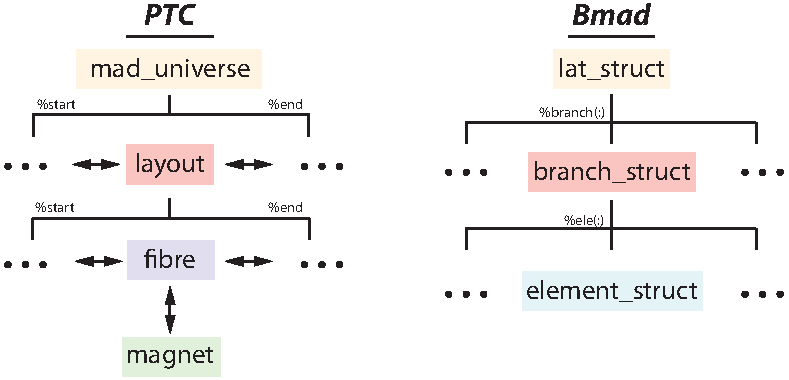
\includegraphics{ptc-structures.pdf}
  \caption[PTC structure relationships] { 
Simplified diagram showing the organization of the major PTC structures involved in
defining a lattice contrasted with \bmad.
  }
\label{f:ptc-struct}
\end{figure}

%--------------------------------------------------------------------------
\section{Variable Initialization and Finalization}
\label{s:ptc.var.init}
\index{PTC/FPP variable!initialization}

PTC variables must be initialized and finalized. This is done with
the\vn{alloc()} and \vn{kill()} routines. In addition, the \vn{real_8_init}
routine can initialize a \vn{real_8} array:
\begin{example}
  type (real_8) y8(6) 
  ...
  call real_8_init (y8)
  call kill (y8)
\end{example}

%--------------------------------------------------------------------------
\section{Correspondence Between Bmad Elements and PTC Fibres}.
\label{s:ele.fib}
\index{fibre}

When a PTC \vn{layout} is created from a \bmad \vn{lat_struct}
instance using the routine
\Hyperref{r:lat.to.ptc.layout}{lat_to_ptc_layout}, the correspondence
between the \bmad elements and the PTC fibres is maintained through
the \vn{ele%ptc_fibre} pointer. The following rules apply:
  \begin{enumerate}
  \item There will be marker \vn{fibre}s at the beginning and end 
of the \vn{layout}. The beginning \vn{fibre} will correspond to
\vn{branch%ele(0)}. The end \vn{fibre} will not have a corresponding
\bmad element.
  \item Generally there will be a one-to-one correspondence between
\vn{fibre}s and \vn{branch%ele} elements. The exception is where a
``hard edge'' model is used for tracking. In this case, there will be
three \vn{fibre}s for the \bmad element: Two drift \vn{fibre}s with a
\vn{fibre} of the appropriate type inbetween.  In this case,
\vn{ele%ptc_fibre} will point to the last (drift) \vn{fibre}.
  \end{enumerate}

Remember: The attributes like reference energy, etc. for a \bmad
\vn{ele_struct} instance are referenced to the exit end of the
element. For PTC the reference edge for a \vn{fibre} is the entrance
end.

%--------------------------------------------------------------------------
\section{Taylor Maps}
\label{s:ptc.taylor}
\index{PTC/FPP!Taylor Maps}

\index{PTC/FPP!real_8}\index{PTC/FPP!universal_taylor}
FPP stores its \vn{real_8} Taylor maps in such a way that it is not
easy to access them directly to look at the particular terms. To
simplify life, \'Etienne has implemented the
\vn{universal_taylor}structure:
\begin{example}
  type universal_taylor
    integer, pointer  :: n       ! Number of coefficients
    integer, pointer  :: nv      ! Number of variables
    real(dp), pointer :: c(:)    ! Coefficients C(N)
    integer, pointer  :: j(:,:)  ! Exponents of each coefficients J(N,NV)
  end type
\end{example}
\bmad always sets \vn{nv} = 6. \bmad overloads the equal sign to call 
routines to convert between \'Etienne's
\vn{real_8} Taylor maps and \vn{universal_taylor}:
\begin{example}
  type (real_8) tlr(6)           ! Taylor map
  type (universal_taylor) ut(6)  ! Taylor map
  ...
  tlr = ut                       ! Convert universal_taylor -> real_8
  ut = tlr                       ! Convert real_8 -> universal_taylor
\end{example}

%--------------------------------------------------------------------------
\section{Patches}
\label{s:ptc.patch}
\index{PTC/FPP!patch}

There is a significant difference between how patches are treated in
PTC and \bmad.  In PTC, a patch is just though of as a coordinate
transformation for propagating a particle from one \vn{fibre} to the
next. As such, the \vn{patch} is part of a \vn{fibre}. That is, any
\vn{fibre} representing tracking through quadrupoles, bends, etc. will
have patches for the entrance and exit ends of the \vn{fibre}.

With \bmad, on the other hand, a \vn{patch} is a ``first class''
element on par with all other elements be they quadrupoles, bends,
etc. When translating a \vn{patch} from \bmad to PTC, the \vn{patch}
is represented in PTC as a \vn{marker} element with a patch at the
exit end.

%--------------------------------------------------------------------------
\section{Number of Integration Steps \& Integration Order}
\label{s:ptc.step}

``Drift like'' elements in PTC will use, by default, only one
integration step. \bmad uses the default when translating from \bmad
lattice elements to PTC fibres. The \bmad lattice elements that are
drift like are:
\begin{example}
  drift
  ecollimator 
  instrument 
  monitor 
  pipe
  rcollimator 
\end{example}

When tracking, there is a tradeoff between step size and integrator order. Higher order
means fewer steps are needed to get the same accuracy. But one higher order step is
computationally more intensive then one lower order step so what is the optimum order and
number of steps is dependent upon various factors like magnet strength and how fast the
field is varying. Generally, when the field is varying, such as in a wiggler, lower order
and more steps are favored. Also spin tracking is always 2nd order in PTC. So going to higher
order for the orbital tracking with less steps will cause the spin tracking to be less
accurate.

The way PTC ``resplitting'' routines work is that, for a given element, they start by
assuming that the tracking will be done using a 2\Nd order integrator, They then compute
the number of steps needed based upon the electric and magnetic field strengths. This
number is compared to a crossover limit point here named $C_1$. If the number of steps is
less than or equal to $C_1$ then the resplitting routine stops and tracking will
thereafter be done with a 2\Nd order integrator with the calculated number of steps. On
the other hand, if the number of steps is greater than $C_1$, the resplitting routine will
redo the calculation assuming 4\Th order integration. With 4\Th order integration, the
number of calculated steps will compared to a different crossover limit point here called
$C_2$. Again, if the number of steps is less than or equal to $C_2$, the routine will
assign 4\Th order tracking to the element. Otherwise, the routine will assign 6\Th order
tracking to the element with an appropriate number of steps.

The default crossover limit points are
\begin{align}
  [C_1, C_2] & = [30, 60] \qquad \text{For wiggler type elements.} \nonumber \\
  [C_1, C_2] & = [4, 18]  \qquad \text{For all other elements.} \nonumber 
\end{align}
The greater number for wigglers is a reflection of the fact that the wiggler field
is not constant.


%% PTC: defines real(8), real_8, probe, probe_8 
%% FPP: defines damap and c_damap and gmap
%% PTC only uses damap and c_damap for analysis not tracking.

\chapter{OPAL}
\label{c:opal}
\index{OPAL}
%----------------------------------------------------------------------------

OPAL (Object Oriented Parallel Accelerator Library) is a tool for charged-particle optic calculations in large accelerator structures and beam lines including 3D space charge. OPAL is built from first principles as a parallel application, OPAL admits simulations of any scale: on the laptop and up to the largest High Performance Computing (HPC) clusters available today. Simulations, in particular HPC simulations, form the third pillar of science, complementing theory and experiment.

OPAL includes various beam line element descriptions and methods for single particle optics, namely maps up to arbitrary order, symplectic integration schemes and lastly time integration. OPAL is based on IPPL (Independent Parallel Particle Layer) which adds parallel capabilities. Main functions inherited from IPPL are: structured rectangular grids, fields and parallel FFT and particles with the respective interpolation operators. Other features are, expression templates and massive parallelism (up to 8000 processors) which makes is possible to tackle the largest problems in the field.


The  manual can be obtained at
\begin{example} 
  <http://amas.web.psi.ch/docs/opal/>    
\end{example}


%--------------------------------------------------------------------------
\section{Phase Space}
\label{s:opal.space}
\index{OPAL!phase space}

OPAL uses different longitudinal phase space coordinates compared to \bmad.
\bmad's phase space coordinates are
\Begineq
  (x, p_x/p_0, y, p_y/p0, -\beta c (t - t_0), (p-p_0)/p_0)
\Endeq
OPAL uses
\Begineq
  (x, \gamma \beta_x,  y, \gamma \beta_y, z, \gamma \beta_z)
\Endeq
\vn{convert_particle_coordinates_s_to_t} and \vn{convert_particle_coordinates_s_to_t} are conversion routines \ldots

%%--------------------------------------------------------------------------
%\section{Initialization}
%\label{s:etienne.init}
%\index{PTC/FPP!initialization}
%
%One important parameter in PTC is the order of the Taylor maps.
%By default \bmad will set this to 3. The order can be set within
%a lattice file using the \vn{parameter[taylor_order]} attribute.
%In a program the order can be set using \vn{set_ptc}. In fact
%\vn{set_ptc} must be called by a program before PTC can be used.
%\vn{bmad_parser} will do this when reading in a lattice file.
%That is, if a program does not use \vn{bmad_parser} then to use PTC it
%must call \vn{set_ptc}. Note that resetting PTC to a different order
%reinitializes PTC's internal memory so one must be careful if one wants
%to change the order in mid program.
%
%%--------------------------------------------------------------------------
%\section{Taylor Maps}
%\label{s:etienne.taylor}
%\index{PTC/FPP!Taylor Maps}
%
%\index{PTC/FPP!real_8}\index{PTC/FPP!universal_taylor}
%FPP stores its \vn{real_8} Taylor maps in such a way that it is not
%easy to access them directly to look at the particular terms. To
%simplify life, \'Etienne has implemented the
%\vn{universal_taylor}structure:
%\begin{example}
%  type universal_taylor
%    integer, pointer  :: n       ! Number of coefficients
%    integer, pointer  :: nv      ! Number of variables
%    real(dp), pointer :: c(:)    ! Coefficients C(N)
%    integer, pointer  :: j(:,:)  ! Exponents of each coefficients J(N,NV)
%  end type
%\end{example}
%\bmad always sets \vn{nv} = 6. \bmad overloads the equal sign to call 
%routines to convert between \'Etienne's
%\vn{real_8} Taylor maps and \vn{universal_taylor}:
%\begin{example}
%  type (real_8) tlr(6)           ! Taylor map
%  type (universal_taylor) ut(6)  ! Taylor map
%  ...
%  tlr = ut                       ! Convert universal_taylor -> real_8
%  ut = tlr                       ! Convert real_8 -> universal_taylor
%\end{example}

\chapter{C++ Interface}
\label{c:cpp.interface}
\index{C++ interface}

To ease the task of using \cpp routines with \bmad, there is a
library called \vn{cpp_bmad_interface} which implements a set of \cpp
classes in one--to--one correspondence with the major \bmad
structures. In addition to the \cpp classes, the \bmad library
defines a set of conversion routines to transfer data values between
the \bmad Fortran structures and the corresponding \cpp classes.

The list of all classes is given in the file
\begin{example}
  cpp_bmad_interface/include/cpp_bmad_classes.h
\end{example}
The general rule is that the equivalent class to a \bmad structure
named \vn{xxx_struct} will be named \vn{CPP_xxx}. Additionally, for
each \bmad structure, there is a opaque class named \vn{Bmad_xxx_class}
for use in the translation code discussed below. The names of these
opaque classes have the form \vn{Bmad_xxx_class} and are used to define
pointer instances in routine argument lists.

%----------------------------------------------------------------------------
\section{C++ Classes and Enums}
\index{C++ interface!classes}

Generally, The \cpp classes have been set up to simply mirror the
corresponding \bmad structures. For example, the \vn{CPP_lat} class
has a string component named \vn{.version} that mirrors the
\vn{%version} component of the \vn{lat_struct} structure. There are
some exceptions. For example, structure components that are part of
\vn{PTC} (\sref{s:ptc.intro}) are not present in the classes.

While generally the same component name is used for both the \bmad
structures and the \cpp classes, in the case where there is a \cpp
reserved word conflict, the \cpp component name will be different.

A header file \vn{bmad_enums.h} defines corresponding \bmad
parameters for all \cpp routine. The \bmad parameters are in a
namespace called \vn{Bmad}. The convention is that the name of a
corresponding \cpp parameter is obtained by dropping the ending
\vn{\$} (if there is one) and converting to uppercase. For example,
\vn{electron\$} on the Fortran side converts to \vn{Bmad::ELECTRON} in
\cpp. 

All of the \cpp class components that are arrays or matrices are zero
based so that, for example, the index of the \vn{.vec[i]} array in a
\vn{CPP_coord} runs from 0 through 5 and not 1 through 6 as on the
Fortran side. Notice that for a \vn{lat_struct} the \vn{%ele(0:)}
component has a starting index of zero so there is no off--by--one
problem here.  The exception to this rule is the \vn{%value(:)} array
of the \vn{ele_struct} which has a span from 1 to
\vn{num_ele_attrib\$}. In this case, To keep the conversion of the of
constructs like \vn{ele%value(k1\$)} consistant, the corresponding
\vn{ele.value[]} array has goes from 0 to \vn{Bmad::NUM_ELE_ATTRIB}
with the 0th element being unused.

%----------------------------------------------------------------------------
\section{Conversion Between Fortran and C++}
\index{C++ interface!Fortran calling C++}

\begin{figure}[tb]
\begin{listing}{1}
  subroutine f_test
    use bmad_cpp_convert_mod
    implicit none

    interface
      subroutine cpp_routine (f_lat, c_coord) bind(c)
        import f_lat, c_ptr
        type (lat_struct) :: f_lat
        type (c_ptr), value :: c_coord
      end subroutine
    end interface

    type (lat_struct), target :: lattice   // lattice on Fortran side 
    type (coord_struct), target :: orbit
    type (c_ptr), value :: c_lat
    ! ... 
    call lat_to_c (c_loc(lattice), c_lat)    ! Fortran side convert
    call cpp_routine (c_lat, c_loc(orbit))   ! Call C++ routine
    call lat_to_f (c_lat, c_loc(lattice))    ! And convert back
  end subroutine
\end{listing}
\caption{Example Fortran routine calling a \cpp routine.}
\label{f:fortran}
\end{figure}


\begin{figure}
\begin{listing}{1}
  #include "cpp_bmad_classes.h"

  using namespace Bmad;

  extern "C" cpp_routine (CPP_lat& c_lat, Bmad_coord_class* f_coord,  f_lat) {
    CPP_coord c_coord;
    coord_to_c (f_coord, c_coord);        // C++ side convert
    // ... do calculations ...
    cout << c_lat.name << "  " << c_lat.ele[1].value[K1] << endl;
    coord_to_f (c_coord, f_coord);        // And convert back
  }
\end{listing}
\caption{Example \cpp routine callable from a Fortran routine.}
\label{f:cpp}
\end{figure}

A simple example of a Fortran routine calling a \cpp routine is shown
in \figs{f:fortran} and \ref{f:cpp}. Conversion between structure and
classes can happen on either the Fortran side or the \cpp side. In
this example, the \vn{lat_struct} / \vn{CPP_lat} conversion is on the
Fortran side and the \vn{coord_struct} / \vn{CPP_coord} is on the \cpp
side. 

On the Fortran side, the interface block defines the argument list of
the \cpp routine being called.

On the \cpp side, \vn{f_coord} is an instance of the
\vn{Bmad_coord_class} opaque class.

A \cpp routine calling a Fortran routine has a similar structure to
the above example. The interface block in \fig{f:fortran} can be used
as a prototype. For additional examples of conversion between Fortran
and \cpp, look at the test code in the directory
\begin{example}
  cpp_bmad_interface/interface_test
\end{example}

\chapter{Quick_Plot Plotting}
\label{c:quick.plot}
\index{quick_plot|hyperbf}
\index{pgplot!and Quick_Plot}

The plotting package included in the \bmad distribution is PGPLOT
(see \sref{s:libs}).
One drawback of PGPLOT is that the arguments to
PGPLOT's subroutines are not always conveniently structured. to remedy
this a suite of wrapper routines have been developed which can be
used to drive PGPLOT. This suite is called \quickplot and lives in the
\vn{sim_utils} library which comes with the Bmad distribution. A quick
reference guide can be seen online by using the command \vn{getf
quick_plot}. For quick identification in a program, all \quickplot
subroutines start with a \vn{qp_} prefix. Also, by convention, all
PGPLOT subroutines start with a \vn{pg} prefix.

While \quickplot covers most of the features of PGPLOT, \quickplot is
still a work in progress.  For example, contour plots have not yet
been implemented in \quickplot. If you see a feature that is lacking
in \quickplot please do not hesitate to make a request to
\vn{dcs16@cornell.edu}.

Note: PGPLOT uses single precision real(4) numbers while \quickplot
uses real(rp) numbers.  If you use any PGPLOT subroutines directly be
careful of this.

%----------------------------------------------------------------------------

\begin{figure}
\index[routine]{qp_open_page}
\index[routine]{qp_close_page}
\index[routine]{qp_read_data}
\index[routine]{qp_calc_and_set_axis}
\index[routine]{qp_draw_text}
\index[routine]{qp_draw_axes}
\index[routine]{qp_draw_data}
\index[routine]{qp_save_state}
\index[routine]{qp_restore_state}
\index[routine]{qp_set_page_border}
\index[routine]{qp_set_margin}
\index[routine]{qp_set_line_attrib}
\index[routine]{qp_set_box}
\index[routine]{qp_set_graph_attrib}
\index[routine]{qp_set_symbol_attrib}
\index[routine]{qp_set_axis}
\footnotesize
\begin{listing}{1}
  program example_plot
    use quick_plot
    integer id
    character(1) ans
  
    ! Generate PS and X-windows plots.
    call qp_open_page ("PS-L")  ! Tell \quickplot to generate a PS file.
    call plot_it              ! Generate the plot
    call qp_close_page        ! quick_plot.ps is the file name
    call qp_open_page ("X", id, 600.0_rp, 470.0_rp, "POINTS")
    call plot_it
    write (*, "(a)", advance = "NO") " Hit any class to end program: "
    accept "(a)", ans

  !----------------------------------------------------------------------
  contains
  subroutine plot_it                             ! This generates the plot
    real(rp), allocatable :: x(:), y(:), z(:), t(:)
    real(rp) x_axis_min, x_axis_max, y_axis_min, y_axis_max
    integer x_places, x_divisions, y_places, y_divisions
    character(80) title
    logical err_flag
    namelist / parameters / title

    ! Read in the data
    open (1, file = "plot.dat", status = "old")
    read (1, nml = parameters)                  ! read in the parameters.
    call qp_read_data (1, err_flag, x, 1, y, 3, z, 4, t, 5) ! read in the data.
    close (1)

    ! Setup the margins and page border and draw the title
    call qp_set_page_border (0.01_rp, 0.02_rp, 0.2_rp, 0.2_rp, "%PAGE")
    call qp_set_margin (0.07_rp, 0.05_rp, 0.05_rp, 0.05_rp, "%PAGE")
    call qp_draw_text (title, 0.5_rp, 0.85_rp, "%PAGE", "CT") 

    ! draw the left graph
    call qp_set_box (1, 1, 2, 1)
    call qp_calc_and_set_axis ("X", minval(x), maxval(x), 4, 8, "ZERO_AT_END")
    call qp_calc_and_set_axis ("Y", minval(z), maxval(z), 4, 8, "GENERAL")
    call qp_draw_axes ("X\dlab\u", "\gb(\A)")
    call qp_draw_data (x, y, symbol_every = 0)

    call qp_save_state (.true.)
    call qp_set_symbol_attrib (times$, color = blue$, height = 20.0_rp)
    call qp_set_line_attrib ("PLOT", color = blue$, style = dashed$)
    call qp_draw_data (x, z, symbol_every = 5)
    call qp_restore_state

    ! draw the right graph. star5_filled$ is a five pointed star.
    call qp_save_state (.true.)
    call qp_set_box (2, 1, 2, 1)
    call qp_set_graph_attrib (draw_grid = .false.)
    call qp_set_symbol_attrib (star5_filled$, height = 10.0_rp)
    call qp_set_axis ("Y", -0.1_rp, 0.1_rp, 4, 2)
    call qp_set_axis ('Y2', 1.0_rp, 100.0_rp, label = 'Y2 axis', &
                                draw_numbers = .true., ax_type = 'LOG')
    call qp_draw_axes ("\m1 \m2 \m3 \m4 \m5 \m6 \m7", "\fsLY\fn", title = "That Darn Graph")
    call qp_draw_data (x, t, draw_line = .false., symbol_every = 4)
    call qp_restore_state
  end subroutine
  end program
\end{listing}
\caption{\quickplot example program.}
\label{f:plot.example}
\end{figure}


\begin{figure}
\centering
\includegraphics[angle=-90,width=5.5in]{plot-example.pdf}
\caption{Output of plot_example.f90.}
\label{f:plot.out}
\end{figure}

%----------------------------------------------------------------------------
\section{An Example}
\label{s:plot.example}

An example of how \quickplot can be used in a program is shown in
\fig{f:plot.example}. In the \bmad distribution a copy of this
program is in the file
\begin{example}
  sim_utils/plot_example/plot_example.f90
\end{example}
The \vn{plot_example.f90} program generates the figure shown in
\fig{f:plot.out} from the input file named \vn{plot.dat}. The
first few lines of the data file are
\begin{example}
  \&parameters
    title = "A Tale of Two Graphs"
  /
 
  Any junk here...
 
  Col1      Col2      Col3      Col4      Col5
     0    0.0000    0.1000    0.0000   -0.0125
     1    0.0001    0.0995    0.0101   -0.0127
     2    0.0004    0.0980    0.0203   -0.0130
     3    0.0009    0.0955    0.0304   -0.0132
     ...
\end{example}

The program first creates a PostScript file for printing on lines 7
through 9 and then makes an X--windows plot on lines 10 and 11. The
write/accept lines 12 and 13 are to pause the program to prevent the
X-window from immediately closing upon termination of the program.

The heart of the plotting is in the subroutine \vn{plot_it} beginning
on line 17. The namelist read on line 27 shows how both parameters and
data can be stored in the same file so that a plotting program can be
automatically told what the appropriate plot labels are. The
\Hyperref{r:qp.draw.text}{qp_draw_text} call on line 34 draws the 
title above the two graphs.

The \Hyperref{r:qp.read.data}{qp_read_data} call on line 28 will skip
any ``header'' lines (lines that do not begin with something that looks
like a number) in the data file. In this instance
\Hyperref{r:qp.read.data}{qp_read_data} will read the first, third forth
and fifth data columns and put them into the \vn{x}, \vn{y}, \vn{z}, and
\vn{t} arrays.

\Hyperref{r:qp.set.page.border}{qp_set_page_border},
\Hyperref{r:qp.set.box}{qp_set_box}, and
\Hyperref{r:qp.set.margin}{qp_set_margin} sets where the graph is
going to be placed.  \Hyperref{r:qp.set.box}{qp_set_box}\vn{(1, 1, 2,
1)} on line 37 tells \quickplot to put the first graph in the left box
of a 2 box grid. The \Hyperref{r:qp.set.margin}{qp_set_margin} on line
33 sets the margins between the box and the graph axes.

\Hyperref{r:qp.calc.and.set.axis}{qp_calc_and_set_axis} on lines 38
and 39 are used to scale the axes. \vn{"ZERO_AT_END"} ensures that the
$x$--axis starts (or stops) at zero.
\Hyperref{r:qp.calc.and.set.axis}{qp_calc_and_set_axis} is told to
restrict the number of major divisions to be between 4 and 8. For the
horizontal axis, as can be seen in \fig{f:plot.out}, it chooses
5 divisions.

After drawing the first data curve (the solid curve) in the left
graph, the routines
\Hyperref{r:qp.set.symbol.attrib}{qp_set_symbol_attrib} and
\Hyperref{r:qp.set.line.attrib}{qp_set_line_attrib} are called on
lines 44 and 45 to plot the next data curve in blue with a dashed line
style. By default, this curve goes where the last one did: in the left
graph. To keep the setting of the line and symbol attributes from
affecting other plots the routines
\Hyperref{r:qp.save.state}{qp_save_state} and
\Hyperref{r:qp.restore.state}{qp_restore_state} on lines 43 and 47 are
used. \Hyperref{r:qp.save.state}{qp_save_state} saves the current
attributes in an attribute
stack. \Hyperref{r:qp.restore.state}{qp_restore_state} restores the
saved attributes from the attribute
stack. \Hyperref{r:qp.draw.axes}{qp_draw_axes} is called on line 40 to
draw the $x$ and $y$-axes along, and \vn{qp_draw_data} is called on
lines 41 and 46 to draw the two data curves.

Lines 50 through 60 draw the third curve in the right hand graph.  The
\vn{qp_set_axis} call on lines 55/56 sets a log scale for the \vn{y2}
(right hand) axis. The syntax of the string arguments of
\Hyperref{r:qp.draw.axes}{qp_draw_axes} in lines 40 and 57/58 comes from PGPLOT and allows
special symbols along with subscripts and superscripts.

%----------------------------------------------------------------------------
\section{Plotting Coordinates}
\label{s:plot.coords}

\begin{figure}
  \centering
  \includegraphics{plot-coords.pdf}
  \caption{A Graph within a Box within a Page.}
  \label{f:plot.coords}
\end{figure}

\quickplot uses the following concepts as shown in \fig{f:plot.coords}
\begin{example}
  PAGE  -- The entire drawing surface.
  BOX   -- The area of the page that a graph is placed into.
  GRAPH -- The actual plotting area within the bounds of the axes.
\end{example}
In case you need to refer to the PGPLOT routines the correspondence
between this and PGPLOT is:
\begin{example}
  QUICK_PLOT    PGPLOT
  ----------    ------
  PAGE          VIEW SURFACE
  BOX           No corresponding entity.
  GRAPH         VIEWPORT and WINDOW
\end{example}
Essentially the VIEWPORT is the region outside of which lines and symbols
will be clipped (if clipping is turned on) and the WINDOW defines the
plot area. I'm not sure why PGPLOT makes a distinction, but VIEWPORT and
WINDOW are always the same region.

\Hyperref{r:qp.open.page}{qp_open_page} determines the size of the \vn{page} if it is
settable (like for X--windows). The page is divided up into a grid of
boxes. For example, in \fig{f:plot.coords}, the grid is 1 box
wide by 3 boxes tall. The border between the grid of boxes and the
edges of the page are set by \Hyperref{r:qp.set.page.border}{qp_set_page_border}.  The box that
the graph falls into is set by \Hyperref{r:qp.set.box}{qp_set_box}. The default is to
have no margins with 1 box covering the entire page. The
\Hyperref{r:qp.set.margin}{qp_set_margin} routine sets the distance between the box edges
and the axes (See the PGPLOT manual for more details).


%----------------------------------------------------------------------------
\section{Length and Position Units}
\label{s:plot.units}
\index{quick_plot!position units}

Typically there is an optional \vn{units} argument for \quickplot routines that
have length and/or position arguments. For example, using \vn{getf} one can
see that the arguments for \Hyperref{r:qp.draw.rectangle}{qp_draw_rectangle} are
\begin{example}
  Subroutine qp_draw_rectangle (x1, x2, y1, y2, units, color, width, style, clip)
\end{example}
The \vn{units} argument is a character string which is divided into three
parts. The syntax of the \vn{units} argument is
\begin{example}
  unit_type/ref_object/corner
\end{example}
The first part \vn{unit_type} gives the type of units
\begin{example}
  "%"       -- Percent.
  "DATA"    -- Data units. (Draw default)
  "MM"      -- millimeters.
  "INCH"    -- Inches. (Set default)
  "POINTS"  -- Printers points (72 points = 1 inch, 1pt is about 1pixel).
\end{example}
The second and third parts give the reference point for a position.
The second part specifies the reference object
\begin{example}
    "PAGE"  -- Relative to the page (Set default).
    "BOX"   -- Relative to the box.
    "GRAPH" -- Relative to the graph (Draw default).
\end{example}
The third part gives corner of the reference object that is the reference point
\begin{example}
    "LB"    -- Left Bottom (Set and Draw default).
    "LT"    -- Left Top.
    "RB"    -- Right Bottom.
    "RT"    -- Right Top.
\end{example}

Notes:
\begin{itemize}
 \item 
The \vn{DATA} unit type, by definition, always uses the lower left
corner of the \vn{GRAPH} as a reference point.
 \item 
For the \vn{%} \vn{unit_type} the \vn{/} between \vn{unit_type} 
and \vn{ref_object} can be omitted.
 \item 
If the \vn{corner} is specified then the \vn{ref_object} must appear also.
 \item 
Everything must be in upper case.
 \item 
For some routines (\Hyperref{r:qp.set.margin}{qp_set_margin}, etc.) only a relative distance
is needed. In this case the \vn{ref_object/corner} part, if present,
is ignored.
 \item 
The \vn{units} argument is typically an optional argument. If not
present the default units will be used. There are actually two
defaults: The draw default is used for drawing text, symbols, or whatever.
The set default is used for setting margins, and other lengths.
Initially the draw default is \vn{DATA/GRAPH/LB} and the set
default is \vn{INCH/PAGE/LB}. 
Use \Hyperref{r:qp.set.parameters}{qp_set_parameters} to change this.
\end{itemize}
Examples:
\begin{example}
  "DATA"          -- This is the draw default. 
  "DATA/GRAPH/LB" -- Same as above.
  "DATA/BOX/RT"   -- ILLEGAL: DATA must always go with GRAPH/LB.
  "%PAGE/LT"      -- Percentage of page so (0.0, 1.0) = RT of page.
  "%BOX"          -- Percentage of box so (1.0, 1.0) = RT of box.
  "INCH/PAGE"     -- Inches from LB of page.
\end{example}

%----------------------------------------------------------------------------
\section{Y2 and X2 axes}
\label{s:axes2}
\index{quick_plot!axes}

The top and right axes of a graph are known as \vn{X2} and \vn{Y2}
respectively as shown in \fig{f:plot.coords}. Normally the
\vn{X2} axis mirrors the \vn{X} axis and the \vn{Y2} axis mirrors the
\vn{Y} axis in that the tick marks and axis numbering for the \vn{X2}
and \vn{Y2} axes are the same as the \vn{X} and \vn{Y} axes
respectively. \Hyperref{r:qp.set.axis}{qp_set_axis} can be used to disable mirroring. For
example:
\begin{example}
  call qp_set_axis ("Y2", mirror = .false.)  ! y2-axis now independent of y.
\end{example}
\Hyperref{r:qp.set.axis}{qp_set_axis} can also be used to set \vn{Y2} axis parameters
(axis minimum, maximum, etc.) and setting the \vn{Y2} or \vn{X2} axis
minimum or maximum will, by default, turn off mirroring.

Note that the default is for the \vn{X2} and \vn{Y2} axis numbering
not to be shown. To enable or disable axis numbering again use
\Hyperref{r:qp.set.axis}{qp_set_axis}. For example:
\begin{example}
  call qp_set_axis ("Y2", draw_numbers = .true.)  ! draw y2 axis numbers
\end{example}

To plot data using the \vn{X2} or \vn{Y2} scale use the
\Hyperref{r:qp.use.axis}{qp_use_axis} routine. For example:
\begin{example}
  call qp_save_state (.true.)
  call qp_use_axis (y = 'Y2')
  ! ... Do some data plotting here ...
  call qp_restore_state
\end{example}

%----------------------------------------------------------------------------
\section{Text}
\label{s:text}

PGPLOT defines certain escape sequences that can be used in text strings
to draw Greek letters, etc. These escape sequences are given in 
Table~\ref{t:pgplot.escape}.

PGPLOT defines a text background index:
\begin{example}
         -1 - Transparent background.
          0 - Erase underlying graphics before drawing text.
   1 to 255 - Opaque with the number specifying the color index.
\end{example}

%----------------------------------------------------------------------------
\section{Styles}
\label{s:styles}

Symbolic constants have been defined for \quickplot subroutine
arguments that are used to choose various styles. As an example of
this is in lines 44 and 45 of \fig{f:plot.example}. The
numbers in the following are the PGPLOT equivalents.

\index{quick_plot!line styles}
The \quickplot line styles are:
\begin{example}
    1 -- solid\$                  Solid
    2 -- dashed\$                 Dashed
    3 -- dash_dot\$               Dash--dot 
    4 -- dotted\$                 Dotted
    5 -- dash_dot3\$              Dash--dot--dot--dot        
\end{example}

\index{quick_plot!color styles}
The color styles in \quickplot are:
\begin{example}
    0 -- White\$   (actually the background color)
    1 -- Black\$   (actually the foreground color)
    2 -- Red\$
    3 -- Green\$
    4 -- Blue\$
    5 -- Cyan\$
    6 -- Magenta\$
    7 -- Yellow\$ 
    8 -- Orange\$
    9 -- Yellow_Green\$
   10 -- Light_Green\$
   11 -- Navy_Blue\$
   12 -- Purple\$
   13 -- Reddish_Purple\$
   14 -- Dark_Grey\$
   15 -- Light_Grey\$
\end{example}
   
Integers from [17, (largest integer)] represent continuous colors. The function \vn{pq_continuous_color} maps [0.0, 1.0] to these integers. See Fig.~\ref{f:plot-continuous-color}.

\begin{figure}
\centering
\includegraphics[width=0.8\textwidth]{plot-continuous-color.pdf}
\caption{Continuous colors using the function \vn{pg_continuous_color} in PGPlot and PLPlot. Typical usage: \vn{call qp_routine(..., color = pg_continuous_color(0.25_rp), ...)}}
\label{f:plot-continuous-color}
\end{figure}

\index{quick_plot!fill styles}
The fill styles are:
\begin{example}
    1 -- solid_fill\$        
    2 -- no_fill\$           
    3 -- hatched\$           
    4 -- cross_hatched\$     
\end{example}

\index{quick_plot!symbol styles}
The symbol types are:
\begin{example}
    0 -- square_sym\$
    1 -- dot_sym\$
    2 -- plus_sym\$
    3 -- times_sym\$
    4 -- circle_sym\$
    5 -- x_sym\$
    7 -- triangle_sym\$
    8 -- circle_plus_sym\$
    9 -- circle_dot_sym\$
   10 -- square_concave_sym\$
   11 -- diamond_sym\$
   12 -- star5_sym\$
   13 -- triangle_filled_sym\$
   14 -- red_cross_sym\$
   15 -- star_of_david_sym\$
   16 -- square_filled_sym\$
   17 -- circle_filled_sym\$
   18 -- star5_filled_sym\$
\end{example}
Beside this list, PGPLOT maps other numbers onto symbol types. 
The PGPLOT list of symbols is:
\begin{example}
  -3 ... -31 - a regular polygon with abs(type) edges.
          -2 - Same as -1.
          -1 - Dot with diameter = current line width.
   0 ...  31 - Standard marker symbols.
  32 ... 127 - ASCII characters (in the current font).
                  E.G. to use letter F as a marker, set type = ICHAR("F"). 
       > 127 - A Hershey symbol number.
\end{example}
Table~\ref{t:plot.syms} shows some of the symbols and there associated 
numbers. Note: At constant height PGPLOT gives symbols of different size.
To partially overcome this, \quickplot scales some of the symbols to
give a more uniform appearance. Table~\ref{t:plot.syms} was generated
using a height of 40 via the call
\begin{example}
  call qp_draw_symbol (0.5_rp, 0.5_rp, "%BOX", k, height = 40.0_rp)
\end{example}

\index{quick_plot!symbol table}
\begin{table}
  \centering
  \includegraphics{plot-syms.pdf}
  \caption{Plotting Symbols at Height = 40.0}
  \label{t:plot.syms}
\end{table}

\begin{table}
\begin{tabular}{ll} \toprule
{\B}u       & Start a superscript or end a subscript \\[0.5ex]
{\B}d       & Start a subscript or end a superscript.
              {\B}u and {\B}d must always be used in pairs \\[0.5ex]
{\B}b       & Backspace (i.e., do not advance text pointer  
               after plotting the previous character) \\[0.5ex]
{\B}fn      & Switch to Normal font (1)       \\[0.5ex]
{\B}fr      & Switch to Roman font (2)        \\[0.5ex]
{\B}fi      & Switch to Italic font (3)       \\[0.5ex]
{\B}fs      & Switch to Script font (4)       \\[0.5ex]
{\B}{\B}    & Backslash character (\B)        \\[0.5ex]
{\B}x       & Multiplication sign ($\times$)  \\[0.5ex]
{\B}.       & Centered dot ($\cdot$)          \\[0.5ex]
{\B}A       & Angstrom symbol (\AA)         \\[0.5ex]
{\B}gx      & Greek letter corresponding to roman letter x \\[0.5ex]
{\B}mn {\B}mnn & Graph marker number $n$ or $nn$ (1-31) \\[1ex]
{\B}(nnnn)  & 
\parbox{4.8in}{\setstretch{0.5} Character number nnnn (1 to 4 decimal digits) from the
Hershey character set; the closing parenthesis may be omitted if the
next character is neither a digit nor ``)''. This makes a number of
special characters (e.g., mathematical, musical, astronomical, and
cartographical symbols) available.} \\ \bottomrule
\end{tabular}
\caption{PGPLOT Escape Sequences.}
\label{t:pgplot.escape}
\end{table}

Table~\ref{t:greek} shows how the character string \vn{"{\B}g<r>"}, where \vn{"<r>"} 
is a Roman letter, map onto the Greek character set.
\begin{table}
  \centering
  \includegraphics[width=5.5in]{greek.pdf}
  \caption[Roman to Greek Character Conversion]{Conversion for the string 
\vn{"{\B}g<r>"} where \vn{"<r>"} is a Roman character to the corresponding 
Greek character.}
\label{t:greek}
\end{table}


%----------------------------------------------------------------------------
\section{Structures}
\label{s:qp.structs}
\index{quick_plot!structures}

\index{qp_line_struct}
\quickplot uses several structures to hold data. The structure that
defines a line is a \vn{qp_line_struct}
\begin{example}
  type qp_line_struct
    integer width   ! Line width. Default = 1
    integer color   ! Line color. Default = black\$
    integer style   ! Line style. Default = solid\$
  end type
\end{example}

\index{qp_symbol_struct}
The \vn{qp_symbol_struct} defines how symbols are drawn 
\begin{example}
  type qp_symbol_struct
    integer  type        ! Default = circle_dot\$
    real(rp) height      ! Default = 6.0 (points)
    integer  color       ! Default = black\$
    integer  fill        ! Default = solid_fill\$
    integer  line_width  ! Default = 1
  end type
\end{example}

\index{qp_axis_struct}
The \vn{qp_axis_struct} defines how axes are drawn 
\begin{example}
  type qp_axis_struct
    character(80) label       ! Axis label.
    real(rp) min              ! Axis range left/bottom number.
    real(rp) max              ! Axis range right/top number.
    real(rp) number_offset    ! Offset in inches of numbering from the axis line. 
                              !  Default = 0.05
    real(rp) label_offset     ! Offset in inches of the label from the numbering.
                              !  Default = 0.05
    integer label_color       ! black\$ (default), red\$, etc. 
    real(rp) major_tick_len   ! Length of the major ticks in inches. Def = 0.10
    real(rp) minor_tick_len   ! Length of the minor ticks in inches. Def = 0.06
    integer major_div         ! Number of major divisions. Default = 5
    integer major_div_nominal ! Nominal value. Def = 5.
    integer minor_div         ! Number of minor divisions. 0 = auto-choose. Default = 0
    integer minor_div_max     ! Maximum number for auto choose. Default = 5
    integer places            ! Places after the decimal point. Default = 0
    character(16) type        ! 'LINEAR' (default), 'LOG', or 'CUSTOM'.
    character(16) bounds      ! 'GENERAL' (default), 'ZERO_AT_END', ZERO_SYMMETRIC.
    integer tick_side         ! +1 = draw to the inside (def), 0 = both, -1 = outside.
    integer number_side       ! +1 = draw to the inside, -1 = outside (default).
    logical draw_label        ! Draw the label? Default = True.
    logical draw_numbers      ! Draw the numbering? Default = True.
  end type
\end{example}

\begin{example}
  type qp_plot_struct
    character(80) :: title = ' '
    type (qp_axis_struct) x, y, x2, y2
    type (qp_axis_struct), pointer :: xx, yy  ! Pointer to axes used for plotting.
    logical :: draw_box    = .true.
    logical :: draw_title  = .true.
    logical :: draw_grid   = .true.
    logical :: x2_mirrors_x = .true.
    logical :: y2_mirrors_y = .true.
    logical :: xx_points_to_x
    logical :: yy_points_to_y
  end type
\end{example}

%\end{document}

\chapter{Helper Routines}
\label{c:helper}

This chapter gives an overview of various computational helper routines.

%-----------------------------------------------------------------------------
\section{Nonlinear Optimization}
\label{s:opti}
\index{optimizers}

\index{numerical recipes!library}
\index{tao}
Nonlinear optimization is the process of finding a minimum (or
maximum) of a nonlinear function (the "merit" function). Nonlinear
optimization is frequently used for lattice design or matching of data
to a model. For more information on this see the \tao manual.

In terms of routines for implementing nonlinear optimization the
Numerical Recipes library (\sref{s:libs} that is distributed along
with \bmad contains several. In particular, 
the routine \Hyperref{r:super.mrqmin}{super_mrqmin}
which implements the Levenberg--Marquardt is an excellent routine for
finding local minimum when the merit function can be expressed as the
sum of quadratic terms. Another routine, \vn{frprmn}, which is an
implementation of the Fletcher--Reeves algorithm, is also good at
finding local minimum and has the advantage that as input it does not
need a derivative matrix as does Levenberg--Marquardt. The
disadvantage of Fletcher--Reeves is that it is slower than
Levenberg--Marquardt. 

A second implementation of Levenberg--Marquardt available with \bmad
is \Hyperref{r:opti.lmdif}{opti_lmdif} which is Fortran90 version of the popular
\vn{lmdif} routine. Also available is \Hyperref{r:opti.de}{opti_de} which implements
the Differential Evolution algorithm of Storn and
Price\cite{b:de}. This routine is good for finding global minima
but can be slow. 

Another routine that should be mentioned is the \vn{amoeba} routine
from Numerical Recipes that implements the downhill simplex method of
Neider and Mead. This routine is robust but slow but is easily
parallelized so it is a good routine for parallel processing.

%-----------------------------------------------------------------------------
\section{Matrix Manipulation}
\label{s:matrix}
\index{matrix manipulation}

There are a number of \bmad routines for matrix manipulation as listed
in \sref{r:mat}. In fact, Fortran90 has a number of intrinsic matrix
routines as well but this is outside the scope of this manual. The
following example shows some of the \bmad matrix routines
\Hyperref{r:mat.inverse}{mat_inverse}
\Hyperref{r:mat.make.unit}{mat_make_unit}
\begin{example}
  real(rp) mat(6,6), mat_inv(6,6)
  call mat_make_unit (mat)    ! make a unit matrix
  call mat_inverse (mat, mat_inv) ! Compute the inverse matrix.
\end{example}
\chapter{Bmad Library Routine List}

Below are a list of \bmad and sim_utils routines sorted by their
functionality.  Use the \vn{getf} and \vn{listf} (\sref{s:getf})
scripts for more information on individual routines.
This list includes low level routines that are not generally used in
writing code for a program but may be useful in certain unique
situations.  Excluded from the list are very low level routines that are
solely meant for \bmad internal use.

\toffset
\begin{center}
\begin{tabular}{ll} \toprule
{\em Routine Type} & {\em Section} \\ \midrule
  Beam: Low Level Routines                    & \ref{r:low.beam}       \\
  Beam: Tracking and Manipulation             & \ref{r:beam}           \\
  Branch Handling                             & \ref{r:branch}         \\
  Coherent Synchrotron Radiation (CSR)        & \ref{r:csr}            \\
  Collective Effects                          & \ref{r:collective}     \\
  Custom and Hook Routines                    & \ref{r:custom}         \\
  Electro-Magnetic Fields                     & \ref{r:em.fields}      \\
  Helper Routines: File, System, and IO       & \ref{r:helper.file}    \\
  Helper Routines: Math (Except Matrix)       & \ref{r:helper.math}    \\
  Helper Routines: Matrix                     & \ref{r:helper.matrix}  \\
  Helper Routines: Miscellaneous              & \ref{r:helper.misc}    \\
  Helper Routines: String Manipulation        & \ref{r:helper.string}  \\
  Helper Routines: Switch to Name             & \ref{r:switch}         \\
  Inter-Beam Scattering (IBS)                 & \ref{r:ibs}            \\
  Lattice: Informational                      & \ref{r:info}           \\
  Lattice: Element Manipulation               & \ref{r:elem}           \\
  Lattice: Geometry                           & \ref{r:geom}           \\
  Lattice: Low Level Stuff                    & \ref{r:lat.low}        \\
  Lattice: Manipulation                       & \ref{r:trans}          \\
  Lattice: Miscellaneous                      & \ref{r:lat.misc}       \\
  Lattice: Reading and Writing Files          & \ref{r:read}           \\
  Matrices                                    & \ref{r:mat}            \\
  Matrix: Low Level Routines                  & \ref{r:low.mat}        \\
  Measurement Simulation Routines             & \ref{r:meas}           \\
  Multipass                                   & \ref{r:multipass}      \\
  Multipoles                                  & \ref{r:multipoles}     \\
  Optimizers (Nonlinear)                      & \ref{r:opti}           \\
  Overload Equal Sign                         & \ref{r:equal}          \\
  Particle Coordinate Stuff                   & \ref{r:coord}          \\
  Photon Routines                             & \ref{r:photon}         \\
  PTC Interface                               & \ref{r:ptc}            \\
  Quick Plot                                  & \ref{r:qp}             \\
  Spin                                        & \ref{r:spin}           \\
  Transfer Maps: Routines Called by make_mat6 & \ref{r:mat6}           \\
  Transfer Maps: Complex Taylor Maps          & \ref{r:ctaylor}        \\
  Transfer Maps: Taylor Maps                  & \ref{r:taylor}         \\
  Tracking: Tracking and Closed Orbit         & \ref{r:track}          \\
  Tracking: Low Level Routines                & \ref{r:low.track}      \\
  Tracking: Mad Routines                      & \ref{r:mad}            \\
  Tracking: Routines Called by track1         & \ref{r:track1}         \\
  Twiss and Other Calculations                & \ref{r:twiss}          \\
  Twiss: 6-Dimensional                        & \ref{r:twiss6}         \\
  Wake Fields                                 & \ref{r:wake}           \\
  C/C++ Interface                             & \ref{r:c.interface}    \\
  % Deprecated                                & \ref{r:deprecated}     \\ \bottomrule
\end{tabular}
\end{center}
\toffset

%------------------------------------------------------------------------
\section{Beam: Low Level Routines}
\label{r:low.beam}

The following helper routines are generally not useful for general use.

\begin{description}

\index[routine]{bend_edge_kick}
\label{r:bend.edge.kick}
\item[bend_edge_kick (ele, param, particle_at, orb, mat6, make_matrix, track_spin)] \Newline 
Subroutine to track through the edge field of an sbend.
Reverse tracking starts with the particle just outside the bend and

\index[routine]{find_bunch_sigma_matrix}
\label{r:find.bunch.sigma.matrix}
\item[find_bunch_sigma_matrix (particle, charge, bunch_params, sigma_s)] \Newline 
Routine to find the sigma matrix elements of a particle distribution.

\index[routine]{init_spin_distribution}
\label{r:init.spin.distribution}
\item[init_spin_distribution (beam_init, bunch)] \Newline 
Initializes a spin distribution according to init_beam\%spin

\index[routine]{order_particles_in_z}
\label{r:order.particles.in.z}
\item[order_particles_in_z (bunch)] \Newline 
Routine to order the particles longitudinally in terms of decreasing \%vec(5).
That is from large z (head of bunch) to small z.

\index[routine]{track1_beam}
\label{r:track1.beam}
\item[track1_beam (beam_start, lat, ele, beam_end, err, centroid, direction)] \Newline 
Routine to track a beam of particles through a single element.
Overloaded by \vn{track1_beam}.

\index[routine]{track1_bunch}
\label{r:track1.bunch}
\item[track1_bunch (bunch_start, lat, ele, bunch_end, err, centroid, direction)] \Newline 
Routine to track a bunch of particles through an element.

\index[routine]{track1_bunch_hom}
\label{r:track1.bunch.hom}
\item[track1_bunch_hom (bunch_start, ele, param, bunch_end, direction)] \Newline 
Routine to track a bunch of particles through an element.

\end{description}

%------------------------------------------------------------------------
\section{Beam: Tracking and Manipulation}
\label{r:beam}    
\index{beam tracking!list of routines}

See \sref{s:part.track} for a discussion of using a collection of particles to simulate
a bunch.

\begin{description}

\index[routine]{bbi_kick}
\label{r:bbi.kick}
\item[bbi_kick (x_norm, y_norm, r, kx, ky)] \Newline 
Routine to compute the normalized kick due to the beam-beam
interaction using the normalized position for input.

\index[routine]{calc_bunch_params}
\label{r:calc.bunch.params}
\item[calc_bunch_params (bunch, bunch_params, err, print_err)] \Newline 
Finds all bunch parameters defined in bunch_params_struct, both normal-mode
and projected

\index[routine]{calc_bunch_params_slice}
\label{r:calc.bunch.params.slice}
\item[\protect\parbox{6in}{
    calc_bunch_params (bunch, bunch_params, plane, slice_center, \\
    \hspace*{1in} slice_spread, err, print_err) }] \Newline 
Finds all bunch parameters for a slice through the beam distribution.

\index[routine]{init_beam_distribution}
\label{r:init.beam.distribution}
\item[init_beam_distribution (ele, param, beam_init, beam, err_flag)] \Newline 
Routine to initialize a distribution of particles matched to
the Twiss parameters, centroid position, and Energy - z correlation

\index[routine]{init_bunch_distribution}
\label{r:init.bunch.distribution}
\item[init_bunch_distribution (ele, param, beam_init, ix_bunch, bunch, err_flag)] \Newline 
Routine to initialize either a random or tail-weighted distribution of particles.  

\index[routine]{reallocate_beam}
\label{r:reallocate.beam}
\item[reallocate_beam (beam, n_bunch, n_particle)] \Newline 
Routine to reallocate memory within a beam_struct.

\index[routine]{reallocate_bunch}
\label{r:reallocate.bunch}
\item[reallocate_bunch (bunch, n_particle)] \Newline 
Subroutine to reallocate particles within a bunch_struct.

\index[routine]{track_beam}
\label{r:track.beam}
\item[track_beam (lat, beam, ele1, ele2, err, centroid, direction)] \Newline 
     Routine to track a beam of particles from the end of
     lat\%ele(ix1) Through to the end of lat\%ele(ix2).

\end{description}

%------------------------------------------------------------------------
\section{Branch Handling Routines}
\label{r:branch}

\begin{description}

\index[routine]{allocate_branch_array}
\label{r:allocate.branch.array}
\item[allocate_branch_array (lat, upper_bound)] \Newline 
Routine to allocate or re-allocate an branch array.
The old information is saved.

\index[routine]{transfer_branch}
\label{r:transfer.branch}
\item[transfer_branch (branch1, branch2)] \Newline 
Routine to set branch2 = branch1. 
This is a plain transfer of information not using the overloaded equal.

\index[routine]{transfer_branches}
\label{r:transfer.branches}
\item[transfer_branches (branch1, branch2)] \Newline 
Routine to set branch2 = branch1. 
This is a plain transfer of information not using the overloaded equal.

\end{description}

%------------------------------------------------------------------------
\section{Coherent Synchrotron Radiation (CSR)}
\label{r:csr}

\begin{description}

\index[routine]{csr_bin_particles}
\label{r:csr.bin.particles}
\item[csr_bin_particles (particle, csr)] \Newline 
Routine to bin the particles longitudinally in s. 

\index[routine]{csr_bin_kicks}
\label{r:csr.bin.kicks}
\item[csr_bin_kicks (ds_kick_pt, csr, err_flag)] \Newline 
Routine to cache intermediate values needed for the csr calculations.

\index[routine]{csr_kick_calc}
\label{r:csr.kick.calc}
\item[csr_kick_calc (csr, particle)] \Newline 
Routine to calculate the longitudinal coherent synchrotron radiation kick.

\index[routine]{i_csr}
\label{r:i.csr}
\item[i_csr (kick1, i_bin, csr) result (i_this)] \Newline 
Routine to calculate the CSR kick integral.

\index[routine]{z_calc_csr}
\label{r:z.calc.csr}
\item[z_calc_csr (d, k_factor, bin, small_angle_approx, dz_dd) result (z_this)] \Newline 
Routine to calculate the distance between the source particle and the
kicked particle.

\index[routine]{d_calc_csr}
\label{r:d.calc.csr}
\item[d_calc_csr (dz_particles, k_factor, bin, small_angle_approx) result (d_this)] \Newline 
Routine to calculate the distance between source and kick points.

\end{description}

%------------------------------------------------------------------------
\section{Collective Effects}
\label{r:collective}

\begin{description}

\index[routine]{setup_ultra_rel_space_charge_calc}
\label{r:setup.trans.space.charge.calc}
\item[setup_ultra_rel_space_charge_calc (calc_on, lattice, n_part, mode, closed_orb)] \Newline 
Routine to initialize constants needed by the transverse space charge 
tracking routine track1_space_charge.  

\index[routine]{touschek_lifetime}
\label{r:touschek.lifetime}
\item[touschek_lifetime (mode, Tl, lat)] \Newline
Routine to calculate the Touschek lifetime for a lat.

\end{description}

%------------------------------------------------------------------------
\section{Custom Routines}
\label{r:custom}

\begin{description}

\index[routine]{apply_element_edge_kick_hook}
\label{r:apply.element.edge.kick.hook}
\item[\protect\parbox{6in}{
  apply_element_edge_kick_hook (orb, fringe_info, track_ele, param, \\
  \hspace*{1in} finished, mat6, make_matrix, rf_time) }] \Newline 

Routine that can be customized to track through the edge field of an element.
This routine is always called by apply_element_edge_kick.

\index[routine]{check_aperture_limit_custom}
\label{r:check.aperture.limit.custom}
\item[check_aperture_limit_custom (orb, ele, particle_at, param, err_flag)] \Newline
Routine to check if an orbit is outside an element's aperture.
Used when \vn{ele%aperture_type} is set to \vn{custom\$} 

\index[routine]{ele_geometry_hook}
\label{r:ele.geometry.hook}
\item[ele_geometry_hook (floor0, ele, floor, finished, len_scale)] \Newline 
Routine that can be customized to calculate the floor position of an element.

\index[routine]{ele_to_fibre_hook}
\label{r:ele.to.fibre.hook}
\item[ele_to_fibre_hook (ele, ptc_fibre, param)] \Newline 
Routine that can be customized for creating a PTC fibre from a Bmad element.
This routine is always called by ele_to_fibre.

\index[routine]{em_field_custom}
\label{r:em.field.custom}
\item[\protect\parbox{6in}{
  em_field_custom(ele, param, s_rel, orb, local_ref_frame, field, \\
  \hspace*{1in} calc_dfield, err_flag) }] \Newline
Custom routine for calculating fields.

\index[routine]{init_custom}
\label{r:init.custom}
\item[init_custom (ele, err_flag)] \Newline
Routine for initializing custom elements or elements that do custom
calculations.

\index[routine]{make_mat6_custom}
\label{r:make.mat6.custom}
\item[make_mat6_custom (ele, param, start_orb, end_orb, err_flag)] \Newline
Routine for custom calculations of the 6x6 transfer matrices.

\index[routine]{radiation_integrals_custom}
\label{r:radiation.integrals.custom}
\item[radiation_integrals_custom (lat, ir, orb, err_flag)] \Newline
User supplied routine to calculate the synchrotron radiation integrals for
a custom element.

\index[routine]{time_runge_kutta_periodic_kick_hook}
\label{r:time.runge.kutta.periodic.kick.hook}
\item[time_runge_kutta_periodic_kick_hook (orbit, ele, param, stop_time, init_needed)] \Newline 
Custom routine to add a kick to a particle at periodic times.

\index[routine]{track1_beam_hook}
\label{r:track1.beam.hook}
\item[track1_beam_hook (beam_start, lat, ele, beam_end, err, centroid, direction, finished)] \Newline 
Routine that can be customized for tracking a beam through a single element.

\index[routine]{track1_custom}
\label{r:track1.custom}
    \item[track1_custom (start_orb, ele, param, end_orb, err_flag, finished, track)] \Newline
Dummy routine for custom tracking.

\index[routine]{track1_postprocess}
\label{r:track1.postprocess}
\item[track1_postprocess (start_orb, ele, param, end_orb)] \Newline 
Dummy routine for post processing after the track1 routine is done.

\index[routine]{track1_preprocess}
\label{r:track1.preprocess}
\item[track1_preprocess (start_orb, ele, param, err_flag, finished, radiation_included, track)] \Newline 
Dummy routine for pre processing at the start of the track1 routine.

\index[routine]{track1_spin_custom}
\label{r:track1.spin.custom}
\item[track1_spin_custom (start, ele, param, end, err_flag, track)] \Newline 
Dummy routine for custom spin tracking. 
This routine needs to be replaced for a custom calculation.

\index[routine]{track1_wake_hook}
\label{r:track1.wake.hook}
\item[track1_wake_hook (bunch, ele, finished)] \Newline 
Routine that can be customized for tracking through a wake.

\index[routine]{wall_hit_handler_custom}
\label{r:wall.hit.handler.custom}
\item[wall_hit_handler_custom (orb, ele, s)] \Newline 
This routine is called by the Runge-Kutta integrator odeint_bmad when a particle hits a wall.

\end{description}

%------------------------------------------------------------------------
\section{Electro-Magnetic Fields}
\label{r:em.fields}     

\begin{description}

\index[routine]{em_field_calc}
\label{r:em.field.calc}
\item[\protect\parbox{6in}{
    em_field_calc (ele, param, s_pos, orbit, local_ref_frame, field, calc_dfield, err_flag, \\
    \hspace*{0.5in} potential, use_overlap, grid_allow_s_out_of_bounds, rf_time, used_eles) }] \Newline 
Routine to calculate the E and B fields for an element.

\index[routine]{em_field_custom}
\item[\protect\parbox{6in}{
  em_field_custom(ele, param, s_rel, time, orb, local_ref_frame, field, \\
  \hspace*{1in} calc_dfield, err_flag) }] \Newline
Custom routine for calculating fields.

\end{description}

%------------------------------------------------------------------------
\section{Helper Routines: File, System, and IO}
\label{r:helper.file}

\begin{description}

\index[routine]{append_subdirectory}
\label{r:append.subdirectory}
\item[append_subdirectory (dir, sub_dir, dir_out, err)] \Newline 
Routine to combine a directory specification with a 
subdirectory specification to form a complete directory

\index[routine]{cesr_iargc}
\label{r:cesr.iargc}
\item[cesr_iargc ()] \Newline 
Platform independent function to return the number of command
line arguments. Use this with cesr_getarg.

\index[routine]{cesr_getarg}
\label{r:cesr.getarg}
\item[cesr_getarg (i_arg, arg)] \Newline 
Platform independent function to return the i'th command
line argument. Use this with cesr_iargc.

\index[routine]{dir_close}
\label{r:dir.close}
\item[dir_close () ] \Newline 
Routine to close a directory that was opened with dir_open.
Also see dir_read.

\index[routine]{dir_open}
\label{r:dir.open}
\item[dir_open (dir_name) result (opened)] \Newline 
Routine to open a directory to obtain a list of its files.
Use this routine with dir_read and dir_close.

\index[routine]{dir_read}
\label{r:dir.read}
\item[dir_read (file_name) result (valid)] \Newline 
Routine to get the names of the files in a directory.
Use this routine with dir_open and dir_close.

\index[routine]{file_suffixer}
\label{r:file.suffixer}
\item[file_suffixer (in_file_name, out_file_name, suffix, add_switch)] \Newline 
Routine to add/replace a suffix to a file name.

\index[routine]{get_tty_char}
\label{r:get.tty.char}
\item[get_tty_char (this_char, wait, flush)] \Newline 
Routine for getting a single character from the terminal.
Also see: get_a_char

\index[routine]{get_a_char}
\label{r:get.a.char}
\item[get_a_char (this_char, wait, ignore_this)] \Newline 
Routine for getting a single character from the terminal.
Also see: get_tty_char

\index[routine]{get_file_time_stamp}
\label{r:get.file.time.stamp}
\item[get_file_time_stamp (file, time_stamp)] \Newline 
Routine to get the "last modified" time stamp for a file.

\index[routine]{lunget}
\label{r:lunget}
\item[lunget()] \Newline 
Function to return a free file unit number to be used with an open statement.

\index[routine]{milli_sleep}
\label{r:milli.sleep}
\item[milli_sleep (milli_sec)] \Newline 
Routine to pause the program for a given number of milli-seconds.

\index[routine]{out_io}
\label{r:out.io}
\item[out_io (...)] \Newline 
Routine to print to the terminal for command line type programs.
The idea is that for programs with a gui this routine can be easily
replaced with another routine.

\index[routine]{out_io_called}
\label{r:out.io.called}
\item[out_io_called (level, routine_name)] \Newline 
Dummy routine for linker.
See out_io for more details.

\index[routine]{out_io_end}
\label{r:out.io.end}
\item[out_io_end ()] \Newline 
Dummy routine for linker.
See out_io for more details.

\index[routine]{out_io_line}
\label{r:out.io.line}
\item[out_io_line (line)] \Newline 
Dummy routine for linker.
See out_io for more details.

\index[routine]{output_direct}
\label{r:output.direct}
\item[output_direct (file_unit, do_print, post_process, min_level, max_level)] \Newline 
Routine to set where the output goes when out_io is called.
Output may be sent to the terminal screen, written to a file, or both.
Also can be used to restrict output verbosity.

\index[routine]{read_a_line}
\label{r:read.a.line}
\item[read_a_line (prompt, line_out, trim_prompt, prompt_color, prompt_bold)] \Newline 
Routine to read a line of input from the terminal.
The line is also add to the history buffer so that the up-arrow

\index[routine]{skip_header}
\label{r:skip.header}
\item[skip_header (ix_unit, error_flag)] \Newline 
Routine to find the first line of data in a file. 

\index[routine]{splitfilename}
\label{r:splitfilename}
\item[splitfilename(filename, path, basename, is_relative) result (ix_char)] \Newline 
Routine to take filename and splits it into its constituent parts, 
the directory path and the base file name.  

\index[routine]{system_command}
\label{r:system.command}
\item[system_command (line)] \Newline 
Routine to execute an operating system command from within the program.

\index[routine]{type_this_file}
\label{r:type.this.file}
\item[type_this_file (filename)] \Newline 
Routine to type out a file to the screen.

\end{description}

%------------------------------------------------------------------------
\section{Helper Routines: Math (Except Matrix)}
\label{r:helper.math}

\begin{description}

\index[routine]{complex_error_function}
\label{r:complex.error.function}
\item[complex_error_function (wr, wi, zr, zi)] \Newline 
This routine evaluates the function w(z) in the first quadrant of
the complex plane. 

\index[routine]{cross_product}
\label{r:cross.product}
\item[cross_product (a, b)] \Newline 
Returns the cross product of a x b

\index[routine]{linear_fit}
\label{r:linear.fit}
\item[linear_fit (x, y, n_data, a, b, sig_a, sig_b)] \Newline 
Routine to fit to y = A + B x

\index[routine]{modulo2}
\label{r:modulo2}
\item[modulo2 (x, amp)] \Newline 
Function to return y = x + 2 * n * amp, n is an integer, such that y is 
in the interval [-amp, amp].

\index[routine]{ran_engine}
\label{r:ran.engine}
\item[ran_engine (set, get, ran_state)] \Newline 
Routine to set what random number generator algorithm is used.
If this routine is never called then pseudo_random\$ is used.

\index[routine]{ran_gauss}
\label{r:ran.gauss}
\item[ran_gauss (harvest)] \Newline 
Routine to return a Gaussian distributed random number with unit sigma.

\index[routine]{ran_gauss_converter}
\label{r:ran.gauss.converter}
\item[ran_gauss_converter (set, set_sigma_cut, get, get_sigma_cut, ran_state)] \Newline 
Routine to set what conversion routine is used for converting
uniformly distributed random numbers to Gaussian distributed random numbers.

\index[routine]{ran_seed_put}
\label{r:ran.seed.put}
\item[ran_seed_put (seed, ran_state)] \Newline 
Routine to seed the random number generator. 

\index[routine]{ran_seed_get}
\label{r:ran.seed.get}
\item[ran_seed_get (seed, ran_state)] \Newline 
Routine to return the seed used for the random number generator.

\index[routine]{ran_uniform}
\label{r:ran.uniform}
\item[ran_uniform (harvest)] \Newline 
Routine to return a random number uniformly distributed in the 
interval [0, 1]. This routine uses the same algorithm as ran from

\index[routine]{spline_akima}
\label{r:spline.akima}
\item[spline_akima (spline, ok)] \Newline 
Given a set of (x,y) points we want to interpolate between the points.
This routine computes the semi-hermite cubic spline developed by akima

\index[routine]{spline_evaluate}
\label{r:spline.evaluate}
\item[spline_evaluate (spline, x, ok, y, dy)] \Newline 
Routine to evaluate a spline at a set of points.

\index[routine]{super_ludcmp}
\label{r:super.ludcmp}
\item[super_ludcmp (a,indx,d, err)] \Newline 
This routine is essentially ludcmp from Numerical Recipes with the added feature
that an error flag is set instead of bombing the program when there is a problem.

\end{description}

%------------------------------------------------------------------------
\section{Helper Routines: Matrix}
\label{r:helper.matrix}

\begin{description}

\index[routine]{mat_eigen}
\label{r:mat.eigen}
\item[mat_eigen (mat, eigen_val, eigen_vec, error, print_err)] \Newline 
Routine for determining the eigen vectors and eigen values of a matrix.

\index[routine]{mat_inverse}
\label{r:mat.inverse}
\item[mat_inverse (mat, mat_inv, ok, print_err)] \Newline
Routine to take the inverse of a square matrix. 

\index[routine]{mat_make_unit}
\label{r:mat.make.unit}
\item[mat_make_unit (mat)] \Newline 
     routine to create a unit matrix.

\index[routine]{mat_rotation}
\label{r:mat.rotation}
\item[mat_rotation (mat, angle, bet_1, bet_2, alph_1, alph_2)] \Newline 
     Routine to construct a 2x2 rotation matrix for translation from
     point 1 to point 2.

\index[routine]{mat_symplectify}
\label{r:mat.symplectify}
\item[mat_symplectify (mat_in, mat_symp, p0_ratio, r_root)] \Newline
Routine to form a symplectic matrix that is approximately equal to the input matrix. 

\index[routine]{mat_symp_error}
\label{r:mat.symp.error}
\item[mat_symp_error (mat, p0_ratio, err_mat) result (error)] \Newline
Routine to check the symplecticity of a square matrix 

\index[routine]{mat_symp_conj}
\label{r:mat.symp.conj}
\item[mat_symp_conj (mat) result (mat_conj)] \Newline 
Routine to take the symplectic conjugate of a square matrix.

\index[routine]{mat_symp_decouple}
\label{r:mat.symp.decouple}
\item[\protect\parbox{6in}{
    mat_symp_decouple (t0, stat, u, v, \\
    \hspace*{1in} ubar, vbar, g, twiss1, twiss2, gamma, type_out)} ] \Newline
Routine to find the symplectic eigen--modes of the one turn 4x4 coupled 
transfer matrix T0. 

\index[routine]{mat_type}
\label{r:mat.type}
\item[mat_type (mat, nunit, header, num_form)] \Newline 
     Routine to output matrices to the terminal or to a file

\end{description}

%------------------------------------------------------------------------
\section{Helper Routines: Miscellaneous}
\label{r:helper.misc}

\begin{description}

\index[routine]{date_and_time_stamp}
\label{r:date.and.time.stamp}
\item[date_and_time_stamp (string, numeric_month)] \Newline 
Routine to return the current date and time in a character string.

\index[routine]{err_exit}
\label{r:err.exit}
\item[err_exit()] \Newline 
Routine to first show the stack call list before exiting.
This routine is typically used when a program detects an error condition.

\index[routine]{integer_option}
\label{r:integer.option}
\item[integer_option (integer_default, opt_integer)] \Newline 
Function to return True or False depending upon the state of an 
optional integer.

\index[routine]{is_false}
\label{r:is.false}
\item[is_false (param) result (this_false)] \Newline 
Routine to translate from a real number to a boolian True or False.
Translation: 0 = False, nonzero = True.

\index[routine]{is_true}
\label{r:is.true}
\item[is_true (param) result (this_true)] \Newline 
Routine to translate from a real number to a boolian True or False.
Translation: 0 = False, nonzero = True.

\index[routine]{logic_option}
\label{r:logic.option}
\item[logic_option (logic_default, opt_logic)] \Newline 
Function to return True or False depending upon the state of an 
optional logical.

\index[routine]{re_allocate}
\label{r:re.allocate}
\item[re_allocate (ptr_to_array, n, exact)] \Newline 
Function to reallocate a pointer to an array of strings, integers, reals, or logicals.

\index[routine]{re_associate}
\label{r:re.associate}
\item[re_associate (array, n)] \Newline 
Function to reassociate an allocatable array of strings, integers, reals, or logicals.

\index[routine]{real_option}
\label{r:real.option}
\item[real_option (real_default, opt_real)] \Newline 
Function to return True or False depending upon the state of an 
optional real.

\index[routine]{string_option}
\label{r:string.option}
\item[string_option (string_out, string_default, opt_string)] \Newline 
Routine to return True or False depending upon the state of an 
optional string.

\end{description}

%------------------------------------------------------------------------
\section{Helper Routines: String Manipulation}
\label{r:helper.string}

\begin{description}

\index[routine]{downcase_string}
\label{r:downcase.string}
\item[downcase_string (string)] \Newline 
Routine to convert a string to lowercase:

\index[routine]{indexx_char}
\label{r:indexx.char}
\item[indexx_char (arr,index)] \Newline 
Routine to sort a character array.
This routine is used to overload the generic name indexx.

\index[routine]{index_nocase}
\label{r:index.nocase}
\item[index_nocase (string, match_str) result (indx)] \Newline 
Function to look for a sub-string of string that matches match_str.
This routine is similar to the fortran INDEX function

\index[routine]{is_integer}
\label{r:is.integer}
\item[is_integer (string)] \Newline 
Function to tell if the first word in a string is a valid integer.

\index[routine]{is_logical}
\label{r:is.logical}
\item[is_logical (string, ignore) result (good)] \Newline 
Function to test if a string represents a logical.
Accepted possibilities are (individual characters can be either case):

\index[routine]{is_real}
\label{r:is.real}
\item[is_real (string, ignore) result (good)] \Newline 
Function to test if a string represents a real number.

\index[routine]{match_reg}
\label{r:match.reg}
\item[match_reg (str, pat)] \Newline 
Function for matching with regular expressions.
Note: strings are trimmed before comparison.

\index[routine]{match_wild}
\label{r:match.wild}
\item[match_wild (string, template) result (this_match)] \Newline 
Function to do wild card matches. Note: trailing blanks will be discarded
before any matching is done.

\index[routine]{match_word}
\label{r:match.word}
\item[match_word (string, names, ix, exact_case, can_abbreviate, matched_name)] \Newline 
Routine to match the first word in a string against a list of names.
Abbreviations are accepted.  

\index[routine]{on_off_logic}
\label{r:on.off.logic}
\item[on_off_logic (logic) result (name)] \Newline 
Function to return the string "ON" or "OFF".

\index[routine]{str_match_wild}
\label{r:str.match.wild}
\item[str_match_wild(str, pat) result (a_match)] \Newline 
Function to match a character string against a regular expression pattern.

\index[routine]{string_to_int}
\label{r:string.to.int}
\item[string_to_int (line, default, value, err_flag)] \Newline 
Routine to convert a string to an integer.


\index[routine]{string_to_real}
\label{r:string.to.real}
\item[string_to_real (line, default, value, err_flag)] \Newline 
Routine to convert a string to an real.

\index[routine]{string_trim}
\label{r:string.trim}
\item[string_trim(in_string, out_string, word_len)] \Newline 
Routine to trim a string of leading blanks and/or tabs and also to return the
length of the first word.

\index[routine]{string_trim2}
\label{r:string.trim2}
\item[string_trim2 (in_str, delimitors, out_str, ix_word, delim, ix_next)] \Newline 
Routine to trim a string of leading delimiters and also to return the
length of the first word.

\index[routine]{str_downcase}
\label{r:str.downcase}
\item[str_downcase (dst, src)] \Newline 
Routine to convert a string to down case.

\index[routine]{str_substitute}
\label{r:str.substitute}
\item[str_substitute (string, str_match, str_replace, do_trim)] \Newline 
Routine to substitute all instances of one sub-string for another in a string

\index[routine]{upcase}
\label{r:upcase}
\item[upcase (str_in) result (str_out)] \Newline 
Routine to convert a string to upper case.

\index[routine]{upcase_string}
\label{r:upcase.string}
\item[upcase_string (string)] \Newline 
Routine to convert a string to uppercase:

\end{description}

%------------------------------------------------------------------------
\section{Helper Routines: Switch to Name}
\label{r:switch}

\begin{description}

\index[routine]{coord_state_name}
\label{r:coord.state.name}
\item[coord_state_name (coord_state) result (state_str)] \Newline 
Routine to return the string representation of a coord\%state state.

\end{description}

%------------------------------------------------------------------------
\section{Inter-Beam Scattering (IBS)}
\label{r:ibs}

\begin{description}

\index[routine]{ibs_lifetime}
\label{r:ibs.lifetime}
\item[ibs_lifetime(lat,ibs_sim_params,maxratio,lifetime,granularity)] \Newline 
 This module computes the beam lifetime due to
 the diffusion process according to equation 12

\end{description}

%------------------------------------------------------------------------
\section{Lattice: Element Manipulation}
\label{r:elem}     

These routine are for adding elements, moving elements, etc.

\begin{description}

\index[routine]{add_lattice_control_structs}
\label{r:add.lattice.control.structs}
\item[\protect\parbox{6in}{
  add_lattice_control_structs (ele, n_add_slave, n_add_lord, n_add_slave_field, \\
  \hspace*{1in} n_add_lord_field, add_at_end) }] \Newline 
Routine to adjust the control structure of a lat so that extra control elements can be added.

\index[routine]{add_superimpose}
\label{r:add.superimpose}
\item[\protect\parbox{6in}{
    add_superimpose (lat, super_ele_in, ix_branch, err_flag, super_ele_out, \\
    \hspace*{1in} save_null_drift, create_jumbo_slave, ix_insert)} ] \Newline
Routine to make a superimposed element. 

\index[routine]{attribute_bookkeeper}
\label{r:attribute.bookkeeper}
\item[attribute_bookkeeper (ele, param, force_bookkeeping)] \Newline
Routine to make sure the attributes of an element are self-consistent. 

\index[routine]{autoscale_phase_and_amp}
\label{r:autoscale.phase.and.amp}
\item[\protect\parbox{6in}{
      autoscale_phase_and_amp(ele, param, err_flag, scale_phase, \\
      \hspace*{1in} scale_amp, call_bookkeeper)} ] \Newline 
Routine to set the phase offset and amplitude scale of the accelerating field. 
This routine works on lcavity, rfcavity and e_gun elements.

\index[routine]{create_element_slice}
\label{r:create.element.slice}
\item[\protect\parbox{6in}{
    create_element_slice (sliced_ele, ele_in, l_slice, offset, param, \\
    \hspace*{0.5in} include_upstream_end, include_downstream_end, err_flag, old_slice)} ] \Newline 
Routine to transfer the \%value, \%wig_term, and \%wake\%lr information from a 
superposition lord to a slave when the slave has only one lord.

\index[routine]{create_field_overlap}
\label{r:create.field.overlap}
\item[create_field_overlap (lat, lord_name, slave_name, err_flag)] \Newline 
Subroutine to add the bookkeeping information to a lattice for an element's field
overlapping another element.

\index[routine]{create_group}
\label{r:create.group}
\item[create_group (lord, contrl, err, err_print_flag)] \Newline
Routine to create a group control element. 

\index[routine]{create_girder}
\label{r:create.girder}
\item[create_girder (lat, ix_girder, contrl, girder_info, err_flag)] \Newline 
     Routine to add the controller information to slave elements of
     an girder_lord.

\index[routine]{create_overlay}
\label{r:create.overlay}
\item[create_overlay (lord, contrl, err, err_print_flag)] \Newline
Routine to add the controller information to slave elements of an 
overlay_lord. 

\index[routine]{create_wiggler_model}
\label{r:create.wiggler.model}
\item[create_wiggler_model (wiggler_in, lat)] \Newline 
Routine to create series of bend and drift elements to serve as a model for a wiggler.
This routine uses the mrqmin nonlinear optimizer to vary the parameters in the wiggler 

\index[routine]{insert_element}
\label{r:insert.element}
\item[insert_element (lat, insert_ele, insert_index, ix_branch, orbit)] \Newline
Routine to Insert a new element into the tracking part of the 
lat structure. 

\index[routine]{make_hybrid_lat}
\label{r:make.hybrid.lat}
\item[make_hybrid_lat (lat_in, lat_out, use_taylor, orb0_arr)] \Newline
Routine to concatenate together elements to make a hybrid lat 

\index[routine]{new_control}
\label{r:new.control}
\item[new_control (lat, ix_ele)] \Newline
Routine to create a new control element. 

\index[routine]{pointer_to_attribute}
\label{r:pointer.to.attribute}
\item[\protect\parbox{6in}{
  pointer_to_attribute (ele, attrib_name, do_allocation, \\
  \hspace*{1in} a_ptr, err_flag, err_print_flag, ix_attrib)}] \Newline
Returns a pointer to an attribute of an element with name attrib_name. 

\index[routine]{pointers_to_attribute}
\label{r:pointers.to.attribute}
\item[\protect\parbox{6in}{
    pointers_to_attribute (lat, ele_name, attrib_name, do_allocation, \\
    \hspace*{1in} ptr_array, err_flag, err_print_flag, eles, ix_attrib)} ] \Newline 
Returns an array of pointers to an attribute with name attrib_name within 
elements with name ele_name.

\index[routine]{pointer_to_branch}
\label{r:pointer.to.branch}
\item[pointer_to_branch] \Newline 
Routine to return a pointer to a lattice branch.

\index[routine]{pointer_to_next_ele}
\label{r:pointer.to.next.ele}
\item[pointer_to_next_ele (this_ele, offset, skip_beginning, follow_fork) result (next_ele)] \Newline 
Function to return a pointer to the N\^th element relative to this_ele
in the array of elements in a lattice branch.

\index[routine]{pointer_to_ele}
\label{r:pointer.to.ele}
\item[\protect\parbox{6in}{
  pointer_to_ele (lat, ix_ele, ix_branch) result (ele_ptr) \\
  pointer_to_ele (lat, ele_loc_id) result (ele_ptr)
  }] \Newline 
Routine to point to a given element.

\index[routine]{pointer_to_element_at_s}
\label{r:pointer.to.element.at.s}
\item[pointer_to_element_at_s (branch, s, choose_max, err_flag, s_eff, position) result (ele)] \Newline 
Function to return a pointer to the element at position s.

\index[routine]{remove_eles_from_lat}
\label{r:remove.eles.from.lat}
\item[remove_eles_from_lat (lat, check_sanity)] \Newline 
Routine to remove an elements from the lattice.

\index[routine]{set_ele_attribute}
\label{r:set.ele.attribute}
\item[set_ele_attribute (ele, set_string, lat, err_flag, err_print_flag)] \Newline 
Routine to set an element's attribute.

\index[routine]{set_ele_status_stale}
\label{r:set.ele.status.stale}
\item[set_ele_status_stale (ele, status_group, set_slaves)] \Newline 
Routine to set a status flags to stale in an element and the corresponding 
ones for any slaves the element has.

\index[routine]{set_status_flags}
\label{r:set.status.flags}
\item[set_status_flags (bookkeeping_state, stat)] \Newline 
Routine to set the bookkeeping status block.

\index[routine]{split_lat}
\label{r:split.lat}
\item[\protect\parbox{6in}{
    split_lat (lat, s_split, ix_branch, ix_split, split_done, \\
    \hspace*{1in} add_suffix, check_sanity, save_null_drift, err_flag)} ] \Newline
Routine to split a lat at a point.

\index[routine]{value_of_attribute}
\label{r:value.of.attribute}
\item[value_of_attribute (ele, attrib_name, err_flag, err_print_flag) result (value)] \Newline 
Returns the value of an element attribute.

\end{description}

%------------------------------------------------------------------------
\section{Lattice: Geometry}
\label{r:geom}     
\index{global coordinates!list of routines}

\begin{description}

\index[routine]{ele_geometry}
\label{r:ele.geometry}
\item[ele_geometry (floor0, ele, floor, len_scale, set_ok)] \Newline 
Routine to calculate the physical (floor) placement of an element given the
placement of the preceding element. This is the same as the MAD convention.

\index[routine]{floor_angles_to_w_mat}
\label{r:floor.angles.to.w.mat}
\item[floor_angles_to_w_mat (theta, phi, psi, w_mat, w_mat_inv)] \Newline 
Routine to construct the W matrix that specifies the orientation of an element
in the global "floor" coordinates. See the Bmad manual for more details.

\index[routine]{coords_floor_to_relative}
\label{r:floor.to.local}
\item[\protect\parbox{6in}{
    coords_floor_to_relative (floor0, global_position, \\
    \hspace*{1in} calculate_angles, is_delta_position) result (local_position)} ] \Newline 
Returns local floor position relative to floor0 given a global floor position.
This is an essentially an inverse of routine coords_relative_to_floor.

\index[routine]{floor_w_mat_to_angles}
\label{r:floor.w.mat.to.angles}
\item[floor_w_mat_to_angles (w_mat, theta, phi, psi, floor0)] \Newline 
Routine to construct the angles that define the orientation of an element
in the global "floor" coordinates from the W matrix. See the Bmad manual for more details.

\index[routine]{lat_geometry}
\label{r:lat.geometry}
\item[lat_geometry (lat)] \Newline
Routine to calculate the physical placement of all the elements in a lattice. 
That is, the physical machine layout on the floor. 

\index[routine]{coords_relative_to_floor}
\label{r:local.to.floor}
\item[coords_relative_to_floor (floor0, dr, theta, phi, psi) result (floor1)] \Newline 
Starting from a given reference frame and given a shift in position, return
the resulting reference frame.

\index[routine]{patch_flips_propagation_direction}
\label{r:patch.flips.propagation.direction}
\item[patch_flips_propagation_direction (x_pitch, y_pitch) result (is_flip)] \Newline 
Routine to determine if the propagation direction is flipped in a patch.
This is true if the tranformation matrix element S(3,3) = cos(x_pitch) * cos(y_pitch) 

\index[routine]{coords_local_curvilinear_to_floor}
\label{r:position.in.global.frame}
\item[\protect\parbox{6in}{
  coords_local_curvilinear_to_floor (local_position, ele, in_ele_frame, \\
  \hspace*{1in} w_mat, calculate_angles) result (global_position) }] \Newline 
Given a position local to ele, return global floor coordinates.

\index[routine]{coords_floor_to_local_curvilinear}
\label{r:position.in.local.frame}
\item[\protect\parbox{6in}{
      coords_floor_to_local_curvilinear  (global_position, ele, status, w_mat) \\
      \hspace*{1in} \hfill result(local_position)} ] \Newline 
Given a position in global coordinates, return local curvilinear coordinates in ele
  relative to floor0

\index[routine]{s_calc}
\label{r:s.calc}
\item[s_calc (lat)] \Newline
Routine to calculate the longitudinal distance S for the elements in a lat. 

\index[routine]{w_mat_for_x_pitch}
\label{r:w.mat.for.x.pitch}
\item[w_mat_for_x_pitch (x_pitch, return_inverse)] \Newline 
Routine to return the transformation matrix for an x_pitch.

\index[routine]{w_mat_for_y_pitch}
\label{r:w.mat.for.y.pitch}
\item[w_mat_for_y_pitch (y_pitch, return_inverse)] \Newline 
Routine to return the transformation matrix for an y_pitch.

\index[routine]{w_mat_for_tilt}
\label{r:w.mat.for.tilt}
\item[w_mat_for_tilt (tilt, return_inverse)] \Newline 
Routine to return the transformation matrix for an tilt.

\end{description}

%------------------------------------------------------------------------
\section{Lattice: Informational}
\label{r:info}     

\begin{description}

\index[routine]{attribute_free}
\label{r:attribute.free}
\item[\protect\parbox{6in}{
  attribute_free (ix_ele, attrib_name, lat, err_print_flag, except_overlay) result (free) \\
  attribute_free (ele, attrib_name, lat, err_print_flag, except_overlay) result (free) \\
  attribute_free (ix_ele, ix_branch, attrib_name, lat, err_print_flag, except_overlay) result (free)
  }] \Newline
Overloaded function to check if an attribute is free to vary.

\index[routine]{attribute_index}
\label{r:attribute.index}
\item[attribute_index (ele, name, full_name)] \Newline
Function to return the index of an attribute for a given element 
type and the name of the attribute 

\index[routine]{attribute_name}
\label{r:attribute.name}
\item[attribute_name (ele, ix_att)] \Newline
Function to return the name of an attribute for a particular type of element. 

\index[routine]{attribute_type}
\label{r:attribute.type}
\item[attribute_type (attrib_name) result (attrib_type)] \Newline 
Routine to return the type (logical, integer, real, or named) of an attribute.

\index[routine]{branch_name}
\label{r:branch.name}
\item[branch_name(branch) result (name)] \Newline 
Routine to return a string with the lattice branch name encoded.
This routine is useful for error messages.

\index[routine]{check_if_s_in_bounds}
\label{r:check.if.s.in.bounds}
\item[check_if_s_in_bounds (branch, s, err_flag, translated_s)] \Newline 
Routine to check if a given longitudinal position s is within the bounds of a given branch of a lattice.

\index[routine]{lat_sanity_check}
\label{r:lat.sanity.check}
\item[lat_sanity_check (lat, err_flag)] \Newline
Routine to check the control links in a lat structure, etc.

\index[routine]{element_at_s}
\label{r:element.at.s}
\item[element_at_s (lat, s, choose_max, ix_branch, err_flag, s_eff, position) result (ix_ele)] \Newline 
Routine to return the index of the element at position s.

\index[routine]{ele_has_offset}
\label{r:ele.has.offset}
\item[ele_has_offset (ele) result (has_offset)] \Newline 
Function to tell if an element has a non-zero offset, pitch or tilt.

\index[routine]{ele_loc_to_string}
\label{r:ele.loc.to.string}
\item[ele_loc_to_string (ele, show_branch0) result (str)] \Newline 
Routine to encode an element's location into a string.

\index[routine]{ele_to_lat_loc}
\label{r:ele.to.lat.loc}
\item[ele_to_lat_loc (ele) result (ele_loc)] \Newline 
Function to return an lat_ele_loc_struct identifying where an element is in the lattice.

\index[routine]{equivalent_taylor_attributes}
\item[equivalent_taylor_attributes (ele_taylor, ele2) result (equiv)] \Newline 
Routine to see if two elements are equivalent in terms of their attributes so
that their Taylor Maps, if they existed, would be the same.

\index[routine]{find_element_ends}
\label{r:find.element.ends}
\item[find_element_ends (ele, ele1, ele2, ix_multipass)] \Newline
Routine to find the end points of an element. 

\index[routine]{get_slave_list}
\label{r:get.slave.list}
\item[get_slave_list (lord, slaves, n_slave)] \Newline 
Routine to get the list of slaves for an element.

\index[routine]{key_name}
\label{r:key.name}
\item[{key_name (key_index)}] \Newline
Translate an element key index (EG: quadrupole\$, etc.) to a character string.

\index[routine]{key_name_to_key_index}
\label{r:key.name.to.key.index}
\item[key_name_to_key_index (key_str, abbrev_allowed) result (key_index)] \Newline 
Function to convert a character string  (eg: "drift") to an index (eg: drift\$).

\index[routine]{lat_ele_locator}
\label{r:lat.ele.locator}
\item[lat_ele_locator (loc_str, lat, eles, n_loc, err, 
            above_ubound_is_err, ix_dflt_branch)] \Newline 
Routine to locate all the elements in a lattice that corresponds to loc_str. 

\index[routine]{n_attrib_string_max_len}
\label{r:n.attrib.string.max.len}
\item[n_attrib_string_max_len () result (max_len)] \Newline 
Routine to return the the maximum number of characters in any attribute
name known to bmad.

\index[routine]{name_to_list}
\label{r:name.to.list}
\item[name_to_list (lat, ele_names)] \Newline
Routine to make a list of the elements in a lat 
whose name matches the names in the ele_names list. 

\item[num_lords (slave, lord_type) result (num)] \Newline 
Routine to return the number of lords of a lattice element of a certain type.

\index[routine]{pointer_to_indexed_attribute}
\label{r:pointer.to.indexed.attribute}
\item[\protect\parbox{6in}{
  pointer_to_indexed_attribute (ele, ix_attrib, do_allocation, \\
  \hspace*{1in} a_ptr, err_flag, err_print_flag)} ] \Newline 
Returns a pointer to an attribute of an element ele with attribute index ix_attrib.

\index[routine]{pointer_to_lord}
\label{r:pointer.to.lord}
\item[pointer_to_lord (slave, ix_lord, control, ix_slave, field_overlap_ptr) result (lord_ptr)] \Newline 
Function to point to a lord of a slave.

\index[routine]{pointer_to_multipass_lord}
\label{r:pointer.to.multipass.lord}
\item[pointer_to_multipass_lord (ele, ix_pass, super_lord) result (multi_lord)] \Newline 
Routine to find the multipass lord of a lattice element.
A multi_lord will be found for:

\index[routine]{pointer_to_slave}
\label{r:pointer.to.slave}
\item[pointer_to_slave (lord, ix_slave, control, field_overlap_ptr) result (slave_ptr)] \Newline 
Function to point to a slave of a lord.

\index[routine]{rf_is_on}
\label{r:rf.is.on}
\item[rf_is_on (branch) result (is_on)] \Newline 
Routine to check if any rfcavity is powered in a branch.

\index[routine]{switch_attrib_value_name}
\label{r:switch.attrib.value.name}
\hspace*{1in} 
\item[\protect\parbox{6in}{
      switch_attrib_value_name (attrib_name, attrib_value, ele, is_default, name_list) \\
      \hfill result (val_name)} ] \Newline 
Routine to return the name corresponding to the value of a given switch attribute.

\index[routine]{type_ele}
\label{r:type.ele}
\item[\protect\parbox{6in}{type_ele (ele, type_zero_attrib, type_mat6, type_taylor, \\
\hspace*{1in} twiss_out, type_control, type_wake, type_floor_coords, \\
\hspace*{1in} type_field, type_wall, lines, n_lines)}] \Newline
Subroutine to print or put in a string array information on a lattice element.

\index[routine]{type_spin_taylors}
\label{r:type.spin.taylors}
\item[type_spin_taylors (spin_taylor, max_order, lines, n_lines, file_id)] \Newline 
Subroutine to print or put in a string array a Bmad spin taylor map.

\index[routine]{type_twiss}
\label{r:type.twiss}
\item[type_twiss (ele, frequency_units, compact_format, lines, n_lines)] \Newline
Subroutine to print or put in a string array Twiss information from an element.

\index[routine]{valid_tracking_method}
\label{r:valid.tracking.method}
\item[valid_tracking_method (ele, species, tracking_method, num_valid) result (is_valid)] \Newline 
Routine to return whether a given tracking method is valid for a given element.

\index[routine]{valid_mat6_calc_method}
\label{r:valid.mat6.calc.method}
\item[\protect\parbox{6in}{
    valid_mat6_calc_method (ele, species, mat6_calc_method, \\
    \hspace*{1in} num_valid) result (is_valid)} ] \Newline 
Routine to return whether a given mat6_calc method is valid for a given element.

\end{description}

%------------------------------------------------------------------------
\section{Lattice: Low Level Stuff}
\label{r:lat.low} 

\begin{description}

\index[routine]{bracket_index}
\label{r:bracket.index}
\item[bracket_index (s_arr, i_min, i_max, s, ix)] \Newline
Routine to find the index ix so that s(ix) $\le$ s $<$ s(ix+1). 
If s $<$ s(1) then ix = 0 

\index[routine]{check_controller_controls}
\label{r:check.controller.controls}
\item[check_controller_controls (contrl, name, err)] \Newline 
Routine to check for problems when setting up group or overlay controllers.

\index[routine]{deallocate_ele_pointers}
\label{r:deallocate.ele.pointers}
\item[deallocate_ele_pointers (ele, nullify_only, nullify_branch, dealloc_poles)] \Newline
Routine to deallocate the pointers in an element. 

\index[routine]{re_allocate_eles}
\label{r:re.allocate.eles}
\item[re_allocate_eles (eles, n, save_old, exact)] \Newline 
Routine to allocate an array of ele_pointer_structs.

\index[routine]{twiss1_propagate}
\label{r:twiss1.propagate}
\item[twiss1_propagate (twiss1, mat2, ele_key, length, twiss2, err)] \Newline 
Routine to propagate the twiss parameters of a single mode.

\end{description}

%------------------------------------------------------------------------
\section{Lattice: Manipulation}
\label{r:trans}    

\begin{description}

\index[routine]{allocate_element_array}
\label{r:allocate.element.array}
\item[allocate_element_array (ele, upper_bound, init_ele0)] \Newline 
Routine to allocate or re-allocate an element array.

\index[routine]{allocate_lat_ele_array}
\label{r:allocate.lat.ele.array}
\item[allocate_lat_ele_array (lat, upper_bound, ix_branch)] \Newline 
Routine to allocate or re-allocate an element array.

\index[routine]{control_bookkeeper}
\label{r:control.bookkeeper}
\item[control_bookkeeper (lat, ele, dummy, err_flag)] \Newline
Routine to calculate the combined strength of the attributes for
controlled elements.

\index[routine]{deallocate_ele_array_pointers}
\label{r:deallocate.ele.array.pointers}
\item[deallocate_ele_array_pointers (eles)] \Newline 
Routine to deallocate the pointers of all the elements in an 
element array and the array itself.

\index[routine]{deallocate_lat_pointers}
\label{r:deallocate.lat.pointers}
\item[deallocate_lat_pointers (lat)] \Newline 
Routine to deallocate the pointers in a lat.

\index[routine]{init_ele}
\label{r:init.ele}
\item[init_ele (ele, key, sub_key, ix_ele, branch)] \Newline
Routine to initialize an element. 

\index[routine]{init_lat}
\label{r:init.lat}
\item[init_lat (lat, n)] \Newline 
Routine to initialize a Bmad lat.

\index[routine]{lattice_bookkeeper}
\label{r:lattice.bookkeeper}
\item[lattice_bookkeeper (lat, err_flag)] \Newline 
Routine to do bookkeeping for the entire lattice.

\index[routine]{reallocate_coord}
\label{r:reallocate.coord}
\item[reallocate_coord (coord, n_coord)] \Newline 
Routine to reallocate an allocatable  coord_struct array to at least:
coord(0:n_coord).

\index[routine]{reallocate_coord_array}
\label{r:reallocate.coord.array}
\item[reallocate_coord_array (coord_array, lat)] \Newline 
Routine to allocate an allocatable coord_array_struct array to
the proper size for a lattice.

\index[routine]{set_attribute_alias}
\label{r:set.attribute.alias}
\item[set_attribute_alias (attrib_name, alias_name, err_flag, lat)] \Newline 
Routine to setup an alias for element attributes like custom_attribute1\$, etc. in
the attribute name table.

\index[routine]{set_ele_defaults}
\label{r:set.ele.defaults}
\item[set_ele_defaults (ele, do_allocate)] \Newline 
Subroutine to set the defaults for an element of a given type.

\index[routine]{set_on_off}
\label{r:set.on.off}
\item[set_on_off (key, lat, switch, orb, use_ref_orb, ix_branch, saved_values, ix_attrib)] \Newline
Routine to turn on or off a set of elements (quadrupoles,
RF cavities, etc.) in a lat.

\index[routine]{transfer_ele}
\label{r:transfer.ele}
\item[transfer_ele (ele1, ele2, nullify_pointers)] \Newline 
     Routine to set ele2 = ele1. 
     This is a plain transfer of information not using the overloaded equal.

\index[routine]{transfer_eles}
\label{r:transfer.eles}
\item[transfer_eles (ele1, ele2)] \Newline 
     Routine to set ele2(:) = ele1(:). 
     This is a plain transfer of information not using the overloaded equal.

\index[routine]{transfer_ele_taylor}
\item[transfer_ele_taylor (ele_in, ele_out, taylor_order)] \Newline 
     Routine to transfer a Taylor map from one element to another.

\index[routine]{transfer_lat}
\label{r:transfer.lat}
\item[transfer_lat (lat1, lat2)] \Newline 
     Routine to set lat2 = lat1. 
     This is a plain transfer of information not using the overloaded equal.

\index[routine]{transfer_lat_parameters}
\label{r:transfer.lat.parameters}
\item[transfer_lat_parameters (lat_in, lat_out)] \Newline
Routine to transfer the lat parameters (such as lat\%name, 
lat\%param, etc.) from one lat to another. 


\index[routine]{zero_ele_kicks}
\label{r:zero.ele.kicks}
\item[zero_ele_kicks (ele)] \Newline 
Subroutine to zero any kick attributes like hkick$, bl_vkick$, etc.
See also: ele_has_kick, ele_has_offset, zero_ele_offsets.

\index[routine]{zero_ele_offsets}
\label{r:zero.ele.offsets}
\item[zero_ele_offsets (ele)] \Newline 
Routine to zero the offsets, pitches and tilt of an element.

\end{description}

%------------------------------------------------------------------------
\section{Lattice: Miscellaneous}
\label{r:lat.misc}

\begin{description}

\index[routine]{c_multi}
\label{r:c.multi}
\item[c_multi (n, m, no_n_fact, c_full)] \Newline
Routine to compute multipole factors: 
c_multi(n, m) = +/- ("n choose m")/n! 

\index[routine]{ele_compute_ref_energy_and_time}
\label{r:ele.compute.ref.energy.and.time}
\item[ele_compute_ref_energy_and_time (ele0, ele, param, err_flag)] \Newline 
Routine to compute the reference energy and reference time at the end
of an element given the reference enegy and reference time at the
start of the element.

\index[routine]{lat_compute_ref_energy_and_time}
\label{r:lat.compute.ref.energy.and.time}
\item[lat_compute_ref_energy_and_time (lat, err_flag)] \Newline
Routine to compute the reference energy for each element in a lattice. 

\index[routine]{field_interpolate_3d}
\label{r:field.interpolate.3d}
\item[field_interpolate_3d (position, field_mesh, deltas, position0)] \Newline
Function to interpolate a 3d field. 

\index[routine]{order_super_lord_slaves}
\label{r:order.super.lord.slaves}
\item[order_super_lord_slaves (lat, ix_lord)] \Newline
Routine to make the slave elements of a super_lord in order. 

\index[routine]{release_rad_int_cache}
\label{r:release.rad.int.cache}
\item[release_rad_int_cache (ix_cache)] \Newline 
     Routine to release the memory associated with caching wiggler values.

\index[routine]{set_flags_for_changed_attribute}
\label{r:set.flags.for.changed.attribute}
\item[set_flags_for_changed_attribute (ele, attrib)] \Newline 
Routine to mark an element as modified for use with "intelligent" bookkeeping.

\end{description}

%------------------------------------------------------------------------
\section{Lattice: Reading and Writing Files} 
\label{r:read}
\index{lattice files!reading and writing routines}

\begin{description}

\index[routine]{aml_parser}
\label{r:aml.parser}
\item[aml_parser (lat_file, lat, make_mats6, digested_read_ok, use_line, err_flag)] \Newline 
Routine to parse an AML input file and put the information in a lat_struct.

\index[routine]{bmad_and_xsif_parser}
\label{r:bmad.and.xsif.parser}
\item[\protect\parbox{6in}{
    bmad_and_xsif_parser (lat_file, lat, make_mats6, digested_read_ok, \\
    \hspace*{1in} use_line, err_flag)} ] \Newline 
Subroutine to parse either a Bmad or XSIF (extended standard input format) lattice files.

\index[routine]{bmad_parser}
\label{r:bmad.parser}
\item[bmad_parser (lat_file, lat, make_mats6, digested_read_ok, use_line, err_flag)] \Newline
Routine to parse (read in) a Bmad input file. 

\index[routine]{bmad_parser2}
\label{r:bmad.parser2}
\item[bmad_parser2 (lat_file, lat, orbit, make_mats6, err_flag)] \Newline
Routine to parse (read in) a Bmad input file to modify an existing lattice. 

\index[routine]{write_lattice_in_foreign_format}
\label{r:write.lattice.in.foreign.format}
\item[\protect\parbox{6in}{write_lattice_in_foreign_format (out_type, out_file_name, lat, ref_orbit, \\
  \hspace*{1in} use_matrix_model, include_apertures, dr12_drift_max, \\
  \hspace*{1in} ix_start, ix_end, ix_branch, converted_lat, err)}] \Newline 
Routine to write a mad or xsif lattice file using the information in
a lat_struct. 

\index[routine]{combine_consecutive_elements}
\label{r:combine.consecutive.elements}
\item[combine_consecutive_elements (lat)] \Newline 
Routine to combine consecutive elements in the lattice that have the same name.
This allows simplification, for example, of lattices where elements have been split 
to compute the beta function at the center.

\index[routine]{create_sol_quad_model}
\label{r:create.sol.quad.model}
\item[create_sol_quad_model (sol_quad, lat)] \Newline 
Routine to create series of solenoid and quadrupole elements to serve as a replacement
model for a sol_quad element.

\index[routine]{create_unique_ele_names}
\label{r:create.unique.ele.names}
\item[create_unique_ele_names (lat, key, suffix)] \Newline 
Routine to give elements in a lattice unique names.

\index[routine]{read_digested_bmad_file}
\label{r:read.digested.bmad.file}
\item[read_digested_bmad_file (digested_file, lat, inc_version, err_flag)] \Newline
Routine to read in a digested file. 

\index[routine]{write_bmad_lattice_file}
\label{r:write.bmad.lattice.file}
\item[write_bmad_lattice_file (bmad_file, lat, err)] \Newline 
Routine to write a Bmad lattice file using the information in
a lat_struct.

\index[routine]{write_digested_bmad_file}
\label{r:write.digested.bmad.file}
\item[write_digested_bmad_file (digested_name, lat, n_files, file_names, extra, err_flag)] \Newline
Routine to write a digested file. 

\index[routine]{xsif_parser}
\label{r:xsif.parser}
\item[xsif_parser (xsif_file, lat, make_mats6, digested_read_ok, use_line, err_flag)] \Newline 
     Routine to parse an XSIF (extended standard input format) lattice file.

\end{description}

%------------------------------------------------------------------------
\section{Matrices}
\label{r:mat}
\index{matrix!list of routines}

\begin{description}

\index[routine]{c_to_cbar}
\label{r:c.to.cbar}
\item[c_to_cbar (ele, cbar_mat)] \Newline
Routine to compute Cbar from the C matrix and the Twiss parameters. 

\index[routine]{cbar_to_c}
\label{r:cbar.to.c}
\item[cbar_to_c (cbar_mat, a, b, c_mat)] \Newline
Routine to compute C coupling matrix from the Cbar matrix and the Twiss parameters. 

\index[routine]{clear_lat_1turn_mats}
\label{r:clear.lat.1turn.mats}
\item[clear_lat_1turn_mats (lat)] \Newline
Clear the 1-turn matrices in the lat structure. 

\index[routine]{concat_transfer_mat}
\label{r:concat.transfer.mat}
\item[concat_transfer_mat (mat_1, vec_1, mat_0, vec_0, mat_out, vec_out)] \Newline 
Routine to concatinate two linear maps

\index[routine]{determinant}
\label{r:determinant}
\item[determinant (mat) result (det)] \Newline 
Routine to take the determinant of a square matrix
This routine is adapted from Numerical Recipes.

\index[routine]{do_mode_flip}
\label{r:do.mode.flip}
\item[do_mode_flip (ele, err_flag)] \Newline
Routine to mode flip the Twiss parameters of an element 

\index[routine]{make_g2_mats}
\label{r:make.g2.mats}
\item[make_g2_mats (twiss, g2_mat, g2_inv_mat)] \Newline
Routine to make the matrices needed to go from normal mode coords to 
coordinates with the beta function removed. 

\index[routine]{make_g_mats}
\label{r:make.g.mats}
\item[make_g_mats (ele, g_mat, g_inv_mat)] \Newline
Routine to make the matrices needed to go from normal mode coords to 
coordinates with the beta function removed. 

\index[routine]{make_mat6}
\label{r:make.mat6}
\item[make_mat6 (ele, param, start_orb, end_orb, err_flag)] \Newline
Routine to make the 6x6 transfer matrix for an element. 

\index[routine]{make_v_mats}
\label{r:make.v.mats}
\item[make_v_mats (ele, v_mat, v_inv_mat)] \Newline
Routine to make the matrices needed to go from normal mode coords to X-Y 
coords and vice versa. 

\index[routine]{mat6_from_s_to_s}
\label{r:mat6.from.s.to.s}
\item[\protect\parbox{6in}{
    mat6_from_s_to_s (lat, mat6, vec0, s1, s2, orbit, ix_branch, one_turn, \\
    \hspace*{1in} unit_start, err_flag, ele_save)} ] \Newline 
Subroutine to calculate the transfer map between longitudinal positions
s1 to s2.

\index[routine]{mat6_to_taylor}
\item[mat6_to_taylor (vec0, mat6, bmad_taylor)] \Newline
Routine to form a first order Taylor map from the 6x6 transfer matrix 
and the 0th order transfer vector. 

\index[routine]{match_ele_to_mat6}
\label{r:match.ele.to.mat6}
\item[match_ele_to_mat6 (ele, err_flag, twiss_ele)] \Newline 
Routine to make the 6 x 6 transfer matrix from the twiss parameters.

\index[routine]{multi_turn_tracking_to_mat}
\item[multi_turn_tracking_to_mat (track, i_dim, map1, map0, track0, chi)] \Newline
Routine to analyze 1-turn tracking data to find the 1-turn transfer matrix 
and the closed orbit offset.

\index[routine]{transfer_matrix_calc}
\label{r:transfer.matrix.calc}
\item[transfer_matrix_calc (lat, xfer_mat, xfer_vec, ix1, ix2, ix_branch, one_turn)] \Newline
Routine to calculate the transfer matrix between two elements. If
ix1 and ix2 are not present the full 1--turn matrix is calculated.

\index[routine]{one_turn_mat_at_ele}
\label{r:one.turn.mat.at.ele}
\item[one_turn_mat_at_ele (ele, phi_a, phi_b, mat4)] \Newline
Routine to form the 4x4 1-turn coupled matrix with the reference point 
at the end of an element. 

\index[routine]{lat_make_mat6}
\label{r:lat.make.mat6}
\item[lat_make_mat6 (lat, ix_ele, ref_orb, ix_branch, err_flag)] \Newline
Routine to make the 6x6 linear transfer matrix for an element 

\index[routine]{taylor_to_mat6}
\item[taylor_to_mat6 (a_taylor, r_in, vec0, mat6, r_out)] \Newline
Routine to calculate the linear (Jacobian) matrix about some trajectory from a Taylor map. 

\index[routine]{transfer_mat2_from_twiss}
\label{r:transfer.mat2.from.twiss}
\item[transfer_mat2_from_twiss (twiss1, twiss2, mat)] \Newline
Routine to make a 2 x 2 transfer matrix from the Twiss parameters at the end points. 

\index[routine]{transfer_mat_from_twiss}
\label{r:transfer.mat.from.twiss}
\item[transfer_mat_from_twiss (ele1, ele2, orb1, orb2, m)] \Newline 
Routine to make a 6 x 6 transfer matrix from the twiss parameters
at the beginning and end of the element.

\index[routine]{twiss_from_mat2}
\label{r:twiss.from.mat2}
\item[twiss_from_mat2 (mat_in, twiss, stat, type_out)] \Newline
Routine to extract the Twiss parameters from the one-turn 2x2 matrix 

\index[routine]{twiss_from_mat6}
\label{r:twiss.from.mat6}
\item[twiss_from_mat6 (mat6, orb0, ele, stable, growth_rate, status, type_out)] \Newline
Routine to extract the Twiss parameters from the one-turn 6x6 matrix 

\index[routine]{twiss_to_1_turn_mat}
\item[twiss_to_1_turn_mat (twiss, phi, mat2)] \Newline
Routine to form the 2x2 1-turn transfer matrix from the Twiss parameters. 

\end{description}

%------------------------------------------------------------------------
\section{Matrix: Low Level Routines}
\label{r:low.mat}  

Listed below are helper routines that are not meant for general use.

\begin{description}

\index[routine]{sol_quad_mat6_calc}
\label{r:sol.quad.mat6.calc}
\item[sol_quad_mat6_calc (ks_in, k1_in, length, ele, orbit, mat6, make_matrix)] \Newline
Routine to calculate the transfer matrix for a combination solenoid/quadrupole element. 

\index[routine]{tilt_mat6}
\label{r:tilt.mat6}
\item[tilt_mat6 (mat6, tilt)] \Newline
Routine to transform a 6x6 transfer matrix to a new reference frame that is 
tilted in (x, Px, y, Py) with respect to the old reference frame. 

\end{description}

%------------------------------------------------------------------------
\section{Measurement Simulation Routines}
\label{r:meas}  
\index{measurement simulations!list of routines}

Routines to simulate errors in orbit, dispersion, betatron phase, and
coupling measurements

\begin{description}

\index[routine]{check_if_ele_is_monitor}
\label{r:check.if.ele.is.monitor}
\item[check_if_ele_is_monitor (ele, err)] \Newline
Routine to check that the element is either an instrument, monitor, or marker.
This routine is private and not meant for general use.

\index[routine]{to_eta_reading}
\label{r:to.eta.reading}
\item[to_eta_reading (eta_actual, ele, axis, reading, err)] \Newline
Compute the measured dispersion reading given the true dispersion and the
monitor offsets, noise, etc.

\index[routine]{to_orbit_reading}
\label{r:to.orbit.reading}
\item[to_orbit_reading (orb, ele, axis, reading, err)] \Newline
Calculate the measured reading on a bpm given the actual orbit and the
BPM's offsets, noise, etc.

\index[routine]{to_phase_and_coupling_reading}
\label{r:to.phase.and.coupling.reading}
\item[to_phase_and_coupling_reading (ele, reading, err)] \Newline
Find the measured coupling values given the actual ones


\end{description}

%------------------------------------------------------------------------
\section{Multipass}
\label{r:multipass}
\index{multipass!list of routines}

\begin{description}

\index[routine]{multipass_all_info}
\label{r:multipass.all.info}
\item[multipass_all_info (lat, info)] \Newline 
Routine to put multipass to a multipass_all_info_struct structure.

\index[routine]{multipass_chain}
\label{r:multipass.chain}
\item[multipass_chain (ele, ix_pass, n_links, chain_ele)] \Newline 
Routine to return the chain of elements that represent the same physical element
when there is multipass.

\index[routine]{pointer_to_multipass_lord}
\item[pointer_to_multipass_lord (ele, lat, ix_pass, super_lord) result (multi_lord)] \Newline 
Routine to find the multipass lord of a lattice element.
A multi_lord will be found for:

\end{description}

%------------------------------------------------------------------------
\section{Multipoles}
\label{r:multipoles}
\index{multipole!list of routines}

\begin{description}

\index[routine]{ab_multipole_kick}
\label{r:ab.multipole.kick}
\item[ab_multipole_kick (a, b, n, ref_species, ele_orientation, coord, kx, ky, dk, pole_type, scale)] \Newline 
Routine to put in the kick due to an ab_multipole.

\index[routine]{multipole_kicks}
\label{r:multipole.kicks}
\item[multipole_kicks (knl, tilt, ref_species, ele, orbit, pole_type, ref_orb_offset)] \Newline 
Routine to put in the kick due to a multipole.

\index[routine]{mexp}
\label{r:mexp}
\item[mexp (x, m) result (this_exp)] \Newline 
Returns x**m with 0**0 = 0.

\index[routine]{multipole_ab_to_kt}
\label{r:multipole.ab.to.kt}
\item[multipole_ab_to_kt (an, bn, knl, tn)] \Newline
Routine to convert ab type multipoles to kt (MAD standard) multipoles. 

\index[routine]{multipole_ele_to_ab}
\label{r:multipole.ele.to.ab}
\item[multipole_ele_to_ab (ele, use_ele_tilt, ix_pole_max, a, b, pole_type, include_kicks)] \Newline
Routine to put the scaled element multipole components (normal and skew) into 2 vectors. 

\index[routine]{multipole_ele_to_kt}
\label{r:multipole.ele.to.kt}
\item[multipole_ele_to_kt (ele, use_ele_tilt, ix_pole_max, knl, tilt, pole_type)] \Newline
Routine to put the scaled element multipole components (strength and tilt) 
into 2 vectors. 

\index[routine]{multipole_init}
\label{r:multipole.init}
\item[multipole_init(ele, who, zero)] \Newline
Routine to initialize the multipole arrays within an element.

\index[routine]{multipole_kick}
\label{r:multipole.kick}
\item[multipole_kick (knl, tilt, n, ref_species, ele_orientation, coord, pole_type, ref_orb_offset)] \Newline
Routine to put in the kick due to a multipole. 

\index[routine]{multipole_kt_to_ab}
\label{r:multipole.kt.to.ab}
\item[multipole_kt_to_ab (knl, tn, an, bn)] \Newline
Routine to convert kt (MAD standard) multipoles to ab type multipoles. 

\end{description}

%------------------------------------------------------------------------
\section{Nonlinear Optimizers}
\label{r:opti}      

\begin{description}

\index[routine]{opti_lmdif}
\label{r:opti.lmdif}
\item[opti_lmdif (vec, n, merit, eps) result(this_opti)] \Newline 
Function which tries to get the merit function(s) as close to zero as possible
by changing the values in vec. Multiple merit functions can be used.

\index[routine]{initial_lmdif}  
\label{r:initial.lmdif}  
\item[initial_lmdif()] \Newline 
Routine that clears out previous saved values of the optimizer.

\index[routine]{suggest_lmdif}
\label{r:suggest.lmdif}
\item[suggest_lmdif (XV, FV, EPS, ITERMX, at_end, reset_flag)] \Newline 
Reverse communication routine. 

\index[routine]{super_mrqmin}
\label{r:super.mrqmin}
\item[\protect\parbox{6in}{super_mrqmin (y, weight, a, \\
  \hspace*{1in} chisq, funcs, storage, alamda, status, maska)}] \Newline 
Routine to do non-linear optimizations. 
This routine is essentially mrqmin from Numerical Recipes with some added features.

\index[routine]{opti_de}
\label{r:opti.de}
\item[opti_de (v_best, generations, population, merit_func, v_del, status)] \Newline 
Differential Evolution for Optimal Control Problems.
This optimizer is based upon the work of Storn and Price. 

\end{description}

%------------------------------------------------------------------------
\section{Overloading the equal sign}
\label{r:equal}    

These routines are overloaded by the equal sign so should not be called explicitly.

\begin{description}

\index[routine]{branch_equal_branch}
\label{r:branch.equal.branch}
\item[branch_equal_branch (branch1, branch2)] \Newline 
Routine that is used to set one branch equal to another. 

\index[routine]{bunch_equal_bunch}
\label{r:bunch.equal.bunch}
\item[bunch_equal_bunch (bunch1, bunch2)] \Newline
Routine that is used to set one macroparticle bunch to another. This routine
takes care of the pointers in bunch1.

\index[routine]{coord_equal_coord}
\label{r:coord.equal.coord}
\item[coord_equal_coord (coord1, coord2)] \Newline
Routine that is used to set one coord_struct equal to another. 

\index[routine]{ele_equal_ele}
\label{r:ele.equal.ele}
\item[ele_equal_ele (ele_out, ele_in)] \Newline
Routine that is used to set one element equal to another. 
This routine takes care of the pointers in ele1. 

\index[routine]{real_8_equal_taylor}
\item[real_8_equal_taylor (y8, bmad_taylor)] \Newline
Routine to overload "=" in expressions real_8 (PTC) = bmad_taylor.

\index[routine]{lat_equal_lat}
\label{r:lat.equal.lat}
\item[lat_equal_lat (lat_out, lat_in)] \Newline
Routine that is used to set one lat equal to another. 
This routine takes care of the pointers in lat1. 

\index[routine]{lat_vec_equal_lat_vec}
\label{r:lat.vec.equal.lat.vec}
\item[lat_vec_equal_lat_vec (lat1, lat2)] \Newline
Routine that is used to set one lat array equal to another. 
This routine takes care of the pointers in lat1(:). 

\index[routine]{taylor_equal_real_8}
\item[taylor_equal_real_8 (bmad_taylor, y8)] \Newline
Routine to overload "=" in expressions bmad_taylor = real_8 (PTC) 

\index[routine]{universal_equal_universal}
\label{r:universal.equal.universal}
\item[universal_equal_universal (ut1, ut2)] \Newline
Routine that is used to set one PTC universal_taylor 
structure equal to another. 

\end{description}

%------------------------------------------------------------------------
\section{Particle Coordinate Stuff}
\label{r:coord}    
\index{coordinates!list of routines}

\begin{description}

\index[routine]{convert_coords}
\label{r:convert.coords}
\item[convert_coords (in_type_str, coord_in, ele, out_type_str, coord_out, err_flag)] \Newline
Routine to convert between lab frame, normal mode, normalized normal mode, 
and action-angle coordinates. 

\index[routine]{convert_pc_to}
\label{r:convert.pc.to}
\item[convert_pc_to (pc, particle, E_tot, gamma, kinetic, beta, brho, beta1, err_flag)] \Newline
Routine to calculate the energy, etc. from a particle's momentum. 

\index[routine]{convert_total_energy_to}
\label{r:convert.total.energy.to}
\item[\protect\parbox{6in}{
    convert_total_energy_to (E_tot, particle, gamma, kinetic, beta, pc, brho, \\
    \hspace*{1in} beta1, err_flag)} ] \Newline
Routine to calculate the momentum, etc. from a particle's total energy. 

\index[routine]{init_coord}
\label{r:init.coord}
\item[\protect\parbox{6in}{
    init_coord (orb, vec, ele, element_end, particle, direction, E_photon, \\
    \hspace*{1in} t_offset, shift_vec6, spin)} ] \Newline 
Routine to initialize a coord_struct.

\index[routine]{type_coord}
\label{r:type.coord}
\item[type_coord (coord)] \Newline
Routine to type out a coordinate. 

\end{description}

%------------------------------------------------------------------------
\section{Photon Routines}
\label{r:photon}
\index{photons!list of routines}

\begin{description}

\index[routine]{bend_photon_init}
\label{r:bend.photon.init}
\item[bend_photon_init (g_bend_x, g_bend_y, gamma, orbit, E_min, E_max, E_integ_prob)] \Newline 
Routine to initialize a photon

\index[routine]{bend_photon_vert_angle_init}
\label{r:bend.photon.vert.angle.init}
\item[bend_photon_vert_angle_init (E_rel, gamma_phi, r_in)] \Newline 
Routine to convert a "random" number in the interval [0,1] to a photon vertical emission 
angle for a simple bend.

\index[routine]{bend_photon_energy_init}
\label{r:bend.photon.energy.init}
\item[bend_photon_energy_init (e_rel, r_in)] \Newline 
Routine to convert a random number in the interval [0,1] to a photon energy.

\end{description}

%------------------------------------------------------------------------
\section{Interface to PTC}
\label{r:ptc}      
\index{PTC/FPP!list of routines}

\begin{description}

\index[routine]{concat_real_8}
\label{r:concat.real.8}
\item[concat_real_8 (y1, y2, y3, r2_ref, keep_y1_const_terms)] \Newline
Routine to concatenate two real_8 taylor series. 

\index[routine]{ele_to_fibre}
\label{r:ele.to.fibre}
\item[\protect\parbox{6in}{
    ele_to_fibre (ele, ptc_fibre, param, use_offsets, integ_order, steps, \\
    \hspace*{1in} for_layout, track_particle, use_hard_edge_drifts, kill_layout) }] \Newline
Routine to convert a Bmad element to a PTC fibre element. 

\index[routine]{map_coef}
\label{r:map.coef}
\item[map_coef (y, i, j, k, l)] \Newline
Function to return the coefficient of the map y(:) up to 3rd order. 

\index[routine]{kill_ptc_genfield}
\label{r:kill.ptc.genfield}
\item[kill_ptc_genfield (ptc_genfield)] \Newline 
Subroutine to kill a ptc_genfield.

\index[routine]{kill_ptc_layouts}
\label{r:kill.ptc.layouts}
\item[kill_ptc_layouts (lat)] \Newline 
Routine to kill the layouts associated with a Bmad lattice.

\index[routine]{kind_name}
\label{r:kind.name}
\item[kind_name (this_kind)] \Newline
Function to return the name of a PTC kind. 

\index[routine]{real_8_equal_taylor}
\label{r:real.8.equal.taylor}
\item[real_8_equal_taylor (y8, bmad_taylor)] \Newline
Routine to overload "=" in expressions real_8 = bmad_taylor 

\index[routine]{real_8_to_taylor}
\label{r:real.8.to.taylor}
\item[real_8_to_taylor (y8, beta0, beta1, bmad_taylor)] \Newline
Routine to convert from a real_8 taylor map in \'Etienne's PTC to a taylor map in Bmad. 

\index[routine]{real_8_init}
\label{r:real.8.init}
\item[real_8_init (y, set_taylor)] \Newline
Routine to allocate a PTC real_8 variable. 

\index[routine]{remove_constant_taylor}
\label{r:remove.constant.taylor}
\item[remove_constant_taylor (taylor_in, taylor_out, c0, remove_higher_order_terms)] \Newline
Routine to remove the constant part of a taylor series. 

\index[routine]{lat_to_ptc_layout}
\label{r:lat.to.ptc.layout}
\item[lat_to_ptc_layout (lat, use_hard_edge_drifts)] \Newline
Routine to create a PTC layout from a Bmad lat. 

\index[routine]{set_ptc}
\label{r:set.ptc}
\item[\protect\parbox{6in}{
    set_ptc (e_tot, particle, taylor_order, integ_order, n_step, no_cavity, \\
    \hspace*{1in} exact_modeling, exact_misalign, init_complex, force_init) }] \Newline
Routine to initialize PTC. 

\index[routine]{sort_universal_terms}
\label{r:sort.universal.terms}
\item[sort_universal_terms (ut_in, ut_sorted)] \Newline
Routine to sort the taylor terms from "lowest" to "highest". 

\index[routine]{taylor_equal_real_8}
\label{r:taylor.equal.real.8}
\item[taylor_equal_real_8 (bmad_taylor, y8)] \Newline
Routine to overload "=" in expressions bmad_taylor = y8 

\index[routine]{taylor_to_real_8}
\label{r:taylor.to.real.8}
\item[taylor_to_real_8 (bmad_taylor, beta0, beta1, y8, remove_constant)] \Newline
Routine to convert from a taylor map in Bmad to a real_8 taylor map in \'Etienne's PTC. 

\index[routine]{type_ptc_layout}
\label{r:type.layout}
\item[type_layout (lay)] \Newline
Routine to print the global information in a PTC layout.

\index[routine]{type_map1}
\label{r:type.map1}
\item[type_map1 (y, type0, n_dim)] \Newline
Routine to type the transfer map up to first order. 

\index[routine]{type_ptc_fibre}
\label{r:type.fibre}
\item[type_fibre (ptc_fibre, print_coords, lines, n_lines)] \Newline
Routine to print the global information in a fibre.

\index[routine]{type_map}
\label{r:type.map}
\item[type_map (y)] \Newline
Routine to type the transfer maps of a real_8 array. 

\index[routine]{type_real_8_taylors}
\label{r:type.real.8.taylors}
\item[type_real_8_taylors (y)] \Newline
Routine to type out the taylor series from a real_8 array. 

\index[routine]{taylor_to_genfield}
\label{r:taylor.to.genfield}
\item[taylor_to_genfield (bmad_taylor, ptc_genfield, c0)] \Newline
Routine to construct a genfield (partially inverted map) from a taylor map. 

\index[routine]{universal_to_bmad_taylor}
\label{r:universal.to.bmad.taylor}
\item[universal_to_bmad_taylor (u_taylor, bmad_taylor)] \Newline
Routine to convert from a universal_taylor map in \'Etienne's PTC to a taylor map in Bmad. 

\index[routine]{vec_bmad_to_ptc}
\label{r:vec.bmad.to.ptc}
\item[vec_bmad_to_ptc (vec_bmad, beta0, vec_ptc, conversion_mat)] \Newline
Routine to convert from Bmad to PTC coordinates. 

\index[routine]{vec_ptc_to_bmad}
\label{r:vec.ptc.to.bmad}
\item[vec_ptc_to_bmad (vec_ptc, beta0, vec_bmad, conversion_mat)] \Newline
Routine to convert from PTC to Bmad coordinates. 

\end{description}

%------------------------------------------------------------------------
\section{Quick Plot Routines}
\label{r:qp}      
\index{quick plot!list of routines}

%--------------------------------------
\subsection{Quick Plot Page Routines}

\begin{description}

\index[routine]{qp_open_page}
\label{r:qp.open.page}
\item[qp_open_page (page_type, i_chan, x_len, y_len, units, plot_file, scale)] \Newline 
     Routine to Initialize a page (window) for plotting.

\index[routine]{qp_select_page}
\label{r:qp.select.page}
\item[qp_select_page (iw)] \Newline 
     Routine to switch to a particular page for drawing graphics.

\index[routine]{qp_close_page}
\label{r:qp.close.page}
\item[qp_close_page()] \Newline 
     Routine to finish plotting on a page.

\end{description}

%--------------------------------------
\subsection{Quick Plot Calculational Routines}

\begin{description}

\index[routine]{qp_axis_niceness}
\label{r:qp.axis.niceness}
\item[qp_axis_niceness (imin, imax, divisions) result (score)] \Newline 
Routine to calculate how ``nicely'' an axis will look.
The higher the score the nicer.

\index[routine]{qp_calc_and_set_axis}
\item[\protect\parbox{6in}{
    qp_calc_and_set_axis (axis_str, data_min, data_max, div_min, div_max, \\
    \hspace*{1in} bounds, axis_type, slop_factor)}] \Newline
     Routine to calculate a "nice" plot scale given the minimum and maximum
     of the data. 

\index[routine]{qp_calc_axis_params}
\label{r:qp.calc.axis.params}
\item[\protect\parbox{6in}{qp_calc_axis_params (data_min, data_max, div_min, \\ 
      \hspace*{1in} div_max, axis, slop_factor)}] \Newline 
     Routine to calculate a "nice" plot scale given the minimum and maximum
     of the data. This is similar to calc_axis_scale.

\index[routine]{qp_calc_axis_divisions}
\label{r:qp.calc.axis.divisions}
\item[qp_calc_axis_divisions (axis_min, axis_max, div_min, div_max, divisions)] \Newline 
Routine to calculate the best (gives the nicest looking drawing) number 
of major divisions for fixed axis minimum and maximum.

\index[routine]{qp_calc_axis_places}
\label{r:qp.calc.axis.places}
\item[qp_calc_axis_places (axis)] \Newline 
     Routine to calculate the number of decimal places needed to display the
     axis numbers.

\index[routine]{qp_calc_axis_scale}
\label{r:qp.calc.axis.scale}
\item[qp_calc_axis_scale (data_min, data_max, axis, niceness_score, slop_factor)] \Newline 
     Routine to calculate a "nice" plot scale given the minimum and maximum
     of the data. 

\index[routine]{qp_calc_minor_div}
\label{r:qp.calc.minor.div}
\item[qp_calc_minor_div (delta, div_max, divisions)] \Newline 
     Routine to calculate the number of minor divisions an axis should have.

\index[routine]{qp_convert_rectangle_rel}
\label{r:qp.convert.rectangle.rel}
\item[qp_convert_rectangle_rel (rect1, rect2)] \Newline 
     Routine to convert a "rectangle" (structure of 4 points) from
     one set of relative units to another

\end{description}

%--------------------------------------
\subsection{Quick Plot Drawing Routines}

\begin{description}

\index[routine]{qp_clear_box}
\label{r:qp.clear.box}
\item[qp_clear_box()] \Newline 
Routine to clear the current box on the page.

\index[routine]{qp_clear_page}
\label{r:qp.clear.page}
\item[qp_clear_page()] \Newline 
Routine to clear all drawing from the page.

\index[routine]{qp_draw_circle}
\label{r:qp.draw.circle}
\item[\protect\parbox{6in}{
      qp_draw_circle (x0, y0, r, angle0, del_angle, \\
      \hspace*{1in} units, width, color, line_pattern, clip)}] \Newline 
Routine to plot a section of an ellipse.

\index[routine]{qp_draw_ellipse}
\label{r:qp.draw.ellipse}
\item[\protect\parbox{6in}{
    qp_draw_ellipse (x0, y0, r_x, r_y, theta_xy, \\
    \hspace*{1in} angle0, del_angle, units, width, color, line_pattern, clip) }] \Newline 
     Routine to plot a section of an ellipse.

\index[routine]{qp_draw_axes}
\label{r:qp.draw.axes}
\item[qp_draw_axes(x_lab, y_lab, title, draw_grid)] \Newline 
     Routine to plot the axes, title, etc. of a plot.

\index[routine]{qp_draw_data}
\label{r:qp.draw.data}
\item[qp_draw_data (x_dat, y_dat, draw_line, symbol_every, clip)] \Newline
     Routine to plot data, axes with labels, a grid, and a title.

\index[routine]{qp_draw_graph}
\label{r:qp.draw.graph}
\item[\protect\parbox{6in}{qp_draw_graph (x_dat, y_dat, x_lab, y_lab, title, \\
  \hspace*{1in} draw_line, symbol_every, clip) }] \Newline 
     Routine to plot data, axes with labels, a grid, and a title.

\index[routine]{qp_draw_graph_title}
\label{r:qp.draw.graph.title}
\item[qp_draw_graph_title (title)] \Newline 
     Routine to draw the title for a graph.

\index[routine]{qp_draw_grid}
\label{r:qp.draw.grid}
\item[qp_draw_grid()] \Newline 
     Routine to draw a grid on the current graph.

\index[routine]{qp_draw_histogram}
\label{r:qp.draw.histogram}
\item[qp_draw_histogram (x_dat, y_dat, fill_color, fill_pattern, line_color, clip)] \Newline 
     Routine to plot data, axes with labels, a grid, and a title.

\index[routine]{qp_draw_curve_legend}
\label{r:qp.draw.curve.legend}
\item[\protect\parbox{6in}{qp_draw_curve_legend (x_origin, y_origin, units, line, line_length, \\ 
\hspace*{1in}  symbol, text, text_offset, draw_line, draw_symbol, draw_text) }] \Newline
Routine to draw a legend with each line in the legend having
  a line, a symbol, some text.

\index[routine]{qp_draw_text_legend}
\label{r:qp.draw.text.legend}
\item[qp_draw_text_legend (text, x_origin, y_origin, units)] \Newline 
Routine to draw a legend of lines of text.

\index[routine]{qp_draw_main_title}
\label{r:qp.draw.main.title}
\item[qp_draw_main_title (lines, justify)] \Newline 
     Routine to plot the main title at the top of the page.

\index[routine]{qp_draw_polyline}
\label{r:qp.draw.polyline}
\item[qp_draw_polyline (x, y, units, width, color, line_pattern, clip, style)] \Newline 
     Routine to draw a polyline.

\index[routine]{qp_draw_polyline_no_set}
\label{r:qp.draw.polyline.no.set}
\item[qp_draw_polyline_no_set (x, y, units)] \Newline 
Routine to draw a polyline.
This is similar to qp_draw_polyline except qp_set_line_attrib is not called.

\index[routine]{qp_draw_polyline_basic}
\label{r:qp.draw.polyline.basic}
\item[qp_draw_polyline_basic (x, y)] \Newline 
     Routine to draw a polyline. See also qp_draw_polyline

\index[routine]{qp_draw_line}
\label{r:qp.draw.line}
\item[qp_draw_line (x1, x2, y1, y2, units, width, color, line_pattern, clip, style)] \Newline 
     Routine to draw a line.

\index[routine]{qp_draw_rectangle}
\label{r:qp.draw.rectangle}
\item[qp_draw_rectangle (x1, x2, y1, y2, units, color, width, line_pattern, clip, style)] \Newline 
     Routine to draw a rectangular box.

\index[routine]{qp_draw_symbol}
\label{r:qp.draw.symbol}
\item[qp_draw_symbol (x, y, units, type, height, color, fill_pattern, line_width, clip)] \Newline 
     Draws a symbol at (x, y) 

\index[routine]{qp_draw_symbols}
\label{r:qp.draw.symbols}
\item[\protect\parbox{6in}{qp_draw_symbols (x, y, units, type, height, color, \\
  \hspace*{1in} fill_pattern, line_width, clip, symbol_every)} ] \Newline 
     Draws a symbol at the (x, y) points. 

\index[routine]{qp_draw_text}
\label{r:qp.draw.text}
\item[\protect\parbox{6in}{
  qp_draw_text (text, x, y, units, justify, height, color, angle, \\
  \hspace*{1in} background, uniform_spacing, spacing_factor) }] \Newline 
     Routine to draw text.

\index[routine]{qp_draw_text_no_set}
\label{r:qp.draw.text.no.set}
\item[qp_draw_text_no_set (text, x, y, units, justify, angle)] \Newline 
Routine to display on a plot a character string.
See also: qp_draw_text.

\index[routine]{qp_draw_text_basic}
\label{r:qp.draw.text.basic}
\item[qp_draw_text_basic (text, len_text, x0, y0, angle, justify)] \Newline 
     Routine to display on a plot a character string.
     See also: qp_draw_text.

\index[routine]{qp_draw_x_axis}
\label{r:qp.draw.x.axis}
\item[qp_draw_x_axis (who, y_pos)] \Newline 
     Routine to draw a horizontal axis.

\index[routine]{qp_draw_y_axis}
\label{r:qp.draw.y.axis}
\item[qp_draw_y_axis (who, x_pos)] \Newline 
     Routine to draw a horizontal axis.

\index[routine]{qp_paint_rectangle}
\label{r:qp.paint.rectangle}
\item[qp_paint_rectangle (x1, x2, y1, y2, units, color, fill_pattern)] \Newline 
Routine to paint a rectangular region a specified color.
The default color is the background color (white\$).

\index[routine]{qp_to_axis_number_text}
\label{r:qp.to.axis.number.text}
\item[qp_to_axis_number_text (axis, ix_n, text)] \Newline 
     Routine to form the text string for an axis number.

\end{description}

%--------------------------------------
\subsection{Quick Plot Set Routines}

\begin{description}

\index[routine]{qp_calc_and_set_axis}
\label{r:qp.calc.and.set.axis}
\item[\protect\parbox{6in}{
  qp_calc_and_set_axis (axis, data_min, data_max, \\
  \hspace*{1in} div_min, div_max, bounds, axis_type, slop_factor)}] \Newline
     Routine to calculate a "nice" plot scale given the minimum and maximum
     of the data. 

\index[routine]{qp_eliminate_xy_distortion}
\label{r:qp.eliminate.xy.distortion}
\item[qp_eliminate_xy_distortion(axis_to_scale)] \Newline 
This routine will increase the x or y margins so that the conversion
between data units and page units is the same for the x and y axes.

\index[routine]{qp_set_axis}
\label{r:qp.set.axis}
\item[\protect\parbox{6in}{qp_set_axis (axis_str, a_min, a_max, div, places, label, draw_label, \\
\hspace*{1in} draw_numbers, minor_div, minor_div_max, mirror, number_offset, \\
\hspace*{1in} label_offset, major_tick_len, minor_tick_len, ax_type)}] \Newline
    Routine to set (but not plot) the min, max and divisions for the axes of the graph.

\index[routine]{qp_set_box}
\label{r:qp.set.box}
\item[qp_set_box (ix, iy, ix_tot, iy_tot)] \Newline 
     Routine to set the box on the physical page.
     This routine divides the page into a grid of boxes. 

\index[routine]{qp_set_graph}
\label{r:qp.set.graph}
\item[qp_set_graph (title)] \Newline 
     Routine to set certain graph attributes.

\index[routine]{qp_set_graph_limits}
\label{r:qp.set.graph.limits}
\item[qp_set_graph_limits()] \Newline 
     Routine to calculate the offsets for the graph.
     This routine also sets the PGPLOT window size equal to the graph size.

\index[routine]{qp_set_graph_placement}
\label{r:qp.set.graph.placement}
\item[qp_set_graph_placement (x1_marg, x_graph_len, y1_marg, y_graph_len, units)] \Newline 
Routine to set the placement of the current graph inside the box. 
This routine can be used in place of qp_set_margin.

\index[routine]{qp_set_layout}
\label{r:qp.set.layout}
\item[\protect\parbox{6in}{
  qp_set_layout (x_axis, y_axis, x2_axis, y2_axis, \\
  \hspace*{1in} x2_mirrors_x, y2_mirrors_y, box, margin, page_border) }] \Newline 
     Routine to set various attributes. This routine can be used
     in place of other qp_set_* routines.

\index[routine]{qp_set_line}
\label{r:qp.set.line}
\item[qp_set_line (who, line)] \Newline 
     Routine to set the default line attributes.

\index[routine]{qp_set_margin}
\label{r:qp.set.margin}
\item[qp_set_margin (x1_marg, x2_marg, y1_marg, y2_marg, units)] \Newline 
Routine to set up the margins from the sides of the box (see QP_SET_BOX)
to the edges of the actual graph.

\index[routine]{qp_set_page_border}
\label{r:qp.set.page.border}
\item[qp_set_page_border (x1_b, x2_b, y1_b, y2_b, units)] \Newline 
     Routine to set the border around the physical page.

\index[routine]{qp_set_page_border_to_box}
\label{r:qp.set.page.border.to.box}
\item[qp_set_page_border_to_box ()] \Newline 
Routine to set the page border to correspond to the region of the
current box. This allows qp_set_box to subdivide the current box.

\index[routine]{qp_set_clip}
\label{r:qp.set.clip}
\item[qp_set_clip (clip)] \Newline 
     Routine to set the default clipping state.

\index[routine]{qp_set_parameters}
\label{r:qp.set.parameters}
\item[\protect\parbox{6in}{
    qp_set_parameters (text_scale, default_draw_units, default_set_units, \\
    \hspace*{1in} default_axis_slop_factor) }] \Newline 
Routine to set various quick plot parameters.

\index[routine]{qp_subset_box}
\label{r:qp.subset.box}
\item[qp_subset_box (ix, iy, ix_tot, iy_tot, x_marg, y_marg)] \Newline 
     Routine to set the box for a graph. This is the same as
     qp_set_box but the boundaries of the page are taken to be the box boundaries.

\index[routine]{qp_set_symbol}
\label{r:qp.set.symbol}
\item[qp_set_symbol (symbol)] \Newline 
     Routine to set the type and size of the symbols used in plotting data.
     See the pgplot documentation for more details.

\index[routine]{qp_set_symbol_attrib}
\label{r:qp.set.symbol.attrib}
\item[qp_set_symbol_attrib (type, height, color, fill_pattern, line_width, clip)] \Newline 
     Routine to set the type and size of the symbols used in plotting data.

\index[routine]{qp_set_line_attrib}
\label{r:qp.set.line.attrib}
\item[qp_set_line_attrib (style, width, color, pattern, clip)] \Newline 
     Routine to set the default line attributes.

\index[routine]{qp_set_graph_attrib}
\label{r:qp.set.graph.attrib}
\item[qp_set_graph_attrib (draw_grid, draw_title)] \Newline 
     Routine to set attributes of the current graph.

\index[routine]{qp_set_text_attrib}
\label{r:qp.set.text.attrib}
\item[\protect\parbox{6in}{qp_set_text_attrib (who, height, color, \\
  \hspace*{1in} background, uniform_spacing, spacing_factor)} ] \Newline 
     Routine to set the default text attributes.

\index[routine]{qp_use_axis}
\label{r:qp.use.axis}
\item[qp_use_axis (x, y)] \Newline 
Routine to set what axis to use: X or X2, Y or Y2.

\end{description}

%--------------------------------------
\subsection{Informational Routines}

\begin{description}

\index[routine]{qp_get_axis_attrib}
\label{r:qp.get.axis}
\item[\protect\parbox{6in}{
  qp_get_axis_attrib (axis_str, a_min, a_max, div,  places, label, \\
  \hspace*{1in} draw_label, draw_numbers, minor_div, mirror, number_offset, \\
  \hspace*{1in} label_offset, major_tick_len, minor_tick_len, ax_type) }] \Newline
     Routine to get the min, max, divisions etc. for the X and Y axes.

\index[routine]{qp_get_layout_attrib}
\label{r:qp.get.layout.attrib}
\item[qp_get_layout_attrib (who, x1, x2, y1, y2, units)] \Newline 
     Routine to get the attributes of the layout.

\index[routine]{qp_get_line_attrib}
\label{r:qp.get.line}
\item[qp_get_line (style, line)] \Newline 
Routine to get the default line attributes.

\index[routine]{qp_get_parameters}
\label{r:qp.get.parameters}
\item[\protect\parbox{6in}{
    qp_get_parameters (text_scale, default_draw_units, default_set_units, \\
    \hspace*{1in} default_axis_slop_factor) }] \Newline 
Routine to get various quick_plot parameters.

\index[routine]{qp_get_symbol_attrib}
\label{r:qp.get.symbol}
\item[qp_get_symbol (symbol)] \Newline 
Routine to get the symbol parameters used in plotting data.
Use qp_set_symbol or qp_set_symbol_attrib to set symbol attributes.

\index[routine]{qp_text_len}
\label{r:qp.text.len}
\item[qp_text_len (text)] \Newline 
     Function to find the length of a text string.

\end{description}

%--------------------------------------
\subsection{Conversion Routines}

\begin{description}

\index[routine]{qp_from_inch_rel}
\label{r:qp.from.inch.rel}
\item[qp_from_inch_rel (x_inch, y_inch, x, y, units)] \Newline 
     Routine to convert from a relative position (an offset) in inches
     to other units.

\index[routine]{qp_from_inch_abs}
\label{r:qp.from.inch.abs}
\item[qp_from_inch_abs (x_inch, y_inch, x, y, units)] \Newline 
     Routine to convert to absolute position (x, y) from inches referenced
     to the Left Bottom corner of the page

\index[routine]{qp_text_height_to_inches}
\label{r:qp.text.height.to.inches}
\item[qp_text_height_to_inches(height_pt) result (height_inch)] \Newline 
Function to convert from a text height in points to a text height in
inches taking into account the text_scale.

\index[routine]{qp_to_inch_rel}
\label{r:qp.to.inch.rel}
\item[qp_to_inch_rel (x, y, x_inch, y_inch, units)] \Newline 
Routine to convert a relative (x, y) into inches.

\index[routine]{qp_to_inch_abs}
\label{r:qp.to.inch.abs}
\item[qp_to_inch_abs (x, y, x_inch, y_inch, units)] \Newline 
Routine to convert an absolute position (x, y) into inches referenced
to the Left Bottom corner of the page.

\index[routine]{qp_to_inches_rel}
\label{r:qp.to.inches.rel}
\item[qp_to_inches_rel (x, y, x_inch, y_inch, units)] \Newline 
     Routine to convert a relative (x, y) into inches.

\index[routine]{qp_to_inches_abs}
\label{r:qp.to.inches.abs}
\item[qp_to_inches_abs (x, y, x_inch, y_inch, units)] \Newline 
     Routine to convert an absolute position (x, y) into inches referenced
     to the left bottom corner of the page.

\end{description}

%--------------------------------------
\subsection{Miscellaneous Routines}

\begin{description}

\index[routine]{qp_read_data}
\label{r:qp.read.data}
\item[qp_read_data (iu, err_flag, x, ix_col, y, iy_col, z, iz_col, 
                                                               t, it_col)] \Newline 
     Routine to read columns of data.

\end{description}

%--------------------------------------
\subsection{Low Level Routines}

\begin{description}

\index[routine]{qp_clear_box_basic}
\label{r:qp.clear.box.basic}
\item[qp_clear_box_basic (x1, x2, y1, y2)] \Newline 
Routine to clear all drawing from a box.
That is, white out the box region.

\index[routine]{qp_clear_page_basic}
\label{r:qp.clear.page.basic}
\item[qp_clear_page_basic()] \Newline 
Routine to clear all drawing from the page.

\index[routine]{qp_close_page_basic}
\label{r:qp.close.page.basic}
\item[qp_close_page_basic()] \Newline 
Routine to finish plotting on a page.
For X this closes the window.

\index[routine]{qp_convert_point_rel}
\label{r:qp.convert.point.rel}
\item[qp_convert_point_rel (x_in, y_in, units_in, x_out, y_out, units_out)] \Newline 
Routine to convert a (x, y) point from from
one set of relative units to another.

\index[routine]{qp_convert_point_abs}
\label{r:qp.convert.point.abs}
\item[qp_convert_point_abs (x_in, y_in, units_in, x_out, y_out, units_out)] \Newline 
Routine to convert a (x, y) point from from
one set of absolute units to another.

\index[routine]{qp_draw_symbol_basic}
\label{r:qp.draw.symbol.basic}
\item[qp_draw_symbol_basic (x, y, symbol)] \Newline 
Routine to draw a symbol.

\index[routine]{qp_init_com_struct}
\label{r:qp.init.com.struct}
\item[qp_init_com_struct ()] \Newline 
Routine to initialize the common block qp_state_struct.
This routine is not for general use.

\index[routine]{qp_join_units_string}
\label{r:qp.join.units.string}
\item[qp_join_units_string (u_type, region, corner, units)] \Newline 
Routine to form a units from its components.

\index[routine]{qp_justify}
\label{r:qp.justify}
\item[qp_justify (justify)] \Newline 
     Function to convert a justify character string to a real value
     representing the horizontal justification. 

\index[routine]{qp_open_page_basic}
\label{r:qp.open.page.basic}
\item[\protect\parbox{6in}{
    qp_open_page_basic (page_type, x_len, y_len, plot_file, \\
    \hspace*{1in} x_page, y_page, i_chan, page_scale) }] \Newline 
Routine to Initialize a page (window) for plotting.

\index[routine]{qp_paint_rectangle_basic}
\label{r:qp.paint.rectangle.basic}
\item[qp_paint_rectangle_basic (x1, x2, y1, y2, color, fill_pattern)] \Newline 
Routine to fill a rectangle with a given color. 
A color of white essentially erases the rectangle.

\index[routine]{qp_pointer_to_axis}
\label{r:qp.pointer.to.axis}
\item[qp_pointer_to_axis (axis_str, axis_ptr)] \Newline 
Routine to return a pointer to an common block axis.

\index[routine]{qp_restore_state}
\label{r:qp.restore.state}
\item[qp_restore_state()] \Newline 
     Routine to restore saved attributes. 
     Use qp_save_state to restore the saved state.

\index[routine]{qp_restore_state_basic}
\label{r:qp.restore.state.basic}
\item[qp_restore_state_basic (buffer_basic)] \Newline 
Routine to restore the print state.

\index[routine]{qp_save_state}
\label{r:qp.save.state}
\item[qp_save_state (buffer_basic)] \Newline 
     Routine to save the current attributes. 
     Use qp_restore_state to restore the saved state.

\index[routine]{qp_save_state_basic}
\label{r:qp.save.state.basic}
\item[qp_save_state_basic ()] \Newline 
Routine to save the print state.

\index[routine]{qp_select_page_basic}
\label{r:qp.select.page.basic}
\item[qp_select_page_basic (iw)] \Newline 
Routine to switch to a particular page for drawing graphics.

\index[routine]{qp_set_char_size_basic}
\label{r:qp.set.char.size.basic}
\item[qp_set_char_size_basic (height)] \Newline 
Routine to set the character size.

\index[routine]{qp_set_clip_basic}
\label{r:qp.set.clip.basic}
\item[qp_set_clip_basic (clip)] \Newline 
Routine to set the clipping state.
Note: This affects both lines and symbols.

\index[routine]{qp_set_color_basic}
\label{r:qp.set.color.basic}
\item[qp_set_color_basic (ix_color)  ] \Newline 
Routine to set the color taking into account that GIF
inverts the black for white.

\index[routine]{qp_set_graph_position_basic}
\label{r:qp.set.graph.position.basic}
\item[qp_set_graph_position_basic (x1, x2, y1, y2)] \Newline 
Routine to set the position of a graph.
Units are inches from lower left of page.

\index[routine]{qp_set_line_width_basic}
\label{r:qp.set.line.width.basic}
\item[qp_set_line_width_basic (line_width)] \Newline 
Routine to set the line width.

\index[routine]{qp_set_symbol_fill_basic}
\label{r:qp.set.symbol.fill.basic}
\item[qp_set_symbol_fill_basic (fill)] \Newline 
Routine to set the symbol fill style.

\index[routine]{qp_set_symbol_size_basic}
\label{r:qp.set.symbol.size.basic}
\item[qp_set_symbol_size_basic (height, symbol_type, uniform_size)] \Newline 
Routine to set the symbol_size

\index[routine]{qp_set_text_background_color_basic}
\label{r:qp.set.text.background.color.basic}
\item[qp_set_text_background_color_basic (color)] \Newline 
Routine to set the character text background color.

\index[routine]{qp_split_units_string}
\label{r:qp.split.units.string}
\item[qp_split_units_string (u_type, region, corner, units)] \Newline 
     Routine to split a units string into its components.

\index[routine]{qp_text_len_basic}
\label{r:qp.text.len.basic}
\item[qp_text_len_basic (text)] \Newline 
Function to find the length of a text string.

\index[routine]{qp_translate_to_color_index}
\label{r:qp.translate.to.color.index}
\item[qp_translate_to_color_index (name)] \Newline 
     Routine to translate from a string to a color index.

\end{description}

%------------------------------------------------------------------------
\section{Spin Tracking}
\label{r:spin}    
\index{spin tracking!list of routines}

\begin{description}

\index[routine]{spinor_to_polar}
\label{r:spinor.to.polar}
\item[spinor_to_polar (spinor) result (polar)] \Newline 
Routine to convert a spinor into polar coordinates.

\index[routine]{polar_to_vec}
\label{r:polar.to.vec}
\item[polar_to_vec (polar) result (vec)] \Newline
Routine to convert a spin vector from polar coordinates to Cartesian coordinates.

\index[routine]{polar_to_spinor}
\label{r:polar.to.spinor}
\item[polar_to_spinor (polar) result (coord)] \Newline
Routine to convert a spin vector in polar coordinates to a spinor.

\index[routine]{vec_to_polar}
\label{r:vec.to.polar}
\item[vec_to_polar (vec, phase) result (polar)] \Newline
Routine to convert a spin vector from Cartesian coordinates to polar coordinates 
preserving the complex phase.

\index[routine]{spinor_to_vec}
\label{r:spinor.to.vec}
\item[spinor_to_vec (spinor) result (vec)] \Newline
Routine to convert a spinor to a spin vector in Cartesian coordinates.

\index[routine]{vec_to_spinor}
\label{r:vec.to.spinor}
\item[vec_to_spinor (vec, phase) result (coord)] \Newline
Routine to convert a spin vector in Cartesian coordinates to a spinor using
the specified complex phase.

\index[routine]{angle_between_polars}
\label{r:angle.between.polars}
\item[angle_between_polars (polar1, polar2)] \Newline
Function to return the angle between two spin vectors in polar coordinates.

\index[routine]{spin_omega}
\label{r:spin.omega}
\item[spin_omega (field, coord, sign_z_vel, phase_space_coords), result (omega)] \Newline 
Return the modified T-BMT spin omega vector.

\index[routine]{track1_spin}
\label{r:track1.spin}
\item[track1_spin (start_orb, ele, param, end_orb)] \Newline
Routine to track the particle spin through one element.

\end{description}

%------------------------------------------------------------------------
\section{Transfer Maps: Routines Called by make_mat6}
\label{r:mat6}
 
\vn{Make_mat6} is the routine for calculating the transfer matrix (Jacobin)
through an element. The routines listed below are used by \vn{make_mat6}.
In general a program should call \vn{make_mat6} rather than using these
routines directly.

\begin{description}

\index[routine]{make_mat6_bmad}
\label{r:make.mat6.bmad}
\item[make_mat6_bmad (ele, param, start_orb, end_orb, err)] \Newline
Routine to make the 6x6 transfer matrix for an element
using closed formulas.

\index[routine]{make_mat6_custom}
\item[make_mat6_custom (ele, param, c0, c1, err_flag)] \Newline
Routine for custom calculations of the 6x6 transfer matrices.

\index[routine]{make_mat6_symp_lie_ptc}
\label{r:make.mat6.symp.lie.ptc}
\item[make_mat6_symp_lie_ptc (ele, param, start_orb, end_orb)] \Newline
Routine to make the 6x6 transfer matrix for an element using
the PTC symplectic integrator.

\index[routine]{make_mat6_taylor}
\label{r:make.mat6.taylor}
\item[make_mat6_taylor (ele, param, start_orb, end_orb, err_flag)] \Newline
Routine to make the 6x6 transfer matrix for an element
from a Taylor map.

\index[routine]{make_mat6_tracking}
\label{r:make.mat6.tracking}
\item[make_mat6_tracking (ele, param, start_orb, end_orb)] \Newline
Routine to make the 6x6 transfer matrix for an element by 
tracking 7 particle with different starting conditions.

\end{description}

%------------------------------------------------------------------------
\section{Transfer Maps: Complex Taylor Maps}
\label{r:ctaylor}   
\index{complex taylor map!list of routines}

\begin{description}

\index[routine]{add_complex_taylor_term}
\label{r:add.complex.taylor.term}
\item[add_complex_taylor_term (bmad_complex_taylor, coef, exp)] \Newline 
Subroutine add_complex_taylor_term (bmad_complex_taylor, coef, i1, i2, i3, i4, i5, i6, i7, i8, i9)
Routine to add a complex_taylor term to a complex_taylor series.

\index[routine]{complex_taylor_coef}
\label{r:complex.taylor.coef}
\item[complex_taylor_coef (bmad_taylor, expn)] \Newline 
Function complex_taylor_coef (bmad_complex_taylor, i1, i2, i3, i4, i5, i6, i7, i8, i9)
Function to return the coefficient for a particular complex_taylor term
from a complex_taylor Series.

\index[routine]{complex_taylor_equal_complex_taylor}
\label{r:complex.taylor.equal.complex.taylor}
\item[complex_taylor_equal_complex_taylor (complex_taylor1, complex_taylor2)] \Newline 
Subroutine that is used to set one complex_taylor equal to another. 
This routine takes care of the pointers in complex_taylor1. 

\index[routine]{complex_taylor_make_unit}
\label{r:complex.taylor.make.unit}
\item[complex_taylor_make_unit (bmad_complex_taylor)] \Newline 
Subroutine to make the unit complex_taylor map:
      r(out) = Map * r(in) = r(in)

\index[routine]{complex_taylor_exponent_index}
\label{r:complex.taylor.exponent.index}
\item[complex_taylor_exponent_index(expn) result(index)] \Newline 
Function to associate a unique number with a complex_taylor exponent.

\index[routine]{complex_taylor_to_mat6}
\label{r:complex.taylor.to.mat6}
\item[complex_taylor_to_mat6 (a_complex_taylor, r_in, vec0, mat6, r_out)] \Newline 
Subroutine to calculate, from a complex_taylor map and about some trajectory:
  The 1st order (Jacobian) transfer matrix.

\index[routine]{complex_taylors_equal_complex_taylors}
\label{r:complex.taylors.equal.complex.taylors}
\item[complex_taylors_equal_complex_taylors (complex_taylor1, complex_taylor2)] \Newline 
Subroutine to transfer the values from one complex_taylor map to another:
    complex_taylor1 <= complex_taylor2

\index[routine]{init_complex_taylor_series}
\label{r:init.complex.taylor.series}
\item[init_complex_taylor_series (bmad_complex_taylor, n_term, save)] \Newline 
Subroutine to initialize a Bmad complex_taylor series (6 of these series make
a complex_taylor map). Note: This routine does not zero the structure. The calling

\index[routine]{kill_complex_taylor}
\label{r:kill.complex.taylor}
\item[kill_complex_taylor (bmad_complex_taylor)] \Newline 
Subroutine to deallocate a Bmad complex_taylor map.

\index[routine]{mat6_to_complex_taylor}
\label{r:mat6.to.complex.taylor}
\item[mat6_to_complex_taylor (vec0, mat6, bmad_complex_taylor)] \Newline 
Subroutine to form a first order complex_taylor map from the 6x6 transfer
matrix and the 0th order transfer vector.

\index[routine]{sort_complex_taylor_terms}
\label{r:sort.complex.taylor.terms}
\item[sort_complex_taylor_terms (complex_taylor_in, complex_taylor_sorted)] \Newline 
Subroutine to sort the complex_taylor terms from "lowest" to "highest" of
a complex_taylor series.

\index[routine]{track_complex_taylor}
\label{r:track.complex.taylor}
\item[track_complex_taylor (start_orb, bmad_complex_taylor, end_orb)] \Newline 
Subroutine to track using a complex_taylor map.

\index[routine]{truncate_complex_taylor_to_order}
\label{r:truncate.complex.taylor.to.order}
\item[truncate_complex_taylor_to_order (complex_taylor_in, order, complex_taylor_out)] \Newline 
Subroutine to throw out all terms in a complex_taylor map that are above a certain order.

\index[routine]{type_complex_taylors}
\label{r:type.complex.taylors}
\item[type_complex_taylors (bmad_complex_taylor, max_order, lines, n_lines)] \Newline 
Subroutine to output a Bmad complex_taylor map.

\end{description}

%------------------------------------------------------------------------
\section{Transfer Maps: Taylor Maps}
\label{r:taylor}   
\index{taylor map!list of routines}

\begin{description}

\index[routine]{add_taylor_term}
\label{r:add.taylor.term}
\item[\protect\parbox{6in}{
  add_taylor_term (bmad_taylor, coef, expn, replace) \\
  add_taylor_term (bmad_taylor, coef, i1, i2, i3, i4, i5, i6, i7, i8, i9, replace)}] \Newline 
Overloaded routine to add a Taylor term to a Taylor series.

\index[routine]{concat_ele_taylor}
\label{r:concat.ele.taylor}
\item[concat_ele_taylor (taylor1, ele, taylor3)] \Newline 
Routine to concatenate two taylor maps.

\index[routine]{concat_taylor}
\label{r:concat.taylor}
\item[concat_taylor (taylor1, taylor2, taylor3)] \Newline
Routine to concatenate two taylor series: taylor3(x) = taylor2(taylor1(x)) 

\index[routine]{ele_to_taylor}
\label{r:ele.to.taylor}
\item[ele_to_taylor (ele, param, bmad_taylor, orb0, taylor_map_includes_offsets)] \Newline
Routine to make a Taylor map for an element. The order of the map is set by set_ptc.

\index[routine]{equivalent_taylor_attributes}
\label{r:equivalent.taylor.attributes}
\item[equivalent_taylor_attributes (ele1, ele2) result (equiv)] \Newline 
Routine to see if to elements are equivalent in terms of attributes so
that their Taylor Maps would be the same. 

\index[routine]{init_taylor_series}
\label{r:init.taylor.series}
\item[init_taylor_series (bmad_taylor, n_term, save_old)] \Newline
Routine to initialize a Bmad Taylor series. 

\index[routine]{kill_taylor}
\label{r:kill.taylor}
\item[kill_taylor (bmad_taylor, spin_taylor)] \Newline
Routine to deallocate a Bmad Taylor map. 

\index[routine]{mat6_to_taylor}
\label{r:mat6.to.taylor}
\item[mat6_to_taylor (mat6, vec0, bmad_taylor)] \Newline
Routine to form a first order Taylor map from the 6x6 transfer matrix 
and the 0th order transfer vector. 

\index[routine]{sort_taylor_terms}
\label{r:sort.taylor.terms}
\item[sort_taylor_terms (taylor_in, taylor_sorted, min_val)] \Newline
Routine to sort the taylor terms from "lowest" to "highest" of a
Taylor series.

\index[routine]{taylor_coef}
\label{r:taylor.coef}
\item[taylor_coef (bmad_taylor, expn)] \Newline 
Function to return the coefficient for a particular taylor term from a
Taylor Series.

\index[routine]{taylor_equal_taylor}
\label{r:taylor.equal.taylor}
\item[taylor_equal_taylor (taylor1, taylor2)] \Newline
Routine to transfer the values from one taylor map to another:
Taylor1 $\le$ Taylor2

\index[routine]{transfer_map_calc}
\label{r:transfer.map.calc}
\item[transfer_map_calc (lat, t_map, err_flag, ix1, ix2, ref_orb, ix_branch, one_turn, unit_start) ] \Newline 
Routine to calculate the transfer map between two elements.

\index[routine]{transfer_map_from_s_to_s}
\label{r:transfer.map.from.s.to.s}
\item[\protect\parbox{6in}{
    transfer_map_from_s_to_s (lat, t_map, s1, s2, ref_orb, ix_branch, \\
    \hspace*{1in} one_turn, unit_start, err_flag) }] \Newline 
Subroutine to calculate the transfer map between longitudinal positions
s1 to s2.

\index[routine]{taylor_minus_taylor}
\label{r:taylor.minus.taylor}
\item[taylor_minus_taylor (taylor1, taylor2) result (taylor3)] \Newline 
Routine to add two taylor maps.

\index[routine]{taylor_plus_taylor}
\label{r:taylor.plus.taylor}
\item[taylor_plus_taylor (taylor1, taylor2) result (taylor3)] \Newline 
Routine to add two taylor maps.

\index[routine]{taylors_equal_taylors}
\label{r:taylors.equal.taylors}
\item[taylors_equal_taylors (taylor1, taylor2)] \Newline 
Routine to transfer the values from one taylor map to another.

\index[routine]{taylor_make_unit}
\label{r:taylor.make.unit}
\item[taylor_make_unit (bmad_taylor, rf_orbit)] \Newline
Routine to make the unit Taylor map

\index[routine]{taylor_to_mat6}
\label{r:taylor.to.mat6}
\item[taylor_to_mat6 (a_taylor, c0, mat6, c1)] \Newline
Routine to calculate the linear (Jacobian) matrix about some
trajectory from a Taylor map.

\index[routine]{taylor_inverse}
\label{r:taylor.inverse}
\item[taylor_inverse (taylor_in, taylor_inv, err)] \Newline
Routine to invert a taylor map. 

\index[routine]{taylor_propagate1}
\label{r:taylor.propagate1}
\item[taylor_propagate1 (bmad_taylor, ele, param, track_particle)] \Newline
Routine to track a real_8 taylor map through an element. 
The alternative routine, if ele has a taylor series, is concat_taylor. 

\index[routine]{track_taylor}
\label{r:track.taylor}
\item[track_taylor (start_orb, bmad_taylor, end_orb, ref_orb)] \Newline
Routine to track using a Taylor map. 

\index[routine]{transfer_ele_taylor}
\label{r:transfer.ele.taylor}
\item[transfer_ele_taylor (ele_in, ele_out, taylor_order)] \Newline 
Routine to transfer a Taylor map from one element to another.

Routine to transfer the taylor maps from the elements of one lat to
the elements of another. 

\index[routine]{truncate_taylor_to_order}
\label{r:truncate.taylor.to.order}
\item[truncate_taylor_to_order (taylor_in, order, taylor_out)] \Newline 
Routine to throw out all terms in a taylor map that are above a certain order.

\index[routine]{type_taylors}
\label{r:type.taylors}
\item[type_taylors (bmad_taylor, max_order, lines, n_lines, file_id)] \Newline
Routine to output a Bmad taylor map.

\end{description}

%------------------------------------------------------------------------
\section{Tracking and Closed Orbit}
\label{r:track}    
\index{tracking!list of routines}

The following routines perform tracking and closed orbit calculations.

\begin{description}

\index[routine]{check_aperture_limit}
\label{r:check.aperture.limit}
\item[check_aperture_limit (orb, ele, particle_at, param, old_orb, check_momentum)] \Newline
Routine to check if an orbit is outside an element's aperture. 

\index[routine]{check_aperture_limit_custom}
\item[check_aperture_limit_custom (orb, ele, particle_at, param, err_flag)] \Newline
Routine to check if an orbit is outside an element's aperture.
Used when \vn{ele%aperture_type} is set to \vn{custom\$} 

\index[routine]{closed_orbit_calc}
\label{r:closed.orbit.calc}
\item[closed_orbit_calc (lat, closed_orb, i_dim, direction, ix_branch, err_flag, print_err)] \Newline 
Routine to calculate the closed orbit at the beginning of the lat.

\index[routine]{closed_orbit_from_tracking}
\label{r:closed.orbit.from.tracking}
\item[\protect\parbox{6in}{
  closed_orbit_from_tracking (lat, closed_orb, i_dim, eps_rel, eps_abs, \\
  \hspace*{1in} init_guess, err_flag) }] \Newline
Routine to find the closed orbit via tracking. 

\index[routine]{compute_even_steps}
\label{r:compute.even.steps}
\item[compute_even_steps (ds_in, length, ds_default, ds_out, n_step)] \Newline 
Routine to compute a step size ds_out, close to ds_in, so that an 
integer number of steps spans the length.

\index[routine]{dynamic_aperture1}
\label{r:dynamic.aperture1}
\item[dynamic_aperture1 (lat, orb0, theta_xy, aperture_param, aperture, check_xy_init)] \Newline
Routine to determine the dynamic aperture of a lattice via tracking. 

\index[routine]{multi_turn_tracking_analysis}
\label{r:multi.turn.tracking.analysis}
\item[\protect\parbox{6in}{
    multi_turn_tracking_analysis (track, i_dim, track0, ele, stable, growth_rate, \\
    \hspace*{1in} chi, err_flag)} ] \Newline
Routine to analyze multi-turn tracking data to get the Twiss
parameters etc.

\index[routine]{multi_turn_tracking_to_mat}
\label{r:multi.turn.tracking.to.mat}
\item[multi_turn_tracking_to_mat (track, i_dim, 
mat1, track0, chi)] \Newline
Routine to analyze 1-turn tracking data to find the 1-turn transfer
matrix and the closed orbit offset.

\index[routine]{offset_particle}
\label{r:offset.particle}
\item[\protect\parbox{6in}{
    offset_particle (ele, param, set, orbit, set_tilt, set_multipoles, \\
    \hspace*{1in} set_hvkicks, set_z_offset, ds_pos, set_spin, mat6, make_matrix)} ] \Newline
Routine to effectively offset an element by instead offsetting 
the particle position to correspond to the local element coordinates. 

\index[routine]{offset_photon}
\label{r:offset.photon}
\item[offset_photon (ele, orbit, set, offset_position_only, rot_mat)] \Newline 
Routine to effectively offset an element by instead offsetting
the photon position to correspond to the local crystal or mirror coordinates.

\index[routine]{orbit_amplitude_calc}
\label{r:orbit.amplitude.calc}
\item[orbit_amplitude_calc (ele, orb, amp_a, amp_b, amp_na, amp_nb)] \Newline
Routine to calculate the "invariant" amplitude of a particle at a 
particular point in its orbit. 

\index[routine]{particle_is_moving_backwards}
\label{r:particle.is.moving.backwards}
\item[particle_is_moving_backwards (orbit) result (is_moving_backward)] \Newline 
Routine to determine if a particle is moving in the backward -s direction.
If not moving backward it is dead or is moving backward.

\index[routine]{particle_is_moving_forward}
\label{r:particle.is.moving.forward}
\item[particle_is_moving_forward (orbit) result (is_moving_forward)] \Newline 
Routine to determine if a particle is moving in the forward +s direction.
If not moving forward it is dead or is moving backward.

\index[routine]{tilt_coords}
\label{r:tilt.coords}
\item[tilt_coords (tilt_val, coord, mat6, make_matrix)] \Newline
Routine to effectively tilt (rotate in the x-y plane) an element by 
instead rotating the particle position with negative the angle. 

\index[routine]{track1}
\label{r:track1}
\item[track1 (start_orb, ele, param, end_orb, track, err_flag, ignore_radiation, mat6, make_matrix)] \Newline
Routine to track through a single element. 

\index[routine]{track1_beam_simple}
\label{r:track1.beam.simple}
\item[track1_beam_simple (beam_start, ele, param, beam_end)] \Newline 
Routine to track a beam of particles through a single element.
This routine does *not* include multiparticle effects.

\index[routine]{track1_bunch_csr}
\label{r:track1.bunch.csr}
\item[track1_bunch_csr (bunch_start, ele, centroid, bunch_end, err, s_start, s_end)] \Newline 
Routine to track a bunch of particles through the element lat\%ele(ix_ele)
with csr radiation effects.

\index[routine]{track1_spin_custom}
\item[track1_spin_custom (start, ele, param, end, err_flag, track)] \Newline 
Dummy routine for custom spin tracking. 
This routine needs to be replaced for a custom calculation.

\index[routine]{track_all}
\label{r:track.all}
\item[track_all (lat, orbit, ix_branch, track_state, err_flag, orbit0)] \Newline
Routine to track through the lat. 

\index[routine]{track_from_s_to_s}
\label{r:track.from.s.to.s}
\item[\protect\parbox{6in}{
    track_from_s_to_s (lat, s_start, s_end, orbit_start, orbit_end, all_orb, \\
    \hspace*{1in} ix_branch, track_state)} ] \Newline
Routine to track a particle between two s-positions.

\index[routine]{track_many}
\label{r:track.many}
\item[track_many (lat, orbit, ix_start, ix_end, direction, ix_branch, track_state)] \Newline
Routine to track from one element in the lat to another. 

\index[routine]{twiss_and_track}
\label{r:twiss.and.track}
\item[\protect\parbox{6in}{
  twiss_and_track (lat, orb, ok) \\
  twiss_and_track (lat, orb_array, ok) 
}] \Newline
Routine to calculate the twiss parameters, transport matrices and orbit.

\index[routine]{twiss_and_track_at_s}
\label{r:twiss.and.track.at.s}
\item[\protect\parbox{6in}{
    twiss_and_track_at_s (lat, s, ele_at_s, orb, orb_at_s, ix_branch, err, \\
    \hspace*{1in} use_last, compute_floor_coords)} ] \Newline
Routine to calculate the Twiss parameters and orbit at a particular longitudinal position. 

\index[routine]{twiss_and_track_from_s_to_s}
\label{r:twiss.and.track.from.s.to.s}
\item[\protect\parbox{6in}{
    twiss_and_track_from_s_to_s (branch, orbit_start, s_end, orbit_end, \\
    \hspace*{1in} ele_start, ele_end, err, compute_floor_coords)} ] \Newline
Routine to track a particle from one location to another.

\index[routine]{twiss_and_track_intra_ele}
\label{r:twiss.and.track.intra.ele}
\item[\protect\parbox{6in}{
  twiss_and_track_intra_ele (ele, param, l_start, l_end, track_upstream_end, \\
  \hspace*{1in} track_downstream_end, orbit_start, orbit_end, ele_start, ele_end, err, compute_floor_coords) }] \Newline 
Routine to track a particle within an element.

\index[routine]{twiss_from_tracking}
\item[twiss_from_tracking (lat, ref_orb0, symp_err, err_flag, d_orb)] \Newline
Routine to compute from tracking the Twiss parameters and the transfer matrices 
for every element in the lat. 

\index[routine]{wall_hit_handler_custom}
\item[wall_hit_handler_custom (orb, ele, s)] \Newline 
This routine is called by the Runge-Kutta integrator odeint_bmad when a particle hits a wall.

\end{description}

%------------------------------------------------------------------------
\section{Tracking: Low Level Routines}
\label{r:low.track}

\begin{description}

\index[routine]{odeint_bmad}
\label{r:odeint.bmad}
\item[\protect\parbox{6in}{
    odeint_bmad (orbit, ele, param, s1, s2, local_ref_frame, err_flag, track) }] \Newline
Routine to do Runge Kutta tracking. 

\index[routine]{create_uniform_element_slice}
\label{r:create.uniform.element.slice}
\item[\protect\parbox{6in}{
    create_uniform_element_slice (ele, param, i_slice, \\
    \hspace*{1in} n_slice_tot, sliced_ele, s_start, s_end)} ] \Newline 
Routine to create an element that represents a slice of another element.
This routine can be used for detailed tracking through an element.

\index[routine]{track1_boris_partial}
\label{r:track1.boris.partial}
\item[track1_boris_partial (start, ele, param, s, ds, end)] \Newline
Routine to track 1 step using boris tracking. 

\index[routine]{track_a_drift}
\label{r:track.a.drift}
\item[track_a_drift (orb, length, mat6, make_matrix, include_ref_motion)] \Newline
Routine to track through a drift. 

\index[routine]{track_a_bend}
\label{r:track.a.bend}
\item[track_a_bend (orbit, ele, param, mat6, make_matrix)] \Newline
Particle tracking through a bend element. 

\end{description}

%------------------------------------------------------------------------
\section{Tracking: Mad Routines}
\label{r:mad}      

\begin{description}

\index[routine]{make_mat6_mad}
\label{r:make.mat6.mad}
\item[make_mat6_mad (ele, param, c0, c1)] \Newline 
     Routine to make the 6x6 transfer matrix for an element from the 
     2nd order MAD transport map. The map is stored in ele\%taylor.

\index[routine]{make_mad_map}
\label{r:make.mad.map}
\item[make_mad_map (ele, param, energy, map)] \Newline 
     Routine to make a 2nd order transport map a la MAD.

\index[routine]{mad_add_offsets_and_multipoles}
\label{r:mad.add.offsets.and.multipoles}
\item[mad_add_offsets_and_multipoles (ele, map)] \Newline 
     Routine to add in the effect of element offsets and/or multipoles
     on the 2nd order transport map for the element.

\index[routine]{mad_drift}
\label{r:mad.drift}
\item[mad_drift (ele, energy, map)] \Newline 
     Routine to make a transport map for a drift space.
     The equivalent MAD-8 routine is: TMDRF

\index[routine]{mad_elsep}
\label{r:mad.elsep}
\item[mad_elsep (ele, energy, map)] \Newline 
     Routine to make a transport map for an electric separator. 
     The equivalent MAD-8 routine is: TMSEP

\index[routine]{mad_sextupole}
\label{r:mad.sextupole}
\item[mad_sextupole (ele, energy, map)] \Newline 
     Routine to make a transport map for an sextupole.
     The equivalent MAD-8 routine is: TMSEXT

\index[routine]{mad_sbend}
\label{r:mad.sbend}
\item[mad_sbend (ele, energy, map)] \Newline 
     Routine to make a transport map for a sector bend element.
     The equivalent MAD-8 routine is: TMBEND

\index[routine]{mad_sbend_fringe}
\label{r:mad.sbend.fringe}
\item[mad_sbend_fringe (ele, energy, into, map)] \Newline 
     Routine to make a transport map for the fringe field of a dipole.
     The equivalent MAD-8 routine is: TMFRNG

\index[routine]{mad_sbend_body}
\label{r:mad.sbend.body}
\item[mad_sbend_body (ele, energy, map)] \Newline 
     Routine to make a transport map for the body of a sector dipole.
     The equivalent MAD-8 routine is: TMSECT

\index[routine]{mad_tmfoc}
\label{r:mad.tmfoc}
\item[mad_tmfoc (el, sk1, c, s, d, f)] \Newline 
     Routine to compute the linear focusing functions.  
     The equivalent MAD-8 routine is: TMFOC

\index[routine]{mad_quadrupole}
\label{r:mad.quadrupole}
\item[mad_quadrupole (ele, energy, map)] \Newline 
     Routine to make a transport map for an quadrupole element.
     The equivalent MAD-8 routine is: TMSEXT

\index[routine]{mad_rfcavity}
\label{r:mad.rfcavity}
\item[mad_rfcavity (ele, energy, map)] \Newline 
     Routine to make a transport map for an rfcavity element.
     The equivalent MAD-8 routine is: TMRF

\index[routine]{mad_solenoid}
\label{r:mad.solenoid}
\item[mad_solenoid (ele, energy, map)] \Newline 
     Routine to make a transport map for an solenoid.
     The equivalent MAD-8 routine is: TMSEXT

\index[routine]{mad_tmsymm}
\label{r:mad.tmsymm}
\item[mad_tmsymm (te)] \Newline 
     routine to symmetrize the 2nd order map t.
     The equivalent MAD-8 routine is: tmsymm

\index[routine]{mad_tmtilt}
\label{r:mad.tmtilt}
\item[mad_tmtilt (map, tilt)] \Newline 
     Routine to apply a tilt to a transport map.
     The equivalent MAD-8 routine is: TMTILT

\index[routine]{mad_concat_map2}
\label{r:mad.concat.map2}
\item[mad_concat_map2 (map1, map2, map3)] \Newline 
     Routine to concatenate two 2nd order transport maps.

\index[routine]{mad_track1}
\label{r:mad.track1}
\item[mad_track1 (c0, map, c1)] \Newline 
     Routine to track through a 2nd order transfer map.
     The equivalent MAD-8 routine is: TMTRAK

\index[routine]{track1_mad}
\label{r:track1.mad}
\item[track1_mad (start_orb, ele, param, end_orb)] \Newline 
     Routine to track through an element using a 2nd order transfer map.
     Note: If map does not exist then one will be created. 

\index[routine]{mad_map_to_taylor}
\label{r:mad.map.to.taylor}
\item[mad_map_to_taylor (map, energy, taylor)] \Newline 
     Routine to convert a mad order 2 map to a taylor map.

\index[routine]{taylor_to_mad_map}
\label{r:taylor.to.mad.map}
\item[taylor_to_mad_map (taylor, energy, map)] \Newline 
     Routine to convert a Taylor map to a mad order 2 map.
     If any of the Taylor terms have order greater than 2 they are ignored.

\index[routine]{make_unit_mad_map}
\label{r:make.unit.mad.map}
\item[make_unit_mad_map (map)] \Newline 
     Routine to initialize a 2nd order transport map to unity.


\end{description}

%------------------------------------------------------------------------
\section{Tracking: Routines called by track1}
\label{r:track1.call}   

Note: Unless you know what you are doing do not call these routines directly. Rather use
track1.

\begin{description}

\index[routine]{symp_lie_bmad}
\label{r:symp.lie.bmad}
\item[symp_lie_bmad (ele, param, start_orb, end_orb, make_matrix, track, offset_ele)] \Newline
Symplectic integration through an element to 0th or 1st order.

\index[routine]{track1_boris}
\label{r:track1.boris}
\item[track1_boris (orb_start, ele, param, orb_end, err_flag, track, s_start, s_end)] \Newline
Routine to do Boris tracking.  

\index[routine]{track1_bmad}
\label{r:track1.bmad}
\item[track1_bmad (start_orb, ele, param, end_orb, err_flag, mat6, make_matrix)] \Newline
Particle tracking through a single element BMAD_standard style. 

\index[routine]{track1_custom}
\item[track1_custom (start_orb, ele, param, end_orb, err_flag, finished, track)] \Newline
Dummy routine for custom tracking.

\index[routine]{track1_linear}
\label{r:track1.linear}
\item[track1_linear (start_orb, ele, param, end_orb)] \Newline
Particle tracking through a single element using the transfer matrix.. 

\index[routine]{track1_postprocess}
\item[track1_postprocess (start_orb, ele, param, end_orb)] \Newline 
Dummy routine for post processing after the track1 routine is done.

\index[routine]{track1_preprocess}
\item[track1_preprocess (start_orb, ele, param, err_flag, finished, radiation_included, track)] \Newline 
Dummy routine for pre processing at the start of the track1 routine.

\index[routine]{track1_radiation}
\label{r:track1.radiation}
\item[track1_radiation (orb_start, ele, param, orb_end, edge, z_start)] \Newline
Routine to put in radiation damping and/or fluctuations. 

\index[routine]{track1_runge_kutta}
\label{r:track1.runge.kutta}
\item[track1_runge_kutta (start_orb, ele, param, end_orb, err_flag, track)] \Newline
Routine to do tracking using Runge-Kutta integration. 

\index[routine]{track1_symp_lie_ptc}
\label{r:track1.symp.lie.ptc}
\item[track1_symp_lie_ptc (start_orb, ele, param, end_orb, track)] \Newline
Particle tracking through a single element using a Hamiltonian and a 
symplectic integrator. 

\index[routine]{track1_symp_map}
\label{r:track1.symp.map}
\item[track1_symp_map (start_orb, ele, param, end_orb)] \Newline
Particle tracking through a single element using a partially inverted 
taylor map (In PTC/FPP this is called a genfield). 

\index[routine]{track1_taylor}
\label{r:track1.taylor}
\item[track1_taylor (start_orb, ele, param, end_orb, taylor, mat6, make_matrix)] \Newline
Routine to track through an element using the elements taylor series. 

\index[routine]{track1_time_runge_kutta}
\label{r:track1.time.runge.kutta}
\item[track1_time_runge_kutta(start_orb, ele, param, end_orb, err_flag, track)] \Newline 
Routine to track a particle through an element using 
Runge-Kutta time-based tracking.

\end{description}

%------------------------------------------------------------------------
\section{Twiss and Other Calculations}
\label{r:twiss}
\index{twiss!list of routines}

\begin{description}

\index[routine]{calc_z_tune}
\label{r:calc.z.tune}
\item[calc_z_tune (lat, ix_branch)] \Newline
Routine to calculate the synchrotron tune from the full 6X6 1 turn matrix. 

\index[routine]{chrom_calc}
\label{r:chrom.calc}
\item[\protect\parbox{6in}{
    chrom_calc (lat, delta_e, chrom_x, chrom_y, err_flag, pz, \\
    \hspace*{1in} low_E_lat, high_E_lat, low_E_orb, high_E_orb, ix_branch)} ] \Newline
Routine to calculate the chromaticities by computing the tune 
change when then energy is changed. 

\index[routine]{chrom_tune}
\label{r:chrom.tune}
\item[chrom_tune (lat, delta_e, target_x, target_y, err_tol, err_flag)] \Newline
Routine to set the sextupole strengths so that the lat 
has the desired chromaticities. 

\index[routine]{quad_beta_ave}
\label{r:quad.beta.ave}
\item[quad_beta_ave (ele, beta_a_ave, beta_b_ave)] \Newline
Routine to compute the average betas in a quad.

\index[routine]{radiation_integrals}
\label{r:radiation.integrals}
\item[radiation_integrals (lat, orbit, mode, ix_cache, ix_branch, rad_int_by_ele)] \Newline
Routine to calculate the synchrotron radiation integrals, the emittance, and energy spread. 

\index[routine]{radiation_integrals_custom}
\item[radiation_integrals_custom (lat, ir, orb, err_flag)] \Newline
User supplied routine to calculate the synchrotron radiation integrals for
a custom element.

\index[routine]{relative_mode_flip}
\label{r:relative.mode.flip}
\item[relative_mode_flip (ele1, ele2)] \Newline
Function to see if the modes of ELE1 are flipped relative to ELE2. 

\index[routine]{set_tune}
\label{r:set.tune}
\item[set_tune (phi_a_set, phi_b_set, dk1, lat, orb, ok)] \Newline
Routine to Q_tune a lat. This routine will set the tunes to within 0.001 radian (0.06 deg). 

\index[routine]{set_z_tune}
\label{r:set.z.tune}
\item[set_z_tune (lat, z_tune, ok)] \Newline
Routine to set the longitudinal tune by setting the RF voltages in the RF cavities. 

\index[routine]{transfer_twiss}
\label{r:transfer.twiss}
\item[transfer_twiss (ele_in, ele_out)] \Newline 
Routine to transfer the twiss parameters from one element to another.

\index[routine]{twiss_and_track}
\item[twiss_and_track (lat, orb)] \Newline
Routine to calculate the Twiss and orbit parameters. 
This is not necessarily the fastest routine. 

\index[routine]{twiss_at_element}
\label{r:twiss.at.element}
\item[twiss_at_element (ele, start, end, average)] \Newline
Routine to return the Twiss parameters at the beginning, end, or the average of an element. 

\index[routine]{twiss_and_track_at_s}
\item[twiss_and_track_at_s (lat, s, ele, orb_, here)] \Newline
Routine to calculate the Twiss parameters and orbit at a particular longitudinal position. 

\index[routine]{twiss_at_start}
\label{r:twiss.at.start}
\item[twiss_at_start (lat, status, ix_branch)] \Newline
Routine to calculate the Twiss parameters at the start of the lat. 

\index[routine]{twiss_from_tracking}
\label{r:twiss.from.tracking}
\item[twiss_from_tracking (lat, closed_orb_, d_orb, error)] \Newline
Routine to compute from tracking, for every element in the lat, 
the Twiss parameters and the transfer matrices. 

\index[routine]{twiss_propagate1}
\label{r:twiss.propagate1}
\item[twiss_propagate1 (ele1, ele2, err_flag)] \Newline
Routine to propagate the Twiss parameters from the end of ELE1 to the end of ELE2. 

\index[routine]{twiss_propagate_all}
\label{r:twiss.propagate.all}
\item[twiss_propagate_all (lat, ix_branch, err_flag, ie_start, ie_end, zero_uncalculated)] \Newline
Routine to propagate the Twiss parameters from the start to the end. 

\index[routine]{twiss_to_1_turn_mat}
\label{r:twiss.to.1.turn.mat}
\item[twiss_to_1_turn_mat (twiss, phi, mat2)] \Newline
Routine to form the 2x2 1-turn transfer matrix from the Twiss parameters. 

\end{description}

%------------------------------------------------------------------------
\section{Twiss: 6 Dimensional}
\label{r:twiss6}    
\index{twiss!list of routines}

\begin{description}

\index[routine]{normal_mode3_calc}
\label{r:normal.mode3.calc}
\item[normal_mode3_calc (t6, tunes, B, HV, above_transition)] \Newline 
Decompose a 2n x 2n symplectic matrix into normal modes.
For more details see:

\index[routine]{twiss3_propagate_all}
\label{r:twiss3.propagate.all}
\item[twiss3_propagate_all (lat, ix_branch)] \Newline 
Routine to propagate the twiss parameters using all three normal modes.

\index[routine]{twiss3_propagate1}
\label{r:twiss3.propagate1}
\item[twiss3_propagate1 (ele1, ele2, err_flag)] \Newline 
Routine to propagate the twiss parameters using all three normal modes.

\index[routine]{twiss3_at_start}
\label{r:twiss3.at.start}
\item[twiss3_at_start (lat, err_flag, ix_branch, tune3)] \Newline 
Routine to propagate the twiss parameters using all three normal modes.

\end{description}

%------------------------------------------------------------------------
\section{Wake Fields}
\label{r:wake}    
\index{wake fields!list of routines}

\begin{description}

\index[routine]{init_wake}
\label{r:init.wake}
\item[init_wake (wake, n_sr_long, n_sr_trans, n_lr_mode, n_lr_spline, always_allocate)] \Newline 
Routine to initialize a wake struct.

\index[routine]{randomize_lr_wake_frequencies}
\label{r:randomize.lr.wake.frequencies}
\item[randomize_lr_wake_frequencies (ele, set_done)] \Newline 
Routine to randomize the frequencies of the lr wake HOMs.

\index[routine]{sr_long_wake_particle}
\label{r:sr.long.wake.particle}
\item[sr_long_wake_particle (ele, orbit)] \Newline 
Subroutine to apply the short-range wake kick to a particle and then add 
to the existing short-range wake the contribution from the particle.

\index[routine]{sr_trans_wake_particle}
\label{r:sr.trans.wake.particle}
\item[sr_trans_wake_particle (ele, orbit)] \Newline 
Subroutine to apply the short-range wake kick to a particle and then add 
to the existing short-range wake the contribution from the particle.

\index[routine]{track1_sr_wake}
\label{r:track1.sr.wake}
\item[track1_sr_wake (bunch, ele)] \Newline 
Routine to apply the short range wake fields to a bunch. 

\index[routine]{track1_lr_wake}
\label{r:track1.lr.wake}
\item[track1_lr_wake (bunch, ele)] \Newline 
Routine to put in the long-range wakes for particle tracking.

\index[routine]{zero_lr_wakes_in_lat}
\label{r:zero.lr.wakes.in.lat}
\item[zero_lr_wakes_in_lat (lat)] \Newline 
Routine to zero the long range wake amplitudes for the elements that have
long range wakes in a lattice.

\end{description}

%------------------------------------------------------------------------
\section{C/C++ Interface}
\label{r:c.interface}  
\index{C/C++ interface!list of routines}

\begin{description}

\index[routine]{fscalar2scalar}
\label{r:fscalar2scalar}
\item[fscalar2scalar (f_scalar, n) result (c_scalar)] \Newline 
Function to translate a scalar from Fortran form to C form.

\index[routine]{fvec2vec}
\label{r:fvec2vec}
\item[fvec2vec (f_vec, n) result (c_vec)] \Newline 
Function to translate a vector from Fortran form to C form.

\index[routine]{mat2vec}
\label{r:mat2vec}
\item[mat2vec (mat, n) result (vec)] \Newline 
Function to take a matrix and turn it into an array in C standard row-major order.

\index[routine]{tensor2vec}
\label{r:tensor2vec}
\item[tensor2vec (tensor, n) result (vec)] \Newline 
Function to take a tensor and turn it into an array in 
C standard row-major order::

\index[routine]{vec2mat}
\label{r:vec2mat}
\item[vec2mat (vec, mat)] \Newline 
Routine to take a an array in C standard row-major 
order and turn it into a matrix.

\index[routine]{vec2tensor}
\label{r:vec2tensor}
\item[vec2tensor (vec, tensor)] \Newline 
Routine to take a an array in C standard row-major 
order and turn it into a tensor.

\index[routine]{remove_null_in_string}
\label{r:remove.null.in.string}
\item[remove_null_in_string (str_in, str_out] \Newline 
Routine to convert a null character in a string to a blank.

\index[routine]{f_logic}
\label{r:f.logic}
\item[f_logic (logic) result (f_log)] \Newline 
Function to convert from a C logical to a Fortran logical.

\index[routine]{c_logic1}
\label{r:c.logic1}
\item[c_logic1 (logic) result (c_log)] \Newline 
Function to convert from a fortran logical to a C logical.
See c_logic for more details.

\index[routine]{c_logic_vec}
\label{r:c.logic.vec}
\item[c_logic_vec (logic) result (c_log)] \Newline 
Function to convert from a fortran logical to a C logical.
See c_logic for more details.

\index[routine]{f_logic_int}
\label{r:f.logic.int}
\item[f_logic_int (logic) result (f_log)] \Newline 
Function to convert from a C logical to a Fortran logical.
This function is overloaded by f_logic.

\index[routine]{f_logic_bool}
\label{r:f.logic.bool}
\item[f_logic_bool (logic) result (f_log)] \Newline 
Function to convert from a C logical to a Fortran logical.
This function is overloaded by f_logic.

\index[routine]{remove_null_in_string_arr}
\label{r:remove.null.in.string.arr}
\item[remove_null_in_string_arr (str_in, str_out)] \Newline 
This routine overloaded by:
       remove_null_in_string

\index[routine]{remove_null_in_string_char}
\label{r:remove.null.in.string.char}
\item[remove_null_in_string_char (str_in, str_out)] \Newline 
This routine overloaded by:
       remove_null_in_string

\index[routine]{to_c_str}
\label{r:to.c.str}
\item[to_c_str (f_string, c_string)] \Newline 
Subroutine to append a null (0) character at the end of a string (trimmed
of trailing blanks) so it will look like a C character array. 

\index[routine]{c_string}
\label{r:c.string}
\item[c_string(f_string) ] \Newline 
Functional form of subroutine to_c_str (f_string, c_string)

\index[routine]{to_f_str}
\label{r:to.f.str}
\item[to_f_str (c_string, f_string)] \Newline 
Subroutine to append a null (0) character at the end of a string (trimmed
of trailing blanks) so it will look like a C character array. 

\end{description}

% %------------------------------------------------------------------------
% \section{Deprecated}
% \label{r:deprecated}
% \index{deprecated routines}
%
% \begin{description}
%
% \end{description}


%----------------------------------------------------------------
\part{Bibliography and Index}
%----------------------------------------------------------------

\cleardoublepage
\phantomsection
\addcontentsline{toc}{chapter}{Bibliography}
\begin{thebibliography}{99}

\bibitem[Bma06]{b:bmad}
D. Sagan,
"Bmad: A Relativistic Charged Particle Simulation Library"
Nuc.\ Instrum.\ \& Methods Phys.\ Res.\ A, {\bf 558}, pp 356-59 (2006).

The Bmad Manual can be optained at:
\hfill\break
\hspace*{20pt} 
\url{http://www.lepp.cornell.edu/~dcs/bmad}

\bibitem[Blender]{b:blender}
\vn{Blender} web page:
\hfill\break
\hspace*{20pt} 
\url{https://blender.org/}

\bibitem[Fra11]{b:emit}
A.~Franchi, L.~Farvacque, J.~Chavanne, F.~Ewald, B.~Nash, K.~Scheidt, and R.~Tom\',
``Vertical emittance reduction and preservation in electron storage rings via resonance driving terms correction'',
Phys. Rev. ST Accel. Beams,
{\bf 14}, 3, 034002, (2011). 
\hfill\break
\hspace*{20pt}
\url{http://link.aps.org/doi/10.1103/PhysRevSTAB.14.034002}

\bibitem[NR92]{b:nr}
W.~Press, B.~Flannery, S.~Teukolsky, W.~Wetterling,
{\em Numerical Recipes in Fortran, the Art of Scientific Computing},
Second Edition, Cambridge University Press, New York (1992)

\bibitem[Saf97]{b:orm}
J. Safranek, ``Experimental determination of storage ring optics
using orbit response measurements'', NIM-A388, p. 27 (1997).

\bibitem[Sag00a]{b:beta.meas}
D. Sagan, R. Meller, R. Littauer, and D. Rubin,
``Betatron phase and coupling measurement at the Cornell Electron/Positron
Storage Ring'', Phys. Rev. ST Accel. Beams 3, 092801 (2000).
\hfill\break
\hspace*{20pt}
\url{http://link.aps.org/doi/10.1103/PhysRevSTAB.3.092801}

\bibitem[Sag00b]{b:wave}
D. Sagan,
``Betatron phase and coupling correction at the Cornell Electron/Positron
Storage Ring'', Phys. Rev. ST Accel. Beams 3, 102801 (2000).
\hfill\break
\hspace*{20pt}
\url{http://link.aps.org/doi/10.1103/PhysRevSTAB.3.102801}

\bibitem[Sto96]{b:de}
R.~Storn, and K.~V.~Price, "Minimizing the real function of the
ICEC'96 contest by differential evolution" IEEE conf. on Evolutionary
Computation, 842-844 (1996).

\bibitem[Wil00]{b:wille}
Klaus Wille, {\em The Physics of Particle Accelerators: An Introduction},
Translated by Jason McFall, Oxford University Press (2000).

\end{thebibliography}


\cleardoublepage
\phantomsection
\addcontentsline{toc}{chapter}{Routine Index}
\printindex[routine]

\cleardoublepage
\phantomsection
\addcontentsline{toc}{chapter}{Index}
\printindex

\end{document}
